\documentclass[17pt, t, lualatex, onlytextwidth, compress]{beamer}

\title{Abstraction, Composition, and Resolvable Ambiguity\\in Programming Language Implementation}
\date{October 8, 2024}
\institute[KTH]{KTH Royal Institute of Technology}
\author{Viktor Palmkvist}

\usepackage{amsmath,amssymb,mathtools}
\usepackage{tabularray}
\usepackage{siunitx}
\UseTblrLibrary{booktabs}
\UseTblrLibrary{siunitx}
\UseTblrLibrary{counter}
\usepackage{soul}
\usepackage{natbib}
\usepackage{trimclip}
\usepackage{tikz}
\usepackage{tikz-qtree}
\usetikzlibrary{tikzmark,calc,decorations.pathreplacing,positioning,fit,shapes,arrows.meta,backgrounds,shadows}

\NewTableCommand{\tblronly}[2]{\only<#1>{#2}}

\definecolor{codebackground}{rgb}{0.9,0.9,0.9}
\definecolor{listinggray}{rgb}{0.95,0.95,0.95}
\definecolor{framegray}{rgb}{0.9,0.9,0.9}
\definecolor{ckeywords}{rgb}{0,0.4,0.4}
\definecolor{ccomments}{rgb}{0,0.5,0.5}
\definecolor{cstrings}{rgb}{0,0.5,0}
\definecolor{cwarnings}{rgb}{1,0.5,0}

\usepackage{listings}
\lstset{%
  escapechar=`,
  xleftmargin=2em,
  numbers=left,
  frame=l,
  backgroundcolor=\color{listinggray},
  fillcolor=\color{framegray},
  framesep=1.3em,
  framexleftmargin=0.5em,
  numberstyle=\normalfont\scriptsize,
  framerule=0pt,
  lineskip=-1pt,
  basicstyle=\setlength{\lineskip}{-0.1pt}\ttfamily\selectfont\small,
  identifierstyle={\color{black}},
  keywordstyle={\color{ckeywords}},
  stringstyle=\color{cstrings},
  commentstyle={\color{ccomments}},
}

\lstdefinestyle{error}{
  moredelim=**[is][\color{red}]{@}{@},
}
\lstdefinelanguage{RepCaml}[]{Caml}{
  morekeywords={letop, letimpl, letrepr, repr},
}
\lstdefinelanguage{syncon}{
  morekeywords={syntax, bind, after, before, scope, foldl, id, t},
  morestring=[b]"%,
}

%% NOTE(vipa, 2024-09-19): Suppress the creation of a new section for the references
\renewcommand{\bibsection}{}
\renewcommand{\bibfont}{\small}

\newbox\charbox
\setbox\charbox\vbox{\hbox{Gg}}

\DeclareRobustCommand{\nmark}[1]{%
    \setbox0=\hbox{#1}%
    \dimen0\wd0%
    \divide\dimen0 by 2%
    \,\begin{tikzpicture}[baseline=(a.base)]%
        \useasboundingbox (-\the\dimen0,0pt) rectangle (\the\dimen0,1pt);
        \node[circle,draw,outer sep=0pt,inner sep=0.1ex,anchor=center] (a) {#1};
    \end{tikzpicture}\,%
}

\newcommand<>{\popup}[1]{%
  \only{%
  \raisebox{1ex}{\begin{tikzpicture}[overlay]%
    \node[draw,fill=sand,drop shadow={},above left=5pt] (x) {#1};
    \draw (0,0) edge[<-] (x.south east);
  \end{tikzpicture}}}#2%
}
\newcommand<>{\popupr}[1]{%
  \only{%
  \raisebox{1ex}{\begin{tikzpicture}[overlay]%
    \node[draw,fill=sand,drop shadow={},above right=5pt] (x) {#1};
    \draw (0,0) edge[<-] (x.south west);
  \end{tikzpicture}}}#2%
}
\newcommand<>{\popupcircle}[1]{%
  \only{%
  \raisebox{1ex}{\begin{tikzpicture}[overlay]%
    \node[circle,inner sep=1pt,draw,fill=white,drop shadow={},above left=5pt] (x) {#1};
    \draw (0,0) edge[latex-] (x.south east);
  \end{tikzpicture}}}#2%
}
\newcommand<>{\popupcircler}[1]{%
  \only{%
  \raisebox{1ex}{\begin{tikzpicture}[overlay]%
    \node[circle,inner sep=1pt,draw,fill=white,drop shadow={},above right=5pt] (x) {#1};
    \draw (0,0) edge[latex-] (x.south west);
  \end{tikzpicture}}}#2%
}

% Probably load as late as possible
% Other options are
% - engine=pdflatex to compile in pdfLaTeX (with different fonts),
% - mathshape=rm to use serif font for math,
% - mathsahpe=custom to not set any math font (so that you can define your own math fonts)
\usetheme[engine=lualatex, mathshape=sf, fontdir=kthpq-files/fonts/]{kthpq}
\setmonofont{VeraMo}[%
Path = kthpq-files/fonts/,
UprightFont = *no.ttf,
BoldFont = *Bd.ttf,
ItalicFont = *It.ttf,
BoldItalicFont = *BI.ttf,
Scale=.9,
]

\setbeamerfont{block title}{size=\normalsize}
\setbeamerfont{block body}{size=\small}
\setbeamerfont{block body example}{size=\small}

\newcommand{\nt}[1]{\ensuremath{\mathord{\mathit{#1}}}}

\newcommand{\selectcodefontsize}{}
\newcommand{\basecode}[1]{%
  \begingroup%
  \sethlcolor{light gray}%
  \color{dark gray}%
  \texttt{\selectcodefontsize\hl{#1}}%
  \endgroup%
}
\newcommand{\code}[1]{\ifmmode\mathord{\basecode{#1}}\else\basecode{#1}\fi}

\setbeamerfont{title}{size=\Large}

\setbeamertemplate{page number in head/foot}[totalframenumber]

\makeatletter
\setbeamertemplate{footline}{%
  \begin{beamercolorbox}[colsep=1.5pt]{upper separation line head}%
  \end{beamercolorbox}%
  \begin{beamercolorbox}{section in head/foot}%
    \vskip2pt%
    \begin{minipage}[c]{.9\paperwidth}%
      \insertnavigation{\linewidth}%
    \end{minipage}%%
    \begin{minipage}[c]{.1\paperwidth}%
      \hfill\usebeamercolor[fg]{page number in head/foot}\usebeamertemplate{page number in head/foot}\quad\mbox{}%
    \end{minipage}%%
    \vskip4pt % <- change here%
  \end{beamercolorbox}%%
  \begin{beamercolorbox}[colsep=1.5pt]{lower separation line head}%
  \end{beamercolorbox}%
}
\makeatother

\def\insertframetitle{}


\begin{document}

\inserttitlepage

\section{Introduction}

\begin{frame}{Introduction}
  \begin{itemize}
    \item Programming languages (PLs) help productivity\hfill{}\code{Asm -> Java}\pause
    \item \ldots but are hard to make\hfill{}\code{rustc $\sim$500\,000$^*$ loc}\pause
    \item Applicability vs. implementation-effort\hfill{}\code{general purpose}\pause
    \item \emph{Domain-specific} languages (DSLs)\hfill{}\code{SQL, Stan, YACC}\pause
    \item Less generally applicable, still difficult to make\hfill{}\code{:(}\pause
  \end{itemize}

  \vfill

  \begin{center}
    Need more efficient implementation methods for DSLs\pause

    \ldots which also helps general purpose languages
  \end{center}
\end{frame}

\begin{frame}{Improving PL Implementation Through Better Abstractions}
  Reasoning and programming by abstraction \hfill \code{hide/omit details}\pause

  \vfill

  Important questions:\pause
  \begin{enumerate}
  \item Is the abstraction beneficial? \hfill \code{important details}\pause
  \item Is the abstraction correct? \hfill \code{leakage}\pause
  \item Is the abstraction efficient? \hfill \code{performance}\pause
  \end{enumerate}

  \vfill

  Three areas:\pause
  \begin{enumerate}
  \item Implementing DSLs and Programming Languages\pause
  \item Syntactic Ambiguity in Programming Languages\pause
  \item High-Level Data Structures
  \end{enumerate}
\end{frame}

\section{Papers}

\begin{frame}{Main Papers}
  \vspace{-7mm}
  \begin{exampleblock}{Creating Domain-Specific Languages by Composing Syntactical
      Constructs}
    \textbf{Viktor Palmkvist} and David Broman.

    Practical Aspects of Declarative Languages 2019. Lecture Notes in
    Computer Science, volume 11372.
  \end{exampleblock}

  \begin{exampleblock}{Resolvable Ambiguity: Principled Resolution of Syntactically
      Ambiguous Programs}
    \textbf{Viktor Palmkvist}, Elias Castegren, Philipp Haller, and David
    Broman

    Proceedings of the 30th ACM SIGPLAN International Conference on
    Compiler Construction (CC 2021)%
  \end{exampleblock}

  \begin{exampleblock}{Statically Resolvable Ambiguity}
    \textbf{Viktor Palmkvist}, Elias Castegren, Philipp Haller, David
    Broman

    Proceedings of the ACM on Programming Languages, Volume 7, Issue
    POPL (2023)
  \end{exampleblock}

  \begin{block}{Repr Types: One Abstraction to Rule Them All}
    \textbf{Viktor Palmkvist}, Anders Ågren Thuné, Elias Castegren,
    and David Broman

    Submitted, preprint available~\citep{palmkvistReprTypesOne2024}
  \end{block}
\end{frame}

\begin{frame}{Other Papers}
  \vspace{-7mm}
  \begin{exampleblock}{Partial Evaluation of Forward-Mode Automatic Differentiation}
    Oscar Eriksson, \textbf{Viktor Palmkvist}, and David Broman.

    Proceedings of the 22nd ACM SIGPLAN International Conference on
    Generative Programming: Concepts and Experiences (GPCE 2023)
  \end{exampleblock}

  \begin{block}{Trellis: A Domain-Specific Language for Hidden Markov Models with
      Sparse Transitions}
    Lars Hummelgren, \textbf{Viktor Palmkvist}, Linnea Stjerna,
    Xuechun Xu, Joakim Jaldén, and David Broman

    Accepted
  \end{block}

  \begin{block}{TreePPL: A Universal Probabilistic Programming Language for Phylogenetics}
    Viktor Senderov, Jan Kudlicka, Daniel Lundén, \textbf{Viktor
      Palmkvist}, Mariana P. Braga, David Broman, and Fredrik Ronquist

    Preprint, bioRxiv~\citep{senderovTreePPLUniversalProbabilistic2023}
  \end{block}
\end{frame}

\section[R1: Implementation]{Implementing DSLs and Programming Languages}

\insertsectionpage

\subsection{R1: Implementing DSLs and Programming Languages}

\begin{frame}{Traditional Compiler Architecture}
  \centering
  \begin{tikzpicture}[node distance=0.5cm,font=\small]
    \coordinate (left1) at (0,0);
    \coordinate[right=of left1] (left2);
    \node[draw, rounded rectangle, right=of left2] (parse) {Parsing};
    \node[draw, rounded rectangle, right=of parse] (binding) {Binding Analysis};
    \node[draw, rounded rectangle, right=of binding] (types) {Type Checking};
    \coordinate[right=of types] (right1);
    \coordinate[right=of right1] (right2);
    \draw
      (left1) edge[densely dashed] (left2)
      (left2) edge[->] (parse)
      (parse) edge[->] (binding)
      (binding) edge[->] (types)
      (types) edge[->] (right1)
      (right1) edge[densely dashed] (right2)
    ;

    \node<2->[below=1.5cm of binding] (let) {\code{let}};
    \draw<2>
      (let.north) edge[out=90, in=270,->] (parse.south)
      (let.north) edge[out=90, in=270,->] (binding.south)
      (let.north) edge[out=90, in=270,->] (types.south)
    ;
    \draw<3->
      (let.north) edge[->] (parse.south)
      (let.north) edge[->] (binding.south)
      (let.north) edge[->] (types.south)
    ;

    \node<3->[left=of let] (add) {\code{+}};
    \draw<3->
      (add.north) edge[->] (parse.south)
      (add.north) edge[->] (binding.south)
      (add.north) edge[->] (types.south)
    ;
    \node<3->[right=of let] (func) {\code{fn}};
    \draw<3->
      (func.north) edge[->] (parse.south)
      (func.north) edge[->] (binding.south)
      (func.north) edge[->] (types.south)
    ;
    \node<4->[left=of add] (var) {\code{var}};
    \draw<4->
      (var.north) edge[->] (parse.south)
      (var.north) edge[->] (binding.south)
      (var.north) edge[->] (types.south)
    ;
    \node<4->[right=of func] (class) {\code{class}};
    \draw<4->
      (class.north) edge[->] (parse.south)
      (class.north) edge[->] (binding.south)
      (class.north) edge[->] (types.south)
    ;

    \node<5->[fit=(var)(add)(let), draw, rounded rectangle] (area) {};
    \node<5->[below=of area] (question) {Reuse?};
    \draw<5->
      (question) edge[] (area)
    ;
  \end{tikzpicture}
\end{frame}

\begin{frame}{Categorizing Approaches}
  \begin{columns}
    \column{0.5\textwidth}
    \textbf{From Scratch}\hfill\tikzmark{from-scratch-top}
    \begin{itemize}
    \item Maximally flexible
    \item Extensive effort
    \item Large unit of composition
    \end{itemize}

    \onslide<2->\textbf{Embedded}\hfill\tikzmark{embedded-top}
    \begin{itemize}
    \item Little work (relatively)
    \item Pre-existing libraries
    \item Syntactically inflexible
    \item Leaky abstraction
    \end{itemize}

    \column{0.5\textwidth}
    \onslide<3->
    \tikzmark{macros-top}\textbf{Macros}
    \begin{itemize}
    \item Small unit of composition
    \item Syntactically inflexible*
    \item Leaky abstraction*
    \end{itemize}

    \onslide<4->\tikzmark{frameworks-top}\textbf{Language Frameworks}
    \begin{itemize}
    \item Little work (relatively)
    \item Large unit of composition
    \end{itemize}
  \end{columns}


  \onslide<1->
  \begin{tikzpicture}[remember picture,overlay]
    \tikzset{floating box/.style={color=navy,fill=sand,drop shadow={},font=\footnotesize}}

    \coordinate (from-scratch-top) at ([yshift=\ht\charbox,xshift=-3.5cm]pic cs:from-scratch-top);
    \coordinate (embedded-top)     at ([yshift=\ht\charbox,xshift=-3.5cm]pic cs:embedded-top);
    \coordinate (macros-top)       at ([yshift=\ht\charbox,xshift=1cm]pic cs:macros-top);
    \coordinate (frameworks-top)   at ([yshift=\ht\charbox,xshift=1cm]pic cs:frameworks-top);

    \node<1>[floating box,anchor=north] at (embedded-top -| current page.center) {
      \begin{tabular}{ll}
        Compilers: principles, techniques, and tools & \cite{ahoCompilersPrinciplesTechniques2006} \\
      \end{tabular}
    };
    \node<2>[floating box,anchor=south,yshift=0.5\ht\charbox] at (embedded-top -| current page.center) {
      \begin{tabular}{ll}
        Building domain-specific embedded languages & \cite{hudakBuildingDomainspecificEmbedded1996} \\
        Paradise: a two-stage DSL embedded in Haskell & \cite{augustssonParadiseTwostageDSL2008} \\
        Lava: hardware design in Haskell & \cite{bjesseLavaHardwareDesign1998} \\
        Functional reactive programming from first principles & \cite{wanFunctionalReactiveProgramming2000} \\
      \end{tabular}
    };

    \node<3>[floating box,anchor=north] at (frameworks-top -| current page.center) {
      \begin{tabular}{ll}
        An overview of common Lisp & \cite{steeleOverviewCOMMONLISP1982} \\
        Lisp and symbolic computation & \cite{dybvigSyntacticAbstractionScheme1993} \\
        Macros that work together: [\ldots] & \cite{flattMacrosThatWork2012} \\
        A theory of typed hygienic macros & \cite{hermanTheoryTypedHygienic2010} \\
        Rhombus: [\ldots] & \cite{flattRhombusNewSpin2023} \\
      \end{tabular}
    };

    \node<4>[floating box,anchor=south,yshift=0.5\ht\charbox] at (frameworks-top -| current page.center) {
      \begin{tabular}{ll}
        Silver: an extensible attribute grammar system & \cite{vanwykSilverExtensibleAttribute2010} \\
        The JastAdd system --- [\ldots] & \cite{ekmanJastAddSystemModular2007} \\
        Sound type-dependent syntactic language extension & \cite{lorenzenSoundTypedependentSyntactic2016} \\
        A vision of Miking: [\ldots] & \cite{bromanVisionMikingInteractive2019} \\
      \end{tabular}
    };
  \end{tikzpicture}
  \onslide<5>
\end{frame}

\begin{frame}{Research Question}
  \vfill
  \begin{center}
    \textbf{R1:} How can we reuse implementation work on individual
    language features across languages?
  \end{center}
\end{frame}

\subsection{C2: Syncons}

\begin{frame}[fragile]{\textbf{C2:} Syncons \hfill \textbf{R1}, \textbf{P1}}
  Define self-contained language constructs that include:\\
  1: Syntax \hfill 2: Binding semantics \hfill 3: Run-time semantics

  \vfill
  \begin{columns}
    \column{0.5\textwidth}
    \begin{lstlisting}[language=syncon,gobble=6,linewidth=\textwidth]
      syntax local : Statement =
        `\tikzmark{syntax}`"local" x:Identifier
        ("=" e:Expr)?`\tikzmark{syntax-end}`
      {
        `\tikzmark{properties}`#bind x after
        #scope (e)`\tikzmark{properties-end}`

        `\tikzmark{body}`BExpr'
          defAfter 'id(x) =
          (@ref (@deref
            't(foldl e _ (e)
              (BExpr' @unit))))`\tikzmark{body-end}`
      }                                `\tikzmark{right-edge}`
    \end{lstlisting}

    \onslide<2->

    
\begin{tikzpicture}[remember picture,overlay]
      \coordinate (syntax) at ([shift={(-3pt,1.5ex)}]pic cs:syntax);
      \coordinate (properties) at ([shift={(-3pt,1.5ex)}]pic cs:properties);
      \coordinate (body) at ([shift={(-3pt,1.5ex)}]pic cs:body);

      \coordinate (syntax-end) at ([yshift=-0.5ex]pic cs:syntax-end);
      \coordinate (properties-end) at ([yshift=-0.5ex]pic cs:properties-end);
      \coordinate (body-end) at ([yshift=-0.5ex]pic cs:body-end);

      \coordinate (right-edge) at ([xshift=3pt]pic cs:right-edge);

      \draw[rounded corners] (syntax) rectangle (syntax-end -| right-edge);
      \node[anchor=north east,inner sep=3pt] at (syntax -| right-edge) {Syntax};

      \onslide<3->{
        \draw[rounded corners] (properties) rectangle (properties-end -| right-edge);
        \node[anchor=north east,inner sep=3pt] at (properties -| right-edge) {Properties};
      }

      \onslide<4->{
        \draw[rounded corners] (body) rectangle (body-end -| right-edge);
        \node[anchor=north east,inner sep=3pt] at (body -| right-edge) {Body};
      }
    \end{tikzpicture}

    \column{0.5\textwidth}
    \begin{itemize}
    \item<2-> Regular expression like syntax per \code{syncon},
      context-free grammar in combination.
    \item<3-> Properties for binding semantics, but also precedence etc.
    \item<4-> Run-time semantics by translation to another language, also
      defined with \code{syncons}, i.e., like a macro.
    \end{itemize}
  \end{columns}
  \onslide<1->
\end{frame}

\begin{frame}{\textbf{C2:} Evaluation \hfill \textbf{R1}, \textbf{P1}}
  \begin{itemize}
  \item Implement subsets of OCaml and Lua \pause
  \item Compose them, adding pattern matching to Lua \pause
  \item Syntactic composition leads to ambiguity relatively easily,
    but that might not be an issue
  \end{itemize}
\end{frame}

\section[R2: Ambiguity]{Ambiguity in Programming Languages}

\insertsectionpage

\subsection{R2: Ambiguity in Programming Languages}

\makeatletter\let\frametextheight\beamer@frametextheight\makeatother

\begin{frame}[fragile]{Ambiguity in Programming Languages}
  \begin{columns}[c]
    \begin{column}{0.5\textwidth}
      \centering
      Context-free grammar

      \vspace{2em}
      \begin{tabular}[c]{r@{ }c@{ }l}
        \nt{E} & $\rightarrow$ & $\code{<int>}$ \\
        \nt{E} & $\rightarrow$ & $\code{(} \nt{E} \code{)}$ \\
        \nt{E} & $\rightarrow$ & $\nt{E} \mathbin{\nt{Op}} \nt{E}$ \\
        \addlinespace
        \nt{Op} & $\rightarrow$ & $\code{+} \mid \code{*}$ \\
      \end{tabular}

      \vspace{2em}
      \begin{overprint}
        \onslide<1>\centering\code{(3 * 5) + 1}
        \onslide<2->\centering\code{3 * 5 + 1}
      \end{overprint}

      \vspace{2em}
      \onslide<3->{Ambiguity undecidable~\citep{cantorAmbiguityProblemBackus1962}}
    \end{column}

    \begin{column}{0.5\textwidth}
      \begin{overprint}[\linewidth]
        \onslide<1>
      \centering
        \begin{tikzpicture}[baseline=(current bounding box.center)]
          \tikzset{level 1+/.style={level distance=3\ht\charbox}}
          \tikzset{edge from parent/.style={draw,edge from parent path={(\tikzparentnode.south) -- +(0,-2pt) -| (\tikzchildnode)}}}
          \tikzset{frontier/.style={distance from root=12\ht\charbox}}
          \Tree [.{$\nt{E}_3$}
            [.{$\nt{E}_2$}
              \code{(}
                   [.{$\nt{E}_3$}
                     [.{$\nt{E}_1$} \code{3} ]
                     [.{$\nt{Op}_2$} \code{*} ]
                     [.{$\nt{E}_1$} \code{5} ]
                   ]
                   \code{)}
            ]
            [.{$\nt{Op}_1$} \code{+} ]
            [.{$\nt{E}_1$} \code{1} ]
          ]
        \end{tikzpicture}
        \onslide<2->
      \centering
        \begin{tikzpicture}[baseline=(current bounding box.center)]
          \tikzset{level 1+/.style={level distance=3\ht\charbox}}
          \tikzset{edge from parent/.style={draw,edge from parent path={(\tikzparentnode.south) -- +(0,-2pt) -| (\tikzchildnode)}}}
          \begin{scope}[frontier/.style={distance from root=9\ht\charbox}]
            \Tree [.{$\nt{E}_3$}
              [.{$\nt{E}_3$}
                [.\node(fst){$\nt{E}_1$}; \code{3} ]
                [.\node(snd){$\nt{Op}_2$}; \code{*} ]
                [.{$\nt{E}_1$} \code{5} ]
              ]
              [.{$\nt{Op}_1$} \code{+} ]
              [.{$\nt{E}_1$} \code{1} ]
            ]
          \end{scope}
          \begin{scope}[frontier/.style={distance from root=9\ht\charbox},grow'=up,shift={($(fst)-(snd)-(0,18\ht\charbox)$)}]
            \tikzset{edge from parent/.style={draw,edge from parent path={(\tikzparentnode.north) -- +(0,2pt) -| (\tikzchildnode)}}}
            \Tree [.{$\nt{E}_3$}
              [.{$\nt{E}_1$} \code{3} ]
              [.{$\nt{Op}_2$} \code{*} ]
              [.{$\nt{E}_3$}
                [.{$\nt{E}_1$} \code{5} ]
                [.{$\nt{Op}_1$} \code{+} ]
                [.{$\nt{E}_1$} \code{1} ]
              ]
            ]
          \end{scope}
        \end{tikzpicture}
      \end{overprint}
    \end{column}
  \end{columns}
\end{frame}

\begin{frame}{(Avoiding) Ambiguity in Programming Languages}
  \begin{columns}
    \column{0.5\textwidth}
    \textbf{Fully unambiguous Formalisms}
    \begin{itemize}
    \item Often parser-based
    \item Limit expressivity
    \item Outlaw ambiguity completely
    \end{itemize}

    \onslide<2->\textbf{Formalisms with decidable ambiguity}\hfill\tikzmark{amb-left-top}
    \begin{itemize}
    \item Limit expressivity
    \item Ambiguity allowed and decidable
    \end{itemize}

    \column{0.5\textwidth}
    \onslide<3->
    \textbf{Incomplete ambiguity detection}
    \begin{itemize}
    \item Heuristics
    \item Conservative approaches
    \end{itemize}

    \onslide<4->\tikzmark{amb-right-top}\textbf{General parsing algorithms}
    \begin{itemize}
    \item Parse \emph{all} context-free grammars
    \item Produce \emph{parse forests}
    \end{itemize}
  \end{columns}


  \onslide<1->
  \begin{tikzpicture}[remember picture,overlay]
    \tikzset{floating box/.style={color=navy,fill=sand,drop shadow={},font=\footnotesize}}

    \coordinate (amb-left-top)  at ([yshift=\ht\charbox,xshift=-3.5cm]pic cs:amb-left-top);
    \coordinate (amb-right-top) at ([yshift=\ht\charbox,xshift=1cm]pic cs:amb-right-top);

    \node<1>[floating box,anchor=north] at (amb-left-top -| current page.center) {
      \begin{tabular}{ll}
        Syntax-direction transduction & \cite{lewisSyntaxDirectedTransduction1968} \\
        On the translation of languages from left to right & \cite{knuthTranslationLanguagesLeft1965} \\
        Parsing expression grammars & \cite{fordParsingExpressionGrammars2004} \\
        Deterministic parsing of ambiguous grammars & \cite{ahoDeterministicParsingAmbiguous1973} \\
        Syntactic analysis and operator precedence & \cite{floydSyntacticAnalysisOperator1963} \\
      \end{tabular}
    };
    \node<2>[floating box,anchor=south,yshift=0.5\ht\charbox] at (amb-left-top -| current page.center) {
      \begin{tabular}{ll}
        Regular languages & \\
        Visibly pushdown languages & \cite{alurVisiblyPushdownLanguages2004} \\
      \end{tabular}
    };

    \node<3>[floating box,anchor=north] at (amb-right-top -| current page.center) {
      \begin{tabular}{ll}
        Analyzing context-free grammars using an incremental SAT solver & \cite{axelssonAnalyzingContextFreeGrammars2008} \\
        Analyzing ambiguity of context-free grammars & \cite{brabrandAnalyzingAmbiguityContextFree2007} \\
        Convervative ambiguity detection in context-free grammars & \cite{schmitzConservativeAmbiguityDetection2007} \\
        Tracking down the origins of ambiguity in context-free grammars & \cite{bastenTrackingOriginsAmbiguity2010} \\
      \end{tabular}
    };

    \node<4>[floating box,anchor=south,yshift=0.5\ht\charbox] at (amb-right-top -| current page.center) {
      \begin{tabular}{ll}
        Syntax in universal translation & \cite{sakaiSyntaxUniversalTranslation1961} \\
        Efficient context-free parsing & \cite{earleyEfficientContextfreeParsing1970} \\
        Deterministic techniques for efficient non-deterministic parsers & \cite{langDeterministicTechniquesEfficient1974} \\
        GLL parsing & \cite{scottGLLParsing2010} \\
        Using filters for the disambiguation of context-free grammars & \cite{klintUsingFiltersDisambiguation1994} \\
      \end{tabular}
    };
  \end{tikzpicture}
  \onslide<5>
\end{frame}

\begin{frame}[fragile]{Ambiguity in Programming Languages}
  \begin{columns}[c]
    \begin{column}{0.5\textwidth}
        \centering
        Context-free grammar

        \null\vfill\null
        \begin{tabular}[c]{r@{ }c@{ }l}
          \nt{E} & $\rightarrow$ & $\code{<int>}$ \\
          \nt{E} & $\rightarrow$ & $\code{(} \nt{E} \code{)}$ \\
          \nt{E} & $\rightarrow$ & $\nt{E} \mathbin{\nt{Op}} \nt{E}$ \\
          \addlinespace
          \nt{Op} & $\rightarrow$ & $\code{+} \mid \code{*}$ \\
        \end{tabular}

      \null\vfill\null
      \centering\code{3 * 5 + 1}
    \end{column}

    \begin{column}{0.5\textwidth}
      \centering
        \begin{tikzpicture}[baseline=(current bounding box.center)]
          \tikzset{level 1+/.style={level distance=3\ht\charbox}}
          \tikzset{edge from parent/.style={draw,edge from parent path={(\tikzparentnode.south) -- +(0,-2pt) -| (\tikzchildnode)}}}
          \begin{scope}[frontier/.style={distance from root=9\ht\charbox}]
            \Tree [.{$\nt{E}_3$}
              [.{$\nt{E}_3$}
                [.\node(fst){$\nt{E}_1$}; \code{3} ]
                [.\node(snd){$\nt{Op}_2$}; \code{*} ]
                [.{$\nt{E}_1$} \code{5} ]
              ]
              [.{$\nt{Op}_1$} \code{+} ]
              [.{$\nt{E}_1$} \code{1} ]
            ]
          \end{scope}
          \begin{scope}[frontier/.style={distance from root=9\ht\charbox},grow'=up,shift={($(fst)-(snd)-(0,18\ht\charbox)$)}]
            \tikzset{edge from parent/.style={draw,edge from parent path={(\tikzparentnode.north) -- +(0,2pt) -| (\tikzchildnode)}}}
            \Tree [.{$\nt{E}_3$}
              [.{$\nt{E}_1$} \code{3} ]
              [.{$\nt{Op}_2$} \code{*} ]
              [.{$\nt{E}_3$}
                [.{$\nt{E}_1$} \code{5} ]
                [.{$\nt{Op}_1$} \code{+} ]
                [.{$\nt{E}_1$} \code{1} ]
              ]
            ]
          \end{scope}
        \end{tikzpicture}
    \end{column}
  \end{columns}
\end{frame}

\begin{frame}{Is Ambiguity Always Bad?}
  \begin{center}
    \code{3 * 5 + 1}\quad means\quad \code{(3 * 5) + 1}\quad or\quad \code{3 * (5 + 1)}
  \end{center}\pause

  \begin{itemize}
  \item New syntax, no well-known convention \hfill \code{!?}\pause
  \item Intuitive grammars, typically easier to understand \hfill \code{dangling else}\pause
  \item Composition, no designer that can make an informed decision \hfill \code{A + B}\pause
  \end{itemize}

  \vfill
  \begin{center}
    \textbf{R2:} How can we incorporate and handle partial
    syntactic ambiguity in programming languages?
  \end{center}
\end{frame}

\subsection{C1: Resolvable Ambiguity}

\begin{frame}{\textbf{C1:} Resolvable Ambiguity \hfill \textbf{R2}, \textbf{P1}-\textbf{3}}
  We introduce the concept and formal definition of \emph{resolvable
  ambiguity}, a form of ambiguity that can be resolved explicitly by
  rewriting the ambiguous program.\pause
  \vfill
  \begin{tblr}{width=\textwidth,colspec={@{}Xr@{}},rowspec={Q[m]},cells={fg=black}}
    {Given language $L$, introduce $\mathit{parse}_L : \Sigma^* \rightarrow 2^T$\\ such that $L = \{w \mid \mathit{parse}_L(w) \neq \emptyset\}$} & ($\Sigma$ = alphabet, $T$ = trees, $w : \Sigma^*$) \\
  \end{tblr} \pause
  \vfill
  \begin{tblr}{width=\textwidth,colspec={@{}Xr@{}},rowspec={Q[m]},cells={fg=black}}
    \textbf{Definition:} $w$ \emph{ambiguous} if $\exists t_1, t_2 \in \mathit{parse}(w).\ t_1 \neq t_2$ & ($w : \Sigma^*$,\; $t_1, t_2 : T$) \\
  \end{tblr} \pause
  \vfill
  \begin{tblr}{width=\textwidth,colspec={@{}Xr@{}},rowspec={Q[m]},cells={fg=black}}
    \textbf{Definition:} $w$ \emph{resolvable} if $\forall t \in \mathit{parse}(w).\ \exists w'.\ \mathit{parse}(w') = \{t\}$ & ($w, w' : \Sigma^*$,\; $t : T$) \\
  \end{tblr} \pause
  \vfill
  \begin{tblr}{width=\textwidth,colspec={@{}X[c]X[c]@{}},cells={fg=black}}
    \SetCell[c=2]{c} Two Problems: & \\
    \textbf{Dynamic} & \textbf{Static} \\
    Is a given \emph{program} resolvable? & Is a given \emph{language} resolvable? \\
  \end{tblr}
\end{frame}

\subsection{C3: Dynamic Resolvability via Finite Automata}

\begin{frame}[fragile]{\textbf{C3:} Dynamic Resolvability via Finite Automata \hfill \textbf{R2}, \textbf{P2}}
  Extend context-free grammars ($\mathit{parse}$) + solve the dynamic problem \pause
  \vfill
  \begin{columns}[T]
    \column{0.5\textwidth}
    \centering
    \begin{tabular}{c@{\ }c@{\ }lcc}
      \multicolumn{3}{l}{Productions} & & Grouping \\
      \cmidrule{1-3} \cmidrule{5-5}
      $\nt{E}$ & $\xrightarrow{a\onslide<3-6>{\popupr{Label}}}$ & $\nt{E}_{\{b\}} \mathbin{\code{+}} \nt{E}_{\{b,a\}}$ & & $\code{(}\,\nt{E}\,\code{)}\onslide<4-6>{\popupr{No label}}$\\
      $\nt{E}$ & $\xrightarrow{m}$ & $\nt{E}_{\{b,a\}} \mathbin{\code{*}} \nt{E}_{\{b,a,m\onslide<5-6>{\popupr{Exclusions}}\}}$ \\
      $\nt{E}$ & $\xrightarrow{l}$ & $\code{[}\, (\nt{E}\,(\code{,}\, \nt{E})^* + \epsilon)\,\code{]}$ \\
      $\nt{E}$ & $\xrightarrow{b}$ & $\code{let}\, \underline{\code{<Ident>}} \mathbin{\code{=}} \nt{E} \mathbin{\code{in}} \nt{E}$ \\
      $\nt{E}$ & $\xrightarrow{v}$ & $\underline{\code{<Ident>}}$ \\
      $\nt{E}$ & $\xrightarrow{n}$ & $\underline{\code{<Int>}\onslide<6>{\popupr{Important}}}$ \\
    \end{tabular}

    \column{0.5\textwidth}
    \centering
    \null\vfill\null
    \onslide<7->{$\mathit{parse}($}\code{let x = 1 + 2 in x * 3}\onslide<7->{$) =$}

    \null\vfill
    \hphantom{$\mathit{pares}($}
    \begin{tikzpicture}[baseline=(current bounding box.center)]
      \tikzset{level 1+/.style={level distance=30pt}}
      \tikzset{edge from parent/.style={draw,edge from parent path={(\tikzparentnode.south) -- +(0,-2pt) -| (\tikzchildnode)}}}
      \tikzset{frontier/.style={distance from root=90pt}}
      \Tree [.{$b$}
        \code{x}
             [.{$a$}
               [.{$n$} \code{1} ]
               [.{$n$} \code{2} ]
             ]
             [.{$m$}
               [.{$v$} \code{x} ]
               [.{$n$} \code{3} ]
             ]
      ]
    \end{tikzpicture}
    \hphantom{$) =$}
    \null\vfill\null
  \end{columns}
\end{frame}

\begin{frame}{\textbf{C3:} Solving the Dynamic Problem \hfill \textbf{R2}, \textbf{P2}}
  ``Invert'' $\mathit{parse} : \Sigma^* \rightarrow 2^T$ to get $\mathit{words} : T \rightarrow 2^{\Sigma^*}$ \pause

  \vfill
  \begin{tblr}{width=\textwidth,colspec={@{}Xr@{}},rowspec={Q[m]},cells={fg=black}}
    $\mathit{words}(t) = \{w \mid t \in \mathit{parse}(w)\}$ & ($t : T$,\; $w : \Sigma^*$) \\
  \end{tblr} \pause

  \vfill
  Our grammars are designed such that $\mathit{words}(t)$ is \emph{visibly pushdown} forall $t$! \pause

  \vfill
  Computable union and set-difference

\end{frame}

\begin{frame}{\textbf{C3:} Solving the Dynamic Problem \hfill \textbf{R2}, \textbf{P2}}
  \centering
  \begin{tikzpicture}[node distance=0.1cm and 1.7cm]
    \tikzset{level 1+/.style={level distance=30pt}}
    \tikzset{edge from parent/.style={draw,edge from parent path={(\tikzparentnode.south) -- +(0,-2pt) -| (\tikzchildnode)}}}
    \tikzset{frontier/.style={distance from root=60pt}}

    \node[] (a1) {$\code{1 + 2 * 3}$};
    \onslide<3->{
      \node[below=of a1] (a2) {$\code{1 + (2) * 3}$};
      \node[below=of a2] (a3) {$\ldots$};

      \node[right=of a1,yshift=-4mm] (r1) {$\code{((1 + 2)) * 3}$};
      \node[below=of r1] (r2) {$\code{(1 + 2) * (3)}$};
      \node[below=of r2,xshift=-7mm] (r3) {$\ldots$};
      \node[above=of r1,xshift=-7mm] (r4) {$\code{(1 + 2) * 3}$};

      \node[left=of a1,yshift=-4mm] (l1) {$\code{1 + ((2 * 3))}$};
      \node[below=of l1] (l2) {$\code{(1) + (2 * 3)}$};
      \node[below=of l2,xshift=7mm] (l3) {$\ldots$};
      \node[above=of l1,xshift=7mm] (l4) {$\code{1 + (2 * 3)}$};

      \node[ellipse,draw,fit=(l1)(l2)(l3)(l4)(a1)(a2),inner sep=-3mm,xshift=-4mm] (t1set) {};
      \node[ellipse,draw,fit=(r1)(r2)(r3)(r4)(a1)(a2),inner sep=-3mm,xshift=4mm] (t2set) {};
    }

    \onslide<2->{
      \node[above=0cm of t1set,xshift=-10mm] (t1) {
        \Tree [.{$a$}
          \code{1}
               [.{$m$}
                 \code{2}
                 \code{3}
               ]
        ]
      };
      \node[above=0cm of t2set,xshift=10mm] (t2) {
        \Tree [.{$m$}
          [.{$a$}
            \code{1}
            \code{2}
          ]
          \code{3}
        ]
      };
    }
    \onslide<3->{
      \node[left= -3mm of t1] {$\mathit{words}($};
      \node[right=-3mm of t1] {$)$};
      \node[left= -3mm of t2] {$\mathit{words}($};
      \node[right=-3mm of t2] {$)$};
    }
  \end{tikzpicture}
\end{frame}

\subsection{C4: Property-Based Testing for Static Resolvability}

\begin{frame}{\textbf{C4:} Approximating the Static Problem with Property-Based Testing \hfill \textbf{R2}, \textbf{P2}}
  ``Lift'' the dynamic check by testing many random programs \pause

  \vfill
  \begin{center}
    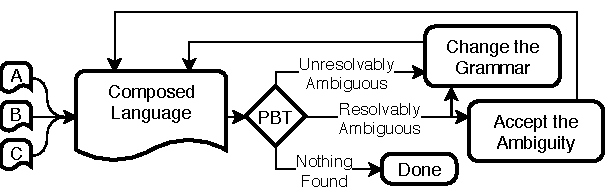
\includegraphics[scale=1.1]{figures/language-designer-workflow.pdf}
  \end{center} \pause

  \vfill
  \begin{center}
    %% Creator: Matplotlib, PGF backend
%%
%% To include the figure in your LaTeX document, write
%%   \input{<filename>.pgf}
%%
%% Make sure the required packages are loaded in your preamble
%%   \usepackage{pgf}
%%
%% Also ensure that all the required font packages are loaded; for instance,
%% the lmodern package is sometimes necessary when using math font.
%%   \usepackage{lmodern}
%%
%% Figures using additional raster images can only be included by \input if
%% they are in the same directory as the main LaTeX file. For loading figures
%% from other directories you can use the `import` package
%%   \usepackage{import}
%%
%% and then include the figures with
%%   \import{<path to file>}{<filename>.pgf}
%%
%% Matplotlib used the following preamble
%%   \def\mathdefault#1{#1}
%%   \everymath=\expandafter{\the\everymath\displaystyle}
%%   
%%   \usepackage{fontspec}
%%   \setmainfont{DejaVuSerif.ttf}[Path=\detokenize{/nix/store/289wryq1na3b9gccnyimh1238dqnmvvv-python3.11-matplotlib-3.8.3/lib/python3.11/site-packages/matplotlib/mpl-data/fonts/ttf/}]
%%   \setsansfont{DejaVuSans.ttf}[Path=\detokenize{/nix/store/289wryq1na3b9gccnyimh1238dqnmvvv-python3.11-matplotlib-3.8.3/lib/python3.11/site-packages/matplotlib/mpl-data/fonts/ttf/}]
%%   \setmonofont{DejaVuSansMono.ttf}[Path=\detokenize{/nix/store/289wryq1na3b9gccnyimh1238dqnmvvv-python3.11-matplotlib-3.8.3/lib/python3.11/site-packages/matplotlib/mpl-data/fonts/ttf/}]
%%   \makeatletter\@ifpackageloaded{underscore}{}{\usepackage[strings]{underscore}}\makeatother
%%
\begingroup%
\makeatletter%
\begin{pgfpicture}%
\pgfpathrectangle{\pgfpointorigin}{\pgfqpoint{2.310000in}{1.700000in}}%
\pgfusepath{use as bounding box, clip}%
\begin{pgfscope}%
\pgfsetbuttcap%
\pgfsetmiterjoin%
\definecolor{currentfill}{rgb}{1.000000,1.000000,1.000000}%
\pgfsetfillcolor{currentfill}%
\pgfsetlinewidth{0.000000pt}%
\definecolor{currentstroke}{rgb}{1.000000,1.000000,1.000000}%
\pgfsetstrokecolor{currentstroke}%
\pgfsetdash{}{0pt}%
\pgfpathmoveto{\pgfqpoint{0.000000in}{0.000000in}}%
\pgfpathlineto{\pgfqpoint{2.310000in}{0.000000in}}%
\pgfpathlineto{\pgfqpoint{2.310000in}{1.700000in}}%
\pgfpathlineto{\pgfqpoint{0.000000in}{1.700000in}}%
\pgfpathlineto{\pgfqpoint{0.000000in}{0.000000in}}%
\pgfpathclose%
\pgfusepath{fill}%
\end{pgfscope}%
\begin{pgfscope}%
\pgfsetbuttcap%
\pgfsetmiterjoin%
\definecolor{currentfill}{rgb}{1.000000,1.000000,1.000000}%
\pgfsetfillcolor{currentfill}%
\pgfsetlinewidth{0.000000pt}%
\definecolor{currentstroke}{rgb}{0.000000,0.000000,0.000000}%
\pgfsetstrokecolor{currentstroke}%
\pgfsetstrokeopacity{0.000000}%
\pgfsetdash{}{0pt}%
\pgfpathmoveto{\pgfqpoint{0.752778in}{0.582778in}}%
\pgfpathlineto{\pgfqpoint{2.146123in}{0.582778in}}%
\pgfpathlineto{\pgfqpoint{2.146123in}{1.495000in}}%
\pgfpathlineto{\pgfqpoint{0.752778in}{1.495000in}}%
\pgfpathlineto{\pgfqpoint{0.752778in}{0.582778in}}%
\pgfpathclose%
\pgfusepath{fill}%
\end{pgfscope}%
\begin{pgfscope}%
\pgfpathrectangle{\pgfqpoint{0.752778in}{0.582778in}}{\pgfqpoint{1.393345in}{0.912222in}}%
\pgfusepath{clip}%
\pgfsetrectcap%
\pgfsetroundjoin%
\pgfsetlinewidth{0.803000pt}%
\definecolor{currentstroke}{rgb}{0.690196,0.690196,0.690196}%
\pgfsetstrokecolor{currentstroke}%
\pgfsetdash{}{0pt}%
\pgfpathmoveto{\pgfqpoint{0.816072in}{0.582778in}}%
\pgfpathlineto{\pgfqpoint{0.816072in}{1.495000in}}%
\pgfusepath{stroke}%
\end{pgfscope}%
\begin{pgfscope}%
\pgfsetbuttcap%
\pgfsetroundjoin%
\definecolor{currentfill}{rgb}{0.000000,0.000000,0.000000}%
\pgfsetfillcolor{currentfill}%
\pgfsetlinewidth{0.803000pt}%
\definecolor{currentstroke}{rgb}{0.000000,0.000000,0.000000}%
\pgfsetstrokecolor{currentstroke}%
\pgfsetdash{}{0pt}%
\pgfsys@defobject{currentmarker}{\pgfqpoint{0.000000in}{-0.048611in}}{\pgfqpoint{0.000000in}{0.000000in}}{%
\pgfpathmoveto{\pgfqpoint{0.000000in}{0.000000in}}%
\pgfpathlineto{\pgfqpoint{0.000000in}{-0.048611in}}%
\pgfusepath{stroke,fill}%
}%
\begin{pgfscope}%
\pgfsys@transformshift{0.816072in}{0.582778in}%
\pgfsys@useobject{currentmarker}{}%
\end{pgfscope}%
\end{pgfscope}%
\begin{pgfscope}%
\definecolor{textcolor}{rgb}{0.000000,0.000000,0.000000}%
\pgfsetstrokecolor{textcolor}%
\pgfsetfillcolor{textcolor}%
\pgftext[x=0.816072in,y=0.485556in,,top]{\color{textcolor}{\sffamily\fontsize{10.000000}{12.000000}\selectfont\catcode`\^=\active\def^{\ifmmode\sp\else\^{}\fi}\catcode`\%=\active\def%{\%}0}}%
\end{pgfscope}%
\begin{pgfscope}%
\pgfpathrectangle{\pgfqpoint{0.752778in}{0.582778in}}{\pgfqpoint{1.393345in}{0.912222in}}%
\pgfusepath{clip}%
\pgfsetrectcap%
\pgfsetroundjoin%
\pgfsetlinewidth{0.803000pt}%
\definecolor{currentstroke}{rgb}{0.690196,0.690196,0.690196}%
\pgfsetstrokecolor{currentstroke}%
\pgfsetdash{}{0pt}%
\pgfpathmoveto{\pgfqpoint{1.451961in}{0.582778in}}%
\pgfpathlineto{\pgfqpoint{1.451961in}{1.495000in}}%
\pgfusepath{stroke}%
\end{pgfscope}%
\begin{pgfscope}%
\pgfsetbuttcap%
\pgfsetroundjoin%
\definecolor{currentfill}{rgb}{0.000000,0.000000,0.000000}%
\pgfsetfillcolor{currentfill}%
\pgfsetlinewidth{0.803000pt}%
\definecolor{currentstroke}{rgb}{0.000000,0.000000,0.000000}%
\pgfsetstrokecolor{currentstroke}%
\pgfsetdash{}{0pt}%
\pgfsys@defobject{currentmarker}{\pgfqpoint{0.000000in}{-0.048611in}}{\pgfqpoint{0.000000in}{0.000000in}}{%
\pgfpathmoveto{\pgfqpoint{0.000000in}{0.000000in}}%
\pgfpathlineto{\pgfqpoint{0.000000in}{-0.048611in}}%
\pgfusepath{stroke,fill}%
}%
\begin{pgfscope}%
\pgfsys@transformshift{1.451961in}{0.582778in}%
\pgfsys@useobject{currentmarker}{}%
\end{pgfscope}%
\end{pgfscope}%
\begin{pgfscope}%
\definecolor{textcolor}{rgb}{0.000000,0.000000,0.000000}%
\pgfsetstrokecolor{textcolor}%
\pgfsetfillcolor{textcolor}%
\pgftext[x=1.451961in,y=0.485556in,,top]{\color{textcolor}{\sffamily\fontsize{10.000000}{12.000000}\selectfont\catcode`\^=\active\def^{\ifmmode\sp\else\^{}\fi}\catcode`\%=\active\def%{\%}5}}%
\end{pgfscope}%
\begin{pgfscope}%
\pgfpathrectangle{\pgfqpoint{0.752778in}{0.582778in}}{\pgfqpoint{1.393345in}{0.912222in}}%
\pgfusepath{clip}%
\pgfsetrectcap%
\pgfsetroundjoin%
\pgfsetlinewidth{0.803000pt}%
\definecolor{currentstroke}{rgb}{0.690196,0.690196,0.690196}%
\pgfsetstrokecolor{currentstroke}%
\pgfsetdash{}{0pt}%
\pgfpathmoveto{\pgfqpoint{2.087850in}{0.582778in}}%
\pgfpathlineto{\pgfqpoint{2.087850in}{1.495000in}}%
\pgfusepath{stroke}%
\end{pgfscope}%
\begin{pgfscope}%
\pgfsetbuttcap%
\pgfsetroundjoin%
\definecolor{currentfill}{rgb}{0.000000,0.000000,0.000000}%
\pgfsetfillcolor{currentfill}%
\pgfsetlinewidth{0.803000pt}%
\definecolor{currentstroke}{rgb}{0.000000,0.000000,0.000000}%
\pgfsetstrokecolor{currentstroke}%
\pgfsetdash{}{0pt}%
\pgfsys@defobject{currentmarker}{\pgfqpoint{0.000000in}{-0.048611in}}{\pgfqpoint{0.000000in}{0.000000in}}{%
\pgfpathmoveto{\pgfqpoint{0.000000in}{0.000000in}}%
\pgfpathlineto{\pgfqpoint{0.000000in}{-0.048611in}}%
\pgfusepath{stroke,fill}%
}%
\begin{pgfscope}%
\pgfsys@transformshift{2.087850in}{0.582778in}%
\pgfsys@useobject{currentmarker}{}%
\end{pgfscope}%
\end{pgfscope}%
\begin{pgfscope}%
\definecolor{textcolor}{rgb}{0.000000,0.000000,0.000000}%
\pgfsetstrokecolor{textcolor}%
\pgfsetfillcolor{textcolor}%
\pgftext[x=2.087850in,y=0.485556in,,top]{\color{textcolor}{\sffamily\fontsize{10.000000}{12.000000}\selectfont\catcode`\^=\active\def^{\ifmmode\sp\else\^{}\fi}\catcode`\%=\active\def%{\%}10}}%
\end{pgfscope}%
\begin{pgfscope}%
\pgfsetbuttcap%
\pgfsetroundjoin%
\definecolor{currentfill}{rgb}{0.000000,0.000000,0.000000}%
\pgfsetfillcolor{currentfill}%
\pgfsetlinewidth{0.602250pt}%
\definecolor{currentstroke}{rgb}{0.000000,0.000000,0.000000}%
\pgfsetstrokecolor{currentstroke}%
\pgfsetdash{}{0pt}%
\pgfsys@defobject{currentmarker}{\pgfqpoint{0.000000in}{-0.027778in}}{\pgfqpoint{0.000000in}{0.000000in}}{%
\pgfpathmoveto{\pgfqpoint{0.000000in}{0.000000in}}%
\pgfpathlineto{\pgfqpoint{0.000000in}{-0.027778in}}%
\pgfusepath{stroke,fill}%
}%
\begin{pgfscope}%
\pgfsys@transformshift{0.943250in}{0.582778in}%
\pgfsys@useobject{currentmarker}{}%
\end{pgfscope}%
\end{pgfscope}%
\begin{pgfscope}%
\pgfsetbuttcap%
\pgfsetroundjoin%
\definecolor{currentfill}{rgb}{0.000000,0.000000,0.000000}%
\pgfsetfillcolor{currentfill}%
\pgfsetlinewidth{0.602250pt}%
\definecolor{currentstroke}{rgb}{0.000000,0.000000,0.000000}%
\pgfsetstrokecolor{currentstroke}%
\pgfsetdash{}{0pt}%
\pgfsys@defobject{currentmarker}{\pgfqpoint{0.000000in}{-0.027778in}}{\pgfqpoint{0.000000in}{0.000000in}}{%
\pgfpathmoveto{\pgfqpoint{0.000000in}{0.000000in}}%
\pgfpathlineto{\pgfqpoint{0.000000in}{-0.027778in}}%
\pgfusepath{stroke,fill}%
}%
\begin{pgfscope}%
\pgfsys@transformshift{1.070428in}{0.582778in}%
\pgfsys@useobject{currentmarker}{}%
\end{pgfscope}%
\end{pgfscope}%
\begin{pgfscope}%
\pgfsetbuttcap%
\pgfsetroundjoin%
\definecolor{currentfill}{rgb}{0.000000,0.000000,0.000000}%
\pgfsetfillcolor{currentfill}%
\pgfsetlinewidth{0.602250pt}%
\definecolor{currentstroke}{rgb}{0.000000,0.000000,0.000000}%
\pgfsetstrokecolor{currentstroke}%
\pgfsetdash{}{0pt}%
\pgfsys@defobject{currentmarker}{\pgfqpoint{0.000000in}{-0.027778in}}{\pgfqpoint{0.000000in}{0.000000in}}{%
\pgfpathmoveto{\pgfqpoint{0.000000in}{0.000000in}}%
\pgfpathlineto{\pgfqpoint{0.000000in}{-0.027778in}}%
\pgfusepath{stroke,fill}%
}%
\begin{pgfscope}%
\pgfsys@transformshift{1.197605in}{0.582778in}%
\pgfsys@useobject{currentmarker}{}%
\end{pgfscope}%
\end{pgfscope}%
\begin{pgfscope}%
\pgfsetbuttcap%
\pgfsetroundjoin%
\definecolor{currentfill}{rgb}{0.000000,0.000000,0.000000}%
\pgfsetfillcolor{currentfill}%
\pgfsetlinewidth{0.602250pt}%
\definecolor{currentstroke}{rgb}{0.000000,0.000000,0.000000}%
\pgfsetstrokecolor{currentstroke}%
\pgfsetdash{}{0pt}%
\pgfsys@defobject{currentmarker}{\pgfqpoint{0.000000in}{-0.027778in}}{\pgfqpoint{0.000000in}{0.000000in}}{%
\pgfpathmoveto{\pgfqpoint{0.000000in}{0.000000in}}%
\pgfpathlineto{\pgfqpoint{0.000000in}{-0.027778in}}%
\pgfusepath{stroke,fill}%
}%
\begin{pgfscope}%
\pgfsys@transformshift{1.324783in}{0.582778in}%
\pgfsys@useobject{currentmarker}{}%
\end{pgfscope}%
\end{pgfscope}%
\begin{pgfscope}%
\pgfsetbuttcap%
\pgfsetroundjoin%
\definecolor{currentfill}{rgb}{0.000000,0.000000,0.000000}%
\pgfsetfillcolor{currentfill}%
\pgfsetlinewidth{0.602250pt}%
\definecolor{currentstroke}{rgb}{0.000000,0.000000,0.000000}%
\pgfsetstrokecolor{currentstroke}%
\pgfsetdash{}{0pt}%
\pgfsys@defobject{currentmarker}{\pgfqpoint{0.000000in}{-0.027778in}}{\pgfqpoint{0.000000in}{0.000000in}}{%
\pgfpathmoveto{\pgfqpoint{0.000000in}{0.000000in}}%
\pgfpathlineto{\pgfqpoint{0.000000in}{-0.027778in}}%
\pgfusepath{stroke,fill}%
}%
\begin{pgfscope}%
\pgfsys@transformshift{1.579139in}{0.582778in}%
\pgfsys@useobject{currentmarker}{}%
\end{pgfscope}%
\end{pgfscope}%
\begin{pgfscope}%
\pgfsetbuttcap%
\pgfsetroundjoin%
\definecolor{currentfill}{rgb}{0.000000,0.000000,0.000000}%
\pgfsetfillcolor{currentfill}%
\pgfsetlinewidth{0.602250pt}%
\definecolor{currentstroke}{rgb}{0.000000,0.000000,0.000000}%
\pgfsetstrokecolor{currentstroke}%
\pgfsetdash{}{0pt}%
\pgfsys@defobject{currentmarker}{\pgfqpoint{0.000000in}{-0.027778in}}{\pgfqpoint{0.000000in}{0.000000in}}{%
\pgfpathmoveto{\pgfqpoint{0.000000in}{0.000000in}}%
\pgfpathlineto{\pgfqpoint{0.000000in}{-0.027778in}}%
\pgfusepath{stroke,fill}%
}%
\begin{pgfscope}%
\pgfsys@transformshift{1.706316in}{0.582778in}%
\pgfsys@useobject{currentmarker}{}%
\end{pgfscope}%
\end{pgfscope}%
\begin{pgfscope}%
\pgfsetbuttcap%
\pgfsetroundjoin%
\definecolor{currentfill}{rgb}{0.000000,0.000000,0.000000}%
\pgfsetfillcolor{currentfill}%
\pgfsetlinewidth{0.602250pt}%
\definecolor{currentstroke}{rgb}{0.000000,0.000000,0.000000}%
\pgfsetstrokecolor{currentstroke}%
\pgfsetdash{}{0pt}%
\pgfsys@defobject{currentmarker}{\pgfqpoint{0.000000in}{-0.027778in}}{\pgfqpoint{0.000000in}{0.000000in}}{%
\pgfpathmoveto{\pgfqpoint{0.000000in}{0.000000in}}%
\pgfpathlineto{\pgfqpoint{0.000000in}{-0.027778in}}%
\pgfusepath{stroke,fill}%
}%
\begin{pgfscope}%
\pgfsys@transformshift{1.833494in}{0.582778in}%
\pgfsys@useobject{currentmarker}{}%
\end{pgfscope}%
\end{pgfscope}%
\begin{pgfscope}%
\pgfsetbuttcap%
\pgfsetroundjoin%
\definecolor{currentfill}{rgb}{0.000000,0.000000,0.000000}%
\pgfsetfillcolor{currentfill}%
\pgfsetlinewidth{0.602250pt}%
\definecolor{currentstroke}{rgb}{0.000000,0.000000,0.000000}%
\pgfsetstrokecolor{currentstroke}%
\pgfsetdash{}{0pt}%
\pgfsys@defobject{currentmarker}{\pgfqpoint{0.000000in}{-0.027778in}}{\pgfqpoint{0.000000in}{0.000000in}}{%
\pgfpathmoveto{\pgfqpoint{0.000000in}{0.000000in}}%
\pgfpathlineto{\pgfqpoint{0.000000in}{-0.027778in}}%
\pgfusepath{stroke,fill}%
}%
\begin{pgfscope}%
\pgfsys@transformshift{1.960672in}{0.582778in}%
\pgfsys@useobject{currentmarker}{}%
\end{pgfscope}%
\end{pgfscope}%
\begin{pgfscope}%
\definecolor{textcolor}{rgb}{0.000000,0.000000,0.000000}%
\pgfsetstrokecolor{textcolor}%
\pgfsetfillcolor{textcolor}%
\pgftext[x=1.449450in,y=0.295587in,,top]{\color{textcolor}{\sffamily\fontsize{10.000000}{12.000000}\selectfont\catcode`\^=\active\def^{\ifmmode\sp\else\^{}\fi}\catcode`\%=\active\def%{\%}Time (s)}}%
\end{pgfscope}%
\begin{pgfscope}%
\pgfpathrectangle{\pgfqpoint{0.752778in}{0.582778in}}{\pgfqpoint{1.393345in}{0.912222in}}%
\pgfusepath{clip}%
\pgfsetrectcap%
\pgfsetroundjoin%
\pgfsetlinewidth{0.803000pt}%
\definecolor{currentstroke}{rgb}{0.690196,0.690196,0.690196}%
\pgfsetstrokecolor{currentstroke}%
\pgfsetdash{}{0pt}%
\pgfpathmoveto{\pgfqpoint{0.752778in}{0.582778in}}%
\pgfpathlineto{\pgfqpoint{2.146123in}{0.582778in}}%
\pgfusepath{stroke}%
\end{pgfscope}%
\begin{pgfscope}%
\pgfsetbuttcap%
\pgfsetroundjoin%
\definecolor{currentfill}{rgb}{0.000000,0.000000,0.000000}%
\pgfsetfillcolor{currentfill}%
\pgfsetlinewidth{0.803000pt}%
\definecolor{currentstroke}{rgb}{0.000000,0.000000,0.000000}%
\pgfsetstrokecolor{currentstroke}%
\pgfsetdash{}{0pt}%
\pgfsys@defobject{currentmarker}{\pgfqpoint{-0.048611in}{0.000000in}}{\pgfqpoint{-0.000000in}{0.000000in}}{%
\pgfpathmoveto{\pgfqpoint{-0.000000in}{0.000000in}}%
\pgfpathlineto{\pgfqpoint{-0.048611in}{0.000000in}}%
\pgfusepath{stroke,fill}%
}%
\begin{pgfscope}%
\pgfsys@transformshift{0.752778in}{0.582778in}%
\pgfsys@useobject{currentmarker}{}%
\end{pgfscope}%
\end{pgfscope}%
\begin{pgfscope}%
\definecolor{textcolor}{rgb}{0.000000,0.000000,0.000000}%
\pgfsetstrokecolor{textcolor}%
\pgfsetfillcolor{textcolor}%
\pgftext[x=0.434676in, y=0.530016in, left, base]{\color{textcolor}{\sffamily\fontsize{10.000000}{12.000000}\selectfont\catcode`\^=\active\def^{\ifmmode\sp\else\^{}\fi}\catcode`\%=\active\def%{\%}0.0}}%
\end{pgfscope}%
\begin{pgfscope}%
\pgfpathrectangle{\pgfqpoint{0.752778in}{0.582778in}}{\pgfqpoint{1.393345in}{0.912222in}}%
\pgfusepath{clip}%
\pgfsetrectcap%
\pgfsetroundjoin%
\pgfsetlinewidth{0.803000pt}%
\definecolor{currentstroke}{rgb}{0.690196,0.690196,0.690196}%
\pgfsetstrokecolor{currentstroke}%
\pgfsetdash{}{0pt}%
\pgfpathmoveto{\pgfqpoint{0.752778in}{1.038889in}}%
\pgfpathlineto{\pgfqpoint{2.146123in}{1.038889in}}%
\pgfusepath{stroke}%
\end{pgfscope}%
\begin{pgfscope}%
\pgfsetbuttcap%
\pgfsetroundjoin%
\definecolor{currentfill}{rgb}{0.000000,0.000000,0.000000}%
\pgfsetfillcolor{currentfill}%
\pgfsetlinewidth{0.803000pt}%
\definecolor{currentstroke}{rgb}{0.000000,0.000000,0.000000}%
\pgfsetstrokecolor{currentstroke}%
\pgfsetdash{}{0pt}%
\pgfsys@defobject{currentmarker}{\pgfqpoint{-0.048611in}{0.000000in}}{\pgfqpoint{-0.000000in}{0.000000in}}{%
\pgfpathmoveto{\pgfqpoint{-0.000000in}{0.000000in}}%
\pgfpathlineto{\pgfqpoint{-0.048611in}{0.000000in}}%
\pgfusepath{stroke,fill}%
}%
\begin{pgfscope}%
\pgfsys@transformshift{0.752778in}{1.038889in}%
\pgfsys@useobject{currentmarker}{}%
\end{pgfscope}%
\end{pgfscope}%
\begin{pgfscope}%
\definecolor{textcolor}{rgb}{0.000000,0.000000,0.000000}%
\pgfsetstrokecolor{textcolor}%
\pgfsetfillcolor{textcolor}%
\pgftext[x=0.434676in, y=0.986127in, left, base]{\color{textcolor}{\sffamily\fontsize{10.000000}{12.000000}\selectfont\catcode`\^=\active\def^{\ifmmode\sp\else\^{}\fi}\catcode`\%=\active\def%{\%}0.5}}%
\end{pgfscope}%
\begin{pgfscope}%
\pgfpathrectangle{\pgfqpoint{0.752778in}{0.582778in}}{\pgfqpoint{1.393345in}{0.912222in}}%
\pgfusepath{clip}%
\pgfsetrectcap%
\pgfsetroundjoin%
\pgfsetlinewidth{0.803000pt}%
\definecolor{currentstroke}{rgb}{0.690196,0.690196,0.690196}%
\pgfsetstrokecolor{currentstroke}%
\pgfsetdash{}{0pt}%
\pgfpathmoveto{\pgfqpoint{0.752778in}{1.495000in}}%
\pgfpathlineto{\pgfqpoint{2.146123in}{1.495000in}}%
\pgfusepath{stroke}%
\end{pgfscope}%
\begin{pgfscope}%
\pgfsetbuttcap%
\pgfsetroundjoin%
\definecolor{currentfill}{rgb}{0.000000,0.000000,0.000000}%
\pgfsetfillcolor{currentfill}%
\pgfsetlinewidth{0.803000pt}%
\definecolor{currentstroke}{rgb}{0.000000,0.000000,0.000000}%
\pgfsetstrokecolor{currentstroke}%
\pgfsetdash{}{0pt}%
\pgfsys@defobject{currentmarker}{\pgfqpoint{-0.048611in}{0.000000in}}{\pgfqpoint{-0.000000in}{0.000000in}}{%
\pgfpathmoveto{\pgfqpoint{-0.000000in}{0.000000in}}%
\pgfpathlineto{\pgfqpoint{-0.048611in}{0.000000in}}%
\pgfusepath{stroke,fill}%
}%
\begin{pgfscope}%
\pgfsys@transformshift{0.752778in}{1.495000in}%
\pgfsys@useobject{currentmarker}{}%
\end{pgfscope}%
\end{pgfscope}%
\begin{pgfscope}%
\definecolor{textcolor}{rgb}{0.000000,0.000000,0.000000}%
\pgfsetstrokecolor{textcolor}%
\pgfsetfillcolor{textcolor}%
\pgftext[x=0.434676in, y=1.442238in, left, base]{\color{textcolor}{\sffamily\fontsize{10.000000}{12.000000}\selectfont\catcode`\^=\active\def^{\ifmmode\sp\else\^{}\fi}\catcode`\%=\active\def%{\%}1.0}}%
\end{pgfscope}%
\begin{pgfscope}%
\definecolor{textcolor}{rgb}{0.000000,0.000000,0.000000}%
\pgfsetstrokecolor{textcolor}%
\pgfsetfillcolor{textcolor}%
\pgftext[x=0.379121in,y=1.038889in,,bottom,rotate=90.000000]{\color{textcolor}{\sffamily\fontsize{10.000000}{12.000000}\selectfont\catcode`\^=\active\def^{\ifmmode\sp\else\^{}\fi}\catcode`\%=\active\def%{\%}Cumulative Freq.}}%
\end{pgfscope}%
\begin{pgfscope}%
\pgfpathrectangle{\pgfqpoint{0.752778in}{0.582778in}}{\pgfqpoint{1.393345in}{0.912222in}}%
\pgfusepath{clip}%
\pgfsetrectcap%
\pgfsetroundjoin%
\pgfsetlinewidth{1.505625pt}%
\definecolor{currentstroke}{rgb}{0.121569,0.466667,0.705882}%
\pgfsetstrokecolor{currentstroke}%
\pgfsetdash{}{0pt}%
\pgfpathmoveto{\pgfqpoint{0.816112in}{0.582792in}}%
\pgfpathlineto{\pgfqpoint{0.816263in}{0.606793in}}%
\pgfpathlineto{\pgfqpoint{0.818421in}{1.084299in}}%
\pgfpathlineto{\pgfqpoint{0.824789in}{1.255597in}}%
\pgfpathlineto{\pgfqpoint{0.826873in}{1.266616in}}%
\pgfpathlineto{\pgfqpoint{0.828051in}{1.271980in}}%
\pgfpathlineto{\pgfqpoint{0.830208in}{1.280843in}}%
\pgfpathlineto{\pgfqpoint{0.834100in}{1.294253in}}%
\pgfpathlineto{\pgfqpoint{0.834790in}{1.296866in}}%
\pgfpathlineto{\pgfqpoint{0.836224in}{1.301996in}}%
\pgfpathlineto{\pgfqpoint{0.837367in}{1.306876in}}%
\pgfpathlineto{\pgfqpoint{0.839319in}{1.312227in}}%
\pgfpathlineto{\pgfqpoint{0.839869in}{1.313803in}}%
\pgfpathlineto{\pgfqpoint{0.842236in}{1.318448in}}%
\pgfpathlineto{\pgfqpoint{0.850583in}{1.330614in}}%
\pgfpathlineto{\pgfqpoint{0.853299in}{1.338149in}}%
\pgfpathlineto{\pgfqpoint{0.855549in}{1.342560in}}%
\pgfpathlineto{\pgfqpoint{0.857630in}{1.345892in}}%
\pgfpathlineto{\pgfqpoint{0.863188in}{1.350703in}}%
\pgfpathlineto{\pgfqpoint{0.865732in}{1.353026in}}%
\pgfpathlineto{\pgfqpoint{0.869593in}{1.355155in}}%
\pgfpathlineto{\pgfqpoint{0.870706in}{1.356109in}}%
\pgfpathlineto{\pgfqpoint{0.872792in}{1.357436in}}%
\pgfpathlineto{\pgfqpoint{0.877760in}{1.359192in}}%
\pgfpathlineto{\pgfqpoint{0.878804in}{1.359524in}}%
\pgfpathlineto{\pgfqpoint{0.883850in}{1.361072in}}%
\pgfpathlineto{\pgfqpoint{0.885858in}{1.362081in}}%
\pgfpathlineto{\pgfqpoint{0.909919in}{1.370681in}}%
\pgfpathlineto{\pgfqpoint{0.932982in}{1.374939in}}%
\pgfpathlineto{\pgfqpoint{0.934098in}{1.375326in}}%
\pgfpathlineto{\pgfqpoint{0.941644in}{1.377054in}}%
\pgfpathlineto{\pgfqpoint{0.970848in}{1.383138in}}%
\pgfpathlineto{\pgfqpoint{0.973594in}{1.383857in}}%
\pgfpathlineto{\pgfqpoint{0.983503in}{1.385516in}}%
\pgfpathlineto{\pgfqpoint{0.984755in}{1.385806in}}%
\pgfpathlineto{\pgfqpoint{1.061162in}{1.397046in}}%
\pgfpathlineto{\pgfqpoint{1.112815in}{1.399936in}}%
\pgfpathlineto{\pgfqpoint{1.296860in}{1.409766in}}%
\pgfpathlineto{\pgfqpoint{1.431240in}{1.412876in}}%
\pgfpathlineto{\pgfqpoint{1.436407in}{1.413098in}}%
\pgfpathlineto{\pgfqpoint{1.511668in}{1.417715in}}%
\pgfpathlineto{\pgfqpoint{1.551896in}{1.418973in}}%
\pgfpathlineto{\pgfqpoint{1.591427in}{1.419997in}}%
\pgfpathlineto{\pgfqpoint{1.667373in}{1.421849in}}%
\pgfpathlineto{\pgfqpoint{1.676913in}{1.422070in}}%
\pgfpathlineto{\pgfqpoint{1.715990in}{1.422775in}}%
\pgfpathlineto{\pgfqpoint{1.903791in}{1.425416in}}%
\pgfpathlineto{\pgfqpoint{1.908934in}{1.425527in}}%
\pgfpathlineto{\pgfqpoint{2.082789in}{1.426730in}}%
\pgfpathlineto{\pgfqpoint{2.082789in}{1.426730in}}%
\pgfusepath{stroke}%
\end{pgfscope}%
\begin{pgfscope}%
\pgfsetrectcap%
\pgfsetmiterjoin%
\pgfsetlinewidth{0.803000pt}%
\definecolor{currentstroke}{rgb}{0.000000,0.000000,0.000000}%
\pgfsetstrokecolor{currentstroke}%
\pgfsetdash{}{0pt}%
\pgfpathmoveto{\pgfqpoint{0.752778in}{0.582778in}}%
\pgfpathlineto{\pgfqpoint{0.752778in}{1.495000in}}%
\pgfusepath{stroke}%
\end{pgfscope}%
\begin{pgfscope}%
\pgfsetrectcap%
\pgfsetmiterjoin%
\pgfsetlinewidth{0.803000pt}%
\definecolor{currentstroke}{rgb}{0.000000,0.000000,0.000000}%
\pgfsetstrokecolor{currentstroke}%
\pgfsetdash{}{0pt}%
\pgfpathmoveto{\pgfqpoint{2.146123in}{0.582778in}}%
\pgfpathlineto{\pgfqpoint{2.146123in}{1.495000in}}%
\pgfusepath{stroke}%
\end{pgfscope}%
\begin{pgfscope}%
\pgfsetrectcap%
\pgfsetmiterjoin%
\pgfsetlinewidth{0.803000pt}%
\definecolor{currentstroke}{rgb}{0.000000,0.000000,0.000000}%
\pgfsetstrokecolor{currentstroke}%
\pgfsetdash{}{0pt}%
\pgfpathmoveto{\pgfqpoint{0.752778in}{0.582778in}}%
\pgfpathlineto{\pgfqpoint{2.146123in}{0.582778in}}%
\pgfusepath{stroke}%
\end{pgfscope}%
\begin{pgfscope}%
\pgfsetrectcap%
\pgfsetmiterjoin%
\pgfsetlinewidth{0.803000pt}%
\definecolor{currentstroke}{rgb}{0.000000,0.000000,0.000000}%
\pgfsetstrokecolor{currentstroke}%
\pgfsetdash{}{0pt}%
\pgfpathmoveto{\pgfqpoint{0.752778in}{1.495000in}}%
\pgfpathlineto{\pgfqpoint{2.146123in}{1.495000in}}%
\pgfusepath{stroke}%
\end{pgfscope}%
\end{pgfpicture}%
\makeatother%
\endgroup%
 \pause
    %% Creator: Matplotlib, PGF backend
%%
%% To include the figure in your LaTeX document, write
%%   \input{<filename>.pgf}
%%
%% Make sure the required packages are loaded in your preamble
%%   \usepackage{pgf}
%%
%% Also ensure that all the required font packages are loaded; for instance,
%% the lmodern package is sometimes necessary when using math font.
%%   \usepackage{lmodern}
%%
%% Figures using additional raster images can only be included by \input if
%% they are in the same directory as the main LaTeX file. For loading figures
%% from other directories you can use the `import` package
%%   \usepackage{import}
%%
%% and then include the figures with
%%   \import{<path to file>}{<filename>.pgf}
%%
%% Matplotlib used the following preamble
%%   \def\mathdefault#1{#1}
%%   \everymath=\expandafter{\the\everymath\displaystyle}
%%   
%%   \usepackage{fontspec}
%%   \setmainfont{DejaVuSerif.ttf}[Path=\detokenize{/nix/store/289wryq1na3b9gccnyimh1238dqnmvvv-python3.11-matplotlib-3.8.3/lib/python3.11/site-packages/matplotlib/mpl-data/fonts/ttf/}]
%%   \setsansfont{DejaVuSans.ttf}[Path=\detokenize{/nix/store/289wryq1na3b9gccnyimh1238dqnmvvv-python3.11-matplotlib-3.8.3/lib/python3.11/site-packages/matplotlib/mpl-data/fonts/ttf/}]
%%   \setmonofont{DejaVuSansMono.ttf}[Path=\detokenize{/nix/store/289wryq1na3b9gccnyimh1238dqnmvvv-python3.11-matplotlib-3.8.3/lib/python3.11/site-packages/matplotlib/mpl-data/fonts/ttf/}]
%%   \makeatletter\@ifpackageloaded{underscore}{}{\usepackage[strings]{underscore}}\makeatother
%%
\begingroup%
\makeatletter%
\begin{pgfpicture}%
\pgfpathrectangle{\pgfpointorigin}{\pgfqpoint{2.310000in}{1.700000in}}%
\pgfusepath{use as bounding box, clip}%
\begin{pgfscope}%
\pgfsetbuttcap%
\pgfsetmiterjoin%
\definecolor{currentfill}{rgb}{1.000000,1.000000,1.000000}%
\pgfsetfillcolor{currentfill}%
\pgfsetlinewidth{0.000000pt}%
\definecolor{currentstroke}{rgb}{1.000000,1.000000,1.000000}%
\pgfsetstrokecolor{currentstroke}%
\pgfsetdash{}{0pt}%
\pgfpathmoveto{\pgfqpoint{0.000000in}{0.000000in}}%
\pgfpathlineto{\pgfqpoint{2.310000in}{0.000000in}}%
\pgfpathlineto{\pgfqpoint{2.310000in}{1.700000in}}%
\pgfpathlineto{\pgfqpoint{0.000000in}{1.700000in}}%
\pgfpathlineto{\pgfqpoint{0.000000in}{0.000000in}}%
\pgfpathclose%
\pgfusepath{fill}%
\end{pgfscope}%
\begin{pgfscope}%
\pgfsetbuttcap%
\pgfsetmiterjoin%
\definecolor{currentfill}{rgb}{1.000000,1.000000,1.000000}%
\pgfsetfillcolor{currentfill}%
\pgfsetlinewidth{0.000000pt}%
\definecolor{currentstroke}{rgb}{0.000000,0.000000,0.000000}%
\pgfsetstrokecolor{currentstroke}%
\pgfsetstrokeopacity{0.000000}%
\pgfsetdash{}{0pt}%
\pgfpathmoveto{\pgfqpoint{0.620278in}{0.582778in}}%
\pgfpathlineto{\pgfqpoint{2.160000in}{0.582778in}}%
\pgfpathlineto{\pgfqpoint{2.160000in}{1.550000in}}%
\pgfpathlineto{\pgfqpoint{0.620278in}{1.550000in}}%
\pgfpathlineto{\pgfqpoint{0.620278in}{0.582778in}}%
\pgfpathclose%
\pgfusepath{fill}%
\end{pgfscope}%
\begin{pgfscope}%
\pgfpathrectangle{\pgfqpoint{0.620278in}{0.582778in}}{\pgfqpoint{1.539722in}{0.967222in}}%
\pgfusepath{clip}%
\pgfsetbuttcap%
\pgfsetroundjoin%
\definecolor{currentfill}{rgb}{0.000000,0.600000,0.533333}%
\pgfsetfillcolor{currentfill}%
\pgfsetlinewidth{0.000000pt}%
\definecolor{currentstroke}{rgb}{0.000000,0.000000,0.000000}%
\pgfsetstrokecolor{currentstroke}%
\pgfsetdash{}{0pt}%
\pgfpathmoveto{\pgfqpoint{0.690265in}{1.388796in}}%
\pgfpathlineto{\pgfqpoint{0.690265in}{0.582778in}}%
\pgfpathlineto{\pgfqpoint{0.698748in}{0.582778in}}%
\pgfpathlineto{\pgfqpoint{0.707232in}{0.582778in}}%
\pgfpathlineto{\pgfqpoint{0.715715in}{0.582778in}}%
\pgfpathlineto{\pgfqpoint{0.724198in}{0.582778in}}%
\pgfpathlineto{\pgfqpoint{0.732682in}{0.582778in}}%
\pgfpathlineto{\pgfqpoint{0.741165in}{0.582778in}}%
\pgfpathlineto{\pgfqpoint{0.749648in}{0.582778in}}%
\pgfpathlineto{\pgfqpoint{0.758132in}{0.582778in}}%
\pgfpathlineto{\pgfqpoint{0.766615in}{0.582778in}}%
\pgfpathlineto{\pgfqpoint{0.775098in}{0.582778in}}%
\pgfpathlineto{\pgfqpoint{0.783582in}{0.582778in}}%
\pgfpathlineto{\pgfqpoint{0.792065in}{0.582778in}}%
\pgfpathlineto{\pgfqpoint{0.800548in}{0.582778in}}%
\pgfpathlineto{\pgfqpoint{0.809032in}{0.582778in}}%
\pgfpathlineto{\pgfqpoint{0.817515in}{0.582778in}}%
\pgfpathlineto{\pgfqpoint{0.825998in}{0.582778in}}%
\pgfpathlineto{\pgfqpoint{0.834482in}{0.582778in}}%
\pgfpathlineto{\pgfqpoint{0.842965in}{0.582778in}}%
\pgfpathlineto{\pgfqpoint{0.851448in}{0.582778in}}%
\pgfpathlineto{\pgfqpoint{0.859932in}{0.582778in}}%
\pgfpathlineto{\pgfqpoint{0.868415in}{0.582778in}}%
\pgfpathlineto{\pgfqpoint{0.876898in}{0.582778in}}%
\pgfpathlineto{\pgfqpoint{0.885381in}{0.582778in}}%
\pgfpathlineto{\pgfqpoint{0.893865in}{0.582778in}}%
\pgfpathlineto{\pgfqpoint{0.902348in}{0.582778in}}%
\pgfpathlineto{\pgfqpoint{0.910831in}{0.582778in}}%
\pgfpathlineto{\pgfqpoint{0.919315in}{0.582778in}}%
\pgfpathlineto{\pgfqpoint{0.927798in}{0.582778in}}%
\pgfpathlineto{\pgfqpoint{0.936281in}{0.582778in}}%
\pgfpathlineto{\pgfqpoint{0.944765in}{0.582778in}}%
\pgfpathlineto{\pgfqpoint{0.953248in}{0.582778in}}%
\pgfpathlineto{\pgfqpoint{0.961731in}{0.582778in}}%
\pgfpathlineto{\pgfqpoint{0.970215in}{0.582778in}}%
\pgfpathlineto{\pgfqpoint{0.978698in}{0.582778in}}%
\pgfpathlineto{\pgfqpoint{0.987181in}{0.582778in}}%
\pgfpathlineto{\pgfqpoint{0.995665in}{0.582778in}}%
\pgfpathlineto{\pgfqpoint{1.004148in}{0.582778in}}%
\pgfpathlineto{\pgfqpoint{1.012631in}{0.582778in}}%
\pgfpathlineto{\pgfqpoint{1.021115in}{0.582778in}}%
\pgfpathlineto{\pgfqpoint{1.029598in}{0.582778in}}%
\pgfpathlineto{\pgfqpoint{1.038081in}{0.582778in}}%
\pgfpathlineto{\pgfqpoint{1.046565in}{0.582778in}}%
\pgfpathlineto{\pgfqpoint{1.055048in}{0.582778in}}%
\pgfpathlineto{\pgfqpoint{1.063531in}{0.582778in}}%
\pgfpathlineto{\pgfqpoint{1.072014in}{0.582778in}}%
\pgfpathlineto{\pgfqpoint{1.080498in}{0.582778in}}%
\pgfpathlineto{\pgfqpoint{1.088981in}{0.582778in}}%
\pgfpathlineto{\pgfqpoint{1.097464in}{0.582778in}}%
\pgfpathlineto{\pgfqpoint{1.105948in}{0.582778in}}%
\pgfpathlineto{\pgfqpoint{1.114431in}{0.582778in}}%
\pgfpathlineto{\pgfqpoint{1.122914in}{0.582778in}}%
\pgfpathlineto{\pgfqpoint{1.131398in}{0.582778in}}%
\pgfpathlineto{\pgfqpoint{1.139881in}{0.582778in}}%
\pgfpathlineto{\pgfqpoint{1.148364in}{0.582778in}}%
\pgfpathlineto{\pgfqpoint{1.156848in}{0.582778in}}%
\pgfpathlineto{\pgfqpoint{1.165331in}{0.582778in}}%
\pgfpathlineto{\pgfqpoint{1.173814in}{0.582778in}}%
\pgfpathlineto{\pgfqpoint{1.182298in}{0.582778in}}%
\pgfpathlineto{\pgfqpoint{1.190781in}{0.582778in}}%
\pgfpathlineto{\pgfqpoint{1.199264in}{0.582778in}}%
\pgfpathlineto{\pgfqpoint{1.207748in}{0.582778in}}%
\pgfpathlineto{\pgfqpoint{1.216231in}{0.582778in}}%
\pgfpathlineto{\pgfqpoint{1.224714in}{0.582778in}}%
\pgfpathlineto{\pgfqpoint{1.233198in}{0.582778in}}%
\pgfpathlineto{\pgfqpoint{1.241681in}{0.582778in}}%
\pgfpathlineto{\pgfqpoint{1.250164in}{0.582778in}}%
\pgfpathlineto{\pgfqpoint{1.258647in}{0.582778in}}%
\pgfpathlineto{\pgfqpoint{1.267131in}{0.582778in}}%
\pgfpathlineto{\pgfqpoint{1.275614in}{0.582778in}}%
\pgfpathlineto{\pgfqpoint{1.284097in}{0.582778in}}%
\pgfpathlineto{\pgfqpoint{1.292581in}{0.582778in}}%
\pgfpathlineto{\pgfqpoint{1.301064in}{0.582778in}}%
\pgfpathlineto{\pgfqpoint{1.309547in}{0.582778in}}%
\pgfpathlineto{\pgfqpoint{1.318031in}{0.582778in}}%
\pgfpathlineto{\pgfqpoint{1.326514in}{0.582778in}}%
\pgfpathlineto{\pgfqpoint{1.334997in}{0.582778in}}%
\pgfpathlineto{\pgfqpoint{1.343481in}{0.582778in}}%
\pgfpathlineto{\pgfqpoint{1.351964in}{0.582778in}}%
\pgfpathlineto{\pgfqpoint{1.360447in}{0.582778in}}%
\pgfpathlineto{\pgfqpoint{1.368931in}{0.582778in}}%
\pgfpathlineto{\pgfqpoint{1.377414in}{0.582778in}}%
\pgfpathlineto{\pgfqpoint{1.385897in}{0.582778in}}%
\pgfpathlineto{\pgfqpoint{1.394381in}{0.582778in}}%
\pgfpathlineto{\pgfqpoint{1.402864in}{0.582778in}}%
\pgfpathlineto{\pgfqpoint{1.411347in}{0.582778in}}%
\pgfpathlineto{\pgfqpoint{1.419831in}{0.582778in}}%
\pgfpathlineto{\pgfqpoint{1.428314in}{0.582778in}}%
\pgfpathlineto{\pgfqpoint{1.436797in}{0.582778in}}%
\pgfpathlineto{\pgfqpoint{1.445280in}{0.582778in}}%
\pgfpathlineto{\pgfqpoint{1.453764in}{0.582778in}}%
\pgfpathlineto{\pgfqpoint{1.462247in}{0.582778in}}%
\pgfpathlineto{\pgfqpoint{1.470730in}{0.582778in}}%
\pgfpathlineto{\pgfqpoint{1.479214in}{0.582778in}}%
\pgfpathlineto{\pgfqpoint{1.487697in}{0.582778in}}%
\pgfpathlineto{\pgfqpoint{1.496180in}{0.582778in}}%
\pgfpathlineto{\pgfqpoint{1.504664in}{0.582778in}}%
\pgfpathlineto{\pgfqpoint{1.513147in}{0.582778in}}%
\pgfpathlineto{\pgfqpoint{1.521630in}{0.582778in}}%
\pgfpathlineto{\pgfqpoint{1.530114in}{0.582778in}}%
\pgfpathlineto{\pgfqpoint{1.538597in}{0.582778in}}%
\pgfpathlineto{\pgfqpoint{1.547080in}{0.582778in}}%
\pgfpathlineto{\pgfqpoint{1.555564in}{0.582778in}}%
\pgfpathlineto{\pgfqpoint{1.564047in}{0.582778in}}%
\pgfpathlineto{\pgfqpoint{1.572530in}{0.582778in}}%
\pgfpathlineto{\pgfqpoint{1.581014in}{0.582778in}}%
\pgfpathlineto{\pgfqpoint{1.589497in}{0.582778in}}%
\pgfpathlineto{\pgfqpoint{1.597980in}{0.582778in}}%
\pgfpathlineto{\pgfqpoint{1.606463in}{0.582778in}}%
\pgfpathlineto{\pgfqpoint{1.614947in}{0.582778in}}%
\pgfpathlineto{\pgfqpoint{1.623430in}{0.582778in}}%
\pgfpathlineto{\pgfqpoint{1.631913in}{0.582778in}}%
\pgfpathlineto{\pgfqpoint{1.640397in}{0.582778in}}%
\pgfpathlineto{\pgfqpoint{1.648880in}{0.582778in}}%
\pgfpathlineto{\pgfqpoint{1.657363in}{0.582778in}}%
\pgfpathlineto{\pgfqpoint{1.665847in}{0.582778in}}%
\pgfpathlineto{\pgfqpoint{1.674330in}{0.582778in}}%
\pgfpathlineto{\pgfqpoint{1.682813in}{0.582778in}}%
\pgfpathlineto{\pgfqpoint{1.691297in}{0.582778in}}%
\pgfpathlineto{\pgfqpoint{1.699780in}{0.582778in}}%
\pgfpathlineto{\pgfqpoint{1.708263in}{0.582778in}}%
\pgfpathlineto{\pgfqpoint{1.716747in}{0.582778in}}%
\pgfpathlineto{\pgfqpoint{1.725230in}{0.582778in}}%
\pgfpathlineto{\pgfqpoint{1.733713in}{0.582778in}}%
\pgfpathlineto{\pgfqpoint{1.742197in}{0.582778in}}%
\pgfpathlineto{\pgfqpoint{1.750680in}{0.582778in}}%
\pgfpathlineto{\pgfqpoint{1.759163in}{0.582778in}}%
\pgfpathlineto{\pgfqpoint{1.767647in}{0.582778in}}%
\pgfpathlineto{\pgfqpoint{1.776130in}{0.582778in}}%
\pgfpathlineto{\pgfqpoint{1.784613in}{0.582778in}}%
\pgfpathlineto{\pgfqpoint{1.793096in}{0.582778in}}%
\pgfpathlineto{\pgfqpoint{1.801580in}{0.582778in}}%
\pgfpathlineto{\pgfqpoint{1.810063in}{0.582778in}}%
\pgfpathlineto{\pgfqpoint{1.818546in}{0.582778in}}%
\pgfpathlineto{\pgfqpoint{1.827030in}{0.582778in}}%
\pgfpathlineto{\pgfqpoint{1.835513in}{0.582778in}}%
\pgfpathlineto{\pgfqpoint{1.843996in}{0.582778in}}%
\pgfpathlineto{\pgfqpoint{1.852480in}{0.582778in}}%
\pgfpathlineto{\pgfqpoint{1.860963in}{0.582778in}}%
\pgfpathlineto{\pgfqpoint{1.869446in}{0.582778in}}%
\pgfpathlineto{\pgfqpoint{1.877930in}{0.582778in}}%
\pgfpathlineto{\pgfqpoint{1.886413in}{0.582778in}}%
\pgfpathlineto{\pgfqpoint{1.894896in}{0.582778in}}%
\pgfpathlineto{\pgfqpoint{1.903380in}{0.582778in}}%
\pgfpathlineto{\pgfqpoint{1.911863in}{0.582778in}}%
\pgfpathlineto{\pgfqpoint{1.920346in}{0.582778in}}%
\pgfpathlineto{\pgfqpoint{1.928830in}{0.582778in}}%
\pgfpathlineto{\pgfqpoint{1.937313in}{0.582778in}}%
\pgfpathlineto{\pgfqpoint{1.945796in}{0.582778in}}%
\pgfpathlineto{\pgfqpoint{1.954280in}{0.582778in}}%
\pgfpathlineto{\pgfqpoint{1.962763in}{0.582778in}}%
\pgfpathlineto{\pgfqpoint{1.971246in}{0.582778in}}%
\pgfpathlineto{\pgfqpoint{1.979729in}{0.582778in}}%
\pgfpathlineto{\pgfqpoint{1.988213in}{0.582778in}}%
\pgfpathlineto{\pgfqpoint{1.996696in}{0.582778in}}%
\pgfpathlineto{\pgfqpoint{2.005179in}{0.582778in}}%
\pgfpathlineto{\pgfqpoint{2.013663in}{0.582778in}}%
\pgfpathlineto{\pgfqpoint{2.022146in}{0.582778in}}%
\pgfpathlineto{\pgfqpoint{2.030629in}{0.582778in}}%
\pgfpathlineto{\pgfqpoint{2.039113in}{0.582778in}}%
\pgfpathlineto{\pgfqpoint{2.047596in}{0.582778in}}%
\pgfpathlineto{\pgfqpoint{2.056079in}{0.582778in}}%
\pgfpathlineto{\pgfqpoint{2.064563in}{0.582778in}}%
\pgfpathlineto{\pgfqpoint{2.073046in}{0.582778in}}%
\pgfpathlineto{\pgfqpoint{2.081529in}{0.582778in}}%
\pgfpathlineto{\pgfqpoint{2.090013in}{0.582778in}}%
\pgfpathlineto{\pgfqpoint{2.090013in}{0.582778in}}%
\pgfpathlineto{\pgfqpoint{2.090013in}{0.582778in}}%
\pgfpathlineto{\pgfqpoint{2.081529in}{0.582778in}}%
\pgfpathlineto{\pgfqpoint{2.073046in}{0.582778in}}%
\pgfpathlineto{\pgfqpoint{2.064563in}{0.582778in}}%
\pgfpathlineto{\pgfqpoint{2.056079in}{0.582778in}}%
\pgfpathlineto{\pgfqpoint{2.047596in}{0.582778in}}%
\pgfpathlineto{\pgfqpoint{2.039113in}{0.582778in}}%
\pgfpathlineto{\pgfqpoint{2.030629in}{0.582778in}}%
\pgfpathlineto{\pgfqpoint{2.022146in}{0.582778in}}%
\pgfpathlineto{\pgfqpoint{2.013663in}{0.582778in}}%
\pgfpathlineto{\pgfqpoint{2.005179in}{0.582778in}}%
\pgfpathlineto{\pgfqpoint{1.996696in}{0.582778in}}%
\pgfpathlineto{\pgfqpoint{1.988213in}{0.582778in}}%
\pgfpathlineto{\pgfqpoint{1.979729in}{0.582778in}}%
\pgfpathlineto{\pgfqpoint{1.971246in}{0.582778in}}%
\pgfpathlineto{\pgfqpoint{1.962763in}{0.582778in}}%
\pgfpathlineto{\pgfqpoint{1.954280in}{0.582778in}}%
\pgfpathlineto{\pgfqpoint{1.945796in}{0.582778in}}%
\pgfpathlineto{\pgfqpoint{1.937313in}{0.582778in}}%
\pgfpathlineto{\pgfqpoint{1.928830in}{0.582778in}}%
\pgfpathlineto{\pgfqpoint{1.920346in}{0.582778in}}%
\pgfpathlineto{\pgfqpoint{1.911863in}{0.582778in}}%
\pgfpathlineto{\pgfqpoint{1.903380in}{0.582778in}}%
\pgfpathlineto{\pgfqpoint{1.894896in}{0.582778in}}%
\pgfpathlineto{\pgfqpoint{1.886413in}{0.582778in}}%
\pgfpathlineto{\pgfqpoint{1.877930in}{0.582778in}}%
\pgfpathlineto{\pgfqpoint{1.869446in}{0.582778in}}%
\pgfpathlineto{\pgfqpoint{1.860963in}{0.582778in}}%
\pgfpathlineto{\pgfqpoint{1.852480in}{0.582778in}}%
\pgfpathlineto{\pgfqpoint{1.843996in}{0.582778in}}%
\pgfpathlineto{\pgfqpoint{1.835513in}{0.582778in}}%
\pgfpathlineto{\pgfqpoint{1.827030in}{0.582778in}}%
\pgfpathlineto{\pgfqpoint{1.818546in}{0.582778in}}%
\pgfpathlineto{\pgfqpoint{1.810063in}{0.582778in}}%
\pgfpathlineto{\pgfqpoint{1.801580in}{0.582778in}}%
\pgfpathlineto{\pgfqpoint{1.793096in}{0.582778in}}%
\pgfpathlineto{\pgfqpoint{1.784613in}{0.582778in}}%
\pgfpathlineto{\pgfqpoint{1.776130in}{0.582778in}}%
\pgfpathlineto{\pgfqpoint{1.767647in}{0.582778in}}%
\pgfpathlineto{\pgfqpoint{1.759163in}{0.582778in}}%
\pgfpathlineto{\pgfqpoint{1.750680in}{0.582778in}}%
\pgfpathlineto{\pgfqpoint{1.742197in}{0.582778in}}%
\pgfpathlineto{\pgfqpoint{1.733713in}{0.582778in}}%
\pgfpathlineto{\pgfqpoint{1.725230in}{0.582778in}}%
\pgfpathlineto{\pgfqpoint{1.716747in}{0.582778in}}%
\pgfpathlineto{\pgfqpoint{1.708263in}{0.582778in}}%
\pgfpathlineto{\pgfqpoint{1.699780in}{0.582778in}}%
\pgfpathlineto{\pgfqpoint{1.691297in}{0.582778in}}%
\pgfpathlineto{\pgfqpoint{1.682813in}{0.582778in}}%
\pgfpathlineto{\pgfqpoint{1.674330in}{0.582778in}}%
\pgfpathlineto{\pgfqpoint{1.665847in}{0.582778in}}%
\pgfpathlineto{\pgfqpoint{1.657363in}{0.582778in}}%
\pgfpathlineto{\pgfqpoint{1.648880in}{0.582778in}}%
\pgfpathlineto{\pgfqpoint{1.640397in}{0.582778in}}%
\pgfpathlineto{\pgfqpoint{1.631913in}{0.582778in}}%
\pgfpathlineto{\pgfqpoint{1.623430in}{0.582778in}}%
\pgfpathlineto{\pgfqpoint{1.614947in}{0.582778in}}%
\pgfpathlineto{\pgfqpoint{1.606463in}{0.582778in}}%
\pgfpathlineto{\pgfqpoint{1.597980in}{0.582778in}}%
\pgfpathlineto{\pgfqpoint{1.589497in}{0.582778in}}%
\pgfpathlineto{\pgfqpoint{1.581014in}{0.582778in}}%
\pgfpathlineto{\pgfqpoint{1.572530in}{0.582778in}}%
\pgfpathlineto{\pgfqpoint{1.564047in}{0.582778in}}%
\pgfpathlineto{\pgfqpoint{1.555564in}{0.582778in}}%
\pgfpathlineto{\pgfqpoint{1.547080in}{0.582778in}}%
\pgfpathlineto{\pgfqpoint{1.538597in}{0.582778in}}%
\pgfpathlineto{\pgfqpoint{1.530114in}{0.582778in}}%
\pgfpathlineto{\pgfqpoint{1.521630in}{0.582778in}}%
\pgfpathlineto{\pgfqpoint{1.513147in}{0.582778in}}%
\pgfpathlineto{\pgfqpoint{1.504664in}{0.582778in}}%
\pgfpathlineto{\pgfqpoint{1.496180in}{0.582778in}}%
\pgfpathlineto{\pgfqpoint{1.487697in}{0.582778in}}%
\pgfpathlineto{\pgfqpoint{1.479214in}{0.582778in}}%
\pgfpathlineto{\pgfqpoint{1.470730in}{0.582778in}}%
\pgfpathlineto{\pgfqpoint{1.462247in}{0.582778in}}%
\pgfpathlineto{\pgfqpoint{1.453764in}{0.582778in}}%
\pgfpathlineto{\pgfqpoint{1.445280in}{0.582778in}}%
\pgfpathlineto{\pgfqpoint{1.436797in}{0.582778in}}%
\pgfpathlineto{\pgfqpoint{1.428314in}{0.582778in}}%
\pgfpathlineto{\pgfqpoint{1.419831in}{0.582778in}}%
\pgfpathlineto{\pgfqpoint{1.411347in}{0.582778in}}%
\pgfpathlineto{\pgfqpoint{1.402864in}{0.582778in}}%
\pgfpathlineto{\pgfqpoint{1.394381in}{0.582778in}}%
\pgfpathlineto{\pgfqpoint{1.385897in}{0.582778in}}%
\pgfpathlineto{\pgfqpoint{1.377414in}{0.582778in}}%
\pgfpathlineto{\pgfqpoint{1.368931in}{0.582778in}}%
\pgfpathlineto{\pgfqpoint{1.360447in}{0.582778in}}%
\pgfpathlineto{\pgfqpoint{1.351964in}{0.582778in}}%
\pgfpathlineto{\pgfqpoint{1.343481in}{0.582778in}}%
\pgfpathlineto{\pgfqpoint{1.334997in}{0.582778in}}%
\pgfpathlineto{\pgfqpoint{1.326514in}{0.582778in}}%
\pgfpathlineto{\pgfqpoint{1.318031in}{0.582778in}}%
\pgfpathlineto{\pgfqpoint{1.309547in}{0.582778in}}%
\pgfpathlineto{\pgfqpoint{1.301064in}{0.582778in}}%
\pgfpathlineto{\pgfqpoint{1.292581in}{0.582778in}}%
\pgfpathlineto{\pgfqpoint{1.284097in}{0.582778in}}%
\pgfpathlineto{\pgfqpoint{1.275614in}{0.582778in}}%
\pgfpathlineto{\pgfqpoint{1.267131in}{0.582778in}}%
\pgfpathlineto{\pgfqpoint{1.258647in}{0.582778in}}%
\pgfpathlineto{\pgfqpoint{1.250164in}{0.582778in}}%
\pgfpathlineto{\pgfqpoint{1.241681in}{0.582778in}}%
\pgfpathlineto{\pgfqpoint{1.233198in}{0.582778in}}%
\pgfpathlineto{\pgfqpoint{1.224714in}{0.582778in}}%
\pgfpathlineto{\pgfqpoint{1.216231in}{0.582778in}}%
\pgfpathlineto{\pgfqpoint{1.207748in}{0.582778in}}%
\pgfpathlineto{\pgfqpoint{1.199264in}{0.582778in}}%
\pgfpathlineto{\pgfqpoint{1.190781in}{0.582778in}}%
\pgfpathlineto{\pgfqpoint{1.182298in}{0.582778in}}%
\pgfpathlineto{\pgfqpoint{1.173814in}{0.582778in}}%
\pgfpathlineto{\pgfqpoint{1.165331in}{0.582778in}}%
\pgfpathlineto{\pgfqpoint{1.156848in}{0.582778in}}%
\pgfpathlineto{\pgfqpoint{1.148364in}{0.582778in}}%
\pgfpathlineto{\pgfqpoint{1.139881in}{0.582778in}}%
\pgfpathlineto{\pgfqpoint{1.131398in}{0.582778in}}%
\pgfpathlineto{\pgfqpoint{1.122914in}{0.582778in}}%
\pgfpathlineto{\pgfqpoint{1.114431in}{0.582778in}}%
\pgfpathlineto{\pgfqpoint{1.105948in}{0.582778in}}%
\pgfpathlineto{\pgfqpoint{1.097464in}{0.582778in}}%
\pgfpathlineto{\pgfqpoint{1.088981in}{0.582778in}}%
\pgfpathlineto{\pgfqpoint{1.080498in}{0.582778in}}%
\pgfpathlineto{\pgfqpoint{1.072014in}{0.582778in}}%
\pgfpathlineto{\pgfqpoint{1.063531in}{0.582778in}}%
\pgfpathlineto{\pgfqpoint{1.055048in}{0.582778in}}%
\pgfpathlineto{\pgfqpoint{1.046565in}{0.582778in}}%
\pgfpathlineto{\pgfqpoint{1.038081in}{0.582778in}}%
\pgfpathlineto{\pgfqpoint{1.029598in}{0.582778in}}%
\pgfpathlineto{\pgfqpoint{1.021115in}{0.582778in}}%
\pgfpathlineto{\pgfqpoint{1.012631in}{0.582778in}}%
\pgfpathlineto{\pgfqpoint{1.004148in}{0.582778in}}%
\pgfpathlineto{\pgfqpoint{0.995665in}{0.582778in}}%
\pgfpathlineto{\pgfqpoint{0.987181in}{0.582778in}}%
\pgfpathlineto{\pgfqpoint{0.978698in}{0.582778in}}%
\pgfpathlineto{\pgfqpoint{0.970215in}{0.582778in}}%
\pgfpathlineto{\pgfqpoint{0.961731in}{0.582778in}}%
\pgfpathlineto{\pgfqpoint{0.953248in}{0.582778in}}%
\pgfpathlineto{\pgfqpoint{0.944765in}{0.582778in}}%
\pgfpathlineto{\pgfqpoint{0.936281in}{0.582778in}}%
\pgfpathlineto{\pgfqpoint{0.927798in}{0.582778in}}%
\pgfpathlineto{\pgfqpoint{0.919315in}{0.582778in}}%
\pgfpathlineto{\pgfqpoint{0.910831in}{0.582778in}}%
\pgfpathlineto{\pgfqpoint{0.902348in}{0.621160in}}%
\pgfpathlineto{\pgfqpoint{0.893865in}{0.582778in}}%
\pgfpathlineto{\pgfqpoint{0.885381in}{0.621160in}}%
\pgfpathlineto{\pgfqpoint{0.876898in}{0.621160in}}%
\pgfpathlineto{\pgfqpoint{0.868415in}{0.621160in}}%
\pgfpathlineto{\pgfqpoint{0.859932in}{0.582778in}}%
\pgfpathlineto{\pgfqpoint{0.851448in}{0.621160in}}%
\pgfpathlineto{\pgfqpoint{0.842965in}{0.659541in}}%
\pgfpathlineto{\pgfqpoint{0.834482in}{0.621160in}}%
\pgfpathlineto{\pgfqpoint{0.825998in}{0.582778in}}%
\pgfpathlineto{\pgfqpoint{0.817515in}{0.659541in}}%
\pgfpathlineto{\pgfqpoint{0.809032in}{0.659541in}}%
\pgfpathlineto{\pgfqpoint{0.800548in}{0.851451in}}%
\pgfpathlineto{\pgfqpoint{0.792065in}{0.928214in}}%
\pgfpathlineto{\pgfqpoint{0.783582in}{0.659541in}}%
\pgfpathlineto{\pgfqpoint{0.775098in}{0.889832in}}%
\pgfpathlineto{\pgfqpoint{0.766615in}{0.851451in}}%
\pgfpathlineto{\pgfqpoint{0.758132in}{0.851451in}}%
\pgfpathlineto{\pgfqpoint{0.749648in}{0.889832in}}%
\pgfpathlineto{\pgfqpoint{0.741165in}{0.966596in}}%
\pgfpathlineto{\pgfqpoint{0.732682in}{0.966596in}}%
\pgfpathlineto{\pgfqpoint{0.724198in}{0.851451in}}%
\pgfpathlineto{\pgfqpoint{0.715715in}{1.120123in}}%
\pgfpathlineto{\pgfqpoint{0.707232in}{0.889832in}}%
\pgfpathlineto{\pgfqpoint{0.698748in}{1.081742in}}%
\pgfpathlineto{\pgfqpoint{0.690265in}{1.388796in}}%
\pgfpathlineto{\pgfqpoint{0.690265in}{1.388796in}}%
\pgfpathclose%
\pgfusepath{fill}%
\end{pgfscope}%
\begin{pgfscope}%
\pgfpathrectangle{\pgfqpoint{0.620278in}{0.582778in}}{\pgfqpoint{1.539722in}{0.967222in}}%
\pgfusepath{clip}%
\pgfsetbuttcap%
\pgfsetroundjoin%
\definecolor{currentfill}{rgb}{0.200000,0.733333,0.933333}%
\pgfsetfillcolor{currentfill}%
\pgfsetlinewidth{0.000000pt}%
\definecolor{currentstroke}{rgb}{0.000000,0.000000,0.000000}%
\pgfsetstrokecolor{currentstroke}%
\pgfsetdash{}{0pt}%
\pgfpathmoveto{\pgfqpoint{0.690265in}{1.388796in}}%
\pgfpathlineto{\pgfqpoint{0.690265in}{1.388796in}}%
\pgfpathlineto{\pgfqpoint{0.698748in}{1.081742in}}%
\pgfpathlineto{\pgfqpoint{0.707232in}{0.889832in}}%
\pgfpathlineto{\pgfqpoint{0.715715in}{1.120123in}}%
\pgfpathlineto{\pgfqpoint{0.724198in}{0.851451in}}%
\pgfpathlineto{\pgfqpoint{0.732682in}{0.966596in}}%
\pgfpathlineto{\pgfqpoint{0.741165in}{0.966596in}}%
\pgfpathlineto{\pgfqpoint{0.749648in}{0.889832in}}%
\pgfpathlineto{\pgfqpoint{0.758132in}{0.851451in}}%
\pgfpathlineto{\pgfqpoint{0.766615in}{0.851451in}}%
\pgfpathlineto{\pgfqpoint{0.775098in}{0.889832in}}%
\pgfpathlineto{\pgfqpoint{0.783582in}{0.659541in}}%
\pgfpathlineto{\pgfqpoint{0.792065in}{0.928214in}}%
\pgfpathlineto{\pgfqpoint{0.800548in}{0.851451in}}%
\pgfpathlineto{\pgfqpoint{0.809032in}{0.659541in}}%
\pgfpathlineto{\pgfqpoint{0.817515in}{0.659541in}}%
\pgfpathlineto{\pgfqpoint{0.825998in}{0.582778in}}%
\pgfpathlineto{\pgfqpoint{0.834482in}{0.621160in}}%
\pgfpathlineto{\pgfqpoint{0.842965in}{0.659541in}}%
\pgfpathlineto{\pgfqpoint{0.851448in}{0.621160in}}%
\pgfpathlineto{\pgfqpoint{0.859932in}{0.582778in}}%
\pgfpathlineto{\pgfqpoint{0.868415in}{0.621160in}}%
\pgfpathlineto{\pgfqpoint{0.876898in}{0.621160in}}%
\pgfpathlineto{\pgfqpoint{0.885381in}{0.621160in}}%
\pgfpathlineto{\pgfqpoint{0.893865in}{0.582778in}}%
\pgfpathlineto{\pgfqpoint{0.902348in}{0.621160in}}%
\pgfpathlineto{\pgfqpoint{0.910831in}{0.582778in}}%
\pgfpathlineto{\pgfqpoint{0.919315in}{0.582778in}}%
\pgfpathlineto{\pgfqpoint{0.927798in}{0.582778in}}%
\pgfpathlineto{\pgfqpoint{0.936281in}{0.582778in}}%
\pgfpathlineto{\pgfqpoint{0.944765in}{0.582778in}}%
\pgfpathlineto{\pgfqpoint{0.953248in}{0.582778in}}%
\pgfpathlineto{\pgfqpoint{0.961731in}{0.582778in}}%
\pgfpathlineto{\pgfqpoint{0.970215in}{0.582778in}}%
\pgfpathlineto{\pgfqpoint{0.978698in}{0.582778in}}%
\pgfpathlineto{\pgfqpoint{0.987181in}{0.582778in}}%
\pgfpathlineto{\pgfqpoint{0.995665in}{0.582778in}}%
\pgfpathlineto{\pgfqpoint{1.004148in}{0.582778in}}%
\pgfpathlineto{\pgfqpoint{1.012631in}{0.582778in}}%
\pgfpathlineto{\pgfqpoint{1.021115in}{0.582778in}}%
\pgfpathlineto{\pgfqpoint{1.029598in}{0.582778in}}%
\pgfpathlineto{\pgfqpoint{1.038081in}{0.582778in}}%
\pgfpathlineto{\pgfqpoint{1.046565in}{0.582778in}}%
\pgfpathlineto{\pgfqpoint{1.055048in}{0.582778in}}%
\pgfpathlineto{\pgfqpoint{1.063531in}{0.582778in}}%
\pgfpathlineto{\pgfqpoint{1.072014in}{0.582778in}}%
\pgfpathlineto{\pgfqpoint{1.080498in}{0.582778in}}%
\pgfpathlineto{\pgfqpoint{1.088981in}{0.582778in}}%
\pgfpathlineto{\pgfqpoint{1.097464in}{0.582778in}}%
\pgfpathlineto{\pgfqpoint{1.105948in}{0.582778in}}%
\pgfpathlineto{\pgfqpoint{1.114431in}{0.582778in}}%
\pgfpathlineto{\pgfqpoint{1.122914in}{0.582778in}}%
\pgfpathlineto{\pgfqpoint{1.131398in}{0.582778in}}%
\pgfpathlineto{\pgfqpoint{1.139881in}{0.582778in}}%
\pgfpathlineto{\pgfqpoint{1.148364in}{0.582778in}}%
\pgfpathlineto{\pgfqpoint{1.156848in}{0.582778in}}%
\pgfpathlineto{\pgfqpoint{1.165331in}{0.582778in}}%
\pgfpathlineto{\pgfqpoint{1.173814in}{0.582778in}}%
\pgfpathlineto{\pgfqpoint{1.182298in}{0.582778in}}%
\pgfpathlineto{\pgfqpoint{1.190781in}{0.582778in}}%
\pgfpathlineto{\pgfqpoint{1.199264in}{0.582778in}}%
\pgfpathlineto{\pgfqpoint{1.207748in}{0.582778in}}%
\pgfpathlineto{\pgfqpoint{1.216231in}{0.582778in}}%
\pgfpathlineto{\pgfqpoint{1.224714in}{0.582778in}}%
\pgfpathlineto{\pgfqpoint{1.233198in}{0.582778in}}%
\pgfpathlineto{\pgfqpoint{1.241681in}{0.582778in}}%
\pgfpathlineto{\pgfqpoint{1.250164in}{0.582778in}}%
\pgfpathlineto{\pgfqpoint{1.258647in}{0.582778in}}%
\pgfpathlineto{\pgfqpoint{1.267131in}{0.582778in}}%
\pgfpathlineto{\pgfqpoint{1.275614in}{0.582778in}}%
\pgfpathlineto{\pgfqpoint{1.284097in}{0.582778in}}%
\pgfpathlineto{\pgfqpoint{1.292581in}{0.582778in}}%
\pgfpathlineto{\pgfqpoint{1.301064in}{0.582778in}}%
\pgfpathlineto{\pgfqpoint{1.309547in}{0.582778in}}%
\pgfpathlineto{\pgfqpoint{1.318031in}{0.582778in}}%
\pgfpathlineto{\pgfqpoint{1.326514in}{0.582778in}}%
\pgfpathlineto{\pgfqpoint{1.334997in}{0.582778in}}%
\pgfpathlineto{\pgfqpoint{1.343481in}{0.582778in}}%
\pgfpathlineto{\pgfqpoint{1.351964in}{0.582778in}}%
\pgfpathlineto{\pgfqpoint{1.360447in}{0.582778in}}%
\pgfpathlineto{\pgfqpoint{1.368931in}{0.582778in}}%
\pgfpathlineto{\pgfqpoint{1.377414in}{0.582778in}}%
\pgfpathlineto{\pgfqpoint{1.385897in}{0.582778in}}%
\pgfpathlineto{\pgfqpoint{1.394381in}{0.582778in}}%
\pgfpathlineto{\pgfqpoint{1.402864in}{0.582778in}}%
\pgfpathlineto{\pgfqpoint{1.411347in}{0.582778in}}%
\pgfpathlineto{\pgfqpoint{1.419831in}{0.582778in}}%
\pgfpathlineto{\pgfqpoint{1.428314in}{0.582778in}}%
\pgfpathlineto{\pgfqpoint{1.436797in}{0.582778in}}%
\pgfpathlineto{\pgfqpoint{1.445280in}{0.582778in}}%
\pgfpathlineto{\pgfqpoint{1.453764in}{0.582778in}}%
\pgfpathlineto{\pgfqpoint{1.462247in}{0.582778in}}%
\pgfpathlineto{\pgfqpoint{1.470730in}{0.582778in}}%
\pgfpathlineto{\pgfqpoint{1.479214in}{0.582778in}}%
\pgfpathlineto{\pgfqpoint{1.487697in}{0.582778in}}%
\pgfpathlineto{\pgfqpoint{1.496180in}{0.582778in}}%
\pgfpathlineto{\pgfqpoint{1.504664in}{0.582778in}}%
\pgfpathlineto{\pgfqpoint{1.513147in}{0.582778in}}%
\pgfpathlineto{\pgfqpoint{1.521630in}{0.582778in}}%
\pgfpathlineto{\pgfqpoint{1.530114in}{0.582778in}}%
\pgfpathlineto{\pgfqpoint{1.538597in}{0.582778in}}%
\pgfpathlineto{\pgfqpoint{1.547080in}{0.582778in}}%
\pgfpathlineto{\pgfqpoint{1.555564in}{0.582778in}}%
\pgfpathlineto{\pgfqpoint{1.564047in}{0.582778in}}%
\pgfpathlineto{\pgfqpoint{1.572530in}{0.582778in}}%
\pgfpathlineto{\pgfqpoint{1.581014in}{0.582778in}}%
\pgfpathlineto{\pgfqpoint{1.589497in}{0.582778in}}%
\pgfpathlineto{\pgfqpoint{1.597980in}{0.582778in}}%
\pgfpathlineto{\pgfqpoint{1.606463in}{0.582778in}}%
\pgfpathlineto{\pgfqpoint{1.614947in}{0.582778in}}%
\pgfpathlineto{\pgfqpoint{1.623430in}{0.582778in}}%
\pgfpathlineto{\pgfqpoint{1.631913in}{0.582778in}}%
\pgfpathlineto{\pgfqpoint{1.640397in}{0.582778in}}%
\pgfpathlineto{\pgfqpoint{1.648880in}{0.582778in}}%
\pgfpathlineto{\pgfqpoint{1.657363in}{0.582778in}}%
\pgfpathlineto{\pgfqpoint{1.665847in}{0.582778in}}%
\pgfpathlineto{\pgfqpoint{1.674330in}{0.582778in}}%
\pgfpathlineto{\pgfqpoint{1.682813in}{0.582778in}}%
\pgfpathlineto{\pgfqpoint{1.691297in}{0.582778in}}%
\pgfpathlineto{\pgfqpoint{1.699780in}{0.582778in}}%
\pgfpathlineto{\pgfqpoint{1.708263in}{0.582778in}}%
\pgfpathlineto{\pgfqpoint{1.716747in}{0.582778in}}%
\pgfpathlineto{\pgfqpoint{1.725230in}{0.582778in}}%
\pgfpathlineto{\pgfqpoint{1.733713in}{0.582778in}}%
\pgfpathlineto{\pgfqpoint{1.742197in}{0.582778in}}%
\pgfpathlineto{\pgfqpoint{1.750680in}{0.582778in}}%
\pgfpathlineto{\pgfqpoint{1.759163in}{0.582778in}}%
\pgfpathlineto{\pgfqpoint{1.767647in}{0.582778in}}%
\pgfpathlineto{\pgfqpoint{1.776130in}{0.582778in}}%
\pgfpathlineto{\pgfqpoint{1.784613in}{0.582778in}}%
\pgfpathlineto{\pgfqpoint{1.793096in}{0.582778in}}%
\pgfpathlineto{\pgfqpoint{1.801580in}{0.582778in}}%
\pgfpathlineto{\pgfqpoint{1.810063in}{0.582778in}}%
\pgfpathlineto{\pgfqpoint{1.818546in}{0.582778in}}%
\pgfpathlineto{\pgfqpoint{1.827030in}{0.582778in}}%
\pgfpathlineto{\pgfqpoint{1.835513in}{0.582778in}}%
\pgfpathlineto{\pgfqpoint{1.843996in}{0.582778in}}%
\pgfpathlineto{\pgfqpoint{1.852480in}{0.582778in}}%
\pgfpathlineto{\pgfqpoint{1.860963in}{0.582778in}}%
\pgfpathlineto{\pgfqpoint{1.869446in}{0.582778in}}%
\pgfpathlineto{\pgfqpoint{1.877930in}{0.582778in}}%
\pgfpathlineto{\pgfqpoint{1.886413in}{0.582778in}}%
\pgfpathlineto{\pgfqpoint{1.894896in}{0.582778in}}%
\pgfpathlineto{\pgfqpoint{1.903380in}{0.582778in}}%
\pgfpathlineto{\pgfqpoint{1.911863in}{0.582778in}}%
\pgfpathlineto{\pgfqpoint{1.920346in}{0.582778in}}%
\pgfpathlineto{\pgfqpoint{1.928830in}{0.582778in}}%
\pgfpathlineto{\pgfqpoint{1.937313in}{0.582778in}}%
\pgfpathlineto{\pgfqpoint{1.945796in}{0.582778in}}%
\pgfpathlineto{\pgfqpoint{1.954280in}{0.582778in}}%
\pgfpathlineto{\pgfqpoint{1.962763in}{0.582778in}}%
\pgfpathlineto{\pgfqpoint{1.971246in}{0.582778in}}%
\pgfpathlineto{\pgfqpoint{1.979729in}{0.582778in}}%
\pgfpathlineto{\pgfqpoint{1.988213in}{0.582778in}}%
\pgfpathlineto{\pgfqpoint{1.996696in}{0.582778in}}%
\pgfpathlineto{\pgfqpoint{2.005179in}{0.582778in}}%
\pgfpathlineto{\pgfqpoint{2.013663in}{0.582778in}}%
\pgfpathlineto{\pgfqpoint{2.022146in}{0.582778in}}%
\pgfpathlineto{\pgfqpoint{2.030629in}{0.582778in}}%
\pgfpathlineto{\pgfqpoint{2.039113in}{0.582778in}}%
\pgfpathlineto{\pgfqpoint{2.047596in}{0.582778in}}%
\pgfpathlineto{\pgfqpoint{2.056079in}{0.582778in}}%
\pgfpathlineto{\pgfqpoint{2.064563in}{0.582778in}}%
\pgfpathlineto{\pgfqpoint{2.073046in}{0.582778in}}%
\pgfpathlineto{\pgfqpoint{2.081529in}{0.582778in}}%
\pgfpathlineto{\pgfqpoint{2.090013in}{0.582778in}}%
\pgfpathlineto{\pgfqpoint{2.090013in}{0.582778in}}%
\pgfpathlineto{\pgfqpoint{2.090013in}{0.582778in}}%
\pgfpathlineto{\pgfqpoint{2.081529in}{0.582778in}}%
\pgfpathlineto{\pgfqpoint{2.073046in}{0.582778in}}%
\pgfpathlineto{\pgfqpoint{2.064563in}{0.582778in}}%
\pgfpathlineto{\pgfqpoint{2.056079in}{0.582778in}}%
\pgfpathlineto{\pgfqpoint{2.047596in}{0.582778in}}%
\pgfpathlineto{\pgfqpoint{2.039113in}{0.582778in}}%
\pgfpathlineto{\pgfqpoint{2.030629in}{0.582778in}}%
\pgfpathlineto{\pgfqpoint{2.022146in}{0.582778in}}%
\pgfpathlineto{\pgfqpoint{2.013663in}{0.582778in}}%
\pgfpathlineto{\pgfqpoint{2.005179in}{0.582778in}}%
\pgfpathlineto{\pgfqpoint{1.996696in}{0.582778in}}%
\pgfpathlineto{\pgfqpoint{1.988213in}{0.582778in}}%
\pgfpathlineto{\pgfqpoint{1.979729in}{0.582778in}}%
\pgfpathlineto{\pgfqpoint{1.971246in}{0.582778in}}%
\pgfpathlineto{\pgfqpoint{1.962763in}{0.621160in}}%
\pgfpathlineto{\pgfqpoint{1.954280in}{0.582778in}}%
\pgfpathlineto{\pgfqpoint{1.945796in}{0.582778in}}%
\pgfpathlineto{\pgfqpoint{1.937313in}{0.582778in}}%
\pgfpathlineto{\pgfqpoint{1.928830in}{0.582778in}}%
\pgfpathlineto{\pgfqpoint{1.920346in}{0.582778in}}%
\pgfpathlineto{\pgfqpoint{1.911863in}{0.582778in}}%
\pgfpathlineto{\pgfqpoint{1.903380in}{0.582778in}}%
\pgfpathlineto{\pgfqpoint{1.894896in}{0.582778in}}%
\pgfpathlineto{\pgfqpoint{1.886413in}{0.582778in}}%
\pgfpathlineto{\pgfqpoint{1.877930in}{0.582778in}}%
\pgfpathlineto{\pgfqpoint{1.869446in}{0.582778in}}%
\pgfpathlineto{\pgfqpoint{1.860963in}{0.582778in}}%
\pgfpathlineto{\pgfqpoint{1.852480in}{0.582778in}}%
\pgfpathlineto{\pgfqpoint{1.843996in}{0.582778in}}%
\pgfpathlineto{\pgfqpoint{1.835513in}{0.582778in}}%
\pgfpathlineto{\pgfqpoint{1.827030in}{0.582778in}}%
\pgfpathlineto{\pgfqpoint{1.818546in}{0.582778in}}%
\pgfpathlineto{\pgfqpoint{1.810063in}{0.582778in}}%
\pgfpathlineto{\pgfqpoint{1.801580in}{0.582778in}}%
\pgfpathlineto{\pgfqpoint{1.793096in}{0.582778in}}%
\pgfpathlineto{\pgfqpoint{1.784613in}{0.582778in}}%
\pgfpathlineto{\pgfqpoint{1.776130in}{0.582778in}}%
\pgfpathlineto{\pgfqpoint{1.767647in}{0.582778in}}%
\pgfpathlineto{\pgfqpoint{1.759163in}{0.582778in}}%
\pgfpathlineto{\pgfqpoint{1.750680in}{0.582778in}}%
\pgfpathlineto{\pgfqpoint{1.742197in}{0.582778in}}%
\pgfpathlineto{\pgfqpoint{1.733713in}{0.582778in}}%
\pgfpathlineto{\pgfqpoint{1.725230in}{0.582778in}}%
\pgfpathlineto{\pgfqpoint{1.716747in}{0.582778in}}%
\pgfpathlineto{\pgfqpoint{1.708263in}{0.582778in}}%
\pgfpathlineto{\pgfqpoint{1.699780in}{0.582778in}}%
\pgfpathlineto{\pgfqpoint{1.691297in}{0.582778in}}%
\pgfpathlineto{\pgfqpoint{1.682813in}{0.582778in}}%
\pgfpathlineto{\pgfqpoint{1.674330in}{0.582778in}}%
\pgfpathlineto{\pgfqpoint{1.665847in}{0.582778in}}%
\pgfpathlineto{\pgfqpoint{1.657363in}{0.621160in}}%
\pgfpathlineto{\pgfqpoint{1.648880in}{0.621160in}}%
\pgfpathlineto{\pgfqpoint{1.640397in}{0.582778in}}%
\pgfpathlineto{\pgfqpoint{1.631913in}{0.582778in}}%
\pgfpathlineto{\pgfqpoint{1.623430in}{0.582778in}}%
\pgfpathlineto{\pgfqpoint{1.614947in}{0.582778in}}%
\pgfpathlineto{\pgfqpoint{1.606463in}{0.582778in}}%
\pgfpathlineto{\pgfqpoint{1.597980in}{0.582778in}}%
\pgfpathlineto{\pgfqpoint{1.589497in}{0.582778in}}%
\pgfpathlineto{\pgfqpoint{1.581014in}{0.582778in}}%
\pgfpathlineto{\pgfqpoint{1.572530in}{0.582778in}}%
\pgfpathlineto{\pgfqpoint{1.564047in}{0.582778in}}%
\pgfpathlineto{\pgfqpoint{1.555564in}{0.582778in}}%
\pgfpathlineto{\pgfqpoint{1.547080in}{0.582778in}}%
\pgfpathlineto{\pgfqpoint{1.538597in}{0.582778in}}%
\pgfpathlineto{\pgfqpoint{1.530114in}{0.582778in}}%
\pgfpathlineto{\pgfqpoint{1.521630in}{0.582778in}}%
\pgfpathlineto{\pgfqpoint{1.513147in}{0.582778in}}%
\pgfpathlineto{\pgfqpoint{1.504664in}{0.582778in}}%
\pgfpathlineto{\pgfqpoint{1.496180in}{0.582778in}}%
\pgfpathlineto{\pgfqpoint{1.487697in}{0.582778in}}%
\pgfpathlineto{\pgfqpoint{1.479214in}{0.582778in}}%
\pgfpathlineto{\pgfqpoint{1.470730in}{0.621160in}}%
\pgfpathlineto{\pgfqpoint{1.462247in}{0.582778in}}%
\pgfpathlineto{\pgfqpoint{1.453764in}{0.582778in}}%
\pgfpathlineto{\pgfqpoint{1.445280in}{0.582778in}}%
\pgfpathlineto{\pgfqpoint{1.436797in}{0.582778in}}%
\pgfpathlineto{\pgfqpoint{1.428314in}{0.582778in}}%
\pgfpathlineto{\pgfqpoint{1.419831in}{0.621160in}}%
\pgfpathlineto{\pgfqpoint{1.411347in}{0.582778in}}%
\pgfpathlineto{\pgfqpoint{1.402864in}{0.582778in}}%
\pgfpathlineto{\pgfqpoint{1.394381in}{0.582778in}}%
\pgfpathlineto{\pgfqpoint{1.385897in}{0.621160in}}%
\pgfpathlineto{\pgfqpoint{1.377414in}{0.621160in}}%
\pgfpathlineto{\pgfqpoint{1.368931in}{0.621160in}}%
\pgfpathlineto{\pgfqpoint{1.360447in}{0.621160in}}%
\pgfpathlineto{\pgfqpoint{1.351964in}{0.582778in}}%
\pgfpathlineto{\pgfqpoint{1.343481in}{0.582778in}}%
\pgfpathlineto{\pgfqpoint{1.334997in}{0.621160in}}%
\pgfpathlineto{\pgfqpoint{1.326514in}{0.582778in}}%
\pgfpathlineto{\pgfqpoint{1.318031in}{0.582778in}}%
\pgfpathlineto{\pgfqpoint{1.309547in}{0.582778in}}%
\pgfpathlineto{\pgfqpoint{1.301064in}{0.621160in}}%
\pgfpathlineto{\pgfqpoint{1.292581in}{0.582778in}}%
\pgfpathlineto{\pgfqpoint{1.284097in}{0.621160in}}%
\pgfpathlineto{\pgfqpoint{1.275614in}{0.582778in}}%
\pgfpathlineto{\pgfqpoint{1.267131in}{0.582778in}}%
\pgfpathlineto{\pgfqpoint{1.258647in}{0.697923in}}%
\pgfpathlineto{\pgfqpoint{1.250164in}{0.697923in}}%
\pgfpathlineto{\pgfqpoint{1.241681in}{0.582778in}}%
\pgfpathlineto{\pgfqpoint{1.233198in}{0.582778in}}%
\pgfpathlineto{\pgfqpoint{1.224714in}{0.582778in}}%
\pgfpathlineto{\pgfqpoint{1.216231in}{0.582778in}}%
\pgfpathlineto{\pgfqpoint{1.207748in}{0.621160in}}%
\pgfpathlineto{\pgfqpoint{1.199264in}{0.582778in}}%
\pgfpathlineto{\pgfqpoint{1.190781in}{0.621160in}}%
\pgfpathlineto{\pgfqpoint{1.182298in}{0.659541in}}%
\pgfpathlineto{\pgfqpoint{1.173814in}{0.697923in}}%
\pgfpathlineto{\pgfqpoint{1.165331in}{0.621160in}}%
\pgfpathlineto{\pgfqpoint{1.156848in}{0.582778in}}%
\pgfpathlineto{\pgfqpoint{1.148364in}{0.659541in}}%
\pgfpathlineto{\pgfqpoint{1.139881in}{0.697923in}}%
\pgfpathlineto{\pgfqpoint{1.131398in}{0.659541in}}%
\pgfpathlineto{\pgfqpoint{1.122914in}{0.736305in}}%
\pgfpathlineto{\pgfqpoint{1.114431in}{0.621160in}}%
\pgfpathlineto{\pgfqpoint{1.105948in}{0.582778in}}%
\pgfpathlineto{\pgfqpoint{1.097464in}{0.659541in}}%
\pgfpathlineto{\pgfqpoint{1.088981in}{0.697923in}}%
\pgfpathlineto{\pgfqpoint{1.080498in}{0.621160in}}%
\pgfpathlineto{\pgfqpoint{1.072014in}{0.697923in}}%
\pgfpathlineto{\pgfqpoint{1.063531in}{0.697923in}}%
\pgfpathlineto{\pgfqpoint{1.055048in}{0.736305in}}%
\pgfpathlineto{\pgfqpoint{1.046565in}{0.736305in}}%
\pgfpathlineto{\pgfqpoint{1.038081in}{0.621160in}}%
\pgfpathlineto{\pgfqpoint{1.029598in}{0.928214in}}%
\pgfpathlineto{\pgfqpoint{1.021115in}{0.697923in}}%
\pgfpathlineto{\pgfqpoint{1.012631in}{0.736305in}}%
\pgfpathlineto{\pgfqpoint{1.004148in}{0.659541in}}%
\pgfpathlineto{\pgfqpoint{0.995665in}{0.697923in}}%
\pgfpathlineto{\pgfqpoint{0.987181in}{0.813069in}}%
\pgfpathlineto{\pgfqpoint{0.978698in}{0.813069in}}%
\pgfpathlineto{\pgfqpoint{0.970215in}{0.813069in}}%
\pgfpathlineto{\pgfqpoint{0.961731in}{0.736305in}}%
\pgfpathlineto{\pgfqpoint{0.953248in}{0.813069in}}%
\pgfpathlineto{\pgfqpoint{0.944765in}{0.813069in}}%
\pgfpathlineto{\pgfqpoint{0.936281in}{0.851451in}}%
\pgfpathlineto{\pgfqpoint{0.927798in}{0.813069in}}%
\pgfpathlineto{\pgfqpoint{0.919315in}{0.813069in}}%
\pgfpathlineto{\pgfqpoint{0.910831in}{0.928214in}}%
\pgfpathlineto{\pgfqpoint{0.902348in}{0.659541in}}%
\pgfpathlineto{\pgfqpoint{0.893865in}{1.043360in}}%
\pgfpathlineto{\pgfqpoint{0.885381in}{1.004978in}}%
\pgfpathlineto{\pgfqpoint{0.876898in}{0.889832in}}%
\pgfpathlineto{\pgfqpoint{0.868415in}{0.851451in}}%
\pgfpathlineto{\pgfqpoint{0.859932in}{0.966596in}}%
\pgfpathlineto{\pgfqpoint{0.851448in}{0.966596in}}%
\pgfpathlineto{\pgfqpoint{0.842965in}{1.081742in}}%
\pgfpathlineto{\pgfqpoint{0.834482in}{0.928214in}}%
\pgfpathlineto{\pgfqpoint{0.825998in}{0.851451in}}%
\pgfpathlineto{\pgfqpoint{0.817515in}{0.851451in}}%
\pgfpathlineto{\pgfqpoint{0.809032in}{0.813069in}}%
\pgfpathlineto{\pgfqpoint{0.800548in}{1.043360in}}%
\pgfpathlineto{\pgfqpoint{0.792065in}{1.312033in}}%
\pgfpathlineto{\pgfqpoint{0.783582in}{0.774687in}}%
\pgfpathlineto{\pgfqpoint{0.775098in}{1.043360in}}%
\pgfpathlineto{\pgfqpoint{0.766615in}{1.081742in}}%
\pgfpathlineto{\pgfqpoint{0.758132in}{1.120123in}}%
\pgfpathlineto{\pgfqpoint{0.749648in}{1.081742in}}%
\pgfpathlineto{\pgfqpoint{0.741165in}{1.120123in}}%
\pgfpathlineto{\pgfqpoint{0.732682in}{1.043360in}}%
\pgfpathlineto{\pgfqpoint{0.724198in}{0.851451in}}%
\pgfpathlineto{\pgfqpoint{0.715715in}{1.196887in}}%
\pgfpathlineto{\pgfqpoint{0.707232in}{0.889832in}}%
\pgfpathlineto{\pgfqpoint{0.698748in}{1.081742in}}%
\pgfpathlineto{\pgfqpoint{0.690265in}{1.388796in}}%
\pgfpathlineto{\pgfqpoint{0.690265in}{1.388796in}}%
\pgfpathclose%
\pgfusepath{fill}%
\end{pgfscope}%
\begin{pgfscope}%
\pgfpathrectangle{\pgfqpoint{0.620278in}{0.582778in}}{\pgfqpoint{1.539722in}{0.967222in}}%
\pgfusepath{clip}%
\pgfsetbuttcap%
\pgfsetroundjoin%
\definecolor{currentfill}{rgb}{0.000000,0.466667,0.733333}%
\pgfsetfillcolor{currentfill}%
\pgfsetlinewidth{0.000000pt}%
\definecolor{currentstroke}{rgb}{0.000000,0.000000,0.000000}%
\pgfsetstrokecolor{currentstroke}%
\pgfsetdash{}{0pt}%
\pgfpathmoveto{\pgfqpoint{0.690265in}{1.388796in}}%
\pgfpathlineto{\pgfqpoint{0.690265in}{1.388796in}}%
\pgfpathlineto{\pgfqpoint{0.698748in}{1.081742in}}%
\pgfpathlineto{\pgfqpoint{0.707232in}{0.889832in}}%
\pgfpathlineto{\pgfqpoint{0.715715in}{1.196887in}}%
\pgfpathlineto{\pgfqpoint{0.724198in}{0.851451in}}%
\pgfpathlineto{\pgfqpoint{0.732682in}{1.043360in}}%
\pgfpathlineto{\pgfqpoint{0.741165in}{1.120123in}}%
\pgfpathlineto{\pgfqpoint{0.749648in}{1.081742in}}%
\pgfpathlineto{\pgfqpoint{0.758132in}{1.120123in}}%
\pgfpathlineto{\pgfqpoint{0.766615in}{1.081742in}}%
\pgfpathlineto{\pgfqpoint{0.775098in}{1.043360in}}%
\pgfpathlineto{\pgfqpoint{0.783582in}{0.774687in}}%
\pgfpathlineto{\pgfqpoint{0.792065in}{1.312033in}}%
\pgfpathlineto{\pgfqpoint{0.800548in}{1.043360in}}%
\pgfpathlineto{\pgfqpoint{0.809032in}{0.813069in}}%
\pgfpathlineto{\pgfqpoint{0.817515in}{0.851451in}}%
\pgfpathlineto{\pgfqpoint{0.825998in}{0.851451in}}%
\pgfpathlineto{\pgfqpoint{0.834482in}{0.928214in}}%
\pgfpathlineto{\pgfqpoint{0.842965in}{1.081742in}}%
\pgfpathlineto{\pgfqpoint{0.851448in}{0.966596in}}%
\pgfpathlineto{\pgfqpoint{0.859932in}{0.966596in}}%
\pgfpathlineto{\pgfqpoint{0.868415in}{0.851451in}}%
\pgfpathlineto{\pgfqpoint{0.876898in}{0.889832in}}%
\pgfpathlineto{\pgfqpoint{0.885381in}{1.004978in}}%
\pgfpathlineto{\pgfqpoint{0.893865in}{1.043360in}}%
\pgfpathlineto{\pgfqpoint{0.902348in}{0.659541in}}%
\pgfpathlineto{\pgfqpoint{0.910831in}{0.928214in}}%
\pgfpathlineto{\pgfqpoint{0.919315in}{0.813069in}}%
\pgfpathlineto{\pgfqpoint{0.927798in}{0.813069in}}%
\pgfpathlineto{\pgfqpoint{0.936281in}{0.851451in}}%
\pgfpathlineto{\pgfqpoint{0.944765in}{0.813069in}}%
\pgfpathlineto{\pgfqpoint{0.953248in}{0.813069in}}%
\pgfpathlineto{\pgfqpoint{0.961731in}{0.736305in}}%
\pgfpathlineto{\pgfqpoint{0.970215in}{0.813069in}}%
\pgfpathlineto{\pgfqpoint{0.978698in}{0.813069in}}%
\pgfpathlineto{\pgfqpoint{0.987181in}{0.813069in}}%
\pgfpathlineto{\pgfqpoint{0.995665in}{0.697923in}}%
\pgfpathlineto{\pgfqpoint{1.004148in}{0.659541in}}%
\pgfpathlineto{\pgfqpoint{1.012631in}{0.736305in}}%
\pgfpathlineto{\pgfqpoint{1.021115in}{0.697923in}}%
\pgfpathlineto{\pgfqpoint{1.029598in}{0.928214in}}%
\pgfpathlineto{\pgfqpoint{1.038081in}{0.621160in}}%
\pgfpathlineto{\pgfqpoint{1.046565in}{0.736305in}}%
\pgfpathlineto{\pgfqpoint{1.055048in}{0.736305in}}%
\pgfpathlineto{\pgfqpoint{1.063531in}{0.697923in}}%
\pgfpathlineto{\pgfqpoint{1.072014in}{0.697923in}}%
\pgfpathlineto{\pgfqpoint{1.080498in}{0.621160in}}%
\pgfpathlineto{\pgfqpoint{1.088981in}{0.697923in}}%
\pgfpathlineto{\pgfqpoint{1.097464in}{0.659541in}}%
\pgfpathlineto{\pgfqpoint{1.105948in}{0.582778in}}%
\pgfpathlineto{\pgfqpoint{1.114431in}{0.621160in}}%
\pgfpathlineto{\pgfqpoint{1.122914in}{0.736305in}}%
\pgfpathlineto{\pgfqpoint{1.131398in}{0.659541in}}%
\pgfpathlineto{\pgfqpoint{1.139881in}{0.697923in}}%
\pgfpathlineto{\pgfqpoint{1.148364in}{0.659541in}}%
\pgfpathlineto{\pgfqpoint{1.156848in}{0.582778in}}%
\pgfpathlineto{\pgfqpoint{1.165331in}{0.621160in}}%
\pgfpathlineto{\pgfqpoint{1.173814in}{0.697923in}}%
\pgfpathlineto{\pgfqpoint{1.182298in}{0.659541in}}%
\pgfpathlineto{\pgfqpoint{1.190781in}{0.621160in}}%
\pgfpathlineto{\pgfqpoint{1.199264in}{0.582778in}}%
\pgfpathlineto{\pgfqpoint{1.207748in}{0.621160in}}%
\pgfpathlineto{\pgfqpoint{1.216231in}{0.582778in}}%
\pgfpathlineto{\pgfqpoint{1.224714in}{0.582778in}}%
\pgfpathlineto{\pgfqpoint{1.233198in}{0.582778in}}%
\pgfpathlineto{\pgfqpoint{1.241681in}{0.582778in}}%
\pgfpathlineto{\pgfqpoint{1.250164in}{0.697923in}}%
\pgfpathlineto{\pgfqpoint{1.258647in}{0.697923in}}%
\pgfpathlineto{\pgfqpoint{1.267131in}{0.582778in}}%
\pgfpathlineto{\pgfqpoint{1.275614in}{0.582778in}}%
\pgfpathlineto{\pgfqpoint{1.284097in}{0.621160in}}%
\pgfpathlineto{\pgfqpoint{1.292581in}{0.582778in}}%
\pgfpathlineto{\pgfqpoint{1.301064in}{0.621160in}}%
\pgfpathlineto{\pgfqpoint{1.309547in}{0.582778in}}%
\pgfpathlineto{\pgfqpoint{1.318031in}{0.582778in}}%
\pgfpathlineto{\pgfqpoint{1.326514in}{0.582778in}}%
\pgfpathlineto{\pgfqpoint{1.334997in}{0.621160in}}%
\pgfpathlineto{\pgfqpoint{1.343481in}{0.582778in}}%
\pgfpathlineto{\pgfqpoint{1.351964in}{0.582778in}}%
\pgfpathlineto{\pgfqpoint{1.360447in}{0.621160in}}%
\pgfpathlineto{\pgfqpoint{1.368931in}{0.621160in}}%
\pgfpathlineto{\pgfqpoint{1.377414in}{0.621160in}}%
\pgfpathlineto{\pgfqpoint{1.385897in}{0.621160in}}%
\pgfpathlineto{\pgfqpoint{1.394381in}{0.582778in}}%
\pgfpathlineto{\pgfqpoint{1.402864in}{0.582778in}}%
\pgfpathlineto{\pgfqpoint{1.411347in}{0.582778in}}%
\pgfpathlineto{\pgfqpoint{1.419831in}{0.621160in}}%
\pgfpathlineto{\pgfqpoint{1.428314in}{0.582778in}}%
\pgfpathlineto{\pgfqpoint{1.436797in}{0.582778in}}%
\pgfpathlineto{\pgfqpoint{1.445280in}{0.582778in}}%
\pgfpathlineto{\pgfqpoint{1.453764in}{0.582778in}}%
\pgfpathlineto{\pgfqpoint{1.462247in}{0.582778in}}%
\pgfpathlineto{\pgfqpoint{1.470730in}{0.621160in}}%
\pgfpathlineto{\pgfqpoint{1.479214in}{0.582778in}}%
\pgfpathlineto{\pgfqpoint{1.487697in}{0.582778in}}%
\pgfpathlineto{\pgfqpoint{1.496180in}{0.582778in}}%
\pgfpathlineto{\pgfqpoint{1.504664in}{0.582778in}}%
\pgfpathlineto{\pgfqpoint{1.513147in}{0.582778in}}%
\pgfpathlineto{\pgfqpoint{1.521630in}{0.582778in}}%
\pgfpathlineto{\pgfqpoint{1.530114in}{0.582778in}}%
\pgfpathlineto{\pgfqpoint{1.538597in}{0.582778in}}%
\pgfpathlineto{\pgfqpoint{1.547080in}{0.582778in}}%
\pgfpathlineto{\pgfqpoint{1.555564in}{0.582778in}}%
\pgfpathlineto{\pgfqpoint{1.564047in}{0.582778in}}%
\pgfpathlineto{\pgfqpoint{1.572530in}{0.582778in}}%
\pgfpathlineto{\pgfqpoint{1.581014in}{0.582778in}}%
\pgfpathlineto{\pgfqpoint{1.589497in}{0.582778in}}%
\pgfpathlineto{\pgfqpoint{1.597980in}{0.582778in}}%
\pgfpathlineto{\pgfqpoint{1.606463in}{0.582778in}}%
\pgfpathlineto{\pgfqpoint{1.614947in}{0.582778in}}%
\pgfpathlineto{\pgfqpoint{1.623430in}{0.582778in}}%
\pgfpathlineto{\pgfqpoint{1.631913in}{0.582778in}}%
\pgfpathlineto{\pgfqpoint{1.640397in}{0.582778in}}%
\pgfpathlineto{\pgfqpoint{1.648880in}{0.621160in}}%
\pgfpathlineto{\pgfqpoint{1.657363in}{0.621160in}}%
\pgfpathlineto{\pgfqpoint{1.665847in}{0.582778in}}%
\pgfpathlineto{\pgfqpoint{1.674330in}{0.582778in}}%
\pgfpathlineto{\pgfqpoint{1.682813in}{0.582778in}}%
\pgfpathlineto{\pgfqpoint{1.691297in}{0.582778in}}%
\pgfpathlineto{\pgfqpoint{1.699780in}{0.582778in}}%
\pgfpathlineto{\pgfqpoint{1.708263in}{0.582778in}}%
\pgfpathlineto{\pgfqpoint{1.716747in}{0.582778in}}%
\pgfpathlineto{\pgfqpoint{1.725230in}{0.582778in}}%
\pgfpathlineto{\pgfqpoint{1.733713in}{0.582778in}}%
\pgfpathlineto{\pgfqpoint{1.742197in}{0.582778in}}%
\pgfpathlineto{\pgfqpoint{1.750680in}{0.582778in}}%
\pgfpathlineto{\pgfqpoint{1.759163in}{0.582778in}}%
\pgfpathlineto{\pgfqpoint{1.767647in}{0.582778in}}%
\pgfpathlineto{\pgfqpoint{1.776130in}{0.582778in}}%
\pgfpathlineto{\pgfqpoint{1.784613in}{0.582778in}}%
\pgfpathlineto{\pgfqpoint{1.793096in}{0.582778in}}%
\pgfpathlineto{\pgfqpoint{1.801580in}{0.582778in}}%
\pgfpathlineto{\pgfqpoint{1.810063in}{0.582778in}}%
\pgfpathlineto{\pgfqpoint{1.818546in}{0.582778in}}%
\pgfpathlineto{\pgfqpoint{1.827030in}{0.582778in}}%
\pgfpathlineto{\pgfqpoint{1.835513in}{0.582778in}}%
\pgfpathlineto{\pgfqpoint{1.843996in}{0.582778in}}%
\pgfpathlineto{\pgfqpoint{1.852480in}{0.582778in}}%
\pgfpathlineto{\pgfqpoint{1.860963in}{0.582778in}}%
\pgfpathlineto{\pgfqpoint{1.869446in}{0.582778in}}%
\pgfpathlineto{\pgfqpoint{1.877930in}{0.582778in}}%
\pgfpathlineto{\pgfqpoint{1.886413in}{0.582778in}}%
\pgfpathlineto{\pgfqpoint{1.894896in}{0.582778in}}%
\pgfpathlineto{\pgfqpoint{1.903380in}{0.582778in}}%
\pgfpathlineto{\pgfqpoint{1.911863in}{0.582778in}}%
\pgfpathlineto{\pgfqpoint{1.920346in}{0.582778in}}%
\pgfpathlineto{\pgfqpoint{1.928830in}{0.582778in}}%
\pgfpathlineto{\pgfqpoint{1.937313in}{0.582778in}}%
\pgfpathlineto{\pgfqpoint{1.945796in}{0.582778in}}%
\pgfpathlineto{\pgfqpoint{1.954280in}{0.582778in}}%
\pgfpathlineto{\pgfqpoint{1.962763in}{0.621160in}}%
\pgfpathlineto{\pgfqpoint{1.971246in}{0.582778in}}%
\pgfpathlineto{\pgfqpoint{1.979729in}{0.582778in}}%
\pgfpathlineto{\pgfqpoint{1.988213in}{0.582778in}}%
\pgfpathlineto{\pgfqpoint{1.996696in}{0.582778in}}%
\pgfpathlineto{\pgfqpoint{2.005179in}{0.582778in}}%
\pgfpathlineto{\pgfqpoint{2.013663in}{0.582778in}}%
\pgfpathlineto{\pgfqpoint{2.022146in}{0.582778in}}%
\pgfpathlineto{\pgfqpoint{2.030629in}{0.582778in}}%
\pgfpathlineto{\pgfqpoint{2.039113in}{0.582778in}}%
\pgfpathlineto{\pgfqpoint{2.047596in}{0.582778in}}%
\pgfpathlineto{\pgfqpoint{2.056079in}{0.582778in}}%
\pgfpathlineto{\pgfqpoint{2.064563in}{0.582778in}}%
\pgfpathlineto{\pgfqpoint{2.073046in}{0.582778in}}%
\pgfpathlineto{\pgfqpoint{2.081529in}{0.582778in}}%
\pgfpathlineto{\pgfqpoint{2.090013in}{0.582778in}}%
\pgfpathlineto{\pgfqpoint{2.090013in}{0.582778in}}%
\pgfpathlineto{\pgfqpoint{2.090013in}{0.582778in}}%
\pgfpathlineto{\pgfqpoint{2.081529in}{0.582778in}}%
\pgfpathlineto{\pgfqpoint{2.073046in}{0.582778in}}%
\pgfpathlineto{\pgfqpoint{2.064563in}{0.582778in}}%
\pgfpathlineto{\pgfqpoint{2.056079in}{0.582778in}}%
\pgfpathlineto{\pgfqpoint{2.047596in}{0.582778in}}%
\pgfpathlineto{\pgfqpoint{2.039113in}{0.582778in}}%
\pgfpathlineto{\pgfqpoint{2.030629in}{0.582778in}}%
\pgfpathlineto{\pgfqpoint{2.022146in}{0.582778in}}%
\pgfpathlineto{\pgfqpoint{2.013663in}{0.582778in}}%
\pgfpathlineto{\pgfqpoint{2.005179in}{0.582778in}}%
\pgfpathlineto{\pgfqpoint{1.996696in}{0.582778in}}%
\pgfpathlineto{\pgfqpoint{1.988213in}{0.582778in}}%
\pgfpathlineto{\pgfqpoint{1.979729in}{0.582778in}}%
\pgfpathlineto{\pgfqpoint{1.971246in}{0.582778in}}%
\pgfpathlineto{\pgfqpoint{1.962763in}{0.621160in}}%
\pgfpathlineto{\pgfqpoint{1.954280in}{0.582778in}}%
\pgfpathlineto{\pgfqpoint{1.945796in}{0.582778in}}%
\pgfpathlineto{\pgfqpoint{1.937313in}{0.582778in}}%
\pgfpathlineto{\pgfqpoint{1.928830in}{0.582778in}}%
\pgfpathlineto{\pgfqpoint{1.920346in}{0.582778in}}%
\pgfpathlineto{\pgfqpoint{1.911863in}{0.582778in}}%
\pgfpathlineto{\pgfqpoint{1.903380in}{0.582778in}}%
\pgfpathlineto{\pgfqpoint{1.894896in}{0.582778in}}%
\pgfpathlineto{\pgfqpoint{1.886413in}{0.582778in}}%
\pgfpathlineto{\pgfqpoint{1.877930in}{0.582778in}}%
\pgfpathlineto{\pgfqpoint{1.869446in}{0.582778in}}%
\pgfpathlineto{\pgfqpoint{1.860963in}{0.582778in}}%
\pgfpathlineto{\pgfqpoint{1.852480in}{0.582778in}}%
\pgfpathlineto{\pgfqpoint{1.843996in}{0.582778in}}%
\pgfpathlineto{\pgfqpoint{1.835513in}{0.582778in}}%
\pgfpathlineto{\pgfqpoint{1.827030in}{0.582778in}}%
\pgfpathlineto{\pgfqpoint{1.818546in}{0.582778in}}%
\pgfpathlineto{\pgfqpoint{1.810063in}{0.582778in}}%
\pgfpathlineto{\pgfqpoint{1.801580in}{0.582778in}}%
\pgfpathlineto{\pgfqpoint{1.793096in}{0.582778in}}%
\pgfpathlineto{\pgfqpoint{1.784613in}{0.582778in}}%
\pgfpathlineto{\pgfqpoint{1.776130in}{0.582778in}}%
\pgfpathlineto{\pgfqpoint{1.767647in}{0.582778in}}%
\pgfpathlineto{\pgfqpoint{1.759163in}{0.582778in}}%
\pgfpathlineto{\pgfqpoint{1.750680in}{0.582778in}}%
\pgfpathlineto{\pgfqpoint{1.742197in}{0.582778in}}%
\pgfpathlineto{\pgfqpoint{1.733713in}{0.582778in}}%
\pgfpathlineto{\pgfqpoint{1.725230in}{0.582778in}}%
\pgfpathlineto{\pgfqpoint{1.716747in}{0.582778in}}%
\pgfpathlineto{\pgfqpoint{1.708263in}{0.582778in}}%
\pgfpathlineto{\pgfqpoint{1.699780in}{0.582778in}}%
\pgfpathlineto{\pgfqpoint{1.691297in}{0.582778in}}%
\pgfpathlineto{\pgfqpoint{1.682813in}{0.582778in}}%
\pgfpathlineto{\pgfqpoint{1.674330in}{0.582778in}}%
\pgfpathlineto{\pgfqpoint{1.665847in}{0.582778in}}%
\pgfpathlineto{\pgfqpoint{1.657363in}{0.621160in}}%
\pgfpathlineto{\pgfqpoint{1.648880in}{0.621160in}}%
\pgfpathlineto{\pgfqpoint{1.640397in}{0.582778in}}%
\pgfpathlineto{\pgfqpoint{1.631913in}{0.582778in}}%
\pgfpathlineto{\pgfqpoint{1.623430in}{0.582778in}}%
\pgfpathlineto{\pgfqpoint{1.614947in}{0.582778in}}%
\pgfpathlineto{\pgfqpoint{1.606463in}{0.582778in}}%
\pgfpathlineto{\pgfqpoint{1.597980in}{0.582778in}}%
\pgfpathlineto{\pgfqpoint{1.589497in}{0.582778in}}%
\pgfpathlineto{\pgfqpoint{1.581014in}{0.582778in}}%
\pgfpathlineto{\pgfqpoint{1.572530in}{0.582778in}}%
\pgfpathlineto{\pgfqpoint{1.564047in}{0.582778in}}%
\pgfpathlineto{\pgfqpoint{1.555564in}{0.582778in}}%
\pgfpathlineto{\pgfqpoint{1.547080in}{0.582778in}}%
\pgfpathlineto{\pgfqpoint{1.538597in}{0.582778in}}%
\pgfpathlineto{\pgfqpoint{1.530114in}{0.582778in}}%
\pgfpathlineto{\pgfqpoint{1.521630in}{0.582778in}}%
\pgfpathlineto{\pgfqpoint{1.513147in}{0.582778in}}%
\pgfpathlineto{\pgfqpoint{1.504664in}{0.582778in}}%
\pgfpathlineto{\pgfqpoint{1.496180in}{0.582778in}}%
\pgfpathlineto{\pgfqpoint{1.487697in}{0.582778in}}%
\pgfpathlineto{\pgfqpoint{1.479214in}{0.582778in}}%
\pgfpathlineto{\pgfqpoint{1.470730in}{0.621160in}}%
\pgfpathlineto{\pgfqpoint{1.462247in}{0.582778in}}%
\pgfpathlineto{\pgfqpoint{1.453764in}{0.582778in}}%
\pgfpathlineto{\pgfqpoint{1.445280in}{0.582778in}}%
\pgfpathlineto{\pgfqpoint{1.436797in}{0.582778in}}%
\pgfpathlineto{\pgfqpoint{1.428314in}{0.582778in}}%
\pgfpathlineto{\pgfqpoint{1.419831in}{0.621160in}}%
\pgfpathlineto{\pgfqpoint{1.411347in}{0.582778in}}%
\pgfpathlineto{\pgfqpoint{1.402864in}{0.582778in}}%
\pgfpathlineto{\pgfqpoint{1.394381in}{0.582778in}}%
\pgfpathlineto{\pgfqpoint{1.385897in}{0.621160in}}%
\pgfpathlineto{\pgfqpoint{1.377414in}{0.621160in}}%
\pgfpathlineto{\pgfqpoint{1.368931in}{0.621160in}}%
\pgfpathlineto{\pgfqpoint{1.360447in}{0.621160in}}%
\pgfpathlineto{\pgfqpoint{1.351964in}{0.582778in}}%
\pgfpathlineto{\pgfqpoint{1.343481in}{0.582778in}}%
\pgfpathlineto{\pgfqpoint{1.334997in}{0.621160in}}%
\pgfpathlineto{\pgfqpoint{1.326514in}{0.582778in}}%
\pgfpathlineto{\pgfqpoint{1.318031in}{0.582778in}}%
\pgfpathlineto{\pgfqpoint{1.309547in}{0.582778in}}%
\pgfpathlineto{\pgfqpoint{1.301064in}{0.621160in}}%
\pgfpathlineto{\pgfqpoint{1.292581in}{0.582778in}}%
\pgfpathlineto{\pgfqpoint{1.284097in}{0.621160in}}%
\pgfpathlineto{\pgfqpoint{1.275614in}{0.582778in}}%
\pgfpathlineto{\pgfqpoint{1.267131in}{0.582778in}}%
\pgfpathlineto{\pgfqpoint{1.258647in}{0.697923in}}%
\pgfpathlineto{\pgfqpoint{1.250164in}{0.697923in}}%
\pgfpathlineto{\pgfqpoint{1.241681in}{0.582778in}}%
\pgfpathlineto{\pgfqpoint{1.233198in}{0.582778in}}%
\pgfpathlineto{\pgfqpoint{1.224714in}{0.582778in}}%
\pgfpathlineto{\pgfqpoint{1.216231in}{0.582778in}}%
\pgfpathlineto{\pgfqpoint{1.207748in}{0.621160in}}%
\pgfpathlineto{\pgfqpoint{1.199264in}{0.582778in}}%
\pgfpathlineto{\pgfqpoint{1.190781in}{0.621160in}}%
\pgfpathlineto{\pgfqpoint{1.182298in}{0.659541in}}%
\pgfpathlineto{\pgfqpoint{1.173814in}{0.697923in}}%
\pgfpathlineto{\pgfqpoint{1.165331in}{0.621160in}}%
\pgfpathlineto{\pgfqpoint{1.156848in}{0.582778in}}%
\pgfpathlineto{\pgfqpoint{1.148364in}{0.659541in}}%
\pgfpathlineto{\pgfqpoint{1.139881in}{0.697923in}}%
\pgfpathlineto{\pgfqpoint{1.131398in}{0.659541in}}%
\pgfpathlineto{\pgfqpoint{1.122914in}{0.736305in}}%
\pgfpathlineto{\pgfqpoint{1.114431in}{0.621160in}}%
\pgfpathlineto{\pgfqpoint{1.105948in}{0.582778in}}%
\pgfpathlineto{\pgfqpoint{1.097464in}{0.659541in}}%
\pgfpathlineto{\pgfqpoint{1.088981in}{0.697923in}}%
\pgfpathlineto{\pgfqpoint{1.080498in}{0.621160in}}%
\pgfpathlineto{\pgfqpoint{1.072014in}{0.697923in}}%
\pgfpathlineto{\pgfqpoint{1.063531in}{0.697923in}}%
\pgfpathlineto{\pgfqpoint{1.055048in}{0.736305in}}%
\pgfpathlineto{\pgfqpoint{1.046565in}{0.736305in}}%
\pgfpathlineto{\pgfqpoint{1.038081in}{0.621160in}}%
\pgfpathlineto{\pgfqpoint{1.029598in}{0.928214in}}%
\pgfpathlineto{\pgfqpoint{1.021115in}{0.697923in}}%
\pgfpathlineto{\pgfqpoint{1.012631in}{0.736305in}}%
\pgfpathlineto{\pgfqpoint{1.004148in}{0.659541in}}%
\pgfpathlineto{\pgfqpoint{0.995665in}{0.697923in}}%
\pgfpathlineto{\pgfqpoint{0.987181in}{0.813069in}}%
\pgfpathlineto{\pgfqpoint{0.978698in}{0.813069in}}%
\pgfpathlineto{\pgfqpoint{0.970215in}{0.813069in}}%
\pgfpathlineto{\pgfqpoint{0.961731in}{0.736305in}}%
\pgfpathlineto{\pgfqpoint{0.953248in}{0.813069in}}%
\pgfpathlineto{\pgfqpoint{0.944765in}{0.813069in}}%
\pgfpathlineto{\pgfqpoint{0.936281in}{0.851451in}}%
\pgfpathlineto{\pgfqpoint{0.927798in}{0.813069in}}%
\pgfpathlineto{\pgfqpoint{0.919315in}{0.813069in}}%
\pgfpathlineto{\pgfqpoint{0.910831in}{0.928214in}}%
\pgfpathlineto{\pgfqpoint{0.902348in}{0.659541in}}%
\pgfpathlineto{\pgfqpoint{0.893865in}{1.043360in}}%
\pgfpathlineto{\pgfqpoint{0.885381in}{1.004978in}}%
\pgfpathlineto{\pgfqpoint{0.876898in}{0.889832in}}%
\pgfpathlineto{\pgfqpoint{0.868415in}{0.851451in}}%
\pgfpathlineto{\pgfqpoint{0.859932in}{0.966596in}}%
\pgfpathlineto{\pgfqpoint{0.851448in}{0.966596in}}%
\pgfpathlineto{\pgfqpoint{0.842965in}{1.081742in}}%
\pgfpathlineto{\pgfqpoint{0.834482in}{0.928214in}}%
\pgfpathlineto{\pgfqpoint{0.825998in}{0.851451in}}%
\pgfpathlineto{\pgfqpoint{0.817515in}{0.851451in}}%
\pgfpathlineto{\pgfqpoint{0.809032in}{0.813069in}}%
\pgfpathlineto{\pgfqpoint{0.800548in}{1.043360in}}%
\pgfpathlineto{\pgfqpoint{0.792065in}{1.312033in}}%
\pgfpathlineto{\pgfqpoint{0.783582in}{0.774687in}}%
\pgfpathlineto{\pgfqpoint{0.775098in}{1.043360in}}%
\pgfpathlineto{\pgfqpoint{0.766615in}{1.081742in}}%
\pgfpathlineto{\pgfqpoint{0.758132in}{1.120123in}}%
\pgfpathlineto{\pgfqpoint{0.749648in}{1.081742in}}%
\pgfpathlineto{\pgfqpoint{0.741165in}{1.120123in}}%
\pgfpathlineto{\pgfqpoint{0.732682in}{1.043360in}}%
\pgfpathlineto{\pgfqpoint{0.724198in}{0.851451in}}%
\pgfpathlineto{\pgfqpoint{0.715715in}{1.196887in}}%
\pgfpathlineto{\pgfqpoint{0.707232in}{0.889832in}}%
\pgfpathlineto{\pgfqpoint{0.698748in}{1.081742in}}%
\pgfpathlineto{\pgfqpoint{0.690265in}{1.388796in}}%
\pgfpathlineto{\pgfqpoint{0.690265in}{1.388796in}}%
\pgfpathclose%
\pgfusepath{fill}%
\end{pgfscope}%
\begin{pgfscope}%
\pgfpathrectangle{\pgfqpoint{0.620278in}{0.582778in}}{\pgfqpoint{1.539722in}{0.967222in}}%
\pgfusepath{clip}%
\pgfsetbuttcap%
\pgfsetroundjoin%
\definecolor{currentfill}{rgb}{0.933333,0.466667,0.200000}%
\pgfsetfillcolor{currentfill}%
\pgfsetlinewidth{0.000000pt}%
\definecolor{currentstroke}{rgb}{0.000000,0.000000,0.000000}%
\pgfsetstrokecolor{currentstroke}%
\pgfsetdash{}{0pt}%
\pgfpathmoveto{\pgfqpoint{0.690265in}{1.388796in}}%
\pgfpathlineto{\pgfqpoint{0.690265in}{1.388796in}}%
\pgfpathlineto{\pgfqpoint{0.698748in}{1.081742in}}%
\pgfpathlineto{\pgfqpoint{0.707232in}{0.889832in}}%
\pgfpathlineto{\pgfqpoint{0.715715in}{1.196887in}}%
\pgfpathlineto{\pgfqpoint{0.724198in}{0.851451in}}%
\pgfpathlineto{\pgfqpoint{0.732682in}{1.043360in}}%
\pgfpathlineto{\pgfqpoint{0.741165in}{1.120123in}}%
\pgfpathlineto{\pgfqpoint{0.749648in}{1.081742in}}%
\pgfpathlineto{\pgfqpoint{0.758132in}{1.120123in}}%
\pgfpathlineto{\pgfqpoint{0.766615in}{1.081742in}}%
\pgfpathlineto{\pgfqpoint{0.775098in}{1.043360in}}%
\pgfpathlineto{\pgfqpoint{0.783582in}{0.774687in}}%
\pgfpathlineto{\pgfqpoint{0.792065in}{1.312033in}}%
\pgfpathlineto{\pgfqpoint{0.800548in}{1.043360in}}%
\pgfpathlineto{\pgfqpoint{0.809032in}{0.813069in}}%
\pgfpathlineto{\pgfqpoint{0.817515in}{0.851451in}}%
\pgfpathlineto{\pgfqpoint{0.825998in}{0.851451in}}%
\pgfpathlineto{\pgfqpoint{0.834482in}{0.928214in}}%
\pgfpathlineto{\pgfqpoint{0.842965in}{1.081742in}}%
\pgfpathlineto{\pgfqpoint{0.851448in}{0.966596in}}%
\pgfpathlineto{\pgfqpoint{0.859932in}{0.966596in}}%
\pgfpathlineto{\pgfqpoint{0.868415in}{0.851451in}}%
\pgfpathlineto{\pgfqpoint{0.876898in}{0.889832in}}%
\pgfpathlineto{\pgfqpoint{0.885381in}{1.004978in}}%
\pgfpathlineto{\pgfqpoint{0.893865in}{1.043360in}}%
\pgfpathlineto{\pgfqpoint{0.902348in}{0.659541in}}%
\pgfpathlineto{\pgfqpoint{0.910831in}{0.928214in}}%
\pgfpathlineto{\pgfqpoint{0.919315in}{0.813069in}}%
\pgfpathlineto{\pgfqpoint{0.927798in}{0.813069in}}%
\pgfpathlineto{\pgfqpoint{0.936281in}{0.851451in}}%
\pgfpathlineto{\pgfqpoint{0.944765in}{0.813069in}}%
\pgfpathlineto{\pgfqpoint{0.953248in}{0.813069in}}%
\pgfpathlineto{\pgfqpoint{0.961731in}{0.736305in}}%
\pgfpathlineto{\pgfqpoint{0.970215in}{0.813069in}}%
\pgfpathlineto{\pgfqpoint{0.978698in}{0.813069in}}%
\pgfpathlineto{\pgfqpoint{0.987181in}{0.813069in}}%
\pgfpathlineto{\pgfqpoint{0.995665in}{0.697923in}}%
\pgfpathlineto{\pgfqpoint{1.004148in}{0.659541in}}%
\pgfpathlineto{\pgfqpoint{1.012631in}{0.736305in}}%
\pgfpathlineto{\pgfqpoint{1.021115in}{0.697923in}}%
\pgfpathlineto{\pgfqpoint{1.029598in}{0.928214in}}%
\pgfpathlineto{\pgfqpoint{1.038081in}{0.621160in}}%
\pgfpathlineto{\pgfqpoint{1.046565in}{0.736305in}}%
\pgfpathlineto{\pgfqpoint{1.055048in}{0.736305in}}%
\pgfpathlineto{\pgfqpoint{1.063531in}{0.697923in}}%
\pgfpathlineto{\pgfqpoint{1.072014in}{0.697923in}}%
\pgfpathlineto{\pgfqpoint{1.080498in}{0.621160in}}%
\pgfpathlineto{\pgfqpoint{1.088981in}{0.697923in}}%
\pgfpathlineto{\pgfqpoint{1.097464in}{0.659541in}}%
\pgfpathlineto{\pgfqpoint{1.105948in}{0.582778in}}%
\pgfpathlineto{\pgfqpoint{1.114431in}{0.621160in}}%
\pgfpathlineto{\pgfqpoint{1.122914in}{0.736305in}}%
\pgfpathlineto{\pgfqpoint{1.131398in}{0.659541in}}%
\pgfpathlineto{\pgfqpoint{1.139881in}{0.697923in}}%
\pgfpathlineto{\pgfqpoint{1.148364in}{0.659541in}}%
\pgfpathlineto{\pgfqpoint{1.156848in}{0.582778in}}%
\pgfpathlineto{\pgfqpoint{1.165331in}{0.621160in}}%
\pgfpathlineto{\pgfqpoint{1.173814in}{0.697923in}}%
\pgfpathlineto{\pgfqpoint{1.182298in}{0.659541in}}%
\pgfpathlineto{\pgfqpoint{1.190781in}{0.621160in}}%
\pgfpathlineto{\pgfqpoint{1.199264in}{0.582778in}}%
\pgfpathlineto{\pgfqpoint{1.207748in}{0.621160in}}%
\pgfpathlineto{\pgfqpoint{1.216231in}{0.582778in}}%
\pgfpathlineto{\pgfqpoint{1.224714in}{0.582778in}}%
\pgfpathlineto{\pgfqpoint{1.233198in}{0.582778in}}%
\pgfpathlineto{\pgfqpoint{1.241681in}{0.582778in}}%
\pgfpathlineto{\pgfqpoint{1.250164in}{0.697923in}}%
\pgfpathlineto{\pgfqpoint{1.258647in}{0.697923in}}%
\pgfpathlineto{\pgfqpoint{1.267131in}{0.582778in}}%
\pgfpathlineto{\pgfqpoint{1.275614in}{0.582778in}}%
\pgfpathlineto{\pgfqpoint{1.284097in}{0.621160in}}%
\pgfpathlineto{\pgfqpoint{1.292581in}{0.582778in}}%
\pgfpathlineto{\pgfqpoint{1.301064in}{0.621160in}}%
\pgfpathlineto{\pgfqpoint{1.309547in}{0.582778in}}%
\pgfpathlineto{\pgfqpoint{1.318031in}{0.582778in}}%
\pgfpathlineto{\pgfqpoint{1.326514in}{0.582778in}}%
\pgfpathlineto{\pgfqpoint{1.334997in}{0.621160in}}%
\pgfpathlineto{\pgfqpoint{1.343481in}{0.582778in}}%
\pgfpathlineto{\pgfqpoint{1.351964in}{0.582778in}}%
\pgfpathlineto{\pgfqpoint{1.360447in}{0.621160in}}%
\pgfpathlineto{\pgfqpoint{1.368931in}{0.621160in}}%
\pgfpathlineto{\pgfqpoint{1.377414in}{0.621160in}}%
\pgfpathlineto{\pgfqpoint{1.385897in}{0.621160in}}%
\pgfpathlineto{\pgfqpoint{1.394381in}{0.582778in}}%
\pgfpathlineto{\pgfqpoint{1.402864in}{0.582778in}}%
\pgfpathlineto{\pgfqpoint{1.411347in}{0.582778in}}%
\pgfpathlineto{\pgfqpoint{1.419831in}{0.621160in}}%
\pgfpathlineto{\pgfqpoint{1.428314in}{0.582778in}}%
\pgfpathlineto{\pgfqpoint{1.436797in}{0.582778in}}%
\pgfpathlineto{\pgfqpoint{1.445280in}{0.582778in}}%
\pgfpathlineto{\pgfqpoint{1.453764in}{0.582778in}}%
\pgfpathlineto{\pgfqpoint{1.462247in}{0.582778in}}%
\pgfpathlineto{\pgfqpoint{1.470730in}{0.621160in}}%
\pgfpathlineto{\pgfqpoint{1.479214in}{0.582778in}}%
\pgfpathlineto{\pgfqpoint{1.487697in}{0.582778in}}%
\pgfpathlineto{\pgfqpoint{1.496180in}{0.582778in}}%
\pgfpathlineto{\pgfqpoint{1.504664in}{0.582778in}}%
\pgfpathlineto{\pgfqpoint{1.513147in}{0.582778in}}%
\pgfpathlineto{\pgfqpoint{1.521630in}{0.582778in}}%
\pgfpathlineto{\pgfqpoint{1.530114in}{0.582778in}}%
\pgfpathlineto{\pgfqpoint{1.538597in}{0.582778in}}%
\pgfpathlineto{\pgfqpoint{1.547080in}{0.582778in}}%
\pgfpathlineto{\pgfqpoint{1.555564in}{0.582778in}}%
\pgfpathlineto{\pgfqpoint{1.564047in}{0.582778in}}%
\pgfpathlineto{\pgfqpoint{1.572530in}{0.582778in}}%
\pgfpathlineto{\pgfqpoint{1.581014in}{0.582778in}}%
\pgfpathlineto{\pgfqpoint{1.589497in}{0.582778in}}%
\pgfpathlineto{\pgfqpoint{1.597980in}{0.582778in}}%
\pgfpathlineto{\pgfqpoint{1.606463in}{0.582778in}}%
\pgfpathlineto{\pgfqpoint{1.614947in}{0.582778in}}%
\pgfpathlineto{\pgfqpoint{1.623430in}{0.582778in}}%
\pgfpathlineto{\pgfqpoint{1.631913in}{0.582778in}}%
\pgfpathlineto{\pgfqpoint{1.640397in}{0.582778in}}%
\pgfpathlineto{\pgfqpoint{1.648880in}{0.621160in}}%
\pgfpathlineto{\pgfqpoint{1.657363in}{0.621160in}}%
\pgfpathlineto{\pgfqpoint{1.665847in}{0.582778in}}%
\pgfpathlineto{\pgfqpoint{1.674330in}{0.582778in}}%
\pgfpathlineto{\pgfqpoint{1.682813in}{0.582778in}}%
\pgfpathlineto{\pgfqpoint{1.691297in}{0.582778in}}%
\pgfpathlineto{\pgfqpoint{1.699780in}{0.582778in}}%
\pgfpathlineto{\pgfqpoint{1.708263in}{0.582778in}}%
\pgfpathlineto{\pgfqpoint{1.716747in}{0.582778in}}%
\pgfpathlineto{\pgfqpoint{1.725230in}{0.582778in}}%
\pgfpathlineto{\pgfqpoint{1.733713in}{0.582778in}}%
\pgfpathlineto{\pgfqpoint{1.742197in}{0.582778in}}%
\pgfpathlineto{\pgfqpoint{1.750680in}{0.582778in}}%
\pgfpathlineto{\pgfqpoint{1.759163in}{0.582778in}}%
\pgfpathlineto{\pgfqpoint{1.767647in}{0.582778in}}%
\pgfpathlineto{\pgfqpoint{1.776130in}{0.582778in}}%
\pgfpathlineto{\pgfqpoint{1.784613in}{0.582778in}}%
\pgfpathlineto{\pgfqpoint{1.793096in}{0.582778in}}%
\pgfpathlineto{\pgfqpoint{1.801580in}{0.582778in}}%
\pgfpathlineto{\pgfqpoint{1.810063in}{0.582778in}}%
\pgfpathlineto{\pgfqpoint{1.818546in}{0.582778in}}%
\pgfpathlineto{\pgfqpoint{1.827030in}{0.582778in}}%
\pgfpathlineto{\pgfqpoint{1.835513in}{0.582778in}}%
\pgfpathlineto{\pgfqpoint{1.843996in}{0.582778in}}%
\pgfpathlineto{\pgfqpoint{1.852480in}{0.582778in}}%
\pgfpathlineto{\pgfqpoint{1.860963in}{0.582778in}}%
\pgfpathlineto{\pgfqpoint{1.869446in}{0.582778in}}%
\pgfpathlineto{\pgfqpoint{1.877930in}{0.582778in}}%
\pgfpathlineto{\pgfqpoint{1.886413in}{0.582778in}}%
\pgfpathlineto{\pgfqpoint{1.894896in}{0.582778in}}%
\pgfpathlineto{\pgfqpoint{1.903380in}{0.582778in}}%
\pgfpathlineto{\pgfqpoint{1.911863in}{0.582778in}}%
\pgfpathlineto{\pgfqpoint{1.920346in}{0.582778in}}%
\pgfpathlineto{\pgfqpoint{1.928830in}{0.582778in}}%
\pgfpathlineto{\pgfqpoint{1.937313in}{0.582778in}}%
\pgfpathlineto{\pgfqpoint{1.945796in}{0.582778in}}%
\pgfpathlineto{\pgfqpoint{1.954280in}{0.582778in}}%
\pgfpathlineto{\pgfqpoint{1.962763in}{0.621160in}}%
\pgfpathlineto{\pgfqpoint{1.971246in}{0.582778in}}%
\pgfpathlineto{\pgfqpoint{1.979729in}{0.582778in}}%
\pgfpathlineto{\pgfqpoint{1.988213in}{0.582778in}}%
\pgfpathlineto{\pgfqpoint{1.996696in}{0.582778in}}%
\pgfpathlineto{\pgfqpoint{2.005179in}{0.582778in}}%
\pgfpathlineto{\pgfqpoint{2.013663in}{0.582778in}}%
\pgfpathlineto{\pgfqpoint{2.022146in}{0.582778in}}%
\pgfpathlineto{\pgfqpoint{2.030629in}{0.582778in}}%
\pgfpathlineto{\pgfqpoint{2.039113in}{0.582778in}}%
\pgfpathlineto{\pgfqpoint{2.047596in}{0.582778in}}%
\pgfpathlineto{\pgfqpoint{2.056079in}{0.582778in}}%
\pgfpathlineto{\pgfqpoint{2.064563in}{0.582778in}}%
\pgfpathlineto{\pgfqpoint{2.073046in}{0.582778in}}%
\pgfpathlineto{\pgfqpoint{2.081529in}{0.582778in}}%
\pgfpathlineto{\pgfqpoint{2.090013in}{0.582778in}}%
\pgfpathlineto{\pgfqpoint{2.090013in}{0.621160in}}%
\pgfpathlineto{\pgfqpoint{2.090013in}{0.621160in}}%
\pgfpathlineto{\pgfqpoint{2.081529in}{0.659541in}}%
\pgfpathlineto{\pgfqpoint{2.073046in}{0.774687in}}%
\pgfpathlineto{\pgfqpoint{2.064563in}{0.621160in}}%
\pgfpathlineto{\pgfqpoint{2.056079in}{0.774687in}}%
\pgfpathlineto{\pgfqpoint{2.047596in}{0.659541in}}%
\pgfpathlineto{\pgfqpoint{2.039113in}{0.889832in}}%
\pgfpathlineto{\pgfqpoint{2.030629in}{0.697923in}}%
\pgfpathlineto{\pgfqpoint{2.022146in}{0.774687in}}%
\pgfpathlineto{\pgfqpoint{2.013663in}{0.736305in}}%
\pgfpathlineto{\pgfqpoint{2.005179in}{0.889832in}}%
\pgfpathlineto{\pgfqpoint{1.996696in}{0.813069in}}%
\pgfpathlineto{\pgfqpoint{1.988213in}{0.659541in}}%
\pgfpathlineto{\pgfqpoint{1.979729in}{0.774687in}}%
\pgfpathlineto{\pgfqpoint{1.971246in}{0.736305in}}%
\pgfpathlineto{\pgfqpoint{1.962763in}{0.774687in}}%
\pgfpathlineto{\pgfqpoint{1.954280in}{0.774687in}}%
\pgfpathlineto{\pgfqpoint{1.945796in}{0.813069in}}%
\pgfpathlineto{\pgfqpoint{1.937313in}{0.774687in}}%
\pgfpathlineto{\pgfqpoint{1.928830in}{0.966596in}}%
\pgfpathlineto{\pgfqpoint{1.920346in}{0.736305in}}%
\pgfpathlineto{\pgfqpoint{1.911863in}{0.928214in}}%
\pgfpathlineto{\pgfqpoint{1.903380in}{0.774687in}}%
\pgfpathlineto{\pgfqpoint{1.894896in}{1.120123in}}%
\pgfpathlineto{\pgfqpoint{1.886413in}{0.889832in}}%
\pgfpathlineto{\pgfqpoint{1.877930in}{0.697923in}}%
\pgfpathlineto{\pgfqpoint{1.869446in}{0.774687in}}%
\pgfpathlineto{\pgfqpoint{1.860963in}{0.966596in}}%
\pgfpathlineto{\pgfqpoint{1.852480in}{1.043360in}}%
\pgfpathlineto{\pgfqpoint{1.843996in}{0.889832in}}%
\pgfpathlineto{\pgfqpoint{1.835513in}{1.081742in}}%
\pgfpathlineto{\pgfqpoint{1.827030in}{0.928214in}}%
\pgfpathlineto{\pgfqpoint{1.818546in}{0.774687in}}%
\pgfpathlineto{\pgfqpoint{1.810063in}{0.851451in}}%
\pgfpathlineto{\pgfqpoint{1.801580in}{0.659541in}}%
\pgfpathlineto{\pgfqpoint{1.793096in}{0.966596in}}%
\pgfpathlineto{\pgfqpoint{1.784613in}{0.621160in}}%
\pgfpathlineto{\pgfqpoint{1.776130in}{0.813069in}}%
\pgfpathlineto{\pgfqpoint{1.767647in}{0.851451in}}%
\pgfpathlineto{\pgfqpoint{1.759163in}{0.774687in}}%
\pgfpathlineto{\pgfqpoint{1.750680in}{0.774687in}}%
\pgfpathlineto{\pgfqpoint{1.742197in}{0.889832in}}%
\pgfpathlineto{\pgfqpoint{1.733713in}{0.928214in}}%
\pgfpathlineto{\pgfqpoint{1.725230in}{0.736305in}}%
\pgfpathlineto{\pgfqpoint{1.716747in}{0.774687in}}%
\pgfpathlineto{\pgfqpoint{1.708263in}{0.889832in}}%
\pgfpathlineto{\pgfqpoint{1.699780in}{0.928214in}}%
\pgfpathlineto{\pgfqpoint{1.691297in}{0.889832in}}%
\pgfpathlineto{\pgfqpoint{1.682813in}{0.966596in}}%
\pgfpathlineto{\pgfqpoint{1.674330in}{0.889832in}}%
\pgfpathlineto{\pgfqpoint{1.665847in}{0.774687in}}%
\pgfpathlineto{\pgfqpoint{1.657363in}{0.966596in}}%
\pgfpathlineto{\pgfqpoint{1.648880in}{0.851451in}}%
\pgfpathlineto{\pgfqpoint{1.640397in}{0.966596in}}%
\pgfpathlineto{\pgfqpoint{1.631913in}{0.736305in}}%
\pgfpathlineto{\pgfqpoint{1.623430in}{0.851451in}}%
\pgfpathlineto{\pgfqpoint{1.614947in}{0.813069in}}%
\pgfpathlineto{\pgfqpoint{1.606463in}{0.736305in}}%
\pgfpathlineto{\pgfqpoint{1.597980in}{0.774687in}}%
\pgfpathlineto{\pgfqpoint{1.589497in}{0.774687in}}%
\pgfpathlineto{\pgfqpoint{1.581014in}{0.966596in}}%
\pgfpathlineto{\pgfqpoint{1.572530in}{0.928214in}}%
\pgfpathlineto{\pgfqpoint{1.564047in}{0.928214in}}%
\pgfpathlineto{\pgfqpoint{1.555564in}{0.889832in}}%
\pgfpathlineto{\pgfqpoint{1.547080in}{0.813069in}}%
\pgfpathlineto{\pgfqpoint{1.538597in}{1.043360in}}%
\pgfpathlineto{\pgfqpoint{1.530114in}{0.813069in}}%
\pgfpathlineto{\pgfqpoint{1.521630in}{1.004978in}}%
\pgfpathlineto{\pgfqpoint{1.513147in}{1.004978in}}%
\pgfpathlineto{\pgfqpoint{1.504664in}{1.004978in}}%
\pgfpathlineto{\pgfqpoint{1.496180in}{0.813069in}}%
\pgfpathlineto{\pgfqpoint{1.487697in}{0.889832in}}%
\pgfpathlineto{\pgfqpoint{1.479214in}{0.889832in}}%
\pgfpathlineto{\pgfqpoint{1.470730in}{0.966596in}}%
\pgfpathlineto{\pgfqpoint{1.462247in}{0.851451in}}%
\pgfpathlineto{\pgfqpoint{1.453764in}{0.966596in}}%
\pgfpathlineto{\pgfqpoint{1.445280in}{0.966596in}}%
\pgfpathlineto{\pgfqpoint{1.436797in}{0.736305in}}%
\pgfpathlineto{\pgfqpoint{1.428314in}{0.813069in}}%
\pgfpathlineto{\pgfqpoint{1.419831in}{1.081742in}}%
\pgfpathlineto{\pgfqpoint{1.411347in}{0.813069in}}%
\pgfpathlineto{\pgfqpoint{1.402864in}{0.851451in}}%
\pgfpathlineto{\pgfqpoint{1.394381in}{0.889832in}}%
\pgfpathlineto{\pgfqpoint{1.385897in}{0.928214in}}%
\pgfpathlineto{\pgfqpoint{1.377414in}{0.928214in}}%
\pgfpathlineto{\pgfqpoint{1.368931in}{0.889832in}}%
\pgfpathlineto{\pgfqpoint{1.360447in}{0.889832in}}%
\pgfpathlineto{\pgfqpoint{1.351964in}{1.004978in}}%
\pgfpathlineto{\pgfqpoint{1.343481in}{0.659541in}}%
\pgfpathlineto{\pgfqpoint{1.334997in}{0.813069in}}%
\pgfpathlineto{\pgfqpoint{1.326514in}{0.813069in}}%
\pgfpathlineto{\pgfqpoint{1.318031in}{0.774687in}}%
\pgfpathlineto{\pgfqpoint{1.309547in}{0.851451in}}%
\pgfpathlineto{\pgfqpoint{1.301064in}{0.889832in}}%
\pgfpathlineto{\pgfqpoint{1.292581in}{0.928214in}}%
\pgfpathlineto{\pgfqpoint{1.284097in}{1.004978in}}%
\pgfpathlineto{\pgfqpoint{1.275614in}{0.774687in}}%
\pgfpathlineto{\pgfqpoint{1.267131in}{0.851451in}}%
\pgfpathlineto{\pgfqpoint{1.258647in}{1.158505in}}%
\pgfpathlineto{\pgfqpoint{1.250164in}{1.081742in}}%
\pgfpathlineto{\pgfqpoint{1.241681in}{0.851451in}}%
\pgfpathlineto{\pgfqpoint{1.233198in}{0.851451in}}%
\pgfpathlineto{\pgfqpoint{1.224714in}{1.158505in}}%
\pgfpathlineto{\pgfqpoint{1.216231in}{0.966596in}}%
\pgfpathlineto{\pgfqpoint{1.207748in}{0.928214in}}%
\pgfpathlineto{\pgfqpoint{1.199264in}{0.889832in}}%
\pgfpathlineto{\pgfqpoint{1.190781in}{0.889832in}}%
\pgfpathlineto{\pgfqpoint{1.182298in}{1.158505in}}%
\pgfpathlineto{\pgfqpoint{1.173814in}{1.004978in}}%
\pgfpathlineto{\pgfqpoint{1.165331in}{0.889832in}}%
\pgfpathlineto{\pgfqpoint{1.156848in}{0.966596in}}%
\pgfpathlineto{\pgfqpoint{1.148364in}{0.889832in}}%
\pgfpathlineto{\pgfqpoint{1.139881in}{1.158505in}}%
\pgfpathlineto{\pgfqpoint{1.131398in}{1.081742in}}%
\pgfpathlineto{\pgfqpoint{1.122914in}{1.004978in}}%
\pgfpathlineto{\pgfqpoint{1.114431in}{0.928214in}}%
\pgfpathlineto{\pgfqpoint{1.105948in}{0.736305in}}%
\pgfpathlineto{\pgfqpoint{1.097464in}{0.889832in}}%
\pgfpathlineto{\pgfqpoint{1.088981in}{0.889832in}}%
\pgfpathlineto{\pgfqpoint{1.080498in}{0.813069in}}%
\pgfpathlineto{\pgfqpoint{1.072014in}{1.081742in}}%
\pgfpathlineto{\pgfqpoint{1.063531in}{1.043360in}}%
\pgfpathlineto{\pgfqpoint{1.055048in}{1.081742in}}%
\pgfpathlineto{\pgfqpoint{1.046565in}{1.004978in}}%
\pgfpathlineto{\pgfqpoint{1.038081in}{0.966596in}}%
\pgfpathlineto{\pgfqpoint{1.029598in}{1.273651in}}%
\pgfpathlineto{\pgfqpoint{1.021115in}{1.004978in}}%
\pgfpathlineto{\pgfqpoint{1.012631in}{1.004978in}}%
\pgfpathlineto{\pgfqpoint{1.004148in}{1.004978in}}%
\pgfpathlineto{\pgfqpoint{0.995665in}{0.928214in}}%
\pgfpathlineto{\pgfqpoint{0.987181in}{1.158505in}}%
\pgfpathlineto{\pgfqpoint{0.978698in}{1.004978in}}%
\pgfpathlineto{\pgfqpoint{0.970215in}{1.043360in}}%
\pgfpathlineto{\pgfqpoint{0.961731in}{0.928214in}}%
\pgfpathlineto{\pgfqpoint{0.953248in}{1.004978in}}%
\pgfpathlineto{\pgfqpoint{0.944765in}{1.081742in}}%
\pgfpathlineto{\pgfqpoint{0.936281in}{0.966596in}}%
\pgfpathlineto{\pgfqpoint{0.927798in}{1.081742in}}%
\pgfpathlineto{\pgfqpoint{0.919315in}{0.813069in}}%
\pgfpathlineto{\pgfqpoint{0.910831in}{1.081742in}}%
\pgfpathlineto{\pgfqpoint{0.902348in}{0.813069in}}%
\pgfpathlineto{\pgfqpoint{0.893865in}{1.158505in}}%
\pgfpathlineto{\pgfqpoint{0.885381in}{1.120123in}}%
\pgfpathlineto{\pgfqpoint{0.876898in}{1.004978in}}%
\pgfpathlineto{\pgfqpoint{0.868415in}{0.851451in}}%
\pgfpathlineto{\pgfqpoint{0.859932in}{1.081742in}}%
\pgfpathlineto{\pgfqpoint{0.851448in}{1.120123in}}%
\pgfpathlineto{\pgfqpoint{0.842965in}{1.158505in}}%
\pgfpathlineto{\pgfqpoint{0.834482in}{1.004978in}}%
\pgfpathlineto{\pgfqpoint{0.825998in}{0.966596in}}%
\pgfpathlineto{\pgfqpoint{0.817515in}{0.928214in}}%
\pgfpathlineto{\pgfqpoint{0.809032in}{0.928214in}}%
\pgfpathlineto{\pgfqpoint{0.800548in}{1.081742in}}%
\pgfpathlineto{\pgfqpoint{0.792065in}{1.312033in}}%
\pgfpathlineto{\pgfqpoint{0.783582in}{0.813069in}}%
\pgfpathlineto{\pgfqpoint{0.775098in}{1.081742in}}%
\pgfpathlineto{\pgfqpoint{0.766615in}{1.158505in}}%
\pgfpathlineto{\pgfqpoint{0.758132in}{1.120123in}}%
\pgfpathlineto{\pgfqpoint{0.749648in}{1.120123in}}%
\pgfpathlineto{\pgfqpoint{0.741165in}{1.120123in}}%
\pgfpathlineto{\pgfqpoint{0.732682in}{1.081742in}}%
\pgfpathlineto{\pgfqpoint{0.724198in}{0.851451in}}%
\pgfpathlineto{\pgfqpoint{0.715715in}{1.235269in}}%
\pgfpathlineto{\pgfqpoint{0.707232in}{0.889832in}}%
\pgfpathlineto{\pgfqpoint{0.698748in}{1.081742in}}%
\pgfpathlineto{\pgfqpoint{0.690265in}{1.388796in}}%
\pgfpathlineto{\pgfqpoint{0.690265in}{1.388796in}}%
\pgfpathclose%
\pgfusepath{fill}%
\end{pgfscope}%
\begin{pgfscope}%
\pgfpathrectangle{\pgfqpoint{0.620278in}{0.582778in}}{\pgfqpoint{1.539722in}{0.967222in}}%
\pgfusepath{clip}%
\pgfsetbuttcap%
\pgfsetroundjoin%
\definecolor{currentfill}{rgb}{0.800000,0.200000,0.066667}%
\pgfsetfillcolor{currentfill}%
\pgfsetlinewidth{0.000000pt}%
\definecolor{currentstroke}{rgb}{0.000000,0.000000,0.000000}%
\pgfsetstrokecolor{currentstroke}%
\pgfsetdash{}{0pt}%
\pgfpathmoveto{\pgfqpoint{0.690265in}{1.388796in}}%
\pgfpathlineto{\pgfqpoint{0.690265in}{1.388796in}}%
\pgfpathlineto{\pgfqpoint{0.698748in}{1.081742in}}%
\pgfpathlineto{\pgfqpoint{0.707232in}{0.889832in}}%
\pgfpathlineto{\pgfqpoint{0.715715in}{1.235269in}}%
\pgfpathlineto{\pgfqpoint{0.724198in}{0.851451in}}%
\pgfpathlineto{\pgfqpoint{0.732682in}{1.081742in}}%
\pgfpathlineto{\pgfqpoint{0.741165in}{1.120123in}}%
\pgfpathlineto{\pgfqpoint{0.749648in}{1.120123in}}%
\pgfpathlineto{\pgfqpoint{0.758132in}{1.120123in}}%
\pgfpathlineto{\pgfqpoint{0.766615in}{1.158505in}}%
\pgfpathlineto{\pgfqpoint{0.775098in}{1.081742in}}%
\pgfpathlineto{\pgfqpoint{0.783582in}{0.813069in}}%
\pgfpathlineto{\pgfqpoint{0.792065in}{1.312033in}}%
\pgfpathlineto{\pgfqpoint{0.800548in}{1.081742in}}%
\pgfpathlineto{\pgfqpoint{0.809032in}{0.928214in}}%
\pgfpathlineto{\pgfqpoint{0.817515in}{0.928214in}}%
\pgfpathlineto{\pgfqpoint{0.825998in}{0.966596in}}%
\pgfpathlineto{\pgfqpoint{0.834482in}{1.004978in}}%
\pgfpathlineto{\pgfqpoint{0.842965in}{1.158505in}}%
\pgfpathlineto{\pgfqpoint{0.851448in}{1.120123in}}%
\pgfpathlineto{\pgfqpoint{0.859932in}{1.081742in}}%
\pgfpathlineto{\pgfqpoint{0.868415in}{0.851451in}}%
\pgfpathlineto{\pgfqpoint{0.876898in}{1.004978in}}%
\pgfpathlineto{\pgfqpoint{0.885381in}{1.120123in}}%
\pgfpathlineto{\pgfqpoint{0.893865in}{1.158505in}}%
\pgfpathlineto{\pgfqpoint{0.902348in}{0.813069in}}%
\pgfpathlineto{\pgfqpoint{0.910831in}{1.081742in}}%
\pgfpathlineto{\pgfqpoint{0.919315in}{0.813069in}}%
\pgfpathlineto{\pgfqpoint{0.927798in}{1.081742in}}%
\pgfpathlineto{\pgfqpoint{0.936281in}{0.966596in}}%
\pgfpathlineto{\pgfqpoint{0.944765in}{1.081742in}}%
\pgfpathlineto{\pgfqpoint{0.953248in}{1.004978in}}%
\pgfpathlineto{\pgfqpoint{0.961731in}{0.928214in}}%
\pgfpathlineto{\pgfqpoint{0.970215in}{1.043360in}}%
\pgfpathlineto{\pgfqpoint{0.978698in}{1.004978in}}%
\pgfpathlineto{\pgfqpoint{0.987181in}{1.158505in}}%
\pgfpathlineto{\pgfqpoint{0.995665in}{0.928214in}}%
\pgfpathlineto{\pgfqpoint{1.004148in}{1.004978in}}%
\pgfpathlineto{\pgfqpoint{1.012631in}{1.004978in}}%
\pgfpathlineto{\pgfqpoint{1.021115in}{1.004978in}}%
\pgfpathlineto{\pgfqpoint{1.029598in}{1.273651in}}%
\pgfpathlineto{\pgfqpoint{1.038081in}{0.966596in}}%
\pgfpathlineto{\pgfqpoint{1.046565in}{1.004978in}}%
\pgfpathlineto{\pgfqpoint{1.055048in}{1.081742in}}%
\pgfpathlineto{\pgfqpoint{1.063531in}{1.043360in}}%
\pgfpathlineto{\pgfqpoint{1.072014in}{1.081742in}}%
\pgfpathlineto{\pgfqpoint{1.080498in}{0.813069in}}%
\pgfpathlineto{\pgfqpoint{1.088981in}{0.889832in}}%
\pgfpathlineto{\pgfqpoint{1.097464in}{0.889832in}}%
\pgfpathlineto{\pgfqpoint{1.105948in}{0.736305in}}%
\pgfpathlineto{\pgfqpoint{1.114431in}{0.928214in}}%
\pgfpathlineto{\pgfqpoint{1.122914in}{1.004978in}}%
\pgfpathlineto{\pgfqpoint{1.131398in}{1.081742in}}%
\pgfpathlineto{\pgfqpoint{1.139881in}{1.158505in}}%
\pgfpathlineto{\pgfqpoint{1.148364in}{0.889832in}}%
\pgfpathlineto{\pgfqpoint{1.156848in}{0.966596in}}%
\pgfpathlineto{\pgfqpoint{1.165331in}{0.889832in}}%
\pgfpathlineto{\pgfqpoint{1.173814in}{1.004978in}}%
\pgfpathlineto{\pgfqpoint{1.182298in}{1.158505in}}%
\pgfpathlineto{\pgfqpoint{1.190781in}{0.889832in}}%
\pgfpathlineto{\pgfqpoint{1.199264in}{0.889832in}}%
\pgfpathlineto{\pgfqpoint{1.207748in}{0.928214in}}%
\pgfpathlineto{\pgfqpoint{1.216231in}{0.966596in}}%
\pgfpathlineto{\pgfqpoint{1.224714in}{1.158505in}}%
\pgfpathlineto{\pgfqpoint{1.233198in}{0.851451in}}%
\pgfpathlineto{\pgfqpoint{1.241681in}{0.851451in}}%
\pgfpathlineto{\pgfqpoint{1.250164in}{1.081742in}}%
\pgfpathlineto{\pgfqpoint{1.258647in}{1.158505in}}%
\pgfpathlineto{\pgfqpoint{1.267131in}{0.851451in}}%
\pgfpathlineto{\pgfqpoint{1.275614in}{0.774687in}}%
\pgfpathlineto{\pgfqpoint{1.284097in}{1.004978in}}%
\pgfpathlineto{\pgfqpoint{1.292581in}{0.928214in}}%
\pgfpathlineto{\pgfqpoint{1.301064in}{0.889832in}}%
\pgfpathlineto{\pgfqpoint{1.309547in}{0.851451in}}%
\pgfpathlineto{\pgfqpoint{1.318031in}{0.774687in}}%
\pgfpathlineto{\pgfqpoint{1.326514in}{0.813069in}}%
\pgfpathlineto{\pgfqpoint{1.334997in}{0.813069in}}%
\pgfpathlineto{\pgfqpoint{1.343481in}{0.659541in}}%
\pgfpathlineto{\pgfqpoint{1.351964in}{1.004978in}}%
\pgfpathlineto{\pgfqpoint{1.360447in}{0.889832in}}%
\pgfpathlineto{\pgfqpoint{1.368931in}{0.889832in}}%
\pgfpathlineto{\pgfqpoint{1.377414in}{0.928214in}}%
\pgfpathlineto{\pgfqpoint{1.385897in}{0.928214in}}%
\pgfpathlineto{\pgfqpoint{1.394381in}{0.889832in}}%
\pgfpathlineto{\pgfqpoint{1.402864in}{0.851451in}}%
\pgfpathlineto{\pgfqpoint{1.411347in}{0.813069in}}%
\pgfpathlineto{\pgfqpoint{1.419831in}{1.081742in}}%
\pgfpathlineto{\pgfqpoint{1.428314in}{0.813069in}}%
\pgfpathlineto{\pgfqpoint{1.436797in}{0.736305in}}%
\pgfpathlineto{\pgfqpoint{1.445280in}{0.966596in}}%
\pgfpathlineto{\pgfqpoint{1.453764in}{0.966596in}}%
\pgfpathlineto{\pgfqpoint{1.462247in}{0.851451in}}%
\pgfpathlineto{\pgfqpoint{1.470730in}{0.966596in}}%
\pgfpathlineto{\pgfqpoint{1.479214in}{0.889832in}}%
\pgfpathlineto{\pgfqpoint{1.487697in}{0.889832in}}%
\pgfpathlineto{\pgfqpoint{1.496180in}{0.813069in}}%
\pgfpathlineto{\pgfqpoint{1.504664in}{1.004978in}}%
\pgfpathlineto{\pgfqpoint{1.513147in}{1.004978in}}%
\pgfpathlineto{\pgfqpoint{1.521630in}{1.004978in}}%
\pgfpathlineto{\pgfqpoint{1.530114in}{0.813069in}}%
\pgfpathlineto{\pgfqpoint{1.538597in}{1.043360in}}%
\pgfpathlineto{\pgfqpoint{1.547080in}{0.813069in}}%
\pgfpathlineto{\pgfqpoint{1.555564in}{0.889832in}}%
\pgfpathlineto{\pgfqpoint{1.564047in}{0.928214in}}%
\pgfpathlineto{\pgfqpoint{1.572530in}{0.928214in}}%
\pgfpathlineto{\pgfqpoint{1.581014in}{0.966596in}}%
\pgfpathlineto{\pgfqpoint{1.589497in}{0.774687in}}%
\pgfpathlineto{\pgfqpoint{1.597980in}{0.774687in}}%
\pgfpathlineto{\pgfqpoint{1.606463in}{0.736305in}}%
\pgfpathlineto{\pgfqpoint{1.614947in}{0.813069in}}%
\pgfpathlineto{\pgfqpoint{1.623430in}{0.851451in}}%
\pgfpathlineto{\pgfqpoint{1.631913in}{0.736305in}}%
\pgfpathlineto{\pgfqpoint{1.640397in}{0.966596in}}%
\pgfpathlineto{\pgfqpoint{1.648880in}{0.851451in}}%
\pgfpathlineto{\pgfqpoint{1.657363in}{0.966596in}}%
\pgfpathlineto{\pgfqpoint{1.665847in}{0.774687in}}%
\pgfpathlineto{\pgfqpoint{1.674330in}{0.889832in}}%
\pgfpathlineto{\pgfqpoint{1.682813in}{0.966596in}}%
\pgfpathlineto{\pgfqpoint{1.691297in}{0.889832in}}%
\pgfpathlineto{\pgfqpoint{1.699780in}{0.928214in}}%
\pgfpathlineto{\pgfqpoint{1.708263in}{0.889832in}}%
\pgfpathlineto{\pgfqpoint{1.716747in}{0.774687in}}%
\pgfpathlineto{\pgfqpoint{1.725230in}{0.736305in}}%
\pgfpathlineto{\pgfqpoint{1.733713in}{0.928214in}}%
\pgfpathlineto{\pgfqpoint{1.742197in}{0.889832in}}%
\pgfpathlineto{\pgfqpoint{1.750680in}{0.774687in}}%
\pgfpathlineto{\pgfqpoint{1.759163in}{0.774687in}}%
\pgfpathlineto{\pgfqpoint{1.767647in}{0.851451in}}%
\pgfpathlineto{\pgfqpoint{1.776130in}{0.813069in}}%
\pgfpathlineto{\pgfqpoint{1.784613in}{0.621160in}}%
\pgfpathlineto{\pgfqpoint{1.793096in}{0.966596in}}%
\pgfpathlineto{\pgfqpoint{1.801580in}{0.659541in}}%
\pgfpathlineto{\pgfqpoint{1.810063in}{0.851451in}}%
\pgfpathlineto{\pgfqpoint{1.818546in}{0.774687in}}%
\pgfpathlineto{\pgfqpoint{1.827030in}{0.928214in}}%
\pgfpathlineto{\pgfqpoint{1.835513in}{1.081742in}}%
\pgfpathlineto{\pgfqpoint{1.843996in}{0.889832in}}%
\pgfpathlineto{\pgfqpoint{1.852480in}{1.043360in}}%
\pgfpathlineto{\pgfqpoint{1.860963in}{0.966596in}}%
\pgfpathlineto{\pgfqpoint{1.869446in}{0.774687in}}%
\pgfpathlineto{\pgfqpoint{1.877930in}{0.697923in}}%
\pgfpathlineto{\pgfqpoint{1.886413in}{0.889832in}}%
\pgfpathlineto{\pgfqpoint{1.894896in}{1.120123in}}%
\pgfpathlineto{\pgfqpoint{1.903380in}{0.774687in}}%
\pgfpathlineto{\pgfqpoint{1.911863in}{0.928214in}}%
\pgfpathlineto{\pgfqpoint{1.920346in}{0.736305in}}%
\pgfpathlineto{\pgfqpoint{1.928830in}{0.966596in}}%
\pgfpathlineto{\pgfqpoint{1.937313in}{0.774687in}}%
\pgfpathlineto{\pgfqpoint{1.945796in}{0.813069in}}%
\pgfpathlineto{\pgfqpoint{1.954280in}{0.774687in}}%
\pgfpathlineto{\pgfqpoint{1.962763in}{0.774687in}}%
\pgfpathlineto{\pgfqpoint{1.971246in}{0.736305in}}%
\pgfpathlineto{\pgfqpoint{1.979729in}{0.774687in}}%
\pgfpathlineto{\pgfqpoint{1.988213in}{0.659541in}}%
\pgfpathlineto{\pgfqpoint{1.996696in}{0.813069in}}%
\pgfpathlineto{\pgfqpoint{2.005179in}{0.889832in}}%
\pgfpathlineto{\pgfqpoint{2.013663in}{0.736305in}}%
\pgfpathlineto{\pgfqpoint{2.022146in}{0.774687in}}%
\pgfpathlineto{\pgfqpoint{2.030629in}{0.697923in}}%
\pgfpathlineto{\pgfqpoint{2.039113in}{0.889832in}}%
\pgfpathlineto{\pgfqpoint{2.047596in}{0.659541in}}%
\pgfpathlineto{\pgfqpoint{2.056079in}{0.774687in}}%
\pgfpathlineto{\pgfqpoint{2.064563in}{0.621160in}}%
\pgfpathlineto{\pgfqpoint{2.073046in}{0.774687in}}%
\pgfpathlineto{\pgfqpoint{2.081529in}{0.659541in}}%
\pgfpathlineto{\pgfqpoint{2.090013in}{0.621160in}}%
\pgfpathlineto{\pgfqpoint{2.090013in}{0.659541in}}%
\pgfpathlineto{\pgfqpoint{2.090013in}{0.659541in}}%
\pgfpathlineto{\pgfqpoint{2.081529in}{0.659541in}}%
\pgfpathlineto{\pgfqpoint{2.073046in}{0.813069in}}%
\pgfpathlineto{\pgfqpoint{2.064563in}{0.697923in}}%
\pgfpathlineto{\pgfqpoint{2.056079in}{0.813069in}}%
\pgfpathlineto{\pgfqpoint{2.047596in}{0.774687in}}%
\pgfpathlineto{\pgfqpoint{2.039113in}{1.004978in}}%
\pgfpathlineto{\pgfqpoint{2.030629in}{1.043360in}}%
\pgfpathlineto{\pgfqpoint{2.022146in}{1.004978in}}%
\pgfpathlineto{\pgfqpoint{2.013663in}{0.889832in}}%
\pgfpathlineto{\pgfqpoint{2.005179in}{1.043360in}}%
\pgfpathlineto{\pgfqpoint{1.996696in}{1.043360in}}%
\pgfpathlineto{\pgfqpoint{1.988213in}{0.774687in}}%
\pgfpathlineto{\pgfqpoint{1.979729in}{0.889832in}}%
\pgfpathlineto{\pgfqpoint{1.971246in}{0.966596in}}%
\pgfpathlineto{\pgfqpoint{1.962763in}{1.043360in}}%
\pgfpathlineto{\pgfqpoint{1.954280in}{0.966596in}}%
\pgfpathlineto{\pgfqpoint{1.945796in}{0.966596in}}%
\pgfpathlineto{\pgfqpoint{1.937313in}{0.813069in}}%
\pgfpathlineto{\pgfqpoint{1.928830in}{1.120123in}}%
\pgfpathlineto{\pgfqpoint{1.920346in}{1.004978in}}%
\pgfpathlineto{\pgfqpoint{1.911863in}{1.043360in}}%
\pgfpathlineto{\pgfqpoint{1.903380in}{1.081742in}}%
\pgfpathlineto{\pgfqpoint{1.894896in}{1.388796in}}%
\pgfpathlineto{\pgfqpoint{1.886413in}{1.043360in}}%
\pgfpathlineto{\pgfqpoint{1.877930in}{1.081742in}}%
\pgfpathlineto{\pgfqpoint{1.869446in}{0.966596in}}%
\pgfpathlineto{\pgfqpoint{1.860963in}{1.158505in}}%
\pgfpathlineto{\pgfqpoint{1.852480in}{1.235269in}}%
\pgfpathlineto{\pgfqpoint{1.843996in}{1.196887in}}%
\pgfpathlineto{\pgfqpoint{1.835513in}{1.273651in}}%
\pgfpathlineto{\pgfqpoint{1.827030in}{1.158505in}}%
\pgfpathlineto{\pgfqpoint{1.818546in}{1.081742in}}%
\pgfpathlineto{\pgfqpoint{1.810063in}{0.966596in}}%
\pgfpathlineto{\pgfqpoint{1.801580in}{0.736305in}}%
\pgfpathlineto{\pgfqpoint{1.793096in}{1.196887in}}%
\pgfpathlineto{\pgfqpoint{1.784613in}{0.774687in}}%
\pgfpathlineto{\pgfqpoint{1.776130in}{0.966596in}}%
\pgfpathlineto{\pgfqpoint{1.767647in}{1.081742in}}%
\pgfpathlineto{\pgfqpoint{1.759163in}{0.889832in}}%
\pgfpathlineto{\pgfqpoint{1.750680in}{0.966596in}}%
\pgfpathlineto{\pgfqpoint{1.742197in}{1.043360in}}%
\pgfpathlineto{\pgfqpoint{1.733713in}{1.273651in}}%
\pgfpathlineto{\pgfqpoint{1.725230in}{0.966596in}}%
\pgfpathlineto{\pgfqpoint{1.716747in}{1.004978in}}%
\pgfpathlineto{\pgfqpoint{1.708263in}{0.966596in}}%
\pgfpathlineto{\pgfqpoint{1.699780in}{1.196887in}}%
\pgfpathlineto{\pgfqpoint{1.691297in}{0.889832in}}%
\pgfpathlineto{\pgfqpoint{1.682813in}{1.158505in}}%
\pgfpathlineto{\pgfqpoint{1.674330in}{1.196887in}}%
\pgfpathlineto{\pgfqpoint{1.665847in}{0.889832in}}%
\pgfpathlineto{\pgfqpoint{1.657363in}{1.196887in}}%
\pgfpathlineto{\pgfqpoint{1.648880in}{1.273651in}}%
\pgfpathlineto{\pgfqpoint{1.640397in}{1.158505in}}%
\pgfpathlineto{\pgfqpoint{1.631913in}{0.928214in}}%
\pgfpathlineto{\pgfqpoint{1.623430in}{0.889832in}}%
\pgfpathlineto{\pgfqpoint{1.614947in}{0.889832in}}%
\pgfpathlineto{\pgfqpoint{1.606463in}{0.966596in}}%
\pgfpathlineto{\pgfqpoint{1.597980in}{1.004978in}}%
\pgfpathlineto{\pgfqpoint{1.589497in}{1.043360in}}%
\pgfpathlineto{\pgfqpoint{1.581014in}{0.966596in}}%
\pgfpathlineto{\pgfqpoint{1.572530in}{1.043360in}}%
\pgfpathlineto{\pgfqpoint{1.564047in}{1.004978in}}%
\pgfpathlineto{\pgfqpoint{1.555564in}{1.120123in}}%
\pgfpathlineto{\pgfqpoint{1.547080in}{1.043360in}}%
\pgfpathlineto{\pgfqpoint{1.538597in}{1.196887in}}%
\pgfpathlineto{\pgfqpoint{1.530114in}{1.158505in}}%
\pgfpathlineto{\pgfqpoint{1.521630in}{1.158505in}}%
\pgfpathlineto{\pgfqpoint{1.513147in}{1.081742in}}%
\pgfpathlineto{\pgfqpoint{1.504664in}{1.120123in}}%
\pgfpathlineto{\pgfqpoint{1.496180in}{0.966596in}}%
\pgfpathlineto{\pgfqpoint{1.487697in}{0.928214in}}%
\pgfpathlineto{\pgfqpoint{1.479214in}{0.966596in}}%
\pgfpathlineto{\pgfqpoint{1.470730in}{1.196887in}}%
\pgfpathlineto{\pgfqpoint{1.462247in}{1.120123in}}%
\pgfpathlineto{\pgfqpoint{1.453764in}{1.120123in}}%
\pgfpathlineto{\pgfqpoint{1.445280in}{1.196887in}}%
\pgfpathlineto{\pgfqpoint{1.436797in}{1.004978in}}%
\pgfpathlineto{\pgfqpoint{1.428314in}{0.928214in}}%
\pgfpathlineto{\pgfqpoint{1.419831in}{1.503942in}}%
\pgfpathlineto{\pgfqpoint{1.411347in}{0.928214in}}%
\pgfpathlineto{\pgfqpoint{1.402864in}{0.889832in}}%
\pgfpathlineto{\pgfqpoint{1.394381in}{1.120123in}}%
\pgfpathlineto{\pgfqpoint{1.385897in}{1.120123in}}%
\pgfpathlineto{\pgfqpoint{1.377414in}{1.081742in}}%
\pgfpathlineto{\pgfqpoint{1.368931in}{1.158505in}}%
\pgfpathlineto{\pgfqpoint{1.360447in}{1.004978in}}%
\pgfpathlineto{\pgfqpoint{1.351964in}{1.081742in}}%
\pgfpathlineto{\pgfqpoint{1.343481in}{0.736305in}}%
\pgfpathlineto{\pgfqpoint{1.334997in}{0.889832in}}%
\pgfpathlineto{\pgfqpoint{1.326514in}{1.043360in}}%
\pgfpathlineto{\pgfqpoint{1.318031in}{0.966596in}}%
\pgfpathlineto{\pgfqpoint{1.309547in}{0.966596in}}%
\pgfpathlineto{\pgfqpoint{1.301064in}{0.889832in}}%
\pgfpathlineto{\pgfqpoint{1.292581in}{1.158505in}}%
\pgfpathlineto{\pgfqpoint{1.284097in}{1.158505in}}%
\pgfpathlineto{\pgfqpoint{1.275614in}{0.889832in}}%
\pgfpathlineto{\pgfqpoint{1.267131in}{0.966596in}}%
\pgfpathlineto{\pgfqpoint{1.258647in}{1.350414in}}%
\pgfpathlineto{\pgfqpoint{1.250164in}{1.120123in}}%
\pgfpathlineto{\pgfqpoint{1.241681in}{0.889832in}}%
\pgfpathlineto{\pgfqpoint{1.233198in}{1.043360in}}%
\pgfpathlineto{\pgfqpoint{1.224714in}{1.273651in}}%
\pgfpathlineto{\pgfqpoint{1.216231in}{1.081742in}}%
\pgfpathlineto{\pgfqpoint{1.207748in}{0.966596in}}%
\pgfpathlineto{\pgfqpoint{1.199264in}{0.966596in}}%
\pgfpathlineto{\pgfqpoint{1.190781in}{0.928214in}}%
\pgfpathlineto{\pgfqpoint{1.182298in}{1.273651in}}%
\pgfpathlineto{\pgfqpoint{1.173814in}{1.196887in}}%
\pgfpathlineto{\pgfqpoint{1.165331in}{1.120123in}}%
\pgfpathlineto{\pgfqpoint{1.156848in}{1.120123in}}%
\pgfpathlineto{\pgfqpoint{1.148364in}{0.966596in}}%
\pgfpathlineto{\pgfqpoint{1.139881in}{1.312033in}}%
\pgfpathlineto{\pgfqpoint{1.131398in}{1.158505in}}%
\pgfpathlineto{\pgfqpoint{1.122914in}{1.081742in}}%
\pgfpathlineto{\pgfqpoint{1.114431in}{0.966596in}}%
\pgfpathlineto{\pgfqpoint{1.105948in}{0.736305in}}%
\pgfpathlineto{\pgfqpoint{1.097464in}{0.928214in}}%
\pgfpathlineto{\pgfqpoint{1.088981in}{1.004978in}}%
\pgfpathlineto{\pgfqpoint{1.080498in}{1.043360in}}%
\pgfpathlineto{\pgfqpoint{1.072014in}{1.158505in}}%
\pgfpathlineto{\pgfqpoint{1.063531in}{1.043360in}}%
\pgfpathlineto{\pgfqpoint{1.055048in}{1.196887in}}%
\pgfpathlineto{\pgfqpoint{1.046565in}{1.043360in}}%
\pgfpathlineto{\pgfqpoint{1.038081in}{1.158505in}}%
\pgfpathlineto{\pgfqpoint{1.029598in}{1.503942in}}%
\pgfpathlineto{\pgfqpoint{1.021115in}{1.158505in}}%
\pgfpathlineto{\pgfqpoint{1.012631in}{1.004978in}}%
\pgfpathlineto{\pgfqpoint{1.004148in}{1.081742in}}%
\pgfpathlineto{\pgfqpoint{0.995665in}{0.928214in}}%
\pgfpathlineto{\pgfqpoint{0.987181in}{1.158505in}}%
\pgfpathlineto{\pgfqpoint{0.978698in}{1.081742in}}%
\pgfpathlineto{\pgfqpoint{0.970215in}{1.158505in}}%
\pgfpathlineto{\pgfqpoint{0.961731in}{0.966596in}}%
\pgfpathlineto{\pgfqpoint{0.953248in}{1.043360in}}%
\pgfpathlineto{\pgfqpoint{0.944765in}{1.120123in}}%
\pgfpathlineto{\pgfqpoint{0.936281in}{1.004978in}}%
\pgfpathlineto{\pgfqpoint{0.927798in}{1.120123in}}%
\pgfpathlineto{\pgfqpoint{0.919315in}{0.851451in}}%
\pgfpathlineto{\pgfqpoint{0.910831in}{1.120123in}}%
\pgfpathlineto{\pgfqpoint{0.902348in}{0.813069in}}%
\pgfpathlineto{\pgfqpoint{0.893865in}{1.196887in}}%
\pgfpathlineto{\pgfqpoint{0.885381in}{1.196887in}}%
\pgfpathlineto{\pgfqpoint{0.876898in}{1.081742in}}%
\pgfpathlineto{\pgfqpoint{0.868415in}{0.928214in}}%
\pgfpathlineto{\pgfqpoint{0.859932in}{1.120123in}}%
\pgfpathlineto{\pgfqpoint{0.851448in}{1.158505in}}%
\pgfpathlineto{\pgfqpoint{0.842965in}{1.196887in}}%
\pgfpathlineto{\pgfqpoint{0.834482in}{1.004978in}}%
\pgfpathlineto{\pgfqpoint{0.825998in}{1.043360in}}%
\pgfpathlineto{\pgfqpoint{0.817515in}{0.928214in}}%
\pgfpathlineto{\pgfqpoint{0.809032in}{0.928214in}}%
\pgfpathlineto{\pgfqpoint{0.800548in}{1.081742in}}%
\pgfpathlineto{\pgfqpoint{0.792065in}{1.312033in}}%
\pgfpathlineto{\pgfqpoint{0.783582in}{0.813069in}}%
\pgfpathlineto{\pgfqpoint{0.775098in}{1.120123in}}%
\pgfpathlineto{\pgfqpoint{0.766615in}{1.158505in}}%
\pgfpathlineto{\pgfqpoint{0.758132in}{1.120123in}}%
\pgfpathlineto{\pgfqpoint{0.749648in}{1.120123in}}%
\pgfpathlineto{\pgfqpoint{0.741165in}{1.120123in}}%
\pgfpathlineto{\pgfqpoint{0.732682in}{1.081742in}}%
\pgfpathlineto{\pgfqpoint{0.724198in}{0.851451in}}%
\pgfpathlineto{\pgfqpoint{0.715715in}{1.235269in}}%
\pgfpathlineto{\pgfqpoint{0.707232in}{0.889832in}}%
\pgfpathlineto{\pgfqpoint{0.698748in}{1.081742in}}%
\pgfpathlineto{\pgfqpoint{0.690265in}{1.388796in}}%
\pgfpathlineto{\pgfqpoint{0.690265in}{1.388796in}}%
\pgfpathclose%
\pgfusepath{fill}%
\end{pgfscope}%
\begin{pgfscope}%
\pgfsetbuttcap%
\pgfsetroundjoin%
\definecolor{currentfill}{rgb}{0.000000,0.000000,0.000000}%
\pgfsetfillcolor{currentfill}%
\pgfsetlinewidth{0.803000pt}%
\definecolor{currentstroke}{rgb}{0.000000,0.000000,0.000000}%
\pgfsetstrokecolor{currentstroke}%
\pgfsetdash{}{0pt}%
\pgfsys@defobject{currentmarker}{\pgfqpoint{0.000000in}{-0.048611in}}{\pgfqpoint{0.000000in}{0.000000in}}{%
\pgfpathmoveto{\pgfqpoint{0.000000in}{0.000000in}}%
\pgfpathlineto{\pgfqpoint{0.000000in}{-0.048611in}}%
\pgfusepath{stroke,fill}%
}%
\begin{pgfscope}%
\pgfsys@transformshift{1.021115in}{0.582778in}%
\pgfsys@useobject{currentmarker}{}%
\end{pgfscope}%
\end{pgfscope}%
\begin{pgfscope}%
\definecolor{textcolor}{rgb}{0.000000,0.000000,0.000000}%
\pgfsetstrokecolor{textcolor}%
\pgfsetfillcolor{textcolor}%
\pgftext[x=1.021115in,y=0.485556in,,top]{\color{textcolor}{\sffamily\fontsize{10.000000}{12.000000}\selectfont\catcode`\^=\active\def^{\ifmmode\sp\else\^{}\fi}\catcode`\%=\active\def%{\%}50}}%
\end{pgfscope}%
\begin{pgfscope}%
\pgfsetbuttcap%
\pgfsetroundjoin%
\definecolor{currentfill}{rgb}{0.000000,0.000000,0.000000}%
\pgfsetfillcolor{currentfill}%
\pgfsetlinewidth{0.803000pt}%
\definecolor{currentstroke}{rgb}{0.000000,0.000000,0.000000}%
\pgfsetstrokecolor{currentstroke}%
\pgfsetdash{}{0pt}%
\pgfsys@defobject{currentmarker}{\pgfqpoint{0.000000in}{-0.048611in}}{\pgfqpoint{0.000000in}{0.000000in}}{%
\pgfpathmoveto{\pgfqpoint{0.000000in}{0.000000in}}%
\pgfpathlineto{\pgfqpoint{0.000000in}{-0.048611in}}%
\pgfusepath{stroke,fill}%
}%
\begin{pgfscope}%
\pgfsys@transformshift{1.445280in}{0.582778in}%
\pgfsys@useobject{currentmarker}{}%
\end{pgfscope}%
\end{pgfscope}%
\begin{pgfscope}%
\definecolor{textcolor}{rgb}{0.000000,0.000000,0.000000}%
\pgfsetstrokecolor{textcolor}%
\pgfsetfillcolor{textcolor}%
\pgftext[x=1.445280in,y=0.485556in,,top]{\color{textcolor}{\sffamily\fontsize{10.000000}{12.000000}\selectfont\catcode`\^=\active\def^{\ifmmode\sp\else\^{}\fi}\catcode`\%=\active\def%{\%}100}}%
\end{pgfscope}%
\begin{pgfscope}%
\pgfsetbuttcap%
\pgfsetroundjoin%
\definecolor{currentfill}{rgb}{0.000000,0.000000,0.000000}%
\pgfsetfillcolor{currentfill}%
\pgfsetlinewidth{0.803000pt}%
\definecolor{currentstroke}{rgb}{0.000000,0.000000,0.000000}%
\pgfsetstrokecolor{currentstroke}%
\pgfsetdash{}{0pt}%
\pgfsys@defobject{currentmarker}{\pgfqpoint{0.000000in}{-0.048611in}}{\pgfqpoint{0.000000in}{0.000000in}}{%
\pgfpathmoveto{\pgfqpoint{0.000000in}{0.000000in}}%
\pgfpathlineto{\pgfqpoint{0.000000in}{-0.048611in}}%
\pgfusepath{stroke,fill}%
}%
\begin{pgfscope}%
\pgfsys@transformshift{1.869446in}{0.582778in}%
\pgfsys@useobject{currentmarker}{}%
\end{pgfscope}%
\end{pgfscope}%
\begin{pgfscope}%
\definecolor{textcolor}{rgb}{0.000000,0.000000,0.000000}%
\pgfsetstrokecolor{textcolor}%
\pgfsetfillcolor{textcolor}%
\pgftext[x=1.869446in,y=0.485556in,,top]{\color{textcolor}{\sffamily\fontsize{10.000000}{12.000000}\selectfont\catcode`\^=\active\def^{\ifmmode\sp\else\^{}\fi}\catcode`\%=\active\def%{\%}150}}%
\end{pgfscope}%
\begin{pgfscope}%
\definecolor{textcolor}{rgb}{0.000000,0.000000,0.000000}%
\pgfsetstrokecolor{textcolor}%
\pgfsetfillcolor{textcolor}%
\pgftext[x=1.390139in,y=0.295587in,,top]{\color{textcolor}{\sffamily\fontsize{10.000000}{12.000000}\selectfont\catcode`\^=\active\def^{\ifmmode\sp\else\^{}\fi}\catcode`\%=\active\def%{\%}No. Productions}}%
\end{pgfscope}%
\begin{pgfscope}%
\pgfsetbuttcap%
\pgfsetroundjoin%
\definecolor{currentfill}{rgb}{0.000000,0.000000,0.000000}%
\pgfsetfillcolor{currentfill}%
\pgfsetlinewidth{0.803000pt}%
\definecolor{currentstroke}{rgb}{0.000000,0.000000,0.000000}%
\pgfsetstrokecolor{currentstroke}%
\pgfsetdash{}{0pt}%
\pgfsys@defobject{currentmarker}{\pgfqpoint{-0.048611in}{0.000000in}}{\pgfqpoint{-0.000000in}{0.000000in}}{%
\pgfpathmoveto{\pgfqpoint{-0.000000in}{0.000000in}}%
\pgfpathlineto{\pgfqpoint{-0.048611in}{0.000000in}}%
\pgfusepath{stroke,fill}%
}%
\begin{pgfscope}%
\pgfsys@transformshift{0.620278in}{0.582778in}%
\pgfsys@useobject{currentmarker}{}%
\end{pgfscope}%
\end{pgfscope}%
\begin{pgfscope}%
\definecolor{textcolor}{rgb}{0.000000,0.000000,0.000000}%
\pgfsetstrokecolor{textcolor}%
\pgfsetfillcolor{textcolor}%
\pgftext[x=0.434690in, y=0.530016in, left, base]{\color{textcolor}{\sffamily\fontsize{10.000000}{12.000000}\selectfont\catcode`\^=\active\def^{\ifmmode\sp\else\^{}\fi}\catcode`\%=\active\def%{\%}0}}%
\end{pgfscope}%
\begin{pgfscope}%
\pgfsetbuttcap%
\pgfsetroundjoin%
\definecolor{currentfill}{rgb}{0.000000,0.000000,0.000000}%
\pgfsetfillcolor{currentfill}%
\pgfsetlinewidth{0.803000pt}%
\definecolor{currentstroke}{rgb}{0.000000,0.000000,0.000000}%
\pgfsetstrokecolor{currentstroke}%
\pgfsetdash{}{0pt}%
\pgfsys@defobject{currentmarker}{\pgfqpoint{-0.048611in}{0.000000in}}{\pgfqpoint{-0.000000in}{0.000000in}}{%
\pgfpathmoveto{\pgfqpoint{-0.000000in}{0.000000in}}%
\pgfpathlineto{\pgfqpoint{-0.048611in}{0.000000in}}%
\pgfusepath{stroke,fill}%
}%
\begin{pgfscope}%
\pgfsys@transformshift{0.620278in}{0.966596in}%
\pgfsys@useobject{currentmarker}{}%
\end{pgfscope}%
\end{pgfscope}%
\begin{pgfscope}%
\definecolor{textcolor}{rgb}{0.000000,0.000000,0.000000}%
\pgfsetstrokecolor{textcolor}%
\pgfsetfillcolor{textcolor}%
\pgftext[x=0.346325in, y=0.913835in, left, base]{\color{textcolor}{\sffamily\fontsize{10.000000}{12.000000}\selectfont\catcode`\^=\active\def^{\ifmmode\sp\else\^{}\fi}\catcode`\%=\active\def%{\%}10}}%
\end{pgfscope}%
\begin{pgfscope}%
\pgfsetbuttcap%
\pgfsetroundjoin%
\definecolor{currentfill}{rgb}{0.000000,0.000000,0.000000}%
\pgfsetfillcolor{currentfill}%
\pgfsetlinewidth{0.803000pt}%
\definecolor{currentstroke}{rgb}{0.000000,0.000000,0.000000}%
\pgfsetstrokecolor{currentstroke}%
\pgfsetdash{}{0pt}%
\pgfsys@defobject{currentmarker}{\pgfqpoint{-0.048611in}{0.000000in}}{\pgfqpoint{-0.000000in}{0.000000in}}{%
\pgfpathmoveto{\pgfqpoint{-0.000000in}{0.000000in}}%
\pgfpathlineto{\pgfqpoint{-0.048611in}{0.000000in}}%
\pgfusepath{stroke,fill}%
}%
\begin{pgfscope}%
\pgfsys@transformshift{0.620278in}{1.350414in}%
\pgfsys@useobject{currentmarker}{}%
\end{pgfscope}%
\end{pgfscope}%
\begin{pgfscope}%
\definecolor{textcolor}{rgb}{0.000000,0.000000,0.000000}%
\pgfsetstrokecolor{textcolor}%
\pgfsetfillcolor{textcolor}%
\pgftext[x=0.346325in, y=1.297653in, left, base]{\color{textcolor}{\sffamily\fontsize{10.000000}{12.000000}\selectfont\catcode`\^=\active\def^{\ifmmode\sp\else\^{}\fi}\catcode`\%=\active\def%{\%}20}}%
\end{pgfscope}%
\begin{pgfscope}%
\definecolor{textcolor}{rgb}{0.000000,0.000000,0.000000}%
\pgfsetstrokecolor{textcolor}%
\pgfsetfillcolor{textcolor}%
\pgftext[x=0.290769in,y=1.066389in,,bottom,rotate=90.000000]{\color{textcolor}{\sffamily\fontsize{10.000000}{12.000000}\selectfont\catcode`\^=\active\def^{\ifmmode\sp\else\^{}\fi}\catcode`\%=\active\def%{\%}No. Languages}}%
\end{pgfscope}%
\begin{pgfscope}%
\pgfsetrectcap%
\pgfsetmiterjoin%
\pgfsetlinewidth{0.803000pt}%
\definecolor{currentstroke}{rgb}{0.000000,0.000000,0.000000}%
\pgfsetstrokecolor{currentstroke}%
\pgfsetdash{}{0pt}%
\pgfpathmoveto{\pgfqpoint{0.620278in}{0.582778in}}%
\pgfpathlineto{\pgfqpoint{0.620278in}{1.550000in}}%
\pgfusepath{stroke}%
\end{pgfscope}%
\begin{pgfscope}%
\pgfsetrectcap%
\pgfsetmiterjoin%
\pgfsetlinewidth{0.803000pt}%
\definecolor{currentstroke}{rgb}{0.000000,0.000000,0.000000}%
\pgfsetstrokecolor{currentstroke}%
\pgfsetdash{}{0pt}%
\pgfpathmoveto{\pgfqpoint{2.160000in}{0.582778in}}%
\pgfpathlineto{\pgfqpoint{2.160000in}{1.550000in}}%
\pgfusepath{stroke}%
\end{pgfscope}%
\begin{pgfscope}%
\pgfsetrectcap%
\pgfsetmiterjoin%
\pgfsetlinewidth{0.803000pt}%
\definecolor{currentstroke}{rgb}{0.000000,0.000000,0.000000}%
\pgfsetstrokecolor{currentstroke}%
\pgfsetdash{}{0pt}%
\pgfpathmoveto{\pgfqpoint{0.620278in}{0.582778in}}%
\pgfpathlineto{\pgfqpoint{2.160000in}{0.582778in}}%
\pgfusepath{stroke}%
\end{pgfscope}%
\begin{pgfscope}%
\pgfsetrectcap%
\pgfsetmiterjoin%
\pgfsetlinewidth{0.803000pt}%
\definecolor{currentstroke}{rgb}{0.000000,0.000000,0.000000}%
\pgfsetstrokecolor{currentstroke}%
\pgfsetdash{}{0pt}%
\pgfpathmoveto{\pgfqpoint{0.620278in}{1.550000in}}%
\pgfpathlineto{\pgfqpoint{2.160000in}{1.550000in}}%
\pgfusepath{stroke}%
\end{pgfscope}%
\end{pgfpicture}%
\makeatother%
\endgroup%
 \pause
    %% Creator: Matplotlib, PGF backend
%%
%% To include the figure in your LaTeX document, write
%%   \input{<filename>.pgf}
%%
%% Make sure the required packages are loaded in your preamble
%%   \usepackage{pgf}
%%
%% Also ensure that all the required font packages are loaded; for instance,
%% the lmodern package is sometimes necessary when using math font.
%%   \usepackage{lmodern}
%%
%% Figures using additional raster images can only be included by \input if
%% they are in the same directory as the main LaTeX file. For loading figures
%% from other directories you can use the `import` package
%%   \usepackage{import}
%%
%% and then include the figures with
%%   \import{<path to file>}{<filename>.pgf}
%%
%% Matplotlib used the following preamble
%%   \def\mathdefault#1{#1}
%%   \everymath=\expandafter{\the\everymath\displaystyle}
%%   
%%   \usepackage{fontspec}
%%   \setmainfont{DejaVuSerif.ttf}[Path=\detokenize{/nix/store/289wryq1na3b9gccnyimh1238dqnmvvv-python3.11-matplotlib-3.8.3/lib/python3.11/site-packages/matplotlib/mpl-data/fonts/ttf/}]
%%   \setsansfont{DejaVuSans.ttf}[Path=\detokenize{/nix/store/289wryq1na3b9gccnyimh1238dqnmvvv-python3.11-matplotlib-3.8.3/lib/python3.11/site-packages/matplotlib/mpl-data/fonts/ttf/}]
%%   \setmonofont{DejaVuSansMono.ttf}[Path=\detokenize{/nix/store/289wryq1na3b9gccnyimh1238dqnmvvv-python3.11-matplotlib-3.8.3/lib/python3.11/site-packages/matplotlib/mpl-data/fonts/ttf/}]
%%   \makeatletter\@ifpackageloaded{underscore}{}{\usepackage[strings]{underscore}}\makeatother
%%
\begingroup%
\makeatletter%
\begin{pgfpicture}%
\pgfpathrectangle{\pgfpointorigin}{\pgfqpoint{2.310000in}{1.700000in}}%
\pgfusepath{use as bounding box, clip}%
\begin{pgfscope}%
\pgfsetbuttcap%
\pgfsetmiterjoin%
\definecolor{currentfill}{rgb}{1.000000,1.000000,1.000000}%
\pgfsetfillcolor{currentfill}%
\pgfsetlinewidth{0.000000pt}%
\definecolor{currentstroke}{rgb}{1.000000,1.000000,1.000000}%
\pgfsetstrokecolor{currentstroke}%
\pgfsetdash{}{0pt}%
\pgfpathmoveto{\pgfqpoint{0.000000in}{0.000000in}}%
\pgfpathlineto{\pgfqpoint{2.310000in}{0.000000in}}%
\pgfpathlineto{\pgfqpoint{2.310000in}{1.700000in}}%
\pgfpathlineto{\pgfqpoint{0.000000in}{1.700000in}}%
\pgfpathlineto{\pgfqpoint{0.000000in}{0.000000in}}%
\pgfpathclose%
\pgfusepath{fill}%
\end{pgfscope}%
\begin{pgfscope}%
\pgfsetbuttcap%
\pgfsetmiterjoin%
\definecolor{currentfill}{rgb}{1.000000,1.000000,1.000000}%
\pgfsetfillcolor{currentfill}%
\pgfsetlinewidth{0.000000pt}%
\definecolor{currentstroke}{rgb}{0.000000,0.000000,0.000000}%
\pgfsetstrokecolor{currentstroke}%
\pgfsetstrokeopacity{0.000000}%
\pgfsetdash{}{0pt}%
\pgfpathmoveto{\pgfqpoint{0.664028in}{0.582778in}}%
\pgfpathlineto{\pgfqpoint{2.160000in}{0.582778in}}%
\pgfpathlineto{\pgfqpoint{2.160000in}{1.550000in}}%
\pgfpathlineto{\pgfqpoint{0.664028in}{1.550000in}}%
\pgfpathlineto{\pgfqpoint{0.664028in}{0.582778in}}%
\pgfpathclose%
\pgfusepath{fill}%
\end{pgfscope}%
\begin{pgfscope}%
\pgfpathrectangle{\pgfqpoint{0.664028in}{0.582778in}}{\pgfqpoint{1.495972in}{0.967222in}}%
\pgfusepath{clip}%
\pgfsetrectcap%
\pgfsetroundjoin%
\pgfsetlinewidth{0.803000pt}%
\definecolor{currentstroke}{rgb}{0.690196,0.690196,0.690196}%
\pgfsetstrokecolor{currentstroke}%
\pgfsetdash{}{0pt}%
\pgfpathmoveto{\pgfqpoint{0.731997in}{0.582778in}}%
\pgfpathlineto{\pgfqpoint{0.731997in}{1.550000in}}%
\pgfusepath{stroke}%
\end{pgfscope}%
\begin{pgfscope}%
\pgfsetbuttcap%
\pgfsetroundjoin%
\definecolor{currentfill}{rgb}{0.000000,0.000000,0.000000}%
\pgfsetfillcolor{currentfill}%
\pgfsetlinewidth{0.803000pt}%
\definecolor{currentstroke}{rgb}{0.000000,0.000000,0.000000}%
\pgfsetstrokecolor{currentstroke}%
\pgfsetdash{}{0pt}%
\pgfsys@defobject{currentmarker}{\pgfqpoint{0.000000in}{-0.048611in}}{\pgfqpoint{0.000000in}{0.000000in}}{%
\pgfpathmoveto{\pgfqpoint{0.000000in}{0.000000in}}%
\pgfpathlineto{\pgfqpoint{0.000000in}{-0.048611in}}%
\pgfusepath{stroke,fill}%
}%
\begin{pgfscope}%
\pgfsys@transformshift{0.731997in}{0.582778in}%
\pgfsys@useobject{currentmarker}{}%
\end{pgfscope}%
\end{pgfscope}%
\begin{pgfscope}%
\definecolor{textcolor}{rgb}{0.000000,0.000000,0.000000}%
\pgfsetstrokecolor{textcolor}%
\pgfsetfillcolor{textcolor}%
\pgftext[x=0.731997in,y=0.485556in,,top]{\color{textcolor}{\sffamily\fontsize{10.000000}{12.000000}\selectfont\catcode`\^=\active\def^{\ifmmode\sp\else\^{}\fi}\catcode`\%=\active\def%{\%}0}}%
\end{pgfscope}%
\begin{pgfscope}%
\pgfpathrectangle{\pgfqpoint{0.664028in}{0.582778in}}{\pgfqpoint{1.495972in}{0.967222in}}%
\pgfusepath{clip}%
\pgfsetrectcap%
\pgfsetroundjoin%
\pgfsetlinewidth{0.803000pt}%
\definecolor{currentstroke}{rgb}{0.690196,0.690196,0.690196}%
\pgfsetstrokecolor{currentstroke}%
\pgfsetdash{}{0pt}%
\pgfpathmoveto{\pgfqpoint{1.382410in}{0.582778in}}%
\pgfpathlineto{\pgfqpoint{1.382410in}{1.550000in}}%
\pgfusepath{stroke}%
\end{pgfscope}%
\begin{pgfscope}%
\pgfsetbuttcap%
\pgfsetroundjoin%
\definecolor{currentfill}{rgb}{0.000000,0.000000,0.000000}%
\pgfsetfillcolor{currentfill}%
\pgfsetlinewidth{0.803000pt}%
\definecolor{currentstroke}{rgb}{0.000000,0.000000,0.000000}%
\pgfsetstrokecolor{currentstroke}%
\pgfsetdash{}{0pt}%
\pgfsys@defobject{currentmarker}{\pgfqpoint{0.000000in}{-0.048611in}}{\pgfqpoint{0.000000in}{0.000000in}}{%
\pgfpathmoveto{\pgfqpoint{0.000000in}{0.000000in}}%
\pgfpathlineto{\pgfqpoint{0.000000in}{-0.048611in}}%
\pgfusepath{stroke,fill}%
}%
\begin{pgfscope}%
\pgfsys@transformshift{1.382410in}{0.582778in}%
\pgfsys@useobject{currentmarker}{}%
\end{pgfscope}%
\end{pgfscope}%
\begin{pgfscope}%
\definecolor{textcolor}{rgb}{0.000000,0.000000,0.000000}%
\pgfsetstrokecolor{textcolor}%
\pgfsetfillcolor{textcolor}%
\pgftext[x=1.382410in,y=0.485556in,,top]{\color{textcolor}{\sffamily\fontsize{10.000000}{12.000000}\selectfont\catcode`\^=\active\def^{\ifmmode\sp\else\^{}\fi}\catcode`\%=\active\def%{\%}10}}%
\end{pgfscope}%
\begin{pgfscope}%
\pgfpathrectangle{\pgfqpoint{0.664028in}{0.582778in}}{\pgfqpoint{1.495972in}{0.967222in}}%
\pgfusepath{clip}%
\pgfsetrectcap%
\pgfsetroundjoin%
\pgfsetlinewidth{0.803000pt}%
\definecolor{currentstroke}{rgb}{0.690196,0.690196,0.690196}%
\pgfsetstrokecolor{currentstroke}%
\pgfsetdash{}{0pt}%
\pgfpathmoveto{\pgfqpoint{2.032823in}{0.582778in}}%
\pgfpathlineto{\pgfqpoint{2.032823in}{1.550000in}}%
\pgfusepath{stroke}%
\end{pgfscope}%
\begin{pgfscope}%
\pgfsetbuttcap%
\pgfsetroundjoin%
\definecolor{currentfill}{rgb}{0.000000,0.000000,0.000000}%
\pgfsetfillcolor{currentfill}%
\pgfsetlinewidth{0.803000pt}%
\definecolor{currentstroke}{rgb}{0.000000,0.000000,0.000000}%
\pgfsetstrokecolor{currentstroke}%
\pgfsetdash{}{0pt}%
\pgfsys@defobject{currentmarker}{\pgfqpoint{0.000000in}{-0.048611in}}{\pgfqpoint{0.000000in}{0.000000in}}{%
\pgfpathmoveto{\pgfqpoint{0.000000in}{0.000000in}}%
\pgfpathlineto{\pgfqpoint{0.000000in}{-0.048611in}}%
\pgfusepath{stroke,fill}%
}%
\begin{pgfscope}%
\pgfsys@transformshift{2.032823in}{0.582778in}%
\pgfsys@useobject{currentmarker}{}%
\end{pgfscope}%
\end{pgfscope}%
\begin{pgfscope}%
\definecolor{textcolor}{rgb}{0.000000,0.000000,0.000000}%
\pgfsetstrokecolor{textcolor}%
\pgfsetfillcolor{textcolor}%
\pgftext[x=2.032823in,y=0.485556in,,top]{\color{textcolor}{\sffamily\fontsize{10.000000}{12.000000}\selectfont\catcode`\^=\active\def^{\ifmmode\sp\else\^{}\fi}\catcode`\%=\active\def%{\%}20}}%
\end{pgfscope}%
\begin{pgfscope}%
\pgfsetbuttcap%
\pgfsetroundjoin%
\definecolor{currentfill}{rgb}{0.000000,0.000000,0.000000}%
\pgfsetfillcolor{currentfill}%
\pgfsetlinewidth{0.602250pt}%
\definecolor{currentstroke}{rgb}{0.000000,0.000000,0.000000}%
\pgfsetstrokecolor{currentstroke}%
\pgfsetdash{}{0pt}%
\pgfsys@defobject{currentmarker}{\pgfqpoint{0.000000in}{-0.027778in}}{\pgfqpoint{0.000000in}{0.000000in}}{%
\pgfpathmoveto{\pgfqpoint{0.000000in}{0.000000in}}%
\pgfpathlineto{\pgfqpoint{0.000000in}{-0.027778in}}%
\pgfusepath{stroke,fill}%
}%
\begin{pgfscope}%
\pgfsys@transformshift{1.057203in}{0.582778in}%
\pgfsys@useobject{currentmarker}{}%
\end{pgfscope}%
\end{pgfscope}%
\begin{pgfscope}%
\pgfsetbuttcap%
\pgfsetroundjoin%
\definecolor{currentfill}{rgb}{0.000000,0.000000,0.000000}%
\pgfsetfillcolor{currentfill}%
\pgfsetlinewidth{0.602250pt}%
\definecolor{currentstroke}{rgb}{0.000000,0.000000,0.000000}%
\pgfsetstrokecolor{currentstroke}%
\pgfsetdash{}{0pt}%
\pgfsys@defobject{currentmarker}{\pgfqpoint{0.000000in}{-0.027778in}}{\pgfqpoint{0.000000in}{0.000000in}}{%
\pgfpathmoveto{\pgfqpoint{0.000000in}{0.000000in}}%
\pgfpathlineto{\pgfqpoint{0.000000in}{-0.027778in}}%
\pgfusepath{stroke,fill}%
}%
\begin{pgfscope}%
\pgfsys@transformshift{1.707616in}{0.582778in}%
\pgfsys@useobject{currentmarker}{}%
\end{pgfscope}%
\end{pgfscope}%
\begin{pgfscope}%
\definecolor{textcolor}{rgb}{0.000000,0.000000,0.000000}%
\pgfsetstrokecolor{textcolor}%
\pgfsetfillcolor{textcolor}%
\pgftext[x=1.412014in,y=0.295587in,,top]{\color{textcolor}{\sffamily\fontsize{10.000000}{12.000000}\selectfont\catcode`\^=\active\def^{\ifmmode\sp\else\^{}\fi}\catcode`\%=\active\def%{\%}Time (min)}}%
\end{pgfscope}%
\begin{pgfscope}%
\pgfpathrectangle{\pgfqpoint{0.664028in}{0.582778in}}{\pgfqpoint{1.495972in}{0.967222in}}%
\pgfusepath{clip}%
\pgfsetrectcap%
\pgfsetroundjoin%
\pgfsetlinewidth{0.803000pt}%
\definecolor{currentstroke}{rgb}{0.690196,0.690196,0.690196}%
\pgfsetstrokecolor{currentstroke}%
\pgfsetdash{}{0pt}%
\pgfpathmoveto{\pgfqpoint{0.664028in}{0.626269in}}%
\pgfpathlineto{\pgfqpoint{2.160000in}{0.626269in}}%
\pgfusepath{stroke}%
\end{pgfscope}%
\begin{pgfscope}%
\pgfsetbuttcap%
\pgfsetroundjoin%
\definecolor{currentfill}{rgb}{0.000000,0.000000,0.000000}%
\pgfsetfillcolor{currentfill}%
\pgfsetlinewidth{0.803000pt}%
\definecolor{currentstroke}{rgb}{0.000000,0.000000,0.000000}%
\pgfsetstrokecolor{currentstroke}%
\pgfsetdash{}{0pt}%
\pgfsys@defobject{currentmarker}{\pgfqpoint{-0.048611in}{0.000000in}}{\pgfqpoint{-0.000000in}{0.000000in}}{%
\pgfpathmoveto{\pgfqpoint{-0.000000in}{0.000000in}}%
\pgfpathlineto{\pgfqpoint{-0.048611in}{0.000000in}}%
\pgfusepath{stroke,fill}%
}%
\begin{pgfscope}%
\pgfsys@transformshift{0.664028in}{0.626269in}%
\pgfsys@useobject{currentmarker}{}%
\end{pgfscope}%
\end{pgfscope}%
\begin{pgfscope}%
\definecolor{textcolor}{rgb}{0.000000,0.000000,0.000000}%
\pgfsetstrokecolor{textcolor}%
\pgfsetfillcolor{textcolor}%
\pgftext[x=0.345926in, y=0.573507in, left, base]{\color{textcolor}{\sffamily\fontsize{10.000000}{12.000000}\selectfont\catcode`\^=\active\def^{\ifmmode\sp\else\^{}\fi}\catcode`\%=\active\def%{\%}0.0}}%
\end{pgfscope}%
\begin{pgfscope}%
\pgfpathrectangle{\pgfqpoint{0.664028in}{0.582778in}}{\pgfqpoint{1.495972in}{0.967222in}}%
\pgfusepath{clip}%
\pgfsetrectcap%
\pgfsetroundjoin%
\pgfsetlinewidth{0.803000pt}%
\definecolor{currentstroke}{rgb}{0.690196,0.690196,0.690196}%
\pgfsetstrokecolor{currentstroke}%
\pgfsetdash{}{0pt}%
\pgfpathmoveto{\pgfqpoint{0.664028in}{1.066152in}}%
\pgfpathlineto{\pgfqpoint{2.160000in}{1.066152in}}%
\pgfusepath{stroke}%
\end{pgfscope}%
\begin{pgfscope}%
\pgfsetbuttcap%
\pgfsetroundjoin%
\definecolor{currentfill}{rgb}{0.000000,0.000000,0.000000}%
\pgfsetfillcolor{currentfill}%
\pgfsetlinewidth{0.803000pt}%
\definecolor{currentstroke}{rgb}{0.000000,0.000000,0.000000}%
\pgfsetstrokecolor{currentstroke}%
\pgfsetdash{}{0pt}%
\pgfsys@defobject{currentmarker}{\pgfqpoint{-0.048611in}{0.000000in}}{\pgfqpoint{-0.000000in}{0.000000in}}{%
\pgfpathmoveto{\pgfqpoint{-0.000000in}{0.000000in}}%
\pgfpathlineto{\pgfqpoint{-0.048611in}{0.000000in}}%
\pgfusepath{stroke,fill}%
}%
\begin{pgfscope}%
\pgfsys@transformshift{0.664028in}{1.066152in}%
\pgfsys@useobject{currentmarker}{}%
\end{pgfscope}%
\end{pgfscope}%
\begin{pgfscope}%
\definecolor{textcolor}{rgb}{0.000000,0.000000,0.000000}%
\pgfsetstrokecolor{textcolor}%
\pgfsetfillcolor{textcolor}%
\pgftext[x=0.345926in, y=1.013390in, left, base]{\color{textcolor}{\sffamily\fontsize{10.000000}{12.000000}\selectfont\catcode`\^=\active\def^{\ifmmode\sp\else\^{}\fi}\catcode`\%=\active\def%{\%}0.5}}%
\end{pgfscope}%
\begin{pgfscope}%
\pgfpathrectangle{\pgfqpoint{0.664028in}{0.582778in}}{\pgfqpoint{1.495972in}{0.967222in}}%
\pgfusepath{clip}%
\pgfsetrectcap%
\pgfsetroundjoin%
\pgfsetlinewidth{0.803000pt}%
\definecolor{currentstroke}{rgb}{0.690196,0.690196,0.690196}%
\pgfsetstrokecolor{currentstroke}%
\pgfsetdash{}{0pt}%
\pgfpathmoveto{\pgfqpoint{0.664028in}{1.506035in}}%
\pgfpathlineto{\pgfqpoint{2.160000in}{1.506035in}}%
\pgfusepath{stroke}%
\end{pgfscope}%
\begin{pgfscope}%
\pgfsetbuttcap%
\pgfsetroundjoin%
\definecolor{currentfill}{rgb}{0.000000,0.000000,0.000000}%
\pgfsetfillcolor{currentfill}%
\pgfsetlinewidth{0.803000pt}%
\definecolor{currentstroke}{rgb}{0.000000,0.000000,0.000000}%
\pgfsetstrokecolor{currentstroke}%
\pgfsetdash{}{0pt}%
\pgfsys@defobject{currentmarker}{\pgfqpoint{-0.048611in}{0.000000in}}{\pgfqpoint{-0.000000in}{0.000000in}}{%
\pgfpathmoveto{\pgfqpoint{-0.000000in}{0.000000in}}%
\pgfpathlineto{\pgfqpoint{-0.048611in}{0.000000in}}%
\pgfusepath{stroke,fill}%
}%
\begin{pgfscope}%
\pgfsys@transformshift{0.664028in}{1.506035in}%
\pgfsys@useobject{currentmarker}{}%
\end{pgfscope}%
\end{pgfscope}%
\begin{pgfscope}%
\definecolor{textcolor}{rgb}{0.000000,0.000000,0.000000}%
\pgfsetstrokecolor{textcolor}%
\pgfsetfillcolor{textcolor}%
\pgftext[x=0.345926in, y=1.453274in, left, base]{\color{textcolor}{\sffamily\fontsize{10.000000}{12.000000}\selectfont\catcode`\^=\active\def^{\ifmmode\sp\else\^{}\fi}\catcode`\%=\active\def%{\%}1.0}}%
\end{pgfscope}%
\begin{pgfscope}%
\definecolor{textcolor}{rgb}{0.000000,0.000000,0.000000}%
\pgfsetstrokecolor{textcolor}%
\pgfsetfillcolor{textcolor}%
\pgftext[x=0.290371in,y=1.066389in,,bottom,rotate=90.000000]{\color{textcolor}{\sffamily\fontsize{10.000000}{12.000000}\selectfont\catcode`\^=\active\def^{\ifmmode\sp\else\^{}\fi}\catcode`\%=\active\def%{\%}Cumulative Freq.}}%
\end{pgfscope}%
\begin{pgfscope}%
\pgfpathrectangle{\pgfqpoint{0.664028in}{0.582778in}}{\pgfqpoint{1.495972in}{0.967222in}}%
\pgfusepath{clip}%
\pgfsetrectcap%
\pgfsetroundjoin%
\pgfsetlinewidth{1.505625pt}%
\definecolor{currentstroke}{rgb}{0.121569,0.466667,0.705882}%
\pgfsetstrokecolor{currentstroke}%
\pgfsetdash{}{0pt}%
\pgfpathmoveto{\pgfqpoint{0.732054in}{0.627823in}}%
\pgfpathlineto{\pgfqpoint{0.733592in}{1.098794in}}%
\pgfpathlineto{\pgfqpoint{0.734199in}{1.106565in}}%
\pgfpathlineto{\pgfqpoint{0.735394in}{1.115891in}}%
\pgfpathlineto{\pgfqpoint{0.741462in}{1.134544in}}%
\pgfpathlineto{\pgfqpoint{0.741866in}{1.137652in}}%
\pgfpathlineto{\pgfqpoint{0.744166in}{1.139207in}}%
\pgfpathlineto{\pgfqpoint{0.745342in}{1.150087in}}%
\pgfpathlineto{\pgfqpoint{0.748252in}{1.160968in}}%
\pgfpathlineto{\pgfqpoint{0.750499in}{1.164077in}}%
\pgfpathlineto{\pgfqpoint{0.751570in}{1.170294in}}%
\pgfpathlineto{\pgfqpoint{0.759869in}{1.185838in}}%
\pgfpathlineto{\pgfqpoint{0.760825in}{1.190501in}}%
\pgfpathlineto{\pgfqpoint{0.763960in}{1.198272in}}%
\pgfpathlineto{\pgfqpoint{0.764049in}{1.199827in}}%
\pgfpathlineto{\pgfqpoint{0.766718in}{1.202936in}}%
\pgfpathlineto{\pgfqpoint{0.771152in}{1.213816in}}%
\pgfpathlineto{\pgfqpoint{0.772083in}{1.215370in}}%
\pgfpathlineto{\pgfqpoint{0.775533in}{1.218479in}}%
\pgfpathlineto{\pgfqpoint{0.776317in}{1.224697in}}%
\pgfpathlineto{\pgfqpoint{0.777538in}{1.227805in}}%
\pgfpathlineto{\pgfqpoint{0.779000in}{1.232468in}}%
\pgfpathlineto{\pgfqpoint{0.785968in}{1.237131in}}%
\pgfpathlineto{\pgfqpoint{0.787349in}{1.241794in}}%
\pgfpathlineto{\pgfqpoint{0.789754in}{1.243349in}}%
\pgfpathlineto{\pgfqpoint{0.791979in}{1.249566in}}%
\pgfpathlineto{\pgfqpoint{0.796554in}{1.251121in}}%
\pgfpathlineto{\pgfqpoint{0.801574in}{1.262001in}}%
\pgfpathlineto{\pgfqpoint{0.806678in}{1.263555in}}%
\pgfpathlineto{\pgfqpoint{0.807231in}{1.265110in}}%
\pgfpathlineto{\pgfqpoint{0.810878in}{1.266664in}}%
\pgfpathlineto{\pgfqpoint{0.811166in}{1.268219in}}%
\pgfpathlineto{\pgfqpoint{0.813407in}{1.271327in}}%
\pgfpathlineto{\pgfqpoint{0.813525in}{1.272882in}}%
\pgfpathlineto{\pgfqpoint{0.815346in}{1.274436in}}%
\pgfpathlineto{\pgfqpoint{0.826854in}{1.275990in}}%
\pgfpathlineto{\pgfqpoint{0.827752in}{1.277545in}}%
\pgfpathlineto{\pgfqpoint{0.831598in}{1.280653in}}%
\pgfpathlineto{\pgfqpoint{0.839156in}{1.288425in}}%
\pgfpathlineto{\pgfqpoint{0.844657in}{1.297751in}}%
\pgfpathlineto{\pgfqpoint{0.849474in}{1.299306in}}%
\pgfpathlineto{\pgfqpoint{0.853404in}{1.313295in}}%
\pgfpathlineto{\pgfqpoint{0.857371in}{1.316404in}}%
\pgfpathlineto{\pgfqpoint{0.857932in}{1.317958in}}%
\pgfpathlineto{\pgfqpoint{0.864774in}{1.321067in}}%
\pgfpathlineto{\pgfqpoint{0.867666in}{1.328839in}}%
\pgfpathlineto{\pgfqpoint{0.881872in}{1.341273in}}%
\pgfpathlineto{\pgfqpoint{0.896282in}{1.345936in}}%
\pgfpathlineto{\pgfqpoint{0.897773in}{1.352154in}}%
\pgfpathlineto{\pgfqpoint{0.902596in}{1.353708in}}%
\pgfpathlineto{\pgfqpoint{0.905448in}{1.358371in}}%
\pgfpathlineto{\pgfqpoint{0.911264in}{1.361480in}}%
\pgfpathlineto{\pgfqpoint{0.913930in}{1.364589in}}%
\pgfpathlineto{\pgfqpoint{0.930931in}{1.375469in}}%
\pgfpathlineto{\pgfqpoint{0.936900in}{1.377024in}}%
\pgfpathlineto{\pgfqpoint{0.937419in}{1.378578in}}%
\pgfpathlineto{\pgfqpoint{0.949869in}{1.383241in}}%
\pgfpathlineto{\pgfqpoint{0.953793in}{1.384795in}}%
\pgfpathlineto{\pgfqpoint{0.960754in}{1.386350in}}%
\pgfpathlineto{\pgfqpoint{0.965996in}{1.394122in}}%
\pgfpathlineto{\pgfqpoint{0.967055in}{1.397230in}}%
\pgfpathlineto{\pgfqpoint{0.975036in}{1.403448in}}%
\pgfpathlineto{\pgfqpoint{0.979127in}{1.405002in}}%
\pgfpathlineto{\pgfqpoint{0.979299in}{1.406556in}}%
\pgfpathlineto{\pgfqpoint{0.986951in}{1.408111in}}%
\pgfpathlineto{\pgfqpoint{0.988962in}{1.411220in}}%
\pgfpathlineto{\pgfqpoint{1.006548in}{1.415883in}}%
\pgfpathlineto{\pgfqpoint{1.076280in}{1.439198in}}%
\pgfpathlineto{\pgfqpoint{1.084248in}{1.440752in}}%
\pgfpathlineto{\pgfqpoint{1.087096in}{1.443861in}}%
\pgfpathlineto{\pgfqpoint{1.087615in}{1.445415in}}%
\pgfpathlineto{\pgfqpoint{1.107285in}{1.448524in}}%
\pgfpathlineto{\pgfqpoint{1.112614in}{1.450078in}}%
\pgfpathlineto{\pgfqpoint{1.114543in}{1.453187in}}%
\pgfpathlineto{\pgfqpoint{1.141458in}{1.454742in}}%
\pgfpathlineto{\pgfqpoint{1.146986in}{1.456296in}}%
\pgfpathlineto{\pgfqpoint{1.161305in}{1.457850in}}%
\pgfpathlineto{\pgfqpoint{1.161358in}{1.459405in}}%
\pgfpathlineto{\pgfqpoint{1.178853in}{1.464068in}}%
\pgfpathlineto{\pgfqpoint{1.191868in}{1.465622in}}%
\pgfpathlineto{\pgfqpoint{1.194767in}{1.467176in}}%
\pgfpathlineto{\pgfqpoint{1.202491in}{1.468731in}}%
\pgfpathlineto{\pgfqpoint{1.204452in}{1.470285in}}%
\pgfpathlineto{\pgfqpoint{1.237738in}{1.474948in}}%
\pgfpathlineto{\pgfqpoint{1.259446in}{1.476503in}}%
\pgfpathlineto{\pgfqpoint{1.263069in}{1.479611in}}%
\pgfpathlineto{\pgfqpoint{1.282877in}{1.481166in}}%
\pgfpathlineto{\pgfqpoint{1.420907in}{1.482720in}}%
\pgfpathlineto{\pgfqpoint{1.428843in}{1.484274in}}%
\pgfpathlineto{\pgfqpoint{1.517113in}{1.487383in}}%
\pgfpathlineto{\pgfqpoint{1.547740in}{1.488937in}}%
\pgfpathlineto{\pgfqpoint{1.667987in}{1.490492in}}%
\pgfpathlineto{\pgfqpoint{1.887123in}{1.492046in}}%
\pgfpathlineto{\pgfqpoint{1.894488in}{1.495155in}}%
\pgfpathlineto{\pgfqpoint{1.935027in}{1.496709in}}%
\pgfpathlineto{\pgfqpoint{1.945700in}{1.499818in}}%
\pgfpathlineto{\pgfqpoint{1.962175in}{1.501372in}}%
\pgfpathlineto{\pgfqpoint{2.062832in}{1.502927in}}%
\pgfpathlineto{\pgfqpoint{2.091472in}{1.504481in}}%
\pgfpathlineto{\pgfqpoint{2.092001in}{1.506035in}}%
\pgfpathlineto{\pgfqpoint{2.092001in}{1.506035in}}%
\pgfusepath{stroke}%
\end{pgfscope}%
\begin{pgfscope}%
\pgfpathrectangle{\pgfqpoint{0.664028in}{0.582778in}}{\pgfqpoint{1.495972in}{0.967222in}}%
\pgfusepath{clip}%
\pgfsetrectcap%
\pgfsetroundjoin%
\pgfsetlinewidth{1.505625pt}%
\definecolor{currentstroke}{rgb}{1.000000,0.498039,0.054902}%
\pgfsetstrokecolor{currentstroke}%
\pgfsetdash{}{0pt}%
\pgfpathmoveto{\pgfqpoint{0.732027in}{0.626742in}}%
\pgfpathlineto{\pgfqpoint{0.732138in}{0.773607in}}%
\pgfpathlineto{\pgfqpoint{0.733322in}{1.245943in}}%
\pgfpathlineto{\pgfqpoint{0.736323in}{1.304689in}}%
\pgfpathlineto{\pgfqpoint{0.738497in}{1.318428in}}%
\pgfpathlineto{\pgfqpoint{0.740018in}{1.326008in}}%
\pgfpathlineto{\pgfqpoint{0.741568in}{1.331693in}}%
\pgfpathlineto{\pgfqpoint{0.742971in}{1.333114in}}%
\pgfpathlineto{\pgfqpoint{0.745963in}{1.383806in}}%
\pgfpathlineto{\pgfqpoint{0.749210in}{1.396597in}}%
\pgfpathlineto{\pgfqpoint{0.750023in}{1.398493in}}%
\pgfpathlineto{\pgfqpoint{0.750925in}{1.401335in}}%
\pgfpathlineto{\pgfqpoint{0.754317in}{1.414127in}}%
\pgfpathlineto{\pgfqpoint{0.755769in}{1.422180in}}%
\pgfpathlineto{\pgfqpoint{0.760320in}{1.434024in}}%
\pgfpathlineto{\pgfqpoint{0.763303in}{1.435919in}}%
\pgfpathlineto{\pgfqpoint{0.765013in}{1.440183in}}%
\pgfpathlineto{\pgfqpoint{0.766984in}{1.448711in}}%
\pgfpathlineto{\pgfqpoint{0.772494in}{1.454396in}}%
\pgfpathlineto{\pgfqpoint{0.776382in}{1.455817in}}%
\pgfpathlineto{\pgfqpoint{0.776910in}{1.457712in}}%
\pgfpathlineto{\pgfqpoint{0.778182in}{1.459133in}}%
\pgfpathlineto{\pgfqpoint{0.779329in}{1.461502in}}%
\pgfpathlineto{\pgfqpoint{0.792492in}{1.469556in}}%
\pgfpathlineto{\pgfqpoint{0.797790in}{1.470977in}}%
\pgfpathlineto{\pgfqpoint{0.798494in}{1.472399in}}%
\pgfpathlineto{\pgfqpoint{0.801442in}{1.474767in}}%
\pgfpathlineto{\pgfqpoint{0.801561in}{1.475241in}}%
\pgfpathlineto{\pgfqpoint{0.816854in}{1.479505in}}%
\pgfpathlineto{\pgfqpoint{0.819966in}{1.480452in}}%
\pgfpathlineto{\pgfqpoint{0.864373in}{1.487559in}}%
\pgfpathlineto{\pgfqpoint{0.867438in}{1.488980in}}%
\pgfpathlineto{\pgfqpoint{0.890241in}{1.491823in}}%
\pgfpathlineto{\pgfqpoint{0.955342in}{1.495139in}}%
\pgfpathlineto{\pgfqpoint{1.003372in}{1.497981in}}%
\pgfpathlineto{\pgfqpoint{1.003586in}{1.498455in}}%
\pgfpathlineto{\pgfqpoint{1.012995in}{1.499403in}}%
\pgfpathlineto{\pgfqpoint{1.114559in}{1.501772in}}%
\pgfpathlineto{\pgfqpoint{1.198145in}{1.503667in}}%
\pgfpathlineto{\pgfqpoint{1.544496in}{1.506035in}}%
\pgfpathlineto{\pgfqpoint{1.544496in}{1.506035in}}%
\pgfusepath{stroke}%
\end{pgfscope}%
\begin{pgfscope}%
\pgfsetrectcap%
\pgfsetmiterjoin%
\pgfsetlinewidth{0.803000pt}%
\definecolor{currentstroke}{rgb}{0.000000,0.000000,0.000000}%
\pgfsetstrokecolor{currentstroke}%
\pgfsetdash{}{0pt}%
\pgfpathmoveto{\pgfqpoint{0.664028in}{0.582778in}}%
\pgfpathlineto{\pgfqpoint{0.664028in}{1.550000in}}%
\pgfusepath{stroke}%
\end{pgfscope}%
\begin{pgfscope}%
\pgfsetrectcap%
\pgfsetmiterjoin%
\pgfsetlinewidth{0.803000pt}%
\definecolor{currentstroke}{rgb}{0.000000,0.000000,0.000000}%
\pgfsetstrokecolor{currentstroke}%
\pgfsetdash{}{0pt}%
\pgfpathmoveto{\pgfqpoint{2.160000in}{0.582778in}}%
\pgfpathlineto{\pgfqpoint{2.160000in}{1.550000in}}%
\pgfusepath{stroke}%
\end{pgfscope}%
\begin{pgfscope}%
\pgfsetrectcap%
\pgfsetmiterjoin%
\pgfsetlinewidth{0.803000pt}%
\definecolor{currentstroke}{rgb}{0.000000,0.000000,0.000000}%
\pgfsetstrokecolor{currentstroke}%
\pgfsetdash{}{0pt}%
\pgfpathmoveto{\pgfqpoint{0.664028in}{0.582778in}}%
\pgfpathlineto{\pgfqpoint{2.160000in}{0.582778in}}%
\pgfusepath{stroke}%
\end{pgfscope}%
\begin{pgfscope}%
\pgfsetrectcap%
\pgfsetmiterjoin%
\pgfsetlinewidth{0.803000pt}%
\definecolor{currentstroke}{rgb}{0.000000,0.000000,0.000000}%
\pgfsetstrokecolor{currentstroke}%
\pgfsetdash{}{0pt}%
\pgfpathmoveto{\pgfqpoint{0.664028in}{1.550000in}}%
\pgfpathlineto{\pgfqpoint{2.160000in}{1.550000in}}%
\pgfusepath{stroke}%
\end{pgfscope}%
\begin{pgfscope}%
\pgfsetbuttcap%
\pgfsetmiterjoin%
\definecolor{currentfill}{rgb}{1.000000,1.000000,1.000000}%
\pgfsetfillcolor{currentfill}%
\pgfsetfillopacity{0.800000}%
\pgfsetlinewidth{1.003750pt}%
\definecolor{currentstroke}{rgb}{0.800000,0.800000,0.800000}%
\pgfsetstrokecolor{currentstroke}%
\pgfsetstrokeopacity{0.800000}%
\pgfsetdash{}{0pt}%
\pgfpathmoveto{\pgfqpoint{1.310987in}{0.652222in}}%
\pgfpathlineto{\pgfqpoint{2.062778in}{0.652222in}}%
\pgfpathquadraticcurveto{\pgfqpoint{2.090556in}{0.652222in}}{\pgfqpoint{2.090556in}{0.680000in}}%
\pgfpathlineto{\pgfqpoint{2.090556in}{1.073826in}}%
\pgfpathquadraticcurveto{\pgfqpoint{2.090556in}{1.101603in}}{\pgfqpoint{2.062778in}{1.101603in}}%
\pgfpathlineto{\pgfqpoint{1.310987in}{1.101603in}}%
\pgfpathquadraticcurveto{\pgfqpoint{1.283210in}{1.101603in}}{\pgfqpoint{1.283210in}{1.073826in}}%
\pgfpathlineto{\pgfqpoint{1.283210in}{0.680000in}}%
\pgfpathquadraticcurveto{\pgfqpoint{1.283210in}{0.652222in}}{\pgfqpoint{1.310987in}{0.652222in}}%
\pgfpathlineto{\pgfqpoint{1.310987in}{0.652222in}}%
\pgfpathclose%
\pgfusepath{stroke,fill}%
\end{pgfscope}%
\begin{pgfscope}%
\pgfsetrectcap%
\pgfsetroundjoin%
\pgfsetlinewidth{1.505625pt}%
\definecolor{currentstroke}{rgb}{0.121569,0.466667,0.705882}%
\pgfsetstrokecolor{currentstroke}%
\pgfsetdash{}{0pt}%
\pgfpathmoveto{\pgfqpoint{1.338765in}{0.989136in}}%
\pgfpathlineto{\pgfqpoint{1.477654in}{0.989136in}}%
\pgfpathlineto{\pgfqpoint{1.616543in}{0.989136in}}%
\pgfusepath{stroke}%
\end{pgfscope}%
\begin{pgfscope}%
\definecolor{textcolor}{rgb}{0.000000,0.000000,0.000000}%
\pgfsetstrokecolor{textcolor}%
\pgfsetfillcolor{textcolor}%
\pgftext[x=1.727654in,y=0.940525in,left,base]{\color{textcolor}{\sffamily\fontsize{10.000000}{12.000000}\selectfont\catcode`\^=\active\def^{\ifmmode\sp\else\^{}\fi}\catcode`\%=\active\def%{\%}Pass}}%
\end{pgfscope}%
\begin{pgfscope}%
\pgfsetrectcap%
\pgfsetroundjoin%
\pgfsetlinewidth{1.505625pt}%
\definecolor{currentstroke}{rgb}{1.000000,0.498039,0.054902}%
\pgfsetstrokecolor{currentstroke}%
\pgfsetdash{}{0pt}%
\pgfpathmoveto{\pgfqpoint{1.338765in}{0.785279in}}%
\pgfpathlineto{\pgfqpoint{1.477654in}{0.785279in}}%
\pgfpathlineto{\pgfqpoint{1.616543in}{0.785279in}}%
\pgfusepath{stroke}%
\end{pgfscope}%
\begin{pgfscope}%
\definecolor{textcolor}{rgb}{0.000000,0.000000,0.000000}%
\pgfsetstrokecolor{textcolor}%
\pgfsetfillcolor{textcolor}%
\pgftext[x=1.727654in,y=0.736668in,left,base]{\color{textcolor}{\sffamily\fontsize{10.000000}{12.000000}\selectfont\catcode`\^=\active\def^{\ifmmode\sp\else\^{}\fi}\catcode`\%=\active\def%{\%}Fail}}%
\end{pgfscope}%
\end{pgfpicture}%
\makeatother%
\endgroup%

  \end{center}
\end{frame}

\subsection{C5: Embedding, Operator Sequences, and the Grouper}

\begin{frame}{\textbf{C5:} Embeddable Resolvable Ambiguity \hfill \textbf{R2}, \textbf{P3}}
  Problem: C4 only \emph{approximates} a solution to the static resolvability problem \pause

  \vfill
  Solution: make a simpler syntax formalism \pause \\
  \ldots that is still syntactically expressive \pause \\
  \ldots and can still express and resolve the ambiguities we care about \pause

  \vfill
  Core idea: \emph{implicit} vs. \emph{explicit} grouping \pause

  \vfill
  \centering
  \begin{tabular}{r@{\ =\ }l}
    \code{1 + 2 * 3} & \code{(1 + (2 * 3))} \\ \pause
    \code{if a then if b then c else d} & \code{if a then (if b then c else d)} \\
  \end{tabular} \pause

  \vfill
  \raggedright
  Regain expressivity through embedding
\end{frame}

\begin{frame}{\textbf{C5:} Embeddable Resolvable Ambiguity \hfill \textbf{R2}, \textbf{P3}}
  \centering
  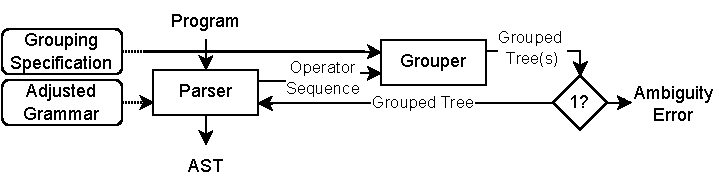
\includegraphics[scale=1.1]{figures/Approach_Overview.pdf} \pause

  \vfill
  \raggedright
  Conventional parser, new \emph{grouper} \pause

  \vfill
  Operator sequence(s)

  \vfill
  \centering
  \begin{tikzpicture}[node distance=5pt]
    \tikzset{code/.style={inner sep=3pt,outer sep=auto}}
    \tikzset{item marker/.style={circle,inner sep=2pt,draw,fill=black}}
    \node[code] (if) {\code{if}};
    \node[code,right=of if] (a) {\code{a}};
    \node[code,right=of a] (or) {\code{||}};
    \node[code,right=of or] (b) {\code{b}};
    \node[code,right=of b] (then) {\code{then}};
    \node[code,right=of then] (x) {\code{x}};
    \node[code,right=of x] (else) {\code{else}};
    \node[code,right=of else] (y) {\code{y}};

    \begin{scope}[on background layer={color = light gray}]
      \node[fit=(if) (y),fill,inner sep=0pt] {};
    \end{scope}

    \coordinate[above=of if] (above);
    \coordinate[below=of if] (below);

    \onslide<4->{
    \node[item marker] (item1) at ({$(if.west)!0.5!(then.east)$} |- above) {};
    \draw
      (if.west) |- (item1)
      (then.east) |- (item1)
    ;
    \node[item marker] (item2) at ({$(x.west)!0.5!(x.east)$} |- above) {};
    \draw
      (x.west) |- (item2)
      (x.east) |- (item2)
    ;
    \node[item marker] (item3) at ({$(else.west)!0.5!(else.east)$} |- above) {};
    \draw
      (else.west) |- (item3)
      (else.east) |- (item3)
    ;
    \node[item marker] (item4) at ({$(y.west)!0.5!(y.east)$} |- above) {};
    \draw
      (y.west) |- (item4)
      (y.east) |- (item4)
    ;
    }
    \onslide<5->{
    \node[item marker] (item5) at ({$(a.west)!0.5!(a.east)$} |- below) {};
    \draw
      (a.west) |- (item5)
      (a.east) |- (item5)
    ;
    \node[item marker] (item6) at ({$(or.west)!0.5!(or.east)$} |- below) {};
    \draw
      (or.west) |- (item6)
      (or.east) |- (item6)
    ;
    \node[item marker] (item7) at ({$(b.west)!0.5!(b.east)$} |- below) {};
    \draw
      (b.west) |- (item7)
      (b.east) |- (item7)
    ;
    }
  \end{tikzpicture}
\end{frame}

\begin{frame}{\textbf{C5:} Evaluating Performance and Expressivity \hfill \textbf{R2}, \textbf{P3}}
  Modify \code{ocamlc} to use our approach for expressions \pause

  \vfill
  Parse $\sim$\num{1000000} files spread over \num{1533} packages in Opam \pause

  \vfill
  \centering
  \resizebox{0.75\textwidth}{!}{\clipbox{0pt 0pt 0pt 30pt}{%% Creator: Matplotlib, PGF backend
%%
%% To include the figure in your LaTeX document, write
%%   \input{<filename>.pgf}
%%
%% Make sure the required packages are loaded in your preamble
%%   \usepackage{pgf}
%%
%% Also ensure that all the required font packages are loaded; for instance,
%% the lmodern package is sometimes necessary when using math font.
%%   \usepackage{lmodern}
%%
%% Figures using additional raster images can only be included by \input if
%% they are in the same directory as the main LaTeX file. For loading figures
%% from other directories you can use the `import` package
%%   \usepackage{import}
%%
%% and then include the figures with
%%   \import{<path to file>}{<filename>.pgf}
%%
%% Matplotlib used the following preamble
%%   \usepackage{fontspec}
%%   \setmainfont{DejaVuSerif.ttf}[Path=\detokenize{/home/vipa/.local/lib/python3.8/site-packages/matplotlib/mpl-data/fonts/ttf/}]
%%   \setsansfont{DejaVuSans.ttf}[Path=\detokenize{/home/vipa/.local/lib/python3.8/site-packages/matplotlib/mpl-data/fonts/ttf/}]
%%   \setmonofont{DejaVuSansMono.ttf}[Path=\detokenize{/home/vipa/.local/lib/python3.8/site-packages/matplotlib/mpl-data/fonts/ttf/}]
%%
\begingroup%
\makeatletter%
\begin{pgfpicture}%
\pgfpathrectangle{\pgfpointorigin}{\pgfqpoint{5.476996in}{2.500000in}}%
\pgfusepath{use as bounding box, clip}%
\begin{pgfscope}%
\pgfsetbuttcap%
\pgfsetmiterjoin%
\definecolor{currentfill}{rgb}{1.000000,1.000000,1.000000}%
\pgfsetfillcolor{currentfill}%
\pgfsetlinewidth{0.000000pt}%
\definecolor{currentstroke}{rgb}{1.000000,1.000000,1.000000}%
\pgfsetstrokecolor{currentstroke}%
\pgfsetdash{}{0pt}%
\pgfpathmoveto{\pgfqpoint{0.000000in}{0.000000in}}%
\pgfpathlineto{\pgfqpoint{5.476996in}{0.000000in}}%
\pgfpathlineto{\pgfqpoint{5.476996in}{2.500000in}}%
\pgfpathlineto{\pgfqpoint{0.000000in}{2.500000in}}%
\pgfpathlineto{\pgfqpoint{0.000000in}{0.000000in}}%
\pgfpathclose%
\pgfusepath{fill}%
\end{pgfscope}%
\begin{pgfscope}%
\pgfsetbuttcap%
\pgfsetmiterjoin%
\definecolor{currentfill}{rgb}{1.000000,1.000000,1.000000}%
\pgfsetfillcolor{currentfill}%
\pgfsetlinewidth{0.000000pt}%
\definecolor{currentstroke}{rgb}{0.000000,0.000000,0.000000}%
\pgfsetstrokecolor{currentstroke}%
\pgfsetstrokeopacity{0.000000}%
\pgfsetdash{}{0pt}%
\pgfpathmoveto{\pgfqpoint{0.967383in}{0.571603in}}%
\pgfpathlineto{\pgfqpoint{2.827996in}{0.571603in}}%
\pgfpathlineto{\pgfqpoint{2.827996in}{1.828744in}}%
\pgfpathlineto{\pgfqpoint{0.967383in}{1.828744in}}%
\pgfpathlineto{\pgfqpoint{0.967383in}{0.571603in}}%
\pgfpathclose%
\pgfusepath{fill}%
\end{pgfscope}%
\begin{pgfscope}%
\pgfpathrectangle{\pgfqpoint{0.967383in}{0.571603in}}{\pgfqpoint{1.860613in}{1.257140in}}%
\pgfusepath{clip}%
\pgfsetbuttcap%
\pgfsetmiterjoin%
\definecolor{currentfill}{rgb}{0.121569,0.466667,0.705882}%
\pgfsetfillcolor{currentfill}%
\pgfsetfillopacity{0.500000}%
\pgfsetlinewidth{0.000000pt}%
\definecolor{currentstroke}{rgb}{0.000000,0.000000,0.000000}%
\pgfsetstrokecolor{currentstroke}%
\pgfsetstrokeopacity{0.500000}%
\pgfsetdash{}{0pt}%
\pgfpathmoveto{\pgfqpoint{1.051956in}{0.571603in}}%
\pgfpathlineto{\pgfqpoint{1.068871in}{0.571603in}}%
\pgfpathlineto{\pgfqpoint{1.068871in}{0.599540in}}%
\pgfpathlineto{\pgfqpoint{1.051956in}{0.599540in}}%
\pgfpathlineto{\pgfqpoint{1.051956in}{0.571603in}}%
\pgfpathclose%
\pgfusepath{fill}%
\end{pgfscope}%
\begin{pgfscope}%
\pgfpathrectangle{\pgfqpoint{0.967383in}{0.571603in}}{\pgfqpoint{1.860613in}{1.257140in}}%
\pgfusepath{clip}%
\pgfsetbuttcap%
\pgfsetmiterjoin%
\definecolor{currentfill}{rgb}{0.121569,0.466667,0.705882}%
\pgfsetfillcolor{currentfill}%
\pgfsetfillopacity{0.500000}%
\pgfsetlinewidth{0.000000pt}%
\definecolor{currentstroke}{rgb}{0.000000,0.000000,0.000000}%
\pgfsetstrokecolor{currentstroke}%
\pgfsetstrokeopacity{0.500000}%
\pgfsetdash{}{0pt}%
\pgfpathmoveto{\pgfqpoint{1.068871in}{0.571603in}}%
\pgfpathlineto{\pgfqpoint{1.085785in}{0.571603in}}%
\pgfpathlineto{\pgfqpoint{1.085785in}{0.571603in}}%
\pgfpathlineto{\pgfqpoint{1.068871in}{0.571603in}}%
\pgfpathlineto{\pgfqpoint{1.068871in}{0.571603in}}%
\pgfpathclose%
\pgfusepath{fill}%
\end{pgfscope}%
\begin{pgfscope}%
\pgfpathrectangle{\pgfqpoint{0.967383in}{0.571603in}}{\pgfqpoint{1.860613in}{1.257140in}}%
\pgfusepath{clip}%
\pgfsetbuttcap%
\pgfsetmiterjoin%
\definecolor{currentfill}{rgb}{0.121569,0.466667,0.705882}%
\pgfsetfillcolor{currentfill}%
\pgfsetfillopacity{0.500000}%
\pgfsetlinewidth{0.000000pt}%
\definecolor{currentstroke}{rgb}{0.000000,0.000000,0.000000}%
\pgfsetstrokecolor{currentstroke}%
\pgfsetstrokeopacity{0.500000}%
\pgfsetdash{}{0pt}%
\pgfpathmoveto{\pgfqpoint{1.085785in}{0.571603in}}%
\pgfpathlineto{\pgfqpoint{1.102700in}{0.571603in}}%
\pgfpathlineto{\pgfqpoint{1.102700in}{0.571603in}}%
\pgfpathlineto{\pgfqpoint{1.085785in}{0.571603in}}%
\pgfpathlineto{\pgfqpoint{1.085785in}{0.571603in}}%
\pgfpathclose%
\pgfusepath{fill}%
\end{pgfscope}%
\begin{pgfscope}%
\pgfpathrectangle{\pgfqpoint{0.967383in}{0.571603in}}{\pgfqpoint{1.860613in}{1.257140in}}%
\pgfusepath{clip}%
\pgfsetbuttcap%
\pgfsetmiterjoin%
\definecolor{currentfill}{rgb}{0.121569,0.466667,0.705882}%
\pgfsetfillcolor{currentfill}%
\pgfsetfillopacity{0.500000}%
\pgfsetlinewidth{0.000000pt}%
\definecolor{currentstroke}{rgb}{0.000000,0.000000,0.000000}%
\pgfsetstrokecolor{currentstroke}%
\pgfsetstrokeopacity{0.500000}%
\pgfsetdash{}{0pt}%
\pgfpathmoveto{\pgfqpoint{1.102700in}{0.571603in}}%
\pgfpathlineto{\pgfqpoint{1.119615in}{0.571603in}}%
\pgfpathlineto{\pgfqpoint{1.119615in}{0.571608in}}%
\pgfpathlineto{\pgfqpoint{1.102700in}{0.571608in}}%
\pgfpathlineto{\pgfqpoint{1.102700in}{0.571603in}}%
\pgfpathclose%
\pgfusepath{fill}%
\end{pgfscope}%
\begin{pgfscope}%
\pgfpathrectangle{\pgfqpoint{0.967383in}{0.571603in}}{\pgfqpoint{1.860613in}{1.257140in}}%
\pgfusepath{clip}%
\pgfsetbuttcap%
\pgfsetmiterjoin%
\definecolor{currentfill}{rgb}{0.121569,0.466667,0.705882}%
\pgfsetfillcolor{currentfill}%
\pgfsetfillopacity{0.500000}%
\pgfsetlinewidth{0.000000pt}%
\definecolor{currentstroke}{rgb}{0.000000,0.000000,0.000000}%
\pgfsetstrokecolor{currentstroke}%
\pgfsetstrokeopacity{0.500000}%
\pgfsetdash{}{0pt}%
\pgfpathmoveto{\pgfqpoint{1.119615in}{0.571603in}}%
\pgfpathlineto{\pgfqpoint{1.136529in}{0.571603in}}%
\pgfpathlineto{\pgfqpoint{1.136529in}{0.571719in}}%
\pgfpathlineto{\pgfqpoint{1.119615in}{0.571719in}}%
\pgfpathlineto{\pgfqpoint{1.119615in}{0.571603in}}%
\pgfpathclose%
\pgfusepath{fill}%
\end{pgfscope}%
\begin{pgfscope}%
\pgfpathrectangle{\pgfqpoint{0.967383in}{0.571603in}}{\pgfqpoint{1.860613in}{1.257140in}}%
\pgfusepath{clip}%
\pgfsetbuttcap%
\pgfsetmiterjoin%
\definecolor{currentfill}{rgb}{0.121569,0.466667,0.705882}%
\pgfsetfillcolor{currentfill}%
\pgfsetfillopacity{0.500000}%
\pgfsetlinewidth{0.000000pt}%
\definecolor{currentstroke}{rgb}{0.000000,0.000000,0.000000}%
\pgfsetstrokecolor{currentstroke}%
\pgfsetstrokeopacity{0.500000}%
\pgfsetdash{}{0pt}%
\pgfpathmoveto{\pgfqpoint{1.136529in}{0.571603in}}%
\pgfpathlineto{\pgfqpoint{1.153444in}{0.571603in}}%
\pgfpathlineto{\pgfqpoint{1.153444in}{0.571909in}}%
\pgfpathlineto{\pgfqpoint{1.136529in}{0.571909in}}%
\pgfpathlineto{\pgfqpoint{1.136529in}{0.571603in}}%
\pgfpathclose%
\pgfusepath{fill}%
\end{pgfscope}%
\begin{pgfscope}%
\pgfpathrectangle{\pgfqpoint{0.967383in}{0.571603in}}{\pgfqpoint{1.860613in}{1.257140in}}%
\pgfusepath{clip}%
\pgfsetbuttcap%
\pgfsetmiterjoin%
\definecolor{currentfill}{rgb}{0.121569,0.466667,0.705882}%
\pgfsetfillcolor{currentfill}%
\pgfsetfillopacity{0.500000}%
\pgfsetlinewidth{0.000000pt}%
\definecolor{currentstroke}{rgb}{0.000000,0.000000,0.000000}%
\pgfsetstrokecolor{currentstroke}%
\pgfsetstrokeopacity{0.500000}%
\pgfsetdash{}{0pt}%
\pgfpathmoveto{\pgfqpoint{1.153444in}{0.571603in}}%
\pgfpathlineto{\pgfqpoint{1.170359in}{0.571603in}}%
\pgfpathlineto{\pgfqpoint{1.170359in}{0.572256in}}%
\pgfpathlineto{\pgfqpoint{1.153444in}{0.572256in}}%
\pgfpathlineto{\pgfqpoint{1.153444in}{0.571603in}}%
\pgfpathclose%
\pgfusepath{fill}%
\end{pgfscope}%
\begin{pgfscope}%
\pgfpathrectangle{\pgfqpoint{0.967383in}{0.571603in}}{\pgfqpoint{1.860613in}{1.257140in}}%
\pgfusepath{clip}%
\pgfsetbuttcap%
\pgfsetmiterjoin%
\definecolor{currentfill}{rgb}{0.121569,0.466667,0.705882}%
\pgfsetfillcolor{currentfill}%
\pgfsetfillopacity{0.500000}%
\pgfsetlinewidth{0.000000pt}%
\definecolor{currentstroke}{rgb}{0.000000,0.000000,0.000000}%
\pgfsetstrokecolor{currentstroke}%
\pgfsetstrokeopacity{0.500000}%
\pgfsetdash{}{0pt}%
\pgfpathmoveto{\pgfqpoint{1.170359in}{0.571603in}}%
\pgfpathlineto{\pgfqpoint{1.187273in}{0.571603in}}%
\pgfpathlineto{\pgfqpoint{1.187273in}{0.571769in}}%
\pgfpathlineto{\pgfqpoint{1.170359in}{0.571769in}}%
\pgfpathlineto{\pgfqpoint{1.170359in}{0.571603in}}%
\pgfpathclose%
\pgfusepath{fill}%
\end{pgfscope}%
\begin{pgfscope}%
\pgfpathrectangle{\pgfqpoint{0.967383in}{0.571603in}}{\pgfqpoint{1.860613in}{1.257140in}}%
\pgfusepath{clip}%
\pgfsetbuttcap%
\pgfsetmiterjoin%
\definecolor{currentfill}{rgb}{0.121569,0.466667,0.705882}%
\pgfsetfillcolor{currentfill}%
\pgfsetfillopacity{0.500000}%
\pgfsetlinewidth{0.000000pt}%
\definecolor{currentstroke}{rgb}{0.000000,0.000000,0.000000}%
\pgfsetstrokecolor{currentstroke}%
\pgfsetstrokeopacity{0.500000}%
\pgfsetdash{}{0pt}%
\pgfpathmoveto{\pgfqpoint{1.187273in}{0.571603in}}%
\pgfpathlineto{\pgfqpoint{1.204188in}{0.571603in}}%
\pgfpathlineto{\pgfqpoint{1.204188in}{0.573786in}}%
\pgfpathlineto{\pgfqpoint{1.187273in}{0.573786in}}%
\pgfpathlineto{\pgfqpoint{1.187273in}{0.571603in}}%
\pgfpathclose%
\pgfusepath{fill}%
\end{pgfscope}%
\begin{pgfscope}%
\pgfpathrectangle{\pgfqpoint{0.967383in}{0.571603in}}{\pgfqpoint{1.860613in}{1.257140in}}%
\pgfusepath{clip}%
\pgfsetbuttcap%
\pgfsetmiterjoin%
\definecolor{currentfill}{rgb}{0.121569,0.466667,0.705882}%
\pgfsetfillcolor{currentfill}%
\pgfsetfillopacity{0.500000}%
\pgfsetlinewidth{0.000000pt}%
\definecolor{currentstroke}{rgb}{0.000000,0.000000,0.000000}%
\pgfsetstrokecolor{currentstroke}%
\pgfsetstrokeopacity{0.500000}%
\pgfsetdash{}{0pt}%
\pgfpathmoveto{\pgfqpoint{1.204188in}{0.571603in}}%
\pgfpathlineto{\pgfqpoint{1.221103in}{0.571603in}}%
\pgfpathlineto{\pgfqpoint{1.221103in}{0.571834in}}%
\pgfpathlineto{\pgfqpoint{1.204188in}{0.571834in}}%
\pgfpathlineto{\pgfqpoint{1.204188in}{0.571603in}}%
\pgfpathclose%
\pgfusepath{fill}%
\end{pgfscope}%
\begin{pgfscope}%
\pgfpathrectangle{\pgfqpoint{0.967383in}{0.571603in}}{\pgfqpoint{1.860613in}{1.257140in}}%
\pgfusepath{clip}%
\pgfsetbuttcap%
\pgfsetmiterjoin%
\definecolor{currentfill}{rgb}{0.121569,0.466667,0.705882}%
\pgfsetfillcolor{currentfill}%
\pgfsetfillopacity{0.500000}%
\pgfsetlinewidth{0.000000pt}%
\definecolor{currentstroke}{rgb}{0.000000,0.000000,0.000000}%
\pgfsetstrokecolor{currentstroke}%
\pgfsetstrokeopacity{0.500000}%
\pgfsetdash{}{0pt}%
\pgfpathmoveto{\pgfqpoint{1.221103in}{0.571603in}}%
\pgfpathlineto{\pgfqpoint{1.238017in}{0.571603in}}%
\pgfpathlineto{\pgfqpoint{1.238017in}{0.572206in}}%
\pgfpathlineto{\pgfqpoint{1.221103in}{0.572206in}}%
\pgfpathlineto{\pgfqpoint{1.221103in}{0.571603in}}%
\pgfpathclose%
\pgfusepath{fill}%
\end{pgfscope}%
\begin{pgfscope}%
\pgfpathrectangle{\pgfqpoint{0.967383in}{0.571603in}}{\pgfqpoint{1.860613in}{1.257140in}}%
\pgfusepath{clip}%
\pgfsetbuttcap%
\pgfsetmiterjoin%
\definecolor{currentfill}{rgb}{0.121569,0.466667,0.705882}%
\pgfsetfillcolor{currentfill}%
\pgfsetfillopacity{0.500000}%
\pgfsetlinewidth{0.000000pt}%
\definecolor{currentstroke}{rgb}{0.000000,0.000000,0.000000}%
\pgfsetstrokecolor{currentstroke}%
\pgfsetstrokeopacity{0.500000}%
\pgfsetdash{}{0pt}%
\pgfpathmoveto{\pgfqpoint{1.238017in}{0.571603in}}%
\pgfpathlineto{\pgfqpoint{1.254932in}{0.571603in}}%
\pgfpathlineto{\pgfqpoint{1.254932in}{0.580998in}}%
\pgfpathlineto{\pgfqpoint{1.238017in}{0.580998in}}%
\pgfpathlineto{\pgfqpoint{1.238017in}{0.571603in}}%
\pgfpathclose%
\pgfusepath{fill}%
\end{pgfscope}%
\begin{pgfscope}%
\pgfpathrectangle{\pgfqpoint{0.967383in}{0.571603in}}{\pgfqpoint{1.860613in}{1.257140in}}%
\pgfusepath{clip}%
\pgfsetbuttcap%
\pgfsetmiterjoin%
\definecolor{currentfill}{rgb}{0.121569,0.466667,0.705882}%
\pgfsetfillcolor{currentfill}%
\pgfsetfillopacity{0.500000}%
\pgfsetlinewidth{0.000000pt}%
\definecolor{currentstroke}{rgb}{0.000000,0.000000,0.000000}%
\pgfsetstrokecolor{currentstroke}%
\pgfsetstrokeopacity{0.500000}%
\pgfsetdash{}{0pt}%
\pgfpathmoveto{\pgfqpoint{1.254932in}{0.571603in}}%
\pgfpathlineto{\pgfqpoint{1.271847in}{0.571603in}}%
\pgfpathlineto{\pgfqpoint{1.271847in}{0.573801in}}%
\pgfpathlineto{\pgfqpoint{1.254932in}{0.573801in}}%
\pgfpathlineto{\pgfqpoint{1.254932in}{0.571603in}}%
\pgfpathclose%
\pgfusepath{fill}%
\end{pgfscope}%
\begin{pgfscope}%
\pgfpathrectangle{\pgfqpoint{0.967383in}{0.571603in}}{\pgfqpoint{1.860613in}{1.257140in}}%
\pgfusepath{clip}%
\pgfsetbuttcap%
\pgfsetmiterjoin%
\definecolor{currentfill}{rgb}{0.121569,0.466667,0.705882}%
\pgfsetfillcolor{currentfill}%
\pgfsetfillopacity{0.500000}%
\pgfsetlinewidth{0.000000pt}%
\definecolor{currentstroke}{rgb}{0.000000,0.000000,0.000000}%
\pgfsetstrokecolor{currentstroke}%
\pgfsetstrokeopacity{0.500000}%
\pgfsetdash{}{0pt}%
\pgfpathmoveto{\pgfqpoint{1.271847in}{0.571603in}}%
\pgfpathlineto{\pgfqpoint{1.288761in}{0.571603in}}%
\pgfpathlineto{\pgfqpoint{1.288761in}{0.574439in}}%
\pgfpathlineto{\pgfqpoint{1.271847in}{0.574439in}}%
\pgfpathlineto{\pgfqpoint{1.271847in}{0.571603in}}%
\pgfpathclose%
\pgfusepath{fill}%
\end{pgfscope}%
\begin{pgfscope}%
\pgfpathrectangle{\pgfqpoint{0.967383in}{0.571603in}}{\pgfqpoint{1.860613in}{1.257140in}}%
\pgfusepath{clip}%
\pgfsetbuttcap%
\pgfsetmiterjoin%
\definecolor{currentfill}{rgb}{0.121569,0.466667,0.705882}%
\pgfsetfillcolor{currentfill}%
\pgfsetfillopacity{0.500000}%
\pgfsetlinewidth{0.000000pt}%
\definecolor{currentstroke}{rgb}{0.000000,0.000000,0.000000}%
\pgfsetstrokecolor{currentstroke}%
\pgfsetstrokeopacity{0.500000}%
\pgfsetdash{}{0pt}%
\pgfpathmoveto{\pgfqpoint{1.288761in}{0.571603in}}%
\pgfpathlineto{\pgfqpoint{1.305676in}{0.571603in}}%
\pgfpathlineto{\pgfqpoint{1.305676in}{0.574298in}}%
\pgfpathlineto{\pgfqpoint{1.288761in}{0.574298in}}%
\pgfpathlineto{\pgfqpoint{1.288761in}{0.571603in}}%
\pgfpathclose%
\pgfusepath{fill}%
\end{pgfscope}%
\begin{pgfscope}%
\pgfpathrectangle{\pgfqpoint{0.967383in}{0.571603in}}{\pgfqpoint{1.860613in}{1.257140in}}%
\pgfusepath{clip}%
\pgfsetbuttcap%
\pgfsetmiterjoin%
\definecolor{currentfill}{rgb}{0.121569,0.466667,0.705882}%
\pgfsetfillcolor{currentfill}%
\pgfsetfillopacity{0.500000}%
\pgfsetlinewidth{0.000000pt}%
\definecolor{currentstroke}{rgb}{0.000000,0.000000,0.000000}%
\pgfsetstrokecolor{currentstroke}%
\pgfsetstrokeopacity{0.500000}%
\pgfsetdash{}{0pt}%
\pgfpathmoveto{\pgfqpoint{1.305676in}{0.571603in}}%
\pgfpathlineto{\pgfqpoint{1.322591in}{0.571603in}}%
\pgfpathlineto{\pgfqpoint{1.322591in}{0.573234in}}%
\pgfpathlineto{\pgfqpoint{1.305676in}{0.573234in}}%
\pgfpathlineto{\pgfqpoint{1.305676in}{0.571603in}}%
\pgfpathclose%
\pgfusepath{fill}%
\end{pgfscope}%
\begin{pgfscope}%
\pgfpathrectangle{\pgfqpoint{0.967383in}{0.571603in}}{\pgfqpoint{1.860613in}{1.257140in}}%
\pgfusepath{clip}%
\pgfsetbuttcap%
\pgfsetmiterjoin%
\definecolor{currentfill}{rgb}{0.121569,0.466667,0.705882}%
\pgfsetfillcolor{currentfill}%
\pgfsetfillopacity{0.500000}%
\pgfsetlinewidth{0.000000pt}%
\definecolor{currentstroke}{rgb}{0.000000,0.000000,0.000000}%
\pgfsetstrokecolor{currentstroke}%
\pgfsetstrokeopacity{0.500000}%
\pgfsetdash{}{0pt}%
\pgfpathmoveto{\pgfqpoint{1.322591in}{0.571603in}}%
\pgfpathlineto{\pgfqpoint{1.339505in}{0.571603in}}%
\pgfpathlineto{\pgfqpoint{1.339505in}{1.768880in}}%
\pgfpathlineto{\pgfqpoint{1.322591in}{1.768880in}}%
\pgfpathlineto{\pgfqpoint{1.322591in}{0.571603in}}%
\pgfpathclose%
\pgfusepath{fill}%
\end{pgfscope}%
\begin{pgfscope}%
\pgfpathrectangle{\pgfqpoint{0.967383in}{0.571603in}}{\pgfqpoint{1.860613in}{1.257140in}}%
\pgfusepath{clip}%
\pgfsetbuttcap%
\pgfsetmiterjoin%
\definecolor{currentfill}{rgb}{0.121569,0.466667,0.705882}%
\pgfsetfillcolor{currentfill}%
\pgfsetfillopacity{0.500000}%
\pgfsetlinewidth{0.000000pt}%
\definecolor{currentstroke}{rgb}{0.000000,0.000000,0.000000}%
\pgfsetstrokecolor{currentstroke}%
\pgfsetstrokeopacity{0.500000}%
\pgfsetdash{}{0pt}%
\pgfpathmoveto{\pgfqpoint{1.339505in}{0.571603in}}%
\pgfpathlineto{\pgfqpoint{1.356420in}{0.571603in}}%
\pgfpathlineto{\pgfqpoint{1.356420in}{0.575006in}}%
\pgfpathlineto{\pgfqpoint{1.339505in}{0.575006in}}%
\pgfpathlineto{\pgfqpoint{1.339505in}{0.571603in}}%
\pgfpathclose%
\pgfusepath{fill}%
\end{pgfscope}%
\begin{pgfscope}%
\pgfpathrectangle{\pgfqpoint{0.967383in}{0.571603in}}{\pgfqpoint{1.860613in}{1.257140in}}%
\pgfusepath{clip}%
\pgfsetbuttcap%
\pgfsetmiterjoin%
\definecolor{currentfill}{rgb}{0.121569,0.466667,0.705882}%
\pgfsetfillcolor{currentfill}%
\pgfsetfillopacity{0.500000}%
\pgfsetlinewidth{0.000000pt}%
\definecolor{currentstroke}{rgb}{0.000000,0.000000,0.000000}%
\pgfsetstrokecolor{currentstroke}%
\pgfsetstrokeopacity{0.500000}%
\pgfsetdash{}{0pt}%
\pgfpathmoveto{\pgfqpoint{1.356420in}{0.571603in}}%
\pgfpathlineto{\pgfqpoint{1.373335in}{0.571603in}}%
\pgfpathlineto{\pgfqpoint{1.373335in}{0.575979in}}%
\pgfpathlineto{\pgfqpoint{1.356420in}{0.575979in}}%
\pgfpathlineto{\pgfqpoint{1.356420in}{0.571603in}}%
\pgfpathclose%
\pgfusepath{fill}%
\end{pgfscope}%
\begin{pgfscope}%
\pgfpathrectangle{\pgfqpoint{0.967383in}{0.571603in}}{\pgfqpoint{1.860613in}{1.257140in}}%
\pgfusepath{clip}%
\pgfsetbuttcap%
\pgfsetmiterjoin%
\definecolor{currentfill}{rgb}{0.121569,0.466667,0.705882}%
\pgfsetfillcolor{currentfill}%
\pgfsetfillopacity{0.500000}%
\pgfsetlinewidth{0.000000pt}%
\definecolor{currentstroke}{rgb}{0.000000,0.000000,0.000000}%
\pgfsetstrokecolor{currentstroke}%
\pgfsetstrokeopacity{0.500000}%
\pgfsetdash{}{0pt}%
\pgfpathmoveto{\pgfqpoint{1.373335in}{0.571603in}}%
\pgfpathlineto{\pgfqpoint{1.390249in}{0.571603in}}%
\pgfpathlineto{\pgfqpoint{1.390249in}{0.597327in}}%
\pgfpathlineto{\pgfqpoint{1.373335in}{0.597327in}}%
\pgfpathlineto{\pgfqpoint{1.373335in}{0.571603in}}%
\pgfpathclose%
\pgfusepath{fill}%
\end{pgfscope}%
\begin{pgfscope}%
\pgfpathrectangle{\pgfqpoint{0.967383in}{0.571603in}}{\pgfqpoint{1.860613in}{1.257140in}}%
\pgfusepath{clip}%
\pgfsetbuttcap%
\pgfsetmiterjoin%
\definecolor{currentfill}{rgb}{0.121569,0.466667,0.705882}%
\pgfsetfillcolor{currentfill}%
\pgfsetfillopacity{0.500000}%
\pgfsetlinewidth{0.000000pt}%
\definecolor{currentstroke}{rgb}{0.000000,0.000000,0.000000}%
\pgfsetstrokecolor{currentstroke}%
\pgfsetstrokeopacity{0.500000}%
\pgfsetdash{}{0pt}%
\pgfpathmoveto{\pgfqpoint{1.390249in}{0.571603in}}%
\pgfpathlineto{\pgfqpoint{1.407164in}{0.571603in}}%
\pgfpathlineto{\pgfqpoint{1.407164in}{0.615925in}}%
\pgfpathlineto{\pgfqpoint{1.390249in}{0.615925in}}%
\pgfpathlineto{\pgfqpoint{1.390249in}{0.571603in}}%
\pgfpathclose%
\pgfusepath{fill}%
\end{pgfscope}%
\begin{pgfscope}%
\pgfpathrectangle{\pgfqpoint{0.967383in}{0.571603in}}{\pgfqpoint{1.860613in}{1.257140in}}%
\pgfusepath{clip}%
\pgfsetbuttcap%
\pgfsetmiterjoin%
\definecolor{currentfill}{rgb}{0.121569,0.466667,0.705882}%
\pgfsetfillcolor{currentfill}%
\pgfsetfillopacity{0.500000}%
\pgfsetlinewidth{0.000000pt}%
\definecolor{currentstroke}{rgb}{0.000000,0.000000,0.000000}%
\pgfsetstrokecolor{currentstroke}%
\pgfsetstrokeopacity{0.500000}%
\pgfsetdash{}{0pt}%
\pgfpathmoveto{\pgfqpoint{1.407164in}{0.571603in}}%
\pgfpathlineto{\pgfqpoint{1.424079in}{0.571603in}}%
\pgfpathlineto{\pgfqpoint{1.424079in}{0.588169in}}%
\pgfpathlineto{\pgfqpoint{1.407164in}{0.588169in}}%
\pgfpathlineto{\pgfqpoint{1.407164in}{0.571603in}}%
\pgfpathclose%
\pgfusepath{fill}%
\end{pgfscope}%
\begin{pgfscope}%
\pgfpathrectangle{\pgfqpoint{0.967383in}{0.571603in}}{\pgfqpoint{1.860613in}{1.257140in}}%
\pgfusepath{clip}%
\pgfsetbuttcap%
\pgfsetmiterjoin%
\definecolor{currentfill}{rgb}{0.121569,0.466667,0.705882}%
\pgfsetfillcolor{currentfill}%
\pgfsetfillopacity{0.500000}%
\pgfsetlinewidth{0.000000pt}%
\definecolor{currentstroke}{rgb}{0.000000,0.000000,0.000000}%
\pgfsetstrokecolor{currentstroke}%
\pgfsetstrokeopacity{0.500000}%
\pgfsetdash{}{0pt}%
\pgfpathmoveto{\pgfqpoint{1.424079in}{0.571603in}}%
\pgfpathlineto{\pgfqpoint{1.440993in}{0.571603in}}%
\pgfpathlineto{\pgfqpoint{1.440993in}{0.754259in}}%
\pgfpathlineto{\pgfqpoint{1.424079in}{0.754259in}}%
\pgfpathlineto{\pgfqpoint{1.424079in}{0.571603in}}%
\pgfpathclose%
\pgfusepath{fill}%
\end{pgfscope}%
\begin{pgfscope}%
\pgfpathrectangle{\pgfqpoint{0.967383in}{0.571603in}}{\pgfqpoint{1.860613in}{1.257140in}}%
\pgfusepath{clip}%
\pgfsetbuttcap%
\pgfsetmiterjoin%
\definecolor{currentfill}{rgb}{0.121569,0.466667,0.705882}%
\pgfsetfillcolor{currentfill}%
\pgfsetfillopacity{0.500000}%
\pgfsetlinewidth{0.000000pt}%
\definecolor{currentstroke}{rgb}{0.000000,0.000000,0.000000}%
\pgfsetstrokecolor{currentstroke}%
\pgfsetstrokeopacity{0.500000}%
\pgfsetdash{}{0pt}%
\pgfpathmoveto{\pgfqpoint{1.440993in}{0.571603in}}%
\pgfpathlineto{\pgfqpoint{1.457908in}{0.571603in}}%
\pgfpathlineto{\pgfqpoint{1.457908in}{0.636284in}}%
\pgfpathlineto{\pgfqpoint{1.440993in}{0.636284in}}%
\pgfpathlineto{\pgfqpoint{1.440993in}{0.571603in}}%
\pgfpathclose%
\pgfusepath{fill}%
\end{pgfscope}%
\begin{pgfscope}%
\pgfpathrectangle{\pgfqpoint{0.967383in}{0.571603in}}{\pgfqpoint{1.860613in}{1.257140in}}%
\pgfusepath{clip}%
\pgfsetbuttcap%
\pgfsetmiterjoin%
\definecolor{currentfill}{rgb}{0.121569,0.466667,0.705882}%
\pgfsetfillcolor{currentfill}%
\pgfsetfillopacity{0.500000}%
\pgfsetlinewidth{0.000000pt}%
\definecolor{currentstroke}{rgb}{0.000000,0.000000,0.000000}%
\pgfsetstrokecolor{currentstroke}%
\pgfsetstrokeopacity{0.500000}%
\pgfsetdash{}{0pt}%
\pgfpathmoveto{\pgfqpoint{1.457908in}{0.571603in}}%
\pgfpathlineto{\pgfqpoint{1.474823in}{0.571603in}}%
\pgfpathlineto{\pgfqpoint{1.474823in}{0.597568in}}%
\pgfpathlineto{\pgfqpoint{1.457908in}{0.597568in}}%
\pgfpathlineto{\pgfqpoint{1.457908in}{0.571603in}}%
\pgfpathclose%
\pgfusepath{fill}%
\end{pgfscope}%
\begin{pgfscope}%
\pgfpathrectangle{\pgfqpoint{0.967383in}{0.571603in}}{\pgfqpoint{1.860613in}{1.257140in}}%
\pgfusepath{clip}%
\pgfsetbuttcap%
\pgfsetmiterjoin%
\definecolor{currentfill}{rgb}{0.121569,0.466667,0.705882}%
\pgfsetfillcolor{currentfill}%
\pgfsetfillopacity{0.500000}%
\pgfsetlinewidth{0.000000pt}%
\definecolor{currentstroke}{rgb}{0.000000,0.000000,0.000000}%
\pgfsetstrokecolor{currentstroke}%
\pgfsetstrokeopacity{0.500000}%
\pgfsetdash{}{0pt}%
\pgfpathmoveto{\pgfqpoint{1.474823in}{0.571603in}}%
\pgfpathlineto{\pgfqpoint{1.491737in}{0.571603in}}%
\pgfpathlineto{\pgfqpoint{1.491737in}{0.930165in}}%
\pgfpathlineto{\pgfqpoint{1.474823in}{0.930165in}}%
\pgfpathlineto{\pgfqpoint{1.474823in}{0.571603in}}%
\pgfpathclose%
\pgfusepath{fill}%
\end{pgfscope}%
\begin{pgfscope}%
\pgfpathrectangle{\pgfqpoint{0.967383in}{0.571603in}}{\pgfqpoint{1.860613in}{1.257140in}}%
\pgfusepath{clip}%
\pgfsetbuttcap%
\pgfsetmiterjoin%
\definecolor{currentfill}{rgb}{0.121569,0.466667,0.705882}%
\pgfsetfillcolor{currentfill}%
\pgfsetfillopacity{0.500000}%
\pgfsetlinewidth{0.000000pt}%
\definecolor{currentstroke}{rgb}{0.000000,0.000000,0.000000}%
\pgfsetstrokecolor{currentstroke}%
\pgfsetstrokeopacity{0.500000}%
\pgfsetdash{}{0pt}%
\pgfpathmoveto{\pgfqpoint{1.491737in}{0.571603in}}%
\pgfpathlineto{\pgfqpoint{1.508652in}{0.571603in}}%
\pgfpathlineto{\pgfqpoint{1.508652in}{0.611087in}}%
\pgfpathlineto{\pgfqpoint{1.491737in}{0.611087in}}%
\pgfpathlineto{\pgfqpoint{1.491737in}{0.571603in}}%
\pgfpathclose%
\pgfusepath{fill}%
\end{pgfscope}%
\begin{pgfscope}%
\pgfpathrectangle{\pgfqpoint{0.967383in}{0.571603in}}{\pgfqpoint{1.860613in}{1.257140in}}%
\pgfusepath{clip}%
\pgfsetbuttcap%
\pgfsetmiterjoin%
\definecolor{currentfill}{rgb}{0.121569,0.466667,0.705882}%
\pgfsetfillcolor{currentfill}%
\pgfsetfillopacity{0.500000}%
\pgfsetlinewidth{0.000000pt}%
\definecolor{currentstroke}{rgb}{0.000000,0.000000,0.000000}%
\pgfsetstrokecolor{currentstroke}%
\pgfsetstrokeopacity{0.500000}%
\pgfsetdash{}{0pt}%
\pgfpathmoveto{\pgfqpoint{1.508652in}{0.571603in}}%
\pgfpathlineto{\pgfqpoint{1.525567in}{0.571603in}}%
\pgfpathlineto{\pgfqpoint{1.525567in}{0.724932in}}%
\pgfpathlineto{\pgfqpoint{1.508652in}{0.724932in}}%
\pgfpathlineto{\pgfqpoint{1.508652in}{0.571603in}}%
\pgfpathclose%
\pgfusepath{fill}%
\end{pgfscope}%
\begin{pgfscope}%
\pgfpathrectangle{\pgfqpoint{0.967383in}{0.571603in}}{\pgfqpoint{1.860613in}{1.257140in}}%
\pgfusepath{clip}%
\pgfsetbuttcap%
\pgfsetmiterjoin%
\definecolor{currentfill}{rgb}{0.121569,0.466667,0.705882}%
\pgfsetfillcolor{currentfill}%
\pgfsetfillopacity{0.500000}%
\pgfsetlinewidth{0.000000pt}%
\definecolor{currentstroke}{rgb}{0.000000,0.000000,0.000000}%
\pgfsetstrokecolor{currentstroke}%
\pgfsetstrokeopacity{0.500000}%
\pgfsetdash{}{0pt}%
\pgfpathmoveto{\pgfqpoint{1.525567in}{0.571603in}}%
\pgfpathlineto{\pgfqpoint{1.542481in}{0.571603in}}%
\pgfpathlineto{\pgfqpoint{1.542481in}{0.584485in}}%
\pgfpathlineto{\pgfqpoint{1.525567in}{0.584485in}}%
\pgfpathlineto{\pgfqpoint{1.525567in}{0.571603in}}%
\pgfpathclose%
\pgfusepath{fill}%
\end{pgfscope}%
\begin{pgfscope}%
\pgfpathrectangle{\pgfqpoint{0.967383in}{0.571603in}}{\pgfqpoint{1.860613in}{1.257140in}}%
\pgfusepath{clip}%
\pgfsetbuttcap%
\pgfsetmiterjoin%
\definecolor{currentfill}{rgb}{0.121569,0.466667,0.705882}%
\pgfsetfillcolor{currentfill}%
\pgfsetfillopacity{0.500000}%
\pgfsetlinewidth{0.000000pt}%
\definecolor{currentstroke}{rgb}{0.000000,0.000000,0.000000}%
\pgfsetstrokecolor{currentstroke}%
\pgfsetstrokeopacity{0.500000}%
\pgfsetdash{}{0pt}%
\pgfpathmoveto{\pgfqpoint{1.542481in}{0.571603in}}%
\pgfpathlineto{\pgfqpoint{1.559396in}{0.571603in}}%
\pgfpathlineto{\pgfqpoint{1.559396in}{0.609843in}}%
\pgfpathlineto{\pgfqpoint{1.542481in}{0.609843in}}%
\pgfpathlineto{\pgfqpoint{1.542481in}{0.571603in}}%
\pgfpathclose%
\pgfusepath{fill}%
\end{pgfscope}%
\begin{pgfscope}%
\pgfpathrectangle{\pgfqpoint{0.967383in}{0.571603in}}{\pgfqpoint{1.860613in}{1.257140in}}%
\pgfusepath{clip}%
\pgfsetbuttcap%
\pgfsetmiterjoin%
\definecolor{currentfill}{rgb}{0.121569,0.466667,0.705882}%
\pgfsetfillcolor{currentfill}%
\pgfsetfillopacity{0.500000}%
\pgfsetlinewidth{0.000000pt}%
\definecolor{currentstroke}{rgb}{0.000000,0.000000,0.000000}%
\pgfsetstrokecolor{currentstroke}%
\pgfsetstrokeopacity{0.500000}%
\pgfsetdash{}{0pt}%
\pgfpathmoveto{\pgfqpoint{1.559396in}{0.571603in}}%
\pgfpathlineto{\pgfqpoint{1.576311in}{0.571603in}}%
\pgfpathlineto{\pgfqpoint{1.576311in}{0.581304in}}%
\pgfpathlineto{\pgfqpoint{1.559396in}{0.581304in}}%
\pgfpathlineto{\pgfqpoint{1.559396in}{0.571603in}}%
\pgfpathclose%
\pgfusepath{fill}%
\end{pgfscope}%
\begin{pgfscope}%
\pgfpathrectangle{\pgfqpoint{0.967383in}{0.571603in}}{\pgfqpoint{1.860613in}{1.257140in}}%
\pgfusepath{clip}%
\pgfsetbuttcap%
\pgfsetmiterjoin%
\definecolor{currentfill}{rgb}{0.121569,0.466667,0.705882}%
\pgfsetfillcolor{currentfill}%
\pgfsetfillopacity{0.500000}%
\pgfsetlinewidth{0.000000pt}%
\definecolor{currentstroke}{rgb}{0.000000,0.000000,0.000000}%
\pgfsetstrokecolor{currentstroke}%
\pgfsetstrokeopacity{0.500000}%
\pgfsetdash{}{0pt}%
\pgfpathmoveto{\pgfqpoint{1.576311in}{0.571603in}}%
\pgfpathlineto{\pgfqpoint{1.593225in}{0.571603in}}%
\pgfpathlineto{\pgfqpoint{1.593225in}{0.573877in}}%
\pgfpathlineto{\pgfqpoint{1.576311in}{0.573877in}}%
\pgfpathlineto{\pgfqpoint{1.576311in}{0.571603in}}%
\pgfpathclose%
\pgfusepath{fill}%
\end{pgfscope}%
\begin{pgfscope}%
\pgfpathrectangle{\pgfqpoint{0.967383in}{0.571603in}}{\pgfqpoint{1.860613in}{1.257140in}}%
\pgfusepath{clip}%
\pgfsetbuttcap%
\pgfsetmiterjoin%
\definecolor{currentfill}{rgb}{0.121569,0.466667,0.705882}%
\pgfsetfillcolor{currentfill}%
\pgfsetfillopacity{0.500000}%
\pgfsetlinewidth{0.000000pt}%
\definecolor{currentstroke}{rgb}{0.000000,0.000000,0.000000}%
\pgfsetstrokecolor{currentstroke}%
\pgfsetstrokeopacity{0.500000}%
\pgfsetdash{}{0pt}%
\pgfpathmoveto{\pgfqpoint{1.593225in}{0.571603in}}%
\pgfpathlineto{\pgfqpoint{1.610140in}{0.571603in}}%
\pgfpathlineto{\pgfqpoint{1.610140in}{0.571648in}}%
\pgfpathlineto{\pgfqpoint{1.593225in}{0.571648in}}%
\pgfpathlineto{\pgfqpoint{1.593225in}{0.571603in}}%
\pgfpathclose%
\pgfusepath{fill}%
\end{pgfscope}%
\begin{pgfscope}%
\pgfpathrectangle{\pgfqpoint{0.967383in}{0.571603in}}{\pgfqpoint{1.860613in}{1.257140in}}%
\pgfusepath{clip}%
\pgfsetbuttcap%
\pgfsetmiterjoin%
\definecolor{currentfill}{rgb}{0.121569,0.466667,0.705882}%
\pgfsetfillcolor{currentfill}%
\pgfsetfillopacity{0.500000}%
\pgfsetlinewidth{0.000000pt}%
\definecolor{currentstroke}{rgb}{0.000000,0.000000,0.000000}%
\pgfsetstrokecolor{currentstroke}%
\pgfsetstrokeopacity{0.500000}%
\pgfsetdash{}{0pt}%
\pgfpathmoveto{\pgfqpoint{1.610140in}{0.571603in}}%
\pgfpathlineto{\pgfqpoint{1.627055in}{0.571603in}}%
\pgfpathlineto{\pgfqpoint{1.627055in}{1.274770in}}%
\pgfpathlineto{\pgfqpoint{1.610140in}{1.274770in}}%
\pgfpathlineto{\pgfqpoint{1.610140in}{0.571603in}}%
\pgfpathclose%
\pgfusepath{fill}%
\end{pgfscope}%
\begin{pgfscope}%
\pgfpathrectangle{\pgfqpoint{0.967383in}{0.571603in}}{\pgfqpoint{1.860613in}{1.257140in}}%
\pgfusepath{clip}%
\pgfsetbuttcap%
\pgfsetmiterjoin%
\definecolor{currentfill}{rgb}{0.121569,0.466667,0.705882}%
\pgfsetfillcolor{currentfill}%
\pgfsetfillopacity{0.500000}%
\pgfsetlinewidth{0.000000pt}%
\definecolor{currentstroke}{rgb}{0.000000,0.000000,0.000000}%
\pgfsetstrokecolor{currentstroke}%
\pgfsetstrokeopacity{0.500000}%
\pgfsetdash{}{0pt}%
\pgfpathmoveto{\pgfqpoint{1.627055in}{0.571603in}}%
\pgfpathlineto{\pgfqpoint{1.643969in}{0.571603in}}%
\pgfpathlineto{\pgfqpoint{1.643969in}{0.571628in}}%
\pgfpathlineto{\pgfqpoint{1.627055in}{0.571628in}}%
\pgfpathlineto{\pgfqpoint{1.627055in}{0.571603in}}%
\pgfpathclose%
\pgfusepath{fill}%
\end{pgfscope}%
\begin{pgfscope}%
\pgfpathrectangle{\pgfqpoint{0.967383in}{0.571603in}}{\pgfqpoint{1.860613in}{1.257140in}}%
\pgfusepath{clip}%
\pgfsetbuttcap%
\pgfsetmiterjoin%
\definecolor{currentfill}{rgb}{0.121569,0.466667,0.705882}%
\pgfsetfillcolor{currentfill}%
\pgfsetfillopacity{0.500000}%
\pgfsetlinewidth{0.000000pt}%
\definecolor{currentstroke}{rgb}{0.000000,0.000000,0.000000}%
\pgfsetstrokecolor{currentstroke}%
\pgfsetstrokeopacity{0.500000}%
\pgfsetdash{}{0pt}%
\pgfpathmoveto{\pgfqpoint{1.643969in}{0.571603in}}%
\pgfpathlineto{\pgfqpoint{1.660884in}{0.571603in}}%
\pgfpathlineto{\pgfqpoint{1.660884in}{0.571819in}}%
\pgfpathlineto{\pgfqpoint{1.643969in}{0.571819in}}%
\pgfpathlineto{\pgfqpoint{1.643969in}{0.571603in}}%
\pgfpathclose%
\pgfusepath{fill}%
\end{pgfscope}%
\begin{pgfscope}%
\pgfpathrectangle{\pgfqpoint{0.967383in}{0.571603in}}{\pgfqpoint{1.860613in}{1.257140in}}%
\pgfusepath{clip}%
\pgfsetbuttcap%
\pgfsetmiterjoin%
\definecolor{currentfill}{rgb}{0.121569,0.466667,0.705882}%
\pgfsetfillcolor{currentfill}%
\pgfsetfillopacity{0.500000}%
\pgfsetlinewidth{0.000000pt}%
\definecolor{currentstroke}{rgb}{0.000000,0.000000,0.000000}%
\pgfsetstrokecolor{currentstroke}%
\pgfsetstrokeopacity{0.500000}%
\pgfsetdash{}{0pt}%
\pgfpathmoveto{\pgfqpoint{1.660884in}{0.571603in}}%
\pgfpathlineto{\pgfqpoint{1.677799in}{0.571603in}}%
\pgfpathlineto{\pgfqpoint{1.677799in}{0.571724in}}%
\pgfpathlineto{\pgfqpoint{1.660884in}{0.571724in}}%
\pgfpathlineto{\pgfqpoint{1.660884in}{0.571603in}}%
\pgfpathclose%
\pgfusepath{fill}%
\end{pgfscope}%
\begin{pgfscope}%
\pgfpathrectangle{\pgfqpoint{0.967383in}{0.571603in}}{\pgfqpoint{1.860613in}{1.257140in}}%
\pgfusepath{clip}%
\pgfsetbuttcap%
\pgfsetmiterjoin%
\definecolor{currentfill}{rgb}{0.121569,0.466667,0.705882}%
\pgfsetfillcolor{currentfill}%
\pgfsetfillopacity{0.500000}%
\pgfsetlinewidth{0.000000pt}%
\definecolor{currentstroke}{rgb}{0.000000,0.000000,0.000000}%
\pgfsetstrokecolor{currentstroke}%
\pgfsetstrokeopacity{0.500000}%
\pgfsetdash{}{0pt}%
\pgfpathmoveto{\pgfqpoint{1.677799in}{0.571603in}}%
\pgfpathlineto{\pgfqpoint{1.694713in}{0.571603in}}%
\pgfpathlineto{\pgfqpoint{1.694713in}{0.572527in}}%
\pgfpathlineto{\pgfqpoint{1.677799in}{0.572527in}}%
\pgfpathlineto{\pgfqpoint{1.677799in}{0.571603in}}%
\pgfpathclose%
\pgfusepath{fill}%
\end{pgfscope}%
\begin{pgfscope}%
\pgfpathrectangle{\pgfqpoint{0.967383in}{0.571603in}}{\pgfqpoint{1.860613in}{1.257140in}}%
\pgfusepath{clip}%
\pgfsetbuttcap%
\pgfsetmiterjoin%
\definecolor{currentfill}{rgb}{0.121569,0.466667,0.705882}%
\pgfsetfillcolor{currentfill}%
\pgfsetfillopacity{0.500000}%
\pgfsetlinewidth{0.000000pt}%
\definecolor{currentstroke}{rgb}{0.000000,0.000000,0.000000}%
\pgfsetstrokecolor{currentstroke}%
\pgfsetstrokeopacity{0.500000}%
\pgfsetdash{}{0pt}%
\pgfpathmoveto{\pgfqpoint{1.694713in}{0.571603in}}%
\pgfpathlineto{\pgfqpoint{1.711628in}{0.571603in}}%
\pgfpathlineto{\pgfqpoint{1.711628in}{0.573952in}}%
\pgfpathlineto{\pgfqpoint{1.694713in}{0.573952in}}%
\pgfpathlineto{\pgfqpoint{1.694713in}{0.571603in}}%
\pgfpathclose%
\pgfusepath{fill}%
\end{pgfscope}%
\begin{pgfscope}%
\pgfpathrectangle{\pgfqpoint{0.967383in}{0.571603in}}{\pgfqpoint{1.860613in}{1.257140in}}%
\pgfusepath{clip}%
\pgfsetbuttcap%
\pgfsetmiterjoin%
\definecolor{currentfill}{rgb}{0.121569,0.466667,0.705882}%
\pgfsetfillcolor{currentfill}%
\pgfsetfillopacity{0.500000}%
\pgfsetlinewidth{0.000000pt}%
\definecolor{currentstroke}{rgb}{0.000000,0.000000,0.000000}%
\pgfsetstrokecolor{currentstroke}%
\pgfsetstrokeopacity{0.500000}%
\pgfsetdash{}{0pt}%
\pgfpathmoveto{\pgfqpoint{1.711628in}{0.571603in}}%
\pgfpathlineto{\pgfqpoint{1.728543in}{0.571603in}}%
\pgfpathlineto{\pgfqpoint{1.728543in}{0.571613in}}%
\pgfpathlineto{\pgfqpoint{1.711628in}{0.571613in}}%
\pgfpathlineto{\pgfqpoint{1.711628in}{0.571603in}}%
\pgfpathclose%
\pgfusepath{fill}%
\end{pgfscope}%
\begin{pgfscope}%
\pgfpathrectangle{\pgfqpoint{0.967383in}{0.571603in}}{\pgfqpoint{1.860613in}{1.257140in}}%
\pgfusepath{clip}%
\pgfsetbuttcap%
\pgfsetmiterjoin%
\definecolor{currentfill}{rgb}{0.121569,0.466667,0.705882}%
\pgfsetfillcolor{currentfill}%
\pgfsetfillopacity{0.500000}%
\pgfsetlinewidth{0.000000pt}%
\definecolor{currentstroke}{rgb}{0.000000,0.000000,0.000000}%
\pgfsetstrokecolor{currentstroke}%
\pgfsetstrokeopacity{0.500000}%
\pgfsetdash{}{0pt}%
\pgfpathmoveto{\pgfqpoint{1.728543in}{0.571603in}}%
\pgfpathlineto{\pgfqpoint{1.745457in}{0.571603in}}%
\pgfpathlineto{\pgfqpoint{1.745457in}{0.571628in}}%
\pgfpathlineto{\pgfqpoint{1.728543in}{0.571628in}}%
\pgfpathlineto{\pgfqpoint{1.728543in}{0.571603in}}%
\pgfpathclose%
\pgfusepath{fill}%
\end{pgfscope}%
\begin{pgfscope}%
\pgfpathrectangle{\pgfqpoint{0.967383in}{0.571603in}}{\pgfqpoint{1.860613in}{1.257140in}}%
\pgfusepath{clip}%
\pgfsetbuttcap%
\pgfsetmiterjoin%
\definecolor{currentfill}{rgb}{0.121569,0.466667,0.705882}%
\pgfsetfillcolor{currentfill}%
\pgfsetfillopacity{0.500000}%
\pgfsetlinewidth{0.000000pt}%
\definecolor{currentstroke}{rgb}{0.000000,0.000000,0.000000}%
\pgfsetstrokecolor{currentstroke}%
\pgfsetstrokeopacity{0.500000}%
\pgfsetdash{}{0pt}%
\pgfpathmoveto{\pgfqpoint{1.745457in}{0.571603in}}%
\pgfpathlineto{\pgfqpoint{1.762372in}{0.571603in}}%
\pgfpathlineto{\pgfqpoint{1.762372in}{0.573054in}}%
\pgfpathlineto{\pgfqpoint{1.745457in}{0.573054in}}%
\pgfpathlineto{\pgfqpoint{1.745457in}{0.571603in}}%
\pgfpathclose%
\pgfusepath{fill}%
\end{pgfscope}%
\begin{pgfscope}%
\pgfpathrectangle{\pgfqpoint{0.967383in}{0.571603in}}{\pgfqpoint{1.860613in}{1.257140in}}%
\pgfusepath{clip}%
\pgfsetbuttcap%
\pgfsetmiterjoin%
\definecolor{currentfill}{rgb}{0.121569,0.466667,0.705882}%
\pgfsetfillcolor{currentfill}%
\pgfsetfillopacity{0.500000}%
\pgfsetlinewidth{0.000000pt}%
\definecolor{currentstroke}{rgb}{0.000000,0.000000,0.000000}%
\pgfsetstrokecolor{currentstroke}%
\pgfsetstrokeopacity{0.500000}%
\pgfsetdash{}{0pt}%
\pgfpathmoveto{\pgfqpoint{1.762372in}{0.571603in}}%
\pgfpathlineto{\pgfqpoint{1.779287in}{0.571603in}}%
\pgfpathlineto{\pgfqpoint{1.779287in}{0.571608in}}%
\pgfpathlineto{\pgfqpoint{1.762372in}{0.571608in}}%
\pgfpathlineto{\pgfqpoint{1.762372in}{0.571603in}}%
\pgfpathclose%
\pgfusepath{fill}%
\end{pgfscope}%
\begin{pgfscope}%
\pgfpathrectangle{\pgfqpoint{0.967383in}{0.571603in}}{\pgfqpoint{1.860613in}{1.257140in}}%
\pgfusepath{clip}%
\pgfsetbuttcap%
\pgfsetmiterjoin%
\definecolor{currentfill}{rgb}{0.121569,0.466667,0.705882}%
\pgfsetfillcolor{currentfill}%
\pgfsetfillopacity{0.500000}%
\pgfsetlinewidth{0.000000pt}%
\definecolor{currentstroke}{rgb}{0.000000,0.000000,0.000000}%
\pgfsetstrokecolor{currentstroke}%
\pgfsetstrokeopacity{0.500000}%
\pgfsetdash{}{0pt}%
\pgfpathmoveto{\pgfqpoint{1.779287in}{0.571603in}}%
\pgfpathlineto{\pgfqpoint{1.796201in}{0.571603in}}%
\pgfpathlineto{\pgfqpoint{1.796201in}{0.571618in}}%
\pgfpathlineto{\pgfqpoint{1.779287in}{0.571618in}}%
\pgfpathlineto{\pgfqpoint{1.779287in}{0.571603in}}%
\pgfpathclose%
\pgfusepath{fill}%
\end{pgfscope}%
\begin{pgfscope}%
\pgfpathrectangle{\pgfqpoint{0.967383in}{0.571603in}}{\pgfqpoint{1.860613in}{1.257140in}}%
\pgfusepath{clip}%
\pgfsetbuttcap%
\pgfsetmiterjoin%
\definecolor{currentfill}{rgb}{0.121569,0.466667,0.705882}%
\pgfsetfillcolor{currentfill}%
\pgfsetfillopacity{0.500000}%
\pgfsetlinewidth{0.000000pt}%
\definecolor{currentstroke}{rgb}{0.000000,0.000000,0.000000}%
\pgfsetstrokecolor{currentstroke}%
\pgfsetstrokeopacity{0.500000}%
\pgfsetdash{}{0pt}%
\pgfpathmoveto{\pgfqpoint{1.796201in}{0.571603in}}%
\pgfpathlineto{\pgfqpoint{1.813116in}{0.571603in}}%
\pgfpathlineto{\pgfqpoint{1.813116in}{0.571764in}}%
\pgfpathlineto{\pgfqpoint{1.796201in}{0.571764in}}%
\pgfpathlineto{\pgfqpoint{1.796201in}{0.571603in}}%
\pgfpathclose%
\pgfusepath{fill}%
\end{pgfscope}%
\begin{pgfscope}%
\pgfpathrectangle{\pgfqpoint{0.967383in}{0.571603in}}{\pgfqpoint{1.860613in}{1.257140in}}%
\pgfusepath{clip}%
\pgfsetbuttcap%
\pgfsetmiterjoin%
\definecolor{currentfill}{rgb}{0.121569,0.466667,0.705882}%
\pgfsetfillcolor{currentfill}%
\pgfsetfillopacity{0.500000}%
\pgfsetlinewidth{0.000000pt}%
\definecolor{currentstroke}{rgb}{0.000000,0.000000,0.000000}%
\pgfsetstrokecolor{currentstroke}%
\pgfsetstrokeopacity{0.500000}%
\pgfsetdash{}{0pt}%
\pgfpathmoveto{\pgfqpoint{1.813116in}{0.571603in}}%
\pgfpathlineto{\pgfqpoint{1.830031in}{0.571603in}}%
\pgfpathlineto{\pgfqpoint{1.830031in}{0.571618in}}%
\pgfpathlineto{\pgfqpoint{1.813116in}{0.571618in}}%
\pgfpathlineto{\pgfqpoint{1.813116in}{0.571603in}}%
\pgfpathclose%
\pgfusepath{fill}%
\end{pgfscope}%
\begin{pgfscope}%
\pgfpathrectangle{\pgfqpoint{0.967383in}{0.571603in}}{\pgfqpoint{1.860613in}{1.257140in}}%
\pgfusepath{clip}%
\pgfsetbuttcap%
\pgfsetmiterjoin%
\definecolor{currentfill}{rgb}{0.121569,0.466667,0.705882}%
\pgfsetfillcolor{currentfill}%
\pgfsetfillopacity{0.500000}%
\pgfsetlinewidth{0.000000pt}%
\definecolor{currentstroke}{rgb}{0.000000,0.000000,0.000000}%
\pgfsetstrokecolor{currentstroke}%
\pgfsetstrokeopacity{0.500000}%
\pgfsetdash{}{0pt}%
\pgfpathmoveto{\pgfqpoint{1.830031in}{0.571603in}}%
\pgfpathlineto{\pgfqpoint{1.846945in}{0.571603in}}%
\pgfpathlineto{\pgfqpoint{1.846945in}{0.571603in}}%
\pgfpathlineto{\pgfqpoint{1.830031in}{0.571603in}}%
\pgfpathlineto{\pgfqpoint{1.830031in}{0.571603in}}%
\pgfpathclose%
\pgfusepath{fill}%
\end{pgfscope}%
\begin{pgfscope}%
\pgfpathrectangle{\pgfqpoint{0.967383in}{0.571603in}}{\pgfqpoint{1.860613in}{1.257140in}}%
\pgfusepath{clip}%
\pgfsetbuttcap%
\pgfsetmiterjoin%
\definecolor{currentfill}{rgb}{0.121569,0.466667,0.705882}%
\pgfsetfillcolor{currentfill}%
\pgfsetfillopacity{0.500000}%
\pgfsetlinewidth{0.000000pt}%
\definecolor{currentstroke}{rgb}{0.000000,0.000000,0.000000}%
\pgfsetstrokecolor{currentstroke}%
\pgfsetstrokeopacity{0.500000}%
\pgfsetdash{}{0pt}%
\pgfpathmoveto{\pgfqpoint{1.846945in}{0.571603in}}%
\pgfpathlineto{\pgfqpoint{1.863860in}{0.571603in}}%
\pgfpathlineto{\pgfqpoint{1.863860in}{0.571603in}}%
\pgfpathlineto{\pgfqpoint{1.846945in}{0.571603in}}%
\pgfpathlineto{\pgfqpoint{1.846945in}{0.571603in}}%
\pgfpathclose%
\pgfusepath{fill}%
\end{pgfscope}%
\begin{pgfscope}%
\pgfpathrectangle{\pgfqpoint{0.967383in}{0.571603in}}{\pgfqpoint{1.860613in}{1.257140in}}%
\pgfusepath{clip}%
\pgfsetbuttcap%
\pgfsetmiterjoin%
\definecolor{currentfill}{rgb}{0.121569,0.466667,0.705882}%
\pgfsetfillcolor{currentfill}%
\pgfsetfillopacity{0.500000}%
\pgfsetlinewidth{0.000000pt}%
\definecolor{currentstroke}{rgb}{0.000000,0.000000,0.000000}%
\pgfsetstrokecolor{currentstroke}%
\pgfsetstrokeopacity{0.500000}%
\pgfsetdash{}{0pt}%
\pgfpathmoveto{\pgfqpoint{1.863860in}{0.571603in}}%
\pgfpathlineto{\pgfqpoint{1.880775in}{0.571603in}}%
\pgfpathlineto{\pgfqpoint{1.880775in}{0.571613in}}%
\pgfpathlineto{\pgfqpoint{1.863860in}{0.571613in}}%
\pgfpathlineto{\pgfqpoint{1.863860in}{0.571603in}}%
\pgfpathclose%
\pgfusepath{fill}%
\end{pgfscope}%
\begin{pgfscope}%
\pgfpathrectangle{\pgfqpoint{0.967383in}{0.571603in}}{\pgfqpoint{1.860613in}{1.257140in}}%
\pgfusepath{clip}%
\pgfsetbuttcap%
\pgfsetmiterjoin%
\definecolor{currentfill}{rgb}{0.121569,0.466667,0.705882}%
\pgfsetfillcolor{currentfill}%
\pgfsetfillopacity{0.500000}%
\pgfsetlinewidth{0.000000pt}%
\definecolor{currentstroke}{rgb}{0.000000,0.000000,0.000000}%
\pgfsetstrokecolor{currentstroke}%
\pgfsetstrokeopacity{0.500000}%
\pgfsetdash{}{0pt}%
\pgfpathmoveto{\pgfqpoint{1.880775in}{0.571603in}}%
\pgfpathlineto{\pgfqpoint{1.897689in}{0.571603in}}%
\pgfpathlineto{\pgfqpoint{1.897689in}{0.571608in}}%
\pgfpathlineto{\pgfqpoint{1.880775in}{0.571608in}}%
\pgfpathlineto{\pgfqpoint{1.880775in}{0.571603in}}%
\pgfpathclose%
\pgfusepath{fill}%
\end{pgfscope}%
\begin{pgfscope}%
\pgfpathrectangle{\pgfqpoint{0.967383in}{0.571603in}}{\pgfqpoint{1.860613in}{1.257140in}}%
\pgfusepath{clip}%
\pgfsetbuttcap%
\pgfsetmiterjoin%
\definecolor{currentfill}{rgb}{0.121569,0.466667,0.705882}%
\pgfsetfillcolor{currentfill}%
\pgfsetfillopacity{0.500000}%
\pgfsetlinewidth{0.000000pt}%
\definecolor{currentstroke}{rgb}{0.000000,0.000000,0.000000}%
\pgfsetstrokecolor{currentstroke}%
\pgfsetstrokeopacity{0.500000}%
\pgfsetdash{}{0pt}%
\pgfpathmoveto{\pgfqpoint{1.897689in}{0.571603in}}%
\pgfpathlineto{\pgfqpoint{1.914604in}{0.571603in}}%
\pgfpathlineto{\pgfqpoint{1.914604in}{0.571975in}}%
\pgfpathlineto{\pgfqpoint{1.897689in}{0.571975in}}%
\pgfpathlineto{\pgfqpoint{1.897689in}{0.571603in}}%
\pgfpathclose%
\pgfusepath{fill}%
\end{pgfscope}%
\begin{pgfscope}%
\pgfpathrectangle{\pgfqpoint{0.967383in}{0.571603in}}{\pgfqpoint{1.860613in}{1.257140in}}%
\pgfusepath{clip}%
\pgfsetbuttcap%
\pgfsetmiterjoin%
\definecolor{currentfill}{rgb}{0.121569,0.466667,0.705882}%
\pgfsetfillcolor{currentfill}%
\pgfsetfillopacity{0.500000}%
\pgfsetlinewidth{0.000000pt}%
\definecolor{currentstroke}{rgb}{0.000000,0.000000,0.000000}%
\pgfsetstrokecolor{currentstroke}%
\pgfsetstrokeopacity{0.500000}%
\pgfsetdash{}{0pt}%
\pgfpathmoveto{\pgfqpoint{1.914604in}{0.571603in}}%
\pgfpathlineto{\pgfqpoint{1.931518in}{0.571603in}}%
\pgfpathlineto{\pgfqpoint{1.931518in}{0.571603in}}%
\pgfpathlineto{\pgfqpoint{1.914604in}{0.571603in}}%
\pgfpathlineto{\pgfqpoint{1.914604in}{0.571603in}}%
\pgfpathclose%
\pgfusepath{fill}%
\end{pgfscope}%
\begin{pgfscope}%
\pgfpathrectangle{\pgfqpoint{0.967383in}{0.571603in}}{\pgfqpoint{1.860613in}{1.257140in}}%
\pgfusepath{clip}%
\pgfsetbuttcap%
\pgfsetmiterjoin%
\definecolor{currentfill}{rgb}{0.121569,0.466667,0.705882}%
\pgfsetfillcolor{currentfill}%
\pgfsetfillopacity{0.500000}%
\pgfsetlinewidth{0.000000pt}%
\definecolor{currentstroke}{rgb}{0.000000,0.000000,0.000000}%
\pgfsetstrokecolor{currentstroke}%
\pgfsetstrokeopacity{0.500000}%
\pgfsetdash{}{0pt}%
\pgfpathmoveto{\pgfqpoint{1.931518in}{0.571603in}}%
\pgfpathlineto{\pgfqpoint{1.948433in}{0.571603in}}%
\pgfpathlineto{\pgfqpoint{1.948433in}{0.571623in}}%
\pgfpathlineto{\pgfqpoint{1.931518in}{0.571623in}}%
\pgfpathlineto{\pgfqpoint{1.931518in}{0.571603in}}%
\pgfpathclose%
\pgfusepath{fill}%
\end{pgfscope}%
\begin{pgfscope}%
\pgfpathrectangle{\pgfqpoint{0.967383in}{0.571603in}}{\pgfqpoint{1.860613in}{1.257140in}}%
\pgfusepath{clip}%
\pgfsetbuttcap%
\pgfsetmiterjoin%
\definecolor{currentfill}{rgb}{0.121569,0.466667,0.705882}%
\pgfsetfillcolor{currentfill}%
\pgfsetfillopacity{0.500000}%
\pgfsetlinewidth{0.000000pt}%
\definecolor{currentstroke}{rgb}{0.000000,0.000000,0.000000}%
\pgfsetstrokecolor{currentstroke}%
\pgfsetstrokeopacity{0.500000}%
\pgfsetdash{}{0pt}%
\pgfpathmoveto{\pgfqpoint{1.948433in}{0.571603in}}%
\pgfpathlineto{\pgfqpoint{1.965348in}{0.571603in}}%
\pgfpathlineto{\pgfqpoint{1.965348in}{0.571608in}}%
\pgfpathlineto{\pgfqpoint{1.948433in}{0.571608in}}%
\pgfpathlineto{\pgfqpoint{1.948433in}{0.571603in}}%
\pgfpathclose%
\pgfusepath{fill}%
\end{pgfscope}%
\begin{pgfscope}%
\pgfpathrectangle{\pgfqpoint{0.967383in}{0.571603in}}{\pgfqpoint{1.860613in}{1.257140in}}%
\pgfusepath{clip}%
\pgfsetbuttcap%
\pgfsetmiterjoin%
\definecolor{currentfill}{rgb}{0.121569,0.466667,0.705882}%
\pgfsetfillcolor{currentfill}%
\pgfsetfillopacity{0.500000}%
\pgfsetlinewidth{0.000000pt}%
\definecolor{currentstroke}{rgb}{0.000000,0.000000,0.000000}%
\pgfsetstrokecolor{currentstroke}%
\pgfsetstrokeopacity{0.500000}%
\pgfsetdash{}{0pt}%
\pgfpathmoveto{\pgfqpoint{1.965348in}{0.571603in}}%
\pgfpathlineto{\pgfqpoint{1.982262in}{0.571603in}}%
\pgfpathlineto{\pgfqpoint{1.982262in}{0.571603in}}%
\pgfpathlineto{\pgfqpoint{1.965348in}{0.571603in}}%
\pgfpathlineto{\pgfqpoint{1.965348in}{0.571603in}}%
\pgfpathclose%
\pgfusepath{fill}%
\end{pgfscope}%
\begin{pgfscope}%
\pgfpathrectangle{\pgfqpoint{0.967383in}{0.571603in}}{\pgfqpoint{1.860613in}{1.257140in}}%
\pgfusepath{clip}%
\pgfsetbuttcap%
\pgfsetmiterjoin%
\definecolor{currentfill}{rgb}{0.121569,0.466667,0.705882}%
\pgfsetfillcolor{currentfill}%
\pgfsetfillopacity{0.500000}%
\pgfsetlinewidth{0.000000pt}%
\definecolor{currentstroke}{rgb}{0.000000,0.000000,0.000000}%
\pgfsetstrokecolor{currentstroke}%
\pgfsetstrokeopacity{0.500000}%
\pgfsetdash{}{0pt}%
\pgfpathmoveto{\pgfqpoint{1.982262in}{0.571603in}}%
\pgfpathlineto{\pgfqpoint{1.999177in}{0.571603in}}%
\pgfpathlineto{\pgfqpoint{1.999177in}{0.571613in}}%
\pgfpathlineto{\pgfqpoint{1.982262in}{0.571613in}}%
\pgfpathlineto{\pgfqpoint{1.982262in}{0.571603in}}%
\pgfpathclose%
\pgfusepath{fill}%
\end{pgfscope}%
\begin{pgfscope}%
\pgfpathrectangle{\pgfqpoint{0.967383in}{0.571603in}}{\pgfqpoint{1.860613in}{1.257140in}}%
\pgfusepath{clip}%
\pgfsetbuttcap%
\pgfsetmiterjoin%
\definecolor{currentfill}{rgb}{0.121569,0.466667,0.705882}%
\pgfsetfillcolor{currentfill}%
\pgfsetfillopacity{0.500000}%
\pgfsetlinewidth{0.000000pt}%
\definecolor{currentstroke}{rgb}{0.000000,0.000000,0.000000}%
\pgfsetstrokecolor{currentstroke}%
\pgfsetstrokeopacity{0.500000}%
\pgfsetdash{}{0pt}%
\pgfpathmoveto{\pgfqpoint{1.999177in}{0.571603in}}%
\pgfpathlineto{\pgfqpoint{2.016092in}{0.571603in}}%
\pgfpathlineto{\pgfqpoint{2.016092in}{0.571608in}}%
\pgfpathlineto{\pgfqpoint{1.999177in}{0.571608in}}%
\pgfpathlineto{\pgfqpoint{1.999177in}{0.571603in}}%
\pgfpathclose%
\pgfusepath{fill}%
\end{pgfscope}%
\begin{pgfscope}%
\pgfpathrectangle{\pgfqpoint{0.967383in}{0.571603in}}{\pgfqpoint{1.860613in}{1.257140in}}%
\pgfusepath{clip}%
\pgfsetbuttcap%
\pgfsetmiterjoin%
\definecolor{currentfill}{rgb}{0.121569,0.466667,0.705882}%
\pgfsetfillcolor{currentfill}%
\pgfsetfillopacity{0.500000}%
\pgfsetlinewidth{0.000000pt}%
\definecolor{currentstroke}{rgb}{0.000000,0.000000,0.000000}%
\pgfsetstrokecolor{currentstroke}%
\pgfsetstrokeopacity{0.500000}%
\pgfsetdash{}{0pt}%
\pgfpathmoveto{\pgfqpoint{2.016092in}{0.571603in}}%
\pgfpathlineto{\pgfqpoint{2.033006in}{0.571603in}}%
\pgfpathlineto{\pgfqpoint{2.033006in}{0.571603in}}%
\pgfpathlineto{\pgfqpoint{2.016092in}{0.571603in}}%
\pgfpathlineto{\pgfqpoint{2.016092in}{0.571603in}}%
\pgfpathclose%
\pgfusepath{fill}%
\end{pgfscope}%
\begin{pgfscope}%
\pgfpathrectangle{\pgfqpoint{0.967383in}{0.571603in}}{\pgfqpoint{1.860613in}{1.257140in}}%
\pgfusepath{clip}%
\pgfsetbuttcap%
\pgfsetmiterjoin%
\definecolor{currentfill}{rgb}{0.121569,0.466667,0.705882}%
\pgfsetfillcolor{currentfill}%
\pgfsetfillopacity{0.500000}%
\pgfsetlinewidth{0.000000pt}%
\definecolor{currentstroke}{rgb}{0.000000,0.000000,0.000000}%
\pgfsetstrokecolor{currentstroke}%
\pgfsetstrokeopacity{0.500000}%
\pgfsetdash{}{0pt}%
\pgfpathmoveto{\pgfqpoint{2.033006in}{0.571603in}}%
\pgfpathlineto{\pgfqpoint{2.049921in}{0.571603in}}%
\pgfpathlineto{\pgfqpoint{2.049921in}{0.571638in}}%
\pgfpathlineto{\pgfqpoint{2.033006in}{0.571638in}}%
\pgfpathlineto{\pgfqpoint{2.033006in}{0.571603in}}%
\pgfpathclose%
\pgfusepath{fill}%
\end{pgfscope}%
\begin{pgfscope}%
\pgfpathrectangle{\pgfqpoint{0.967383in}{0.571603in}}{\pgfqpoint{1.860613in}{1.257140in}}%
\pgfusepath{clip}%
\pgfsetbuttcap%
\pgfsetmiterjoin%
\definecolor{currentfill}{rgb}{0.121569,0.466667,0.705882}%
\pgfsetfillcolor{currentfill}%
\pgfsetfillopacity{0.500000}%
\pgfsetlinewidth{0.000000pt}%
\definecolor{currentstroke}{rgb}{0.000000,0.000000,0.000000}%
\pgfsetstrokecolor{currentstroke}%
\pgfsetstrokeopacity{0.500000}%
\pgfsetdash{}{0pt}%
\pgfpathmoveto{\pgfqpoint{2.049921in}{0.571603in}}%
\pgfpathlineto{\pgfqpoint{2.066836in}{0.571603in}}%
\pgfpathlineto{\pgfqpoint{2.066836in}{0.571603in}}%
\pgfpathlineto{\pgfqpoint{2.049921in}{0.571603in}}%
\pgfpathlineto{\pgfqpoint{2.049921in}{0.571603in}}%
\pgfpathclose%
\pgfusepath{fill}%
\end{pgfscope}%
\begin{pgfscope}%
\pgfpathrectangle{\pgfqpoint{0.967383in}{0.571603in}}{\pgfqpoint{1.860613in}{1.257140in}}%
\pgfusepath{clip}%
\pgfsetbuttcap%
\pgfsetmiterjoin%
\definecolor{currentfill}{rgb}{0.121569,0.466667,0.705882}%
\pgfsetfillcolor{currentfill}%
\pgfsetfillopacity{0.500000}%
\pgfsetlinewidth{0.000000pt}%
\definecolor{currentstroke}{rgb}{0.000000,0.000000,0.000000}%
\pgfsetstrokecolor{currentstroke}%
\pgfsetstrokeopacity{0.500000}%
\pgfsetdash{}{0pt}%
\pgfpathmoveto{\pgfqpoint{2.066836in}{0.571603in}}%
\pgfpathlineto{\pgfqpoint{2.083750in}{0.571603in}}%
\pgfpathlineto{\pgfqpoint{2.083750in}{0.571603in}}%
\pgfpathlineto{\pgfqpoint{2.066836in}{0.571603in}}%
\pgfpathlineto{\pgfqpoint{2.066836in}{0.571603in}}%
\pgfpathclose%
\pgfusepath{fill}%
\end{pgfscope}%
\begin{pgfscope}%
\pgfpathrectangle{\pgfqpoint{0.967383in}{0.571603in}}{\pgfqpoint{1.860613in}{1.257140in}}%
\pgfusepath{clip}%
\pgfsetbuttcap%
\pgfsetmiterjoin%
\definecolor{currentfill}{rgb}{0.121569,0.466667,0.705882}%
\pgfsetfillcolor{currentfill}%
\pgfsetfillopacity{0.500000}%
\pgfsetlinewidth{0.000000pt}%
\definecolor{currentstroke}{rgb}{0.000000,0.000000,0.000000}%
\pgfsetstrokecolor{currentstroke}%
\pgfsetstrokeopacity{0.500000}%
\pgfsetdash{}{0pt}%
\pgfpathmoveto{\pgfqpoint{2.083750in}{0.571603in}}%
\pgfpathlineto{\pgfqpoint{2.100665in}{0.571603in}}%
\pgfpathlineto{\pgfqpoint{2.100665in}{0.571608in}}%
\pgfpathlineto{\pgfqpoint{2.083750in}{0.571608in}}%
\pgfpathlineto{\pgfqpoint{2.083750in}{0.571603in}}%
\pgfpathclose%
\pgfusepath{fill}%
\end{pgfscope}%
\begin{pgfscope}%
\pgfpathrectangle{\pgfqpoint{0.967383in}{0.571603in}}{\pgfqpoint{1.860613in}{1.257140in}}%
\pgfusepath{clip}%
\pgfsetbuttcap%
\pgfsetmiterjoin%
\definecolor{currentfill}{rgb}{0.121569,0.466667,0.705882}%
\pgfsetfillcolor{currentfill}%
\pgfsetfillopacity{0.500000}%
\pgfsetlinewidth{0.000000pt}%
\definecolor{currentstroke}{rgb}{0.000000,0.000000,0.000000}%
\pgfsetstrokecolor{currentstroke}%
\pgfsetstrokeopacity{0.500000}%
\pgfsetdash{}{0pt}%
\pgfpathmoveto{\pgfqpoint{2.100665in}{0.571603in}}%
\pgfpathlineto{\pgfqpoint{2.117580in}{0.571603in}}%
\pgfpathlineto{\pgfqpoint{2.117580in}{0.571603in}}%
\pgfpathlineto{\pgfqpoint{2.100665in}{0.571603in}}%
\pgfpathlineto{\pgfqpoint{2.100665in}{0.571603in}}%
\pgfpathclose%
\pgfusepath{fill}%
\end{pgfscope}%
\begin{pgfscope}%
\pgfpathrectangle{\pgfqpoint{0.967383in}{0.571603in}}{\pgfqpoint{1.860613in}{1.257140in}}%
\pgfusepath{clip}%
\pgfsetbuttcap%
\pgfsetmiterjoin%
\definecolor{currentfill}{rgb}{0.121569,0.466667,0.705882}%
\pgfsetfillcolor{currentfill}%
\pgfsetfillopacity{0.500000}%
\pgfsetlinewidth{0.000000pt}%
\definecolor{currentstroke}{rgb}{0.000000,0.000000,0.000000}%
\pgfsetstrokecolor{currentstroke}%
\pgfsetstrokeopacity{0.500000}%
\pgfsetdash{}{0pt}%
\pgfpathmoveto{\pgfqpoint{2.117580in}{0.571603in}}%
\pgfpathlineto{\pgfqpoint{2.134494in}{0.571603in}}%
\pgfpathlineto{\pgfqpoint{2.134494in}{0.571608in}}%
\pgfpathlineto{\pgfqpoint{2.117580in}{0.571608in}}%
\pgfpathlineto{\pgfqpoint{2.117580in}{0.571603in}}%
\pgfpathclose%
\pgfusepath{fill}%
\end{pgfscope}%
\begin{pgfscope}%
\pgfpathrectangle{\pgfqpoint{0.967383in}{0.571603in}}{\pgfqpoint{1.860613in}{1.257140in}}%
\pgfusepath{clip}%
\pgfsetbuttcap%
\pgfsetmiterjoin%
\definecolor{currentfill}{rgb}{0.121569,0.466667,0.705882}%
\pgfsetfillcolor{currentfill}%
\pgfsetfillopacity{0.500000}%
\pgfsetlinewidth{0.000000pt}%
\definecolor{currentstroke}{rgb}{0.000000,0.000000,0.000000}%
\pgfsetstrokecolor{currentstroke}%
\pgfsetstrokeopacity{0.500000}%
\pgfsetdash{}{0pt}%
\pgfpathmoveto{\pgfqpoint{2.134494in}{0.571603in}}%
\pgfpathlineto{\pgfqpoint{2.151409in}{0.571603in}}%
\pgfpathlineto{\pgfqpoint{2.151409in}{0.571603in}}%
\pgfpathlineto{\pgfqpoint{2.134494in}{0.571603in}}%
\pgfpathlineto{\pgfqpoint{2.134494in}{0.571603in}}%
\pgfpathclose%
\pgfusepath{fill}%
\end{pgfscope}%
\begin{pgfscope}%
\pgfpathrectangle{\pgfqpoint{0.967383in}{0.571603in}}{\pgfqpoint{1.860613in}{1.257140in}}%
\pgfusepath{clip}%
\pgfsetbuttcap%
\pgfsetmiterjoin%
\definecolor{currentfill}{rgb}{0.121569,0.466667,0.705882}%
\pgfsetfillcolor{currentfill}%
\pgfsetfillopacity{0.500000}%
\pgfsetlinewidth{0.000000pt}%
\definecolor{currentstroke}{rgb}{0.000000,0.000000,0.000000}%
\pgfsetstrokecolor{currentstroke}%
\pgfsetstrokeopacity{0.500000}%
\pgfsetdash{}{0pt}%
\pgfpathmoveto{\pgfqpoint{2.151409in}{0.571603in}}%
\pgfpathlineto{\pgfqpoint{2.168324in}{0.571603in}}%
\pgfpathlineto{\pgfqpoint{2.168324in}{0.571603in}}%
\pgfpathlineto{\pgfqpoint{2.151409in}{0.571603in}}%
\pgfpathlineto{\pgfqpoint{2.151409in}{0.571603in}}%
\pgfpathclose%
\pgfusepath{fill}%
\end{pgfscope}%
\begin{pgfscope}%
\pgfpathrectangle{\pgfqpoint{0.967383in}{0.571603in}}{\pgfqpoint{1.860613in}{1.257140in}}%
\pgfusepath{clip}%
\pgfsetbuttcap%
\pgfsetmiterjoin%
\definecolor{currentfill}{rgb}{0.121569,0.466667,0.705882}%
\pgfsetfillcolor{currentfill}%
\pgfsetfillopacity{0.500000}%
\pgfsetlinewidth{0.000000pt}%
\definecolor{currentstroke}{rgb}{0.000000,0.000000,0.000000}%
\pgfsetstrokecolor{currentstroke}%
\pgfsetstrokeopacity{0.500000}%
\pgfsetdash{}{0pt}%
\pgfpathmoveto{\pgfqpoint{2.168324in}{0.571603in}}%
\pgfpathlineto{\pgfqpoint{2.185238in}{0.571603in}}%
\pgfpathlineto{\pgfqpoint{2.185238in}{0.571684in}}%
\pgfpathlineto{\pgfqpoint{2.168324in}{0.571684in}}%
\pgfpathlineto{\pgfqpoint{2.168324in}{0.571603in}}%
\pgfpathclose%
\pgfusepath{fill}%
\end{pgfscope}%
\begin{pgfscope}%
\pgfpathrectangle{\pgfqpoint{0.967383in}{0.571603in}}{\pgfqpoint{1.860613in}{1.257140in}}%
\pgfusepath{clip}%
\pgfsetbuttcap%
\pgfsetmiterjoin%
\definecolor{currentfill}{rgb}{0.121569,0.466667,0.705882}%
\pgfsetfillcolor{currentfill}%
\pgfsetfillopacity{0.500000}%
\pgfsetlinewidth{0.000000pt}%
\definecolor{currentstroke}{rgb}{0.000000,0.000000,0.000000}%
\pgfsetstrokecolor{currentstroke}%
\pgfsetstrokeopacity{0.500000}%
\pgfsetdash{}{0pt}%
\pgfpathmoveto{\pgfqpoint{2.185238in}{0.571603in}}%
\pgfpathlineto{\pgfqpoint{2.202153in}{0.571603in}}%
\pgfpathlineto{\pgfqpoint{2.202153in}{0.571603in}}%
\pgfpathlineto{\pgfqpoint{2.185238in}{0.571603in}}%
\pgfpathlineto{\pgfqpoint{2.185238in}{0.571603in}}%
\pgfpathclose%
\pgfusepath{fill}%
\end{pgfscope}%
\begin{pgfscope}%
\pgfpathrectangle{\pgfqpoint{0.967383in}{0.571603in}}{\pgfqpoint{1.860613in}{1.257140in}}%
\pgfusepath{clip}%
\pgfsetbuttcap%
\pgfsetmiterjoin%
\definecolor{currentfill}{rgb}{0.121569,0.466667,0.705882}%
\pgfsetfillcolor{currentfill}%
\pgfsetfillopacity{0.500000}%
\pgfsetlinewidth{0.000000pt}%
\definecolor{currentstroke}{rgb}{0.000000,0.000000,0.000000}%
\pgfsetstrokecolor{currentstroke}%
\pgfsetstrokeopacity{0.500000}%
\pgfsetdash{}{0pt}%
\pgfpathmoveto{\pgfqpoint{2.202153in}{0.571603in}}%
\pgfpathlineto{\pgfqpoint{2.219068in}{0.571603in}}%
\pgfpathlineto{\pgfqpoint{2.219068in}{0.571603in}}%
\pgfpathlineto{\pgfqpoint{2.202153in}{0.571603in}}%
\pgfpathlineto{\pgfqpoint{2.202153in}{0.571603in}}%
\pgfpathclose%
\pgfusepath{fill}%
\end{pgfscope}%
\begin{pgfscope}%
\pgfpathrectangle{\pgfqpoint{0.967383in}{0.571603in}}{\pgfqpoint{1.860613in}{1.257140in}}%
\pgfusepath{clip}%
\pgfsetbuttcap%
\pgfsetmiterjoin%
\definecolor{currentfill}{rgb}{0.121569,0.466667,0.705882}%
\pgfsetfillcolor{currentfill}%
\pgfsetfillopacity{0.500000}%
\pgfsetlinewidth{0.000000pt}%
\definecolor{currentstroke}{rgb}{0.000000,0.000000,0.000000}%
\pgfsetstrokecolor{currentstroke}%
\pgfsetstrokeopacity{0.500000}%
\pgfsetdash{}{0pt}%
\pgfpathmoveto{\pgfqpoint{2.219068in}{0.571603in}}%
\pgfpathlineto{\pgfqpoint{2.235982in}{0.571603in}}%
\pgfpathlineto{\pgfqpoint{2.235982in}{0.571603in}}%
\pgfpathlineto{\pgfqpoint{2.219068in}{0.571603in}}%
\pgfpathlineto{\pgfqpoint{2.219068in}{0.571603in}}%
\pgfpathclose%
\pgfusepath{fill}%
\end{pgfscope}%
\begin{pgfscope}%
\pgfpathrectangle{\pgfqpoint{0.967383in}{0.571603in}}{\pgfqpoint{1.860613in}{1.257140in}}%
\pgfusepath{clip}%
\pgfsetbuttcap%
\pgfsetmiterjoin%
\definecolor{currentfill}{rgb}{0.121569,0.466667,0.705882}%
\pgfsetfillcolor{currentfill}%
\pgfsetfillopacity{0.500000}%
\pgfsetlinewidth{0.000000pt}%
\definecolor{currentstroke}{rgb}{0.000000,0.000000,0.000000}%
\pgfsetstrokecolor{currentstroke}%
\pgfsetstrokeopacity{0.500000}%
\pgfsetdash{}{0pt}%
\pgfpathmoveto{\pgfqpoint{2.235982in}{0.571603in}}%
\pgfpathlineto{\pgfqpoint{2.252897in}{0.571603in}}%
\pgfpathlineto{\pgfqpoint{2.252897in}{0.571603in}}%
\pgfpathlineto{\pgfqpoint{2.235982in}{0.571603in}}%
\pgfpathlineto{\pgfqpoint{2.235982in}{0.571603in}}%
\pgfpathclose%
\pgfusepath{fill}%
\end{pgfscope}%
\begin{pgfscope}%
\pgfpathrectangle{\pgfqpoint{0.967383in}{0.571603in}}{\pgfqpoint{1.860613in}{1.257140in}}%
\pgfusepath{clip}%
\pgfsetbuttcap%
\pgfsetmiterjoin%
\definecolor{currentfill}{rgb}{0.121569,0.466667,0.705882}%
\pgfsetfillcolor{currentfill}%
\pgfsetfillopacity{0.500000}%
\pgfsetlinewidth{0.000000pt}%
\definecolor{currentstroke}{rgb}{0.000000,0.000000,0.000000}%
\pgfsetstrokecolor{currentstroke}%
\pgfsetstrokeopacity{0.500000}%
\pgfsetdash{}{0pt}%
\pgfpathmoveto{\pgfqpoint{2.252897in}{0.571603in}}%
\pgfpathlineto{\pgfqpoint{2.269812in}{0.571603in}}%
\pgfpathlineto{\pgfqpoint{2.269812in}{0.571603in}}%
\pgfpathlineto{\pgfqpoint{2.252897in}{0.571603in}}%
\pgfpathlineto{\pgfqpoint{2.252897in}{0.571603in}}%
\pgfpathclose%
\pgfusepath{fill}%
\end{pgfscope}%
\begin{pgfscope}%
\pgfpathrectangle{\pgfqpoint{0.967383in}{0.571603in}}{\pgfqpoint{1.860613in}{1.257140in}}%
\pgfusepath{clip}%
\pgfsetbuttcap%
\pgfsetmiterjoin%
\definecolor{currentfill}{rgb}{0.121569,0.466667,0.705882}%
\pgfsetfillcolor{currentfill}%
\pgfsetfillopacity{0.500000}%
\pgfsetlinewidth{0.000000pt}%
\definecolor{currentstroke}{rgb}{0.000000,0.000000,0.000000}%
\pgfsetstrokecolor{currentstroke}%
\pgfsetstrokeopacity{0.500000}%
\pgfsetdash{}{0pt}%
\pgfpathmoveto{\pgfqpoint{2.269812in}{0.571603in}}%
\pgfpathlineto{\pgfqpoint{2.286726in}{0.571603in}}%
\pgfpathlineto{\pgfqpoint{2.286726in}{0.571603in}}%
\pgfpathlineto{\pgfqpoint{2.269812in}{0.571603in}}%
\pgfpathlineto{\pgfqpoint{2.269812in}{0.571603in}}%
\pgfpathclose%
\pgfusepath{fill}%
\end{pgfscope}%
\begin{pgfscope}%
\pgfpathrectangle{\pgfqpoint{0.967383in}{0.571603in}}{\pgfqpoint{1.860613in}{1.257140in}}%
\pgfusepath{clip}%
\pgfsetbuttcap%
\pgfsetmiterjoin%
\definecolor{currentfill}{rgb}{0.121569,0.466667,0.705882}%
\pgfsetfillcolor{currentfill}%
\pgfsetfillopacity{0.500000}%
\pgfsetlinewidth{0.000000pt}%
\definecolor{currentstroke}{rgb}{0.000000,0.000000,0.000000}%
\pgfsetstrokecolor{currentstroke}%
\pgfsetstrokeopacity{0.500000}%
\pgfsetdash{}{0pt}%
\pgfpathmoveto{\pgfqpoint{2.286726in}{0.571603in}}%
\pgfpathlineto{\pgfqpoint{2.303641in}{0.571603in}}%
\pgfpathlineto{\pgfqpoint{2.303641in}{0.571603in}}%
\pgfpathlineto{\pgfqpoint{2.286726in}{0.571603in}}%
\pgfpathlineto{\pgfqpoint{2.286726in}{0.571603in}}%
\pgfpathclose%
\pgfusepath{fill}%
\end{pgfscope}%
\begin{pgfscope}%
\pgfpathrectangle{\pgfqpoint{0.967383in}{0.571603in}}{\pgfqpoint{1.860613in}{1.257140in}}%
\pgfusepath{clip}%
\pgfsetbuttcap%
\pgfsetmiterjoin%
\definecolor{currentfill}{rgb}{0.121569,0.466667,0.705882}%
\pgfsetfillcolor{currentfill}%
\pgfsetfillopacity{0.500000}%
\pgfsetlinewidth{0.000000pt}%
\definecolor{currentstroke}{rgb}{0.000000,0.000000,0.000000}%
\pgfsetstrokecolor{currentstroke}%
\pgfsetstrokeopacity{0.500000}%
\pgfsetdash{}{0pt}%
\pgfpathmoveto{\pgfqpoint{2.303641in}{0.571603in}}%
\pgfpathlineto{\pgfqpoint{2.320556in}{0.571603in}}%
\pgfpathlineto{\pgfqpoint{2.320556in}{0.571603in}}%
\pgfpathlineto{\pgfqpoint{2.303641in}{0.571603in}}%
\pgfpathlineto{\pgfqpoint{2.303641in}{0.571603in}}%
\pgfpathclose%
\pgfusepath{fill}%
\end{pgfscope}%
\begin{pgfscope}%
\pgfpathrectangle{\pgfqpoint{0.967383in}{0.571603in}}{\pgfqpoint{1.860613in}{1.257140in}}%
\pgfusepath{clip}%
\pgfsetbuttcap%
\pgfsetmiterjoin%
\definecolor{currentfill}{rgb}{0.121569,0.466667,0.705882}%
\pgfsetfillcolor{currentfill}%
\pgfsetfillopacity{0.500000}%
\pgfsetlinewidth{0.000000pt}%
\definecolor{currentstroke}{rgb}{0.000000,0.000000,0.000000}%
\pgfsetstrokecolor{currentstroke}%
\pgfsetstrokeopacity{0.500000}%
\pgfsetdash{}{0pt}%
\pgfpathmoveto{\pgfqpoint{2.320556in}{0.571603in}}%
\pgfpathlineto{\pgfqpoint{2.337470in}{0.571603in}}%
\pgfpathlineto{\pgfqpoint{2.337470in}{0.571603in}}%
\pgfpathlineto{\pgfqpoint{2.320556in}{0.571603in}}%
\pgfpathlineto{\pgfqpoint{2.320556in}{0.571603in}}%
\pgfpathclose%
\pgfusepath{fill}%
\end{pgfscope}%
\begin{pgfscope}%
\pgfpathrectangle{\pgfqpoint{0.967383in}{0.571603in}}{\pgfqpoint{1.860613in}{1.257140in}}%
\pgfusepath{clip}%
\pgfsetbuttcap%
\pgfsetmiterjoin%
\definecolor{currentfill}{rgb}{0.121569,0.466667,0.705882}%
\pgfsetfillcolor{currentfill}%
\pgfsetfillopacity{0.500000}%
\pgfsetlinewidth{0.000000pt}%
\definecolor{currentstroke}{rgb}{0.000000,0.000000,0.000000}%
\pgfsetstrokecolor{currentstroke}%
\pgfsetstrokeopacity{0.500000}%
\pgfsetdash{}{0pt}%
\pgfpathmoveto{\pgfqpoint{2.337470in}{0.571603in}}%
\pgfpathlineto{\pgfqpoint{2.354385in}{0.571603in}}%
\pgfpathlineto{\pgfqpoint{2.354385in}{0.571603in}}%
\pgfpathlineto{\pgfqpoint{2.337470in}{0.571603in}}%
\pgfpathlineto{\pgfqpoint{2.337470in}{0.571603in}}%
\pgfpathclose%
\pgfusepath{fill}%
\end{pgfscope}%
\begin{pgfscope}%
\pgfpathrectangle{\pgfqpoint{0.967383in}{0.571603in}}{\pgfqpoint{1.860613in}{1.257140in}}%
\pgfusepath{clip}%
\pgfsetbuttcap%
\pgfsetmiterjoin%
\definecolor{currentfill}{rgb}{0.121569,0.466667,0.705882}%
\pgfsetfillcolor{currentfill}%
\pgfsetfillopacity{0.500000}%
\pgfsetlinewidth{0.000000pt}%
\definecolor{currentstroke}{rgb}{0.000000,0.000000,0.000000}%
\pgfsetstrokecolor{currentstroke}%
\pgfsetstrokeopacity{0.500000}%
\pgfsetdash{}{0pt}%
\pgfpathmoveto{\pgfqpoint{2.354385in}{0.571603in}}%
\pgfpathlineto{\pgfqpoint{2.371300in}{0.571603in}}%
\pgfpathlineto{\pgfqpoint{2.371300in}{0.571603in}}%
\pgfpathlineto{\pgfqpoint{2.354385in}{0.571603in}}%
\pgfpathlineto{\pgfqpoint{2.354385in}{0.571603in}}%
\pgfpathclose%
\pgfusepath{fill}%
\end{pgfscope}%
\begin{pgfscope}%
\pgfpathrectangle{\pgfqpoint{0.967383in}{0.571603in}}{\pgfqpoint{1.860613in}{1.257140in}}%
\pgfusepath{clip}%
\pgfsetbuttcap%
\pgfsetmiterjoin%
\definecolor{currentfill}{rgb}{0.121569,0.466667,0.705882}%
\pgfsetfillcolor{currentfill}%
\pgfsetfillopacity{0.500000}%
\pgfsetlinewidth{0.000000pt}%
\definecolor{currentstroke}{rgb}{0.000000,0.000000,0.000000}%
\pgfsetstrokecolor{currentstroke}%
\pgfsetstrokeopacity{0.500000}%
\pgfsetdash{}{0pt}%
\pgfpathmoveto{\pgfqpoint{2.371300in}{0.571603in}}%
\pgfpathlineto{\pgfqpoint{2.388214in}{0.571603in}}%
\pgfpathlineto{\pgfqpoint{2.388214in}{0.571603in}}%
\pgfpathlineto{\pgfqpoint{2.371300in}{0.571603in}}%
\pgfpathlineto{\pgfqpoint{2.371300in}{0.571603in}}%
\pgfpathclose%
\pgfusepath{fill}%
\end{pgfscope}%
\begin{pgfscope}%
\pgfpathrectangle{\pgfqpoint{0.967383in}{0.571603in}}{\pgfqpoint{1.860613in}{1.257140in}}%
\pgfusepath{clip}%
\pgfsetbuttcap%
\pgfsetmiterjoin%
\definecolor{currentfill}{rgb}{0.121569,0.466667,0.705882}%
\pgfsetfillcolor{currentfill}%
\pgfsetfillopacity{0.500000}%
\pgfsetlinewidth{0.000000pt}%
\definecolor{currentstroke}{rgb}{0.000000,0.000000,0.000000}%
\pgfsetstrokecolor{currentstroke}%
\pgfsetstrokeopacity{0.500000}%
\pgfsetdash{}{0pt}%
\pgfpathmoveto{\pgfqpoint{2.388214in}{0.571603in}}%
\pgfpathlineto{\pgfqpoint{2.405129in}{0.571603in}}%
\pgfpathlineto{\pgfqpoint{2.405129in}{0.571603in}}%
\pgfpathlineto{\pgfqpoint{2.388214in}{0.571603in}}%
\pgfpathlineto{\pgfqpoint{2.388214in}{0.571603in}}%
\pgfpathclose%
\pgfusepath{fill}%
\end{pgfscope}%
\begin{pgfscope}%
\pgfpathrectangle{\pgfqpoint{0.967383in}{0.571603in}}{\pgfqpoint{1.860613in}{1.257140in}}%
\pgfusepath{clip}%
\pgfsetbuttcap%
\pgfsetmiterjoin%
\definecolor{currentfill}{rgb}{0.121569,0.466667,0.705882}%
\pgfsetfillcolor{currentfill}%
\pgfsetfillopacity{0.500000}%
\pgfsetlinewidth{0.000000pt}%
\definecolor{currentstroke}{rgb}{0.000000,0.000000,0.000000}%
\pgfsetstrokecolor{currentstroke}%
\pgfsetstrokeopacity{0.500000}%
\pgfsetdash{}{0pt}%
\pgfpathmoveto{\pgfqpoint{2.405129in}{0.571603in}}%
\pgfpathlineto{\pgfqpoint{2.422044in}{0.571603in}}%
\pgfpathlineto{\pgfqpoint{2.422044in}{0.571603in}}%
\pgfpathlineto{\pgfqpoint{2.405129in}{0.571603in}}%
\pgfpathlineto{\pgfqpoint{2.405129in}{0.571603in}}%
\pgfpathclose%
\pgfusepath{fill}%
\end{pgfscope}%
\begin{pgfscope}%
\pgfpathrectangle{\pgfqpoint{0.967383in}{0.571603in}}{\pgfqpoint{1.860613in}{1.257140in}}%
\pgfusepath{clip}%
\pgfsetbuttcap%
\pgfsetmiterjoin%
\definecolor{currentfill}{rgb}{0.121569,0.466667,0.705882}%
\pgfsetfillcolor{currentfill}%
\pgfsetfillopacity{0.500000}%
\pgfsetlinewidth{0.000000pt}%
\definecolor{currentstroke}{rgb}{0.000000,0.000000,0.000000}%
\pgfsetstrokecolor{currentstroke}%
\pgfsetstrokeopacity{0.500000}%
\pgfsetdash{}{0pt}%
\pgfpathmoveto{\pgfqpoint{2.422044in}{0.571603in}}%
\pgfpathlineto{\pgfqpoint{2.438958in}{0.571603in}}%
\pgfpathlineto{\pgfqpoint{2.438958in}{0.571603in}}%
\pgfpathlineto{\pgfqpoint{2.422044in}{0.571603in}}%
\pgfpathlineto{\pgfqpoint{2.422044in}{0.571603in}}%
\pgfpathclose%
\pgfusepath{fill}%
\end{pgfscope}%
\begin{pgfscope}%
\pgfpathrectangle{\pgfqpoint{0.967383in}{0.571603in}}{\pgfqpoint{1.860613in}{1.257140in}}%
\pgfusepath{clip}%
\pgfsetbuttcap%
\pgfsetmiterjoin%
\definecolor{currentfill}{rgb}{0.121569,0.466667,0.705882}%
\pgfsetfillcolor{currentfill}%
\pgfsetfillopacity{0.500000}%
\pgfsetlinewidth{0.000000pt}%
\definecolor{currentstroke}{rgb}{0.000000,0.000000,0.000000}%
\pgfsetstrokecolor{currentstroke}%
\pgfsetstrokeopacity{0.500000}%
\pgfsetdash{}{0pt}%
\pgfpathmoveto{\pgfqpoint{2.438958in}{0.571603in}}%
\pgfpathlineto{\pgfqpoint{2.455873in}{0.571603in}}%
\pgfpathlineto{\pgfqpoint{2.455873in}{0.571603in}}%
\pgfpathlineto{\pgfqpoint{2.438958in}{0.571603in}}%
\pgfpathlineto{\pgfqpoint{2.438958in}{0.571603in}}%
\pgfpathclose%
\pgfusepath{fill}%
\end{pgfscope}%
\begin{pgfscope}%
\pgfpathrectangle{\pgfqpoint{0.967383in}{0.571603in}}{\pgfqpoint{1.860613in}{1.257140in}}%
\pgfusepath{clip}%
\pgfsetbuttcap%
\pgfsetmiterjoin%
\definecolor{currentfill}{rgb}{0.121569,0.466667,0.705882}%
\pgfsetfillcolor{currentfill}%
\pgfsetfillopacity{0.500000}%
\pgfsetlinewidth{0.000000pt}%
\definecolor{currentstroke}{rgb}{0.000000,0.000000,0.000000}%
\pgfsetstrokecolor{currentstroke}%
\pgfsetstrokeopacity{0.500000}%
\pgfsetdash{}{0pt}%
\pgfpathmoveto{\pgfqpoint{2.455873in}{0.571603in}}%
\pgfpathlineto{\pgfqpoint{2.472788in}{0.571603in}}%
\pgfpathlineto{\pgfqpoint{2.472788in}{0.571623in}}%
\pgfpathlineto{\pgfqpoint{2.455873in}{0.571623in}}%
\pgfpathlineto{\pgfqpoint{2.455873in}{0.571603in}}%
\pgfpathclose%
\pgfusepath{fill}%
\end{pgfscope}%
\begin{pgfscope}%
\pgfpathrectangle{\pgfqpoint{0.967383in}{0.571603in}}{\pgfqpoint{1.860613in}{1.257140in}}%
\pgfusepath{clip}%
\pgfsetbuttcap%
\pgfsetmiterjoin%
\definecolor{currentfill}{rgb}{0.121569,0.466667,0.705882}%
\pgfsetfillcolor{currentfill}%
\pgfsetfillopacity{0.500000}%
\pgfsetlinewidth{0.000000pt}%
\definecolor{currentstroke}{rgb}{0.000000,0.000000,0.000000}%
\pgfsetstrokecolor{currentstroke}%
\pgfsetstrokeopacity{0.500000}%
\pgfsetdash{}{0pt}%
\pgfpathmoveto{\pgfqpoint{2.472788in}{0.571603in}}%
\pgfpathlineto{\pgfqpoint{2.489702in}{0.571603in}}%
\pgfpathlineto{\pgfqpoint{2.489702in}{0.571603in}}%
\pgfpathlineto{\pgfqpoint{2.472788in}{0.571603in}}%
\pgfpathlineto{\pgfqpoint{2.472788in}{0.571603in}}%
\pgfpathclose%
\pgfusepath{fill}%
\end{pgfscope}%
\begin{pgfscope}%
\pgfpathrectangle{\pgfqpoint{0.967383in}{0.571603in}}{\pgfqpoint{1.860613in}{1.257140in}}%
\pgfusepath{clip}%
\pgfsetbuttcap%
\pgfsetmiterjoin%
\definecolor{currentfill}{rgb}{0.121569,0.466667,0.705882}%
\pgfsetfillcolor{currentfill}%
\pgfsetfillopacity{0.500000}%
\pgfsetlinewidth{0.000000pt}%
\definecolor{currentstroke}{rgb}{0.000000,0.000000,0.000000}%
\pgfsetstrokecolor{currentstroke}%
\pgfsetstrokeopacity{0.500000}%
\pgfsetdash{}{0pt}%
\pgfpathmoveto{\pgfqpoint{2.489702in}{0.571603in}}%
\pgfpathlineto{\pgfqpoint{2.506617in}{0.571603in}}%
\pgfpathlineto{\pgfqpoint{2.506617in}{0.571603in}}%
\pgfpathlineto{\pgfqpoint{2.489702in}{0.571603in}}%
\pgfpathlineto{\pgfqpoint{2.489702in}{0.571603in}}%
\pgfpathclose%
\pgfusepath{fill}%
\end{pgfscope}%
\begin{pgfscope}%
\pgfpathrectangle{\pgfqpoint{0.967383in}{0.571603in}}{\pgfqpoint{1.860613in}{1.257140in}}%
\pgfusepath{clip}%
\pgfsetbuttcap%
\pgfsetmiterjoin%
\definecolor{currentfill}{rgb}{0.121569,0.466667,0.705882}%
\pgfsetfillcolor{currentfill}%
\pgfsetfillopacity{0.500000}%
\pgfsetlinewidth{0.000000pt}%
\definecolor{currentstroke}{rgb}{0.000000,0.000000,0.000000}%
\pgfsetstrokecolor{currentstroke}%
\pgfsetstrokeopacity{0.500000}%
\pgfsetdash{}{0pt}%
\pgfpathmoveto{\pgfqpoint{2.506617in}{0.571603in}}%
\pgfpathlineto{\pgfqpoint{2.523532in}{0.571603in}}%
\pgfpathlineto{\pgfqpoint{2.523532in}{0.571603in}}%
\pgfpathlineto{\pgfqpoint{2.506617in}{0.571603in}}%
\pgfpathlineto{\pgfqpoint{2.506617in}{0.571603in}}%
\pgfpathclose%
\pgfusepath{fill}%
\end{pgfscope}%
\begin{pgfscope}%
\pgfpathrectangle{\pgfqpoint{0.967383in}{0.571603in}}{\pgfqpoint{1.860613in}{1.257140in}}%
\pgfusepath{clip}%
\pgfsetbuttcap%
\pgfsetmiterjoin%
\definecolor{currentfill}{rgb}{0.121569,0.466667,0.705882}%
\pgfsetfillcolor{currentfill}%
\pgfsetfillopacity{0.500000}%
\pgfsetlinewidth{0.000000pt}%
\definecolor{currentstroke}{rgb}{0.000000,0.000000,0.000000}%
\pgfsetstrokecolor{currentstroke}%
\pgfsetstrokeopacity{0.500000}%
\pgfsetdash{}{0pt}%
\pgfpathmoveto{\pgfqpoint{2.523532in}{0.571603in}}%
\pgfpathlineto{\pgfqpoint{2.540446in}{0.571603in}}%
\pgfpathlineto{\pgfqpoint{2.540446in}{0.571603in}}%
\pgfpathlineto{\pgfqpoint{2.523532in}{0.571603in}}%
\pgfpathlineto{\pgfqpoint{2.523532in}{0.571603in}}%
\pgfpathclose%
\pgfusepath{fill}%
\end{pgfscope}%
\begin{pgfscope}%
\pgfpathrectangle{\pgfqpoint{0.967383in}{0.571603in}}{\pgfqpoint{1.860613in}{1.257140in}}%
\pgfusepath{clip}%
\pgfsetbuttcap%
\pgfsetmiterjoin%
\definecolor{currentfill}{rgb}{0.121569,0.466667,0.705882}%
\pgfsetfillcolor{currentfill}%
\pgfsetfillopacity{0.500000}%
\pgfsetlinewidth{0.000000pt}%
\definecolor{currentstroke}{rgb}{0.000000,0.000000,0.000000}%
\pgfsetstrokecolor{currentstroke}%
\pgfsetstrokeopacity{0.500000}%
\pgfsetdash{}{0pt}%
\pgfpathmoveto{\pgfqpoint{2.540446in}{0.571603in}}%
\pgfpathlineto{\pgfqpoint{2.557361in}{0.571603in}}%
\pgfpathlineto{\pgfqpoint{2.557361in}{0.571603in}}%
\pgfpathlineto{\pgfqpoint{2.540446in}{0.571603in}}%
\pgfpathlineto{\pgfqpoint{2.540446in}{0.571603in}}%
\pgfpathclose%
\pgfusepath{fill}%
\end{pgfscope}%
\begin{pgfscope}%
\pgfpathrectangle{\pgfqpoint{0.967383in}{0.571603in}}{\pgfqpoint{1.860613in}{1.257140in}}%
\pgfusepath{clip}%
\pgfsetbuttcap%
\pgfsetmiterjoin%
\definecolor{currentfill}{rgb}{0.121569,0.466667,0.705882}%
\pgfsetfillcolor{currentfill}%
\pgfsetfillopacity{0.500000}%
\pgfsetlinewidth{0.000000pt}%
\definecolor{currentstroke}{rgb}{0.000000,0.000000,0.000000}%
\pgfsetstrokecolor{currentstroke}%
\pgfsetstrokeopacity{0.500000}%
\pgfsetdash{}{0pt}%
\pgfpathmoveto{\pgfqpoint{2.557361in}{0.571603in}}%
\pgfpathlineto{\pgfqpoint{2.574276in}{0.571603in}}%
\pgfpathlineto{\pgfqpoint{2.574276in}{0.571603in}}%
\pgfpathlineto{\pgfqpoint{2.557361in}{0.571603in}}%
\pgfpathlineto{\pgfqpoint{2.557361in}{0.571603in}}%
\pgfpathclose%
\pgfusepath{fill}%
\end{pgfscope}%
\begin{pgfscope}%
\pgfpathrectangle{\pgfqpoint{0.967383in}{0.571603in}}{\pgfqpoint{1.860613in}{1.257140in}}%
\pgfusepath{clip}%
\pgfsetbuttcap%
\pgfsetmiterjoin%
\definecolor{currentfill}{rgb}{0.121569,0.466667,0.705882}%
\pgfsetfillcolor{currentfill}%
\pgfsetfillopacity{0.500000}%
\pgfsetlinewidth{0.000000pt}%
\definecolor{currentstroke}{rgb}{0.000000,0.000000,0.000000}%
\pgfsetstrokecolor{currentstroke}%
\pgfsetstrokeopacity{0.500000}%
\pgfsetdash{}{0pt}%
\pgfpathmoveto{\pgfqpoint{2.574276in}{0.571603in}}%
\pgfpathlineto{\pgfqpoint{2.591190in}{0.571603in}}%
\pgfpathlineto{\pgfqpoint{2.591190in}{0.571603in}}%
\pgfpathlineto{\pgfqpoint{2.574276in}{0.571603in}}%
\pgfpathlineto{\pgfqpoint{2.574276in}{0.571603in}}%
\pgfpathclose%
\pgfusepath{fill}%
\end{pgfscope}%
\begin{pgfscope}%
\pgfpathrectangle{\pgfqpoint{0.967383in}{0.571603in}}{\pgfqpoint{1.860613in}{1.257140in}}%
\pgfusepath{clip}%
\pgfsetbuttcap%
\pgfsetmiterjoin%
\definecolor{currentfill}{rgb}{0.121569,0.466667,0.705882}%
\pgfsetfillcolor{currentfill}%
\pgfsetfillopacity{0.500000}%
\pgfsetlinewidth{0.000000pt}%
\definecolor{currentstroke}{rgb}{0.000000,0.000000,0.000000}%
\pgfsetstrokecolor{currentstroke}%
\pgfsetstrokeopacity{0.500000}%
\pgfsetdash{}{0pt}%
\pgfpathmoveto{\pgfqpoint{2.591190in}{0.571603in}}%
\pgfpathlineto{\pgfqpoint{2.608105in}{0.571603in}}%
\pgfpathlineto{\pgfqpoint{2.608105in}{0.571608in}}%
\pgfpathlineto{\pgfqpoint{2.591190in}{0.571608in}}%
\pgfpathlineto{\pgfqpoint{2.591190in}{0.571603in}}%
\pgfpathclose%
\pgfusepath{fill}%
\end{pgfscope}%
\begin{pgfscope}%
\pgfpathrectangle{\pgfqpoint{0.967383in}{0.571603in}}{\pgfqpoint{1.860613in}{1.257140in}}%
\pgfusepath{clip}%
\pgfsetbuttcap%
\pgfsetmiterjoin%
\definecolor{currentfill}{rgb}{0.121569,0.466667,0.705882}%
\pgfsetfillcolor{currentfill}%
\pgfsetfillopacity{0.500000}%
\pgfsetlinewidth{0.000000pt}%
\definecolor{currentstroke}{rgb}{0.000000,0.000000,0.000000}%
\pgfsetstrokecolor{currentstroke}%
\pgfsetstrokeopacity{0.500000}%
\pgfsetdash{}{0pt}%
\pgfpathmoveto{\pgfqpoint{2.608105in}{0.571603in}}%
\pgfpathlineto{\pgfqpoint{2.625020in}{0.571603in}}%
\pgfpathlineto{\pgfqpoint{2.625020in}{0.571603in}}%
\pgfpathlineto{\pgfqpoint{2.608105in}{0.571603in}}%
\pgfpathlineto{\pgfqpoint{2.608105in}{0.571603in}}%
\pgfpathclose%
\pgfusepath{fill}%
\end{pgfscope}%
\begin{pgfscope}%
\pgfpathrectangle{\pgfqpoint{0.967383in}{0.571603in}}{\pgfqpoint{1.860613in}{1.257140in}}%
\pgfusepath{clip}%
\pgfsetbuttcap%
\pgfsetmiterjoin%
\definecolor{currentfill}{rgb}{0.121569,0.466667,0.705882}%
\pgfsetfillcolor{currentfill}%
\pgfsetfillopacity{0.500000}%
\pgfsetlinewidth{0.000000pt}%
\definecolor{currentstroke}{rgb}{0.000000,0.000000,0.000000}%
\pgfsetstrokecolor{currentstroke}%
\pgfsetstrokeopacity{0.500000}%
\pgfsetdash{}{0pt}%
\pgfpathmoveto{\pgfqpoint{2.625020in}{0.571603in}}%
\pgfpathlineto{\pgfqpoint{2.641934in}{0.571603in}}%
\pgfpathlineto{\pgfqpoint{2.641934in}{0.571603in}}%
\pgfpathlineto{\pgfqpoint{2.625020in}{0.571603in}}%
\pgfpathlineto{\pgfqpoint{2.625020in}{0.571603in}}%
\pgfpathclose%
\pgfusepath{fill}%
\end{pgfscope}%
\begin{pgfscope}%
\pgfpathrectangle{\pgfqpoint{0.967383in}{0.571603in}}{\pgfqpoint{1.860613in}{1.257140in}}%
\pgfusepath{clip}%
\pgfsetbuttcap%
\pgfsetmiterjoin%
\definecolor{currentfill}{rgb}{0.121569,0.466667,0.705882}%
\pgfsetfillcolor{currentfill}%
\pgfsetfillopacity{0.500000}%
\pgfsetlinewidth{0.000000pt}%
\definecolor{currentstroke}{rgb}{0.000000,0.000000,0.000000}%
\pgfsetstrokecolor{currentstroke}%
\pgfsetstrokeopacity{0.500000}%
\pgfsetdash{}{0pt}%
\pgfpathmoveto{\pgfqpoint{2.641934in}{0.571603in}}%
\pgfpathlineto{\pgfqpoint{2.658849in}{0.571603in}}%
\pgfpathlineto{\pgfqpoint{2.658849in}{0.571603in}}%
\pgfpathlineto{\pgfqpoint{2.641934in}{0.571603in}}%
\pgfpathlineto{\pgfqpoint{2.641934in}{0.571603in}}%
\pgfpathclose%
\pgfusepath{fill}%
\end{pgfscope}%
\begin{pgfscope}%
\pgfpathrectangle{\pgfqpoint{0.967383in}{0.571603in}}{\pgfqpoint{1.860613in}{1.257140in}}%
\pgfusepath{clip}%
\pgfsetbuttcap%
\pgfsetmiterjoin%
\definecolor{currentfill}{rgb}{0.121569,0.466667,0.705882}%
\pgfsetfillcolor{currentfill}%
\pgfsetfillopacity{0.500000}%
\pgfsetlinewidth{0.000000pt}%
\definecolor{currentstroke}{rgb}{0.000000,0.000000,0.000000}%
\pgfsetstrokecolor{currentstroke}%
\pgfsetstrokeopacity{0.500000}%
\pgfsetdash{}{0pt}%
\pgfpathmoveto{\pgfqpoint{2.658849in}{0.571603in}}%
\pgfpathlineto{\pgfqpoint{2.675764in}{0.571603in}}%
\pgfpathlineto{\pgfqpoint{2.675764in}{0.571603in}}%
\pgfpathlineto{\pgfqpoint{2.658849in}{0.571603in}}%
\pgfpathlineto{\pgfqpoint{2.658849in}{0.571603in}}%
\pgfpathclose%
\pgfusepath{fill}%
\end{pgfscope}%
\begin{pgfscope}%
\pgfpathrectangle{\pgfqpoint{0.967383in}{0.571603in}}{\pgfqpoint{1.860613in}{1.257140in}}%
\pgfusepath{clip}%
\pgfsetbuttcap%
\pgfsetmiterjoin%
\definecolor{currentfill}{rgb}{0.121569,0.466667,0.705882}%
\pgfsetfillcolor{currentfill}%
\pgfsetfillopacity{0.500000}%
\pgfsetlinewidth{0.000000pt}%
\definecolor{currentstroke}{rgb}{0.000000,0.000000,0.000000}%
\pgfsetstrokecolor{currentstroke}%
\pgfsetstrokeopacity{0.500000}%
\pgfsetdash{}{0pt}%
\pgfpathmoveto{\pgfqpoint{2.675764in}{0.571603in}}%
\pgfpathlineto{\pgfqpoint{2.692678in}{0.571603in}}%
\pgfpathlineto{\pgfqpoint{2.692678in}{0.571603in}}%
\pgfpathlineto{\pgfqpoint{2.675764in}{0.571603in}}%
\pgfpathlineto{\pgfqpoint{2.675764in}{0.571603in}}%
\pgfpathclose%
\pgfusepath{fill}%
\end{pgfscope}%
\begin{pgfscope}%
\pgfpathrectangle{\pgfqpoint{0.967383in}{0.571603in}}{\pgfqpoint{1.860613in}{1.257140in}}%
\pgfusepath{clip}%
\pgfsetbuttcap%
\pgfsetmiterjoin%
\definecolor{currentfill}{rgb}{0.121569,0.466667,0.705882}%
\pgfsetfillcolor{currentfill}%
\pgfsetfillopacity{0.500000}%
\pgfsetlinewidth{0.000000pt}%
\definecolor{currentstroke}{rgb}{0.000000,0.000000,0.000000}%
\pgfsetstrokecolor{currentstroke}%
\pgfsetstrokeopacity{0.500000}%
\pgfsetdash{}{0pt}%
\pgfpathmoveto{\pgfqpoint{2.692678in}{0.571603in}}%
\pgfpathlineto{\pgfqpoint{2.709593in}{0.571603in}}%
\pgfpathlineto{\pgfqpoint{2.709593in}{0.571603in}}%
\pgfpathlineto{\pgfqpoint{2.692678in}{0.571603in}}%
\pgfpathlineto{\pgfqpoint{2.692678in}{0.571603in}}%
\pgfpathclose%
\pgfusepath{fill}%
\end{pgfscope}%
\begin{pgfscope}%
\pgfpathrectangle{\pgfqpoint{0.967383in}{0.571603in}}{\pgfqpoint{1.860613in}{1.257140in}}%
\pgfusepath{clip}%
\pgfsetbuttcap%
\pgfsetmiterjoin%
\definecolor{currentfill}{rgb}{0.121569,0.466667,0.705882}%
\pgfsetfillcolor{currentfill}%
\pgfsetfillopacity{0.500000}%
\pgfsetlinewidth{0.000000pt}%
\definecolor{currentstroke}{rgb}{0.000000,0.000000,0.000000}%
\pgfsetstrokecolor{currentstroke}%
\pgfsetstrokeopacity{0.500000}%
\pgfsetdash{}{0pt}%
\pgfpathmoveto{\pgfqpoint{2.709593in}{0.571603in}}%
\pgfpathlineto{\pgfqpoint{2.726508in}{0.571603in}}%
\pgfpathlineto{\pgfqpoint{2.726508in}{0.571603in}}%
\pgfpathlineto{\pgfqpoint{2.709593in}{0.571603in}}%
\pgfpathlineto{\pgfqpoint{2.709593in}{0.571603in}}%
\pgfpathclose%
\pgfusepath{fill}%
\end{pgfscope}%
\begin{pgfscope}%
\pgfpathrectangle{\pgfqpoint{0.967383in}{0.571603in}}{\pgfqpoint{1.860613in}{1.257140in}}%
\pgfusepath{clip}%
\pgfsetbuttcap%
\pgfsetmiterjoin%
\definecolor{currentfill}{rgb}{0.121569,0.466667,0.705882}%
\pgfsetfillcolor{currentfill}%
\pgfsetfillopacity{0.500000}%
\pgfsetlinewidth{0.000000pt}%
\definecolor{currentstroke}{rgb}{0.000000,0.000000,0.000000}%
\pgfsetstrokecolor{currentstroke}%
\pgfsetstrokeopacity{0.500000}%
\pgfsetdash{}{0pt}%
\pgfpathmoveto{\pgfqpoint{2.726508in}{0.571603in}}%
\pgfpathlineto{\pgfqpoint{2.743422in}{0.571603in}}%
\pgfpathlineto{\pgfqpoint{2.743422in}{0.571608in}}%
\pgfpathlineto{\pgfqpoint{2.726508in}{0.571608in}}%
\pgfpathlineto{\pgfqpoint{2.726508in}{0.571603in}}%
\pgfpathclose%
\pgfusepath{fill}%
\end{pgfscope}%
\begin{pgfscope}%
\pgfpathrectangle{\pgfqpoint{0.967383in}{0.571603in}}{\pgfqpoint{1.860613in}{1.257140in}}%
\pgfusepath{clip}%
\pgfsetbuttcap%
\pgfsetmiterjoin%
\definecolor{currentfill}{rgb}{1.000000,0.498039,0.054902}%
\pgfsetfillcolor{currentfill}%
\pgfsetfillopacity{0.500000}%
\pgfsetlinewidth{0.000000pt}%
\definecolor{currentstroke}{rgb}{0.000000,0.000000,0.000000}%
\pgfsetstrokecolor{currentstroke}%
\pgfsetstrokeopacity{0.500000}%
\pgfsetdash{}{0pt}%
\pgfpathmoveto{\pgfqpoint{1.051956in}{0.571603in}}%
\pgfpathlineto{\pgfqpoint{1.068871in}{0.571603in}}%
\pgfpathlineto{\pgfqpoint{1.068871in}{0.600343in}}%
\pgfpathlineto{\pgfqpoint{1.051956in}{0.600343in}}%
\pgfpathlineto{\pgfqpoint{1.051956in}{0.571603in}}%
\pgfpathclose%
\pgfusepath{fill}%
\end{pgfscope}%
\begin{pgfscope}%
\pgfpathrectangle{\pgfqpoint{0.967383in}{0.571603in}}{\pgfqpoint{1.860613in}{1.257140in}}%
\pgfusepath{clip}%
\pgfsetbuttcap%
\pgfsetmiterjoin%
\definecolor{currentfill}{rgb}{1.000000,0.498039,0.054902}%
\pgfsetfillcolor{currentfill}%
\pgfsetfillopacity{0.500000}%
\pgfsetlinewidth{0.000000pt}%
\definecolor{currentstroke}{rgb}{0.000000,0.000000,0.000000}%
\pgfsetstrokecolor{currentstroke}%
\pgfsetstrokeopacity{0.500000}%
\pgfsetdash{}{0pt}%
\pgfpathmoveto{\pgfqpoint{1.068871in}{0.571603in}}%
\pgfpathlineto{\pgfqpoint{1.085785in}{0.571603in}}%
\pgfpathlineto{\pgfqpoint{1.085785in}{0.571603in}}%
\pgfpathlineto{\pgfqpoint{1.068871in}{0.571603in}}%
\pgfpathlineto{\pgfqpoint{1.068871in}{0.571603in}}%
\pgfpathclose%
\pgfusepath{fill}%
\end{pgfscope}%
\begin{pgfscope}%
\pgfpathrectangle{\pgfqpoint{0.967383in}{0.571603in}}{\pgfqpoint{1.860613in}{1.257140in}}%
\pgfusepath{clip}%
\pgfsetbuttcap%
\pgfsetmiterjoin%
\definecolor{currentfill}{rgb}{1.000000,0.498039,0.054902}%
\pgfsetfillcolor{currentfill}%
\pgfsetfillopacity{0.500000}%
\pgfsetlinewidth{0.000000pt}%
\definecolor{currentstroke}{rgb}{0.000000,0.000000,0.000000}%
\pgfsetstrokecolor{currentstroke}%
\pgfsetstrokeopacity{0.500000}%
\pgfsetdash{}{0pt}%
\pgfpathmoveto{\pgfqpoint{1.085785in}{0.571603in}}%
\pgfpathlineto{\pgfqpoint{1.102700in}{0.571603in}}%
\pgfpathlineto{\pgfqpoint{1.102700in}{0.571603in}}%
\pgfpathlineto{\pgfqpoint{1.085785in}{0.571603in}}%
\pgfpathlineto{\pgfqpoint{1.085785in}{0.571603in}}%
\pgfpathclose%
\pgfusepath{fill}%
\end{pgfscope}%
\begin{pgfscope}%
\pgfpathrectangle{\pgfqpoint{0.967383in}{0.571603in}}{\pgfqpoint{1.860613in}{1.257140in}}%
\pgfusepath{clip}%
\pgfsetbuttcap%
\pgfsetmiterjoin%
\definecolor{currentfill}{rgb}{1.000000,0.498039,0.054902}%
\pgfsetfillcolor{currentfill}%
\pgfsetfillopacity{0.500000}%
\pgfsetlinewidth{0.000000pt}%
\definecolor{currentstroke}{rgb}{0.000000,0.000000,0.000000}%
\pgfsetstrokecolor{currentstroke}%
\pgfsetstrokeopacity{0.500000}%
\pgfsetdash{}{0pt}%
\pgfpathmoveto{\pgfqpoint{1.102700in}{0.571603in}}%
\pgfpathlineto{\pgfqpoint{1.119615in}{0.571603in}}%
\pgfpathlineto{\pgfqpoint{1.119615in}{0.571608in}}%
\pgfpathlineto{\pgfqpoint{1.102700in}{0.571608in}}%
\pgfpathlineto{\pgfqpoint{1.102700in}{0.571603in}}%
\pgfpathclose%
\pgfusepath{fill}%
\end{pgfscope}%
\begin{pgfscope}%
\pgfpathrectangle{\pgfqpoint{0.967383in}{0.571603in}}{\pgfqpoint{1.860613in}{1.257140in}}%
\pgfusepath{clip}%
\pgfsetbuttcap%
\pgfsetmiterjoin%
\definecolor{currentfill}{rgb}{1.000000,0.498039,0.054902}%
\pgfsetfillcolor{currentfill}%
\pgfsetfillopacity{0.500000}%
\pgfsetlinewidth{0.000000pt}%
\definecolor{currentstroke}{rgb}{0.000000,0.000000,0.000000}%
\pgfsetstrokecolor{currentstroke}%
\pgfsetstrokeopacity{0.500000}%
\pgfsetdash{}{0pt}%
\pgfpathmoveto{\pgfqpoint{1.119615in}{0.571603in}}%
\pgfpathlineto{\pgfqpoint{1.136529in}{0.571603in}}%
\pgfpathlineto{\pgfqpoint{1.136529in}{0.571719in}}%
\pgfpathlineto{\pgfqpoint{1.119615in}{0.571719in}}%
\pgfpathlineto{\pgfqpoint{1.119615in}{0.571603in}}%
\pgfpathclose%
\pgfusepath{fill}%
\end{pgfscope}%
\begin{pgfscope}%
\pgfpathrectangle{\pgfqpoint{0.967383in}{0.571603in}}{\pgfqpoint{1.860613in}{1.257140in}}%
\pgfusepath{clip}%
\pgfsetbuttcap%
\pgfsetmiterjoin%
\definecolor{currentfill}{rgb}{1.000000,0.498039,0.054902}%
\pgfsetfillcolor{currentfill}%
\pgfsetfillopacity{0.500000}%
\pgfsetlinewidth{0.000000pt}%
\definecolor{currentstroke}{rgb}{0.000000,0.000000,0.000000}%
\pgfsetstrokecolor{currentstroke}%
\pgfsetstrokeopacity{0.500000}%
\pgfsetdash{}{0pt}%
\pgfpathmoveto{\pgfqpoint{1.136529in}{0.571603in}}%
\pgfpathlineto{\pgfqpoint{1.153444in}{0.571603in}}%
\pgfpathlineto{\pgfqpoint{1.153444in}{0.571914in}}%
\pgfpathlineto{\pgfqpoint{1.136529in}{0.571914in}}%
\pgfpathlineto{\pgfqpoint{1.136529in}{0.571603in}}%
\pgfpathclose%
\pgfusepath{fill}%
\end{pgfscope}%
\begin{pgfscope}%
\pgfpathrectangle{\pgfqpoint{0.967383in}{0.571603in}}{\pgfqpoint{1.860613in}{1.257140in}}%
\pgfusepath{clip}%
\pgfsetbuttcap%
\pgfsetmiterjoin%
\definecolor{currentfill}{rgb}{1.000000,0.498039,0.054902}%
\pgfsetfillcolor{currentfill}%
\pgfsetfillopacity{0.500000}%
\pgfsetlinewidth{0.000000pt}%
\definecolor{currentstroke}{rgb}{0.000000,0.000000,0.000000}%
\pgfsetstrokecolor{currentstroke}%
\pgfsetstrokeopacity{0.500000}%
\pgfsetdash{}{0pt}%
\pgfpathmoveto{\pgfqpoint{1.153444in}{0.571603in}}%
\pgfpathlineto{\pgfqpoint{1.170359in}{0.571603in}}%
\pgfpathlineto{\pgfqpoint{1.170359in}{0.572231in}}%
\pgfpathlineto{\pgfqpoint{1.153444in}{0.572231in}}%
\pgfpathlineto{\pgfqpoint{1.153444in}{0.571603in}}%
\pgfpathclose%
\pgfusepath{fill}%
\end{pgfscope}%
\begin{pgfscope}%
\pgfpathrectangle{\pgfqpoint{0.967383in}{0.571603in}}{\pgfqpoint{1.860613in}{1.257140in}}%
\pgfusepath{clip}%
\pgfsetbuttcap%
\pgfsetmiterjoin%
\definecolor{currentfill}{rgb}{1.000000,0.498039,0.054902}%
\pgfsetfillcolor{currentfill}%
\pgfsetfillopacity{0.500000}%
\pgfsetlinewidth{0.000000pt}%
\definecolor{currentstroke}{rgb}{0.000000,0.000000,0.000000}%
\pgfsetstrokecolor{currentstroke}%
\pgfsetstrokeopacity{0.500000}%
\pgfsetdash{}{0pt}%
\pgfpathmoveto{\pgfqpoint{1.170359in}{0.571603in}}%
\pgfpathlineto{\pgfqpoint{1.187273in}{0.571603in}}%
\pgfpathlineto{\pgfqpoint{1.187273in}{0.571784in}}%
\pgfpathlineto{\pgfqpoint{1.170359in}{0.571784in}}%
\pgfpathlineto{\pgfqpoint{1.170359in}{0.571603in}}%
\pgfpathclose%
\pgfusepath{fill}%
\end{pgfscope}%
\begin{pgfscope}%
\pgfpathrectangle{\pgfqpoint{0.967383in}{0.571603in}}{\pgfqpoint{1.860613in}{1.257140in}}%
\pgfusepath{clip}%
\pgfsetbuttcap%
\pgfsetmiterjoin%
\definecolor{currentfill}{rgb}{1.000000,0.498039,0.054902}%
\pgfsetfillcolor{currentfill}%
\pgfsetfillopacity{0.500000}%
\pgfsetlinewidth{0.000000pt}%
\definecolor{currentstroke}{rgb}{0.000000,0.000000,0.000000}%
\pgfsetstrokecolor{currentstroke}%
\pgfsetstrokeopacity{0.500000}%
\pgfsetdash{}{0pt}%
\pgfpathmoveto{\pgfqpoint{1.187273in}{0.571603in}}%
\pgfpathlineto{\pgfqpoint{1.204188in}{0.571603in}}%
\pgfpathlineto{\pgfqpoint{1.204188in}{0.573791in}}%
\pgfpathlineto{\pgfqpoint{1.187273in}{0.573791in}}%
\pgfpathlineto{\pgfqpoint{1.187273in}{0.571603in}}%
\pgfpathclose%
\pgfusepath{fill}%
\end{pgfscope}%
\begin{pgfscope}%
\pgfpathrectangle{\pgfqpoint{0.967383in}{0.571603in}}{\pgfqpoint{1.860613in}{1.257140in}}%
\pgfusepath{clip}%
\pgfsetbuttcap%
\pgfsetmiterjoin%
\definecolor{currentfill}{rgb}{1.000000,0.498039,0.054902}%
\pgfsetfillcolor{currentfill}%
\pgfsetfillopacity{0.500000}%
\pgfsetlinewidth{0.000000pt}%
\definecolor{currentstroke}{rgb}{0.000000,0.000000,0.000000}%
\pgfsetstrokecolor{currentstroke}%
\pgfsetstrokeopacity{0.500000}%
\pgfsetdash{}{0pt}%
\pgfpathmoveto{\pgfqpoint{1.204188in}{0.571603in}}%
\pgfpathlineto{\pgfqpoint{1.221103in}{0.571603in}}%
\pgfpathlineto{\pgfqpoint{1.221103in}{0.571814in}}%
\pgfpathlineto{\pgfqpoint{1.204188in}{0.571814in}}%
\pgfpathlineto{\pgfqpoint{1.204188in}{0.571603in}}%
\pgfpathclose%
\pgfusepath{fill}%
\end{pgfscope}%
\begin{pgfscope}%
\pgfpathrectangle{\pgfqpoint{0.967383in}{0.571603in}}{\pgfqpoint{1.860613in}{1.257140in}}%
\pgfusepath{clip}%
\pgfsetbuttcap%
\pgfsetmiterjoin%
\definecolor{currentfill}{rgb}{1.000000,0.498039,0.054902}%
\pgfsetfillcolor{currentfill}%
\pgfsetfillopacity{0.500000}%
\pgfsetlinewidth{0.000000pt}%
\definecolor{currentstroke}{rgb}{0.000000,0.000000,0.000000}%
\pgfsetstrokecolor{currentstroke}%
\pgfsetstrokeopacity{0.500000}%
\pgfsetdash{}{0pt}%
\pgfpathmoveto{\pgfqpoint{1.221103in}{0.571603in}}%
\pgfpathlineto{\pgfqpoint{1.238017in}{0.571603in}}%
\pgfpathlineto{\pgfqpoint{1.238017in}{0.572211in}}%
\pgfpathlineto{\pgfqpoint{1.221103in}{0.572211in}}%
\pgfpathlineto{\pgfqpoint{1.221103in}{0.571603in}}%
\pgfpathclose%
\pgfusepath{fill}%
\end{pgfscope}%
\begin{pgfscope}%
\pgfpathrectangle{\pgfqpoint{0.967383in}{0.571603in}}{\pgfqpoint{1.860613in}{1.257140in}}%
\pgfusepath{clip}%
\pgfsetbuttcap%
\pgfsetmiterjoin%
\definecolor{currentfill}{rgb}{1.000000,0.498039,0.054902}%
\pgfsetfillcolor{currentfill}%
\pgfsetfillopacity{0.500000}%
\pgfsetlinewidth{0.000000pt}%
\definecolor{currentstroke}{rgb}{0.000000,0.000000,0.000000}%
\pgfsetstrokecolor{currentstroke}%
\pgfsetstrokeopacity{0.500000}%
\pgfsetdash{}{0pt}%
\pgfpathmoveto{\pgfqpoint{1.238017in}{0.571603in}}%
\pgfpathlineto{\pgfqpoint{1.254932in}{0.571603in}}%
\pgfpathlineto{\pgfqpoint{1.254932in}{0.581419in}}%
\pgfpathlineto{\pgfqpoint{1.238017in}{0.581419in}}%
\pgfpathlineto{\pgfqpoint{1.238017in}{0.571603in}}%
\pgfpathclose%
\pgfusepath{fill}%
\end{pgfscope}%
\begin{pgfscope}%
\pgfpathrectangle{\pgfqpoint{0.967383in}{0.571603in}}{\pgfqpoint{1.860613in}{1.257140in}}%
\pgfusepath{clip}%
\pgfsetbuttcap%
\pgfsetmiterjoin%
\definecolor{currentfill}{rgb}{1.000000,0.498039,0.054902}%
\pgfsetfillcolor{currentfill}%
\pgfsetfillopacity{0.500000}%
\pgfsetlinewidth{0.000000pt}%
\definecolor{currentstroke}{rgb}{0.000000,0.000000,0.000000}%
\pgfsetstrokecolor{currentstroke}%
\pgfsetstrokeopacity{0.500000}%
\pgfsetdash{}{0pt}%
\pgfpathmoveto{\pgfqpoint{1.254932in}{0.571603in}}%
\pgfpathlineto{\pgfqpoint{1.271847in}{0.571603in}}%
\pgfpathlineto{\pgfqpoint{1.271847in}{0.573791in}}%
\pgfpathlineto{\pgfqpoint{1.254932in}{0.573791in}}%
\pgfpathlineto{\pgfqpoint{1.254932in}{0.571603in}}%
\pgfpathclose%
\pgfusepath{fill}%
\end{pgfscope}%
\begin{pgfscope}%
\pgfpathrectangle{\pgfqpoint{0.967383in}{0.571603in}}{\pgfqpoint{1.860613in}{1.257140in}}%
\pgfusepath{clip}%
\pgfsetbuttcap%
\pgfsetmiterjoin%
\definecolor{currentfill}{rgb}{1.000000,0.498039,0.054902}%
\pgfsetfillcolor{currentfill}%
\pgfsetfillopacity{0.500000}%
\pgfsetlinewidth{0.000000pt}%
\definecolor{currentstroke}{rgb}{0.000000,0.000000,0.000000}%
\pgfsetstrokecolor{currentstroke}%
\pgfsetstrokeopacity{0.500000}%
\pgfsetdash{}{0pt}%
\pgfpathmoveto{\pgfqpoint{1.271847in}{0.571603in}}%
\pgfpathlineto{\pgfqpoint{1.288761in}{0.571603in}}%
\pgfpathlineto{\pgfqpoint{1.288761in}{0.574509in}}%
\pgfpathlineto{\pgfqpoint{1.271847in}{0.574509in}}%
\pgfpathlineto{\pgfqpoint{1.271847in}{0.571603in}}%
\pgfpathclose%
\pgfusepath{fill}%
\end{pgfscope}%
\begin{pgfscope}%
\pgfpathrectangle{\pgfqpoint{0.967383in}{0.571603in}}{\pgfqpoint{1.860613in}{1.257140in}}%
\pgfusepath{clip}%
\pgfsetbuttcap%
\pgfsetmiterjoin%
\definecolor{currentfill}{rgb}{1.000000,0.498039,0.054902}%
\pgfsetfillcolor{currentfill}%
\pgfsetfillopacity{0.500000}%
\pgfsetlinewidth{0.000000pt}%
\definecolor{currentstroke}{rgb}{0.000000,0.000000,0.000000}%
\pgfsetstrokecolor{currentstroke}%
\pgfsetstrokeopacity{0.500000}%
\pgfsetdash{}{0pt}%
\pgfpathmoveto{\pgfqpoint{1.288761in}{0.571603in}}%
\pgfpathlineto{\pgfqpoint{1.305676in}{0.571603in}}%
\pgfpathlineto{\pgfqpoint{1.305676in}{0.574504in}}%
\pgfpathlineto{\pgfqpoint{1.288761in}{0.574504in}}%
\pgfpathlineto{\pgfqpoint{1.288761in}{0.571603in}}%
\pgfpathclose%
\pgfusepath{fill}%
\end{pgfscope}%
\begin{pgfscope}%
\pgfpathrectangle{\pgfqpoint{0.967383in}{0.571603in}}{\pgfqpoint{1.860613in}{1.257140in}}%
\pgfusepath{clip}%
\pgfsetbuttcap%
\pgfsetmiterjoin%
\definecolor{currentfill}{rgb}{1.000000,0.498039,0.054902}%
\pgfsetfillcolor{currentfill}%
\pgfsetfillopacity{0.500000}%
\pgfsetlinewidth{0.000000pt}%
\definecolor{currentstroke}{rgb}{0.000000,0.000000,0.000000}%
\pgfsetstrokecolor{currentstroke}%
\pgfsetstrokeopacity{0.500000}%
\pgfsetdash{}{0pt}%
\pgfpathmoveto{\pgfqpoint{1.305676in}{0.571603in}}%
\pgfpathlineto{\pgfqpoint{1.322591in}{0.571603in}}%
\pgfpathlineto{\pgfqpoint{1.322591in}{0.573194in}}%
\pgfpathlineto{\pgfqpoint{1.305676in}{0.573194in}}%
\pgfpathlineto{\pgfqpoint{1.305676in}{0.571603in}}%
\pgfpathclose%
\pgfusepath{fill}%
\end{pgfscope}%
\begin{pgfscope}%
\pgfpathrectangle{\pgfqpoint{0.967383in}{0.571603in}}{\pgfqpoint{1.860613in}{1.257140in}}%
\pgfusepath{clip}%
\pgfsetbuttcap%
\pgfsetmiterjoin%
\definecolor{currentfill}{rgb}{1.000000,0.498039,0.054902}%
\pgfsetfillcolor{currentfill}%
\pgfsetfillopacity{0.500000}%
\pgfsetlinewidth{0.000000pt}%
\definecolor{currentstroke}{rgb}{0.000000,0.000000,0.000000}%
\pgfsetstrokecolor{currentstroke}%
\pgfsetstrokeopacity{0.500000}%
\pgfsetdash{}{0pt}%
\pgfpathmoveto{\pgfqpoint{1.322591in}{0.571603in}}%
\pgfpathlineto{\pgfqpoint{1.339505in}{0.571603in}}%
\pgfpathlineto{\pgfqpoint{1.339505in}{1.764183in}}%
\pgfpathlineto{\pgfqpoint{1.322591in}{1.764183in}}%
\pgfpathlineto{\pgfqpoint{1.322591in}{0.571603in}}%
\pgfpathclose%
\pgfusepath{fill}%
\end{pgfscope}%
\begin{pgfscope}%
\pgfpathrectangle{\pgfqpoint{0.967383in}{0.571603in}}{\pgfqpoint{1.860613in}{1.257140in}}%
\pgfusepath{clip}%
\pgfsetbuttcap%
\pgfsetmiterjoin%
\definecolor{currentfill}{rgb}{1.000000,0.498039,0.054902}%
\pgfsetfillcolor{currentfill}%
\pgfsetfillopacity{0.500000}%
\pgfsetlinewidth{0.000000pt}%
\definecolor{currentstroke}{rgb}{0.000000,0.000000,0.000000}%
\pgfsetstrokecolor{currentstroke}%
\pgfsetstrokeopacity{0.500000}%
\pgfsetdash{}{0pt}%
\pgfpathmoveto{\pgfqpoint{1.339505in}{0.571603in}}%
\pgfpathlineto{\pgfqpoint{1.356420in}{0.571603in}}%
\pgfpathlineto{\pgfqpoint{1.356420in}{0.574880in}}%
\pgfpathlineto{\pgfqpoint{1.339505in}{0.574880in}}%
\pgfpathlineto{\pgfqpoint{1.339505in}{0.571603in}}%
\pgfpathclose%
\pgfusepath{fill}%
\end{pgfscope}%
\begin{pgfscope}%
\pgfpathrectangle{\pgfqpoint{0.967383in}{0.571603in}}{\pgfqpoint{1.860613in}{1.257140in}}%
\pgfusepath{clip}%
\pgfsetbuttcap%
\pgfsetmiterjoin%
\definecolor{currentfill}{rgb}{1.000000,0.498039,0.054902}%
\pgfsetfillcolor{currentfill}%
\pgfsetfillopacity{0.500000}%
\pgfsetlinewidth{0.000000pt}%
\definecolor{currentstroke}{rgb}{0.000000,0.000000,0.000000}%
\pgfsetstrokecolor{currentstroke}%
\pgfsetstrokeopacity{0.500000}%
\pgfsetdash{}{0pt}%
\pgfpathmoveto{\pgfqpoint{1.356420in}{0.571603in}}%
\pgfpathlineto{\pgfqpoint{1.373335in}{0.571603in}}%
\pgfpathlineto{\pgfqpoint{1.373335in}{0.576055in}}%
\pgfpathlineto{\pgfqpoint{1.356420in}{0.576055in}}%
\pgfpathlineto{\pgfqpoint{1.356420in}{0.571603in}}%
\pgfpathclose%
\pgfusepath{fill}%
\end{pgfscope}%
\begin{pgfscope}%
\pgfpathrectangle{\pgfqpoint{0.967383in}{0.571603in}}{\pgfqpoint{1.860613in}{1.257140in}}%
\pgfusepath{clip}%
\pgfsetbuttcap%
\pgfsetmiterjoin%
\definecolor{currentfill}{rgb}{1.000000,0.498039,0.054902}%
\pgfsetfillcolor{currentfill}%
\pgfsetfillopacity{0.500000}%
\pgfsetlinewidth{0.000000pt}%
\definecolor{currentstroke}{rgb}{0.000000,0.000000,0.000000}%
\pgfsetstrokecolor{currentstroke}%
\pgfsetstrokeopacity{0.500000}%
\pgfsetdash{}{0pt}%
\pgfpathmoveto{\pgfqpoint{1.373335in}{0.571603in}}%
\pgfpathlineto{\pgfqpoint{1.390249in}{0.571603in}}%
\pgfpathlineto{\pgfqpoint{1.390249in}{0.596835in}}%
\pgfpathlineto{\pgfqpoint{1.373335in}{0.596835in}}%
\pgfpathlineto{\pgfqpoint{1.373335in}{0.571603in}}%
\pgfpathclose%
\pgfusepath{fill}%
\end{pgfscope}%
\begin{pgfscope}%
\pgfpathrectangle{\pgfqpoint{0.967383in}{0.571603in}}{\pgfqpoint{1.860613in}{1.257140in}}%
\pgfusepath{clip}%
\pgfsetbuttcap%
\pgfsetmiterjoin%
\definecolor{currentfill}{rgb}{1.000000,0.498039,0.054902}%
\pgfsetfillcolor{currentfill}%
\pgfsetfillopacity{0.500000}%
\pgfsetlinewidth{0.000000pt}%
\definecolor{currentstroke}{rgb}{0.000000,0.000000,0.000000}%
\pgfsetstrokecolor{currentstroke}%
\pgfsetstrokeopacity{0.500000}%
\pgfsetdash{}{0pt}%
\pgfpathmoveto{\pgfqpoint{1.390249in}{0.571603in}}%
\pgfpathlineto{\pgfqpoint{1.407164in}{0.571603in}}%
\pgfpathlineto{\pgfqpoint{1.407164in}{0.616296in}}%
\pgfpathlineto{\pgfqpoint{1.390249in}{0.616296in}}%
\pgfpathlineto{\pgfqpoint{1.390249in}{0.571603in}}%
\pgfpathclose%
\pgfusepath{fill}%
\end{pgfscope}%
\begin{pgfscope}%
\pgfpathrectangle{\pgfqpoint{0.967383in}{0.571603in}}{\pgfqpoint{1.860613in}{1.257140in}}%
\pgfusepath{clip}%
\pgfsetbuttcap%
\pgfsetmiterjoin%
\definecolor{currentfill}{rgb}{1.000000,0.498039,0.054902}%
\pgfsetfillcolor{currentfill}%
\pgfsetfillopacity{0.500000}%
\pgfsetlinewidth{0.000000pt}%
\definecolor{currentstroke}{rgb}{0.000000,0.000000,0.000000}%
\pgfsetstrokecolor{currentstroke}%
\pgfsetstrokeopacity{0.500000}%
\pgfsetdash{}{0pt}%
\pgfpathmoveto{\pgfqpoint{1.407164in}{0.571603in}}%
\pgfpathlineto{\pgfqpoint{1.424079in}{0.571603in}}%
\pgfpathlineto{\pgfqpoint{1.424079in}{0.587526in}}%
\pgfpathlineto{\pgfqpoint{1.407164in}{0.587526in}}%
\pgfpathlineto{\pgfqpoint{1.407164in}{0.571603in}}%
\pgfpathclose%
\pgfusepath{fill}%
\end{pgfscope}%
\begin{pgfscope}%
\pgfpathrectangle{\pgfqpoint{0.967383in}{0.571603in}}{\pgfqpoint{1.860613in}{1.257140in}}%
\pgfusepath{clip}%
\pgfsetbuttcap%
\pgfsetmiterjoin%
\definecolor{currentfill}{rgb}{1.000000,0.498039,0.054902}%
\pgfsetfillcolor{currentfill}%
\pgfsetfillopacity{0.500000}%
\pgfsetlinewidth{0.000000pt}%
\definecolor{currentstroke}{rgb}{0.000000,0.000000,0.000000}%
\pgfsetstrokecolor{currentstroke}%
\pgfsetstrokeopacity{0.500000}%
\pgfsetdash{}{0pt}%
\pgfpathmoveto{\pgfqpoint{1.424079in}{0.571603in}}%
\pgfpathlineto{\pgfqpoint{1.440993in}{0.571603in}}%
\pgfpathlineto{\pgfqpoint{1.440993in}{0.753165in}}%
\pgfpathlineto{\pgfqpoint{1.424079in}{0.753165in}}%
\pgfpathlineto{\pgfqpoint{1.424079in}{0.571603in}}%
\pgfpathclose%
\pgfusepath{fill}%
\end{pgfscope}%
\begin{pgfscope}%
\pgfpathrectangle{\pgfqpoint{0.967383in}{0.571603in}}{\pgfqpoint{1.860613in}{1.257140in}}%
\pgfusepath{clip}%
\pgfsetbuttcap%
\pgfsetmiterjoin%
\definecolor{currentfill}{rgb}{1.000000,0.498039,0.054902}%
\pgfsetfillcolor{currentfill}%
\pgfsetfillopacity{0.500000}%
\pgfsetlinewidth{0.000000pt}%
\definecolor{currentstroke}{rgb}{0.000000,0.000000,0.000000}%
\pgfsetstrokecolor{currentstroke}%
\pgfsetstrokeopacity{0.500000}%
\pgfsetdash{}{0pt}%
\pgfpathmoveto{\pgfqpoint{1.440993in}{0.571603in}}%
\pgfpathlineto{\pgfqpoint{1.457908in}{0.571603in}}%
\pgfpathlineto{\pgfqpoint{1.457908in}{0.635009in}}%
\pgfpathlineto{\pgfqpoint{1.440993in}{0.635009in}}%
\pgfpathlineto{\pgfqpoint{1.440993in}{0.571603in}}%
\pgfpathclose%
\pgfusepath{fill}%
\end{pgfscope}%
\begin{pgfscope}%
\pgfpathrectangle{\pgfqpoint{0.967383in}{0.571603in}}{\pgfqpoint{1.860613in}{1.257140in}}%
\pgfusepath{clip}%
\pgfsetbuttcap%
\pgfsetmiterjoin%
\definecolor{currentfill}{rgb}{1.000000,0.498039,0.054902}%
\pgfsetfillcolor{currentfill}%
\pgfsetfillopacity{0.500000}%
\pgfsetlinewidth{0.000000pt}%
\definecolor{currentstroke}{rgb}{0.000000,0.000000,0.000000}%
\pgfsetstrokecolor{currentstroke}%
\pgfsetstrokeopacity{0.500000}%
\pgfsetdash{}{0pt}%
\pgfpathmoveto{\pgfqpoint{1.457908in}{0.571603in}}%
\pgfpathlineto{\pgfqpoint{1.474823in}{0.571603in}}%
\pgfpathlineto{\pgfqpoint{1.474823in}{0.596936in}}%
\pgfpathlineto{\pgfqpoint{1.457908in}{0.596936in}}%
\pgfpathlineto{\pgfqpoint{1.457908in}{0.571603in}}%
\pgfpathclose%
\pgfusepath{fill}%
\end{pgfscope}%
\begin{pgfscope}%
\pgfpathrectangle{\pgfqpoint{0.967383in}{0.571603in}}{\pgfqpoint{1.860613in}{1.257140in}}%
\pgfusepath{clip}%
\pgfsetbuttcap%
\pgfsetmiterjoin%
\definecolor{currentfill}{rgb}{1.000000,0.498039,0.054902}%
\pgfsetfillcolor{currentfill}%
\pgfsetfillopacity{0.500000}%
\pgfsetlinewidth{0.000000pt}%
\definecolor{currentstroke}{rgb}{0.000000,0.000000,0.000000}%
\pgfsetstrokecolor{currentstroke}%
\pgfsetstrokeopacity{0.500000}%
\pgfsetdash{}{0pt}%
\pgfpathmoveto{\pgfqpoint{1.474823in}{0.571603in}}%
\pgfpathlineto{\pgfqpoint{1.491737in}{0.571603in}}%
\pgfpathlineto{\pgfqpoint{1.491737in}{0.929888in}}%
\pgfpathlineto{\pgfqpoint{1.474823in}{0.929888in}}%
\pgfpathlineto{\pgfqpoint{1.474823in}{0.571603in}}%
\pgfpathclose%
\pgfusepath{fill}%
\end{pgfscope}%
\begin{pgfscope}%
\pgfpathrectangle{\pgfqpoint{0.967383in}{0.571603in}}{\pgfqpoint{1.860613in}{1.257140in}}%
\pgfusepath{clip}%
\pgfsetbuttcap%
\pgfsetmiterjoin%
\definecolor{currentfill}{rgb}{1.000000,0.498039,0.054902}%
\pgfsetfillcolor{currentfill}%
\pgfsetfillopacity{0.500000}%
\pgfsetlinewidth{0.000000pt}%
\definecolor{currentstroke}{rgb}{0.000000,0.000000,0.000000}%
\pgfsetstrokecolor{currentstroke}%
\pgfsetstrokeopacity{0.500000}%
\pgfsetdash{}{0pt}%
\pgfpathmoveto{\pgfqpoint{1.491737in}{0.571603in}}%
\pgfpathlineto{\pgfqpoint{1.508652in}{0.571603in}}%
\pgfpathlineto{\pgfqpoint{1.508652in}{0.611644in}}%
\pgfpathlineto{\pgfqpoint{1.491737in}{0.611644in}}%
\pgfpathlineto{\pgfqpoint{1.491737in}{0.571603in}}%
\pgfpathclose%
\pgfusepath{fill}%
\end{pgfscope}%
\begin{pgfscope}%
\pgfpathrectangle{\pgfqpoint{0.967383in}{0.571603in}}{\pgfqpoint{1.860613in}{1.257140in}}%
\pgfusepath{clip}%
\pgfsetbuttcap%
\pgfsetmiterjoin%
\definecolor{currentfill}{rgb}{1.000000,0.498039,0.054902}%
\pgfsetfillcolor{currentfill}%
\pgfsetfillopacity{0.500000}%
\pgfsetlinewidth{0.000000pt}%
\definecolor{currentstroke}{rgb}{0.000000,0.000000,0.000000}%
\pgfsetstrokecolor{currentstroke}%
\pgfsetstrokeopacity{0.500000}%
\pgfsetdash{}{0pt}%
\pgfpathmoveto{\pgfqpoint{1.508652in}{0.571603in}}%
\pgfpathlineto{\pgfqpoint{1.525567in}{0.571603in}}%
\pgfpathlineto{\pgfqpoint{1.525567in}{0.724154in}}%
\pgfpathlineto{\pgfqpoint{1.508652in}{0.724154in}}%
\pgfpathlineto{\pgfqpoint{1.508652in}{0.571603in}}%
\pgfpathclose%
\pgfusepath{fill}%
\end{pgfscope}%
\begin{pgfscope}%
\pgfpathrectangle{\pgfqpoint{0.967383in}{0.571603in}}{\pgfqpoint{1.860613in}{1.257140in}}%
\pgfusepath{clip}%
\pgfsetbuttcap%
\pgfsetmiterjoin%
\definecolor{currentfill}{rgb}{1.000000,0.498039,0.054902}%
\pgfsetfillcolor{currentfill}%
\pgfsetfillopacity{0.500000}%
\pgfsetlinewidth{0.000000pt}%
\definecolor{currentstroke}{rgb}{0.000000,0.000000,0.000000}%
\pgfsetstrokecolor{currentstroke}%
\pgfsetstrokeopacity{0.500000}%
\pgfsetdash{}{0pt}%
\pgfpathmoveto{\pgfqpoint{1.525567in}{0.571603in}}%
\pgfpathlineto{\pgfqpoint{1.542481in}{0.571603in}}%
\pgfpathlineto{\pgfqpoint{1.542481in}{0.584169in}}%
\pgfpathlineto{\pgfqpoint{1.525567in}{0.584169in}}%
\pgfpathlineto{\pgfqpoint{1.525567in}{0.571603in}}%
\pgfpathclose%
\pgfusepath{fill}%
\end{pgfscope}%
\begin{pgfscope}%
\pgfpathrectangle{\pgfqpoint{0.967383in}{0.571603in}}{\pgfqpoint{1.860613in}{1.257140in}}%
\pgfusepath{clip}%
\pgfsetbuttcap%
\pgfsetmiterjoin%
\definecolor{currentfill}{rgb}{1.000000,0.498039,0.054902}%
\pgfsetfillcolor{currentfill}%
\pgfsetfillopacity{0.500000}%
\pgfsetlinewidth{0.000000pt}%
\definecolor{currentstroke}{rgb}{0.000000,0.000000,0.000000}%
\pgfsetstrokecolor{currentstroke}%
\pgfsetstrokeopacity{0.500000}%
\pgfsetdash{}{0pt}%
\pgfpathmoveto{\pgfqpoint{1.542481in}{0.571603in}}%
\pgfpathlineto{\pgfqpoint{1.559396in}{0.571603in}}%
\pgfpathlineto{\pgfqpoint{1.559396in}{0.610560in}}%
\pgfpathlineto{\pgfqpoint{1.542481in}{0.610560in}}%
\pgfpathlineto{\pgfqpoint{1.542481in}{0.571603in}}%
\pgfpathclose%
\pgfusepath{fill}%
\end{pgfscope}%
\begin{pgfscope}%
\pgfpathrectangle{\pgfqpoint{0.967383in}{0.571603in}}{\pgfqpoint{1.860613in}{1.257140in}}%
\pgfusepath{clip}%
\pgfsetbuttcap%
\pgfsetmiterjoin%
\definecolor{currentfill}{rgb}{1.000000,0.498039,0.054902}%
\pgfsetfillcolor{currentfill}%
\pgfsetfillopacity{0.500000}%
\pgfsetlinewidth{0.000000pt}%
\definecolor{currentstroke}{rgb}{0.000000,0.000000,0.000000}%
\pgfsetstrokecolor{currentstroke}%
\pgfsetstrokeopacity{0.500000}%
\pgfsetdash{}{0pt}%
\pgfpathmoveto{\pgfqpoint{1.559396in}{0.571603in}}%
\pgfpathlineto{\pgfqpoint{1.576311in}{0.571603in}}%
\pgfpathlineto{\pgfqpoint{1.576311in}{0.581565in}}%
\pgfpathlineto{\pgfqpoint{1.559396in}{0.581565in}}%
\pgfpathlineto{\pgfqpoint{1.559396in}{0.571603in}}%
\pgfpathclose%
\pgfusepath{fill}%
\end{pgfscope}%
\begin{pgfscope}%
\pgfpathrectangle{\pgfqpoint{0.967383in}{0.571603in}}{\pgfqpoint{1.860613in}{1.257140in}}%
\pgfusepath{clip}%
\pgfsetbuttcap%
\pgfsetmiterjoin%
\definecolor{currentfill}{rgb}{1.000000,0.498039,0.054902}%
\pgfsetfillcolor{currentfill}%
\pgfsetfillopacity{0.500000}%
\pgfsetlinewidth{0.000000pt}%
\definecolor{currentstroke}{rgb}{0.000000,0.000000,0.000000}%
\pgfsetstrokecolor{currentstroke}%
\pgfsetstrokeopacity{0.500000}%
\pgfsetdash{}{0pt}%
\pgfpathmoveto{\pgfqpoint{1.576311in}{0.571603in}}%
\pgfpathlineto{\pgfqpoint{1.593225in}{0.571603in}}%
\pgfpathlineto{\pgfqpoint{1.593225in}{0.573821in}}%
\pgfpathlineto{\pgfqpoint{1.576311in}{0.573821in}}%
\pgfpathlineto{\pgfqpoint{1.576311in}{0.571603in}}%
\pgfpathclose%
\pgfusepath{fill}%
\end{pgfscope}%
\begin{pgfscope}%
\pgfpathrectangle{\pgfqpoint{0.967383in}{0.571603in}}{\pgfqpoint{1.860613in}{1.257140in}}%
\pgfusepath{clip}%
\pgfsetbuttcap%
\pgfsetmiterjoin%
\definecolor{currentfill}{rgb}{1.000000,0.498039,0.054902}%
\pgfsetfillcolor{currentfill}%
\pgfsetfillopacity{0.500000}%
\pgfsetlinewidth{0.000000pt}%
\definecolor{currentstroke}{rgb}{0.000000,0.000000,0.000000}%
\pgfsetstrokecolor{currentstroke}%
\pgfsetstrokeopacity{0.500000}%
\pgfsetdash{}{0pt}%
\pgfpathmoveto{\pgfqpoint{1.593225in}{0.571603in}}%
\pgfpathlineto{\pgfqpoint{1.610140in}{0.571603in}}%
\pgfpathlineto{\pgfqpoint{1.610140in}{0.571674in}}%
\pgfpathlineto{\pgfqpoint{1.593225in}{0.571674in}}%
\pgfpathlineto{\pgfqpoint{1.593225in}{0.571603in}}%
\pgfpathclose%
\pgfusepath{fill}%
\end{pgfscope}%
\begin{pgfscope}%
\pgfpathrectangle{\pgfqpoint{0.967383in}{0.571603in}}{\pgfqpoint{1.860613in}{1.257140in}}%
\pgfusepath{clip}%
\pgfsetbuttcap%
\pgfsetmiterjoin%
\definecolor{currentfill}{rgb}{1.000000,0.498039,0.054902}%
\pgfsetfillcolor{currentfill}%
\pgfsetfillopacity{0.500000}%
\pgfsetlinewidth{0.000000pt}%
\definecolor{currentstroke}{rgb}{0.000000,0.000000,0.000000}%
\pgfsetstrokecolor{currentstroke}%
\pgfsetstrokeopacity{0.500000}%
\pgfsetdash{}{0pt}%
\pgfpathmoveto{\pgfqpoint{1.610140in}{0.571603in}}%
\pgfpathlineto{\pgfqpoint{1.627055in}{0.571603in}}%
\pgfpathlineto{\pgfqpoint{1.627055in}{1.276847in}}%
\pgfpathlineto{\pgfqpoint{1.610140in}{1.276847in}}%
\pgfpathlineto{\pgfqpoint{1.610140in}{0.571603in}}%
\pgfpathclose%
\pgfusepath{fill}%
\end{pgfscope}%
\begin{pgfscope}%
\pgfpathrectangle{\pgfqpoint{0.967383in}{0.571603in}}{\pgfqpoint{1.860613in}{1.257140in}}%
\pgfusepath{clip}%
\pgfsetbuttcap%
\pgfsetmiterjoin%
\definecolor{currentfill}{rgb}{1.000000,0.498039,0.054902}%
\pgfsetfillcolor{currentfill}%
\pgfsetfillopacity{0.500000}%
\pgfsetlinewidth{0.000000pt}%
\definecolor{currentstroke}{rgb}{0.000000,0.000000,0.000000}%
\pgfsetstrokecolor{currentstroke}%
\pgfsetstrokeopacity{0.500000}%
\pgfsetdash{}{0pt}%
\pgfpathmoveto{\pgfqpoint{1.627055in}{0.571603in}}%
\pgfpathlineto{\pgfqpoint{1.643969in}{0.571603in}}%
\pgfpathlineto{\pgfqpoint{1.643969in}{0.571628in}}%
\pgfpathlineto{\pgfqpoint{1.627055in}{0.571628in}}%
\pgfpathlineto{\pgfqpoint{1.627055in}{0.571603in}}%
\pgfpathclose%
\pgfusepath{fill}%
\end{pgfscope}%
\begin{pgfscope}%
\pgfpathrectangle{\pgfqpoint{0.967383in}{0.571603in}}{\pgfqpoint{1.860613in}{1.257140in}}%
\pgfusepath{clip}%
\pgfsetbuttcap%
\pgfsetmiterjoin%
\definecolor{currentfill}{rgb}{1.000000,0.498039,0.054902}%
\pgfsetfillcolor{currentfill}%
\pgfsetfillopacity{0.500000}%
\pgfsetlinewidth{0.000000pt}%
\definecolor{currentstroke}{rgb}{0.000000,0.000000,0.000000}%
\pgfsetstrokecolor{currentstroke}%
\pgfsetstrokeopacity{0.500000}%
\pgfsetdash{}{0pt}%
\pgfpathmoveto{\pgfqpoint{1.643969in}{0.571603in}}%
\pgfpathlineto{\pgfqpoint{1.660884in}{0.571603in}}%
\pgfpathlineto{\pgfqpoint{1.660884in}{0.571834in}}%
\pgfpathlineto{\pgfqpoint{1.643969in}{0.571834in}}%
\pgfpathlineto{\pgfqpoint{1.643969in}{0.571603in}}%
\pgfpathclose%
\pgfusepath{fill}%
\end{pgfscope}%
\begin{pgfscope}%
\pgfpathrectangle{\pgfqpoint{0.967383in}{0.571603in}}{\pgfqpoint{1.860613in}{1.257140in}}%
\pgfusepath{clip}%
\pgfsetbuttcap%
\pgfsetmiterjoin%
\definecolor{currentfill}{rgb}{1.000000,0.498039,0.054902}%
\pgfsetfillcolor{currentfill}%
\pgfsetfillopacity{0.500000}%
\pgfsetlinewidth{0.000000pt}%
\definecolor{currentstroke}{rgb}{0.000000,0.000000,0.000000}%
\pgfsetstrokecolor{currentstroke}%
\pgfsetstrokeopacity{0.500000}%
\pgfsetdash{}{0pt}%
\pgfpathmoveto{\pgfqpoint{1.660884in}{0.571603in}}%
\pgfpathlineto{\pgfqpoint{1.677799in}{0.571603in}}%
\pgfpathlineto{\pgfqpoint{1.677799in}{0.571719in}}%
\pgfpathlineto{\pgfqpoint{1.660884in}{0.571719in}}%
\pgfpathlineto{\pgfqpoint{1.660884in}{0.571603in}}%
\pgfpathclose%
\pgfusepath{fill}%
\end{pgfscope}%
\begin{pgfscope}%
\pgfpathrectangle{\pgfqpoint{0.967383in}{0.571603in}}{\pgfqpoint{1.860613in}{1.257140in}}%
\pgfusepath{clip}%
\pgfsetbuttcap%
\pgfsetmiterjoin%
\definecolor{currentfill}{rgb}{1.000000,0.498039,0.054902}%
\pgfsetfillcolor{currentfill}%
\pgfsetfillopacity{0.500000}%
\pgfsetlinewidth{0.000000pt}%
\definecolor{currentstroke}{rgb}{0.000000,0.000000,0.000000}%
\pgfsetstrokecolor{currentstroke}%
\pgfsetstrokeopacity{0.500000}%
\pgfsetdash{}{0pt}%
\pgfpathmoveto{\pgfqpoint{1.677799in}{0.571603in}}%
\pgfpathlineto{\pgfqpoint{1.694713in}{0.571603in}}%
\pgfpathlineto{\pgfqpoint{1.694713in}{0.572482in}}%
\pgfpathlineto{\pgfqpoint{1.677799in}{0.572482in}}%
\pgfpathlineto{\pgfqpoint{1.677799in}{0.571603in}}%
\pgfpathclose%
\pgfusepath{fill}%
\end{pgfscope}%
\begin{pgfscope}%
\pgfpathrectangle{\pgfqpoint{0.967383in}{0.571603in}}{\pgfqpoint{1.860613in}{1.257140in}}%
\pgfusepath{clip}%
\pgfsetbuttcap%
\pgfsetmiterjoin%
\definecolor{currentfill}{rgb}{1.000000,0.498039,0.054902}%
\pgfsetfillcolor{currentfill}%
\pgfsetfillopacity{0.500000}%
\pgfsetlinewidth{0.000000pt}%
\definecolor{currentstroke}{rgb}{0.000000,0.000000,0.000000}%
\pgfsetstrokecolor{currentstroke}%
\pgfsetstrokeopacity{0.500000}%
\pgfsetdash{}{0pt}%
\pgfpathmoveto{\pgfqpoint{1.694713in}{0.571603in}}%
\pgfpathlineto{\pgfqpoint{1.711628in}{0.571603in}}%
\pgfpathlineto{\pgfqpoint{1.711628in}{0.574138in}}%
\pgfpathlineto{\pgfqpoint{1.694713in}{0.574138in}}%
\pgfpathlineto{\pgfqpoint{1.694713in}{0.571603in}}%
\pgfpathclose%
\pgfusepath{fill}%
\end{pgfscope}%
\begin{pgfscope}%
\pgfpathrectangle{\pgfqpoint{0.967383in}{0.571603in}}{\pgfqpoint{1.860613in}{1.257140in}}%
\pgfusepath{clip}%
\pgfsetbuttcap%
\pgfsetmiterjoin%
\definecolor{currentfill}{rgb}{1.000000,0.498039,0.054902}%
\pgfsetfillcolor{currentfill}%
\pgfsetfillopacity{0.500000}%
\pgfsetlinewidth{0.000000pt}%
\definecolor{currentstroke}{rgb}{0.000000,0.000000,0.000000}%
\pgfsetstrokecolor{currentstroke}%
\pgfsetstrokeopacity{0.500000}%
\pgfsetdash{}{0pt}%
\pgfpathmoveto{\pgfqpoint{1.711628in}{0.571603in}}%
\pgfpathlineto{\pgfqpoint{1.728543in}{0.571603in}}%
\pgfpathlineto{\pgfqpoint{1.728543in}{0.571613in}}%
\pgfpathlineto{\pgfqpoint{1.711628in}{0.571613in}}%
\pgfpathlineto{\pgfqpoint{1.711628in}{0.571603in}}%
\pgfpathclose%
\pgfusepath{fill}%
\end{pgfscope}%
\begin{pgfscope}%
\pgfpathrectangle{\pgfqpoint{0.967383in}{0.571603in}}{\pgfqpoint{1.860613in}{1.257140in}}%
\pgfusepath{clip}%
\pgfsetbuttcap%
\pgfsetmiterjoin%
\definecolor{currentfill}{rgb}{1.000000,0.498039,0.054902}%
\pgfsetfillcolor{currentfill}%
\pgfsetfillopacity{0.500000}%
\pgfsetlinewidth{0.000000pt}%
\definecolor{currentstroke}{rgb}{0.000000,0.000000,0.000000}%
\pgfsetstrokecolor{currentstroke}%
\pgfsetstrokeopacity{0.500000}%
\pgfsetdash{}{0pt}%
\pgfpathmoveto{\pgfqpoint{1.728543in}{0.571603in}}%
\pgfpathlineto{\pgfqpoint{1.745457in}{0.571603in}}%
\pgfpathlineto{\pgfqpoint{1.745457in}{0.571659in}}%
\pgfpathlineto{\pgfqpoint{1.728543in}{0.571659in}}%
\pgfpathlineto{\pgfqpoint{1.728543in}{0.571603in}}%
\pgfpathclose%
\pgfusepath{fill}%
\end{pgfscope}%
\begin{pgfscope}%
\pgfpathrectangle{\pgfqpoint{0.967383in}{0.571603in}}{\pgfqpoint{1.860613in}{1.257140in}}%
\pgfusepath{clip}%
\pgfsetbuttcap%
\pgfsetmiterjoin%
\definecolor{currentfill}{rgb}{1.000000,0.498039,0.054902}%
\pgfsetfillcolor{currentfill}%
\pgfsetfillopacity{0.500000}%
\pgfsetlinewidth{0.000000pt}%
\definecolor{currentstroke}{rgb}{0.000000,0.000000,0.000000}%
\pgfsetstrokecolor{currentstroke}%
\pgfsetstrokeopacity{0.500000}%
\pgfsetdash{}{0pt}%
\pgfpathmoveto{\pgfqpoint{1.745457in}{0.571603in}}%
\pgfpathlineto{\pgfqpoint{1.762372in}{0.571603in}}%
\pgfpathlineto{\pgfqpoint{1.762372in}{0.573079in}}%
\pgfpathlineto{\pgfqpoint{1.745457in}{0.573079in}}%
\pgfpathlineto{\pgfqpoint{1.745457in}{0.571603in}}%
\pgfpathclose%
\pgfusepath{fill}%
\end{pgfscope}%
\begin{pgfscope}%
\pgfpathrectangle{\pgfqpoint{0.967383in}{0.571603in}}{\pgfqpoint{1.860613in}{1.257140in}}%
\pgfusepath{clip}%
\pgfsetbuttcap%
\pgfsetmiterjoin%
\definecolor{currentfill}{rgb}{1.000000,0.498039,0.054902}%
\pgfsetfillcolor{currentfill}%
\pgfsetfillopacity{0.500000}%
\pgfsetlinewidth{0.000000pt}%
\definecolor{currentstroke}{rgb}{0.000000,0.000000,0.000000}%
\pgfsetstrokecolor{currentstroke}%
\pgfsetstrokeopacity{0.500000}%
\pgfsetdash{}{0pt}%
\pgfpathmoveto{\pgfqpoint{1.762372in}{0.571603in}}%
\pgfpathlineto{\pgfqpoint{1.779287in}{0.571603in}}%
\pgfpathlineto{\pgfqpoint{1.779287in}{0.571618in}}%
\pgfpathlineto{\pgfqpoint{1.762372in}{0.571618in}}%
\pgfpathlineto{\pgfqpoint{1.762372in}{0.571603in}}%
\pgfpathclose%
\pgfusepath{fill}%
\end{pgfscope}%
\begin{pgfscope}%
\pgfpathrectangle{\pgfqpoint{0.967383in}{0.571603in}}{\pgfqpoint{1.860613in}{1.257140in}}%
\pgfusepath{clip}%
\pgfsetbuttcap%
\pgfsetmiterjoin%
\definecolor{currentfill}{rgb}{1.000000,0.498039,0.054902}%
\pgfsetfillcolor{currentfill}%
\pgfsetfillopacity{0.500000}%
\pgfsetlinewidth{0.000000pt}%
\definecolor{currentstroke}{rgb}{0.000000,0.000000,0.000000}%
\pgfsetstrokecolor{currentstroke}%
\pgfsetstrokeopacity{0.500000}%
\pgfsetdash{}{0pt}%
\pgfpathmoveto{\pgfqpoint{1.779287in}{0.571603in}}%
\pgfpathlineto{\pgfqpoint{1.796201in}{0.571603in}}%
\pgfpathlineto{\pgfqpoint{1.796201in}{0.571603in}}%
\pgfpathlineto{\pgfqpoint{1.779287in}{0.571603in}}%
\pgfpathlineto{\pgfqpoint{1.779287in}{0.571603in}}%
\pgfpathclose%
\pgfusepath{fill}%
\end{pgfscope}%
\begin{pgfscope}%
\pgfpathrectangle{\pgfqpoint{0.967383in}{0.571603in}}{\pgfqpoint{1.860613in}{1.257140in}}%
\pgfusepath{clip}%
\pgfsetbuttcap%
\pgfsetmiterjoin%
\definecolor{currentfill}{rgb}{1.000000,0.498039,0.054902}%
\pgfsetfillcolor{currentfill}%
\pgfsetfillopacity{0.500000}%
\pgfsetlinewidth{0.000000pt}%
\definecolor{currentstroke}{rgb}{0.000000,0.000000,0.000000}%
\pgfsetstrokecolor{currentstroke}%
\pgfsetstrokeopacity{0.500000}%
\pgfsetdash{}{0pt}%
\pgfpathmoveto{\pgfqpoint{1.796201in}{0.571603in}}%
\pgfpathlineto{\pgfqpoint{1.813116in}{0.571603in}}%
\pgfpathlineto{\pgfqpoint{1.813116in}{0.571759in}}%
\pgfpathlineto{\pgfqpoint{1.796201in}{0.571759in}}%
\pgfpathlineto{\pgfqpoint{1.796201in}{0.571603in}}%
\pgfpathclose%
\pgfusepath{fill}%
\end{pgfscope}%
\begin{pgfscope}%
\pgfpathrectangle{\pgfqpoint{0.967383in}{0.571603in}}{\pgfqpoint{1.860613in}{1.257140in}}%
\pgfusepath{clip}%
\pgfsetbuttcap%
\pgfsetmiterjoin%
\definecolor{currentfill}{rgb}{1.000000,0.498039,0.054902}%
\pgfsetfillcolor{currentfill}%
\pgfsetfillopacity{0.500000}%
\pgfsetlinewidth{0.000000pt}%
\definecolor{currentstroke}{rgb}{0.000000,0.000000,0.000000}%
\pgfsetstrokecolor{currentstroke}%
\pgfsetstrokeopacity{0.500000}%
\pgfsetdash{}{0pt}%
\pgfpathmoveto{\pgfqpoint{1.813116in}{0.571603in}}%
\pgfpathlineto{\pgfqpoint{1.830031in}{0.571603in}}%
\pgfpathlineto{\pgfqpoint{1.830031in}{0.571613in}}%
\pgfpathlineto{\pgfqpoint{1.813116in}{0.571613in}}%
\pgfpathlineto{\pgfqpoint{1.813116in}{0.571603in}}%
\pgfpathclose%
\pgfusepath{fill}%
\end{pgfscope}%
\begin{pgfscope}%
\pgfpathrectangle{\pgfqpoint{0.967383in}{0.571603in}}{\pgfqpoint{1.860613in}{1.257140in}}%
\pgfusepath{clip}%
\pgfsetbuttcap%
\pgfsetmiterjoin%
\definecolor{currentfill}{rgb}{1.000000,0.498039,0.054902}%
\pgfsetfillcolor{currentfill}%
\pgfsetfillopacity{0.500000}%
\pgfsetlinewidth{0.000000pt}%
\definecolor{currentstroke}{rgb}{0.000000,0.000000,0.000000}%
\pgfsetstrokecolor{currentstroke}%
\pgfsetstrokeopacity{0.500000}%
\pgfsetdash{}{0pt}%
\pgfpathmoveto{\pgfqpoint{1.830031in}{0.571603in}}%
\pgfpathlineto{\pgfqpoint{1.846945in}{0.571603in}}%
\pgfpathlineto{\pgfqpoint{1.846945in}{0.571608in}}%
\pgfpathlineto{\pgfqpoint{1.830031in}{0.571608in}}%
\pgfpathlineto{\pgfqpoint{1.830031in}{0.571603in}}%
\pgfpathclose%
\pgfusepath{fill}%
\end{pgfscope}%
\begin{pgfscope}%
\pgfpathrectangle{\pgfqpoint{0.967383in}{0.571603in}}{\pgfqpoint{1.860613in}{1.257140in}}%
\pgfusepath{clip}%
\pgfsetbuttcap%
\pgfsetmiterjoin%
\definecolor{currentfill}{rgb}{1.000000,0.498039,0.054902}%
\pgfsetfillcolor{currentfill}%
\pgfsetfillopacity{0.500000}%
\pgfsetlinewidth{0.000000pt}%
\definecolor{currentstroke}{rgb}{0.000000,0.000000,0.000000}%
\pgfsetstrokecolor{currentstroke}%
\pgfsetstrokeopacity{0.500000}%
\pgfsetdash{}{0pt}%
\pgfpathmoveto{\pgfqpoint{1.846945in}{0.571603in}}%
\pgfpathlineto{\pgfqpoint{1.863860in}{0.571603in}}%
\pgfpathlineto{\pgfqpoint{1.863860in}{0.571608in}}%
\pgfpathlineto{\pgfqpoint{1.846945in}{0.571608in}}%
\pgfpathlineto{\pgfqpoint{1.846945in}{0.571603in}}%
\pgfpathclose%
\pgfusepath{fill}%
\end{pgfscope}%
\begin{pgfscope}%
\pgfpathrectangle{\pgfqpoint{0.967383in}{0.571603in}}{\pgfqpoint{1.860613in}{1.257140in}}%
\pgfusepath{clip}%
\pgfsetbuttcap%
\pgfsetmiterjoin%
\definecolor{currentfill}{rgb}{1.000000,0.498039,0.054902}%
\pgfsetfillcolor{currentfill}%
\pgfsetfillopacity{0.500000}%
\pgfsetlinewidth{0.000000pt}%
\definecolor{currentstroke}{rgb}{0.000000,0.000000,0.000000}%
\pgfsetstrokecolor{currentstroke}%
\pgfsetstrokeopacity{0.500000}%
\pgfsetdash{}{0pt}%
\pgfpathmoveto{\pgfqpoint{1.863860in}{0.571603in}}%
\pgfpathlineto{\pgfqpoint{1.880775in}{0.571603in}}%
\pgfpathlineto{\pgfqpoint{1.880775in}{0.571608in}}%
\pgfpathlineto{\pgfqpoint{1.863860in}{0.571608in}}%
\pgfpathlineto{\pgfqpoint{1.863860in}{0.571603in}}%
\pgfpathclose%
\pgfusepath{fill}%
\end{pgfscope}%
\begin{pgfscope}%
\pgfpathrectangle{\pgfqpoint{0.967383in}{0.571603in}}{\pgfqpoint{1.860613in}{1.257140in}}%
\pgfusepath{clip}%
\pgfsetbuttcap%
\pgfsetmiterjoin%
\definecolor{currentfill}{rgb}{1.000000,0.498039,0.054902}%
\pgfsetfillcolor{currentfill}%
\pgfsetfillopacity{0.500000}%
\pgfsetlinewidth{0.000000pt}%
\definecolor{currentstroke}{rgb}{0.000000,0.000000,0.000000}%
\pgfsetstrokecolor{currentstroke}%
\pgfsetstrokeopacity{0.500000}%
\pgfsetdash{}{0pt}%
\pgfpathmoveto{\pgfqpoint{1.880775in}{0.571603in}}%
\pgfpathlineto{\pgfqpoint{1.897689in}{0.571603in}}%
\pgfpathlineto{\pgfqpoint{1.897689in}{0.571613in}}%
\pgfpathlineto{\pgfqpoint{1.880775in}{0.571613in}}%
\pgfpathlineto{\pgfqpoint{1.880775in}{0.571603in}}%
\pgfpathclose%
\pgfusepath{fill}%
\end{pgfscope}%
\begin{pgfscope}%
\pgfpathrectangle{\pgfqpoint{0.967383in}{0.571603in}}{\pgfqpoint{1.860613in}{1.257140in}}%
\pgfusepath{clip}%
\pgfsetbuttcap%
\pgfsetmiterjoin%
\definecolor{currentfill}{rgb}{1.000000,0.498039,0.054902}%
\pgfsetfillcolor{currentfill}%
\pgfsetfillopacity{0.500000}%
\pgfsetlinewidth{0.000000pt}%
\definecolor{currentstroke}{rgb}{0.000000,0.000000,0.000000}%
\pgfsetstrokecolor{currentstroke}%
\pgfsetstrokeopacity{0.500000}%
\pgfsetdash{}{0pt}%
\pgfpathmoveto{\pgfqpoint{1.897689in}{0.571603in}}%
\pgfpathlineto{\pgfqpoint{1.914604in}{0.571603in}}%
\pgfpathlineto{\pgfqpoint{1.914604in}{0.571970in}}%
\pgfpathlineto{\pgfqpoint{1.897689in}{0.571970in}}%
\pgfpathlineto{\pgfqpoint{1.897689in}{0.571603in}}%
\pgfpathclose%
\pgfusepath{fill}%
\end{pgfscope}%
\begin{pgfscope}%
\pgfpathrectangle{\pgfqpoint{0.967383in}{0.571603in}}{\pgfqpoint{1.860613in}{1.257140in}}%
\pgfusepath{clip}%
\pgfsetbuttcap%
\pgfsetmiterjoin%
\definecolor{currentfill}{rgb}{1.000000,0.498039,0.054902}%
\pgfsetfillcolor{currentfill}%
\pgfsetfillopacity{0.500000}%
\pgfsetlinewidth{0.000000pt}%
\definecolor{currentstroke}{rgb}{0.000000,0.000000,0.000000}%
\pgfsetstrokecolor{currentstroke}%
\pgfsetstrokeopacity{0.500000}%
\pgfsetdash{}{0pt}%
\pgfpathmoveto{\pgfqpoint{1.914604in}{0.571603in}}%
\pgfpathlineto{\pgfqpoint{1.931518in}{0.571603in}}%
\pgfpathlineto{\pgfqpoint{1.931518in}{0.571603in}}%
\pgfpathlineto{\pgfqpoint{1.914604in}{0.571603in}}%
\pgfpathlineto{\pgfqpoint{1.914604in}{0.571603in}}%
\pgfpathclose%
\pgfusepath{fill}%
\end{pgfscope}%
\begin{pgfscope}%
\pgfpathrectangle{\pgfqpoint{0.967383in}{0.571603in}}{\pgfqpoint{1.860613in}{1.257140in}}%
\pgfusepath{clip}%
\pgfsetbuttcap%
\pgfsetmiterjoin%
\definecolor{currentfill}{rgb}{1.000000,0.498039,0.054902}%
\pgfsetfillcolor{currentfill}%
\pgfsetfillopacity{0.500000}%
\pgfsetlinewidth{0.000000pt}%
\definecolor{currentstroke}{rgb}{0.000000,0.000000,0.000000}%
\pgfsetstrokecolor{currentstroke}%
\pgfsetstrokeopacity{0.500000}%
\pgfsetdash{}{0pt}%
\pgfpathmoveto{\pgfqpoint{1.931518in}{0.571603in}}%
\pgfpathlineto{\pgfqpoint{1.948433in}{0.571603in}}%
\pgfpathlineto{\pgfqpoint{1.948433in}{0.571638in}}%
\pgfpathlineto{\pgfqpoint{1.931518in}{0.571638in}}%
\pgfpathlineto{\pgfqpoint{1.931518in}{0.571603in}}%
\pgfpathclose%
\pgfusepath{fill}%
\end{pgfscope}%
\begin{pgfscope}%
\pgfpathrectangle{\pgfqpoint{0.967383in}{0.571603in}}{\pgfqpoint{1.860613in}{1.257140in}}%
\pgfusepath{clip}%
\pgfsetbuttcap%
\pgfsetmiterjoin%
\definecolor{currentfill}{rgb}{1.000000,0.498039,0.054902}%
\pgfsetfillcolor{currentfill}%
\pgfsetfillopacity{0.500000}%
\pgfsetlinewidth{0.000000pt}%
\definecolor{currentstroke}{rgb}{0.000000,0.000000,0.000000}%
\pgfsetstrokecolor{currentstroke}%
\pgfsetstrokeopacity{0.500000}%
\pgfsetdash{}{0pt}%
\pgfpathmoveto{\pgfqpoint{1.948433in}{0.571603in}}%
\pgfpathlineto{\pgfqpoint{1.965348in}{0.571603in}}%
\pgfpathlineto{\pgfqpoint{1.965348in}{0.571603in}}%
\pgfpathlineto{\pgfqpoint{1.948433in}{0.571603in}}%
\pgfpathlineto{\pgfqpoint{1.948433in}{0.571603in}}%
\pgfpathclose%
\pgfusepath{fill}%
\end{pgfscope}%
\begin{pgfscope}%
\pgfpathrectangle{\pgfqpoint{0.967383in}{0.571603in}}{\pgfqpoint{1.860613in}{1.257140in}}%
\pgfusepath{clip}%
\pgfsetbuttcap%
\pgfsetmiterjoin%
\definecolor{currentfill}{rgb}{1.000000,0.498039,0.054902}%
\pgfsetfillcolor{currentfill}%
\pgfsetfillopacity{0.500000}%
\pgfsetlinewidth{0.000000pt}%
\definecolor{currentstroke}{rgb}{0.000000,0.000000,0.000000}%
\pgfsetstrokecolor{currentstroke}%
\pgfsetstrokeopacity{0.500000}%
\pgfsetdash{}{0pt}%
\pgfpathmoveto{\pgfqpoint{1.965348in}{0.571603in}}%
\pgfpathlineto{\pgfqpoint{1.982262in}{0.571603in}}%
\pgfpathlineto{\pgfqpoint{1.982262in}{0.571608in}}%
\pgfpathlineto{\pgfqpoint{1.965348in}{0.571608in}}%
\pgfpathlineto{\pgfqpoint{1.965348in}{0.571603in}}%
\pgfpathclose%
\pgfusepath{fill}%
\end{pgfscope}%
\begin{pgfscope}%
\pgfpathrectangle{\pgfqpoint{0.967383in}{0.571603in}}{\pgfqpoint{1.860613in}{1.257140in}}%
\pgfusepath{clip}%
\pgfsetbuttcap%
\pgfsetmiterjoin%
\definecolor{currentfill}{rgb}{1.000000,0.498039,0.054902}%
\pgfsetfillcolor{currentfill}%
\pgfsetfillopacity{0.500000}%
\pgfsetlinewidth{0.000000pt}%
\definecolor{currentstroke}{rgb}{0.000000,0.000000,0.000000}%
\pgfsetstrokecolor{currentstroke}%
\pgfsetstrokeopacity{0.500000}%
\pgfsetdash{}{0pt}%
\pgfpathmoveto{\pgfqpoint{1.982262in}{0.571603in}}%
\pgfpathlineto{\pgfqpoint{1.999177in}{0.571603in}}%
\pgfpathlineto{\pgfqpoint{1.999177in}{0.571608in}}%
\pgfpathlineto{\pgfqpoint{1.982262in}{0.571608in}}%
\pgfpathlineto{\pgfqpoint{1.982262in}{0.571603in}}%
\pgfpathclose%
\pgfusepath{fill}%
\end{pgfscope}%
\begin{pgfscope}%
\pgfpathrectangle{\pgfqpoint{0.967383in}{0.571603in}}{\pgfqpoint{1.860613in}{1.257140in}}%
\pgfusepath{clip}%
\pgfsetbuttcap%
\pgfsetmiterjoin%
\definecolor{currentfill}{rgb}{1.000000,0.498039,0.054902}%
\pgfsetfillcolor{currentfill}%
\pgfsetfillopacity{0.500000}%
\pgfsetlinewidth{0.000000pt}%
\definecolor{currentstroke}{rgb}{0.000000,0.000000,0.000000}%
\pgfsetstrokecolor{currentstroke}%
\pgfsetstrokeopacity{0.500000}%
\pgfsetdash{}{0pt}%
\pgfpathmoveto{\pgfqpoint{1.999177in}{0.571603in}}%
\pgfpathlineto{\pgfqpoint{2.016092in}{0.571603in}}%
\pgfpathlineto{\pgfqpoint{2.016092in}{0.571603in}}%
\pgfpathlineto{\pgfqpoint{1.999177in}{0.571603in}}%
\pgfpathlineto{\pgfqpoint{1.999177in}{0.571603in}}%
\pgfpathclose%
\pgfusepath{fill}%
\end{pgfscope}%
\begin{pgfscope}%
\pgfpathrectangle{\pgfqpoint{0.967383in}{0.571603in}}{\pgfqpoint{1.860613in}{1.257140in}}%
\pgfusepath{clip}%
\pgfsetbuttcap%
\pgfsetmiterjoin%
\definecolor{currentfill}{rgb}{1.000000,0.498039,0.054902}%
\pgfsetfillcolor{currentfill}%
\pgfsetfillopacity{0.500000}%
\pgfsetlinewidth{0.000000pt}%
\definecolor{currentstroke}{rgb}{0.000000,0.000000,0.000000}%
\pgfsetstrokecolor{currentstroke}%
\pgfsetstrokeopacity{0.500000}%
\pgfsetdash{}{0pt}%
\pgfpathmoveto{\pgfqpoint{2.016092in}{0.571603in}}%
\pgfpathlineto{\pgfqpoint{2.033006in}{0.571603in}}%
\pgfpathlineto{\pgfqpoint{2.033006in}{0.571603in}}%
\pgfpathlineto{\pgfqpoint{2.016092in}{0.571603in}}%
\pgfpathlineto{\pgfqpoint{2.016092in}{0.571603in}}%
\pgfpathclose%
\pgfusepath{fill}%
\end{pgfscope}%
\begin{pgfscope}%
\pgfpathrectangle{\pgfqpoint{0.967383in}{0.571603in}}{\pgfqpoint{1.860613in}{1.257140in}}%
\pgfusepath{clip}%
\pgfsetbuttcap%
\pgfsetmiterjoin%
\definecolor{currentfill}{rgb}{1.000000,0.498039,0.054902}%
\pgfsetfillcolor{currentfill}%
\pgfsetfillopacity{0.500000}%
\pgfsetlinewidth{0.000000pt}%
\definecolor{currentstroke}{rgb}{0.000000,0.000000,0.000000}%
\pgfsetstrokecolor{currentstroke}%
\pgfsetstrokeopacity{0.500000}%
\pgfsetdash{}{0pt}%
\pgfpathmoveto{\pgfqpoint{2.033006in}{0.571603in}}%
\pgfpathlineto{\pgfqpoint{2.049921in}{0.571603in}}%
\pgfpathlineto{\pgfqpoint{2.049921in}{0.571603in}}%
\pgfpathlineto{\pgfqpoint{2.033006in}{0.571603in}}%
\pgfpathlineto{\pgfqpoint{2.033006in}{0.571603in}}%
\pgfpathclose%
\pgfusepath{fill}%
\end{pgfscope}%
\begin{pgfscope}%
\pgfpathrectangle{\pgfqpoint{0.967383in}{0.571603in}}{\pgfqpoint{1.860613in}{1.257140in}}%
\pgfusepath{clip}%
\pgfsetbuttcap%
\pgfsetmiterjoin%
\definecolor{currentfill}{rgb}{1.000000,0.498039,0.054902}%
\pgfsetfillcolor{currentfill}%
\pgfsetfillopacity{0.500000}%
\pgfsetlinewidth{0.000000pt}%
\definecolor{currentstroke}{rgb}{0.000000,0.000000,0.000000}%
\pgfsetstrokecolor{currentstroke}%
\pgfsetstrokeopacity{0.500000}%
\pgfsetdash{}{0pt}%
\pgfpathmoveto{\pgfqpoint{2.049921in}{0.571603in}}%
\pgfpathlineto{\pgfqpoint{2.066836in}{0.571603in}}%
\pgfpathlineto{\pgfqpoint{2.066836in}{0.571608in}}%
\pgfpathlineto{\pgfqpoint{2.049921in}{0.571608in}}%
\pgfpathlineto{\pgfqpoint{2.049921in}{0.571603in}}%
\pgfpathclose%
\pgfusepath{fill}%
\end{pgfscope}%
\begin{pgfscope}%
\pgfpathrectangle{\pgfqpoint{0.967383in}{0.571603in}}{\pgfqpoint{1.860613in}{1.257140in}}%
\pgfusepath{clip}%
\pgfsetbuttcap%
\pgfsetmiterjoin%
\definecolor{currentfill}{rgb}{1.000000,0.498039,0.054902}%
\pgfsetfillcolor{currentfill}%
\pgfsetfillopacity{0.500000}%
\pgfsetlinewidth{0.000000pt}%
\definecolor{currentstroke}{rgb}{0.000000,0.000000,0.000000}%
\pgfsetstrokecolor{currentstroke}%
\pgfsetstrokeopacity{0.500000}%
\pgfsetdash{}{0pt}%
\pgfpathmoveto{\pgfqpoint{2.066836in}{0.571603in}}%
\pgfpathlineto{\pgfqpoint{2.083750in}{0.571603in}}%
\pgfpathlineto{\pgfqpoint{2.083750in}{0.571603in}}%
\pgfpathlineto{\pgfqpoint{2.066836in}{0.571603in}}%
\pgfpathlineto{\pgfqpoint{2.066836in}{0.571603in}}%
\pgfpathclose%
\pgfusepath{fill}%
\end{pgfscope}%
\begin{pgfscope}%
\pgfpathrectangle{\pgfqpoint{0.967383in}{0.571603in}}{\pgfqpoint{1.860613in}{1.257140in}}%
\pgfusepath{clip}%
\pgfsetbuttcap%
\pgfsetmiterjoin%
\definecolor{currentfill}{rgb}{1.000000,0.498039,0.054902}%
\pgfsetfillcolor{currentfill}%
\pgfsetfillopacity{0.500000}%
\pgfsetlinewidth{0.000000pt}%
\definecolor{currentstroke}{rgb}{0.000000,0.000000,0.000000}%
\pgfsetstrokecolor{currentstroke}%
\pgfsetstrokeopacity{0.500000}%
\pgfsetdash{}{0pt}%
\pgfpathmoveto{\pgfqpoint{2.083750in}{0.571603in}}%
\pgfpathlineto{\pgfqpoint{2.100665in}{0.571603in}}%
\pgfpathlineto{\pgfqpoint{2.100665in}{0.571603in}}%
\pgfpathlineto{\pgfqpoint{2.083750in}{0.571603in}}%
\pgfpathlineto{\pgfqpoint{2.083750in}{0.571603in}}%
\pgfpathclose%
\pgfusepath{fill}%
\end{pgfscope}%
\begin{pgfscope}%
\pgfpathrectangle{\pgfqpoint{0.967383in}{0.571603in}}{\pgfqpoint{1.860613in}{1.257140in}}%
\pgfusepath{clip}%
\pgfsetbuttcap%
\pgfsetmiterjoin%
\definecolor{currentfill}{rgb}{1.000000,0.498039,0.054902}%
\pgfsetfillcolor{currentfill}%
\pgfsetfillopacity{0.500000}%
\pgfsetlinewidth{0.000000pt}%
\definecolor{currentstroke}{rgb}{0.000000,0.000000,0.000000}%
\pgfsetstrokecolor{currentstroke}%
\pgfsetstrokeopacity{0.500000}%
\pgfsetdash{}{0pt}%
\pgfpathmoveto{\pgfqpoint{2.100665in}{0.571603in}}%
\pgfpathlineto{\pgfqpoint{2.117580in}{0.571603in}}%
\pgfpathlineto{\pgfqpoint{2.117580in}{0.571603in}}%
\pgfpathlineto{\pgfqpoint{2.100665in}{0.571603in}}%
\pgfpathlineto{\pgfqpoint{2.100665in}{0.571603in}}%
\pgfpathclose%
\pgfusepath{fill}%
\end{pgfscope}%
\begin{pgfscope}%
\pgfpathrectangle{\pgfqpoint{0.967383in}{0.571603in}}{\pgfqpoint{1.860613in}{1.257140in}}%
\pgfusepath{clip}%
\pgfsetbuttcap%
\pgfsetmiterjoin%
\definecolor{currentfill}{rgb}{1.000000,0.498039,0.054902}%
\pgfsetfillcolor{currentfill}%
\pgfsetfillopacity{0.500000}%
\pgfsetlinewidth{0.000000pt}%
\definecolor{currentstroke}{rgb}{0.000000,0.000000,0.000000}%
\pgfsetstrokecolor{currentstroke}%
\pgfsetstrokeopacity{0.500000}%
\pgfsetdash{}{0pt}%
\pgfpathmoveto{\pgfqpoint{2.117580in}{0.571603in}}%
\pgfpathlineto{\pgfqpoint{2.134494in}{0.571603in}}%
\pgfpathlineto{\pgfqpoint{2.134494in}{0.571608in}}%
\pgfpathlineto{\pgfqpoint{2.117580in}{0.571608in}}%
\pgfpathlineto{\pgfqpoint{2.117580in}{0.571603in}}%
\pgfpathclose%
\pgfusepath{fill}%
\end{pgfscope}%
\begin{pgfscope}%
\pgfpathrectangle{\pgfqpoint{0.967383in}{0.571603in}}{\pgfqpoint{1.860613in}{1.257140in}}%
\pgfusepath{clip}%
\pgfsetbuttcap%
\pgfsetmiterjoin%
\definecolor{currentfill}{rgb}{1.000000,0.498039,0.054902}%
\pgfsetfillcolor{currentfill}%
\pgfsetfillopacity{0.500000}%
\pgfsetlinewidth{0.000000pt}%
\definecolor{currentstroke}{rgb}{0.000000,0.000000,0.000000}%
\pgfsetstrokecolor{currentstroke}%
\pgfsetstrokeopacity{0.500000}%
\pgfsetdash{}{0pt}%
\pgfpathmoveto{\pgfqpoint{2.134494in}{0.571603in}}%
\pgfpathlineto{\pgfqpoint{2.151409in}{0.571603in}}%
\pgfpathlineto{\pgfqpoint{2.151409in}{0.571603in}}%
\pgfpathlineto{\pgfqpoint{2.134494in}{0.571603in}}%
\pgfpathlineto{\pgfqpoint{2.134494in}{0.571603in}}%
\pgfpathclose%
\pgfusepath{fill}%
\end{pgfscope}%
\begin{pgfscope}%
\pgfpathrectangle{\pgfqpoint{0.967383in}{0.571603in}}{\pgfqpoint{1.860613in}{1.257140in}}%
\pgfusepath{clip}%
\pgfsetbuttcap%
\pgfsetmiterjoin%
\definecolor{currentfill}{rgb}{1.000000,0.498039,0.054902}%
\pgfsetfillcolor{currentfill}%
\pgfsetfillopacity{0.500000}%
\pgfsetlinewidth{0.000000pt}%
\definecolor{currentstroke}{rgb}{0.000000,0.000000,0.000000}%
\pgfsetstrokecolor{currentstroke}%
\pgfsetstrokeopacity{0.500000}%
\pgfsetdash{}{0pt}%
\pgfpathmoveto{\pgfqpoint{2.151409in}{0.571603in}}%
\pgfpathlineto{\pgfqpoint{2.168324in}{0.571603in}}%
\pgfpathlineto{\pgfqpoint{2.168324in}{0.571603in}}%
\pgfpathlineto{\pgfqpoint{2.151409in}{0.571603in}}%
\pgfpathlineto{\pgfqpoint{2.151409in}{0.571603in}}%
\pgfpathclose%
\pgfusepath{fill}%
\end{pgfscope}%
\begin{pgfscope}%
\pgfpathrectangle{\pgfqpoint{0.967383in}{0.571603in}}{\pgfqpoint{1.860613in}{1.257140in}}%
\pgfusepath{clip}%
\pgfsetbuttcap%
\pgfsetmiterjoin%
\definecolor{currentfill}{rgb}{1.000000,0.498039,0.054902}%
\pgfsetfillcolor{currentfill}%
\pgfsetfillopacity{0.500000}%
\pgfsetlinewidth{0.000000pt}%
\definecolor{currentstroke}{rgb}{0.000000,0.000000,0.000000}%
\pgfsetstrokecolor{currentstroke}%
\pgfsetstrokeopacity{0.500000}%
\pgfsetdash{}{0pt}%
\pgfpathmoveto{\pgfqpoint{2.168324in}{0.571603in}}%
\pgfpathlineto{\pgfqpoint{2.185238in}{0.571603in}}%
\pgfpathlineto{\pgfqpoint{2.185238in}{0.571643in}}%
\pgfpathlineto{\pgfqpoint{2.168324in}{0.571643in}}%
\pgfpathlineto{\pgfqpoint{2.168324in}{0.571603in}}%
\pgfpathclose%
\pgfusepath{fill}%
\end{pgfscope}%
\begin{pgfscope}%
\pgfpathrectangle{\pgfqpoint{0.967383in}{0.571603in}}{\pgfqpoint{1.860613in}{1.257140in}}%
\pgfusepath{clip}%
\pgfsetbuttcap%
\pgfsetmiterjoin%
\definecolor{currentfill}{rgb}{1.000000,0.498039,0.054902}%
\pgfsetfillcolor{currentfill}%
\pgfsetfillopacity{0.500000}%
\pgfsetlinewidth{0.000000pt}%
\definecolor{currentstroke}{rgb}{0.000000,0.000000,0.000000}%
\pgfsetstrokecolor{currentstroke}%
\pgfsetstrokeopacity{0.500000}%
\pgfsetdash{}{0pt}%
\pgfpathmoveto{\pgfqpoint{2.185238in}{0.571603in}}%
\pgfpathlineto{\pgfqpoint{2.202153in}{0.571603in}}%
\pgfpathlineto{\pgfqpoint{2.202153in}{0.571603in}}%
\pgfpathlineto{\pgfqpoint{2.185238in}{0.571603in}}%
\pgfpathlineto{\pgfqpoint{2.185238in}{0.571603in}}%
\pgfpathclose%
\pgfusepath{fill}%
\end{pgfscope}%
\begin{pgfscope}%
\pgfpathrectangle{\pgfqpoint{0.967383in}{0.571603in}}{\pgfqpoint{1.860613in}{1.257140in}}%
\pgfusepath{clip}%
\pgfsetbuttcap%
\pgfsetmiterjoin%
\definecolor{currentfill}{rgb}{1.000000,0.498039,0.054902}%
\pgfsetfillcolor{currentfill}%
\pgfsetfillopacity{0.500000}%
\pgfsetlinewidth{0.000000pt}%
\definecolor{currentstroke}{rgb}{0.000000,0.000000,0.000000}%
\pgfsetstrokecolor{currentstroke}%
\pgfsetstrokeopacity{0.500000}%
\pgfsetdash{}{0pt}%
\pgfpathmoveto{\pgfqpoint{2.202153in}{0.571603in}}%
\pgfpathlineto{\pgfqpoint{2.219068in}{0.571603in}}%
\pgfpathlineto{\pgfqpoint{2.219068in}{0.571603in}}%
\pgfpathlineto{\pgfqpoint{2.202153in}{0.571603in}}%
\pgfpathlineto{\pgfqpoint{2.202153in}{0.571603in}}%
\pgfpathclose%
\pgfusepath{fill}%
\end{pgfscope}%
\begin{pgfscope}%
\pgfpathrectangle{\pgfqpoint{0.967383in}{0.571603in}}{\pgfqpoint{1.860613in}{1.257140in}}%
\pgfusepath{clip}%
\pgfsetbuttcap%
\pgfsetmiterjoin%
\definecolor{currentfill}{rgb}{1.000000,0.498039,0.054902}%
\pgfsetfillcolor{currentfill}%
\pgfsetfillopacity{0.500000}%
\pgfsetlinewidth{0.000000pt}%
\definecolor{currentstroke}{rgb}{0.000000,0.000000,0.000000}%
\pgfsetstrokecolor{currentstroke}%
\pgfsetstrokeopacity{0.500000}%
\pgfsetdash{}{0pt}%
\pgfpathmoveto{\pgfqpoint{2.219068in}{0.571603in}}%
\pgfpathlineto{\pgfqpoint{2.235982in}{0.571603in}}%
\pgfpathlineto{\pgfqpoint{2.235982in}{0.571603in}}%
\pgfpathlineto{\pgfqpoint{2.219068in}{0.571603in}}%
\pgfpathlineto{\pgfqpoint{2.219068in}{0.571603in}}%
\pgfpathclose%
\pgfusepath{fill}%
\end{pgfscope}%
\begin{pgfscope}%
\pgfpathrectangle{\pgfqpoint{0.967383in}{0.571603in}}{\pgfqpoint{1.860613in}{1.257140in}}%
\pgfusepath{clip}%
\pgfsetbuttcap%
\pgfsetmiterjoin%
\definecolor{currentfill}{rgb}{1.000000,0.498039,0.054902}%
\pgfsetfillcolor{currentfill}%
\pgfsetfillopacity{0.500000}%
\pgfsetlinewidth{0.000000pt}%
\definecolor{currentstroke}{rgb}{0.000000,0.000000,0.000000}%
\pgfsetstrokecolor{currentstroke}%
\pgfsetstrokeopacity{0.500000}%
\pgfsetdash{}{0pt}%
\pgfpathmoveto{\pgfqpoint{2.235982in}{0.571603in}}%
\pgfpathlineto{\pgfqpoint{2.252897in}{0.571603in}}%
\pgfpathlineto{\pgfqpoint{2.252897in}{0.571603in}}%
\pgfpathlineto{\pgfqpoint{2.235982in}{0.571603in}}%
\pgfpathlineto{\pgfqpoint{2.235982in}{0.571603in}}%
\pgfpathclose%
\pgfusepath{fill}%
\end{pgfscope}%
\begin{pgfscope}%
\pgfpathrectangle{\pgfqpoint{0.967383in}{0.571603in}}{\pgfqpoint{1.860613in}{1.257140in}}%
\pgfusepath{clip}%
\pgfsetbuttcap%
\pgfsetmiterjoin%
\definecolor{currentfill}{rgb}{1.000000,0.498039,0.054902}%
\pgfsetfillcolor{currentfill}%
\pgfsetfillopacity{0.500000}%
\pgfsetlinewidth{0.000000pt}%
\definecolor{currentstroke}{rgb}{0.000000,0.000000,0.000000}%
\pgfsetstrokecolor{currentstroke}%
\pgfsetstrokeopacity{0.500000}%
\pgfsetdash{}{0pt}%
\pgfpathmoveto{\pgfqpoint{2.252897in}{0.571603in}}%
\pgfpathlineto{\pgfqpoint{2.269812in}{0.571603in}}%
\pgfpathlineto{\pgfqpoint{2.269812in}{0.571603in}}%
\pgfpathlineto{\pgfqpoint{2.252897in}{0.571603in}}%
\pgfpathlineto{\pgfqpoint{2.252897in}{0.571603in}}%
\pgfpathclose%
\pgfusepath{fill}%
\end{pgfscope}%
\begin{pgfscope}%
\pgfpathrectangle{\pgfqpoint{0.967383in}{0.571603in}}{\pgfqpoint{1.860613in}{1.257140in}}%
\pgfusepath{clip}%
\pgfsetbuttcap%
\pgfsetmiterjoin%
\definecolor{currentfill}{rgb}{1.000000,0.498039,0.054902}%
\pgfsetfillcolor{currentfill}%
\pgfsetfillopacity{0.500000}%
\pgfsetlinewidth{0.000000pt}%
\definecolor{currentstroke}{rgb}{0.000000,0.000000,0.000000}%
\pgfsetstrokecolor{currentstroke}%
\pgfsetstrokeopacity{0.500000}%
\pgfsetdash{}{0pt}%
\pgfpathmoveto{\pgfqpoint{2.269812in}{0.571603in}}%
\pgfpathlineto{\pgfqpoint{2.286726in}{0.571603in}}%
\pgfpathlineto{\pgfqpoint{2.286726in}{0.571603in}}%
\pgfpathlineto{\pgfqpoint{2.269812in}{0.571603in}}%
\pgfpathlineto{\pgfqpoint{2.269812in}{0.571603in}}%
\pgfpathclose%
\pgfusepath{fill}%
\end{pgfscope}%
\begin{pgfscope}%
\pgfpathrectangle{\pgfqpoint{0.967383in}{0.571603in}}{\pgfqpoint{1.860613in}{1.257140in}}%
\pgfusepath{clip}%
\pgfsetbuttcap%
\pgfsetmiterjoin%
\definecolor{currentfill}{rgb}{1.000000,0.498039,0.054902}%
\pgfsetfillcolor{currentfill}%
\pgfsetfillopacity{0.500000}%
\pgfsetlinewidth{0.000000pt}%
\definecolor{currentstroke}{rgb}{0.000000,0.000000,0.000000}%
\pgfsetstrokecolor{currentstroke}%
\pgfsetstrokeopacity{0.500000}%
\pgfsetdash{}{0pt}%
\pgfpathmoveto{\pgfqpoint{2.286726in}{0.571603in}}%
\pgfpathlineto{\pgfqpoint{2.303641in}{0.571603in}}%
\pgfpathlineto{\pgfqpoint{2.303641in}{0.571603in}}%
\pgfpathlineto{\pgfqpoint{2.286726in}{0.571603in}}%
\pgfpathlineto{\pgfqpoint{2.286726in}{0.571603in}}%
\pgfpathclose%
\pgfusepath{fill}%
\end{pgfscope}%
\begin{pgfscope}%
\pgfpathrectangle{\pgfqpoint{0.967383in}{0.571603in}}{\pgfqpoint{1.860613in}{1.257140in}}%
\pgfusepath{clip}%
\pgfsetbuttcap%
\pgfsetmiterjoin%
\definecolor{currentfill}{rgb}{1.000000,0.498039,0.054902}%
\pgfsetfillcolor{currentfill}%
\pgfsetfillopacity{0.500000}%
\pgfsetlinewidth{0.000000pt}%
\definecolor{currentstroke}{rgb}{0.000000,0.000000,0.000000}%
\pgfsetstrokecolor{currentstroke}%
\pgfsetstrokeopacity{0.500000}%
\pgfsetdash{}{0pt}%
\pgfpathmoveto{\pgfqpoint{2.303641in}{0.571603in}}%
\pgfpathlineto{\pgfqpoint{2.320556in}{0.571603in}}%
\pgfpathlineto{\pgfqpoint{2.320556in}{0.571603in}}%
\pgfpathlineto{\pgfqpoint{2.303641in}{0.571603in}}%
\pgfpathlineto{\pgfqpoint{2.303641in}{0.571603in}}%
\pgfpathclose%
\pgfusepath{fill}%
\end{pgfscope}%
\begin{pgfscope}%
\pgfpathrectangle{\pgfqpoint{0.967383in}{0.571603in}}{\pgfqpoint{1.860613in}{1.257140in}}%
\pgfusepath{clip}%
\pgfsetbuttcap%
\pgfsetmiterjoin%
\definecolor{currentfill}{rgb}{1.000000,0.498039,0.054902}%
\pgfsetfillcolor{currentfill}%
\pgfsetfillopacity{0.500000}%
\pgfsetlinewidth{0.000000pt}%
\definecolor{currentstroke}{rgb}{0.000000,0.000000,0.000000}%
\pgfsetstrokecolor{currentstroke}%
\pgfsetstrokeopacity{0.500000}%
\pgfsetdash{}{0pt}%
\pgfpathmoveto{\pgfqpoint{2.320556in}{0.571603in}}%
\pgfpathlineto{\pgfqpoint{2.337470in}{0.571603in}}%
\pgfpathlineto{\pgfqpoint{2.337470in}{0.571603in}}%
\pgfpathlineto{\pgfqpoint{2.320556in}{0.571603in}}%
\pgfpathlineto{\pgfqpoint{2.320556in}{0.571603in}}%
\pgfpathclose%
\pgfusepath{fill}%
\end{pgfscope}%
\begin{pgfscope}%
\pgfpathrectangle{\pgfqpoint{0.967383in}{0.571603in}}{\pgfqpoint{1.860613in}{1.257140in}}%
\pgfusepath{clip}%
\pgfsetbuttcap%
\pgfsetmiterjoin%
\definecolor{currentfill}{rgb}{1.000000,0.498039,0.054902}%
\pgfsetfillcolor{currentfill}%
\pgfsetfillopacity{0.500000}%
\pgfsetlinewidth{0.000000pt}%
\definecolor{currentstroke}{rgb}{0.000000,0.000000,0.000000}%
\pgfsetstrokecolor{currentstroke}%
\pgfsetstrokeopacity{0.500000}%
\pgfsetdash{}{0pt}%
\pgfpathmoveto{\pgfqpoint{2.337470in}{0.571603in}}%
\pgfpathlineto{\pgfqpoint{2.354385in}{0.571603in}}%
\pgfpathlineto{\pgfqpoint{2.354385in}{0.571603in}}%
\pgfpathlineto{\pgfqpoint{2.337470in}{0.571603in}}%
\pgfpathlineto{\pgfqpoint{2.337470in}{0.571603in}}%
\pgfpathclose%
\pgfusepath{fill}%
\end{pgfscope}%
\begin{pgfscope}%
\pgfpathrectangle{\pgfqpoint{0.967383in}{0.571603in}}{\pgfqpoint{1.860613in}{1.257140in}}%
\pgfusepath{clip}%
\pgfsetbuttcap%
\pgfsetmiterjoin%
\definecolor{currentfill}{rgb}{1.000000,0.498039,0.054902}%
\pgfsetfillcolor{currentfill}%
\pgfsetfillopacity{0.500000}%
\pgfsetlinewidth{0.000000pt}%
\definecolor{currentstroke}{rgb}{0.000000,0.000000,0.000000}%
\pgfsetstrokecolor{currentstroke}%
\pgfsetstrokeopacity{0.500000}%
\pgfsetdash{}{0pt}%
\pgfpathmoveto{\pgfqpoint{2.354385in}{0.571603in}}%
\pgfpathlineto{\pgfqpoint{2.371300in}{0.571603in}}%
\pgfpathlineto{\pgfqpoint{2.371300in}{0.571603in}}%
\pgfpathlineto{\pgfqpoint{2.354385in}{0.571603in}}%
\pgfpathlineto{\pgfqpoint{2.354385in}{0.571603in}}%
\pgfpathclose%
\pgfusepath{fill}%
\end{pgfscope}%
\begin{pgfscope}%
\pgfpathrectangle{\pgfqpoint{0.967383in}{0.571603in}}{\pgfqpoint{1.860613in}{1.257140in}}%
\pgfusepath{clip}%
\pgfsetbuttcap%
\pgfsetmiterjoin%
\definecolor{currentfill}{rgb}{1.000000,0.498039,0.054902}%
\pgfsetfillcolor{currentfill}%
\pgfsetfillopacity{0.500000}%
\pgfsetlinewidth{0.000000pt}%
\definecolor{currentstroke}{rgb}{0.000000,0.000000,0.000000}%
\pgfsetstrokecolor{currentstroke}%
\pgfsetstrokeopacity{0.500000}%
\pgfsetdash{}{0pt}%
\pgfpathmoveto{\pgfqpoint{2.371300in}{0.571603in}}%
\pgfpathlineto{\pgfqpoint{2.388214in}{0.571603in}}%
\pgfpathlineto{\pgfqpoint{2.388214in}{0.571603in}}%
\pgfpathlineto{\pgfqpoint{2.371300in}{0.571603in}}%
\pgfpathlineto{\pgfqpoint{2.371300in}{0.571603in}}%
\pgfpathclose%
\pgfusepath{fill}%
\end{pgfscope}%
\begin{pgfscope}%
\pgfpathrectangle{\pgfqpoint{0.967383in}{0.571603in}}{\pgfqpoint{1.860613in}{1.257140in}}%
\pgfusepath{clip}%
\pgfsetbuttcap%
\pgfsetmiterjoin%
\definecolor{currentfill}{rgb}{1.000000,0.498039,0.054902}%
\pgfsetfillcolor{currentfill}%
\pgfsetfillopacity{0.500000}%
\pgfsetlinewidth{0.000000pt}%
\definecolor{currentstroke}{rgb}{0.000000,0.000000,0.000000}%
\pgfsetstrokecolor{currentstroke}%
\pgfsetstrokeopacity{0.500000}%
\pgfsetdash{}{0pt}%
\pgfpathmoveto{\pgfqpoint{2.388214in}{0.571603in}}%
\pgfpathlineto{\pgfqpoint{2.405129in}{0.571603in}}%
\pgfpathlineto{\pgfqpoint{2.405129in}{0.571603in}}%
\pgfpathlineto{\pgfqpoint{2.388214in}{0.571603in}}%
\pgfpathlineto{\pgfqpoint{2.388214in}{0.571603in}}%
\pgfpathclose%
\pgfusepath{fill}%
\end{pgfscope}%
\begin{pgfscope}%
\pgfpathrectangle{\pgfqpoint{0.967383in}{0.571603in}}{\pgfqpoint{1.860613in}{1.257140in}}%
\pgfusepath{clip}%
\pgfsetbuttcap%
\pgfsetmiterjoin%
\definecolor{currentfill}{rgb}{1.000000,0.498039,0.054902}%
\pgfsetfillcolor{currentfill}%
\pgfsetfillopacity{0.500000}%
\pgfsetlinewidth{0.000000pt}%
\definecolor{currentstroke}{rgb}{0.000000,0.000000,0.000000}%
\pgfsetstrokecolor{currentstroke}%
\pgfsetstrokeopacity{0.500000}%
\pgfsetdash{}{0pt}%
\pgfpathmoveto{\pgfqpoint{2.405129in}{0.571603in}}%
\pgfpathlineto{\pgfqpoint{2.422044in}{0.571603in}}%
\pgfpathlineto{\pgfqpoint{2.422044in}{0.571603in}}%
\pgfpathlineto{\pgfqpoint{2.405129in}{0.571603in}}%
\pgfpathlineto{\pgfqpoint{2.405129in}{0.571603in}}%
\pgfpathclose%
\pgfusepath{fill}%
\end{pgfscope}%
\begin{pgfscope}%
\pgfpathrectangle{\pgfqpoint{0.967383in}{0.571603in}}{\pgfqpoint{1.860613in}{1.257140in}}%
\pgfusepath{clip}%
\pgfsetbuttcap%
\pgfsetmiterjoin%
\definecolor{currentfill}{rgb}{1.000000,0.498039,0.054902}%
\pgfsetfillcolor{currentfill}%
\pgfsetfillopacity{0.500000}%
\pgfsetlinewidth{0.000000pt}%
\definecolor{currentstroke}{rgb}{0.000000,0.000000,0.000000}%
\pgfsetstrokecolor{currentstroke}%
\pgfsetstrokeopacity{0.500000}%
\pgfsetdash{}{0pt}%
\pgfpathmoveto{\pgfqpoint{2.422044in}{0.571603in}}%
\pgfpathlineto{\pgfqpoint{2.438958in}{0.571603in}}%
\pgfpathlineto{\pgfqpoint{2.438958in}{0.571603in}}%
\pgfpathlineto{\pgfqpoint{2.422044in}{0.571603in}}%
\pgfpathlineto{\pgfqpoint{2.422044in}{0.571603in}}%
\pgfpathclose%
\pgfusepath{fill}%
\end{pgfscope}%
\begin{pgfscope}%
\pgfpathrectangle{\pgfqpoint{0.967383in}{0.571603in}}{\pgfqpoint{1.860613in}{1.257140in}}%
\pgfusepath{clip}%
\pgfsetbuttcap%
\pgfsetmiterjoin%
\definecolor{currentfill}{rgb}{1.000000,0.498039,0.054902}%
\pgfsetfillcolor{currentfill}%
\pgfsetfillopacity{0.500000}%
\pgfsetlinewidth{0.000000pt}%
\definecolor{currentstroke}{rgb}{0.000000,0.000000,0.000000}%
\pgfsetstrokecolor{currentstroke}%
\pgfsetstrokeopacity{0.500000}%
\pgfsetdash{}{0pt}%
\pgfpathmoveto{\pgfqpoint{2.438958in}{0.571603in}}%
\pgfpathlineto{\pgfqpoint{2.455873in}{0.571603in}}%
\pgfpathlineto{\pgfqpoint{2.455873in}{0.571603in}}%
\pgfpathlineto{\pgfqpoint{2.438958in}{0.571603in}}%
\pgfpathlineto{\pgfqpoint{2.438958in}{0.571603in}}%
\pgfpathclose%
\pgfusepath{fill}%
\end{pgfscope}%
\begin{pgfscope}%
\pgfpathrectangle{\pgfqpoint{0.967383in}{0.571603in}}{\pgfqpoint{1.860613in}{1.257140in}}%
\pgfusepath{clip}%
\pgfsetbuttcap%
\pgfsetmiterjoin%
\definecolor{currentfill}{rgb}{1.000000,0.498039,0.054902}%
\pgfsetfillcolor{currentfill}%
\pgfsetfillopacity{0.500000}%
\pgfsetlinewidth{0.000000pt}%
\definecolor{currentstroke}{rgb}{0.000000,0.000000,0.000000}%
\pgfsetstrokecolor{currentstroke}%
\pgfsetstrokeopacity{0.500000}%
\pgfsetdash{}{0pt}%
\pgfpathmoveto{\pgfqpoint{2.455873in}{0.571603in}}%
\pgfpathlineto{\pgfqpoint{2.472788in}{0.571603in}}%
\pgfpathlineto{\pgfqpoint{2.472788in}{0.571603in}}%
\pgfpathlineto{\pgfqpoint{2.455873in}{0.571603in}}%
\pgfpathlineto{\pgfqpoint{2.455873in}{0.571603in}}%
\pgfpathclose%
\pgfusepath{fill}%
\end{pgfscope}%
\begin{pgfscope}%
\pgfpathrectangle{\pgfqpoint{0.967383in}{0.571603in}}{\pgfqpoint{1.860613in}{1.257140in}}%
\pgfusepath{clip}%
\pgfsetbuttcap%
\pgfsetmiterjoin%
\definecolor{currentfill}{rgb}{1.000000,0.498039,0.054902}%
\pgfsetfillcolor{currentfill}%
\pgfsetfillopacity{0.500000}%
\pgfsetlinewidth{0.000000pt}%
\definecolor{currentstroke}{rgb}{0.000000,0.000000,0.000000}%
\pgfsetstrokecolor{currentstroke}%
\pgfsetstrokeopacity{0.500000}%
\pgfsetdash{}{0pt}%
\pgfpathmoveto{\pgfqpoint{2.472788in}{0.571603in}}%
\pgfpathlineto{\pgfqpoint{2.489702in}{0.571603in}}%
\pgfpathlineto{\pgfqpoint{2.489702in}{0.571603in}}%
\pgfpathlineto{\pgfqpoint{2.472788in}{0.571603in}}%
\pgfpathlineto{\pgfqpoint{2.472788in}{0.571603in}}%
\pgfpathclose%
\pgfusepath{fill}%
\end{pgfscope}%
\begin{pgfscope}%
\pgfpathrectangle{\pgfqpoint{0.967383in}{0.571603in}}{\pgfqpoint{1.860613in}{1.257140in}}%
\pgfusepath{clip}%
\pgfsetbuttcap%
\pgfsetmiterjoin%
\definecolor{currentfill}{rgb}{1.000000,0.498039,0.054902}%
\pgfsetfillcolor{currentfill}%
\pgfsetfillopacity{0.500000}%
\pgfsetlinewidth{0.000000pt}%
\definecolor{currentstroke}{rgb}{0.000000,0.000000,0.000000}%
\pgfsetstrokecolor{currentstroke}%
\pgfsetstrokeopacity{0.500000}%
\pgfsetdash{}{0pt}%
\pgfpathmoveto{\pgfqpoint{2.489702in}{0.571603in}}%
\pgfpathlineto{\pgfqpoint{2.506617in}{0.571603in}}%
\pgfpathlineto{\pgfqpoint{2.506617in}{0.571603in}}%
\pgfpathlineto{\pgfqpoint{2.489702in}{0.571603in}}%
\pgfpathlineto{\pgfqpoint{2.489702in}{0.571603in}}%
\pgfpathclose%
\pgfusepath{fill}%
\end{pgfscope}%
\begin{pgfscope}%
\pgfpathrectangle{\pgfqpoint{0.967383in}{0.571603in}}{\pgfqpoint{1.860613in}{1.257140in}}%
\pgfusepath{clip}%
\pgfsetbuttcap%
\pgfsetmiterjoin%
\definecolor{currentfill}{rgb}{1.000000,0.498039,0.054902}%
\pgfsetfillcolor{currentfill}%
\pgfsetfillopacity{0.500000}%
\pgfsetlinewidth{0.000000pt}%
\definecolor{currentstroke}{rgb}{0.000000,0.000000,0.000000}%
\pgfsetstrokecolor{currentstroke}%
\pgfsetstrokeopacity{0.500000}%
\pgfsetdash{}{0pt}%
\pgfpathmoveto{\pgfqpoint{2.506617in}{0.571603in}}%
\pgfpathlineto{\pgfqpoint{2.523532in}{0.571603in}}%
\pgfpathlineto{\pgfqpoint{2.523532in}{0.571603in}}%
\pgfpathlineto{\pgfqpoint{2.506617in}{0.571603in}}%
\pgfpathlineto{\pgfqpoint{2.506617in}{0.571603in}}%
\pgfpathclose%
\pgfusepath{fill}%
\end{pgfscope}%
\begin{pgfscope}%
\pgfpathrectangle{\pgfqpoint{0.967383in}{0.571603in}}{\pgfqpoint{1.860613in}{1.257140in}}%
\pgfusepath{clip}%
\pgfsetbuttcap%
\pgfsetmiterjoin%
\definecolor{currentfill}{rgb}{1.000000,0.498039,0.054902}%
\pgfsetfillcolor{currentfill}%
\pgfsetfillopacity{0.500000}%
\pgfsetlinewidth{0.000000pt}%
\definecolor{currentstroke}{rgb}{0.000000,0.000000,0.000000}%
\pgfsetstrokecolor{currentstroke}%
\pgfsetstrokeopacity{0.500000}%
\pgfsetdash{}{0pt}%
\pgfpathmoveto{\pgfqpoint{2.523532in}{0.571603in}}%
\pgfpathlineto{\pgfqpoint{2.540446in}{0.571603in}}%
\pgfpathlineto{\pgfqpoint{2.540446in}{0.571603in}}%
\pgfpathlineto{\pgfqpoint{2.523532in}{0.571603in}}%
\pgfpathlineto{\pgfqpoint{2.523532in}{0.571603in}}%
\pgfpathclose%
\pgfusepath{fill}%
\end{pgfscope}%
\begin{pgfscope}%
\pgfpathrectangle{\pgfqpoint{0.967383in}{0.571603in}}{\pgfqpoint{1.860613in}{1.257140in}}%
\pgfusepath{clip}%
\pgfsetbuttcap%
\pgfsetmiterjoin%
\definecolor{currentfill}{rgb}{1.000000,0.498039,0.054902}%
\pgfsetfillcolor{currentfill}%
\pgfsetfillopacity{0.500000}%
\pgfsetlinewidth{0.000000pt}%
\definecolor{currentstroke}{rgb}{0.000000,0.000000,0.000000}%
\pgfsetstrokecolor{currentstroke}%
\pgfsetstrokeopacity{0.500000}%
\pgfsetdash{}{0pt}%
\pgfpathmoveto{\pgfqpoint{2.540446in}{0.571603in}}%
\pgfpathlineto{\pgfqpoint{2.557361in}{0.571603in}}%
\pgfpathlineto{\pgfqpoint{2.557361in}{0.571603in}}%
\pgfpathlineto{\pgfqpoint{2.540446in}{0.571603in}}%
\pgfpathlineto{\pgfqpoint{2.540446in}{0.571603in}}%
\pgfpathclose%
\pgfusepath{fill}%
\end{pgfscope}%
\begin{pgfscope}%
\pgfpathrectangle{\pgfqpoint{0.967383in}{0.571603in}}{\pgfqpoint{1.860613in}{1.257140in}}%
\pgfusepath{clip}%
\pgfsetbuttcap%
\pgfsetmiterjoin%
\definecolor{currentfill}{rgb}{1.000000,0.498039,0.054902}%
\pgfsetfillcolor{currentfill}%
\pgfsetfillopacity{0.500000}%
\pgfsetlinewidth{0.000000pt}%
\definecolor{currentstroke}{rgb}{0.000000,0.000000,0.000000}%
\pgfsetstrokecolor{currentstroke}%
\pgfsetstrokeopacity{0.500000}%
\pgfsetdash{}{0pt}%
\pgfpathmoveto{\pgfqpoint{2.557361in}{0.571603in}}%
\pgfpathlineto{\pgfqpoint{2.574276in}{0.571603in}}%
\pgfpathlineto{\pgfqpoint{2.574276in}{0.571603in}}%
\pgfpathlineto{\pgfqpoint{2.557361in}{0.571603in}}%
\pgfpathlineto{\pgfqpoint{2.557361in}{0.571603in}}%
\pgfpathclose%
\pgfusepath{fill}%
\end{pgfscope}%
\begin{pgfscope}%
\pgfpathrectangle{\pgfqpoint{0.967383in}{0.571603in}}{\pgfqpoint{1.860613in}{1.257140in}}%
\pgfusepath{clip}%
\pgfsetbuttcap%
\pgfsetmiterjoin%
\definecolor{currentfill}{rgb}{1.000000,0.498039,0.054902}%
\pgfsetfillcolor{currentfill}%
\pgfsetfillopacity{0.500000}%
\pgfsetlinewidth{0.000000pt}%
\definecolor{currentstroke}{rgb}{0.000000,0.000000,0.000000}%
\pgfsetstrokecolor{currentstroke}%
\pgfsetstrokeopacity{0.500000}%
\pgfsetdash{}{0pt}%
\pgfpathmoveto{\pgfqpoint{2.574276in}{0.571603in}}%
\pgfpathlineto{\pgfqpoint{2.591190in}{0.571603in}}%
\pgfpathlineto{\pgfqpoint{2.591190in}{0.571603in}}%
\pgfpathlineto{\pgfqpoint{2.574276in}{0.571603in}}%
\pgfpathlineto{\pgfqpoint{2.574276in}{0.571603in}}%
\pgfpathclose%
\pgfusepath{fill}%
\end{pgfscope}%
\begin{pgfscope}%
\pgfpathrectangle{\pgfqpoint{0.967383in}{0.571603in}}{\pgfqpoint{1.860613in}{1.257140in}}%
\pgfusepath{clip}%
\pgfsetbuttcap%
\pgfsetmiterjoin%
\definecolor{currentfill}{rgb}{1.000000,0.498039,0.054902}%
\pgfsetfillcolor{currentfill}%
\pgfsetfillopacity{0.500000}%
\pgfsetlinewidth{0.000000pt}%
\definecolor{currentstroke}{rgb}{0.000000,0.000000,0.000000}%
\pgfsetstrokecolor{currentstroke}%
\pgfsetstrokeopacity{0.500000}%
\pgfsetdash{}{0pt}%
\pgfpathmoveto{\pgfqpoint{2.591190in}{0.571603in}}%
\pgfpathlineto{\pgfqpoint{2.608105in}{0.571603in}}%
\pgfpathlineto{\pgfqpoint{2.608105in}{0.571608in}}%
\pgfpathlineto{\pgfqpoint{2.591190in}{0.571608in}}%
\pgfpathlineto{\pgfqpoint{2.591190in}{0.571603in}}%
\pgfpathclose%
\pgfusepath{fill}%
\end{pgfscope}%
\begin{pgfscope}%
\pgfpathrectangle{\pgfqpoint{0.967383in}{0.571603in}}{\pgfqpoint{1.860613in}{1.257140in}}%
\pgfusepath{clip}%
\pgfsetbuttcap%
\pgfsetmiterjoin%
\definecolor{currentfill}{rgb}{1.000000,0.498039,0.054902}%
\pgfsetfillcolor{currentfill}%
\pgfsetfillopacity{0.500000}%
\pgfsetlinewidth{0.000000pt}%
\definecolor{currentstroke}{rgb}{0.000000,0.000000,0.000000}%
\pgfsetstrokecolor{currentstroke}%
\pgfsetstrokeopacity{0.500000}%
\pgfsetdash{}{0pt}%
\pgfpathmoveto{\pgfqpoint{2.608105in}{0.571603in}}%
\pgfpathlineto{\pgfqpoint{2.625020in}{0.571603in}}%
\pgfpathlineto{\pgfqpoint{2.625020in}{0.571603in}}%
\pgfpathlineto{\pgfqpoint{2.608105in}{0.571603in}}%
\pgfpathlineto{\pgfqpoint{2.608105in}{0.571603in}}%
\pgfpathclose%
\pgfusepath{fill}%
\end{pgfscope}%
\begin{pgfscope}%
\pgfpathrectangle{\pgfqpoint{0.967383in}{0.571603in}}{\pgfqpoint{1.860613in}{1.257140in}}%
\pgfusepath{clip}%
\pgfsetbuttcap%
\pgfsetmiterjoin%
\definecolor{currentfill}{rgb}{1.000000,0.498039,0.054902}%
\pgfsetfillcolor{currentfill}%
\pgfsetfillopacity{0.500000}%
\pgfsetlinewidth{0.000000pt}%
\definecolor{currentstroke}{rgb}{0.000000,0.000000,0.000000}%
\pgfsetstrokecolor{currentstroke}%
\pgfsetstrokeopacity{0.500000}%
\pgfsetdash{}{0pt}%
\pgfpathmoveto{\pgfqpoint{2.625020in}{0.571603in}}%
\pgfpathlineto{\pgfqpoint{2.641934in}{0.571603in}}%
\pgfpathlineto{\pgfqpoint{2.641934in}{0.571603in}}%
\pgfpathlineto{\pgfqpoint{2.625020in}{0.571603in}}%
\pgfpathlineto{\pgfqpoint{2.625020in}{0.571603in}}%
\pgfpathclose%
\pgfusepath{fill}%
\end{pgfscope}%
\begin{pgfscope}%
\pgfpathrectangle{\pgfqpoint{0.967383in}{0.571603in}}{\pgfqpoint{1.860613in}{1.257140in}}%
\pgfusepath{clip}%
\pgfsetbuttcap%
\pgfsetmiterjoin%
\definecolor{currentfill}{rgb}{1.000000,0.498039,0.054902}%
\pgfsetfillcolor{currentfill}%
\pgfsetfillopacity{0.500000}%
\pgfsetlinewidth{0.000000pt}%
\definecolor{currentstroke}{rgb}{0.000000,0.000000,0.000000}%
\pgfsetstrokecolor{currentstroke}%
\pgfsetstrokeopacity{0.500000}%
\pgfsetdash{}{0pt}%
\pgfpathmoveto{\pgfqpoint{2.641934in}{0.571603in}}%
\pgfpathlineto{\pgfqpoint{2.658849in}{0.571603in}}%
\pgfpathlineto{\pgfqpoint{2.658849in}{0.571603in}}%
\pgfpathlineto{\pgfqpoint{2.641934in}{0.571603in}}%
\pgfpathlineto{\pgfqpoint{2.641934in}{0.571603in}}%
\pgfpathclose%
\pgfusepath{fill}%
\end{pgfscope}%
\begin{pgfscope}%
\pgfpathrectangle{\pgfqpoint{0.967383in}{0.571603in}}{\pgfqpoint{1.860613in}{1.257140in}}%
\pgfusepath{clip}%
\pgfsetbuttcap%
\pgfsetmiterjoin%
\definecolor{currentfill}{rgb}{1.000000,0.498039,0.054902}%
\pgfsetfillcolor{currentfill}%
\pgfsetfillopacity{0.500000}%
\pgfsetlinewidth{0.000000pt}%
\definecolor{currentstroke}{rgb}{0.000000,0.000000,0.000000}%
\pgfsetstrokecolor{currentstroke}%
\pgfsetstrokeopacity{0.500000}%
\pgfsetdash{}{0pt}%
\pgfpathmoveto{\pgfqpoint{2.658849in}{0.571603in}}%
\pgfpathlineto{\pgfqpoint{2.675764in}{0.571603in}}%
\pgfpathlineto{\pgfqpoint{2.675764in}{0.571603in}}%
\pgfpathlineto{\pgfqpoint{2.658849in}{0.571603in}}%
\pgfpathlineto{\pgfqpoint{2.658849in}{0.571603in}}%
\pgfpathclose%
\pgfusepath{fill}%
\end{pgfscope}%
\begin{pgfscope}%
\pgfpathrectangle{\pgfqpoint{0.967383in}{0.571603in}}{\pgfqpoint{1.860613in}{1.257140in}}%
\pgfusepath{clip}%
\pgfsetbuttcap%
\pgfsetmiterjoin%
\definecolor{currentfill}{rgb}{1.000000,0.498039,0.054902}%
\pgfsetfillcolor{currentfill}%
\pgfsetfillopacity{0.500000}%
\pgfsetlinewidth{0.000000pt}%
\definecolor{currentstroke}{rgb}{0.000000,0.000000,0.000000}%
\pgfsetstrokecolor{currentstroke}%
\pgfsetstrokeopacity{0.500000}%
\pgfsetdash{}{0pt}%
\pgfpathmoveto{\pgfqpoint{2.675764in}{0.571603in}}%
\pgfpathlineto{\pgfqpoint{2.692678in}{0.571603in}}%
\pgfpathlineto{\pgfqpoint{2.692678in}{0.571603in}}%
\pgfpathlineto{\pgfqpoint{2.675764in}{0.571603in}}%
\pgfpathlineto{\pgfqpoint{2.675764in}{0.571603in}}%
\pgfpathclose%
\pgfusepath{fill}%
\end{pgfscope}%
\begin{pgfscope}%
\pgfpathrectangle{\pgfqpoint{0.967383in}{0.571603in}}{\pgfqpoint{1.860613in}{1.257140in}}%
\pgfusepath{clip}%
\pgfsetbuttcap%
\pgfsetmiterjoin%
\definecolor{currentfill}{rgb}{1.000000,0.498039,0.054902}%
\pgfsetfillcolor{currentfill}%
\pgfsetfillopacity{0.500000}%
\pgfsetlinewidth{0.000000pt}%
\definecolor{currentstroke}{rgb}{0.000000,0.000000,0.000000}%
\pgfsetstrokecolor{currentstroke}%
\pgfsetstrokeopacity{0.500000}%
\pgfsetdash{}{0pt}%
\pgfpathmoveto{\pgfqpoint{2.692678in}{0.571603in}}%
\pgfpathlineto{\pgfqpoint{2.709593in}{0.571603in}}%
\pgfpathlineto{\pgfqpoint{2.709593in}{0.571603in}}%
\pgfpathlineto{\pgfqpoint{2.692678in}{0.571603in}}%
\pgfpathlineto{\pgfqpoint{2.692678in}{0.571603in}}%
\pgfpathclose%
\pgfusepath{fill}%
\end{pgfscope}%
\begin{pgfscope}%
\pgfpathrectangle{\pgfqpoint{0.967383in}{0.571603in}}{\pgfqpoint{1.860613in}{1.257140in}}%
\pgfusepath{clip}%
\pgfsetbuttcap%
\pgfsetmiterjoin%
\definecolor{currentfill}{rgb}{1.000000,0.498039,0.054902}%
\pgfsetfillcolor{currentfill}%
\pgfsetfillopacity{0.500000}%
\pgfsetlinewidth{0.000000pt}%
\definecolor{currentstroke}{rgb}{0.000000,0.000000,0.000000}%
\pgfsetstrokecolor{currentstroke}%
\pgfsetstrokeopacity{0.500000}%
\pgfsetdash{}{0pt}%
\pgfpathmoveto{\pgfqpoint{2.709593in}{0.571603in}}%
\pgfpathlineto{\pgfqpoint{2.726508in}{0.571603in}}%
\pgfpathlineto{\pgfqpoint{2.726508in}{0.571603in}}%
\pgfpathlineto{\pgfqpoint{2.709593in}{0.571603in}}%
\pgfpathlineto{\pgfqpoint{2.709593in}{0.571603in}}%
\pgfpathclose%
\pgfusepath{fill}%
\end{pgfscope}%
\begin{pgfscope}%
\pgfpathrectangle{\pgfqpoint{0.967383in}{0.571603in}}{\pgfqpoint{1.860613in}{1.257140in}}%
\pgfusepath{clip}%
\pgfsetbuttcap%
\pgfsetmiterjoin%
\definecolor{currentfill}{rgb}{1.000000,0.498039,0.054902}%
\pgfsetfillcolor{currentfill}%
\pgfsetfillopacity{0.500000}%
\pgfsetlinewidth{0.000000pt}%
\definecolor{currentstroke}{rgb}{0.000000,0.000000,0.000000}%
\pgfsetstrokecolor{currentstroke}%
\pgfsetstrokeopacity{0.500000}%
\pgfsetdash{}{0pt}%
\pgfpathmoveto{\pgfqpoint{2.726508in}{0.571603in}}%
\pgfpathlineto{\pgfqpoint{2.743422in}{0.571603in}}%
\pgfpathlineto{\pgfqpoint{2.743422in}{0.571608in}}%
\pgfpathlineto{\pgfqpoint{2.726508in}{0.571608in}}%
\pgfpathlineto{\pgfqpoint{2.726508in}{0.571603in}}%
\pgfpathclose%
\pgfusepath{fill}%
\end{pgfscope}%
\begin{pgfscope}%
\pgfsetbuttcap%
\pgfsetroundjoin%
\definecolor{currentfill}{rgb}{0.000000,0.000000,0.000000}%
\pgfsetfillcolor{currentfill}%
\pgfsetlinewidth{0.803000pt}%
\definecolor{currentstroke}{rgb}{0.000000,0.000000,0.000000}%
\pgfsetstrokecolor{currentstroke}%
\pgfsetdash{}{0pt}%
\pgfsys@defobject{currentmarker}{\pgfqpoint{0.000000in}{-0.048611in}}{\pgfqpoint{0.000000in}{0.000000in}}{%
\pgfpathmoveto{\pgfqpoint{0.000000in}{0.000000in}}%
\pgfpathlineto{\pgfqpoint{0.000000in}{-0.048611in}}%
\pgfusepath{stroke,fill}%
}%
\begin{pgfscope}%
\pgfsys@transformshift{1.051956in}{0.571603in}%
\pgfsys@useobject{currentmarker}{}%
\end{pgfscope}%
\end{pgfscope}%
\begin{pgfscope}%
\definecolor{textcolor}{rgb}{0.000000,0.000000,0.000000}%
\pgfsetstrokecolor{textcolor}%
\pgfsetfillcolor{textcolor}%
\pgftext[x=1.051956in,y=0.474381in,,top]{\color{textcolor}\sffamily\fontsize{10.000000}{12.000000}\selectfont 0}%
\end{pgfscope}%
\begin{pgfscope}%
\pgfsetbuttcap%
\pgfsetroundjoin%
\definecolor{currentfill}{rgb}{0.000000,0.000000,0.000000}%
\pgfsetfillcolor{currentfill}%
\pgfsetlinewidth{0.803000pt}%
\definecolor{currentstroke}{rgb}{0.000000,0.000000,0.000000}%
\pgfsetstrokecolor{currentstroke}%
\pgfsetdash{}{0pt}%
\pgfsys@defobject{currentmarker}{\pgfqpoint{0.000000in}{-0.048611in}}{\pgfqpoint{0.000000in}{0.000000in}}{%
\pgfpathmoveto{\pgfqpoint{0.000000in}{0.000000in}}%
\pgfpathlineto{\pgfqpoint{0.000000in}{-0.048611in}}%
\pgfusepath{stroke,fill}%
}%
\begin{pgfscope}%
\pgfsys@transformshift{1.333867in}{0.571603in}%
\pgfsys@useobject{currentmarker}{}%
\end{pgfscope}%
\end{pgfscope}%
\begin{pgfscope}%
\definecolor{textcolor}{rgb}{0.000000,0.000000,0.000000}%
\pgfsetstrokecolor{textcolor}%
\pgfsetfillcolor{textcolor}%
\pgftext[x=1.333867in,y=0.474381in,,top]{\color{textcolor}\sffamily\fontsize{10.000000}{12.000000}\selectfont 1}%
\end{pgfscope}%
\begin{pgfscope}%
\pgfsetbuttcap%
\pgfsetroundjoin%
\definecolor{currentfill}{rgb}{0.000000,0.000000,0.000000}%
\pgfsetfillcolor{currentfill}%
\pgfsetlinewidth{0.803000pt}%
\definecolor{currentstroke}{rgb}{0.000000,0.000000,0.000000}%
\pgfsetstrokecolor{currentstroke}%
\pgfsetdash{}{0pt}%
\pgfsys@defobject{currentmarker}{\pgfqpoint{0.000000in}{-0.048611in}}{\pgfqpoint{0.000000in}{0.000000in}}{%
\pgfpathmoveto{\pgfqpoint{0.000000in}{0.000000in}}%
\pgfpathlineto{\pgfqpoint{0.000000in}{-0.048611in}}%
\pgfusepath{stroke,fill}%
}%
\begin{pgfscope}%
\pgfsys@transformshift{1.615778in}{0.571603in}%
\pgfsys@useobject{currentmarker}{}%
\end{pgfscope}%
\end{pgfscope}%
\begin{pgfscope}%
\definecolor{textcolor}{rgb}{0.000000,0.000000,0.000000}%
\pgfsetstrokecolor{textcolor}%
\pgfsetfillcolor{textcolor}%
\pgftext[x=1.615778in,y=0.474381in,,top]{\color{textcolor}\sffamily\fontsize{10.000000}{12.000000}\selectfont 2}%
\end{pgfscope}%
\begin{pgfscope}%
\pgfsetbuttcap%
\pgfsetroundjoin%
\definecolor{currentfill}{rgb}{0.000000,0.000000,0.000000}%
\pgfsetfillcolor{currentfill}%
\pgfsetlinewidth{0.803000pt}%
\definecolor{currentstroke}{rgb}{0.000000,0.000000,0.000000}%
\pgfsetstrokecolor{currentstroke}%
\pgfsetdash{}{0pt}%
\pgfsys@defobject{currentmarker}{\pgfqpoint{0.000000in}{-0.048611in}}{\pgfqpoint{0.000000in}{0.000000in}}{%
\pgfpathmoveto{\pgfqpoint{0.000000in}{0.000000in}}%
\pgfpathlineto{\pgfqpoint{0.000000in}{-0.048611in}}%
\pgfusepath{stroke,fill}%
}%
\begin{pgfscope}%
\pgfsys@transformshift{1.897689in}{0.571603in}%
\pgfsys@useobject{currentmarker}{}%
\end{pgfscope}%
\end{pgfscope}%
\begin{pgfscope}%
\definecolor{textcolor}{rgb}{0.000000,0.000000,0.000000}%
\pgfsetstrokecolor{textcolor}%
\pgfsetfillcolor{textcolor}%
\pgftext[x=1.897689in,y=0.474381in,,top]{\color{textcolor}\sffamily\fontsize{10.000000}{12.000000}\selectfont 3}%
\end{pgfscope}%
\begin{pgfscope}%
\pgfsetbuttcap%
\pgfsetroundjoin%
\definecolor{currentfill}{rgb}{0.000000,0.000000,0.000000}%
\pgfsetfillcolor{currentfill}%
\pgfsetlinewidth{0.803000pt}%
\definecolor{currentstroke}{rgb}{0.000000,0.000000,0.000000}%
\pgfsetstrokecolor{currentstroke}%
\pgfsetdash{}{0pt}%
\pgfsys@defobject{currentmarker}{\pgfqpoint{0.000000in}{-0.048611in}}{\pgfqpoint{0.000000in}{0.000000in}}{%
\pgfpathmoveto{\pgfqpoint{0.000000in}{0.000000in}}%
\pgfpathlineto{\pgfqpoint{0.000000in}{-0.048611in}}%
\pgfusepath{stroke,fill}%
}%
\begin{pgfscope}%
\pgfsys@transformshift{2.179600in}{0.571603in}%
\pgfsys@useobject{currentmarker}{}%
\end{pgfscope}%
\end{pgfscope}%
\begin{pgfscope}%
\definecolor{textcolor}{rgb}{0.000000,0.000000,0.000000}%
\pgfsetstrokecolor{textcolor}%
\pgfsetfillcolor{textcolor}%
\pgftext[x=2.179600in,y=0.474381in,,top]{\color{textcolor}\sffamily\fontsize{10.000000}{12.000000}\selectfont 4}%
\end{pgfscope}%
\begin{pgfscope}%
\pgfsetbuttcap%
\pgfsetroundjoin%
\definecolor{currentfill}{rgb}{0.000000,0.000000,0.000000}%
\pgfsetfillcolor{currentfill}%
\pgfsetlinewidth{0.803000pt}%
\definecolor{currentstroke}{rgb}{0.000000,0.000000,0.000000}%
\pgfsetstrokecolor{currentstroke}%
\pgfsetdash{}{0pt}%
\pgfsys@defobject{currentmarker}{\pgfqpoint{0.000000in}{-0.048611in}}{\pgfqpoint{0.000000in}{0.000000in}}{%
\pgfpathmoveto{\pgfqpoint{0.000000in}{0.000000in}}%
\pgfpathlineto{\pgfqpoint{0.000000in}{-0.048611in}}%
\pgfusepath{stroke,fill}%
}%
\begin{pgfscope}%
\pgfsys@transformshift{2.461511in}{0.571603in}%
\pgfsys@useobject{currentmarker}{}%
\end{pgfscope}%
\end{pgfscope}%
\begin{pgfscope}%
\definecolor{textcolor}{rgb}{0.000000,0.000000,0.000000}%
\pgfsetstrokecolor{textcolor}%
\pgfsetfillcolor{textcolor}%
\pgftext[x=2.461511in,y=0.474381in,,top]{\color{textcolor}\sffamily\fontsize{10.000000}{12.000000}\selectfont 5}%
\end{pgfscope}%
\begin{pgfscope}%
\pgfsetbuttcap%
\pgfsetroundjoin%
\definecolor{currentfill}{rgb}{0.000000,0.000000,0.000000}%
\pgfsetfillcolor{currentfill}%
\pgfsetlinewidth{0.803000pt}%
\definecolor{currentstroke}{rgb}{0.000000,0.000000,0.000000}%
\pgfsetstrokecolor{currentstroke}%
\pgfsetdash{}{0pt}%
\pgfsys@defobject{currentmarker}{\pgfqpoint{0.000000in}{-0.048611in}}{\pgfqpoint{0.000000in}{0.000000in}}{%
\pgfpathmoveto{\pgfqpoint{0.000000in}{0.000000in}}%
\pgfpathlineto{\pgfqpoint{0.000000in}{-0.048611in}}%
\pgfusepath{stroke,fill}%
}%
\begin{pgfscope}%
\pgfsys@transformshift{2.743422in}{0.571603in}%
\pgfsys@useobject{currentmarker}{}%
\end{pgfscope}%
\end{pgfscope}%
\begin{pgfscope}%
\definecolor{textcolor}{rgb}{0.000000,0.000000,0.000000}%
\pgfsetstrokecolor{textcolor}%
\pgfsetfillcolor{textcolor}%
\pgftext[x=2.743422in,y=0.474381in,,top]{\color{textcolor}\sffamily\fontsize{10.000000}{12.000000}\selectfont 6}%
\end{pgfscope}%
\begin{pgfscope}%
\pgfsetbuttcap%
\pgfsetroundjoin%
\definecolor{currentfill}{rgb}{0.000000,0.000000,0.000000}%
\pgfsetfillcolor{currentfill}%
\pgfsetlinewidth{0.602250pt}%
\definecolor{currentstroke}{rgb}{0.000000,0.000000,0.000000}%
\pgfsetstrokecolor{currentstroke}%
\pgfsetdash{}{0pt}%
\pgfsys@defobject{currentmarker}{\pgfqpoint{0.000000in}{-0.027778in}}{\pgfqpoint{0.000000in}{0.000000in}}{%
\pgfpathmoveto{\pgfqpoint{0.000000in}{0.000000in}}%
\pgfpathlineto{\pgfqpoint{0.000000in}{-0.027778in}}%
\pgfusepath{stroke,fill}%
}%
\begin{pgfscope}%
\pgfsys@transformshift{1.192911in}{0.571603in}%
\pgfsys@useobject{currentmarker}{}%
\end{pgfscope}%
\end{pgfscope}%
\begin{pgfscope}%
\pgfsetbuttcap%
\pgfsetroundjoin%
\definecolor{currentfill}{rgb}{0.000000,0.000000,0.000000}%
\pgfsetfillcolor{currentfill}%
\pgfsetlinewidth{0.602250pt}%
\definecolor{currentstroke}{rgb}{0.000000,0.000000,0.000000}%
\pgfsetstrokecolor{currentstroke}%
\pgfsetdash{}{0pt}%
\pgfsys@defobject{currentmarker}{\pgfqpoint{0.000000in}{-0.027778in}}{\pgfqpoint{0.000000in}{0.000000in}}{%
\pgfpathmoveto{\pgfqpoint{0.000000in}{0.000000in}}%
\pgfpathlineto{\pgfqpoint{0.000000in}{-0.027778in}}%
\pgfusepath{stroke,fill}%
}%
\begin{pgfscope}%
\pgfsys@transformshift{1.474823in}{0.571603in}%
\pgfsys@useobject{currentmarker}{}%
\end{pgfscope}%
\end{pgfscope}%
\begin{pgfscope}%
\pgfsetbuttcap%
\pgfsetroundjoin%
\definecolor{currentfill}{rgb}{0.000000,0.000000,0.000000}%
\pgfsetfillcolor{currentfill}%
\pgfsetlinewidth{0.602250pt}%
\definecolor{currentstroke}{rgb}{0.000000,0.000000,0.000000}%
\pgfsetstrokecolor{currentstroke}%
\pgfsetdash{}{0pt}%
\pgfsys@defobject{currentmarker}{\pgfqpoint{0.000000in}{-0.027778in}}{\pgfqpoint{0.000000in}{0.000000in}}{%
\pgfpathmoveto{\pgfqpoint{0.000000in}{0.000000in}}%
\pgfpathlineto{\pgfqpoint{0.000000in}{-0.027778in}}%
\pgfusepath{stroke,fill}%
}%
\begin{pgfscope}%
\pgfsys@transformshift{1.756734in}{0.571603in}%
\pgfsys@useobject{currentmarker}{}%
\end{pgfscope}%
\end{pgfscope}%
\begin{pgfscope}%
\pgfsetbuttcap%
\pgfsetroundjoin%
\definecolor{currentfill}{rgb}{0.000000,0.000000,0.000000}%
\pgfsetfillcolor{currentfill}%
\pgfsetlinewidth{0.602250pt}%
\definecolor{currentstroke}{rgb}{0.000000,0.000000,0.000000}%
\pgfsetstrokecolor{currentstroke}%
\pgfsetdash{}{0pt}%
\pgfsys@defobject{currentmarker}{\pgfqpoint{0.000000in}{-0.027778in}}{\pgfqpoint{0.000000in}{0.000000in}}{%
\pgfpathmoveto{\pgfqpoint{0.000000in}{0.000000in}}%
\pgfpathlineto{\pgfqpoint{0.000000in}{-0.027778in}}%
\pgfusepath{stroke,fill}%
}%
\begin{pgfscope}%
\pgfsys@transformshift{2.038645in}{0.571603in}%
\pgfsys@useobject{currentmarker}{}%
\end{pgfscope}%
\end{pgfscope}%
\begin{pgfscope}%
\pgfsetbuttcap%
\pgfsetroundjoin%
\definecolor{currentfill}{rgb}{0.000000,0.000000,0.000000}%
\pgfsetfillcolor{currentfill}%
\pgfsetlinewidth{0.602250pt}%
\definecolor{currentstroke}{rgb}{0.000000,0.000000,0.000000}%
\pgfsetstrokecolor{currentstroke}%
\pgfsetdash{}{0pt}%
\pgfsys@defobject{currentmarker}{\pgfqpoint{0.000000in}{-0.027778in}}{\pgfqpoint{0.000000in}{0.000000in}}{%
\pgfpathmoveto{\pgfqpoint{0.000000in}{0.000000in}}%
\pgfpathlineto{\pgfqpoint{0.000000in}{-0.027778in}}%
\pgfusepath{stroke,fill}%
}%
\begin{pgfscope}%
\pgfsys@transformshift{2.320556in}{0.571603in}%
\pgfsys@useobject{currentmarker}{}%
\end{pgfscope}%
\end{pgfscope}%
\begin{pgfscope}%
\pgfsetbuttcap%
\pgfsetroundjoin%
\definecolor{currentfill}{rgb}{0.000000,0.000000,0.000000}%
\pgfsetfillcolor{currentfill}%
\pgfsetlinewidth{0.602250pt}%
\definecolor{currentstroke}{rgb}{0.000000,0.000000,0.000000}%
\pgfsetstrokecolor{currentstroke}%
\pgfsetdash{}{0pt}%
\pgfsys@defobject{currentmarker}{\pgfqpoint{0.000000in}{-0.027778in}}{\pgfqpoint{0.000000in}{0.000000in}}{%
\pgfpathmoveto{\pgfqpoint{0.000000in}{0.000000in}}%
\pgfpathlineto{\pgfqpoint{0.000000in}{-0.027778in}}%
\pgfusepath{stroke,fill}%
}%
\begin{pgfscope}%
\pgfsys@transformshift{2.602467in}{0.571603in}%
\pgfsys@useobject{currentmarker}{}%
\end{pgfscope}%
\end{pgfscope}%
\begin{pgfscope}%
\definecolor{textcolor}{rgb}{0.000000,0.000000,0.000000}%
\pgfsetstrokecolor{textcolor}%
\pgfsetfillcolor{textcolor}%
\pgftext[x=1.897689in,y=0.284413in,,top]{\color{textcolor}\sffamily\fontsize{10.000000}{12.000000}\selectfont Slowdown (factor)}%
\end{pgfscope}%
\begin{pgfscope}%
\pgfsetbuttcap%
\pgfsetroundjoin%
\definecolor{currentfill}{rgb}{0.000000,0.000000,0.000000}%
\pgfsetfillcolor{currentfill}%
\pgfsetlinewidth{0.803000pt}%
\definecolor{currentstroke}{rgb}{0.000000,0.000000,0.000000}%
\pgfsetstrokecolor{currentstroke}%
\pgfsetdash{}{0pt}%
\pgfsys@defobject{currentmarker}{\pgfqpoint{-0.048611in}{0.000000in}}{\pgfqpoint{-0.000000in}{0.000000in}}{%
\pgfpathmoveto{\pgfqpoint{-0.000000in}{0.000000in}}%
\pgfpathlineto{\pgfqpoint{-0.048611in}{0.000000in}}%
\pgfusepath{stroke,fill}%
}%
\begin{pgfscope}%
\pgfsys@transformshift{0.967383in}{0.571603in}%
\pgfsys@useobject{currentmarker}{}%
\end{pgfscope}%
\end{pgfscope}%
\begin{pgfscope}%
\definecolor{textcolor}{rgb}{0.000000,0.000000,0.000000}%
\pgfsetstrokecolor{textcolor}%
\pgfsetfillcolor{textcolor}%
\pgftext[x=0.781795in, y=0.518842in, left, base]{\color{textcolor}\sffamily\fontsize{10.000000}{12.000000}\selectfont 0}%
\end{pgfscope}%
\begin{pgfscope}%
\pgfsetbuttcap%
\pgfsetroundjoin%
\definecolor{currentfill}{rgb}{0.000000,0.000000,0.000000}%
\pgfsetfillcolor{currentfill}%
\pgfsetlinewidth{0.803000pt}%
\definecolor{currentstroke}{rgb}{0.000000,0.000000,0.000000}%
\pgfsetstrokecolor{currentstroke}%
\pgfsetdash{}{0pt}%
\pgfsys@defobject{currentmarker}{\pgfqpoint{-0.048611in}{0.000000in}}{\pgfqpoint{-0.000000in}{0.000000in}}{%
\pgfpathmoveto{\pgfqpoint{-0.000000in}{0.000000in}}%
\pgfpathlineto{\pgfqpoint{-0.048611in}{0.000000in}}%
\pgfusepath{stroke,fill}%
}%
\begin{pgfscope}%
\pgfsys@transformshift{0.967383in}{1.073431in}%
\pgfsys@useobject{currentmarker}{}%
\end{pgfscope}%
\end{pgfscope}%
\begin{pgfscope}%
\definecolor{textcolor}{rgb}{0.000000,0.000000,0.000000}%
\pgfsetstrokecolor{textcolor}%
\pgfsetfillcolor{textcolor}%
\pgftext[x=0.339968in, y=1.020670in, left, base]{\color{textcolor}\sffamily\fontsize{10.000000}{12.000000}\selectfont 100000}%
\end{pgfscope}%
\begin{pgfscope}%
\pgfsetbuttcap%
\pgfsetroundjoin%
\definecolor{currentfill}{rgb}{0.000000,0.000000,0.000000}%
\pgfsetfillcolor{currentfill}%
\pgfsetlinewidth{0.803000pt}%
\definecolor{currentstroke}{rgb}{0.000000,0.000000,0.000000}%
\pgfsetstrokecolor{currentstroke}%
\pgfsetdash{}{0pt}%
\pgfsys@defobject{currentmarker}{\pgfqpoint{-0.048611in}{0.000000in}}{\pgfqpoint{-0.000000in}{0.000000in}}{%
\pgfpathmoveto{\pgfqpoint{-0.000000in}{0.000000in}}%
\pgfpathlineto{\pgfqpoint{-0.048611in}{0.000000in}}%
\pgfusepath{stroke,fill}%
}%
\begin{pgfscope}%
\pgfsys@transformshift{0.967383in}{1.575259in}%
\pgfsys@useobject{currentmarker}{}%
\end{pgfscope}%
\end{pgfscope}%
\begin{pgfscope}%
\definecolor{textcolor}{rgb}{0.000000,0.000000,0.000000}%
\pgfsetstrokecolor{textcolor}%
\pgfsetfillcolor{textcolor}%
\pgftext[x=0.339968in, y=1.522498in, left, base]{\color{textcolor}\sffamily\fontsize{10.000000}{12.000000}\selectfont 200000}%
\end{pgfscope}%
\begin{pgfscope}%
\definecolor{textcolor}{rgb}{0.000000,0.000000,0.000000}%
\pgfsetstrokecolor{textcolor}%
\pgfsetfillcolor{textcolor}%
\pgftext[x=0.284413in,y=1.200173in,,bottom,rotate=90.000000]{\color{textcolor}\sffamily\fontsize{10.000000}{12.000000}\selectfont No. files}%
\end{pgfscope}%
\begin{pgfscope}%
\pgfsetrectcap%
\pgfsetmiterjoin%
\pgfsetlinewidth{0.803000pt}%
\definecolor{currentstroke}{rgb}{0.000000,0.000000,0.000000}%
\pgfsetstrokecolor{currentstroke}%
\pgfsetdash{}{0pt}%
\pgfpathmoveto{\pgfqpoint{0.967383in}{0.571603in}}%
\pgfpathlineto{\pgfqpoint{0.967383in}{1.828744in}}%
\pgfusepath{stroke}%
\end{pgfscope}%
\begin{pgfscope}%
\pgfsetrectcap%
\pgfsetmiterjoin%
\pgfsetlinewidth{0.803000pt}%
\definecolor{currentstroke}{rgb}{0.000000,0.000000,0.000000}%
\pgfsetstrokecolor{currentstroke}%
\pgfsetdash{}{0pt}%
\pgfpathmoveto{\pgfqpoint{2.827996in}{0.571603in}}%
\pgfpathlineto{\pgfqpoint{2.827996in}{1.828744in}}%
\pgfusepath{stroke}%
\end{pgfscope}%
\begin{pgfscope}%
\pgfsetrectcap%
\pgfsetmiterjoin%
\pgfsetlinewidth{0.803000pt}%
\definecolor{currentstroke}{rgb}{0.000000,0.000000,0.000000}%
\pgfsetstrokecolor{currentstroke}%
\pgfsetdash{}{0pt}%
\pgfpathmoveto{\pgfqpoint{0.967383in}{0.571603in}}%
\pgfpathlineto{\pgfqpoint{2.827996in}{0.571603in}}%
\pgfusepath{stroke}%
\end{pgfscope}%
\begin{pgfscope}%
\pgfsetrectcap%
\pgfsetmiterjoin%
\pgfsetlinewidth{0.803000pt}%
\definecolor{currentstroke}{rgb}{0.000000,0.000000,0.000000}%
\pgfsetstrokecolor{currentstroke}%
\pgfsetdash{}{0pt}%
\pgfpathmoveto{\pgfqpoint{0.967383in}{1.828744in}}%
\pgfpathlineto{\pgfqpoint{2.827996in}{1.828744in}}%
\pgfusepath{stroke}%
\end{pgfscope}%
\begin{pgfscope}%
\definecolor{textcolor}{rgb}{0.000000,0.000000,0.000000}%
\pgfsetstrokecolor{textcolor}%
\pgfsetfillcolor{textcolor}%
\pgftext[x=1.897689in,y=1.912077in,,base]{\color{textcolor}\sffamily\fontsize{12.000000}{14.400000}\selectfont Relative}%
\end{pgfscope}%
\begin{pgfscope}%
\pgfsetbuttcap%
\pgfsetmiterjoin%
\definecolor{currentfill}{rgb}{1.000000,1.000000,1.000000}%
\pgfsetfillcolor{currentfill}%
\pgfsetfillopacity{0.800000}%
\pgfsetlinewidth{1.003750pt}%
\definecolor{currentstroke}{rgb}{0.800000,0.800000,0.800000}%
\pgfsetstrokecolor{currentstroke}%
\pgfsetstrokeopacity{0.800000}%
\pgfsetdash{}{0pt}%
\pgfpathmoveto{\pgfqpoint{1.801710in}{1.309918in}}%
\pgfpathlineto{\pgfqpoint{2.730773in}{1.309918in}}%
\pgfpathquadraticcurveto{\pgfqpoint{2.758551in}{1.309918in}}{\pgfqpoint{2.758551in}{1.337696in}}%
\pgfpathlineto{\pgfqpoint{2.758551in}{1.731521in}}%
\pgfpathquadraticcurveto{\pgfqpoint{2.758551in}{1.759299in}}{\pgfqpoint{2.730773in}{1.759299in}}%
\pgfpathlineto{\pgfqpoint{1.801710in}{1.759299in}}%
\pgfpathquadraticcurveto{\pgfqpoint{1.773932in}{1.759299in}}{\pgfqpoint{1.773932in}{1.731521in}}%
\pgfpathlineto{\pgfqpoint{1.773932in}{1.337696in}}%
\pgfpathquadraticcurveto{\pgfqpoint{1.773932in}{1.309918in}}{\pgfqpoint{1.801710in}{1.309918in}}%
\pgfpathlineto{\pgfqpoint{1.801710in}{1.309918in}}%
\pgfpathclose%
\pgfusepath{stroke,fill}%
\end{pgfscope}%
\begin{pgfscope}%
\pgfsetbuttcap%
\pgfsetmiterjoin%
\definecolor{currentfill}{rgb}{0.121569,0.466667,0.705882}%
\pgfsetfillcolor{currentfill}%
\pgfsetfillopacity{0.500000}%
\pgfsetlinewidth{0.000000pt}%
\definecolor{currentstroke}{rgb}{0.000000,0.000000,0.000000}%
\pgfsetstrokecolor{currentstroke}%
\pgfsetstrokeopacity{0.500000}%
\pgfsetdash{}{0pt}%
\pgfpathmoveto{\pgfqpoint{1.829488in}{1.598221in}}%
\pgfpathlineto{\pgfqpoint{2.107265in}{1.598221in}}%
\pgfpathlineto{\pgfqpoint{2.107265in}{1.695443in}}%
\pgfpathlineto{\pgfqpoint{1.829488in}{1.695443in}}%
\pgfpathlineto{\pgfqpoint{1.829488in}{1.598221in}}%
\pgfpathclose%
\pgfusepath{fill}%
\end{pgfscope}%
\begin{pgfscope}%
\definecolor{textcolor}{rgb}{0.000000,0.000000,0.000000}%
\pgfsetstrokecolor{textcolor}%
\pgfsetfillcolor{textcolor}%
\pgftext[x=2.218377in,y=1.598221in,left,base]{\color{textcolor}\sffamily\fontsize{10.000000}{12.000000}\selectfont unamb}%
\end{pgfscope}%
\begin{pgfscope}%
\pgfsetbuttcap%
\pgfsetmiterjoin%
\definecolor{currentfill}{rgb}{1.000000,0.498039,0.054902}%
\pgfsetfillcolor{currentfill}%
\pgfsetfillopacity{0.500000}%
\pgfsetlinewidth{0.000000pt}%
\definecolor{currentstroke}{rgb}{0.000000,0.000000,0.000000}%
\pgfsetstrokecolor{currentstroke}%
\pgfsetstrokeopacity{0.500000}%
\pgfsetdash{}{0pt}%
\pgfpathmoveto{\pgfqpoint{1.829488in}{1.394363in}}%
\pgfpathlineto{\pgfqpoint{2.107265in}{1.394363in}}%
\pgfpathlineto{\pgfqpoint{2.107265in}{1.491586in}}%
\pgfpathlineto{\pgfqpoint{1.829488in}{1.491586in}}%
\pgfpathlineto{\pgfqpoint{1.829488in}{1.394363in}}%
\pgfpathclose%
\pgfusepath{fill}%
\end{pgfscope}%
\begin{pgfscope}%
\definecolor{textcolor}{rgb}{0.000000,0.000000,0.000000}%
\pgfsetstrokecolor{textcolor}%
\pgfsetfillcolor{textcolor}%
\pgftext[x=2.218377in,y=1.394363in,left,base]{\color{textcolor}\sffamily\fontsize{10.000000}{12.000000}\selectfont ambif}%
\end{pgfscope}%
\begin{pgfscope}%
\pgfsetbuttcap%
\pgfsetmiterjoin%
\definecolor{currentfill}{rgb}{1.000000,1.000000,1.000000}%
\pgfsetfillcolor{currentfill}%
\pgfsetlinewidth{0.000000pt}%
\definecolor{currentstroke}{rgb}{0.000000,0.000000,0.000000}%
\pgfsetstrokecolor{currentstroke}%
\pgfsetstrokeopacity{0.000000}%
\pgfsetdash{}{0pt}%
\pgfpathmoveto{\pgfqpoint{3.466383in}{0.571603in}}%
\pgfpathlineto{\pgfqpoint{5.326996in}{0.571603in}}%
\pgfpathlineto{\pgfqpoint{5.326996in}{1.828744in}}%
\pgfpathlineto{\pgfqpoint{3.466383in}{1.828744in}}%
\pgfpathlineto{\pgfqpoint{3.466383in}{0.571603in}}%
\pgfpathclose%
\pgfusepath{fill}%
\end{pgfscope}%
\begin{pgfscope}%
\pgfpathrectangle{\pgfqpoint{3.466383in}{0.571603in}}{\pgfqpoint{1.860613in}{1.257140in}}%
\pgfusepath{clip}%
\pgfsetbuttcap%
\pgfsetmiterjoin%
\definecolor{currentfill}{rgb}{0.121569,0.466667,0.705882}%
\pgfsetfillcolor{currentfill}%
\pgfsetfillopacity{0.500000}%
\pgfsetlinewidth{0.000000pt}%
\definecolor{currentstroke}{rgb}{0.000000,0.000000,0.000000}%
\pgfsetstrokecolor{currentstroke}%
\pgfsetstrokeopacity{0.500000}%
\pgfsetdash{}{0pt}%
\pgfpathmoveto{\pgfqpoint{3.550956in}{-189.811398in}}%
\pgfpathlineto{\pgfqpoint{3.567871in}{-189.811398in}}%
\pgfpathlineto{\pgfqpoint{3.567871in}{0.776937in}}%
\pgfpathlineto{\pgfqpoint{3.550956in}{0.776937in}}%
\pgfpathlineto{\pgfqpoint{3.550956in}{-189.811398in}}%
\pgfpathclose%
\pgfusepath{fill}%
\end{pgfscope}%
\begin{pgfscope}%
\pgfpathrectangle{\pgfqpoint{3.466383in}{0.571603in}}{\pgfqpoint{1.860613in}{1.257140in}}%
\pgfusepath{clip}%
\pgfsetbuttcap%
\pgfsetmiterjoin%
\definecolor{currentfill}{rgb}{0.121569,0.466667,0.705882}%
\pgfsetfillcolor{currentfill}%
\pgfsetfillopacity{0.500000}%
\pgfsetlinewidth{0.000000pt}%
\definecolor{currentstroke}{rgb}{0.000000,0.000000,0.000000}%
\pgfsetstrokecolor{currentstroke}%
\pgfsetstrokeopacity{0.500000}%
\pgfsetdash{}{0pt}%
\pgfpathmoveto{\pgfqpoint{3.567871in}{-189.811398in}}%
\pgfpathlineto{\pgfqpoint{3.584786in}{-189.811398in}}%
\pgfpathlineto{\pgfqpoint{3.584786in}{0.719609in}}%
\pgfpathlineto{\pgfqpoint{3.567871in}{0.719609in}}%
\pgfpathlineto{\pgfqpoint{3.567871in}{-189.811398in}}%
\pgfpathclose%
\pgfusepath{fill}%
\end{pgfscope}%
\begin{pgfscope}%
\pgfpathrectangle{\pgfqpoint{3.466383in}{0.571603in}}{\pgfqpoint{1.860613in}{1.257140in}}%
\pgfusepath{clip}%
\pgfsetbuttcap%
\pgfsetmiterjoin%
\definecolor{currentfill}{rgb}{0.121569,0.466667,0.705882}%
\pgfsetfillcolor{currentfill}%
\pgfsetfillopacity{0.500000}%
\pgfsetlinewidth{0.000000pt}%
\definecolor{currentstroke}{rgb}{0.000000,0.000000,0.000000}%
\pgfsetstrokecolor{currentstroke}%
\pgfsetstrokeopacity{0.500000}%
\pgfsetdash{}{0pt}%
\pgfpathmoveto{\pgfqpoint{3.584786in}{-189.811398in}}%
\pgfpathlineto{\pgfqpoint{3.601700in}{-189.811398in}}%
\pgfpathlineto{\pgfqpoint{3.601700in}{0.880550in}}%
\pgfpathlineto{\pgfqpoint{3.584786in}{0.880550in}}%
\pgfpathlineto{\pgfqpoint{3.584786in}{-189.811398in}}%
\pgfpathclose%
\pgfusepath{fill}%
\end{pgfscope}%
\begin{pgfscope}%
\pgfpathrectangle{\pgfqpoint{3.466383in}{0.571603in}}{\pgfqpoint{1.860613in}{1.257140in}}%
\pgfusepath{clip}%
\pgfsetbuttcap%
\pgfsetmiterjoin%
\definecolor{currentfill}{rgb}{0.121569,0.466667,0.705882}%
\pgfsetfillcolor{currentfill}%
\pgfsetfillopacity{0.500000}%
\pgfsetlinewidth{0.000000pt}%
\definecolor{currentstroke}{rgb}{0.000000,0.000000,0.000000}%
\pgfsetstrokecolor{currentstroke}%
\pgfsetstrokeopacity{0.500000}%
\pgfsetdash{}{0pt}%
\pgfpathmoveto{\pgfqpoint{3.601700in}{-189.811398in}}%
\pgfpathlineto{\pgfqpoint{3.618615in}{-189.811398in}}%
\pgfpathlineto{\pgfqpoint{3.618615in}{0.961671in}}%
\pgfpathlineto{\pgfqpoint{3.601700in}{0.961671in}}%
\pgfpathlineto{\pgfqpoint{3.601700in}{-189.811398in}}%
\pgfpathclose%
\pgfusepath{fill}%
\end{pgfscope}%
\begin{pgfscope}%
\pgfpathrectangle{\pgfqpoint{3.466383in}{0.571603in}}{\pgfqpoint{1.860613in}{1.257140in}}%
\pgfusepath{clip}%
\pgfsetbuttcap%
\pgfsetmiterjoin%
\definecolor{currentfill}{rgb}{0.121569,0.466667,0.705882}%
\pgfsetfillcolor{currentfill}%
\pgfsetfillopacity{0.500000}%
\pgfsetlinewidth{0.000000pt}%
\definecolor{currentstroke}{rgb}{0.000000,0.000000,0.000000}%
\pgfsetstrokecolor{currentstroke}%
\pgfsetstrokeopacity{0.500000}%
\pgfsetdash{}{0pt}%
\pgfpathmoveto{\pgfqpoint{3.618615in}{-189.811398in}}%
\pgfpathlineto{\pgfqpoint{3.635530in}{-189.811398in}}%
\pgfpathlineto{\pgfqpoint{3.635530in}{1.126727in}}%
\pgfpathlineto{\pgfqpoint{3.618615in}{1.126727in}}%
\pgfpathlineto{\pgfqpoint{3.618615in}{-189.811398in}}%
\pgfpathclose%
\pgfusepath{fill}%
\end{pgfscope}%
\begin{pgfscope}%
\pgfpathrectangle{\pgfqpoint{3.466383in}{0.571603in}}{\pgfqpoint{1.860613in}{1.257140in}}%
\pgfusepath{clip}%
\pgfsetbuttcap%
\pgfsetmiterjoin%
\definecolor{currentfill}{rgb}{0.121569,0.466667,0.705882}%
\pgfsetfillcolor{currentfill}%
\pgfsetfillopacity{0.500000}%
\pgfsetlinewidth{0.000000pt}%
\definecolor{currentstroke}{rgb}{0.000000,0.000000,0.000000}%
\pgfsetstrokecolor{currentstroke}%
\pgfsetstrokeopacity{0.500000}%
\pgfsetdash{}{0pt}%
\pgfpathmoveto{\pgfqpoint{3.635530in}{-189.811398in}}%
\pgfpathlineto{\pgfqpoint{3.652444in}{-189.811398in}}%
\pgfpathlineto{\pgfqpoint{3.652444in}{1.388624in}}%
\pgfpathlineto{\pgfqpoint{3.635530in}{1.388624in}}%
\pgfpathlineto{\pgfqpoint{3.635530in}{-189.811398in}}%
\pgfpathclose%
\pgfusepath{fill}%
\end{pgfscope}%
\begin{pgfscope}%
\pgfpathrectangle{\pgfqpoint{3.466383in}{0.571603in}}{\pgfqpoint{1.860613in}{1.257140in}}%
\pgfusepath{clip}%
\pgfsetbuttcap%
\pgfsetmiterjoin%
\definecolor{currentfill}{rgb}{0.121569,0.466667,0.705882}%
\pgfsetfillcolor{currentfill}%
\pgfsetfillopacity{0.500000}%
\pgfsetlinewidth{0.000000pt}%
\definecolor{currentstroke}{rgb}{0.000000,0.000000,0.000000}%
\pgfsetstrokecolor{currentstroke}%
\pgfsetstrokeopacity{0.500000}%
\pgfsetdash{}{0pt}%
\pgfpathmoveto{\pgfqpoint{3.652444in}{-189.811398in}}%
\pgfpathlineto{\pgfqpoint{3.669359in}{-189.811398in}}%
\pgfpathlineto{\pgfqpoint{3.669359in}{1.771601in}}%
\pgfpathlineto{\pgfqpoint{3.652444in}{1.771601in}}%
\pgfpathlineto{\pgfqpoint{3.652444in}{-189.811398in}}%
\pgfpathclose%
\pgfusepath{fill}%
\end{pgfscope}%
\begin{pgfscope}%
\pgfpathrectangle{\pgfqpoint{3.466383in}{0.571603in}}{\pgfqpoint{1.860613in}{1.257140in}}%
\pgfusepath{clip}%
\pgfsetbuttcap%
\pgfsetmiterjoin%
\definecolor{currentfill}{rgb}{0.121569,0.466667,0.705882}%
\pgfsetfillcolor{currentfill}%
\pgfsetfillopacity{0.500000}%
\pgfsetlinewidth{0.000000pt}%
\definecolor{currentstroke}{rgb}{0.000000,0.000000,0.000000}%
\pgfsetstrokecolor{currentstroke}%
\pgfsetstrokeopacity{0.500000}%
\pgfsetdash{}{0pt}%
\pgfpathmoveto{\pgfqpoint{3.669359in}{-189.811398in}}%
\pgfpathlineto{\pgfqpoint{3.686274in}{-189.811398in}}%
\pgfpathlineto{\pgfqpoint{3.686274in}{1.490782in}}%
\pgfpathlineto{\pgfqpoint{3.669359in}{1.490782in}}%
\pgfpathlineto{\pgfqpoint{3.669359in}{-189.811398in}}%
\pgfpathclose%
\pgfusepath{fill}%
\end{pgfscope}%
\begin{pgfscope}%
\pgfpathrectangle{\pgfqpoint{3.466383in}{0.571603in}}{\pgfqpoint{1.860613in}{1.257140in}}%
\pgfusepath{clip}%
\pgfsetbuttcap%
\pgfsetmiterjoin%
\definecolor{currentfill}{rgb}{0.121569,0.466667,0.705882}%
\pgfsetfillcolor{currentfill}%
\pgfsetfillopacity{0.500000}%
\pgfsetlinewidth{0.000000pt}%
\definecolor{currentstroke}{rgb}{0.000000,0.000000,0.000000}%
\pgfsetstrokecolor{currentstroke}%
\pgfsetstrokeopacity{0.500000}%
\pgfsetdash{}{0pt}%
\pgfpathmoveto{\pgfqpoint{3.686274in}{-189.811398in}}%
\pgfpathlineto{\pgfqpoint{3.703188in}{-189.811398in}}%
\pgfpathlineto{\pgfqpoint{3.703188in}{1.405303in}}%
\pgfpathlineto{\pgfqpoint{3.686274in}{1.405303in}}%
\pgfpathlineto{\pgfqpoint{3.686274in}{-189.811398in}}%
\pgfpathclose%
\pgfusepath{fill}%
\end{pgfscope}%
\begin{pgfscope}%
\pgfpathrectangle{\pgfqpoint{3.466383in}{0.571603in}}{\pgfqpoint{1.860613in}{1.257140in}}%
\pgfusepath{clip}%
\pgfsetbuttcap%
\pgfsetmiterjoin%
\definecolor{currentfill}{rgb}{0.121569,0.466667,0.705882}%
\pgfsetfillcolor{currentfill}%
\pgfsetfillopacity{0.500000}%
\pgfsetlinewidth{0.000000pt}%
\definecolor{currentstroke}{rgb}{0.000000,0.000000,0.000000}%
\pgfsetstrokecolor{currentstroke}%
\pgfsetstrokeopacity{0.500000}%
\pgfsetdash{}{0pt}%
\pgfpathmoveto{\pgfqpoint{3.703188in}{-189.811398in}}%
\pgfpathlineto{\pgfqpoint{3.720103in}{-189.811398in}}%
\pgfpathlineto{\pgfqpoint{3.720103in}{1.287783in}}%
\pgfpathlineto{\pgfqpoint{3.703188in}{1.287783in}}%
\pgfpathlineto{\pgfqpoint{3.703188in}{-189.811398in}}%
\pgfpathclose%
\pgfusepath{fill}%
\end{pgfscope}%
\begin{pgfscope}%
\pgfpathrectangle{\pgfqpoint{3.466383in}{0.571603in}}{\pgfqpoint{1.860613in}{1.257140in}}%
\pgfusepath{clip}%
\pgfsetbuttcap%
\pgfsetmiterjoin%
\definecolor{currentfill}{rgb}{0.121569,0.466667,0.705882}%
\pgfsetfillcolor{currentfill}%
\pgfsetfillopacity{0.500000}%
\pgfsetlinewidth{0.000000pt}%
\definecolor{currentstroke}{rgb}{0.000000,0.000000,0.000000}%
\pgfsetstrokecolor{currentstroke}%
\pgfsetstrokeopacity{0.500000}%
\pgfsetdash{}{0pt}%
\pgfpathmoveto{\pgfqpoint{3.720103in}{-189.811398in}}%
\pgfpathlineto{\pgfqpoint{3.737018in}{-189.811398in}}%
\pgfpathlineto{\pgfqpoint{3.737018in}{1.220999in}}%
\pgfpathlineto{\pgfqpoint{3.720103in}{1.220999in}}%
\pgfpathlineto{\pgfqpoint{3.720103in}{-189.811398in}}%
\pgfpathclose%
\pgfusepath{fill}%
\end{pgfscope}%
\begin{pgfscope}%
\pgfpathrectangle{\pgfqpoint{3.466383in}{0.571603in}}{\pgfqpoint{1.860613in}{1.257140in}}%
\pgfusepath{clip}%
\pgfsetbuttcap%
\pgfsetmiterjoin%
\definecolor{currentfill}{rgb}{0.121569,0.466667,0.705882}%
\pgfsetfillcolor{currentfill}%
\pgfsetfillopacity{0.500000}%
\pgfsetlinewidth{0.000000pt}%
\definecolor{currentstroke}{rgb}{0.000000,0.000000,0.000000}%
\pgfsetstrokecolor{currentstroke}%
\pgfsetstrokeopacity{0.500000}%
\pgfsetdash{}{0pt}%
\pgfpathmoveto{\pgfqpoint{3.737018in}{-189.811398in}}%
\pgfpathlineto{\pgfqpoint{3.753932in}{-189.811398in}}%
\pgfpathlineto{\pgfqpoint{3.753932in}{1.099379in}}%
\pgfpathlineto{\pgfqpoint{3.737018in}{1.099379in}}%
\pgfpathlineto{\pgfqpoint{3.737018in}{-189.811398in}}%
\pgfpathclose%
\pgfusepath{fill}%
\end{pgfscope}%
\begin{pgfscope}%
\pgfpathrectangle{\pgfqpoint{3.466383in}{0.571603in}}{\pgfqpoint{1.860613in}{1.257140in}}%
\pgfusepath{clip}%
\pgfsetbuttcap%
\pgfsetmiterjoin%
\definecolor{currentfill}{rgb}{0.121569,0.466667,0.705882}%
\pgfsetfillcolor{currentfill}%
\pgfsetfillopacity{0.500000}%
\pgfsetlinewidth{0.000000pt}%
\definecolor{currentstroke}{rgb}{0.000000,0.000000,0.000000}%
\pgfsetstrokecolor{currentstroke}%
\pgfsetstrokeopacity{0.500000}%
\pgfsetdash{}{0pt}%
\pgfpathmoveto{\pgfqpoint{3.753932in}{-189.811398in}}%
\pgfpathlineto{\pgfqpoint{3.770847in}{-189.811398in}}%
\pgfpathlineto{\pgfqpoint{3.770847in}{1.178342in}}%
\pgfpathlineto{\pgfqpoint{3.753932in}{1.178342in}}%
\pgfpathlineto{\pgfqpoint{3.753932in}{-189.811398in}}%
\pgfpathclose%
\pgfusepath{fill}%
\end{pgfscope}%
\begin{pgfscope}%
\pgfpathrectangle{\pgfqpoint{3.466383in}{0.571603in}}{\pgfqpoint{1.860613in}{1.257140in}}%
\pgfusepath{clip}%
\pgfsetbuttcap%
\pgfsetmiterjoin%
\definecolor{currentfill}{rgb}{0.121569,0.466667,0.705882}%
\pgfsetfillcolor{currentfill}%
\pgfsetfillopacity{0.500000}%
\pgfsetlinewidth{0.000000pt}%
\definecolor{currentstroke}{rgb}{0.000000,0.000000,0.000000}%
\pgfsetstrokecolor{currentstroke}%
\pgfsetstrokeopacity{0.500000}%
\pgfsetdash{}{0pt}%
\pgfpathmoveto{\pgfqpoint{3.770847in}{-189.811398in}}%
\pgfpathlineto{\pgfqpoint{3.787762in}{-189.811398in}}%
\pgfpathlineto{\pgfqpoint{3.787762in}{1.204495in}}%
\pgfpathlineto{\pgfqpoint{3.770847in}{1.204495in}}%
\pgfpathlineto{\pgfqpoint{3.770847in}{-189.811398in}}%
\pgfpathclose%
\pgfusepath{fill}%
\end{pgfscope}%
\begin{pgfscope}%
\pgfpathrectangle{\pgfqpoint{3.466383in}{0.571603in}}{\pgfqpoint{1.860613in}{1.257140in}}%
\pgfusepath{clip}%
\pgfsetbuttcap%
\pgfsetmiterjoin%
\definecolor{currentfill}{rgb}{0.121569,0.466667,0.705882}%
\pgfsetfillcolor{currentfill}%
\pgfsetfillopacity{0.500000}%
\pgfsetlinewidth{0.000000pt}%
\definecolor{currentstroke}{rgb}{0.000000,0.000000,0.000000}%
\pgfsetstrokecolor{currentstroke}%
\pgfsetstrokeopacity{0.500000}%
\pgfsetdash{}{0pt}%
\pgfpathmoveto{\pgfqpoint{3.787762in}{-189.811398in}}%
\pgfpathlineto{\pgfqpoint{3.804676in}{-189.811398in}}%
\pgfpathlineto{\pgfqpoint{3.804676in}{1.147401in}}%
\pgfpathlineto{\pgfqpoint{3.787762in}{1.147401in}}%
\pgfpathlineto{\pgfqpoint{3.787762in}{-189.811398in}}%
\pgfpathclose%
\pgfusepath{fill}%
\end{pgfscope}%
\begin{pgfscope}%
\pgfpathrectangle{\pgfqpoint{3.466383in}{0.571603in}}{\pgfqpoint{1.860613in}{1.257140in}}%
\pgfusepath{clip}%
\pgfsetbuttcap%
\pgfsetmiterjoin%
\definecolor{currentfill}{rgb}{0.121569,0.466667,0.705882}%
\pgfsetfillcolor{currentfill}%
\pgfsetfillopacity{0.500000}%
\pgfsetlinewidth{0.000000pt}%
\definecolor{currentstroke}{rgb}{0.000000,0.000000,0.000000}%
\pgfsetstrokecolor{currentstroke}%
\pgfsetstrokeopacity{0.500000}%
\pgfsetdash{}{0pt}%
\pgfpathmoveto{\pgfqpoint{3.804676in}{-189.811398in}}%
\pgfpathlineto{\pgfqpoint{3.821591in}{-189.811398in}}%
\pgfpathlineto{\pgfqpoint{3.821591in}{0.891594in}}%
\pgfpathlineto{\pgfqpoint{3.804676in}{0.891594in}}%
\pgfpathlineto{\pgfqpoint{3.804676in}{-189.811398in}}%
\pgfpathclose%
\pgfusepath{fill}%
\end{pgfscope}%
\begin{pgfscope}%
\pgfpathrectangle{\pgfqpoint{3.466383in}{0.571603in}}{\pgfqpoint{1.860613in}{1.257140in}}%
\pgfusepath{clip}%
\pgfsetbuttcap%
\pgfsetmiterjoin%
\definecolor{currentfill}{rgb}{0.121569,0.466667,0.705882}%
\pgfsetfillcolor{currentfill}%
\pgfsetfillopacity{0.500000}%
\pgfsetlinewidth{0.000000pt}%
\definecolor{currentstroke}{rgb}{0.000000,0.000000,0.000000}%
\pgfsetstrokecolor{currentstroke}%
\pgfsetstrokeopacity{0.500000}%
\pgfsetdash{}{0pt}%
\pgfpathmoveto{\pgfqpoint{3.821591in}{-189.811398in}}%
\pgfpathlineto{\pgfqpoint{3.838506in}{-189.811398in}}%
\pgfpathlineto{\pgfqpoint{3.838506in}{0.898214in}}%
\pgfpathlineto{\pgfqpoint{3.821591in}{0.898214in}}%
\pgfpathlineto{\pgfqpoint{3.821591in}{-189.811398in}}%
\pgfpathclose%
\pgfusepath{fill}%
\end{pgfscope}%
\begin{pgfscope}%
\pgfpathrectangle{\pgfqpoint{3.466383in}{0.571603in}}{\pgfqpoint{1.860613in}{1.257140in}}%
\pgfusepath{clip}%
\pgfsetbuttcap%
\pgfsetmiterjoin%
\definecolor{currentfill}{rgb}{0.121569,0.466667,0.705882}%
\pgfsetfillcolor{currentfill}%
\pgfsetfillopacity{0.500000}%
\pgfsetlinewidth{0.000000pt}%
\definecolor{currentstroke}{rgb}{0.000000,0.000000,0.000000}%
\pgfsetstrokecolor{currentstroke}%
\pgfsetstrokeopacity{0.500000}%
\pgfsetdash{}{0pt}%
\pgfpathmoveto{\pgfqpoint{3.838506in}{-189.811398in}}%
\pgfpathlineto{\pgfqpoint{3.855420in}{-189.811398in}}%
\pgfpathlineto{\pgfqpoint{3.855420in}{0.789687in}}%
\pgfpathlineto{\pgfqpoint{3.838506in}{0.789687in}}%
\pgfpathlineto{\pgfqpoint{3.838506in}{-189.811398in}}%
\pgfpathclose%
\pgfusepath{fill}%
\end{pgfscope}%
\begin{pgfscope}%
\pgfpathrectangle{\pgfqpoint{3.466383in}{0.571603in}}{\pgfqpoint{1.860613in}{1.257140in}}%
\pgfusepath{clip}%
\pgfsetbuttcap%
\pgfsetmiterjoin%
\definecolor{currentfill}{rgb}{0.121569,0.466667,0.705882}%
\pgfsetfillcolor{currentfill}%
\pgfsetfillopacity{0.500000}%
\pgfsetlinewidth{0.000000pt}%
\definecolor{currentstroke}{rgb}{0.000000,0.000000,0.000000}%
\pgfsetstrokecolor{currentstroke}%
\pgfsetstrokeopacity{0.500000}%
\pgfsetdash{}{0pt}%
\pgfpathmoveto{\pgfqpoint{3.855420in}{-189.811398in}}%
\pgfpathlineto{\pgfqpoint{3.872335in}{-189.811398in}}%
\pgfpathlineto{\pgfqpoint{3.872335in}{0.840886in}}%
\pgfpathlineto{\pgfqpoint{3.855420in}{0.840886in}}%
\pgfpathlineto{\pgfqpoint{3.855420in}{-189.811398in}}%
\pgfpathclose%
\pgfusepath{fill}%
\end{pgfscope}%
\begin{pgfscope}%
\pgfpathrectangle{\pgfqpoint{3.466383in}{0.571603in}}{\pgfqpoint{1.860613in}{1.257140in}}%
\pgfusepath{clip}%
\pgfsetbuttcap%
\pgfsetmiterjoin%
\definecolor{currentfill}{rgb}{0.121569,0.466667,0.705882}%
\pgfsetfillcolor{currentfill}%
\pgfsetfillopacity{0.500000}%
\pgfsetlinewidth{0.000000pt}%
\definecolor{currentstroke}{rgb}{0.000000,0.000000,0.000000}%
\pgfsetstrokecolor{currentstroke}%
\pgfsetstrokeopacity{0.500000}%
\pgfsetdash{}{0pt}%
\pgfpathmoveto{\pgfqpoint{3.872335in}{-189.811398in}}%
\pgfpathlineto{\pgfqpoint{3.889250in}{-189.811398in}}%
\pgfpathlineto{\pgfqpoint{3.889250in}{0.628746in}}%
\pgfpathlineto{\pgfqpoint{3.872335in}{0.628746in}}%
\pgfpathlineto{\pgfqpoint{3.872335in}{-189.811398in}}%
\pgfpathclose%
\pgfusepath{fill}%
\end{pgfscope}%
\begin{pgfscope}%
\pgfpathrectangle{\pgfqpoint{3.466383in}{0.571603in}}{\pgfqpoint{1.860613in}{1.257140in}}%
\pgfusepath{clip}%
\pgfsetbuttcap%
\pgfsetmiterjoin%
\definecolor{currentfill}{rgb}{0.121569,0.466667,0.705882}%
\pgfsetfillcolor{currentfill}%
\pgfsetfillopacity{0.500000}%
\pgfsetlinewidth{0.000000pt}%
\definecolor{currentstroke}{rgb}{0.000000,0.000000,0.000000}%
\pgfsetstrokecolor{currentstroke}%
\pgfsetstrokeopacity{0.500000}%
\pgfsetdash{}{0pt}%
\pgfpathmoveto{\pgfqpoint{3.889250in}{-189.811398in}}%
\pgfpathlineto{\pgfqpoint{3.906164in}{-189.811398in}}%
\pgfpathlineto{\pgfqpoint{3.906164in}{0.686074in}}%
\pgfpathlineto{\pgfqpoint{3.889250in}{0.686074in}}%
\pgfpathlineto{\pgfqpoint{3.889250in}{-189.811398in}}%
\pgfpathclose%
\pgfusepath{fill}%
\end{pgfscope}%
\begin{pgfscope}%
\pgfpathrectangle{\pgfqpoint{3.466383in}{0.571603in}}{\pgfqpoint{1.860613in}{1.257140in}}%
\pgfusepath{clip}%
\pgfsetbuttcap%
\pgfsetmiterjoin%
\definecolor{currentfill}{rgb}{0.121569,0.466667,0.705882}%
\pgfsetfillcolor{currentfill}%
\pgfsetfillopacity{0.500000}%
\pgfsetlinewidth{0.000000pt}%
\definecolor{currentstroke}{rgb}{0.000000,0.000000,0.000000}%
\pgfsetstrokecolor{currentstroke}%
\pgfsetstrokeopacity{0.500000}%
\pgfsetdash{}{0pt}%
\pgfpathmoveto{\pgfqpoint{3.906164in}{-189.811398in}}%
\pgfpathlineto{\pgfqpoint{3.923079in}{-189.811398in}}%
\pgfpathlineto{\pgfqpoint{3.923079in}{0.628746in}}%
\pgfpathlineto{\pgfqpoint{3.906164in}{0.628746in}}%
\pgfpathlineto{\pgfqpoint{3.906164in}{-189.811398in}}%
\pgfpathclose%
\pgfusepath{fill}%
\end{pgfscope}%
\begin{pgfscope}%
\pgfpathrectangle{\pgfqpoint{3.466383in}{0.571603in}}{\pgfqpoint{1.860613in}{1.257140in}}%
\pgfusepath{clip}%
\pgfsetbuttcap%
\pgfsetmiterjoin%
\definecolor{currentfill}{rgb}{0.121569,0.466667,0.705882}%
\pgfsetfillcolor{currentfill}%
\pgfsetfillopacity{0.500000}%
\pgfsetlinewidth{0.000000pt}%
\definecolor{currentstroke}{rgb}{0.000000,0.000000,0.000000}%
\pgfsetstrokecolor{currentstroke}%
\pgfsetstrokeopacity{0.500000}%
\pgfsetdash{}{0pt}%
\pgfpathmoveto{\pgfqpoint{3.923079in}{-189.811398in}}%
\pgfpathlineto{\pgfqpoint{3.939994in}{-189.811398in}}%
\pgfpathlineto{\pgfqpoint{3.939994in}{0.628746in}}%
\pgfpathlineto{\pgfqpoint{3.923079in}{0.628746in}}%
\pgfpathlineto{\pgfqpoint{3.923079in}{-189.811398in}}%
\pgfpathclose%
\pgfusepath{fill}%
\end{pgfscope}%
\begin{pgfscope}%
\pgfpathrectangle{\pgfqpoint{3.466383in}{0.571603in}}{\pgfqpoint{1.860613in}{1.257140in}}%
\pgfusepath{clip}%
\pgfsetbuttcap%
\pgfsetmiterjoin%
\definecolor{currentfill}{rgb}{0.121569,0.466667,0.705882}%
\pgfsetfillcolor{currentfill}%
\pgfsetfillopacity{0.500000}%
\pgfsetlinewidth{0.000000pt}%
\definecolor{currentstroke}{rgb}{0.000000,0.000000,0.000000}%
\pgfsetstrokecolor{currentstroke}%
\pgfsetstrokeopacity{0.500000}%
\pgfsetdash{}{0pt}%
\pgfpathmoveto{\pgfqpoint{3.939994in}{-189.811398in}}%
\pgfpathlineto{\pgfqpoint{3.956908in}{-189.811398in}}%
\pgfpathlineto{\pgfqpoint{3.956908in}{0.686074in}}%
\pgfpathlineto{\pgfqpoint{3.939994in}{0.686074in}}%
\pgfpathlineto{\pgfqpoint{3.939994in}{-189.811398in}}%
\pgfpathclose%
\pgfusepath{fill}%
\end{pgfscope}%
\begin{pgfscope}%
\pgfpathrectangle{\pgfqpoint{3.466383in}{0.571603in}}{\pgfqpoint{1.860613in}{1.257140in}}%
\pgfusepath{clip}%
\pgfsetbuttcap%
\pgfsetmiterjoin%
\definecolor{currentfill}{rgb}{0.121569,0.466667,0.705882}%
\pgfsetfillcolor{currentfill}%
\pgfsetfillopacity{0.500000}%
\pgfsetlinewidth{0.000000pt}%
\definecolor{currentstroke}{rgb}{0.000000,0.000000,0.000000}%
\pgfsetstrokecolor{currentstroke}%
\pgfsetstrokeopacity{0.500000}%
\pgfsetdash{}{0pt}%
\pgfpathmoveto{\pgfqpoint{3.956908in}{-189.811398in}}%
\pgfpathlineto{\pgfqpoint{3.973823in}{-189.811398in}}%
\pgfpathlineto{\pgfqpoint{3.973823in}{0.686074in}}%
\pgfpathlineto{\pgfqpoint{3.956908in}{0.686074in}}%
\pgfpathlineto{\pgfqpoint{3.956908in}{-189.811398in}}%
\pgfpathclose%
\pgfusepath{fill}%
\end{pgfscope}%
\begin{pgfscope}%
\pgfpathrectangle{\pgfqpoint{3.466383in}{0.571603in}}{\pgfqpoint{1.860613in}{1.257140in}}%
\pgfusepath{clip}%
\pgfsetbuttcap%
\pgfsetmiterjoin%
\definecolor{currentfill}{rgb}{0.121569,0.466667,0.705882}%
\pgfsetfillcolor{currentfill}%
\pgfsetfillopacity{0.500000}%
\pgfsetlinewidth{0.000000pt}%
\definecolor{currentstroke}{rgb}{0.000000,0.000000,0.000000}%
\pgfsetstrokecolor{currentstroke}%
\pgfsetstrokeopacity{0.500000}%
\pgfsetdash{}{0pt}%
\pgfpathmoveto{\pgfqpoint{3.973823in}{-189.811398in}}%
\pgfpathlineto{\pgfqpoint{3.990738in}{-189.811398in}}%
\pgfpathlineto{\pgfqpoint{3.990738in}{0.743402in}}%
\pgfpathlineto{\pgfqpoint{3.973823in}{0.743402in}}%
\pgfpathlineto{\pgfqpoint{3.973823in}{-189.811398in}}%
\pgfpathclose%
\pgfusepath{fill}%
\end{pgfscope}%
\begin{pgfscope}%
\pgfpathrectangle{\pgfqpoint{3.466383in}{0.571603in}}{\pgfqpoint{1.860613in}{1.257140in}}%
\pgfusepath{clip}%
\pgfsetbuttcap%
\pgfsetmiterjoin%
\definecolor{currentfill}{rgb}{0.121569,0.466667,0.705882}%
\pgfsetfillcolor{currentfill}%
\pgfsetfillopacity{0.500000}%
\pgfsetlinewidth{0.000000pt}%
\definecolor{currentstroke}{rgb}{0.000000,0.000000,0.000000}%
\pgfsetstrokecolor{currentstroke}%
\pgfsetstrokeopacity{0.500000}%
\pgfsetdash{}{0pt}%
\pgfpathmoveto{\pgfqpoint{3.990738in}{-189.811398in}}%
\pgfpathlineto{\pgfqpoint{4.007652in}{-189.811398in}}%
\pgfpathlineto{\pgfqpoint{4.007652in}{0.776937in}}%
\pgfpathlineto{\pgfqpoint{3.990738in}{0.776937in}}%
\pgfpathlineto{\pgfqpoint{3.990738in}{-189.811398in}}%
\pgfpathclose%
\pgfusepath{fill}%
\end{pgfscope}%
\begin{pgfscope}%
\pgfpathrectangle{\pgfqpoint{3.466383in}{0.571603in}}{\pgfqpoint{1.860613in}{1.257140in}}%
\pgfusepath{clip}%
\pgfsetbuttcap%
\pgfsetmiterjoin%
\definecolor{currentfill}{rgb}{0.121569,0.466667,0.705882}%
\pgfsetfillcolor{currentfill}%
\pgfsetfillopacity{0.500000}%
\pgfsetlinewidth{0.000000pt}%
\definecolor{currentstroke}{rgb}{0.000000,0.000000,0.000000}%
\pgfsetstrokecolor{currentstroke}%
\pgfsetstrokeopacity{0.500000}%
\pgfsetdash{}{0pt}%
\pgfpathmoveto{\pgfqpoint{4.007652in}{-189.811398in}}%
\pgfpathlineto{\pgfqpoint{4.024567in}{-189.811398in}}%
\pgfpathlineto{\pgfqpoint{4.024567in}{0.686074in}}%
\pgfpathlineto{\pgfqpoint{4.007652in}{0.686074in}}%
\pgfpathlineto{\pgfqpoint{4.007652in}{-189.811398in}}%
\pgfpathclose%
\pgfusepath{fill}%
\end{pgfscope}%
\begin{pgfscope}%
\pgfpathrectangle{\pgfqpoint{3.466383in}{0.571603in}}{\pgfqpoint{1.860613in}{1.257140in}}%
\pgfusepath{clip}%
\pgfsetbuttcap%
\pgfsetmiterjoin%
\definecolor{currentfill}{rgb}{0.121569,0.466667,0.705882}%
\pgfsetfillcolor{currentfill}%
\pgfsetfillopacity{0.500000}%
\pgfsetlinewidth{0.000000pt}%
\definecolor{currentstroke}{rgb}{0.000000,0.000000,0.000000}%
\pgfsetstrokecolor{currentstroke}%
\pgfsetstrokeopacity{0.500000}%
\pgfsetdash{}{0pt}%
\pgfpathmoveto{\pgfqpoint{4.024567in}{-189.811398in}}%
\pgfpathlineto{\pgfqpoint{4.041482in}{-189.811398in}}%
\pgfpathlineto{\pgfqpoint{4.041482in}{0.628746in}}%
\pgfpathlineto{\pgfqpoint{4.024567in}{0.628746in}}%
\pgfpathlineto{\pgfqpoint{4.024567in}{-189.811398in}}%
\pgfpathclose%
\pgfusepath{fill}%
\end{pgfscope}%
\begin{pgfscope}%
\pgfpathrectangle{\pgfqpoint{3.466383in}{0.571603in}}{\pgfqpoint{1.860613in}{1.257140in}}%
\pgfusepath{clip}%
\pgfsetbuttcap%
\pgfsetmiterjoin%
\definecolor{currentfill}{rgb}{0.121569,0.466667,0.705882}%
\pgfsetfillcolor{currentfill}%
\pgfsetfillopacity{0.500000}%
\pgfsetlinewidth{0.000000pt}%
\definecolor{currentstroke}{rgb}{0.000000,0.000000,0.000000}%
\pgfsetstrokecolor{currentstroke}%
\pgfsetstrokeopacity{0.500000}%
\pgfsetdash{}{0pt}%
\pgfpathmoveto{\pgfqpoint{4.041482in}{-189.811398in}}%
\pgfpathlineto{\pgfqpoint{4.058396in}{-189.811398in}}%
\pgfpathlineto{\pgfqpoint{4.058396in}{0.628746in}}%
\pgfpathlineto{\pgfqpoint{4.041482in}{0.628746in}}%
\pgfpathlineto{\pgfqpoint{4.041482in}{-189.811398in}}%
\pgfpathclose%
\pgfusepath{fill}%
\end{pgfscope}%
\begin{pgfscope}%
\pgfpathrectangle{\pgfqpoint{3.466383in}{0.571603in}}{\pgfqpoint{1.860613in}{1.257140in}}%
\pgfusepath{clip}%
\pgfsetbuttcap%
\pgfsetmiterjoin%
\definecolor{currentfill}{rgb}{0.121569,0.466667,0.705882}%
\pgfsetfillcolor{currentfill}%
\pgfsetfillopacity{0.500000}%
\pgfsetlinewidth{0.000000pt}%
\definecolor{currentstroke}{rgb}{0.000000,0.000000,0.000000}%
\pgfsetstrokecolor{currentstroke}%
\pgfsetstrokeopacity{0.500000}%
\pgfsetdash{}{0pt}%
\pgfpathmoveto{\pgfqpoint{4.058396in}{-189.811398in}}%
\pgfpathlineto{\pgfqpoint{4.075311in}{-189.811398in}}%
\pgfpathlineto{\pgfqpoint{4.075311in}{-189.811398in}}%
\pgfpathlineto{\pgfqpoint{4.058396in}{-189.811398in}}%
\pgfpathlineto{\pgfqpoint{4.058396in}{-189.811398in}}%
\pgfpathclose%
\pgfusepath{fill}%
\end{pgfscope}%
\begin{pgfscope}%
\pgfpathrectangle{\pgfqpoint{3.466383in}{0.571603in}}{\pgfqpoint{1.860613in}{1.257140in}}%
\pgfusepath{clip}%
\pgfsetbuttcap%
\pgfsetmiterjoin%
\definecolor{currentfill}{rgb}{0.121569,0.466667,0.705882}%
\pgfsetfillcolor{currentfill}%
\pgfsetfillopacity{0.500000}%
\pgfsetlinewidth{0.000000pt}%
\definecolor{currentstroke}{rgb}{0.000000,0.000000,0.000000}%
\pgfsetstrokecolor{currentstroke}%
\pgfsetstrokeopacity{0.500000}%
\pgfsetdash{}{0pt}%
\pgfpathmoveto{\pgfqpoint{4.075311in}{-189.811398in}}%
\pgfpathlineto{\pgfqpoint{4.092225in}{-189.811398in}}%
\pgfpathlineto{\pgfqpoint{4.092225in}{-189.811398in}}%
\pgfpathlineto{\pgfqpoint{4.075311in}{-189.811398in}}%
\pgfpathlineto{\pgfqpoint{4.075311in}{-189.811398in}}%
\pgfpathclose%
\pgfusepath{fill}%
\end{pgfscope}%
\begin{pgfscope}%
\pgfpathrectangle{\pgfqpoint{3.466383in}{0.571603in}}{\pgfqpoint{1.860613in}{1.257140in}}%
\pgfusepath{clip}%
\pgfsetbuttcap%
\pgfsetmiterjoin%
\definecolor{currentfill}{rgb}{0.121569,0.466667,0.705882}%
\pgfsetfillcolor{currentfill}%
\pgfsetfillopacity{0.500000}%
\pgfsetlinewidth{0.000000pt}%
\definecolor{currentstroke}{rgb}{0.000000,0.000000,0.000000}%
\pgfsetstrokecolor{currentstroke}%
\pgfsetstrokeopacity{0.500000}%
\pgfsetdash{}{0pt}%
\pgfpathmoveto{\pgfqpoint{4.092225in}{-189.811398in}}%
\pgfpathlineto{\pgfqpoint{4.109140in}{-189.811398in}}%
\pgfpathlineto{\pgfqpoint{4.109140in}{0.628746in}}%
\pgfpathlineto{\pgfqpoint{4.092225in}{0.628746in}}%
\pgfpathlineto{\pgfqpoint{4.092225in}{-189.811398in}}%
\pgfpathclose%
\pgfusepath{fill}%
\end{pgfscope}%
\begin{pgfscope}%
\pgfpathrectangle{\pgfqpoint{3.466383in}{0.571603in}}{\pgfqpoint{1.860613in}{1.257140in}}%
\pgfusepath{clip}%
\pgfsetbuttcap%
\pgfsetmiterjoin%
\definecolor{currentfill}{rgb}{0.121569,0.466667,0.705882}%
\pgfsetfillcolor{currentfill}%
\pgfsetfillopacity{0.500000}%
\pgfsetlinewidth{0.000000pt}%
\definecolor{currentstroke}{rgb}{0.000000,0.000000,0.000000}%
\pgfsetstrokecolor{currentstroke}%
\pgfsetstrokeopacity{0.500000}%
\pgfsetdash{}{0pt}%
\pgfpathmoveto{\pgfqpoint{4.109140in}{-189.811398in}}%
\pgfpathlineto{\pgfqpoint{4.126055in}{-189.811398in}}%
\pgfpathlineto{\pgfqpoint{4.126055in}{-189.811398in}}%
\pgfpathlineto{\pgfqpoint{4.109140in}{-189.811398in}}%
\pgfpathlineto{\pgfqpoint{4.109140in}{-189.811398in}}%
\pgfpathclose%
\pgfusepath{fill}%
\end{pgfscope}%
\begin{pgfscope}%
\pgfpathrectangle{\pgfqpoint{3.466383in}{0.571603in}}{\pgfqpoint{1.860613in}{1.257140in}}%
\pgfusepath{clip}%
\pgfsetbuttcap%
\pgfsetmiterjoin%
\definecolor{currentfill}{rgb}{0.121569,0.466667,0.705882}%
\pgfsetfillcolor{currentfill}%
\pgfsetfillopacity{0.500000}%
\pgfsetlinewidth{0.000000pt}%
\definecolor{currentstroke}{rgb}{0.000000,0.000000,0.000000}%
\pgfsetstrokecolor{currentstroke}%
\pgfsetstrokeopacity{0.500000}%
\pgfsetdash{}{0pt}%
\pgfpathmoveto{\pgfqpoint{4.126055in}{-189.811398in}}%
\pgfpathlineto{\pgfqpoint{4.142969in}{-189.811398in}}%
\pgfpathlineto{\pgfqpoint{4.142969in}{0.628746in}}%
\pgfpathlineto{\pgfqpoint{4.126055in}{0.628746in}}%
\pgfpathlineto{\pgfqpoint{4.126055in}{-189.811398in}}%
\pgfpathclose%
\pgfusepath{fill}%
\end{pgfscope}%
\begin{pgfscope}%
\pgfpathrectangle{\pgfqpoint{3.466383in}{0.571603in}}{\pgfqpoint{1.860613in}{1.257140in}}%
\pgfusepath{clip}%
\pgfsetbuttcap%
\pgfsetmiterjoin%
\definecolor{currentfill}{rgb}{0.121569,0.466667,0.705882}%
\pgfsetfillcolor{currentfill}%
\pgfsetfillopacity{0.500000}%
\pgfsetlinewidth{0.000000pt}%
\definecolor{currentstroke}{rgb}{0.000000,0.000000,0.000000}%
\pgfsetstrokecolor{currentstroke}%
\pgfsetstrokeopacity{0.500000}%
\pgfsetdash{}{0pt}%
\pgfpathmoveto{\pgfqpoint{4.142969in}{-189.811398in}}%
\pgfpathlineto{\pgfqpoint{4.159884in}{-189.811398in}}%
\pgfpathlineto{\pgfqpoint{4.159884in}{-189.811398in}}%
\pgfpathlineto{\pgfqpoint{4.142969in}{-189.811398in}}%
\pgfpathlineto{\pgfqpoint{4.142969in}{-189.811398in}}%
\pgfpathclose%
\pgfusepath{fill}%
\end{pgfscope}%
\begin{pgfscope}%
\pgfpathrectangle{\pgfqpoint{3.466383in}{0.571603in}}{\pgfqpoint{1.860613in}{1.257140in}}%
\pgfusepath{clip}%
\pgfsetbuttcap%
\pgfsetmiterjoin%
\definecolor{currentfill}{rgb}{0.121569,0.466667,0.705882}%
\pgfsetfillcolor{currentfill}%
\pgfsetfillopacity{0.500000}%
\pgfsetlinewidth{0.000000pt}%
\definecolor{currentstroke}{rgb}{0.000000,0.000000,0.000000}%
\pgfsetstrokecolor{currentstroke}%
\pgfsetstrokeopacity{0.500000}%
\pgfsetdash{}{0pt}%
\pgfpathmoveto{\pgfqpoint{4.159884in}{-189.811398in}}%
\pgfpathlineto{\pgfqpoint{4.176799in}{-189.811398in}}%
\pgfpathlineto{\pgfqpoint{4.176799in}{-189.811398in}}%
\pgfpathlineto{\pgfqpoint{4.159884in}{-189.811398in}}%
\pgfpathlineto{\pgfqpoint{4.159884in}{-189.811398in}}%
\pgfpathclose%
\pgfusepath{fill}%
\end{pgfscope}%
\begin{pgfscope}%
\pgfpathrectangle{\pgfqpoint{3.466383in}{0.571603in}}{\pgfqpoint{1.860613in}{1.257140in}}%
\pgfusepath{clip}%
\pgfsetbuttcap%
\pgfsetmiterjoin%
\definecolor{currentfill}{rgb}{0.121569,0.466667,0.705882}%
\pgfsetfillcolor{currentfill}%
\pgfsetfillopacity{0.500000}%
\pgfsetlinewidth{0.000000pt}%
\definecolor{currentstroke}{rgb}{0.000000,0.000000,0.000000}%
\pgfsetstrokecolor{currentstroke}%
\pgfsetstrokeopacity{0.500000}%
\pgfsetdash{}{0pt}%
\pgfpathmoveto{\pgfqpoint{4.176799in}{-189.811398in}}%
\pgfpathlineto{\pgfqpoint{4.193713in}{-189.811398in}}%
\pgfpathlineto{\pgfqpoint{4.193713in}{-189.811398in}}%
\pgfpathlineto{\pgfqpoint{4.176799in}{-189.811398in}}%
\pgfpathlineto{\pgfqpoint{4.176799in}{-189.811398in}}%
\pgfpathclose%
\pgfusepath{fill}%
\end{pgfscope}%
\begin{pgfscope}%
\pgfpathrectangle{\pgfqpoint{3.466383in}{0.571603in}}{\pgfqpoint{1.860613in}{1.257140in}}%
\pgfusepath{clip}%
\pgfsetbuttcap%
\pgfsetmiterjoin%
\definecolor{currentfill}{rgb}{0.121569,0.466667,0.705882}%
\pgfsetfillcolor{currentfill}%
\pgfsetfillopacity{0.500000}%
\pgfsetlinewidth{0.000000pt}%
\definecolor{currentstroke}{rgb}{0.000000,0.000000,0.000000}%
\pgfsetstrokecolor{currentstroke}%
\pgfsetstrokeopacity{0.500000}%
\pgfsetdash{}{0pt}%
\pgfpathmoveto{\pgfqpoint{4.193713in}{-189.811398in}}%
\pgfpathlineto{\pgfqpoint{4.210628in}{-189.811398in}}%
\pgfpathlineto{\pgfqpoint{4.210628in}{-189.811398in}}%
\pgfpathlineto{\pgfqpoint{4.193713in}{-189.811398in}}%
\pgfpathlineto{\pgfqpoint{4.193713in}{-189.811398in}}%
\pgfpathclose%
\pgfusepath{fill}%
\end{pgfscope}%
\begin{pgfscope}%
\pgfpathrectangle{\pgfqpoint{3.466383in}{0.571603in}}{\pgfqpoint{1.860613in}{1.257140in}}%
\pgfusepath{clip}%
\pgfsetbuttcap%
\pgfsetmiterjoin%
\definecolor{currentfill}{rgb}{0.121569,0.466667,0.705882}%
\pgfsetfillcolor{currentfill}%
\pgfsetfillopacity{0.500000}%
\pgfsetlinewidth{0.000000pt}%
\definecolor{currentstroke}{rgb}{0.000000,0.000000,0.000000}%
\pgfsetstrokecolor{currentstroke}%
\pgfsetstrokeopacity{0.500000}%
\pgfsetdash{}{0pt}%
\pgfpathmoveto{\pgfqpoint{4.210628in}{-189.811398in}}%
\pgfpathlineto{\pgfqpoint{4.227543in}{-189.811398in}}%
\pgfpathlineto{\pgfqpoint{4.227543in}{-189.811398in}}%
\pgfpathlineto{\pgfqpoint{4.210628in}{-189.811398in}}%
\pgfpathlineto{\pgfqpoint{4.210628in}{-189.811398in}}%
\pgfpathclose%
\pgfusepath{fill}%
\end{pgfscope}%
\begin{pgfscope}%
\pgfpathrectangle{\pgfqpoint{3.466383in}{0.571603in}}{\pgfqpoint{1.860613in}{1.257140in}}%
\pgfusepath{clip}%
\pgfsetbuttcap%
\pgfsetmiterjoin%
\definecolor{currentfill}{rgb}{0.121569,0.466667,0.705882}%
\pgfsetfillcolor{currentfill}%
\pgfsetfillopacity{0.500000}%
\pgfsetlinewidth{0.000000pt}%
\definecolor{currentstroke}{rgb}{0.000000,0.000000,0.000000}%
\pgfsetstrokecolor{currentstroke}%
\pgfsetstrokeopacity{0.500000}%
\pgfsetdash{}{0pt}%
\pgfpathmoveto{\pgfqpoint{4.227543in}{-189.811398in}}%
\pgfpathlineto{\pgfqpoint{4.244457in}{-189.811398in}}%
\pgfpathlineto{\pgfqpoint{4.244457in}{-189.811398in}}%
\pgfpathlineto{\pgfqpoint{4.227543in}{-189.811398in}}%
\pgfpathlineto{\pgfqpoint{4.227543in}{-189.811398in}}%
\pgfpathclose%
\pgfusepath{fill}%
\end{pgfscope}%
\begin{pgfscope}%
\pgfpathrectangle{\pgfqpoint{3.466383in}{0.571603in}}{\pgfqpoint{1.860613in}{1.257140in}}%
\pgfusepath{clip}%
\pgfsetbuttcap%
\pgfsetmiterjoin%
\definecolor{currentfill}{rgb}{0.121569,0.466667,0.705882}%
\pgfsetfillcolor{currentfill}%
\pgfsetfillopacity{0.500000}%
\pgfsetlinewidth{0.000000pt}%
\definecolor{currentstroke}{rgb}{0.000000,0.000000,0.000000}%
\pgfsetstrokecolor{currentstroke}%
\pgfsetstrokeopacity{0.500000}%
\pgfsetdash{}{0pt}%
\pgfpathmoveto{\pgfqpoint{4.244457in}{-189.811398in}}%
\pgfpathlineto{\pgfqpoint{4.261372in}{-189.811398in}}%
\pgfpathlineto{\pgfqpoint{4.261372in}{-189.811398in}}%
\pgfpathlineto{\pgfqpoint{4.244457in}{-189.811398in}}%
\pgfpathlineto{\pgfqpoint{4.244457in}{-189.811398in}}%
\pgfpathclose%
\pgfusepath{fill}%
\end{pgfscope}%
\begin{pgfscope}%
\pgfpathrectangle{\pgfqpoint{3.466383in}{0.571603in}}{\pgfqpoint{1.860613in}{1.257140in}}%
\pgfusepath{clip}%
\pgfsetbuttcap%
\pgfsetmiterjoin%
\definecolor{currentfill}{rgb}{0.121569,0.466667,0.705882}%
\pgfsetfillcolor{currentfill}%
\pgfsetfillopacity{0.500000}%
\pgfsetlinewidth{0.000000pt}%
\definecolor{currentstroke}{rgb}{0.000000,0.000000,0.000000}%
\pgfsetstrokecolor{currentstroke}%
\pgfsetstrokeopacity{0.500000}%
\pgfsetdash{}{0pt}%
\pgfpathmoveto{\pgfqpoint{4.261372in}{-189.811398in}}%
\pgfpathlineto{\pgfqpoint{4.278287in}{-189.811398in}}%
\pgfpathlineto{\pgfqpoint{4.278287in}{0.628746in}}%
\pgfpathlineto{\pgfqpoint{4.261372in}{0.628746in}}%
\pgfpathlineto{\pgfqpoint{4.261372in}{-189.811398in}}%
\pgfpathclose%
\pgfusepath{fill}%
\end{pgfscope}%
\begin{pgfscope}%
\pgfpathrectangle{\pgfqpoint{3.466383in}{0.571603in}}{\pgfqpoint{1.860613in}{1.257140in}}%
\pgfusepath{clip}%
\pgfsetbuttcap%
\pgfsetmiterjoin%
\definecolor{currentfill}{rgb}{0.121569,0.466667,0.705882}%
\pgfsetfillcolor{currentfill}%
\pgfsetfillopacity{0.500000}%
\pgfsetlinewidth{0.000000pt}%
\definecolor{currentstroke}{rgb}{0.000000,0.000000,0.000000}%
\pgfsetstrokecolor{currentstroke}%
\pgfsetstrokeopacity{0.500000}%
\pgfsetdash{}{0pt}%
\pgfpathmoveto{\pgfqpoint{4.278287in}{-189.811398in}}%
\pgfpathlineto{\pgfqpoint{4.295201in}{-189.811398in}}%
\pgfpathlineto{\pgfqpoint{4.295201in}{0.628746in}}%
\pgfpathlineto{\pgfqpoint{4.278287in}{0.628746in}}%
\pgfpathlineto{\pgfqpoint{4.278287in}{-189.811398in}}%
\pgfpathclose%
\pgfusepath{fill}%
\end{pgfscope}%
\begin{pgfscope}%
\pgfpathrectangle{\pgfqpoint{3.466383in}{0.571603in}}{\pgfqpoint{1.860613in}{1.257140in}}%
\pgfusepath{clip}%
\pgfsetbuttcap%
\pgfsetmiterjoin%
\definecolor{currentfill}{rgb}{0.121569,0.466667,0.705882}%
\pgfsetfillcolor{currentfill}%
\pgfsetfillopacity{0.500000}%
\pgfsetlinewidth{0.000000pt}%
\definecolor{currentstroke}{rgb}{0.000000,0.000000,0.000000}%
\pgfsetstrokecolor{currentstroke}%
\pgfsetstrokeopacity{0.500000}%
\pgfsetdash{}{0pt}%
\pgfpathmoveto{\pgfqpoint{4.295201in}{-189.811398in}}%
\pgfpathlineto{\pgfqpoint{4.312116in}{-189.811398in}}%
\pgfpathlineto{\pgfqpoint{4.312116in}{0.628746in}}%
\pgfpathlineto{\pgfqpoint{4.295201in}{0.628746in}}%
\pgfpathlineto{\pgfqpoint{4.295201in}{-189.811398in}}%
\pgfpathclose%
\pgfusepath{fill}%
\end{pgfscope}%
\begin{pgfscope}%
\pgfpathrectangle{\pgfqpoint{3.466383in}{0.571603in}}{\pgfqpoint{1.860613in}{1.257140in}}%
\pgfusepath{clip}%
\pgfsetbuttcap%
\pgfsetmiterjoin%
\definecolor{currentfill}{rgb}{0.121569,0.466667,0.705882}%
\pgfsetfillcolor{currentfill}%
\pgfsetfillopacity{0.500000}%
\pgfsetlinewidth{0.000000pt}%
\definecolor{currentstroke}{rgb}{0.000000,0.000000,0.000000}%
\pgfsetstrokecolor{currentstroke}%
\pgfsetstrokeopacity{0.500000}%
\pgfsetdash{}{0pt}%
\pgfpathmoveto{\pgfqpoint{4.312116in}{-189.811398in}}%
\pgfpathlineto{\pgfqpoint{4.329031in}{-189.811398in}}%
\pgfpathlineto{\pgfqpoint{4.329031in}{-189.811398in}}%
\pgfpathlineto{\pgfqpoint{4.312116in}{-189.811398in}}%
\pgfpathlineto{\pgfqpoint{4.312116in}{-189.811398in}}%
\pgfpathclose%
\pgfusepath{fill}%
\end{pgfscope}%
\begin{pgfscope}%
\pgfpathrectangle{\pgfqpoint{3.466383in}{0.571603in}}{\pgfqpoint{1.860613in}{1.257140in}}%
\pgfusepath{clip}%
\pgfsetbuttcap%
\pgfsetmiterjoin%
\definecolor{currentfill}{rgb}{0.121569,0.466667,0.705882}%
\pgfsetfillcolor{currentfill}%
\pgfsetfillopacity{0.500000}%
\pgfsetlinewidth{0.000000pt}%
\definecolor{currentstroke}{rgb}{0.000000,0.000000,0.000000}%
\pgfsetstrokecolor{currentstroke}%
\pgfsetstrokeopacity{0.500000}%
\pgfsetdash{}{0pt}%
\pgfpathmoveto{\pgfqpoint{4.329031in}{-189.811398in}}%
\pgfpathlineto{\pgfqpoint{4.345945in}{-189.811398in}}%
\pgfpathlineto{\pgfqpoint{4.345945in}{-189.811398in}}%
\pgfpathlineto{\pgfqpoint{4.329031in}{-189.811398in}}%
\pgfpathlineto{\pgfqpoint{4.329031in}{-189.811398in}}%
\pgfpathclose%
\pgfusepath{fill}%
\end{pgfscope}%
\begin{pgfscope}%
\pgfpathrectangle{\pgfqpoint{3.466383in}{0.571603in}}{\pgfqpoint{1.860613in}{1.257140in}}%
\pgfusepath{clip}%
\pgfsetbuttcap%
\pgfsetmiterjoin%
\definecolor{currentfill}{rgb}{0.121569,0.466667,0.705882}%
\pgfsetfillcolor{currentfill}%
\pgfsetfillopacity{0.500000}%
\pgfsetlinewidth{0.000000pt}%
\definecolor{currentstroke}{rgb}{0.000000,0.000000,0.000000}%
\pgfsetstrokecolor{currentstroke}%
\pgfsetstrokeopacity{0.500000}%
\pgfsetdash{}{0pt}%
\pgfpathmoveto{\pgfqpoint{4.345945in}{-189.811398in}}%
\pgfpathlineto{\pgfqpoint{4.362860in}{-189.811398in}}%
\pgfpathlineto{\pgfqpoint{4.362860in}{-189.811398in}}%
\pgfpathlineto{\pgfqpoint{4.345945in}{-189.811398in}}%
\pgfpathlineto{\pgfqpoint{4.345945in}{-189.811398in}}%
\pgfpathclose%
\pgfusepath{fill}%
\end{pgfscope}%
\begin{pgfscope}%
\pgfpathrectangle{\pgfqpoint{3.466383in}{0.571603in}}{\pgfqpoint{1.860613in}{1.257140in}}%
\pgfusepath{clip}%
\pgfsetbuttcap%
\pgfsetmiterjoin%
\definecolor{currentfill}{rgb}{0.121569,0.466667,0.705882}%
\pgfsetfillcolor{currentfill}%
\pgfsetfillopacity{0.500000}%
\pgfsetlinewidth{0.000000pt}%
\definecolor{currentstroke}{rgb}{0.000000,0.000000,0.000000}%
\pgfsetstrokecolor{currentstroke}%
\pgfsetstrokeopacity{0.500000}%
\pgfsetdash{}{0pt}%
\pgfpathmoveto{\pgfqpoint{4.362860in}{-189.811398in}}%
\pgfpathlineto{\pgfqpoint{4.379775in}{-189.811398in}}%
\pgfpathlineto{\pgfqpoint{4.379775in}{-189.811398in}}%
\pgfpathlineto{\pgfqpoint{4.362860in}{-189.811398in}}%
\pgfpathlineto{\pgfqpoint{4.362860in}{-189.811398in}}%
\pgfpathclose%
\pgfusepath{fill}%
\end{pgfscope}%
\begin{pgfscope}%
\pgfpathrectangle{\pgfqpoint{3.466383in}{0.571603in}}{\pgfqpoint{1.860613in}{1.257140in}}%
\pgfusepath{clip}%
\pgfsetbuttcap%
\pgfsetmiterjoin%
\definecolor{currentfill}{rgb}{0.121569,0.466667,0.705882}%
\pgfsetfillcolor{currentfill}%
\pgfsetfillopacity{0.500000}%
\pgfsetlinewidth{0.000000pt}%
\definecolor{currentstroke}{rgb}{0.000000,0.000000,0.000000}%
\pgfsetstrokecolor{currentstroke}%
\pgfsetstrokeopacity{0.500000}%
\pgfsetdash{}{0pt}%
\pgfpathmoveto{\pgfqpoint{4.379775in}{-189.811398in}}%
\pgfpathlineto{\pgfqpoint{4.396689in}{-189.811398in}}%
\pgfpathlineto{\pgfqpoint{4.396689in}{-189.811398in}}%
\pgfpathlineto{\pgfqpoint{4.379775in}{-189.811398in}}%
\pgfpathlineto{\pgfqpoint{4.379775in}{-189.811398in}}%
\pgfpathclose%
\pgfusepath{fill}%
\end{pgfscope}%
\begin{pgfscope}%
\pgfpathrectangle{\pgfqpoint{3.466383in}{0.571603in}}{\pgfqpoint{1.860613in}{1.257140in}}%
\pgfusepath{clip}%
\pgfsetbuttcap%
\pgfsetmiterjoin%
\definecolor{currentfill}{rgb}{0.121569,0.466667,0.705882}%
\pgfsetfillcolor{currentfill}%
\pgfsetfillopacity{0.500000}%
\pgfsetlinewidth{0.000000pt}%
\definecolor{currentstroke}{rgb}{0.000000,0.000000,0.000000}%
\pgfsetstrokecolor{currentstroke}%
\pgfsetstrokeopacity{0.500000}%
\pgfsetdash{}{0pt}%
\pgfpathmoveto{\pgfqpoint{4.396689in}{-189.811398in}}%
\pgfpathlineto{\pgfqpoint{4.413604in}{-189.811398in}}%
\pgfpathlineto{\pgfqpoint{4.413604in}{-189.811398in}}%
\pgfpathlineto{\pgfqpoint{4.396689in}{-189.811398in}}%
\pgfpathlineto{\pgfqpoint{4.396689in}{-189.811398in}}%
\pgfpathclose%
\pgfusepath{fill}%
\end{pgfscope}%
\begin{pgfscope}%
\pgfpathrectangle{\pgfqpoint{3.466383in}{0.571603in}}{\pgfqpoint{1.860613in}{1.257140in}}%
\pgfusepath{clip}%
\pgfsetbuttcap%
\pgfsetmiterjoin%
\definecolor{currentfill}{rgb}{0.121569,0.466667,0.705882}%
\pgfsetfillcolor{currentfill}%
\pgfsetfillopacity{0.500000}%
\pgfsetlinewidth{0.000000pt}%
\definecolor{currentstroke}{rgb}{0.000000,0.000000,0.000000}%
\pgfsetstrokecolor{currentstroke}%
\pgfsetstrokeopacity{0.500000}%
\pgfsetdash{}{0pt}%
\pgfpathmoveto{\pgfqpoint{4.413604in}{-189.811398in}}%
\pgfpathlineto{\pgfqpoint{4.430519in}{-189.811398in}}%
\pgfpathlineto{\pgfqpoint{4.430519in}{-189.811398in}}%
\pgfpathlineto{\pgfqpoint{4.413604in}{-189.811398in}}%
\pgfpathlineto{\pgfqpoint{4.413604in}{-189.811398in}}%
\pgfpathclose%
\pgfusepath{fill}%
\end{pgfscope}%
\begin{pgfscope}%
\pgfpathrectangle{\pgfqpoint{3.466383in}{0.571603in}}{\pgfqpoint{1.860613in}{1.257140in}}%
\pgfusepath{clip}%
\pgfsetbuttcap%
\pgfsetmiterjoin%
\definecolor{currentfill}{rgb}{0.121569,0.466667,0.705882}%
\pgfsetfillcolor{currentfill}%
\pgfsetfillopacity{0.500000}%
\pgfsetlinewidth{0.000000pt}%
\definecolor{currentstroke}{rgb}{0.000000,0.000000,0.000000}%
\pgfsetstrokecolor{currentstroke}%
\pgfsetstrokeopacity{0.500000}%
\pgfsetdash{}{0pt}%
\pgfpathmoveto{\pgfqpoint{4.430519in}{-189.811398in}}%
\pgfpathlineto{\pgfqpoint{4.447433in}{-189.811398in}}%
\pgfpathlineto{\pgfqpoint{4.447433in}{-189.811398in}}%
\pgfpathlineto{\pgfqpoint{4.430519in}{-189.811398in}}%
\pgfpathlineto{\pgfqpoint{4.430519in}{-189.811398in}}%
\pgfpathclose%
\pgfusepath{fill}%
\end{pgfscope}%
\begin{pgfscope}%
\pgfpathrectangle{\pgfqpoint{3.466383in}{0.571603in}}{\pgfqpoint{1.860613in}{1.257140in}}%
\pgfusepath{clip}%
\pgfsetbuttcap%
\pgfsetmiterjoin%
\definecolor{currentfill}{rgb}{0.121569,0.466667,0.705882}%
\pgfsetfillcolor{currentfill}%
\pgfsetfillopacity{0.500000}%
\pgfsetlinewidth{0.000000pt}%
\definecolor{currentstroke}{rgb}{0.000000,0.000000,0.000000}%
\pgfsetstrokecolor{currentstroke}%
\pgfsetstrokeopacity{0.500000}%
\pgfsetdash{}{0pt}%
\pgfpathmoveto{\pgfqpoint{4.447433in}{-189.811398in}}%
\pgfpathlineto{\pgfqpoint{4.464348in}{-189.811398in}}%
\pgfpathlineto{\pgfqpoint{4.464348in}{-189.811398in}}%
\pgfpathlineto{\pgfqpoint{4.447433in}{-189.811398in}}%
\pgfpathlineto{\pgfqpoint{4.447433in}{-189.811398in}}%
\pgfpathclose%
\pgfusepath{fill}%
\end{pgfscope}%
\begin{pgfscope}%
\pgfpathrectangle{\pgfqpoint{3.466383in}{0.571603in}}{\pgfqpoint{1.860613in}{1.257140in}}%
\pgfusepath{clip}%
\pgfsetbuttcap%
\pgfsetmiterjoin%
\definecolor{currentfill}{rgb}{0.121569,0.466667,0.705882}%
\pgfsetfillcolor{currentfill}%
\pgfsetfillopacity{0.500000}%
\pgfsetlinewidth{0.000000pt}%
\definecolor{currentstroke}{rgb}{0.000000,0.000000,0.000000}%
\pgfsetstrokecolor{currentstroke}%
\pgfsetstrokeopacity{0.500000}%
\pgfsetdash{}{0pt}%
\pgfpathmoveto{\pgfqpoint{4.464348in}{-189.811398in}}%
\pgfpathlineto{\pgfqpoint{4.481263in}{-189.811398in}}%
\pgfpathlineto{\pgfqpoint{4.481263in}{-189.811398in}}%
\pgfpathlineto{\pgfqpoint{4.464348in}{-189.811398in}}%
\pgfpathlineto{\pgfqpoint{4.464348in}{-189.811398in}}%
\pgfpathclose%
\pgfusepath{fill}%
\end{pgfscope}%
\begin{pgfscope}%
\pgfpathrectangle{\pgfqpoint{3.466383in}{0.571603in}}{\pgfqpoint{1.860613in}{1.257140in}}%
\pgfusepath{clip}%
\pgfsetbuttcap%
\pgfsetmiterjoin%
\definecolor{currentfill}{rgb}{0.121569,0.466667,0.705882}%
\pgfsetfillcolor{currentfill}%
\pgfsetfillopacity{0.500000}%
\pgfsetlinewidth{0.000000pt}%
\definecolor{currentstroke}{rgb}{0.000000,0.000000,0.000000}%
\pgfsetstrokecolor{currentstroke}%
\pgfsetstrokeopacity{0.500000}%
\pgfsetdash{}{0pt}%
\pgfpathmoveto{\pgfqpoint{4.481263in}{-189.811398in}}%
\pgfpathlineto{\pgfqpoint{4.498177in}{-189.811398in}}%
\pgfpathlineto{\pgfqpoint{4.498177in}{-189.811398in}}%
\pgfpathlineto{\pgfqpoint{4.481263in}{-189.811398in}}%
\pgfpathlineto{\pgfqpoint{4.481263in}{-189.811398in}}%
\pgfpathclose%
\pgfusepath{fill}%
\end{pgfscope}%
\begin{pgfscope}%
\pgfpathrectangle{\pgfqpoint{3.466383in}{0.571603in}}{\pgfqpoint{1.860613in}{1.257140in}}%
\pgfusepath{clip}%
\pgfsetbuttcap%
\pgfsetmiterjoin%
\definecolor{currentfill}{rgb}{0.121569,0.466667,0.705882}%
\pgfsetfillcolor{currentfill}%
\pgfsetfillopacity{0.500000}%
\pgfsetlinewidth{0.000000pt}%
\definecolor{currentstroke}{rgb}{0.000000,0.000000,0.000000}%
\pgfsetstrokecolor{currentstroke}%
\pgfsetstrokeopacity{0.500000}%
\pgfsetdash{}{0pt}%
\pgfpathmoveto{\pgfqpoint{4.498177in}{-189.811398in}}%
\pgfpathlineto{\pgfqpoint{4.515092in}{-189.811398in}}%
\pgfpathlineto{\pgfqpoint{4.515092in}{-189.811398in}}%
\pgfpathlineto{\pgfqpoint{4.498177in}{-189.811398in}}%
\pgfpathlineto{\pgfqpoint{4.498177in}{-189.811398in}}%
\pgfpathclose%
\pgfusepath{fill}%
\end{pgfscope}%
\begin{pgfscope}%
\pgfpathrectangle{\pgfqpoint{3.466383in}{0.571603in}}{\pgfqpoint{1.860613in}{1.257140in}}%
\pgfusepath{clip}%
\pgfsetbuttcap%
\pgfsetmiterjoin%
\definecolor{currentfill}{rgb}{0.121569,0.466667,0.705882}%
\pgfsetfillcolor{currentfill}%
\pgfsetfillopacity{0.500000}%
\pgfsetlinewidth{0.000000pt}%
\definecolor{currentstroke}{rgb}{0.000000,0.000000,0.000000}%
\pgfsetstrokecolor{currentstroke}%
\pgfsetstrokeopacity{0.500000}%
\pgfsetdash{}{0pt}%
\pgfpathmoveto{\pgfqpoint{4.515092in}{-189.811398in}}%
\pgfpathlineto{\pgfqpoint{4.532007in}{-189.811398in}}%
\pgfpathlineto{\pgfqpoint{4.532007in}{-189.811398in}}%
\pgfpathlineto{\pgfqpoint{4.515092in}{-189.811398in}}%
\pgfpathlineto{\pgfqpoint{4.515092in}{-189.811398in}}%
\pgfpathclose%
\pgfusepath{fill}%
\end{pgfscope}%
\begin{pgfscope}%
\pgfpathrectangle{\pgfqpoint{3.466383in}{0.571603in}}{\pgfqpoint{1.860613in}{1.257140in}}%
\pgfusepath{clip}%
\pgfsetbuttcap%
\pgfsetmiterjoin%
\definecolor{currentfill}{rgb}{0.121569,0.466667,0.705882}%
\pgfsetfillcolor{currentfill}%
\pgfsetfillopacity{0.500000}%
\pgfsetlinewidth{0.000000pt}%
\definecolor{currentstroke}{rgb}{0.000000,0.000000,0.000000}%
\pgfsetstrokecolor{currentstroke}%
\pgfsetstrokeopacity{0.500000}%
\pgfsetdash{}{0pt}%
\pgfpathmoveto{\pgfqpoint{4.532007in}{-189.811398in}}%
\pgfpathlineto{\pgfqpoint{4.548921in}{-189.811398in}}%
\pgfpathlineto{\pgfqpoint{4.548921in}{-189.811398in}}%
\pgfpathlineto{\pgfqpoint{4.532007in}{-189.811398in}}%
\pgfpathlineto{\pgfqpoint{4.532007in}{-189.811398in}}%
\pgfpathclose%
\pgfusepath{fill}%
\end{pgfscope}%
\begin{pgfscope}%
\pgfpathrectangle{\pgfqpoint{3.466383in}{0.571603in}}{\pgfqpoint{1.860613in}{1.257140in}}%
\pgfusepath{clip}%
\pgfsetbuttcap%
\pgfsetmiterjoin%
\definecolor{currentfill}{rgb}{0.121569,0.466667,0.705882}%
\pgfsetfillcolor{currentfill}%
\pgfsetfillopacity{0.500000}%
\pgfsetlinewidth{0.000000pt}%
\definecolor{currentstroke}{rgb}{0.000000,0.000000,0.000000}%
\pgfsetstrokecolor{currentstroke}%
\pgfsetstrokeopacity{0.500000}%
\pgfsetdash{}{0pt}%
\pgfpathmoveto{\pgfqpoint{4.548921in}{-189.811398in}}%
\pgfpathlineto{\pgfqpoint{4.565836in}{-189.811398in}}%
\pgfpathlineto{\pgfqpoint{4.565836in}{-189.811398in}}%
\pgfpathlineto{\pgfqpoint{4.548921in}{-189.811398in}}%
\pgfpathlineto{\pgfqpoint{4.548921in}{-189.811398in}}%
\pgfpathclose%
\pgfusepath{fill}%
\end{pgfscope}%
\begin{pgfscope}%
\pgfpathrectangle{\pgfqpoint{3.466383in}{0.571603in}}{\pgfqpoint{1.860613in}{1.257140in}}%
\pgfusepath{clip}%
\pgfsetbuttcap%
\pgfsetmiterjoin%
\definecolor{currentfill}{rgb}{0.121569,0.466667,0.705882}%
\pgfsetfillcolor{currentfill}%
\pgfsetfillopacity{0.500000}%
\pgfsetlinewidth{0.000000pt}%
\definecolor{currentstroke}{rgb}{0.000000,0.000000,0.000000}%
\pgfsetstrokecolor{currentstroke}%
\pgfsetstrokeopacity{0.500000}%
\pgfsetdash{}{0pt}%
\pgfpathmoveto{\pgfqpoint{4.565836in}{-189.811398in}}%
\pgfpathlineto{\pgfqpoint{4.582751in}{-189.811398in}}%
\pgfpathlineto{\pgfqpoint{4.582751in}{-189.811398in}}%
\pgfpathlineto{\pgfqpoint{4.565836in}{-189.811398in}}%
\pgfpathlineto{\pgfqpoint{4.565836in}{-189.811398in}}%
\pgfpathclose%
\pgfusepath{fill}%
\end{pgfscope}%
\begin{pgfscope}%
\pgfpathrectangle{\pgfqpoint{3.466383in}{0.571603in}}{\pgfqpoint{1.860613in}{1.257140in}}%
\pgfusepath{clip}%
\pgfsetbuttcap%
\pgfsetmiterjoin%
\definecolor{currentfill}{rgb}{0.121569,0.466667,0.705882}%
\pgfsetfillcolor{currentfill}%
\pgfsetfillopacity{0.500000}%
\pgfsetlinewidth{0.000000pt}%
\definecolor{currentstroke}{rgb}{0.000000,0.000000,0.000000}%
\pgfsetstrokecolor{currentstroke}%
\pgfsetstrokeopacity{0.500000}%
\pgfsetdash{}{0pt}%
\pgfpathmoveto{\pgfqpoint{4.582751in}{-189.811398in}}%
\pgfpathlineto{\pgfqpoint{4.599665in}{-189.811398in}}%
\pgfpathlineto{\pgfqpoint{4.599665in}{-189.811398in}}%
\pgfpathlineto{\pgfqpoint{4.582751in}{-189.811398in}}%
\pgfpathlineto{\pgfqpoint{4.582751in}{-189.811398in}}%
\pgfpathclose%
\pgfusepath{fill}%
\end{pgfscope}%
\begin{pgfscope}%
\pgfpathrectangle{\pgfqpoint{3.466383in}{0.571603in}}{\pgfqpoint{1.860613in}{1.257140in}}%
\pgfusepath{clip}%
\pgfsetbuttcap%
\pgfsetmiterjoin%
\definecolor{currentfill}{rgb}{0.121569,0.466667,0.705882}%
\pgfsetfillcolor{currentfill}%
\pgfsetfillopacity{0.500000}%
\pgfsetlinewidth{0.000000pt}%
\definecolor{currentstroke}{rgb}{0.000000,0.000000,0.000000}%
\pgfsetstrokecolor{currentstroke}%
\pgfsetstrokeopacity{0.500000}%
\pgfsetdash{}{0pt}%
\pgfpathmoveto{\pgfqpoint{4.599665in}{-189.811398in}}%
\pgfpathlineto{\pgfqpoint{4.616580in}{-189.811398in}}%
\pgfpathlineto{\pgfqpoint{4.616580in}{-189.811398in}}%
\pgfpathlineto{\pgfqpoint{4.599665in}{-189.811398in}}%
\pgfpathlineto{\pgfqpoint{4.599665in}{-189.811398in}}%
\pgfpathclose%
\pgfusepath{fill}%
\end{pgfscope}%
\begin{pgfscope}%
\pgfpathrectangle{\pgfqpoint{3.466383in}{0.571603in}}{\pgfqpoint{1.860613in}{1.257140in}}%
\pgfusepath{clip}%
\pgfsetbuttcap%
\pgfsetmiterjoin%
\definecolor{currentfill}{rgb}{0.121569,0.466667,0.705882}%
\pgfsetfillcolor{currentfill}%
\pgfsetfillopacity{0.500000}%
\pgfsetlinewidth{0.000000pt}%
\definecolor{currentstroke}{rgb}{0.000000,0.000000,0.000000}%
\pgfsetstrokecolor{currentstroke}%
\pgfsetstrokeopacity{0.500000}%
\pgfsetdash{}{0pt}%
\pgfpathmoveto{\pgfqpoint{4.616580in}{-189.811398in}}%
\pgfpathlineto{\pgfqpoint{4.633495in}{-189.811398in}}%
\pgfpathlineto{\pgfqpoint{4.633495in}{-189.811398in}}%
\pgfpathlineto{\pgfqpoint{4.616580in}{-189.811398in}}%
\pgfpathlineto{\pgfqpoint{4.616580in}{-189.811398in}}%
\pgfpathclose%
\pgfusepath{fill}%
\end{pgfscope}%
\begin{pgfscope}%
\pgfpathrectangle{\pgfqpoint{3.466383in}{0.571603in}}{\pgfqpoint{1.860613in}{1.257140in}}%
\pgfusepath{clip}%
\pgfsetbuttcap%
\pgfsetmiterjoin%
\definecolor{currentfill}{rgb}{0.121569,0.466667,0.705882}%
\pgfsetfillcolor{currentfill}%
\pgfsetfillopacity{0.500000}%
\pgfsetlinewidth{0.000000pt}%
\definecolor{currentstroke}{rgb}{0.000000,0.000000,0.000000}%
\pgfsetstrokecolor{currentstroke}%
\pgfsetstrokeopacity{0.500000}%
\pgfsetdash{}{0pt}%
\pgfpathmoveto{\pgfqpoint{4.633495in}{-189.811398in}}%
\pgfpathlineto{\pgfqpoint{4.650409in}{-189.811398in}}%
\pgfpathlineto{\pgfqpoint{4.650409in}{-189.811398in}}%
\pgfpathlineto{\pgfqpoint{4.633495in}{-189.811398in}}%
\pgfpathlineto{\pgfqpoint{4.633495in}{-189.811398in}}%
\pgfpathclose%
\pgfusepath{fill}%
\end{pgfscope}%
\begin{pgfscope}%
\pgfpathrectangle{\pgfqpoint{3.466383in}{0.571603in}}{\pgfqpoint{1.860613in}{1.257140in}}%
\pgfusepath{clip}%
\pgfsetbuttcap%
\pgfsetmiterjoin%
\definecolor{currentfill}{rgb}{0.121569,0.466667,0.705882}%
\pgfsetfillcolor{currentfill}%
\pgfsetfillopacity{0.500000}%
\pgfsetlinewidth{0.000000pt}%
\definecolor{currentstroke}{rgb}{0.000000,0.000000,0.000000}%
\pgfsetstrokecolor{currentstroke}%
\pgfsetstrokeopacity{0.500000}%
\pgfsetdash{}{0pt}%
\pgfpathmoveto{\pgfqpoint{4.650409in}{-189.811398in}}%
\pgfpathlineto{\pgfqpoint{4.667324in}{-189.811398in}}%
\pgfpathlineto{\pgfqpoint{4.667324in}{-189.811398in}}%
\pgfpathlineto{\pgfqpoint{4.650409in}{-189.811398in}}%
\pgfpathlineto{\pgfqpoint{4.650409in}{-189.811398in}}%
\pgfpathclose%
\pgfusepath{fill}%
\end{pgfscope}%
\begin{pgfscope}%
\pgfpathrectangle{\pgfqpoint{3.466383in}{0.571603in}}{\pgfqpoint{1.860613in}{1.257140in}}%
\pgfusepath{clip}%
\pgfsetbuttcap%
\pgfsetmiterjoin%
\definecolor{currentfill}{rgb}{0.121569,0.466667,0.705882}%
\pgfsetfillcolor{currentfill}%
\pgfsetfillopacity{0.500000}%
\pgfsetlinewidth{0.000000pt}%
\definecolor{currentstroke}{rgb}{0.000000,0.000000,0.000000}%
\pgfsetstrokecolor{currentstroke}%
\pgfsetstrokeopacity{0.500000}%
\pgfsetdash{}{0pt}%
\pgfpathmoveto{\pgfqpoint{4.667324in}{-189.811398in}}%
\pgfpathlineto{\pgfqpoint{4.684239in}{-189.811398in}}%
\pgfpathlineto{\pgfqpoint{4.684239in}{-189.811398in}}%
\pgfpathlineto{\pgfqpoint{4.667324in}{-189.811398in}}%
\pgfpathlineto{\pgfqpoint{4.667324in}{-189.811398in}}%
\pgfpathclose%
\pgfusepath{fill}%
\end{pgfscope}%
\begin{pgfscope}%
\pgfpathrectangle{\pgfqpoint{3.466383in}{0.571603in}}{\pgfqpoint{1.860613in}{1.257140in}}%
\pgfusepath{clip}%
\pgfsetbuttcap%
\pgfsetmiterjoin%
\definecolor{currentfill}{rgb}{0.121569,0.466667,0.705882}%
\pgfsetfillcolor{currentfill}%
\pgfsetfillopacity{0.500000}%
\pgfsetlinewidth{0.000000pt}%
\definecolor{currentstroke}{rgb}{0.000000,0.000000,0.000000}%
\pgfsetstrokecolor{currentstroke}%
\pgfsetstrokeopacity{0.500000}%
\pgfsetdash{}{0pt}%
\pgfpathmoveto{\pgfqpoint{4.684239in}{-189.811398in}}%
\pgfpathlineto{\pgfqpoint{4.701153in}{-189.811398in}}%
\pgfpathlineto{\pgfqpoint{4.701153in}{-189.811398in}}%
\pgfpathlineto{\pgfqpoint{4.684239in}{-189.811398in}}%
\pgfpathlineto{\pgfqpoint{4.684239in}{-189.811398in}}%
\pgfpathclose%
\pgfusepath{fill}%
\end{pgfscope}%
\begin{pgfscope}%
\pgfpathrectangle{\pgfqpoint{3.466383in}{0.571603in}}{\pgfqpoint{1.860613in}{1.257140in}}%
\pgfusepath{clip}%
\pgfsetbuttcap%
\pgfsetmiterjoin%
\definecolor{currentfill}{rgb}{0.121569,0.466667,0.705882}%
\pgfsetfillcolor{currentfill}%
\pgfsetfillopacity{0.500000}%
\pgfsetlinewidth{0.000000pt}%
\definecolor{currentstroke}{rgb}{0.000000,0.000000,0.000000}%
\pgfsetstrokecolor{currentstroke}%
\pgfsetstrokeopacity{0.500000}%
\pgfsetdash{}{0pt}%
\pgfpathmoveto{\pgfqpoint{4.701153in}{-189.811398in}}%
\pgfpathlineto{\pgfqpoint{4.718068in}{-189.811398in}}%
\pgfpathlineto{\pgfqpoint{4.718068in}{-189.811398in}}%
\pgfpathlineto{\pgfqpoint{4.701153in}{-189.811398in}}%
\pgfpathlineto{\pgfqpoint{4.701153in}{-189.811398in}}%
\pgfpathclose%
\pgfusepath{fill}%
\end{pgfscope}%
\begin{pgfscope}%
\pgfpathrectangle{\pgfqpoint{3.466383in}{0.571603in}}{\pgfqpoint{1.860613in}{1.257140in}}%
\pgfusepath{clip}%
\pgfsetbuttcap%
\pgfsetmiterjoin%
\definecolor{currentfill}{rgb}{0.121569,0.466667,0.705882}%
\pgfsetfillcolor{currentfill}%
\pgfsetfillopacity{0.500000}%
\pgfsetlinewidth{0.000000pt}%
\definecolor{currentstroke}{rgb}{0.000000,0.000000,0.000000}%
\pgfsetstrokecolor{currentstroke}%
\pgfsetstrokeopacity{0.500000}%
\pgfsetdash{}{0pt}%
\pgfpathmoveto{\pgfqpoint{4.718068in}{-189.811398in}}%
\pgfpathlineto{\pgfqpoint{4.734983in}{-189.811398in}}%
\pgfpathlineto{\pgfqpoint{4.734983in}{-189.811398in}}%
\pgfpathlineto{\pgfqpoint{4.718068in}{-189.811398in}}%
\pgfpathlineto{\pgfqpoint{4.718068in}{-189.811398in}}%
\pgfpathclose%
\pgfusepath{fill}%
\end{pgfscope}%
\begin{pgfscope}%
\pgfpathrectangle{\pgfqpoint{3.466383in}{0.571603in}}{\pgfqpoint{1.860613in}{1.257140in}}%
\pgfusepath{clip}%
\pgfsetbuttcap%
\pgfsetmiterjoin%
\definecolor{currentfill}{rgb}{0.121569,0.466667,0.705882}%
\pgfsetfillcolor{currentfill}%
\pgfsetfillopacity{0.500000}%
\pgfsetlinewidth{0.000000pt}%
\definecolor{currentstroke}{rgb}{0.000000,0.000000,0.000000}%
\pgfsetstrokecolor{currentstroke}%
\pgfsetstrokeopacity{0.500000}%
\pgfsetdash{}{0pt}%
\pgfpathmoveto{\pgfqpoint{4.734983in}{-189.811398in}}%
\pgfpathlineto{\pgfqpoint{4.751897in}{-189.811398in}}%
\pgfpathlineto{\pgfqpoint{4.751897in}{-189.811398in}}%
\pgfpathlineto{\pgfqpoint{4.734983in}{-189.811398in}}%
\pgfpathlineto{\pgfqpoint{4.734983in}{-189.811398in}}%
\pgfpathclose%
\pgfusepath{fill}%
\end{pgfscope}%
\begin{pgfscope}%
\pgfpathrectangle{\pgfqpoint{3.466383in}{0.571603in}}{\pgfqpoint{1.860613in}{1.257140in}}%
\pgfusepath{clip}%
\pgfsetbuttcap%
\pgfsetmiterjoin%
\definecolor{currentfill}{rgb}{0.121569,0.466667,0.705882}%
\pgfsetfillcolor{currentfill}%
\pgfsetfillopacity{0.500000}%
\pgfsetlinewidth{0.000000pt}%
\definecolor{currentstroke}{rgb}{0.000000,0.000000,0.000000}%
\pgfsetstrokecolor{currentstroke}%
\pgfsetstrokeopacity{0.500000}%
\pgfsetdash{}{0pt}%
\pgfpathmoveto{\pgfqpoint{4.751897in}{-189.811398in}}%
\pgfpathlineto{\pgfqpoint{4.768812in}{-189.811398in}}%
\pgfpathlineto{\pgfqpoint{4.768812in}{-189.811398in}}%
\pgfpathlineto{\pgfqpoint{4.751897in}{-189.811398in}}%
\pgfpathlineto{\pgfqpoint{4.751897in}{-189.811398in}}%
\pgfpathclose%
\pgfusepath{fill}%
\end{pgfscope}%
\begin{pgfscope}%
\pgfpathrectangle{\pgfqpoint{3.466383in}{0.571603in}}{\pgfqpoint{1.860613in}{1.257140in}}%
\pgfusepath{clip}%
\pgfsetbuttcap%
\pgfsetmiterjoin%
\definecolor{currentfill}{rgb}{0.121569,0.466667,0.705882}%
\pgfsetfillcolor{currentfill}%
\pgfsetfillopacity{0.500000}%
\pgfsetlinewidth{0.000000pt}%
\definecolor{currentstroke}{rgb}{0.000000,0.000000,0.000000}%
\pgfsetstrokecolor{currentstroke}%
\pgfsetstrokeopacity{0.500000}%
\pgfsetdash{}{0pt}%
\pgfpathmoveto{\pgfqpoint{4.768812in}{-189.811398in}}%
\pgfpathlineto{\pgfqpoint{4.785727in}{-189.811398in}}%
\pgfpathlineto{\pgfqpoint{4.785727in}{-189.811398in}}%
\pgfpathlineto{\pgfqpoint{4.768812in}{-189.811398in}}%
\pgfpathlineto{\pgfqpoint{4.768812in}{-189.811398in}}%
\pgfpathclose%
\pgfusepath{fill}%
\end{pgfscope}%
\begin{pgfscope}%
\pgfpathrectangle{\pgfqpoint{3.466383in}{0.571603in}}{\pgfqpoint{1.860613in}{1.257140in}}%
\pgfusepath{clip}%
\pgfsetbuttcap%
\pgfsetmiterjoin%
\definecolor{currentfill}{rgb}{0.121569,0.466667,0.705882}%
\pgfsetfillcolor{currentfill}%
\pgfsetfillopacity{0.500000}%
\pgfsetlinewidth{0.000000pt}%
\definecolor{currentstroke}{rgb}{0.000000,0.000000,0.000000}%
\pgfsetstrokecolor{currentstroke}%
\pgfsetstrokeopacity{0.500000}%
\pgfsetdash{}{0pt}%
\pgfpathmoveto{\pgfqpoint{4.785727in}{-189.811398in}}%
\pgfpathlineto{\pgfqpoint{4.802641in}{-189.811398in}}%
\pgfpathlineto{\pgfqpoint{4.802641in}{-189.811398in}}%
\pgfpathlineto{\pgfqpoint{4.785727in}{-189.811398in}}%
\pgfpathlineto{\pgfqpoint{4.785727in}{-189.811398in}}%
\pgfpathclose%
\pgfusepath{fill}%
\end{pgfscope}%
\begin{pgfscope}%
\pgfpathrectangle{\pgfqpoint{3.466383in}{0.571603in}}{\pgfqpoint{1.860613in}{1.257140in}}%
\pgfusepath{clip}%
\pgfsetbuttcap%
\pgfsetmiterjoin%
\definecolor{currentfill}{rgb}{0.121569,0.466667,0.705882}%
\pgfsetfillcolor{currentfill}%
\pgfsetfillopacity{0.500000}%
\pgfsetlinewidth{0.000000pt}%
\definecolor{currentstroke}{rgb}{0.000000,0.000000,0.000000}%
\pgfsetstrokecolor{currentstroke}%
\pgfsetstrokeopacity{0.500000}%
\pgfsetdash{}{0pt}%
\pgfpathmoveto{\pgfqpoint{4.802641in}{-189.811398in}}%
\pgfpathlineto{\pgfqpoint{4.819556in}{-189.811398in}}%
\pgfpathlineto{\pgfqpoint{4.819556in}{-189.811398in}}%
\pgfpathlineto{\pgfqpoint{4.802641in}{-189.811398in}}%
\pgfpathlineto{\pgfqpoint{4.802641in}{-189.811398in}}%
\pgfpathclose%
\pgfusepath{fill}%
\end{pgfscope}%
\begin{pgfscope}%
\pgfpathrectangle{\pgfqpoint{3.466383in}{0.571603in}}{\pgfqpoint{1.860613in}{1.257140in}}%
\pgfusepath{clip}%
\pgfsetbuttcap%
\pgfsetmiterjoin%
\definecolor{currentfill}{rgb}{0.121569,0.466667,0.705882}%
\pgfsetfillcolor{currentfill}%
\pgfsetfillopacity{0.500000}%
\pgfsetlinewidth{0.000000pt}%
\definecolor{currentstroke}{rgb}{0.000000,0.000000,0.000000}%
\pgfsetstrokecolor{currentstroke}%
\pgfsetstrokeopacity{0.500000}%
\pgfsetdash{}{0pt}%
\pgfpathmoveto{\pgfqpoint{4.819556in}{-189.811398in}}%
\pgfpathlineto{\pgfqpoint{4.836471in}{-189.811398in}}%
\pgfpathlineto{\pgfqpoint{4.836471in}{-189.811398in}}%
\pgfpathlineto{\pgfqpoint{4.819556in}{-189.811398in}}%
\pgfpathlineto{\pgfqpoint{4.819556in}{-189.811398in}}%
\pgfpathclose%
\pgfusepath{fill}%
\end{pgfscope}%
\begin{pgfscope}%
\pgfpathrectangle{\pgfqpoint{3.466383in}{0.571603in}}{\pgfqpoint{1.860613in}{1.257140in}}%
\pgfusepath{clip}%
\pgfsetbuttcap%
\pgfsetmiterjoin%
\definecolor{currentfill}{rgb}{0.121569,0.466667,0.705882}%
\pgfsetfillcolor{currentfill}%
\pgfsetfillopacity{0.500000}%
\pgfsetlinewidth{0.000000pt}%
\definecolor{currentstroke}{rgb}{0.000000,0.000000,0.000000}%
\pgfsetstrokecolor{currentstroke}%
\pgfsetstrokeopacity{0.500000}%
\pgfsetdash{}{0pt}%
\pgfpathmoveto{\pgfqpoint{4.836471in}{-189.811398in}}%
\pgfpathlineto{\pgfqpoint{4.853385in}{-189.811398in}}%
\pgfpathlineto{\pgfqpoint{4.853385in}{-189.811398in}}%
\pgfpathlineto{\pgfqpoint{4.836471in}{-189.811398in}}%
\pgfpathlineto{\pgfqpoint{4.836471in}{-189.811398in}}%
\pgfpathclose%
\pgfusepath{fill}%
\end{pgfscope}%
\begin{pgfscope}%
\pgfpathrectangle{\pgfqpoint{3.466383in}{0.571603in}}{\pgfqpoint{1.860613in}{1.257140in}}%
\pgfusepath{clip}%
\pgfsetbuttcap%
\pgfsetmiterjoin%
\definecolor{currentfill}{rgb}{0.121569,0.466667,0.705882}%
\pgfsetfillcolor{currentfill}%
\pgfsetfillopacity{0.500000}%
\pgfsetlinewidth{0.000000pt}%
\definecolor{currentstroke}{rgb}{0.000000,0.000000,0.000000}%
\pgfsetstrokecolor{currentstroke}%
\pgfsetstrokeopacity{0.500000}%
\pgfsetdash{}{0pt}%
\pgfpathmoveto{\pgfqpoint{4.853385in}{-189.811398in}}%
\pgfpathlineto{\pgfqpoint{4.870300in}{-189.811398in}}%
\pgfpathlineto{\pgfqpoint{4.870300in}{-189.811398in}}%
\pgfpathlineto{\pgfqpoint{4.853385in}{-189.811398in}}%
\pgfpathlineto{\pgfqpoint{4.853385in}{-189.811398in}}%
\pgfpathclose%
\pgfusepath{fill}%
\end{pgfscope}%
\begin{pgfscope}%
\pgfpathrectangle{\pgfqpoint{3.466383in}{0.571603in}}{\pgfqpoint{1.860613in}{1.257140in}}%
\pgfusepath{clip}%
\pgfsetbuttcap%
\pgfsetmiterjoin%
\definecolor{currentfill}{rgb}{0.121569,0.466667,0.705882}%
\pgfsetfillcolor{currentfill}%
\pgfsetfillopacity{0.500000}%
\pgfsetlinewidth{0.000000pt}%
\definecolor{currentstroke}{rgb}{0.000000,0.000000,0.000000}%
\pgfsetstrokecolor{currentstroke}%
\pgfsetstrokeopacity{0.500000}%
\pgfsetdash{}{0pt}%
\pgfpathmoveto{\pgfqpoint{4.870300in}{-189.811398in}}%
\pgfpathlineto{\pgfqpoint{4.887215in}{-189.811398in}}%
\pgfpathlineto{\pgfqpoint{4.887215in}{-189.811398in}}%
\pgfpathlineto{\pgfqpoint{4.870300in}{-189.811398in}}%
\pgfpathlineto{\pgfqpoint{4.870300in}{-189.811398in}}%
\pgfpathclose%
\pgfusepath{fill}%
\end{pgfscope}%
\begin{pgfscope}%
\pgfpathrectangle{\pgfqpoint{3.466383in}{0.571603in}}{\pgfqpoint{1.860613in}{1.257140in}}%
\pgfusepath{clip}%
\pgfsetbuttcap%
\pgfsetmiterjoin%
\definecolor{currentfill}{rgb}{0.121569,0.466667,0.705882}%
\pgfsetfillcolor{currentfill}%
\pgfsetfillopacity{0.500000}%
\pgfsetlinewidth{0.000000pt}%
\definecolor{currentstroke}{rgb}{0.000000,0.000000,0.000000}%
\pgfsetstrokecolor{currentstroke}%
\pgfsetstrokeopacity{0.500000}%
\pgfsetdash{}{0pt}%
\pgfpathmoveto{\pgfqpoint{4.887215in}{-189.811398in}}%
\pgfpathlineto{\pgfqpoint{4.904129in}{-189.811398in}}%
\pgfpathlineto{\pgfqpoint{4.904129in}{-189.811398in}}%
\pgfpathlineto{\pgfqpoint{4.887215in}{-189.811398in}}%
\pgfpathlineto{\pgfqpoint{4.887215in}{-189.811398in}}%
\pgfpathclose%
\pgfusepath{fill}%
\end{pgfscope}%
\begin{pgfscope}%
\pgfpathrectangle{\pgfqpoint{3.466383in}{0.571603in}}{\pgfqpoint{1.860613in}{1.257140in}}%
\pgfusepath{clip}%
\pgfsetbuttcap%
\pgfsetmiterjoin%
\definecolor{currentfill}{rgb}{0.121569,0.466667,0.705882}%
\pgfsetfillcolor{currentfill}%
\pgfsetfillopacity{0.500000}%
\pgfsetlinewidth{0.000000pt}%
\definecolor{currentstroke}{rgb}{0.000000,0.000000,0.000000}%
\pgfsetstrokecolor{currentstroke}%
\pgfsetstrokeopacity{0.500000}%
\pgfsetdash{}{0pt}%
\pgfpathmoveto{\pgfqpoint{4.904129in}{-189.811398in}}%
\pgfpathlineto{\pgfqpoint{4.921044in}{-189.811398in}}%
\pgfpathlineto{\pgfqpoint{4.921044in}{-189.811398in}}%
\pgfpathlineto{\pgfqpoint{4.904129in}{-189.811398in}}%
\pgfpathlineto{\pgfqpoint{4.904129in}{-189.811398in}}%
\pgfpathclose%
\pgfusepath{fill}%
\end{pgfscope}%
\begin{pgfscope}%
\pgfpathrectangle{\pgfqpoint{3.466383in}{0.571603in}}{\pgfqpoint{1.860613in}{1.257140in}}%
\pgfusepath{clip}%
\pgfsetbuttcap%
\pgfsetmiterjoin%
\definecolor{currentfill}{rgb}{0.121569,0.466667,0.705882}%
\pgfsetfillcolor{currentfill}%
\pgfsetfillopacity{0.500000}%
\pgfsetlinewidth{0.000000pt}%
\definecolor{currentstroke}{rgb}{0.000000,0.000000,0.000000}%
\pgfsetstrokecolor{currentstroke}%
\pgfsetstrokeopacity{0.500000}%
\pgfsetdash{}{0pt}%
\pgfpathmoveto{\pgfqpoint{4.921044in}{-189.811398in}}%
\pgfpathlineto{\pgfqpoint{4.937959in}{-189.811398in}}%
\pgfpathlineto{\pgfqpoint{4.937959in}{-189.811398in}}%
\pgfpathlineto{\pgfqpoint{4.921044in}{-189.811398in}}%
\pgfpathlineto{\pgfqpoint{4.921044in}{-189.811398in}}%
\pgfpathclose%
\pgfusepath{fill}%
\end{pgfscope}%
\begin{pgfscope}%
\pgfpathrectangle{\pgfqpoint{3.466383in}{0.571603in}}{\pgfqpoint{1.860613in}{1.257140in}}%
\pgfusepath{clip}%
\pgfsetbuttcap%
\pgfsetmiterjoin%
\definecolor{currentfill}{rgb}{0.121569,0.466667,0.705882}%
\pgfsetfillcolor{currentfill}%
\pgfsetfillopacity{0.500000}%
\pgfsetlinewidth{0.000000pt}%
\definecolor{currentstroke}{rgb}{0.000000,0.000000,0.000000}%
\pgfsetstrokecolor{currentstroke}%
\pgfsetstrokeopacity{0.500000}%
\pgfsetdash{}{0pt}%
\pgfpathmoveto{\pgfqpoint{4.937959in}{-189.811398in}}%
\pgfpathlineto{\pgfqpoint{4.954873in}{-189.811398in}}%
\pgfpathlineto{\pgfqpoint{4.954873in}{-189.811398in}}%
\pgfpathlineto{\pgfqpoint{4.937959in}{-189.811398in}}%
\pgfpathlineto{\pgfqpoint{4.937959in}{-189.811398in}}%
\pgfpathclose%
\pgfusepath{fill}%
\end{pgfscope}%
\begin{pgfscope}%
\pgfpathrectangle{\pgfqpoint{3.466383in}{0.571603in}}{\pgfqpoint{1.860613in}{1.257140in}}%
\pgfusepath{clip}%
\pgfsetbuttcap%
\pgfsetmiterjoin%
\definecolor{currentfill}{rgb}{0.121569,0.466667,0.705882}%
\pgfsetfillcolor{currentfill}%
\pgfsetfillopacity{0.500000}%
\pgfsetlinewidth{0.000000pt}%
\definecolor{currentstroke}{rgb}{0.000000,0.000000,0.000000}%
\pgfsetstrokecolor{currentstroke}%
\pgfsetstrokeopacity{0.500000}%
\pgfsetdash{}{0pt}%
\pgfpathmoveto{\pgfqpoint{4.954873in}{-189.811398in}}%
\pgfpathlineto{\pgfqpoint{4.971788in}{-189.811398in}}%
\pgfpathlineto{\pgfqpoint{4.971788in}{-189.811398in}}%
\pgfpathlineto{\pgfqpoint{4.954873in}{-189.811398in}}%
\pgfpathlineto{\pgfqpoint{4.954873in}{-189.811398in}}%
\pgfpathclose%
\pgfusepath{fill}%
\end{pgfscope}%
\begin{pgfscope}%
\pgfpathrectangle{\pgfqpoint{3.466383in}{0.571603in}}{\pgfqpoint{1.860613in}{1.257140in}}%
\pgfusepath{clip}%
\pgfsetbuttcap%
\pgfsetmiterjoin%
\definecolor{currentfill}{rgb}{0.121569,0.466667,0.705882}%
\pgfsetfillcolor{currentfill}%
\pgfsetfillopacity{0.500000}%
\pgfsetlinewidth{0.000000pt}%
\definecolor{currentstroke}{rgb}{0.000000,0.000000,0.000000}%
\pgfsetstrokecolor{currentstroke}%
\pgfsetstrokeopacity{0.500000}%
\pgfsetdash{}{0pt}%
\pgfpathmoveto{\pgfqpoint{4.971788in}{-189.811398in}}%
\pgfpathlineto{\pgfqpoint{4.988703in}{-189.811398in}}%
\pgfpathlineto{\pgfqpoint{4.988703in}{-189.811398in}}%
\pgfpathlineto{\pgfqpoint{4.971788in}{-189.811398in}}%
\pgfpathlineto{\pgfqpoint{4.971788in}{-189.811398in}}%
\pgfpathclose%
\pgfusepath{fill}%
\end{pgfscope}%
\begin{pgfscope}%
\pgfpathrectangle{\pgfqpoint{3.466383in}{0.571603in}}{\pgfqpoint{1.860613in}{1.257140in}}%
\pgfusepath{clip}%
\pgfsetbuttcap%
\pgfsetmiterjoin%
\definecolor{currentfill}{rgb}{0.121569,0.466667,0.705882}%
\pgfsetfillcolor{currentfill}%
\pgfsetfillopacity{0.500000}%
\pgfsetlinewidth{0.000000pt}%
\definecolor{currentstroke}{rgb}{0.000000,0.000000,0.000000}%
\pgfsetstrokecolor{currentstroke}%
\pgfsetstrokeopacity{0.500000}%
\pgfsetdash{}{0pt}%
\pgfpathmoveto{\pgfqpoint{4.988703in}{-189.811398in}}%
\pgfpathlineto{\pgfqpoint{5.005617in}{-189.811398in}}%
\pgfpathlineto{\pgfqpoint{5.005617in}{-189.811398in}}%
\pgfpathlineto{\pgfqpoint{4.988703in}{-189.811398in}}%
\pgfpathlineto{\pgfqpoint{4.988703in}{-189.811398in}}%
\pgfpathclose%
\pgfusepath{fill}%
\end{pgfscope}%
\begin{pgfscope}%
\pgfpathrectangle{\pgfqpoint{3.466383in}{0.571603in}}{\pgfqpoint{1.860613in}{1.257140in}}%
\pgfusepath{clip}%
\pgfsetbuttcap%
\pgfsetmiterjoin%
\definecolor{currentfill}{rgb}{0.121569,0.466667,0.705882}%
\pgfsetfillcolor{currentfill}%
\pgfsetfillopacity{0.500000}%
\pgfsetlinewidth{0.000000pt}%
\definecolor{currentstroke}{rgb}{0.000000,0.000000,0.000000}%
\pgfsetstrokecolor{currentstroke}%
\pgfsetstrokeopacity{0.500000}%
\pgfsetdash{}{0pt}%
\pgfpathmoveto{\pgfqpoint{5.005617in}{-189.811398in}}%
\pgfpathlineto{\pgfqpoint{5.022532in}{-189.811398in}}%
\pgfpathlineto{\pgfqpoint{5.022532in}{-189.811398in}}%
\pgfpathlineto{\pgfqpoint{5.005617in}{-189.811398in}}%
\pgfpathlineto{\pgfqpoint{5.005617in}{-189.811398in}}%
\pgfpathclose%
\pgfusepath{fill}%
\end{pgfscope}%
\begin{pgfscope}%
\pgfpathrectangle{\pgfqpoint{3.466383in}{0.571603in}}{\pgfqpoint{1.860613in}{1.257140in}}%
\pgfusepath{clip}%
\pgfsetbuttcap%
\pgfsetmiterjoin%
\definecolor{currentfill}{rgb}{0.121569,0.466667,0.705882}%
\pgfsetfillcolor{currentfill}%
\pgfsetfillopacity{0.500000}%
\pgfsetlinewidth{0.000000pt}%
\definecolor{currentstroke}{rgb}{0.000000,0.000000,0.000000}%
\pgfsetstrokecolor{currentstroke}%
\pgfsetstrokeopacity{0.500000}%
\pgfsetdash{}{0pt}%
\pgfpathmoveto{\pgfqpoint{5.022532in}{-189.811398in}}%
\pgfpathlineto{\pgfqpoint{5.039447in}{-189.811398in}}%
\pgfpathlineto{\pgfqpoint{5.039447in}{-189.811398in}}%
\pgfpathlineto{\pgfqpoint{5.022532in}{-189.811398in}}%
\pgfpathlineto{\pgfqpoint{5.022532in}{-189.811398in}}%
\pgfpathclose%
\pgfusepath{fill}%
\end{pgfscope}%
\begin{pgfscope}%
\pgfpathrectangle{\pgfqpoint{3.466383in}{0.571603in}}{\pgfqpoint{1.860613in}{1.257140in}}%
\pgfusepath{clip}%
\pgfsetbuttcap%
\pgfsetmiterjoin%
\definecolor{currentfill}{rgb}{0.121569,0.466667,0.705882}%
\pgfsetfillcolor{currentfill}%
\pgfsetfillopacity{0.500000}%
\pgfsetlinewidth{0.000000pt}%
\definecolor{currentstroke}{rgb}{0.000000,0.000000,0.000000}%
\pgfsetstrokecolor{currentstroke}%
\pgfsetstrokeopacity{0.500000}%
\pgfsetdash{}{0pt}%
\pgfpathmoveto{\pgfqpoint{5.039447in}{-189.811398in}}%
\pgfpathlineto{\pgfqpoint{5.056361in}{-189.811398in}}%
\pgfpathlineto{\pgfqpoint{5.056361in}{-189.811398in}}%
\pgfpathlineto{\pgfqpoint{5.039447in}{-189.811398in}}%
\pgfpathlineto{\pgfqpoint{5.039447in}{-189.811398in}}%
\pgfpathclose%
\pgfusepath{fill}%
\end{pgfscope}%
\begin{pgfscope}%
\pgfpathrectangle{\pgfqpoint{3.466383in}{0.571603in}}{\pgfqpoint{1.860613in}{1.257140in}}%
\pgfusepath{clip}%
\pgfsetbuttcap%
\pgfsetmiterjoin%
\definecolor{currentfill}{rgb}{0.121569,0.466667,0.705882}%
\pgfsetfillcolor{currentfill}%
\pgfsetfillopacity{0.500000}%
\pgfsetlinewidth{0.000000pt}%
\definecolor{currentstroke}{rgb}{0.000000,0.000000,0.000000}%
\pgfsetstrokecolor{currentstroke}%
\pgfsetstrokeopacity{0.500000}%
\pgfsetdash{}{0pt}%
\pgfpathmoveto{\pgfqpoint{5.056361in}{-189.811398in}}%
\pgfpathlineto{\pgfqpoint{5.073276in}{-189.811398in}}%
\pgfpathlineto{\pgfqpoint{5.073276in}{-189.811398in}}%
\pgfpathlineto{\pgfqpoint{5.056361in}{-189.811398in}}%
\pgfpathlineto{\pgfqpoint{5.056361in}{-189.811398in}}%
\pgfpathclose%
\pgfusepath{fill}%
\end{pgfscope}%
\begin{pgfscope}%
\pgfpathrectangle{\pgfqpoint{3.466383in}{0.571603in}}{\pgfqpoint{1.860613in}{1.257140in}}%
\pgfusepath{clip}%
\pgfsetbuttcap%
\pgfsetmiterjoin%
\definecolor{currentfill}{rgb}{0.121569,0.466667,0.705882}%
\pgfsetfillcolor{currentfill}%
\pgfsetfillopacity{0.500000}%
\pgfsetlinewidth{0.000000pt}%
\definecolor{currentstroke}{rgb}{0.000000,0.000000,0.000000}%
\pgfsetstrokecolor{currentstroke}%
\pgfsetstrokeopacity{0.500000}%
\pgfsetdash{}{0pt}%
\pgfpathmoveto{\pgfqpoint{5.073276in}{-189.811398in}}%
\pgfpathlineto{\pgfqpoint{5.090191in}{-189.811398in}}%
\pgfpathlineto{\pgfqpoint{5.090191in}{-189.811398in}}%
\pgfpathlineto{\pgfqpoint{5.073276in}{-189.811398in}}%
\pgfpathlineto{\pgfqpoint{5.073276in}{-189.811398in}}%
\pgfpathclose%
\pgfusepath{fill}%
\end{pgfscope}%
\begin{pgfscope}%
\pgfpathrectangle{\pgfqpoint{3.466383in}{0.571603in}}{\pgfqpoint{1.860613in}{1.257140in}}%
\pgfusepath{clip}%
\pgfsetbuttcap%
\pgfsetmiterjoin%
\definecolor{currentfill}{rgb}{0.121569,0.466667,0.705882}%
\pgfsetfillcolor{currentfill}%
\pgfsetfillopacity{0.500000}%
\pgfsetlinewidth{0.000000pt}%
\definecolor{currentstroke}{rgb}{0.000000,0.000000,0.000000}%
\pgfsetstrokecolor{currentstroke}%
\pgfsetstrokeopacity{0.500000}%
\pgfsetdash{}{0pt}%
\pgfpathmoveto{\pgfqpoint{5.090191in}{-189.811398in}}%
\pgfpathlineto{\pgfqpoint{5.107105in}{-189.811398in}}%
\pgfpathlineto{\pgfqpoint{5.107105in}{-189.811398in}}%
\pgfpathlineto{\pgfqpoint{5.090191in}{-189.811398in}}%
\pgfpathlineto{\pgfqpoint{5.090191in}{-189.811398in}}%
\pgfpathclose%
\pgfusepath{fill}%
\end{pgfscope}%
\begin{pgfscope}%
\pgfpathrectangle{\pgfqpoint{3.466383in}{0.571603in}}{\pgfqpoint{1.860613in}{1.257140in}}%
\pgfusepath{clip}%
\pgfsetbuttcap%
\pgfsetmiterjoin%
\definecolor{currentfill}{rgb}{0.121569,0.466667,0.705882}%
\pgfsetfillcolor{currentfill}%
\pgfsetfillopacity{0.500000}%
\pgfsetlinewidth{0.000000pt}%
\definecolor{currentstroke}{rgb}{0.000000,0.000000,0.000000}%
\pgfsetstrokecolor{currentstroke}%
\pgfsetstrokeopacity{0.500000}%
\pgfsetdash{}{0pt}%
\pgfpathmoveto{\pgfqpoint{5.107105in}{-189.811398in}}%
\pgfpathlineto{\pgfqpoint{5.124020in}{-189.811398in}}%
\pgfpathlineto{\pgfqpoint{5.124020in}{-189.811398in}}%
\pgfpathlineto{\pgfqpoint{5.107105in}{-189.811398in}}%
\pgfpathlineto{\pgfqpoint{5.107105in}{-189.811398in}}%
\pgfpathclose%
\pgfusepath{fill}%
\end{pgfscope}%
\begin{pgfscope}%
\pgfpathrectangle{\pgfqpoint{3.466383in}{0.571603in}}{\pgfqpoint{1.860613in}{1.257140in}}%
\pgfusepath{clip}%
\pgfsetbuttcap%
\pgfsetmiterjoin%
\definecolor{currentfill}{rgb}{0.121569,0.466667,0.705882}%
\pgfsetfillcolor{currentfill}%
\pgfsetfillopacity{0.500000}%
\pgfsetlinewidth{0.000000pt}%
\definecolor{currentstroke}{rgb}{0.000000,0.000000,0.000000}%
\pgfsetstrokecolor{currentstroke}%
\pgfsetstrokeopacity{0.500000}%
\pgfsetdash{}{0pt}%
\pgfpathmoveto{\pgfqpoint{5.124020in}{-189.811398in}}%
\pgfpathlineto{\pgfqpoint{5.140935in}{-189.811398in}}%
\pgfpathlineto{\pgfqpoint{5.140935in}{-189.811398in}}%
\pgfpathlineto{\pgfqpoint{5.124020in}{-189.811398in}}%
\pgfpathlineto{\pgfqpoint{5.124020in}{-189.811398in}}%
\pgfpathclose%
\pgfusepath{fill}%
\end{pgfscope}%
\begin{pgfscope}%
\pgfpathrectangle{\pgfqpoint{3.466383in}{0.571603in}}{\pgfqpoint{1.860613in}{1.257140in}}%
\pgfusepath{clip}%
\pgfsetbuttcap%
\pgfsetmiterjoin%
\definecolor{currentfill}{rgb}{0.121569,0.466667,0.705882}%
\pgfsetfillcolor{currentfill}%
\pgfsetfillopacity{0.500000}%
\pgfsetlinewidth{0.000000pt}%
\definecolor{currentstroke}{rgb}{0.000000,0.000000,0.000000}%
\pgfsetstrokecolor{currentstroke}%
\pgfsetstrokeopacity{0.500000}%
\pgfsetdash{}{0pt}%
\pgfpathmoveto{\pgfqpoint{5.140935in}{-189.811398in}}%
\pgfpathlineto{\pgfqpoint{5.157849in}{-189.811398in}}%
\pgfpathlineto{\pgfqpoint{5.157849in}{-189.811398in}}%
\pgfpathlineto{\pgfqpoint{5.140935in}{-189.811398in}}%
\pgfpathlineto{\pgfqpoint{5.140935in}{-189.811398in}}%
\pgfpathclose%
\pgfusepath{fill}%
\end{pgfscope}%
\begin{pgfscope}%
\pgfpathrectangle{\pgfqpoint{3.466383in}{0.571603in}}{\pgfqpoint{1.860613in}{1.257140in}}%
\pgfusepath{clip}%
\pgfsetbuttcap%
\pgfsetmiterjoin%
\definecolor{currentfill}{rgb}{0.121569,0.466667,0.705882}%
\pgfsetfillcolor{currentfill}%
\pgfsetfillopacity{0.500000}%
\pgfsetlinewidth{0.000000pt}%
\definecolor{currentstroke}{rgb}{0.000000,0.000000,0.000000}%
\pgfsetstrokecolor{currentstroke}%
\pgfsetstrokeopacity{0.500000}%
\pgfsetdash{}{0pt}%
\pgfpathmoveto{\pgfqpoint{5.157849in}{-189.811398in}}%
\pgfpathlineto{\pgfqpoint{5.174764in}{-189.811398in}}%
\pgfpathlineto{\pgfqpoint{5.174764in}{-189.811398in}}%
\pgfpathlineto{\pgfqpoint{5.157849in}{-189.811398in}}%
\pgfpathlineto{\pgfqpoint{5.157849in}{-189.811398in}}%
\pgfpathclose%
\pgfusepath{fill}%
\end{pgfscope}%
\begin{pgfscope}%
\pgfpathrectangle{\pgfqpoint{3.466383in}{0.571603in}}{\pgfqpoint{1.860613in}{1.257140in}}%
\pgfusepath{clip}%
\pgfsetbuttcap%
\pgfsetmiterjoin%
\definecolor{currentfill}{rgb}{0.121569,0.466667,0.705882}%
\pgfsetfillcolor{currentfill}%
\pgfsetfillopacity{0.500000}%
\pgfsetlinewidth{0.000000pt}%
\definecolor{currentstroke}{rgb}{0.000000,0.000000,0.000000}%
\pgfsetstrokecolor{currentstroke}%
\pgfsetstrokeopacity{0.500000}%
\pgfsetdash{}{0pt}%
\pgfpathmoveto{\pgfqpoint{5.174764in}{-189.811398in}}%
\pgfpathlineto{\pgfqpoint{5.191679in}{-189.811398in}}%
\pgfpathlineto{\pgfqpoint{5.191679in}{-189.811398in}}%
\pgfpathlineto{\pgfqpoint{5.174764in}{-189.811398in}}%
\pgfpathlineto{\pgfqpoint{5.174764in}{-189.811398in}}%
\pgfpathclose%
\pgfusepath{fill}%
\end{pgfscope}%
\begin{pgfscope}%
\pgfpathrectangle{\pgfqpoint{3.466383in}{0.571603in}}{\pgfqpoint{1.860613in}{1.257140in}}%
\pgfusepath{clip}%
\pgfsetbuttcap%
\pgfsetmiterjoin%
\definecolor{currentfill}{rgb}{0.121569,0.466667,0.705882}%
\pgfsetfillcolor{currentfill}%
\pgfsetfillopacity{0.500000}%
\pgfsetlinewidth{0.000000pt}%
\definecolor{currentstroke}{rgb}{0.000000,0.000000,0.000000}%
\pgfsetstrokecolor{currentstroke}%
\pgfsetstrokeopacity{0.500000}%
\pgfsetdash{}{0pt}%
\pgfpathmoveto{\pgfqpoint{5.191679in}{-189.811398in}}%
\pgfpathlineto{\pgfqpoint{5.208593in}{-189.811398in}}%
\pgfpathlineto{\pgfqpoint{5.208593in}{-189.811398in}}%
\pgfpathlineto{\pgfqpoint{5.191679in}{-189.811398in}}%
\pgfpathlineto{\pgfqpoint{5.191679in}{-189.811398in}}%
\pgfpathclose%
\pgfusepath{fill}%
\end{pgfscope}%
\begin{pgfscope}%
\pgfpathrectangle{\pgfqpoint{3.466383in}{0.571603in}}{\pgfqpoint{1.860613in}{1.257140in}}%
\pgfusepath{clip}%
\pgfsetbuttcap%
\pgfsetmiterjoin%
\definecolor{currentfill}{rgb}{0.121569,0.466667,0.705882}%
\pgfsetfillcolor{currentfill}%
\pgfsetfillopacity{0.500000}%
\pgfsetlinewidth{0.000000pt}%
\definecolor{currentstroke}{rgb}{0.000000,0.000000,0.000000}%
\pgfsetstrokecolor{currentstroke}%
\pgfsetstrokeopacity{0.500000}%
\pgfsetdash{}{0pt}%
\pgfpathmoveto{\pgfqpoint{5.208593in}{-189.811398in}}%
\pgfpathlineto{\pgfqpoint{5.225508in}{-189.811398in}}%
\pgfpathlineto{\pgfqpoint{5.225508in}{-189.811398in}}%
\pgfpathlineto{\pgfqpoint{5.208593in}{-189.811398in}}%
\pgfpathlineto{\pgfqpoint{5.208593in}{-189.811398in}}%
\pgfpathclose%
\pgfusepath{fill}%
\end{pgfscope}%
\begin{pgfscope}%
\pgfpathrectangle{\pgfqpoint{3.466383in}{0.571603in}}{\pgfqpoint{1.860613in}{1.257140in}}%
\pgfusepath{clip}%
\pgfsetbuttcap%
\pgfsetmiterjoin%
\definecolor{currentfill}{rgb}{0.121569,0.466667,0.705882}%
\pgfsetfillcolor{currentfill}%
\pgfsetfillopacity{0.500000}%
\pgfsetlinewidth{0.000000pt}%
\definecolor{currentstroke}{rgb}{0.000000,0.000000,0.000000}%
\pgfsetstrokecolor{currentstroke}%
\pgfsetstrokeopacity{0.500000}%
\pgfsetdash{}{0pt}%
\pgfpathmoveto{\pgfqpoint{5.225508in}{-189.811398in}}%
\pgfpathlineto{\pgfqpoint{5.242423in}{-189.811398in}}%
\pgfpathlineto{\pgfqpoint{5.242423in}{0.686074in}}%
\pgfpathlineto{\pgfqpoint{5.225508in}{0.686074in}}%
\pgfpathlineto{\pgfqpoint{5.225508in}{-189.811398in}}%
\pgfpathclose%
\pgfusepath{fill}%
\end{pgfscope}%
\begin{pgfscope}%
\pgfpathrectangle{\pgfqpoint{3.466383in}{0.571603in}}{\pgfqpoint{1.860613in}{1.257140in}}%
\pgfusepath{clip}%
\pgfsetbuttcap%
\pgfsetmiterjoin%
\definecolor{currentfill}{rgb}{1.000000,0.498039,0.054902}%
\pgfsetfillcolor{currentfill}%
\pgfsetfillopacity{0.500000}%
\pgfsetlinewidth{0.000000pt}%
\definecolor{currentstroke}{rgb}{0.000000,0.000000,0.000000}%
\pgfsetstrokecolor{currentstroke}%
\pgfsetstrokeopacity{0.500000}%
\pgfsetdash{}{0pt}%
\pgfpathmoveto{\pgfqpoint{3.550956in}{-189.811398in}}%
\pgfpathlineto{\pgfqpoint{3.567871in}{-189.811398in}}%
\pgfpathlineto{\pgfqpoint{3.567871in}{0.776937in}}%
\pgfpathlineto{\pgfqpoint{3.550956in}{0.776937in}}%
\pgfpathlineto{\pgfqpoint{3.550956in}{-189.811398in}}%
\pgfpathclose%
\pgfusepath{fill}%
\end{pgfscope}%
\begin{pgfscope}%
\pgfpathrectangle{\pgfqpoint{3.466383in}{0.571603in}}{\pgfqpoint{1.860613in}{1.257140in}}%
\pgfusepath{clip}%
\pgfsetbuttcap%
\pgfsetmiterjoin%
\definecolor{currentfill}{rgb}{1.000000,0.498039,0.054902}%
\pgfsetfillcolor{currentfill}%
\pgfsetfillopacity{0.500000}%
\pgfsetlinewidth{0.000000pt}%
\definecolor{currentstroke}{rgb}{0.000000,0.000000,0.000000}%
\pgfsetstrokecolor{currentstroke}%
\pgfsetstrokeopacity{0.500000}%
\pgfsetdash{}{0pt}%
\pgfpathmoveto{\pgfqpoint{3.567871in}{-189.811398in}}%
\pgfpathlineto{\pgfqpoint{3.584786in}{-189.811398in}}%
\pgfpathlineto{\pgfqpoint{3.584786in}{0.719609in}}%
\pgfpathlineto{\pgfqpoint{3.567871in}{0.719609in}}%
\pgfpathlineto{\pgfqpoint{3.567871in}{-189.811398in}}%
\pgfpathclose%
\pgfusepath{fill}%
\end{pgfscope}%
\begin{pgfscope}%
\pgfpathrectangle{\pgfqpoint{3.466383in}{0.571603in}}{\pgfqpoint{1.860613in}{1.257140in}}%
\pgfusepath{clip}%
\pgfsetbuttcap%
\pgfsetmiterjoin%
\definecolor{currentfill}{rgb}{1.000000,0.498039,0.054902}%
\pgfsetfillcolor{currentfill}%
\pgfsetfillopacity{0.500000}%
\pgfsetlinewidth{0.000000pt}%
\definecolor{currentstroke}{rgb}{0.000000,0.000000,0.000000}%
\pgfsetstrokecolor{currentstroke}%
\pgfsetstrokeopacity{0.500000}%
\pgfsetdash{}{0pt}%
\pgfpathmoveto{\pgfqpoint{3.584786in}{-189.811398in}}%
\pgfpathlineto{\pgfqpoint{3.601700in}{-189.811398in}}%
\pgfpathlineto{\pgfqpoint{3.601700in}{0.872272in}}%
\pgfpathlineto{\pgfqpoint{3.584786in}{0.872272in}}%
\pgfpathlineto{\pgfqpoint{3.584786in}{-189.811398in}}%
\pgfpathclose%
\pgfusepath{fill}%
\end{pgfscope}%
\begin{pgfscope}%
\pgfpathrectangle{\pgfqpoint{3.466383in}{0.571603in}}{\pgfqpoint{1.860613in}{1.257140in}}%
\pgfusepath{clip}%
\pgfsetbuttcap%
\pgfsetmiterjoin%
\definecolor{currentfill}{rgb}{1.000000,0.498039,0.054902}%
\pgfsetfillcolor{currentfill}%
\pgfsetfillopacity{0.500000}%
\pgfsetlinewidth{0.000000pt}%
\definecolor{currentstroke}{rgb}{0.000000,0.000000,0.000000}%
\pgfsetstrokecolor{currentstroke}%
\pgfsetstrokeopacity{0.500000}%
\pgfsetdash{}{0pt}%
\pgfpathmoveto{\pgfqpoint{3.601700in}{-189.811398in}}%
\pgfpathlineto{\pgfqpoint{3.618615in}{-189.811398in}}%
\pgfpathlineto{\pgfqpoint{3.618615in}{0.964574in}}%
\pgfpathlineto{\pgfqpoint{3.601700in}{0.964574in}}%
\pgfpathlineto{\pgfqpoint{3.601700in}{-189.811398in}}%
\pgfpathclose%
\pgfusepath{fill}%
\end{pgfscope}%
\begin{pgfscope}%
\pgfpathrectangle{\pgfqpoint{3.466383in}{0.571603in}}{\pgfqpoint{1.860613in}{1.257140in}}%
\pgfusepath{clip}%
\pgfsetbuttcap%
\pgfsetmiterjoin%
\definecolor{currentfill}{rgb}{1.000000,0.498039,0.054902}%
\pgfsetfillcolor{currentfill}%
\pgfsetfillopacity{0.500000}%
\pgfsetlinewidth{0.000000pt}%
\definecolor{currentstroke}{rgb}{0.000000,0.000000,0.000000}%
\pgfsetstrokecolor{currentstroke}%
\pgfsetstrokeopacity{0.500000}%
\pgfsetdash{}{0pt}%
\pgfpathmoveto{\pgfqpoint{3.618615in}{-189.811398in}}%
\pgfpathlineto{\pgfqpoint{3.635530in}{-189.811398in}}%
\pgfpathlineto{\pgfqpoint{3.635530in}{1.124076in}}%
\pgfpathlineto{\pgfqpoint{3.618615in}{1.124076in}}%
\pgfpathlineto{\pgfqpoint{3.618615in}{-189.811398in}}%
\pgfpathclose%
\pgfusepath{fill}%
\end{pgfscope}%
\begin{pgfscope}%
\pgfpathrectangle{\pgfqpoint{3.466383in}{0.571603in}}{\pgfqpoint{1.860613in}{1.257140in}}%
\pgfusepath{clip}%
\pgfsetbuttcap%
\pgfsetmiterjoin%
\definecolor{currentfill}{rgb}{1.000000,0.498039,0.054902}%
\pgfsetfillcolor{currentfill}%
\pgfsetfillopacity{0.500000}%
\pgfsetlinewidth{0.000000pt}%
\definecolor{currentstroke}{rgb}{0.000000,0.000000,0.000000}%
\pgfsetstrokecolor{currentstroke}%
\pgfsetstrokeopacity{0.500000}%
\pgfsetdash{}{0pt}%
\pgfpathmoveto{\pgfqpoint{3.635530in}{-189.811398in}}%
\pgfpathlineto{\pgfqpoint{3.652444in}{-189.811398in}}%
\pgfpathlineto{\pgfqpoint{3.652444in}{1.391133in}}%
\pgfpathlineto{\pgfqpoint{3.635530in}{1.391133in}}%
\pgfpathlineto{\pgfqpoint{3.635530in}{-189.811398in}}%
\pgfpathclose%
\pgfusepath{fill}%
\end{pgfscope}%
\begin{pgfscope}%
\pgfpathrectangle{\pgfqpoint{3.466383in}{0.571603in}}{\pgfqpoint{1.860613in}{1.257140in}}%
\pgfusepath{clip}%
\pgfsetbuttcap%
\pgfsetmiterjoin%
\definecolor{currentfill}{rgb}{1.000000,0.498039,0.054902}%
\pgfsetfillcolor{currentfill}%
\pgfsetfillopacity{0.500000}%
\pgfsetlinewidth{0.000000pt}%
\definecolor{currentstroke}{rgb}{0.000000,0.000000,0.000000}%
\pgfsetstrokecolor{currentstroke}%
\pgfsetstrokeopacity{0.500000}%
\pgfsetdash{}{0pt}%
\pgfpathmoveto{\pgfqpoint{3.652444in}{-189.811398in}}%
\pgfpathlineto{\pgfqpoint{3.669359in}{-189.811398in}}%
\pgfpathlineto{\pgfqpoint{3.669359in}{1.771486in}}%
\pgfpathlineto{\pgfqpoint{3.652444in}{1.771486in}}%
\pgfpathlineto{\pgfqpoint{3.652444in}{-189.811398in}}%
\pgfpathclose%
\pgfusepath{fill}%
\end{pgfscope}%
\begin{pgfscope}%
\pgfpathrectangle{\pgfqpoint{3.466383in}{0.571603in}}{\pgfqpoint{1.860613in}{1.257140in}}%
\pgfusepath{clip}%
\pgfsetbuttcap%
\pgfsetmiterjoin%
\definecolor{currentfill}{rgb}{1.000000,0.498039,0.054902}%
\pgfsetfillcolor{currentfill}%
\pgfsetfillopacity{0.500000}%
\pgfsetlinewidth{0.000000pt}%
\definecolor{currentstroke}{rgb}{0.000000,0.000000,0.000000}%
\pgfsetstrokecolor{currentstroke}%
\pgfsetstrokeopacity{0.500000}%
\pgfsetdash{}{0pt}%
\pgfpathmoveto{\pgfqpoint{3.669359in}{-189.811398in}}%
\pgfpathlineto{\pgfqpoint{3.686274in}{-189.811398in}}%
\pgfpathlineto{\pgfqpoint{3.686274in}{1.491436in}}%
\pgfpathlineto{\pgfqpoint{3.669359in}{1.491436in}}%
\pgfpathlineto{\pgfqpoint{3.669359in}{-189.811398in}}%
\pgfpathclose%
\pgfusepath{fill}%
\end{pgfscope}%
\begin{pgfscope}%
\pgfpathrectangle{\pgfqpoint{3.466383in}{0.571603in}}{\pgfqpoint{1.860613in}{1.257140in}}%
\pgfusepath{clip}%
\pgfsetbuttcap%
\pgfsetmiterjoin%
\definecolor{currentfill}{rgb}{1.000000,0.498039,0.054902}%
\pgfsetfillcolor{currentfill}%
\pgfsetfillopacity{0.500000}%
\pgfsetlinewidth{0.000000pt}%
\definecolor{currentstroke}{rgb}{0.000000,0.000000,0.000000}%
\pgfsetstrokecolor{currentstroke}%
\pgfsetstrokeopacity{0.500000}%
\pgfsetdash{}{0pt}%
\pgfpathmoveto{\pgfqpoint{3.686274in}{-189.811398in}}%
\pgfpathlineto{\pgfqpoint{3.703188in}{-189.811398in}}%
\pgfpathlineto{\pgfqpoint{3.703188in}{1.404615in}}%
\pgfpathlineto{\pgfqpoint{3.686274in}{1.404615in}}%
\pgfpathlineto{\pgfqpoint{3.686274in}{-189.811398in}}%
\pgfpathclose%
\pgfusepath{fill}%
\end{pgfscope}%
\begin{pgfscope}%
\pgfpathrectangle{\pgfqpoint{3.466383in}{0.571603in}}{\pgfqpoint{1.860613in}{1.257140in}}%
\pgfusepath{clip}%
\pgfsetbuttcap%
\pgfsetmiterjoin%
\definecolor{currentfill}{rgb}{1.000000,0.498039,0.054902}%
\pgfsetfillcolor{currentfill}%
\pgfsetfillopacity{0.500000}%
\pgfsetlinewidth{0.000000pt}%
\definecolor{currentstroke}{rgb}{0.000000,0.000000,0.000000}%
\pgfsetstrokecolor{currentstroke}%
\pgfsetstrokeopacity{0.500000}%
\pgfsetdash{}{0pt}%
\pgfpathmoveto{\pgfqpoint{3.703188in}{-189.811398in}}%
\pgfpathlineto{\pgfqpoint{3.720103in}{-189.811398in}}%
\pgfpathlineto{\pgfqpoint{3.720103in}{1.287840in}}%
\pgfpathlineto{\pgfqpoint{3.703188in}{1.287840in}}%
\pgfpathlineto{\pgfqpoint{3.703188in}{-189.811398in}}%
\pgfpathclose%
\pgfusepath{fill}%
\end{pgfscope}%
\begin{pgfscope}%
\pgfpathrectangle{\pgfqpoint{3.466383in}{0.571603in}}{\pgfqpoint{1.860613in}{1.257140in}}%
\pgfusepath{clip}%
\pgfsetbuttcap%
\pgfsetmiterjoin%
\definecolor{currentfill}{rgb}{1.000000,0.498039,0.054902}%
\pgfsetfillcolor{currentfill}%
\pgfsetfillopacity{0.500000}%
\pgfsetlinewidth{0.000000pt}%
\definecolor{currentstroke}{rgb}{0.000000,0.000000,0.000000}%
\pgfsetstrokecolor{currentstroke}%
\pgfsetstrokeopacity{0.500000}%
\pgfsetdash{}{0pt}%
\pgfpathmoveto{\pgfqpoint{3.720103in}{-189.811398in}}%
\pgfpathlineto{\pgfqpoint{3.737018in}{-189.811398in}}%
\pgfpathlineto{\pgfqpoint{3.737018in}{1.221511in}}%
\pgfpathlineto{\pgfqpoint{3.720103in}{1.221511in}}%
\pgfpathlineto{\pgfqpoint{3.720103in}{-189.811398in}}%
\pgfpathclose%
\pgfusepath{fill}%
\end{pgfscope}%
\begin{pgfscope}%
\pgfpathrectangle{\pgfqpoint{3.466383in}{0.571603in}}{\pgfqpoint{1.860613in}{1.257140in}}%
\pgfusepath{clip}%
\pgfsetbuttcap%
\pgfsetmiterjoin%
\definecolor{currentfill}{rgb}{1.000000,0.498039,0.054902}%
\pgfsetfillcolor{currentfill}%
\pgfsetfillopacity{0.500000}%
\pgfsetlinewidth{0.000000pt}%
\definecolor{currentstroke}{rgb}{0.000000,0.000000,0.000000}%
\pgfsetstrokecolor{currentstroke}%
\pgfsetstrokeopacity{0.500000}%
\pgfsetdash{}{0pt}%
\pgfpathmoveto{\pgfqpoint{3.737018in}{-189.811398in}}%
\pgfpathlineto{\pgfqpoint{3.753932in}{-189.811398in}}%
\pgfpathlineto{\pgfqpoint{3.753932in}{1.102127in}}%
\pgfpathlineto{\pgfqpoint{3.737018in}{1.102127in}}%
\pgfpathlineto{\pgfqpoint{3.737018in}{-189.811398in}}%
\pgfpathclose%
\pgfusepath{fill}%
\end{pgfscope}%
\begin{pgfscope}%
\pgfpathrectangle{\pgfqpoint{3.466383in}{0.571603in}}{\pgfqpoint{1.860613in}{1.257140in}}%
\pgfusepath{clip}%
\pgfsetbuttcap%
\pgfsetmiterjoin%
\definecolor{currentfill}{rgb}{1.000000,0.498039,0.054902}%
\pgfsetfillcolor{currentfill}%
\pgfsetfillopacity{0.500000}%
\pgfsetlinewidth{0.000000pt}%
\definecolor{currentstroke}{rgb}{0.000000,0.000000,0.000000}%
\pgfsetstrokecolor{currentstroke}%
\pgfsetstrokeopacity{0.500000}%
\pgfsetdash{}{0pt}%
\pgfpathmoveto{\pgfqpoint{3.753932in}{-189.811398in}}%
\pgfpathlineto{\pgfqpoint{3.770847in}{-189.811398in}}%
\pgfpathlineto{\pgfqpoint{3.770847in}{1.165071in}}%
\pgfpathlineto{\pgfqpoint{3.753932in}{1.165071in}}%
\pgfpathlineto{\pgfqpoint{3.753932in}{-189.811398in}}%
\pgfpathclose%
\pgfusepath{fill}%
\end{pgfscope}%
\begin{pgfscope}%
\pgfpathrectangle{\pgfqpoint{3.466383in}{0.571603in}}{\pgfqpoint{1.860613in}{1.257140in}}%
\pgfusepath{clip}%
\pgfsetbuttcap%
\pgfsetmiterjoin%
\definecolor{currentfill}{rgb}{1.000000,0.498039,0.054902}%
\pgfsetfillcolor{currentfill}%
\pgfsetfillopacity{0.500000}%
\pgfsetlinewidth{0.000000pt}%
\definecolor{currentstroke}{rgb}{0.000000,0.000000,0.000000}%
\pgfsetstrokecolor{currentstroke}%
\pgfsetstrokeopacity{0.500000}%
\pgfsetdash{}{0pt}%
\pgfpathmoveto{\pgfqpoint{3.770847in}{-189.811398in}}%
\pgfpathlineto{\pgfqpoint{3.787762in}{-189.811398in}}%
\pgfpathlineto{\pgfqpoint{3.787762in}{1.210467in}}%
\pgfpathlineto{\pgfqpoint{3.770847in}{1.210467in}}%
\pgfpathlineto{\pgfqpoint{3.770847in}{-189.811398in}}%
\pgfpathclose%
\pgfusepath{fill}%
\end{pgfscope}%
\begin{pgfscope}%
\pgfpathrectangle{\pgfqpoint{3.466383in}{0.571603in}}{\pgfqpoint{1.860613in}{1.257140in}}%
\pgfusepath{clip}%
\pgfsetbuttcap%
\pgfsetmiterjoin%
\definecolor{currentfill}{rgb}{1.000000,0.498039,0.054902}%
\pgfsetfillcolor{currentfill}%
\pgfsetfillopacity{0.500000}%
\pgfsetlinewidth{0.000000pt}%
\definecolor{currentstroke}{rgb}{0.000000,0.000000,0.000000}%
\pgfsetstrokecolor{currentstroke}%
\pgfsetstrokeopacity{0.500000}%
\pgfsetdash{}{0pt}%
\pgfpathmoveto{\pgfqpoint{3.787762in}{-189.811398in}}%
\pgfpathlineto{\pgfqpoint{3.804676in}{-189.811398in}}%
\pgfpathlineto{\pgfqpoint{3.804676in}{1.145663in}}%
\pgfpathlineto{\pgfqpoint{3.787762in}{1.145663in}}%
\pgfpathlineto{\pgfqpoint{3.787762in}{-189.811398in}}%
\pgfpathclose%
\pgfusepath{fill}%
\end{pgfscope}%
\begin{pgfscope}%
\pgfpathrectangle{\pgfqpoint{3.466383in}{0.571603in}}{\pgfqpoint{1.860613in}{1.257140in}}%
\pgfusepath{clip}%
\pgfsetbuttcap%
\pgfsetmiterjoin%
\definecolor{currentfill}{rgb}{1.000000,0.498039,0.054902}%
\pgfsetfillcolor{currentfill}%
\pgfsetfillopacity{0.500000}%
\pgfsetlinewidth{0.000000pt}%
\definecolor{currentstroke}{rgb}{0.000000,0.000000,0.000000}%
\pgfsetstrokecolor{currentstroke}%
\pgfsetstrokeopacity{0.500000}%
\pgfsetdash{}{0pt}%
\pgfpathmoveto{\pgfqpoint{3.804676in}{-189.811398in}}%
\pgfpathlineto{\pgfqpoint{3.821591in}{-189.811398in}}%
\pgfpathlineto{\pgfqpoint{3.821591in}{0.901335in}}%
\pgfpathlineto{\pgfqpoint{3.804676in}{0.901335in}}%
\pgfpathlineto{\pgfqpoint{3.804676in}{-189.811398in}}%
\pgfpathclose%
\pgfusepath{fill}%
\end{pgfscope}%
\begin{pgfscope}%
\pgfpathrectangle{\pgfqpoint{3.466383in}{0.571603in}}{\pgfqpoint{1.860613in}{1.257140in}}%
\pgfusepath{clip}%
\pgfsetbuttcap%
\pgfsetmiterjoin%
\definecolor{currentfill}{rgb}{1.000000,0.498039,0.054902}%
\pgfsetfillcolor{currentfill}%
\pgfsetfillopacity{0.500000}%
\pgfsetlinewidth{0.000000pt}%
\definecolor{currentstroke}{rgb}{0.000000,0.000000,0.000000}%
\pgfsetstrokecolor{currentstroke}%
\pgfsetstrokeopacity{0.500000}%
\pgfsetdash{}{0pt}%
\pgfpathmoveto{\pgfqpoint{3.821591in}{-189.811398in}}%
\pgfpathlineto{\pgfqpoint{3.838506in}{-189.811398in}}%
\pgfpathlineto{\pgfqpoint{3.838506in}{0.884397in}}%
\pgfpathlineto{\pgfqpoint{3.821591in}{0.884397in}}%
\pgfpathlineto{\pgfqpoint{3.821591in}{-189.811398in}}%
\pgfpathclose%
\pgfusepath{fill}%
\end{pgfscope}%
\begin{pgfscope}%
\pgfpathrectangle{\pgfqpoint{3.466383in}{0.571603in}}{\pgfqpoint{1.860613in}{1.257140in}}%
\pgfusepath{clip}%
\pgfsetbuttcap%
\pgfsetmiterjoin%
\definecolor{currentfill}{rgb}{1.000000,0.498039,0.054902}%
\pgfsetfillcolor{currentfill}%
\pgfsetfillopacity{0.500000}%
\pgfsetlinewidth{0.000000pt}%
\definecolor{currentstroke}{rgb}{0.000000,0.000000,0.000000}%
\pgfsetstrokecolor{currentstroke}%
\pgfsetstrokeopacity{0.500000}%
\pgfsetdash{}{0pt}%
\pgfpathmoveto{\pgfqpoint{3.838506in}{-189.811398in}}%
\pgfpathlineto{\pgfqpoint{3.855420in}{-189.811398in}}%
\pgfpathlineto{\pgfqpoint{3.855420in}{0.827069in}}%
\pgfpathlineto{\pgfqpoint{3.838506in}{0.827069in}}%
\pgfpathlineto{\pgfqpoint{3.838506in}{-189.811398in}}%
\pgfpathclose%
\pgfusepath{fill}%
\end{pgfscope}%
\begin{pgfscope}%
\pgfpathrectangle{\pgfqpoint{3.466383in}{0.571603in}}{\pgfqpoint{1.860613in}{1.257140in}}%
\pgfusepath{clip}%
\pgfsetbuttcap%
\pgfsetmiterjoin%
\definecolor{currentfill}{rgb}{1.000000,0.498039,0.054902}%
\pgfsetfillcolor{currentfill}%
\pgfsetfillopacity{0.500000}%
\pgfsetlinewidth{0.000000pt}%
\definecolor{currentstroke}{rgb}{0.000000,0.000000,0.000000}%
\pgfsetstrokecolor{currentstroke}%
\pgfsetstrokeopacity{0.500000}%
\pgfsetdash{}{0pt}%
\pgfpathmoveto{\pgfqpoint{3.855420in}{-189.811398in}}%
\pgfpathlineto{\pgfqpoint{3.872335in}{-189.811398in}}%
\pgfpathlineto{\pgfqpoint{3.872335in}{0.867800in}}%
\pgfpathlineto{\pgfqpoint{3.855420in}{0.867800in}}%
\pgfpathlineto{\pgfqpoint{3.855420in}{-189.811398in}}%
\pgfpathclose%
\pgfusepath{fill}%
\end{pgfscope}%
\begin{pgfscope}%
\pgfpathrectangle{\pgfqpoint{3.466383in}{0.571603in}}{\pgfqpoint{1.860613in}{1.257140in}}%
\pgfusepath{clip}%
\pgfsetbuttcap%
\pgfsetmiterjoin%
\definecolor{currentfill}{rgb}{1.000000,0.498039,0.054902}%
\pgfsetfillcolor{currentfill}%
\pgfsetfillopacity{0.500000}%
\pgfsetlinewidth{0.000000pt}%
\definecolor{currentstroke}{rgb}{0.000000,0.000000,0.000000}%
\pgfsetstrokecolor{currentstroke}%
\pgfsetstrokeopacity{0.500000}%
\pgfsetdash{}{0pt}%
\pgfpathmoveto{\pgfqpoint{3.872335in}{-189.811398in}}%
\pgfpathlineto{\pgfqpoint{3.889250in}{-189.811398in}}%
\pgfpathlineto{\pgfqpoint{3.889250in}{0.761858in}}%
\pgfpathlineto{\pgfqpoint{3.872335in}{0.761858in}}%
\pgfpathlineto{\pgfqpoint{3.872335in}{-189.811398in}}%
\pgfpathclose%
\pgfusepath{fill}%
\end{pgfscope}%
\begin{pgfscope}%
\pgfpathrectangle{\pgfqpoint{3.466383in}{0.571603in}}{\pgfqpoint{1.860613in}{1.257140in}}%
\pgfusepath{clip}%
\pgfsetbuttcap%
\pgfsetmiterjoin%
\definecolor{currentfill}{rgb}{1.000000,0.498039,0.054902}%
\pgfsetfillcolor{currentfill}%
\pgfsetfillopacity{0.500000}%
\pgfsetlinewidth{0.000000pt}%
\definecolor{currentstroke}{rgb}{0.000000,0.000000,0.000000}%
\pgfsetstrokecolor{currentstroke}%
\pgfsetstrokeopacity{0.500000}%
\pgfsetdash{}{0pt}%
\pgfpathmoveto{\pgfqpoint{3.889250in}{-189.811398in}}%
\pgfpathlineto{\pgfqpoint{3.906164in}{-189.811398in}}%
\pgfpathlineto{\pgfqpoint{3.906164in}{-189.811398in}}%
\pgfpathlineto{\pgfqpoint{3.889250in}{-189.811398in}}%
\pgfpathlineto{\pgfqpoint{3.889250in}{-189.811398in}}%
\pgfpathclose%
\pgfusepath{fill}%
\end{pgfscope}%
\begin{pgfscope}%
\pgfpathrectangle{\pgfqpoint{3.466383in}{0.571603in}}{\pgfqpoint{1.860613in}{1.257140in}}%
\pgfusepath{clip}%
\pgfsetbuttcap%
\pgfsetmiterjoin%
\definecolor{currentfill}{rgb}{1.000000,0.498039,0.054902}%
\pgfsetfillcolor{currentfill}%
\pgfsetfillopacity{0.500000}%
\pgfsetlinewidth{0.000000pt}%
\definecolor{currentstroke}{rgb}{0.000000,0.000000,0.000000}%
\pgfsetstrokecolor{currentstroke}%
\pgfsetstrokeopacity{0.500000}%
\pgfsetdash{}{0pt}%
\pgfpathmoveto{\pgfqpoint{3.906164in}{-189.811398in}}%
\pgfpathlineto{\pgfqpoint{3.923079in}{-189.811398in}}%
\pgfpathlineto{\pgfqpoint{3.923079in}{0.719609in}}%
\pgfpathlineto{\pgfqpoint{3.906164in}{0.719609in}}%
\pgfpathlineto{\pgfqpoint{3.906164in}{-189.811398in}}%
\pgfpathclose%
\pgfusepath{fill}%
\end{pgfscope}%
\begin{pgfscope}%
\pgfpathrectangle{\pgfqpoint{3.466383in}{0.571603in}}{\pgfqpoint{1.860613in}{1.257140in}}%
\pgfusepath{clip}%
\pgfsetbuttcap%
\pgfsetmiterjoin%
\definecolor{currentfill}{rgb}{1.000000,0.498039,0.054902}%
\pgfsetfillcolor{currentfill}%
\pgfsetfillopacity{0.500000}%
\pgfsetlinewidth{0.000000pt}%
\definecolor{currentstroke}{rgb}{0.000000,0.000000,0.000000}%
\pgfsetstrokecolor{currentstroke}%
\pgfsetstrokeopacity{0.500000}%
\pgfsetdash{}{0pt}%
\pgfpathmoveto{\pgfqpoint{3.923079in}{-189.811398in}}%
\pgfpathlineto{\pgfqpoint{3.939994in}{-189.811398in}}%
\pgfpathlineto{\pgfqpoint{3.939994in}{0.628746in}}%
\pgfpathlineto{\pgfqpoint{3.923079in}{0.628746in}}%
\pgfpathlineto{\pgfqpoint{3.923079in}{-189.811398in}}%
\pgfpathclose%
\pgfusepath{fill}%
\end{pgfscope}%
\begin{pgfscope}%
\pgfpathrectangle{\pgfqpoint{3.466383in}{0.571603in}}{\pgfqpoint{1.860613in}{1.257140in}}%
\pgfusepath{clip}%
\pgfsetbuttcap%
\pgfsetmiterjoin%
\definecolor{currentfill}{rgb}{1.000000,0.498039,0.054902}%
\pgfsetfillcolor{currentfill}%
\pgfsetfillopacity{0.500000}%
\pgfsetlinewidth{0.000000pt}%
\definecolor{currentstroke}{rgb}{0.000000,0.000000,0.000000}%
\pgfsetstrokecolor{currentstroke}%
\pgfsetstrokeopacity{0.500000}%
\pgfsetdash{}{0pt}%
\pgfpathmoveto{\pgfqpoint{3.939994in}{-189.811398in}}%
\pgfpathlineto{\pgfqpoint{3.956908in}{-189.811398in}}%
\pgfpathlineto{\pgfqpoint{3.956908in}{0.686074in}}%
\pgfpathlineto{\pgfqpoint{3.939994in}{0.686074in}}%
\pgfpathlineto{\pgfqpoint{3.939994in}{-189.811398in}}%
\pgfpathclose%
\pgfusepath{fill}%
\end{pgfscope}%
\begin{pgfscope}%
\pgfpathrectangle{\pgfqpoint{3.466383in}{0.571603in}}{\pgfqpoint{1.860613in}{1.257140in}}%
\pgfusepath{clip}%
\pgfsetbuttcap%
\pgfsetmiterjoin%
\definecolor{currentfill}{rgb}{1.000000,0.498039,0.054902}%
\pgfsetfillcolor{currentfill}%
\pgfsetfillopacity{0.500000}%
\pgfsetlinewidth{0.000000pt}%
\definecolor{currentstroke}{rgb}{0.000000,0.000000,0.000000}%
\pgfsetstrokecolor{currentstroke}%
\pgfsetstrokeopacity{0.500000}%
\pgfsetdash{}{0pt}%
\pgfpathmoveto{\pgfqpoint{3.956908in}{-189.811398in}}%
\pgfpathlineto{\pgfqpoint{3.973823in}{-189.811398in}}%
\pgfpathlineto{\pgfqpoint{3.973823in}{0.719609in}}%
\pgfpathlineto{\pgfqpoint{3.956908in}{0.719609in}}%
\pgfpathlineto{\pgfqpoint{3.956908in}{-189.811398in}}%
\pgfpathclose%
\pgfusepath{fill}%
\end{pgfscope}%
\begin{pgfscope}%
\pgfpathrectangle{\pgfqpoint{3.466383in}{0.571603in}}{\pgfqpoint{1.860613in}{1.257140in}}%
\pgfusepath{clip}%
\pgfsetbuttcap%
\pgfsetmiterjoin%
\definecolor{currentfill}{rgb}{1.000000,0.498039,0.054902}%
\pgfsetfillcolor{currentfill}%
\pgfsetfillopacity{0.500000}%
\pgfsetlinewidth{0.000000pt}%
\definecolor{currentstroke}{rgb}{0.000000,0.000000,0.000000}%
\pgfsetstrokecolor{currentstroke}%
\pgfsetstrokeopacity{0.500000}%
\pgfsetdash{}{0pt}%
\pgfpathmoveto{\pgfqpoint{3.973823in}{-189.811398in}}%
\pgfpathlineto{\pgfqpoint{3.990738in}{-189.811398in}}%
\pgfpathlineto{\pgfqpoint{3.990738in}{0.743402in}}%
\pgfpathlineto{\pgfqpoint{3.973823in}{0.743402in}}%
\pgfpathlineto{\pgfqpoint{3.973823in}{-189.811398in}}%
\pgfpathclose%
\pgfusepath{fill}%
\end{pgfscope}%
\begin{pgfscope}%
\pgfpathrectangle{\pgfqpoint{3.466383in}{0.571603in}}{\pgfqpoint{1.860613in}{1.257140in}}%
\pgfusepath{clip}%
\pgfsetbuttcap%
\pgfsetmiterjoin%
\definecolor{currentfill}{rgb}{1.000000,0.498039,0.054902}%
\pgfsetfillcolor{currentfill}%
\pgfsetfillopacity{0.500000}%
\pgfsetlinewidth{0.000000pt}%
\definecolor{currentstroke}{rgb}{0.000000,0.000000,0.000000}%
\pgfsetstrokecolor{currentstroke}%
\pgfsetstrokeopacity{0.500000}%
\pgfsetdash{}{0pt}%
\pgfpathmoveto{\pgfqpoint{3.990738in}{-189.811398in}}%
\pgfpathlineto{\pgfqpoint{4.007652in}{-189.811398in}}%
\pgfpathlineto{\pgfqpoint{4.007652in}{0.776937in}}%
\pgfpathlineto{\pgfqpoint{3.990738in}{0.776937in}}%
\pgfpathlineto{\pgfqpoint{3.990738in}{-189.811398in}}%
\pgfpathclose%
\pgfusepath{fill}%
\end{pgfscope}%
\begin{pgfscope}%
\pgfpathrectangle{\pgfqpoint{3.466383in}{0.571603in}}{\pgfqpoint{1.860613in}{1.257140in}}%
\pgfusepath{clip}%
\pgfsetbuttcap%
\pgfsetmiterjoin%
\definecolor{currentfill}{rgb}{1.000000,0.498039,0.054902}%
\pgfsetfillcolor{currentfill}%
\pgfsetfillopacity{0.500000}%
\pgfsetlinewidth{0.000000pt}%
\definecolor{currentstroke}{rgb}{0.000000,0.000000,0.000000}%
\pgfsetstrokecolor{currentstroke}%
\pgfsetstrokeopacity{0.500000}%
\pgfsetdash{}{0pt}%
\pgfpathmoveto{\pgfqpoint{4.007652in}{-189.811398in}}%
\pgfpathlineto{\pgfqpoint{4.024567in}{-189.811398in}}%
\pgfpathlineto{\pgfqpoint{4.024567in}{0.686074in}}%
\pgfpathlineto{\pgfqpoint{4.007652in}{0.686074in}}%
\pgfpathlineto{\pgfqpoint{4.007652in}{-189.811398in}}%
\pgfpathclose%
\pgfusepath{fill}%
\end{pgfscope}%
\begin{pgfscope}%
\pgfpathrectangle{\pgfqpoint{3.466383in}{0.571603in}}{\pgfqpoint{1.860613in}{1.257140in}}%
\pgfusepath{clip}%
\pgfsetbuttcap%
\pgfsetmiterjoin%
\definecolor{currentfill}{rgb}{1.000000,0.498039,0.054902}%
\pgfsetfillcolor{currentfill}%
\pgfsetfillopacity{0.500000}%
\pgfsetlinewidth{0.000000pt}%
\definecolor{currentstroke}{rgb}{0.000000,0.000000,0.000000}%
\pgfsetstrokecolor{currentstroke}%
\pgfsetstrokeopacity{0.500000}%
\pgfsetdash{}{0pt}%
\pgfpathmoveto{\pgfqpoint{4.024567in}{-189.811398in}}%
\pgfpathlineto{\pgfqpoint{4.041482in}{-189.811398in}}%
\pgfpathlineto{\pgfqpoint{4.041482in}{-189.811398in}}%
\pgfpathlineto{\pgfqpoint{4.024567in}{-189.811398in}}%
\pgfpathlineto{\pgfqpoint{4.024567in}{-189.811398in}}%
\pgfpathclose%
\pgfusepath{fill}%
\end{pgfscope}%
\begin{pgfscope}%
\pgfpathrectangle{\pgfqpoint{3.466383in}{0.571603in}}{\pgfqpoint{1.860613in}{1.257140in}}%
\pgfusepath{clip}%
\pgfsetbuttcap%
\pgfsetmiterjoin%
\definecolor{currentfill}{rgb}{1.000000,0.498039,0.054902}%
\pgfsetfillcolor{currentfill}%
\pgfsetfillopacity{0.500000}%
\pgfsetlinewidth{0.000000pt}%
\definecolor{currentstroke}{rgb}{0.000000,0.000000,0.000000}%
\pgfsetstrokecolor{currentstroke}%
\pgfsetstrokeopacity{0.500000}%
\pgfsetdash{}{0pt}%
\pgfpathmoveto{\pgfqpoint{4.041482in}{-189.811398in}}%
\pgfpathlineto{\pgfqpoint{4.058396in}{-189.811398in}}%
\pgfpathlineto{\pgfqpoint{4.058396in}{0.628746in}}%
\pgfpathlineto{\pgfqpoint{4.041482in}{0.628746in}}%
\pgfpathlineto{\pgfqpoint{4.041482in}{-189.811398in}}%
\pgfpathclose%
\pgfusepath{fill}%
\end{pgfscope}%
\begin{pgfscope}%
\pgfpathrectangle{\pgfqpoint{3.466383in}{0.571603in}}{\pgfqpoint{1.860613in}{1.257140in}}%
\pgfusepath{clip}%
\pgfsetbuttcap%
\pgfsetmiterjoin%
\definecolor{currentfill}{rgb}{1.000000,0.498039,0.054902}%
\pgfsetfillcolor{currentfill}%
\pgfsetfillopacity{0.500000}%
\pgfsetlinewidth{0.000000pt}%
\definecolor{currentstroke}{rgb}{0.000000,0.000000,0.000000}%
\pgfsetstrokecolor{currentstroke}%
\pgfsetstrokeopacity{0.500000}%
\pgfsetdash{}{0pt}%
\pgfpathmoveto{\pgfqpoint{4.058396in}{-189.811398in}}%
\pgfpathlineto{\pgfqpoint{4.075311in}{-189.811398in}}%
\pgfpathlineto{\pgfqpoint{4.075311in}{-189.811398in}}%
\pgfpathlineto{\pgfqpoint{4.058396in}{-189.811398in}}%
\pgfpathlineto{\pgfqpoint{4.058396in}{-189.811398in}}%
\pgfpathclose%
\pgfusepath{fill}%
\end{pgfscope}%
\begin{pgfscope}%
\pgfpathrectangle{\pgfqpoint{3.466383in}{0.571603in}}{\pgfqpoint{1.860613in}{1.257140in}}%
\pgfusepath{clip}%
\pgfsetbuttcap%
\pgfsetmiterjoin%
\definecolor{currentfill}{rgb}{1.000000,0.498039,0.054902}%
\pgfsetfillcolor{currentfill}%
\pgfsetfillopacity{0.500000}%
\pgfsetlinewidth{0.000000pt}%
\definecolor{currentstroke}{rgb}{0.000000,0.000000,0.000000}%
\pgfsetstrokecolor{currentstroke}%
\pgfsetstrokeopacity{0.500000}%
\pgfsetdash{}{0pt}%
\pgfpathmoveto{\pgfqpoint{4.075311in}{-189.811398in}}%
\pgfpathlineto{\pgfqpoint{4.092225in}{-189.811398in}}%
\pgfpathlineto{\pgfqpoint{4.092225in}{-189.811398in}}%
\pgfpathlineto{\pgfqpoint{4.075311in}{-189.811398in}}%
\pgfpathlineto{\pgfqpoint{4.075311in}{-189.811398in}}%
\pgfpathclose%
\pgfusepath{fill}%
\end{pgfscope}%
\begin{pgfscope}%
\pgfpathrectangle{\pgfqpoint{3.466383in}{0.571603in}}{\pgfqpoint{1.860613in}{1.257140in}}%
\pgfusepath{clip}%
\pgfsetbuttcap%
\pgfsetmiterjoin%
\definecolor{currentfill}{rgb}{1.000000,0.498039,0.054902}%
\pgfsetfillcolor{currentfill}%
\pgfsetfillopacity{0.500000}%
\pgfsetlinewidth{0.000000pt}%
\definecolor{currentstroke}{rgb}{0.000000,0.000000,0.000000}%
\pgfsetstrokecolor{currentstroke}%
\pgfsetstrokeopacity{0.500000}%
\pgfsetdash{}{0pt}%
\pgfpathmoveto{\pgfqpoint{4.092225in}{-189.811398in}}%
\pgfpathlineto{\pgfqpoint{4.109140in}{-189.811398in}}%
\pgfpathlineto{\pgfqpoint{4.109140in}{0.628746in}}%
\pgfpathlineto{\pgfqpoint{4.092225in}{0.628746in}}%
\pgfpathlineto{\pgfqpoint{4.092225in}{-189.811398in}}%
\pgfpathclose%
\pgfusepath{fill}%
\end{pgfscope}%
\begin{pgfscope}%
\pgfpathrectangle{\pgfqpoint{3.466383in}{0.571603in}}{\pgfqpoint{1.860613in}{1.257140in}}%
\pgfusepath{clip}%
\pgfsetbuttcap%
\pgfsetmiterjoin%
\definecolor{currentfill}{rgb}{1.000000,0.498039,0.054902}%
\pgfsetfillcolor{currentfill}%
\pgfsetfillopacity{0.500000}%
\pgfsetlinewidth{0.000000pt}%
\definecolor{currentstroke}{rgb}{0.000000,0.000000,0.000000}%
\pgfsetstrokecolor{currentstroke}%
\pgfsetstrokeopacity{0.500000}%
\pgfsetdash{}{0pt}%
\pgfpathmoveto{\pgfqpoint{4.109140in}{-189.811398in}}%
\pgfpathlineto{\pgfqpoint{4.126055in}{-189.811398in}}%
\pgfpathlineto{\pgfqpoint{4.126055in}{0.628746in}}%
\pgfpathlineto{\pgfqpoint{4.109140in}{0.628746in}}%
\pgfpathlineto{\pgfqpoint{4.109140in}{-189.811398in}}%
\pgfpathclose%
\pgfusepath{fill}%
\end{pgfscope}%
\begin{pgfscope}%
\pgfpathrectangle{\pgfqpoint{3.466383in}{0.571603in}}{\pgfqpoint{1.860613in}{1.257140in}}%
\pgfusepath{clip}%
\pgfsetbuttcap%
\pgfsetmiterjoin%
\definecolor{currentfill}{rgb}{1.000000,0.498039,0.054902}%
\pgfsetfillcolor{currentfill}%
\pgfsetfillopacity{0.500000}%
\pgfsetlinewidth{0.000000pt}%
\definecolor{currentstroke}{rgb}{0.000000,0.000000,0.000000}%
\pgfsetstrokecolor{currentstroke}%
\pgfsetstrokeopacity{0.500000}%
\pgfsetdash{}{0pt}%
\pgfpathmoveto{\pgfqpoint{4.126055in}{-189.811398in}}%
\pgfpathlineto{\pgfqpoint{4.142969in}{-189.811398in}}%
\pgfpathlineto{\pgfqpoint{4.142969in}{-189.811398in}}%
\pgfpathlineto{\pgfqpoint{4.126055in}{-189.811398in}}%
\pgfpathlineto{\pgfqpoint{4.126055in}{-189.811398in}}%
\pgfpathclose%
\pgfusepath{fill}%
\end{pgfscope}%
\begin{pgfscope}%
\pgfpathrectangle{\pgfqpoint{3.466383in}{0.571603in}}{\pgfqpoint{1.860613in}{1.257140in}}%
\pgfusepath{clip}%
\pgfsetbuttcap%
\pgfsetmiterjoin%
\definecolor{currentfill}{rgb}{1.000000,0.498039,0.054902}%
\pgfsetfillcolor{currentfill}%
\pgfsetfillopacity{0.500000}%
\pgfsetlinewidth{0.000000pt}%
\definecolor{currentstroke}{rgb}{0.000000,0.000000,0.000000}%
\pgfsetstrokecolor{currentstroke}%
\pgfsetstrokeopacity{0.500000}%
\pgfsetdash{}{0pt}%
\pgfpathmoveto{\pgfqpoint{4.142969in}{-189.811398in}}%
\pgfpathlineto{\pgfqpoint{4.159884in}{-189.811398in}}%
\pgfpathlineto{\pgfqpoint{4.159884in}{-189.811398in}}%
\pgfpathlineto{\pgfqpoint{4.142969in}{-189.811398in}}%
\pgfpathlineto{\pgfqpoint{4.142969in}{-189.811398in}}%
\pgfpathclose%
\pgfusepath{fill}%
\end{pgfscope}%
\begin{pgfscope}%
\pgfpathrectangle{\pgfqpoint{3.466383in}{0.571603in}}{\pgfqpoint{1.860613in}{1.257140in}}%
\pgfusepath{clip}%
\pgfsetbuttcap%
\pgfsetmiterjoin%
\definecolor{currentfill}{rgb}{1.000000,0.498039,0.054902}%
\pgfsetfillcolor{currentfill}%
\pgfsetfillopacity{0.500000}%
\pgfsetlinewidth{0.000000pt}%
\definecolor{currentstroke}{rgb}{0.000000,0.000000,0.000000}%
\pgfsetstrokecolor{currentstroke}%
\pgfsetstrokeopacity{0.500000}%
\pgfsetdash{}{0pt}%
\pgfpathmoveto{\pgfqpoint{4.159884in}{-189.811398in}}%
\pgfpathlineto{\pgfqpoint{4.176799in}{-189.811398in}}%
\pgfpathlineto{\pgfqpoint{4.176799in}{-189.811398in}}%
\pgfpathlineto{\pgfqpoint{4.159884in}{-189.811398in}}%
\pgfpathlineto{\pgfqpoint{4.159884in}{-189.811398in}}%
\pgfpathclose%
\pgfusepath{fill}%
\end{pgfscope}%
\begin{pgfscope}%
\pgfpathrectangle{\pgfqpoint{3.466383in}{0.571603in}}{\pgfqpoint{1.860613in}{1.257140in}}%
\pgfusepath{clip}%
\pgfsetbuttcap%
\pgfsetmiterjoin%
\definecolor{currentfill}{rgb}{1.000000,0.498039,0.054902}%
\pgfsetfillcolor{currentfill}%
\pgfsetfillopacity{0.500000}%
\pgfsetlinewidth{0.000000pt}%
\definecolor{currentstroke}{rgb}{0.000000,0.000000,0.000000}%
\pgfsetstrokecolor{currentstroke}%
\pgfsetstrokeopacity{0.500000}%
\pgfsetdash{}{0pt}%
\pgfpathmoveto{\pgfqpoint{4.176799in}{-189.811398in}}%
\pgfpathlineto{\pgfqpoint{4.193713in}{-189.811398in}}%
\pgfpathlineto{\pgfqpoint{4.193713in}{-189.811398in}}%
\pgfpathlineto{\pgfqpoint{4.176799in}{-189.811398in}}%
\pgfpathlineto{\pgfqpoint{4.176799in}{-189.811398in}}%
\pgfpathclose%
\pgfusepath{fill}%
\end{pgfscope}%
\begin{pgfscope}%
\pgfpathrectangle{\pgfqpoint{3.466383in}{0.571603in}}{\pgfqpoint{1.860613in}{1.257140in}}%
\pgfusepath{clip}%
\pgfsetbuttcap%
\pgfsetmiterjoin%
\definecolor{currentfill}{rgb}{1.000000,0.498039,0.054902}%
\pgfsetfillcolor{currentfill}%
\pgfsetfillopacity{0.500000}%
\pgfsetlinewidth{0.000000pt}%
\definecolor{currentstroke}{rgb}{0.000000,0.000000,0.000000}%
\pgfsetstrokecolor{currentstroke}%
\pgfsetstrokeopacity{0.500000}%
\pgfsetdash{}{0pt}%
\pgfpathmoveto{\pgfqpoint{4.193713in}{-189.811398in}}%
\pgfpathlineto{\pgfqpoint{4.210628in}{-189.811398in}}%
\pgfpathlineto{\pgfqpoint{4.210628in}{-189.811398in}}%
\pgfpathlineto{\pgfqpoint{4.193713in}{-189.811398in}}%
\pgfpathlineto{\pgfqpoint{4.193713in}{-189.811398in}}%
\pgfpathclose%
\pgfusepath{fill}%
\end{pgfscope}%
\begin{pgfscope}%
\pgfpathrectangle{\pgfqpoint{3.466383in}{0.571603in}}{\pgfqpoint{1.860613in}{1.257140in}}%
\pgfusepath{clip}%
\pgfsetbuttcap%
\pgfsetmiterjoin%
\definecolor{currentfill}{rgb}{1.000000,0.498039,0.054902}%
\pgfsetfillcolor{currentfill}%
\pgfsetfillopacity{0.500000}%
\pgfsetlinewidth{0.000000pt}%
\definecolor{currentstroke}{rgb}{0.000000,0.000000,0.000000}%
\pgfsetstrokecolor{currentstroke}%
\pgfsetstrokeopacity{0.500000}%
\pgfsetdash{}{0pt}%
\pgfpathmoveto{\pgfqpoint{4.210628in}{-189.811398in}}%
\pgfpathlineto{\pgfqpoint{4.227543in}{-189.811398in}}%
\pgfpathlineto{\pgfqpoint{4.227543in}{-189.811398in}}%
\pgfpathlineto{\pgfqpoint{4.210628in}{-189.811398in}}%
\pgfpathlineto{\pgfqpoint{4.210628in}{-189.811398in}}%
\pgfpathclose%
\pgfusepath{fill}%
\end{pgfscope}%
\begin{pgfscope}%
\pgfpathrectangle{\pgfqpoint{3.466383in}{0.571603in}}{\pgfqpoint{1.860613in}{1.257140in}}%
\pgfusepath{clip}%
\pgfsetbuttcap%
\pgfsetmiterjoin%
\definecolor{currentfill}{rgb}{1.000000,0.498039,0.054902}%
\pgfsetfillcolor{currentfill}%
\pgfsetfillopacity{0.500000}%
\pgfsetlinewidth{0.000000pt}%
\definecolor{currentstroke}{rgb}{0.000000,0.000000,0.000000}%
\pgfsetstrokecolor{currentstroke}%
\pgfsetstrokeopacity{0.500000}%
\pgfsetdash{}{0pt}%
\pgfpathmoveto{\pgfqpoint{4.227543in}{-189.811398in}}%
\pgfpathlineto{\pgfqpoint{4.244457in}{-189.811398in}}%
\pgfpathlineto{\pgfqpoint{4.244457in}{-189.811398in}}%
\pgfpathlineto{\pgfqpoint{4.227543in}{-189.811398in}}%
\pgfpathlineto{\pgfqpoint{4.227543in}{-189.811398in}}%
\pgfpathclose%
\pgfusepath{fill}%
\end{pgfscope}%
\begin{pgfscope}%
\pgfpathrectangle{\pgfqpoint{3.466383in}{0.571603in}}{\pgfqpoint{1.860613in}{1.257140in}}%
\pgfusepath{clip}%
\pgfsetbuttcap%
\pgfsetmiterjoin%
\definecolor{currentfill}{rgb}{1.000000,0.498039,0.054902}%
\pgfsetfillcolor{currentfill}%
\pgfsetfillopacity{0.500000}%
\pgfsetlinewidth{0.000000pt}%
\definecolor{currentstroke}{rgb}{0.000000,0.000000,0.000000}%
\pgfsetstrokecolor{currentstroke}%
\pgfsetstrokeopacity{0.500000}%
\pgfsetdash{}{0pt}%
\pgfpathmoveto{\pgfqpoint{4.244457in}{-189.811398in}}%
\pgfpathlineto{\pgfqpoint{4.261372in}{-189.811398in}}%
\pgfpathlineto{\pgfqpoint{4.261372in}{-189.811398in}}%
\pgfpathlineto{\pgfqpoint{4.244457in}{-189.811398in}}%
\pgfpathlineto{\pgfqpoint{4.244457in}{-189.811398in}}%
\pgfpathclose%
\pgfusepath{fill}%
\end{pgfscope}%
\begin{pgfscope}%
\pgfpathrectangle{\pgfqpoint{3.466383in}{0.571603in}}{\pgfqpoint{1.860613in}{1.257140in}}%
\pgfusepath{clip}%
\pgfsetbuttcap%
\pgfsetmiterjoin%
\definecolor{currentfill}{rgb}{1.000000,0.498039,0.054902}%
\pgfsetfillcolor{currentfill}%
\pgfsetfillopacity{0.500000}%
\pgfsetlinewidth{0.000000pt}%
\definecolor{currentstroke}{rgb}{0.000000,0.000000,0.000000}%
\pgfsetstrokecolor{currentstroke}%
\pgfsetstrokeopacity{0.500000}%
\pgfsetdash{}{0pt}%
\pgfpathmoveto{\pgfqpoint{4.261372in}{-189.811398in}}%
\pgfpathlineto{\pgfqpoint{4.278287in}{-189.811398in}}%
\pgfpathlineto{\pgfqpoint{4.278287in}{0.628746in}}%
\pgfpathlineto{\pgfqpoint{4.261372in}{0.628746in}}%
\pgfpathlineto{\pgfqpoint{4.261372in}{-189.811398in}}%
\pgfpathclose%
\pgfusepath{fill}%
\end{pgfscope}%
\begin{pgfscope}%
\pgfpathrectangle{\pgfqpoint{3.466383in}{0.571603in}}{\pgfqpoint{1.860613in}{1.257140in}}%
\pgfusepath{clip}%
\pgfsetbuttcap%
\pgfsetmiterjoin%
\definecolor{currentfill}{rgb}{1.000000,0.498039,0.054902}%
\pgfsetfillcolor{currentfill}%
\pgfsetfillopacity{0.500000}%
\pgfsetlinewidth{0.000000pt}%
\definecolor{currentstroke}{rgb}{0.000000,0.000000,0.000000}%
\pgfsetstrokecolor{currentstroke}%
\pgfsetstrokeopacity{0.500000}%
\pgfsetdash{}{0pt}%
\pgfpathmoveto{\pgfqpoint{4.278287in}{-189.811398in}}%
\pgfpathlineto{\pgfqpoint{4.295201in}{-189.811398in}}%
\pgfpathlineto{\pgfqpoint{4.295201in}{0.628746in}}%
\pgfpathlineto{\pgfqpoint{4.278287in}{0.628746in}}%
\pgfpathlineto{\pgfqpoint{4.278287in}{-189.811398in}}%
\pgfpathclose%
\pgfusepath{fill}%
\end{pgfscope}%
\begin{pgfscope}%
\pgfpathrectangle{\pgfqpoint{3.466383in}{0.571603in}}{\pgfqpoint{1.860613in}{1.257140in}}%
\pgfusepath{clip}%
\pgfsetbuttcap%
\pgfsetmiterjoin%
\definecolor{currentfill}{rgb}{1.000000,0.498039,0.054902}%
\pgfsetfillcolor{currentfill}%
\pgfsetfillopacity{0.500000}%
\pgfsetlinewidth{0.000000pt}%
\definecolor{currentstroke}{rgb}{0.000000,0.000000,0.000000}%
\pgfsetstrokecolor{currentstroke}%
\pgfsetstrokeopacity{0.500000}%
\pgfsetdash{}{0pt}%
\pgfpathmoveto{\pgfqpoint{4.295201in}{-189.811398in}}%
\pgfpathlineto{\pgfqpoint{4.312116in}{-189.811398in}}%
\pgfpathlineto{\pgfqpoint{4.312116in}{0.628746in}}%
\pgfpathlineto{\pgfqpoint{4.295201in}{0.628746in}}%
\pgfpathlineto{\pgfqpoint{4.295201in}{-189.811398in}}%
\pgfpathclose%
\pgfusepath{fill}%
\end{pgfscope}%
\begin{pgfscope}%
\pgfpathrectangle{\pgfqpoint{3.466383in}{0.571603in}}{\pgfqpoint{1.860613in}{1.257140in}}%
\pgfusepath{clip}%
\pgfsetbuttcap%
\pgfsetmiterjoin%
\definecolor{currentfill}{rgb}{1.000000,0.498039,0.054902}%
\pgfsetfillcolor{currentfill}%
\pgfsetfillopacity{0.500000}%
\pgfsetlinewidth{0.000000pt}%
\definecolor{currentstroke}{rgb}{0.000000,0.000000,0.000000}%
\pgfsetstrokecolor{currentstroke}%
\pgfsetstrokeopacity{0.500000}%
\pgfsetdash{}{0pt}%
\pgfpathmoveto{\pgfqpoint{4.312116in}{-189.811398in}}%
\pgfpathlineto{\pgfqpoint{4.329031in}{-189.811398in}}%
\pgfpathlineto{\pgfqpoint{4.329031in}{-189.811398in}}%
\pgfpathlineto{\pgfqpoint{4.312116in}{-189.811398in}}%
\pgfpathlineto{\pgfqpoint{4.312116in}{-189.811398in}}%
\pgfpathclose%
\pgfusepath{fill}%
\end{pgfscope}%
\begin{pgfscope}%
\pgfpathrectangle{\pgfqpoint{3.466383in}{0.571603in}}{\pgfqpoint{1.860613in}{1.257140in}}%
\pgfusepath{clip}%
\pgfsetbuttcap%
\pgfsetmiterjoin%
\definecolor{currentfill}{rgb}{1.000000,0.498039,0.054902}%
\pgfsetfillcolor{currentfill}%
\pgfsetfillopacity{0.500000}%
\pgfsetlinewidth{0.000000pt}%
\definecolor{currentstroke}{rgb}{0.000000,0.000000,0.000000}%
\pgfsetstrokecolor{currentstroke}%
\pgfsetstrokeopacity{0.500000}%
\pgfsetdash{}{0pt}%
\pgfpathmoveto{\pgfqpoint{4.329031in}{-189.811398in}}%
\pgfpathlineto{\pgfqpoint{4.345945in}{-189.811398in}}%
\pgfpathlineto{\pgfqpoint{4.345945in}{-189.811398in}}%
\pgfpathlineto{\pgfqpoint{4.329031in}{-189.811398in}}%
\pgfpathlineto{\pgfqpoint{4.329031in}{-189.811398in}}%
\pgfpathclose%
\pgfusepath{fill}%
\end{pgfscope}%
\begin{pgfscope}%
\pgfpathrectangle{\pgfqpoint{3.466383in}{0.571603in}}{\pgfqpoint{1.860613in}{1.257140in}}%
\pgfusepath{clip}%
\pgfsetbuttcap%
\pgfsetmiterjoin%
\definecolor{currentfill}{rgb}{1.000000,0.498039,0.054902}%
\pgfsetfillcolor{currentfill}%
\pgfsetfillopacity{0.500000}%
\pgfsetlinewidth{0.000000pt}%
\definecolor{currentstroke}{rgb}{0.000000,0.000000,0.000000}%
\pgfsetstrokecolor{currentstroke}%
\pgfsetstrokeopacity{0.500000}%
\pgfsetdash{}{0pt}%
\pgfpathmoveto{\pgfqpoint{4.345945in}{-189.811398in}}%
\pgfpathlineto{\pgfqpoint{4.362860in}{-189.811398in}}%
\pgfpathlineto{\pgfqpoint{4.362860in}{-189.811398in}}%
\pgfpathlineto{\pgfqpoint{4.345945in}{-189.811398in}}%
\pgfpathlineto{\pgfqpoint{4.345945in}{-189.811398in}}%
\pgfpathclose%
\pgfusepath{fill}%
\end{pgfscope}%
\begin{pgfscope}%
\pgfpathrectangle{\pgfqpoint{3.466383in}{0.571603in}}{\pgfqpoint{1.860613in}{1.257140in}}%
\pgfusepath{clip}%
\pgfsetbuttcap%
\pgfsetmiterjoin%
\definecolor{currentfill}{rgb}{1.000000,0.498039,0.054902}%
\pgfsetfillcolor{currentfill}%
\pgfsetfillopacity{0.500000}%
\pgfsetlinewidth{0.000000pt}%
\definecolor{currentstroke}{rgb}{0.000000,0.000000,0.000000}%
\pgfsetstrokecolor{currentstroke}%
\pgfsetstrokeopacity{0.500000}%
\pgfsetdash{}{0pt}%
\pgfpathmoveto{\pgfqpoint{4.362860in}{-189.811398in}}%
\pgfpathlineto{\pgfqpoint{4.379775in}{-189.811398in}}%
\pgfpathlineto{\pgfqpoint{4.379775in}{-189.811398in}}%
\pgfpathlineto{\pgfqpoint{4.362860in}{-189.811398in}}%
\pgfpathlineto{\pgfqpoint{4.362860in}{-189.811398in}}%
\pgfpathclose%
\pgfusepath{fill}%
\end{pgfscope}%
\begin{pgfscope}%
\pgfpathrectangle{\pgfqpoint{3.466383in}{0.571603in}}{\pgfqpoint{1.860613in}{1.257140in}}%
\pgfusepath{clip}%
\pgfsetbuttcap%
\pgfsetmiterjoin%
\definecolor{currentfill}{rgb}{1.000000,0.498039,0.054902}%
\pgfsetfillcolor{currentfill}%
\pgfsetfillopacity{0.500000}%
\pgfsetlinewidth{0.000000pt}%
\definecolor{currentstroke}{rgb}{0.000000,0.000000,0.000000}%
\pgfsetstrokecolor{currentstroke}%
\pgfsetstrokeopacity{0.500000}%
\pgfsetdash{}{0pt}%
\pgfpathmoveto{\pgfqpoint{4.379775in}{-189.811398in}}%
\pgfpathlineto{\pgfqpoint{4.396689in}{-189.811398in}}%
\pgfpathlineto{\pgfqpoint{4.396689in}{-189.811398in}}%
\pgfpathlineto{\pgfqpoint{4.379775in}{-189.811398in}}%
\pgfpathlineto{\pgfqpoint{4.379775in}{-189.811398in}}%
\pgfpathclose%
\pgfusepath{fill}%
\end{pgfscope}%
\begin{pgfscope}%
\pgfpathrectangle{\pgfqpoint{3.466383in}{0.571603in}}{\pgfqpoint{1.860613in}{1.257140in}}%
\pgfusepath{clip}%
\pgfsetbuttcap%
\pgfsetmiterjoin%
\definecolor{currentfill}{rgb}{1.000000,0.498039,0.054902}%
\pgfsetfillcolor{currentfill}%
\pgfsetfillopacity{0.500000}%
\pgfsetlinewidth{0.000000pt}%
\definecolor{currentstroke}{rgb}{0.000000,0.000000,0.000000}%
\pgfsetstrokecolor{currentstroke}%
\pgfsetstrokeopacity{0.500000}%
\pgfsetdash{}{0pt}%
\pgfpathmoveto{\pgfqpoint{4.396689in}{-189.811398in}}%
\pgfpathlineto{\pgfqpoint{4.413604in}{-189.811398in}}%
\pgfpathlineto{\pgfqpoint{4.413604in}{-189.811398in}}%
\pgfpathlineto{\pgfqpoint{4.396689in}{-189.811398in}}%
\pgfpathlineto{\pgfqpoint{4.396689in}{-189.811398in}}%
\pgfpathclose%
\pgfusepath{fill}%
\end{pgfscope}%
\begin{pgfscope}%
\pgfpathrectangle{\pgfqpoint{3.466383in}{0.571603in}}{\pgfqpoint{1.860613in}{1.257140in}}%
\pgfusepath{clip}%
\pgfsetbuttcap%
\pgfsetmiterjoin%
\definecolor{currentfill}{rgb}{1.000000,0.498039,0.054902}%
\pgfsetfillcolor{currentfill}%
\pgfsetfillopacity{0.500000}%
\pgfsetlinewidth{0.000000pt}%
\definecolor{currentstroke}{rgb}{0.000000,0.000000,0.000000}%
\pgfsetstrokecolor{currentstroke}%
\pgfsetstrokeopacity{0.500000}%
\pgfsetdash{}{0pt}%
\pgfpathmoveto{\pgfqpoint{4.413604in}{-189.811398in}}%
\pgfpathlineto{\pgfqpoint{4.430519in}{-189.811398in}}%
\pgfpathlineto{\pgfqpoint{4.430519in}{-189.811398in}}%
\pgfpathlineto{\pgfqpoint{4.413604in}{-189.811398in}}%
\pgfpathlineto{\pgfqpoint{4.413604in}{-189.811398in}}%
\pgfpathclose%
\pgfusepath{fill}%
\end{pgfscope}%
\begin{pgfscope}%
\pgfpathrectangle{\pgfqpoint{3.466383in}{0.571603in}}{\pgfqpoint{1.860613in}{1.257140in}}%
\pgfusepath{clip}%
\pgfsetbuttcap%
\pgfsetmiterjoin%
\definecolor{currentfill}{rgb}{1.000000,0.498039,0.054902}%
\pgfsetfillcolor{currentfill}%
\pgfsetfillopacity{0.500000}%
\pgfsetlinewidth{0.000000pt}%
\definecolor{currentstroke}{rgb}{0.000000,0.000000,0.000000}%
\pgfsetstrokecolor{currentstroke}%
\pgfsetstrokeopacity{0.500000}%
\pgfsetdash{}{0pt}%
\pgfpathmoveto{\pgfqpoint{4.430519in}{-189.811398in}}%
\pgfpathlineto{\pgfqpoint{4.447433in}{-189.811398in}}%
\pgfpathlineto{\pgfqpoint{4.447433in}{-189.811398in}}%
\pgfpathlineto{\pgfqpoint{4.430519in}{-189.811398in}}%
\pgfpathlineto{\pgfqpoint{4.430519in}{-189.811398in}}%
\pgfpathclose%
\pgfusepath{fill}%
\end{pgfscope}%
\begin{pgfscope}%
\pgfpathrectangle{\pgfqpoint{3.466383in}{0.571603in}}{\pgfqpoint{1.860613in}{1.257140in}}%
\pgfusepath{clip}%
\pgfsetbuttcap%
\pgfsetmiterjoin%
\definecolor{currentfill}{rgb}{1.000000,0.498039,0.054902}%
\pgfsetfillcolor{currentfill}%
\pgfsetfillopacity{0.500000}%
\pgfsetlinewidth{0.000000pt}%
\definecolor{currentstroke}{rgb}{0.000000,0.000000,0.000000}%
\pgfsetstrokecolor{currentstroke}%
\pgfsetstrokeopacity{0.500000}%
\pgfsetdash{}{0pt}%
\pgfpathmoveto{\pgfqpoint{4.447433in}{-189.811398in}}%
\pgfpathlineto{\pgfqpoint{4.464348in}{-189.811398in}}%
\pgfpathlineto{\pgfqpoint{4.464348in}{-189.811398in}}%
\pgfpathlineto{\pgfqpoint{4.447433in}{-189.811398in}}%
\pgfpathlineto{\pgfqpoint{4.447433in}{-189.811398in}}%
\pgfpathclose%
\pgfusepath{fill}%
\end{pgfscope}%
\begin{pgfscope}%
\pgfpathrectangle{\pgfqpoint{3.466383in}{0.571603in}}{\pgfqpoint{1.860613in}{1.257140in}}%
\pgfusepath{clip}%
\pgfsetbuttcap%
\pgfsetmiterjoin%
\definecolor{currentfill}{rgb}{1.000000,0.498039,0.054902}%
\pgfsetfillcolor{currentfill}%
\pgfsetfillopacity{0.500000}%
\pgfsetlinewidth{0.000000pt}%
\definecolor{currentstroke}{rgb}{0.000000,0.000000,0.000000}%
\pgfsetstrokecolor{currentstroke}%
\pgfsetstrokeopacity{0.500000}%
\pgfsetdash{}{0pt}%
\pgfpathmoveto{\pgfqpoint{4.464348in}{-189.811398in}}%
\pgfpathlineto{\pgfqpoint{4.481263in}{-189.811398in}}%
\pgfpathlineto{\pgfqpoint{4.481263in}{-189.811398in}}%
\pgfpathlineto{\pgfqpoint{4.464348in}{-189.811398in}}%
\pgfpathlineto{\pgfqpoint{4.464348in}{-189.811398in}}%
\pgfpathclose%
\pgfusepath{fill}%
\end{pgfscope}%
\begin{pgfscope}%
\pgfpathrectangle{\pgfqpoint{3.466383in}{0.571603in}}{\pgfqpoint{1.860613in}{1.257140in}}%
\pgfusepath{clip}%
\pgfsetbuttcap%
\pgfsetmiterjoin%
\definecolor{currentfill}{rgb}{1.000000,0.498039,0.054902}%
\pgfsetfillcolor{currentfill}%
\pgfsetfillopacity{0.500000}%
\pgfsetlinewidth{0.000000pt}%
\definecolor{currentstroke}{rgb}{0.000000,0.000000,0.000000}%
\pgfsetstrokecolor{currentstroke}%
\pgfsetstrokeopacity{0.500000}%
\pgfsetdash{}{0pt}%
\pgfpathmoveto{\pgfqpoint{4.481263in}{-189.811398in}}%
\pgfpathlineto{\pgfqpoint{4.498177in}{-189.811398in}}%
\pgfpathlineto{\pgfqpoint{4.498177in}{-189.811398in}}%
\pgfpathlineto{\pgfqpoint{4.481263in}{-189.811398in}}%
\pgfpathlineto{\pgfqpoint{4.481263in}{-189.811398in}}%
\pgfpathclose%
\pgfusepath{fill}%
\end{pgfscope}%
\begin{pgfscope}%
\pgfpathrectangle{\pgfqpoint{3.466383in}{0.571603in}}{\pgfqpoint{1.860613in}{1.257140in}}%
\pgfusepath{clip}%
\pgfsetbuttcap%
\pgfsetmiterjoin%
\definecolor{currentfill}{rgb}{1.000000,0.498039,0.054902}%
\pgfsetfillcolor{currentfill}%
\pgfsetfillopacity{0.500000}%
\pgfsetlinewidth{0.000000pt}%
\definecolor{currentstroke}{rgb}{0.000000,0.000000,0.000000}%
\pgfsetstrokecolor{currentstroke}%
\pgfsetstrokeopacity{0.500000}%
\pgfsetdash{}{0pt}%
\pgfpathmoveto{\pgfqpoint{4.498177in}{-189.811398in}}%
\pgfpathlineto{\pgfqpoint{4.515092in}{-189.811398in}}%
\pgfpathlineto{\pgfqpoint{4.515092in}{-189.811398in}}%
\pgfpathlineto{\pgfqpoint{4.498177in}{-189.811398in}}%
\pgfpathlineto{\pgfqpoint{4.498177in}{-189.811398in}}%
\pgfpathclose%
\pgfusepath{fill}%
\end{pgfscope}%
\begin{pgfscope}%
\pgfpathrectangle{\pgfqpoint{3.466383in}{0.571603in}}{\pgfqpoint{1.860613in}{1.257140in}}%
\pgfusepath{clip}%
\pgfsetbuttcap%
\pgfsetmiterjoin%
\definecolor{currentfill}{rgb}{1.000000,0.498039,0.054902}%
\pgfsetfillcolor{currentfill}%
\pgfsetfillopacity{0.500000}%
\pgfsetlinewidth{0.000000pt}%
\definecolor{currentstroke}{rgb}{0.000000,0.000000,0.000000}%
\pgfsetstrokecolor{currentstroke}%
\pgfsetstrokeopacity{0.500000}%
\pgfsetdash{}{0pt}%
\pgfpathmoveto{\pgfqpoint{4.515092in}{-189.811398in}}%
\pgfpathlineto{\pgfqpoint{4.532007in}{-189.811398in}}%
\pgfpathlineto{\pgfqpoint{4.532007in}{-189.811398in}}%
\pgfpathlineto{\pgfqpoint{4.515092in}{-189.811398in}}%
\pgfpathlineto{\pgfqpoint{4.515092in}{-189.811398in}}%
\pgfpathclose%
\pgfusepath{fill}%
\end{pgfscope}%
\begin{pgfscope}%
\pgfpathrectangle{\pgfqpoint{3.466383in}{0.571603in}}{\pgfqpoint{1.860613in}{1.257140in}}%
\pgfusepath{clip}%
\pgfsetbuttcap%
\pgfsetmiterjoin%
\definecolor{currentfill}{rgb}{1.000000,0.498039,0.054902}%
\pgfsetfillcolor{currentfill}%
\pgfsetfillopacity{0.500000}%
\pgfsetlinewidth{0.000000pt}%
\definecolor{currentstroke}{rgb}{0.000000,0.000000,0.000000}%
\pgfsetstrokecolor{currentstroke}%
\pgfsetstrokeopacity{0.500000}%
\pgfsetdash{}{0pt}%
\pgfpathmoveto{\pgfqpoint{4.532007in}{-189.811398in}}%
\pgfpathlineto{\pgfqpoint{4.548921in}{-189.811398in}}%
\pgfpathlineto{\pgfqpoint{4.548921in}{-189.811398in}}%
\pgfpathlineto{\pgfqpoint{4.532007in}{-189.811398in}}%
\pgfpathlineto{\pgfqpoint{4.532007in}{-189.811398in}}%
\pgfpathclose%
\pgfusepath{fill}%
\end{pgfscope}%
\begin{pgfscope}%
\pgfpathrectangle{\pgfqpoint{3.466383in}{0.571603in}}{\pgfqpoint{1.860613in}{1.257140in}}%
\pgfusepath{clip}%
\pgfsetbuttcap%
\pgfsetmiterjoin%
\definecolor{currentfill}{rgb}{1.000000,0.498039,0.054902}%
\pgfsetfillcolor{currentfill}%
\pgfsetfillopacity{0.500000}%
\pgfsetlinewidth{0.000000pt}%
\definecolor{currentstroke}{rgb}{0.000000,0.000000,0.000000}%
\pgfsetstrokecolor{currentstroke}%
\pgfsetstrokeopacity{0.500000}%
\pgfsetdash{}{0pt}%
\pgfpathmoveto{\pgfqpoint{4.548921in}{-189.811398in}}%
\pgfpathlineto{\pgfqpoint{4.565836in}{-189.811398in}}%
\pgfpathlineto{\pgfqpoint{4.565836in}{-189.811398in}}%
\pgfpathlineto{\pgfqpoint{4.548921in}{-189.811398in}}%
\pgfpathlineto{\pgfqpoint{4.548921in}{-189.811398in}}%
\pgfpathclose%
\pgfusepath{fill}%
\end{pgfscope}%
\begin{pgfscope}%
\pgfpathrectangle{\pgfqpoint{3.466383in}{0.571603in}}{\pgfqpoint{1.860613in}{1.257140in}}%
\pgfusepath{clip}%
\pgfsetbuttcap%
\pgfsetmiterjoin%
\definecolor{currentfill}{rgb}{1.000000,0.498039,0.054902}%
\pgfsetfillcolor{currentfill}%
\pgfsetfillopacity{0.500000}%
\pgfsetlinewidth{0.000000pt}%
\definecolor{currentstroke}{rgb}{0.000000,0.000000,0.000000}%
\pgfsetstrokecolor{currentstroke}%
\pgfsetstrokeopacity{0.500000}%
\pgfsetdash{}{0pt}%
\pgfpathmoveto{\pgfqpoint{4.565836in}{-189.811398in}}%
\pgfpathlineto{\pgfqpoint{4.582751in}{-189.811398in}}%
\pgfpathlineto{\pgfqpoint{4.582751in}{-189.811398in}}%
\pgfpathlineto{\pgfqpoint{4.565836in}{-189.811398in}}%
\pgfpathlineto{\pgfqpoint{4.565836in}{-189.811398in}}%
\pgfpathclose%
\pgfusepath{fill}%
\end{pgfscope}%
\begin{pgfscope}%
\pgfpathrectangle{\pgfqpoint{3.466383in}{0.571603in}}{\pgfqpoint{1.860613in}{1.257140in}}%
\pgfusepath{clip}%
\pgfsetbuttcap%
\pgfsetmiterjoin%
\definecolor{currentfill}{rgb}{1.000000,0.498039,0.054902}%
\pgfsetfillcolor{currentfill}%
\pgfsetfillopacity{0.500000}%
\pgfsetlinewidth{0.000000pt}%
\definecolor{currentstroke}{rgb}{0.000000,0.000000,0.000000}%
\pgfsetstrokecolor{currentstroke}%
\pgfsetstrokeopacity{0.500000}%
\pgfsetdash{}{0pt}%
\pgfpathmoveto{\pgfqpoint{4.582751in}{-189.811398in}}%
\pgfpathlineto{\pgfqpoint{4.599665in}{-189.811398in}}%
\pgfpathlineto{\pgfqpoint{4.599665in}{-189.811398in}}%
\pgfpathlineto{\pgfqpoint{4.582751in}{-189.811398in}}%
\pgfpathlineto{\pgfqpoint{4.582751in}{-189.811398in}}%
\pgfpathclose%
\pgfusepath{fill}%
\end{pgfscope}%
\begin{pgfscope}%
\pgfpathrectangle{\pgfqpoint{3.466383in}{0.571603in}}{\pgfqpoint{1.860613in}{1.257140in}}%
\pgfusepath{clip}%
\pgfsetbuttcap%
\pgfsetmiterjoin%
\definecolor{currentfill}{rgb}{1.000000,0.498039,0.054902}%
\pgfsetfillcolor{currentfill}%
\pgfsetfillopacity{0.500000}%
\pgfsetlinewidth{0.000000pt}%
\definecolor{currentstroke}{rgb}{0.000000,0.000000,0.000000}%
\pgfsetstrokecolor{currentstroke}%
\pgfsetstrokeopacity{0.500000}%
\pgfsetdash{}{0pt}%
\pgfpathmoveto{\pgfqpoint{4.599665in}{-189.811398in}}%
\pgfpathlineto{\pgfqpoint{4.616580in}{-189.811398in}}%
\pgfpathlineto{\pgfqpoint{4.616580in}{-189.811398in}}%
\pgfpathlineto{\pgfqpoint{4.599665in}{-189.811398in}}%
\pgfpathlineto{\pgfqpoint{4.599665in}{-189.811398in}}%
\pgfpathclose%
\pgfusepath{fill}%
\end{pgfscope}%
\begin{pgfscope}%
\pgfpathrectangle{\pgfqpoint{3.466383in}{0.571603in}}{\pgfqpoint{1.860613in}{1.257140in}}%
\pgfusepath{clip}%
\pgfsetbuttcap%
\pgfsetmiterjoin%
\definecolor{currentfill}{rgb}{1.000000,0.498039,0.054902}%
\pgfsetfillcolor{currentfill}%
\pgfsetfillopacity{0.500000}%
\pgfsetlinewidth{0.000000pt}%
\definecolor{currentstroke}{rgb}{0.000000,0.000000,0.000000}%
\pgfsetstrokecolor{currentstroke}%
\pgfsetstrokeopacity{0.500000}%
\pgfsetdash{}{0pt}%
\pgfpathmoveto{\pgfqpoint{4.616580in}{-189.811398in}}%
\pgfpathlineto{\pgfqpoint{4.633495in}{-189.811398in}}%
\pgfpathlineto{\pgfqpoint{4.633495in}{-189.811398in}}%
\pgfpathlineto{\pgfqpoint{4.616580in}{-189.811398in}}%
\pgfpathlineto{\pgfqpoint{4.616580in}{-189.811398in}}%
\pgfpathclose%
\pgfusepath{fill}%
\end{pgfscope}%
\begin{pgfscope}%
\pgfpathrectangle{\pgfqpoint{3.466383in}{0.571603in}}{\pgfqpoint{1.860613in}{1.257140in}}%
\pgfusepath{clip}%
\pgfsetbuttcap%
\pgfsetmiterjoin%
\definecolor{currentfill}{rgb}{1.000000,0.498039,0.054902}%
\pgfsetfillcolor{currentfill}%
\pgfsetfillopacity{0.500000}%
\pgfsetlinewidth{0.000000pt}%
\definecolor{currentstroke}{rgb}{0.000000,0.000000,0.000000}%
\pgfsetstrokecolor{currentstroke}%
\pgfsetstrokeopacity{0.500000}%
\pgfsetdash{}{0pt}%
\pgfpathmoveto{\pgfqpoint{4.633495in}{-189.811398in}}%
\pgfpathlineto{\pgfqpoint{4.650409in}{-189.811398in}}%
\pgfpathlineto{\pgfqpoint{4.650409in}{-189.811398in}}%
\pgfpathlineto{\pgfqpoint{4.633495in}{-189.811398in}}%
\pgfpathlineto{\pgfqpoint{4.633495in}{-189.811398in}}%
\pgfpathclose%
\pgfusepath{fill}%
\end{pgfscope}%
\begin{pgfscope}%
\pgfpathrectangle{\pgfqpoint{3.466383in}{0.571603in}}{\pgfqpoint{1.860613in}{1.257140in}}%
\pgfusepath{clip}%
\pgfsetbuttcap%
\pgfsetmiterjoin%
\definecolor{currentfill}{rgb}{1.000000,0.498039,0.054902}%
\pgfsetfillcolor{currentfill}%
\pgfsetfillopacity{0.500000}%
\pgfsetlinewidth{0.000000pt}%
\definecolor{currentstroke}{rgb}{0.000000,0.000000,0.000000}%
\pgfsetstrokecolor{currentstroke}%
\pgfsetstrokeopacity{0.500000}%
\pgfsetdash{}{0pt}%
\pgfpathmoveto{\pgfqpoint{4.650409in}{-189.811398in}}%
\pgfpathlineto{\pgfqpoint{4.667324in}{-189.811398in}}%
\pgfpathlineto{\pgfqpoint{4.667324in}{-189.811398in}}%
\pgfpathlineto{\pgfqpoint{4.650409in}{-189.811398in}}%
\pgfpathlineto{\pgfqpoint{4.650409in}{-189.811398in}}%
\pgfpathclose%
\pgfusepath{fill}%
\end{pgfscope}%
\begin{pgfscope}%
\pgfpathrectangle{\pgfqpoint{3.466383in}{0.571603in}}{\pgfqpoint{1.860613in}{1.257140in}}%
\pgfusepath{clip}%
\pgfsetbuttcap%
\pgfsetmiterjoin%
\definecolor{currentfill}{rgb}{1.000000,0.498039,0.054902}%
\pgfsetfillcolor{currentfill}%
\pgfsetfillopacity{0.500000}%
\pgfsetlinewidth{0.000000pt}%
\definecolor{currentstroke}{rgb}{0.000000,0.000000,0.000000}%
\pgfsetstrokecolor{currentstroke}%
\pgfsetstrokeopacity{0.500000}%
\pgfsetdash{}{0pt}%
\pgfpathmoveto{\pgfqpoint{4.667324in}{-189.811398in}}%
\pgfpathlineto{\pgfqpoint{4.684239in}{-189.811398in}}%
\pgfpathlineto{\pgfqpoint{4.684239in}{-189.811398in}}%
\pgfpathlineto{\pgfqpoint{4.667324in}{-189.811398in}}%
\pgfpathlineto{\pgfqpoint{4.667324in}{-189.811398in}}%
\pgfpathclose%
\pgfusepath{fill}%
\end{pgfscope}%
\begin{pgfscope}%
\pgfpathrectangle{\pgfqpoint{3.466383in}{0.571603in}}{\pgfqpoint{1.860613in}{1.257140in}}%
\pgfusepath{clip}%
\pgfsetbuttcap%
\pgfsetmiterjoin%
\definecolor{currentfill}{rgb}{1.000000,0.498039,0.054902}%
\pgfsetfillcolor{currentfill}%
\pgfsetfillopacity{0.500000}%
\pgfsetlinewidth{0.000000pt}%
\definecolor{currentstroke}{rgb}{0.000000,0.000000,0.000000}%
\pgfsetstrokecolor{currentstroke}%
\pgfsetstrokeopacity{0.500000}%
\pgfsetdash{}{0pt}%
\pgfpathmoveto{\pgfqpoint{4.684239in}{-189.811398in}}%
\pgfpathlineto{\pgfqpoint{4.701153in}{-189.811398in}}%
\pgfpathlineto{\pgfqpoint{4.701153in}{-189.811398in}}%
\pgfpathlineto{\pgfqpoint{4.684239in}{-189.811398in}}%
\pgfpathlineto{\pgfqpoint{4.684239in}{-189.811398in}}%
\pgfpathclose%
\pgfusepath{fill}%
\end{pgfscope}%
\begin{pgfscope}%
\pgfpathrectangle{\pgfqpoint{3.466383in}{0.571603in}}{\pgfqpoint{1.860613in}{1.257140in}}%
\pgfusepath{clip}%
\pgfsetbuttcap%
\pgfsetmiterjoin%
\definecolor{currentfill}{rgb}{1.000000,0.498039,0.054902}%
\pgfsetfillcolor{currentfill}%
\pgfsetfillopacity{0.500000}%
\pgfsetlinewidth{0.000000pt}%
\definecolor{currentstroke}{rgb}{0.000000,0.000000,0.000000}%
\pgfsetstrokecolor{currentstroke}%
\pgfsetstrokeopacity{0.500000}%
\pgfsetdash{}{0pt}%
\pgfpathmoveto{\pgfqpoint{4.701153in}{-189.811398in}}%
\pgfpathlineto{\pgfqpoint{4.718068in}{-189.811398in}}%
\pgfpathlineto{\pgfqpoint{4.718068in}{-189.811398in}}%
\pgfpathlineto{\pgfqpoint{4.701153in}{-189.811398in}}%
\pgfpathlineto{\pgfqpoint{4.701153in}{-189.811398in}}%
\pgfpathclose%
\pgfusepath{fill}%
\end{pgfscope}%
\begin{pgfscope}%
\pgfpathrectangle{\pgfqpoint{3.466383in}{0.571603in}}{\pgfqpoint{1.860613in}{1.257140in}}%
\pgfusepath{clip}%
\pgfsetbuttcap%
\pgfsetmiterjoin%
\definecolor{currentfill}{rgb}{1.000000,0.498039,0.054902}%
\pgfsetfillcolor{currentfill}%
\pgfsetfillopacity{0.500000}%
\pgfsetlinewidth{0.000000pt}%
\definecolor{currentstroke}{rgb}{0.000000,0.000000,0.000000}%
\pgfsetstrokecolor{currentstroke}%
\pgfsetstrokeopacity{0.500000}%
\pgfsetdash{}{0pt}%
\pgfpathmoveto{\pgfqpoint{4.718068in}{-189.811398in}}%
\pgfpathlineto{\pgfqpoint{4.734983in}{-189.811398in}}%
\pgfpathlineto{\pgfqpoint{4.734983in}{-189.811398in}}%
\pgfpathlineto{\pgfqpoint{4.718068in}{-189.811398in}}%
\pgfpathlineto{\pgfqpoint{4.718068in}{-189.811398in}}%
\pgfpathclose%
\pgfusepath{fill}%
\end{pgfscope}%
\begin{pgfscope}%
\pgfpathrectangle{\pgfqpoint{3.466383in}{0.571603in}}{\pgfqpoint{1.860613in}{1.257140in}}%
\pgfusepath{clip}%
\pgfsetbuttcap%
\pgfsetmiterjoin%
\definecolor{currentfill}{rgb}{1.000000,0.498039,0.054902}%
\pgfsetfillcolor{currentfill}%
\pgfsetfillopacity{0.500000}%
\pgfsetlinewidth{0.000000pt}%
\definecolor{currentstroke}{rgb}{0.000000,0.000000,0.000000}%
\pgfsetstrokecolor{currentstroke}%
\pgfsetstrokeopacity{0.500000}%
\pgfsetdash{}{0pt}%
\pgfpathmoveto{\pgfqpoint{4.734983in}{-189.811398in}}%
\pgfpathlineto{\pgfqpoint{4.751897in}{-189.811398in}}%
\pgfpathlineto{\pgfqpoint{4.751897in}{-189.811398in}}%
\pgfpathlineto{\pgfqpoint{4.734983in}{-189.811398in}}%
\pgfpathlineto{\pgfqpoint{4.734983in}{-189.811398in}}%
\pgfpathclose%
\pgfusepath{fill}%
\end{pgfscope}%
\begin{pgfscope}%
\pgfpathrectangle{\pgfqpoint{3.466383in}{0.571603in}}{\pgfqpoint{1.860613in}{1.257140in}}%
\pgfusepath{clip}%
\pgfsetbuttcap%
\pgfsetmiterjoin%
\definecolor{currentfill}{rgb}{1.000000,0.498039,0.054902}%
\pgfsetfillcolor{currentfill}%
\pgfsetfillopacity{0.500000}%
\pgfsetlinewidth{0.000000pt}%
\definecolor{currentstroke}{rgb}{0.000000,0.000000,0.000000}%
\pgfsetstrokecolor{currentstroke}%
\pgfsetstrokeopacity{0.500000}%
\pgfsetdash{}{0pt}%
\pgfpathmoveto{\pgfqpoint{4.751897in}{-189.811398in}}%
\pgfpathlineto{\pgfqpoint{4.768812in}{-189.811398in}}%
\pgfpathlineto{\pgfqpoint{4.768812in}{-189.811398in}}%
\pgfpathlineto{\pgfqpoint{4.751897in}{-189.811398in}}%
\pgfpathlineto{\pgfqpoint{4.751897in}{-189.811398in}}%
\pgfpathclose%
\pgfusepath{fill}%
\end{pgfscope}%
\begin{pgfscope}%
\pgfpathrectangle{\pgfqpoint{3.466383in}{0.571603in}}{\pgfqpoint{1.860613in}{1.257140in}}%
\pgfusepath{clip}%
\pgfsetbuttcap%
\pgfsetmiterjoin%
\definecolor{currentfill}{rgb}{1.000000,0.498039,0.054902}%
\pgfsetfillcolor{currentfill}%
\pgfsetfillopacity{0.500000}%
\pgfsetlinewidth{0.000000pt}%
\definecolor{currentstroke}{rgb}{0.000000,0.000000,0.000000}%
\pgfsetstrokecolor{currentstroke}%
\pgfsetstrokeopacity{0.500000}%
\pgfsetdash{}{0pt}%
\pgfpathmoveto{\pgfqpoint{4.768812in}{-189.811398in}}%
\pgfpathlineto{\pgfqpoint{4.785727in}{-189.811398in}}%
\pgfpathlineto{\pgfqpoint{4.785727in}{-189.811398in}}%
\pgfpathlineto{\pgfqpoint{4.768812in}{-189.811398in}}%
\pgfpathlineto{\pgfqpoint{4.768812in}{-189.811398in}}%
\pgfpathclose%
\pgfusepath{fill}%
\end{pgfscope}%
\begin{pgfscope}%
\pgfpathrectangle{\pgfqpoint{3.466383in}{0.571603in}}{\pgfqpoint{1.860613in}{1.257140in}}%
\pgfusepath{clip}%
\pgfsetbuttcap%
\pgfsetmiterjoin%
\definecolor{currentfill}{rgb}{1.000000,0.498039,0.054902}%
\pgfsetfillcolor{currentfill}%
\pgfsetfillopacity{0.500000}%
\pgfsetlinewidth{0.000000pt}%
\definecolor{currentstroke}{rgb}{0.000000,0.000000,0.000000}%
\pgfsetstrokecolor{currentstroke}%
\pgfsetstrokeopacity{0.500000}%
\pgfsetdash{}{0pt}%
\pgfpathmoveto{\pgfqpoint{4.785727in}{-189.811398in}}%
\pgfpathlineto{\pgfqpoint{4.802641in}{-189.811398in}}%
\pgfpathlineto{\pgfqpoint{4.802641in}{-189.811398in}}%
\pgfpathlineto{\pgfqpoint{4.785727in}{-189.811398in}}%
\pgfpathlineto{\pgfqpoint{4.785727in}{-189.811398in}}%
\pgfpathclose%
\pgfusepath{fill}%
\end{pgfscope}%
\begin{pgfscope}%
\pgfpathrectangle{\pgfqpoint{3.466383in}{0.571603in}}{\pgfqpoint{1.860613in}{1.257140in}}%
\pgfusepath{clip}%
\pgfsetbuttcap%
\pgfsetmiterjoin%
\definecolor{currentfill}{rgb}{1.000000,0.498039,0.054902}%
\pgfsetfillcolor{currentfill}%
\pgfsetfillopacity{0.500000}%
\pgfsetlinewidth{0.000000pt}%
\definecolor{currentstroke}{rgb}{0.000000,0.000000,0.000000}%
\pgfsetstrokecolor{currentstroke}%
\pgfsetstrokeopacity{0.500000}%
\pgfsetdash{}{0pt}%
\pgfpathmoveto{\pgfqpoint{4.802641in}{-189.811398in}}%
\pgfpathlineto{\pgfqpoint{4.819556in}{-189.811398in}}%
\pgfpathlineto{\pgfqpoint{4.819556in}{-189.811398in}}%
\pgfpathlineto{\pgfqpoint{4.802641in}{-189.811398in}}%
\pgfpathlineto{\pgfqpoint{4.802641in}{-189.811398in}}%
\pgfpathclose%
\pgfusepath{fill}%
\end{pgfscope}%
\begin{pgfscope}%
\pgfpathrectangle{\pgfqpoint{3.466383in}{0.571603in}}{\pgfqpoint{1.860613in}{1.257140in}}%
\pgfusepath{clip}%
\pgfsetbuttcap%
\pgfsetmiterjoin%
\definecolor{currentfill}{rgb}{1.000000,0.498039,0.054902}%
\pgfsetfillcolor{currentfill}%
\pgfsetfillopacity{0.500000}%
\pgfsetlinewidth{0.000000pt}%
\definecolor{currentstroke}{rgb}{0.000000,0.000000,0.000000}%
\pgfsetstrokecolor{currentstroke}%
\pgfsetstrokeopacity{0.500000}%
\pgfsetdash{}{0pt}%
\pgfpathmoveto{\pgfqpoint{4.819556in}{-189.811398in}}%
\pgfpathlineto{\pgfqpoint{4.836471in}{-189.811398in}}%
\pgfpathlineto{\pgfqpoint{4.836471in}{-189.811398in}}%
\pgfpathlineto{\pgfqpoint{4.819556in}{-189.811398in}}%
\pgfpathlineto{\pgfqpoint{4.819556in}{-189.811398in}}%
\pgfpathclose%
\pgfusepath{fill}%
\end{pgfscope}%
\begin{pgfscope}%
\pgfpathrectangle{\pgfqpoint{3.466383in}{0.571603in}}{\pgfqpoint{1.860613in}{1.257140in}}%
\pgfusepath{clip}%
\pgfsetbuttcap%
\pgfsetmiterjoin%
\definecolor{currentfill}{rgb}{1.000000,0.498039,0.054902}%
\pgfsetfillcolor{currentfill}%
\pgfsetfillopacity{0.500000}%
\pgfsetlinewidth{0.000000pt}%
\definecolor{currentstroke}{rgb}{0.000000,0.000000,0.000000}%
\pgfsetstrokecolor{currentstroke}%
\pgfsetstrokeopacity{0.500000}%
\pgfsetdash{}{0pt}%
\pgfpathmoveto{\pgfqpoint{4.836471in}{-189.811398in}}%
\pgfpathlineto{\pgfqpoint{4.853385in}{-189.811398in}}%
\pgfpathlineto{\pgfqpoint{4.853385in}{-189.811398in}}%
\pgfpathlineto{\pgfqpoint{4.836471in}{-189.811398in}}%
\pgfpathlineto{\pgfqpoint{4.836471in}{-189.811398in}}%
\pgfpathclose%
\pgfusepath{fill}%
\end{pgfscope}%
\begin{pgfscope}%
\pgfpathrectangle{\pgfqpoint{3.466383in}{0.571603in}}{\pgfqpoint{1.860613in}{1.257140in}}%
\pgfusepath{clip}%
\pgfsetbuttcap%
\pgfsetmiterjoin%
\definecolor{currentfill}{rgb}{1.000000,0.498039,0.054902}%
\pgfsetfillcolor{currentfill}%
\pgfsetfillopacity{0.500000}%
\pgfsetlinewidth{0.000000pt}%
\definecolor{currentstroke}{rgb}{0.000000,0.000000,0.000000}%
\pgfsetstrokecolor{currentstroke}%
\pgfsetstrokeopacity{0.500000}%
\pgfsetdash{}{0pt}%
\pgfpathmoveto{\pgfqpoint{4.853385in}{-189.811398in}}%
\pgfpathlineto{\pgfqpoint{4.870300in}{-189.811398in}}%
\pgfpathlineto{\pgfqpoint{4.870300in}{-189.811398in}}%
\pgfpathlineto{\pgfqpoint{4.853385in}{-189.811398in}}%
\pgfpathlineto{\pgfqpoint{4.853385in}{-189.811398in}}%
\pgfpathclose%
\pgfusepath{fill}%
\end{pgfscope}%
\begin{pgfscope}%
\pgfpathrectangle{\pgfqpoint{3.466383in}{0.571603in}}{\pgfqpoint{1.860613in}{1.257140in}}%
\pgfusepath{clip}%
\pgfsetbuttcap%
\pgfsetmiterjoin%
\definecolor{currentfill}{rgb}{1.000000,0.498039,0.054902}%
\pgfsetfillcolor{currentfill}%
\pgfsetfillopacity{0.500000}%
\pgfsetlinewidth{0.000000pt}%
\definecolor{currentstroke}{rgb}{0.000000,0.000000,0.000000}%
\pgfsetstrokecolor{currentstroke}%
\pgfsetstrokeopacity{0.500000}%
\pgfsetdash{}{0pt}%
\pgfpathmoveto{\pgfqpoint{4.870300in}{-189.811398in}}%
\pgfpathlineto{\pgfqpoint{4.887215in}{-189.811398in}}%
\pgfpathlineto{\pgfqpoint{4.887215in}{-189.811398in}}%
\pgfpathlineto{\pgfqpoint{4.870300in}{-189.811398in}}%
\pgfpathlineto{\pgfqpoint{4.870300in}{-189.811398in}}%
\pgfpathclose%
\pgfusepath{fill}%
\end{pgfscope}%
\begin{pgfscope}%
\pgfpathrectangle{\pgfqpoint{3.466383in}{0.571603in}}{\pgfqpoint{1.860613in}{1.257140in}}%
\pgfusepath{clip}%
\pgfsetbuttcap%
\pgfsetmiterjoin%
\definecolor{currentfill}{rgb}{1.000000,0.498039,0.054902}%
\pgfsetfillcolor{currentfill}%
\pgfsetfillopacity{0.500000}%
\pgfsetlinewidth{0.000000pt}%
\definecolor{currentstroke}{rgb}{0.000000,0.000000,0.000000}%
\pgfsetstrokecolor{currentstroke}%
\pgfsetstrokeopacity{0.500000}%
\pgfsetdash{}{0pt}%
\pgfpathmoveto{\pgfqpoint{4.887215in}{-189.811398in}}%
\pgfpathlineto{\pgfqpoint{4.904129in}{-189.811398in}}%
\pgfpathlineto{\pgfqpoint{4.904129in}{-189.811398in}}%
\pgfpathlineto{\pgfqpoint{4.887215in}{-189.811398in}}%
\pgfpathlineto{\pgfqpoint{4.887215in}{-189.811398in}}%
\pgfpathclose%
\pgfusepath{fill}%
\end{pgfscope}%
\begin{pgfscope}%
\pgfpathrectangle{\pgfqpoint{3.466383in}{0.571603in}}{\pgfqpoint{1.860613in}{1.257140in}}%
\pgfusepath{clip}%
\pgfsetbuttcap%
\pgfsetmiterjoin%
\definecolor{currentfill}{rgb}{1.000000,0.498039,0.054902}%
\pgfsetfillcolor{currentfill}%
\pgfsetfillopacity{0.500000}%
\pgfsetlinewidth{0.000000pt}%
\definecolor{currentstroke}{rgb}{0.000000,0.000000,0.000000}%
\pgfsetstrokecolor{currentstroke}%
\pgfsetstrokeopacity{0.500000}%
\pgfsetdash{}{0pt}%
\pgfpathmoveto{\pgfqpoint{4.904129in}{-189.811398in}}%
\pgfpathlineto{\pgfqpoint{4.921044in}{-189.811398in}}%
\pgfpathlineto{\pgfqpoint{4.921044in}{-189.811398in}}%
\pgfpathlineto{\pgfqpoint{4.904129in}{-189.811398in}}%
\pgfpathlineto{\pgfqpoint{4.904129in}{-189.811398in}}%
\pgfpathclose%
\pgfusepath{fill}%
\end{pgfscope}%
\begin{pgfscope}%
\pgfpathrectangle{\pgfqpoint{3.466383in}{0.571603in}}{\pgfqpoint{1.860613in}{1.257140in}}%
\pgfusepath{clip}%
\pgfsetbuttcap%
\pgfsetmiterjoin%
\definecolor{currentfill}{rgb}{1.000000,0.498039,0.054902}%
\pgfsetfillcolor{currentfill}%
\pgfsetfillopacity{0.500000}%
\pgfsetlinewidth{0.000000pt}%
\definecolor{currentstroke}{rgb}{0.000000,0.000000,0.000000}%
\pgfsetstrokecolor{currentstroke}%
\pgfsetstrokeopacity{0.500000}%
\pgfsetdash{}{0pt}%
\pgfpathmoveto{\pgfqpoint{4.921044in}{-189.811398in}}%
\pgfpathlineto{\pgfqpoint{4.937959in}{-189.811398in}}%
\pgfpathlineto{\pgfqpoint{4.937959in}{-189.811398in}}%
\pgfpathlineto{\pgfqpoint{4.921044in}{-189.811398in}}%
\pgfpathlineto{\pgfqpoint{4.921044in}{-189.811398in}}%
\pgfpathclose%
\pgfusepath{fill}%
\end{pgfscope}%
\begin{pgfscope}%
\pgfpathrectangle{\pgfqpoint{3.466383in}{0.571603in}}{\pgfqpoint{1.860613in}{1.257140in}}%
\pgfusepath{clip}%
\pgfsetbuttcap%
\pgfsetmiterjoin%
\definecolor{currentfill}{rgb}{1.000000,0.498039,0.054902}%
\pgfsetfillcolor{currentfill}%
\pgfsetfillopacity{0.500000}%
\pgfsetlinewidth{0.000000pt}%
\definecolor{currentstroke}{rgb}{0.000000,0.000000,0.000000}%
\pgfsetstrokecolor{currentstroke}%
\pgfsetstrokeopacity{0.500000}%
\pgfsetdash{}{0pt}%
\pgfpathmoveto{\pgfqpoint{4.937959in}{-189.811398in}}%
\pgfpathlineto{\pgfqpoint{4.954873in}{-189.811398in}}%
\pgfpathlineto{\pgfqpoint{4.954873in}{-189.811398in}}%
\pgfpathlineto{\pgfqpoint{4.937959in}{-189.811398in}}%
\pgfpathlineto{\pgfqpoint{4.937959in}{-189.811398in}}%
\pgfpathclose%
\pgfusepath{fill}%
\end{pgfscope}%
\begin{pgfscope}%
\pgfpathrectangle{\pgfqpoint{3.466383in}{0.571603in}}{\pgfqpoint{1.860613in}{1.257140in}}%
\pgfusepath{clip}%
\pgfsetbuttcap%
\pgfsetmiterjoin%
\definecolor{currentfill}{rgb}{1.000000,0.498039,0.054902}%
\pgfsetfillcolor{currentfill}%
\pgfsetfillopacity{0.500000}%
\pgfsetlinewidth{0.000000pt}%
\definecolor{currentstroke}{rgb}{0.000000,0.000000,0.000000}%
\pgfsetstrokecolor{currentstroke}%
\pgfsetstrokeopacity{0.500000}%
\pgfsetdash{}{0pt}%
\pgfpathmoveto{\pgfqpoint{4.954873in}{-189.811398in}}%
\pgfpathlineto{\pgfqpoint{4.971788in}{-189.811398in}}%
\pgfpathlineto{\pgfqpoint{4.971788in}{-189.811398in}}%
\pgfpathlineto{\pgfqpoint{4.954873in}{-189.811398in}}%
\pgfpathlineto{\pgfqpoint{4.954873in}{-189.811398in}}%
\pgfpathclose%
\pgfusepath{fill}%
\end{pgfscope}%
\begin{pgfscope}%
\pgfpathrectangle{\pgfqpoint{3.466383in}{0.571603in}}{\pgfqpoint{1.860613in}{1.257140in}}%
\pgfusepath{clip}%
\pgfsetbuttcap%
\pgfsetmiterjoin%
\definecolor{currentfill}{rgb}{1.000000,0.498039,0.054902}%
\pgfsetfillcolor{currentfill}%
\pgfsetfillopacity{0.500000}%
\pgfsetlinewidth{0.000000pt}%
\definecolor{currentstroke}{rgb}{0.000000,0.000000,0.000000}%
\pgfsetstrokecolor{currentstroke}%
\pgfsetstrokeopacity{0.500000}%
\pgfsetdash{}{0pt}%
\pgfpathmoveto{\pgfqpoint{4.971788in}{-189.811398in}}%
\pgfpathlineto{\pgfqpoint{4.988703in}{-189.811398in}}%
\pgfpathlineto{\pgfqpoint{4.988703in}{-189.811398in}}%
\pgfpathlineto{\pgfqpoint{4.971788in}{-189.811398in}}%
\pgfpathlineto{\pgfqpoint{4.971788in}{-189.811398in}}%
\pgfpathclose%
\pgfusepath{fill}%
\end{pgfscope}%
\begin{pgfscope}%
\pgfpathrectangle{\pgfqpoint{3.466383in}{0.571603in}}{\pgfqpoint{1.860613in}{1.257140in}}%
\pgfusepath{clip}%
\pgfsetbuttcap%
\pgfsetmiterjoin%
\definecolor{currentfill}{rgb}{1.000000,0.498039,0.054902}%
\pgfsetfillcolor{currentfill}%
\pgfsetfillopacity{0.500000}%
\pgfsetlinewidth{0.000000pt}%
\definecolor{currentstroke}{rgb}{0.000000,0.000000,0.000000}%
\pgfsetstrokecolor{currentstroke}%
\pgfsetstrokeopacity{0.500000}%
\pgfsetdash{}{0pt}%
\pgfpathmoveto{\pgfqpoint{4.988703in}{-189.811398in}}%
\pgfpathlineto{\pgfqpoint{5.005617in}{-189.811398in}}%
\pgfpathlineto{\pgfqpoint{5.005617in}{-189.811398in}}%
\pgfpathlineto{\pgfqpoint{4.988703in}{-189.811398in}}%
\pgfpathlineto{\pgfqpoint{4.988703in}{-189.811398in}}%
\pgfpathclose%
\pgfusepath{fill}%
\end{pgfscope}%
\begin{pgfscope}%
\pgfpathrectangle{\pgfqpoint{3.466383in}{0.571603in}}{\pgfqpoint{1.860613in}{1.257140in}}%
\pgfusepath{clip}%
\pgfsetbuttcap%
\pgfsetmiterjoin%
\definecolor{currentfill}{rgb}{1.000000,0.498039,0.054902}%
\pgfsetfillcolor{currentfill}%
\pgfsetfillopacity{0.500000}%
\pgfsetlinewidth{0.000000pt}%
\definecolor{currentstroke}{rgb}{0.000000,0.000000,0.000000}%
\pgfsetstrokecolor{currentstroke}%
\pgfsetstrokeopacity{0.500000}%
\pgfsetdash{}{0pt}%
\pgfpathmoveto{\pgfqpoint{5.005617in}{-189.811398in}}%
\pgfpathlineto{\pgfqpoint{5.022532in}{-189.811398in}}%
\pgfpathlineto{\pgfqpoint{5.022532in}{-189.811398in}}%
\pgfpathlineto{\pgfqpoint{5.005617in}{-189.811398in}}%
\pgfpathlineto{\pgfqpoint{5.005617in}{-189.811398in}}%
\pgfpathclose%
\pgfusepath{fill}%
\end{pgfscope}%
\begin{pgfscope}%
\pgfpathrectangle{\pgfqpoint{3.466383in}{0.571603in}}{\pgfqpoint{1.860613in}{1.257140in}}%
\pgfusepath{clip}%
\pgfsetbuttcap%
\pgfsetmiterjoin%
\definecolor{currentfill}{rgb}{1.000000,0.498039,0.054902}%
\pgfsetfillcolor{currentfill}%
\pgfsetfillopacity{0.500000}%
\pgfsetlinewidth{0.000000pt}%
\definecolor{currentstroke}{rgb}{0.000000,0.000000,0.000000}%
\pgfsetstrokecolor{currentstroke}%
\pgfsetstrokeopacity{0.500000}%
\pgfsetdash{}{0pt}%
\pgfpathmoveto{\pgfqpoint{5.022532in}{-189.811398in}}%
\pgfpathlineto{\pgfqpoint{5.039447in}{-189.811398in}}%
\pgfpathlineto{\pgfqpoint{5.039447in}{-189.811398in}}%
\pgfpathlineto{\pgfqpoint{5.022532in}{-189.811398in}}%
\pgfpathlineto{\pgfqpoint{5.022532in}{-189.811398in}}%
\pgfpathclose%
\pgfusepath{fill}%
\end{pgfscope}%
\begin{pgfscope}%
\pgfpathrectangle{\pgfqpoint{3.466383in}{0.571603in}}{\pgfqpoint{1.860613in}{1.257140in}}%
\pgfusepath{clip}%
\pgfsetbuttcap%
\pgfsetmiterjoin%
\definecolor{currentfill}{rgb}{1.000000,0.498039,0.054902}%
\pgfsetfillcolor{currentfill}%
\pgfsetfillopacity{0.500000}%
\pgfsetlinewidth{0.000000pt}%
\definecolor{currentstroke}{rgb}{0.000000,0.000000,0.000000}%
\pgfsetstrokecolor{currentstroke}%
\pgfsetstrokeopacity{0.500000}%
\pgfsetdash{}{0pt}%
\pgfpathmoveto{\pgfqpoint{5.039447in}{-189.811398in}}%
\pgfpathlineto{\pgfqpoint{5.056361in}{-189.811398in}}%
\pgfpathlineto{\pgfqpoint{5.056361in}{-189.811398in}}%
\pgfpathlineto{\pgfqpoint{5.039447in}{-189.811398in}}%
\pgfpathlineto{\pgfqpoint{5.039447in}{-189.811398in}}%
\pgfpathclose%
\pgfusepath{fill}%
\end{pgfscope}%
\begin{pgfscope}%
\pgfpathrectangle{\pgfqpoint{3.466383in}{0.571603in}}{\pgfqpoint{1.860613in}{1.257140in}}%
\pgfusepath{clip}%
\pgfsetbuttcap%
\pgfsetmiterjoin%
\definecolor{currentfill}{rgb}{1.000000,0.498039,0.054902}%
\pgfsetfillcolor{currentfill}%
\pgfsetfillopacity{0.500000}%
\pgfsetlinewidth{0.000000pt}%
\definecolor{currentstroke}{rgb}{0.000000,0.000000,0.000000}%
\pgfsetstrokecolor{currentstroke}%
\pgfsetstrokeopacity{0.500000}%
\pgfsetdash{}{0pt}%
\pgfpathmoveto{\pgfqpoint{5.056361in}{-189.811398in}}%
\pgfpathlineto{\pgfqpoint{5.073276in}{-189.811398in}}%
\pgfpathlineto{\pgfqpoint{5.073276in}{-189.811398in}}%
\pgfpathlineto{\pgfqpoint{5.056361in}{-189.811398in}}%
\pgfpathlineto{\pgfqpoint{5.056361in}{-189.811398in}}%
\pgfpathclose%
\pgfusepath{fill}%
\end{pgfscope}%
\begin{pgfscope}%
\pgfpathrectangle{\pgfqpoint{3.466383in}{0.571603in}}{\pgfqpoint{1.860613in}{1.257140in}}%
\pgfusepath{clip}%
\pgfsetbuttcap%
\pgfsetmiterjoin%
\definecolor{currentfill}{rgb}{1.000000,0.498039,0.054902}%
\pgfsetfillcolor{currentfill}%
\pgfsetfillopacity{0.500000}%
\pgfsetlinewidth{0.000000pt}%
\definecolor{currentstroke}{rgb}{0.000000,0.000000,0.000000}%
\pgfsetstrokecolor{currentstroke}%
\pgfsetstrokeopacity{0.500000}%
\pgfsetdash{}{0pt}%
\pgfpathmoveto{\pgfqpoint{5.073276in}{-189.811398in}}%
\pgfpathlineto{\pgfqpoint{5.090191in}{-189.811398in}}%
\pgfpathlineto{\pgfqpoint{5.090191in}{-189.811398in}}%
\pgfpathlineto{\pgfqpoint{5.073276in}{-189.811398in}}%
\pgfpathlineto{\pgfqpoint{5.073276in}{-189.811398in}}%
\pgfpathclose%
\pgfusepath{fill}%
\end{pgfscope}%
\begin{pgfscope}%
\pgfpathrectangle{\pgfqpoint{3.466383in}{0.571603in}}{\pgfqpoint{1.860613in}{1.257140in}}%
\pgfusepath{clip}%
\pgfsetbuttcap%
\pgfsetmiterjoin%
\definecolor{currentfill}{rgb}{1.000000,0.498039,0.054902}%
\pgfsetfillcolor{currentfill}%
\pgfsetfillopacity{0.500000}%
\pgfsetlinewidth{0.000000pt}%
\definecolor{currentstroke}{rgb}{0.000000,0.000000,0.000000}%
\pgfsetstrokecolor{currentstroke}%
\pgfsetstrokeopacity{0.500000}%
\pgfsetdash{}{0pt}%
\pgfpathmoveto{\pgfqpoint{5.090191in}{-189.811398in}}%
\pgfpathlineto{\pgfqpoint{5.107105in}{-189.811398in}}%
\pgfpathlineto{\pgfqpoint{5.107105in}{-189.811398in}}%
\pgfpathlineto{\pgfqpoint{5.090191in}{-189.811398in}}%
\pgfpathlineto{\pgfqpoint{5.090191in}{-189.811398in}}%
\pgfpathclose%
\pgfusepath{fill}%
\end{pgfscope}%
\begin{pgfscope}%
\pgfpathrectangle{\pgfqpoint{3.466383in}{0.571603in}}{\pgfqpoint{1.860613in}{1.257140in}}%
\pgfusepath{clip}%
\pgfsetbuttcap%
\pgfsetmiterjoin%
\definecolor{currentfill}{rgb}{1.000000,0.498039,0.054902}%
\pgfsetfillcolor{currentfill}%
\pgfsetfillopacity{0.500000}%
\pgfsetlinewidth{0.000000pt}%
\definecolor{currentstroke}{rgb}{0.000000,0.000000,0.000000}%
\pgfsetstrokecolor{currentstroke}%
\pgfsetstrokeopacity{0.500000}%
\pgfsetdash{}{0pt}%
\pgfpathmoveto{\pgfqpoint{5.107105in}{-189.811398in}}%
\pgfpathlineto{\pgfqpoint{5.124020in}{-189.811398in}}%
\pgfpathlineto{\pgfqpoint{5.124020in}{-189.811398in}}%
\pgfpathlineto{\pgfqpoint{5.107105in}{-189.811398in}}%
\pgfpathlineto{\pgfqpoint{5.107105in}{-189.811398in}}%
\pgfpathclose%
\pgfusepath{fill}%
\end{pgfscope}%
\begin{pgfscope}%
\pgfpathrectangle{\pgfqpoint{3.466383in}{0.571603in}}{\pgfqpoint{1.860613in}{1.257140in}}%
\pgfusepath{clip}%
\pgfsetbuttcap%
\pgfsetmiterjoin%
\definecolor{currentfill}{rgb}{1.000000,0.498039,0.054902}%
\pgfsetfillcolor{currentfill}%
\pgfsetfillopacity{0.500000}%
\pgfsetlinewidth{0.000000pt}%
\definecolor{currentstroke}{rgb}{0.000000,0.000000,0.000000}%
\pgfsetstrokecolor{currentstroke}%
\pgfsetstrokeopacity{0.500000}%
\pgfsetdash{}{0pt}%
\pgfpathmoveto{\pgfqpoint{5.124020in}{-189.811398in}}%
\pgfpathlineto{\pgfqpoint{5.140935in}{-189.811398in}}%
\pgfpathlineto{\pgfqpoint{5.140935in}{-189.811398in}}%
\pgfpathlineto{\pgfqpoint{5.124020in}{-189.811398in}}%
\pgfpathlineto{\pgfqpoint{5.124020in}{-189.811398in}}%
\pgfpathclose%
\pgfusepath{fill}%
\end{pgfscope}%
\begin{pgfscope}%
\pgfpathrectangle{\pgfqpoint{3.466383in}{0.571603in}}{\pgfqpoint{1.860613in}{1.257140in}}%
\pgfusepath{clip}%
\pgfsetbuttcap%
\pgfsetmiterjoin%
\definecolor{currentfill}{rgb}{1.000000,0.498039,0.054902}%
\pgfsetfillcolor{currentfill}%
\pgfsetfillopacity{0.500000}%
\pgfsetlinewidth{0.000000pt}%
\definecolor{currentstroke}{rgb}{0.000000,0.000000,0.000000}%
\pgfsetstrokecolor{currentstroke}%
\pgfsetstrokeopacity{0.500000}%
\pgfsetdash{}{0pt}%
\pgfpathmoveto{\pgfqpoint{5.140935in}{-189.811398in}}%
\pgfpathlineto{\pgfqpoint{5.157849in}{-189.811398in}}%
\pgfpathlineto{\pgfqpoint{5.157849in}{-189.811398in}}%
\pgfpathlineto{\pgfqpoint{5.140935in}{-189.811398in}}%
\pgfpathlineto{\pgfqpoint{5.140935in}{-189.811398in}}%
\pgfpathclose%
\pgfusepath{fill}%
\end{pgfscope}%
\begin{pgfscope}%
\pgfpathrectangle{\pgfqpoint{3.466383in}{0.571603in}}{\pgfqpoint{1.860613in}{1.257140in}}%
\pgfusepath{clip}%
\pgfsetbuttcap%
\pgfsetmiterjoin%
\definecolor{currentfill}{rgb}{1.000000,0.498039,0.054902}%
\pgfsetfillcolor{currentfill}%
\pgfsetfillopacity{0.500000}%
\pgfsetlinewidth{0.000000pt}%
\definecolor{currentstroke}{rgb}{0.000000,0.000000,0.000000}%
\pgfsetstrokecolor{currentstroke}%
\pgfsetstrokeopacity{0.500000}%
\pgfsetdash{}{0pt}%
\pgfpathmoveto{\pgfqpoint{5.157849in}{-189.811398in}}%
\pgfpathlineto{\pgfqpoint{5.174764in}{-189.811398in}}%
\pgfpathlineto{\pgfqpoint{5.174764in}{-189.811398in}}%
\pgfpathlineto{\pgfqpoint{5.157849in}{-189.811398in}}%
\pgfpathlineto{\pgfqpoint{5.157849in}{-189.811398in}}%
\pgfpathclose%
\pgfusepath{fill}%
\end{pgfscope}%
\begin{pgfscope}%
\pgfpathrectangle{\pgfqpoint{3.466383in}{0.571603in}}{\pgfqpoint{1.860613in}{1.257140in}}%
\pgfusepath{clip}%
\pgfsetbuttcap%
\pgfsetmiterjoin%
\definecolor{currentfill}{rgb}{1.000000,0.498039,0.054902}%
\pgfsetfillcolor{currentfill}%
\pgfsetfillopacity{0.500000}%
\pgfsetlinewidth{0.000000pt}%
\definecolor{currentstroke}{rgb}{0.000000,0.000000,0.000000}%
\pgfsetstrokecolor{currentstroke}%
\pgfsetstrokeopacity{0.500000}%
\pgfsetdash{}{0pt}%
\pgfpathmoveto{\pgfqpoint{5.174764in}{-189.811398in}}%
\pgfpathlineto{\pgfqpoint{5.191679in}{-189.811398in}}%
\pgfpathlineto{\pgfqpoint{5.191679in}{-189.811398in}}%
\pgfpathlineto{\pgfqpoint{5.174764in}{-189.811398in}}%
\pgfpathlineto{\pgfqpoint{5.174764in}{-189.811398in}}%
\pgfpathclose%
\pgfusepath{fill}%
\end{pgfscope}%
\begin{pgfscope}%
\pgfpathrectangle{\pgfqpoint{3.466383in}{0.571603in}}{\pgfqpoint{1.860613in}{1.257140in}}%
\pgfusepath{clip}%
\pgfsetbuttcap%
\pgfsetmiterjoin%
\definecolor{currentfill}{rgb}{1.000000,0.498039,0.054902}%
\pgfsetfillcolor{currentfill}%
\pgfsetfillopacity{0.500000}%
\pgfsetlinewidth{0.000000pt}%
\definecolor{currentstroke}{rgb}{0.000000,0.000000,0.000000}%
\pgfsetstrokecolor{currentstroke}%
\pgfsetstrokeopacity{0.500000}%
\pgfsetdash{}{0pt}%
\pgfpathmoveto{\pgfqpoint{5.191679in}{-189.811398in}}%
\pgfpathlineto{\pgfqpoint{5.208593in}{-189.811398in}}%
\pgfpathlineto{\pgfqpoint{5.208593in}{-189.811398in}}%
\pgfpathlineto{\pgfqpoint{5.191679in}{-189.811398in}}%
\pgfpathlineto{\pgfqpoint{5.191679in}{-189.811398in}}%
\pgfpathclose%
\pgfusepath{fill}%
\end{pgfscope}%
\begin{pgfscope}%
\pgfpathrectangle{\pgfqpoint{3.466383in}{0.571603in}}{\pgfqpoint{1.860613in}{1.257140in}}%
\pgfusepath{clip}%
\pgfsetbuttcap%
\pgfsetmiterjoin%
\definecolor{currentfill}{rgb}{1.000000,0.498039,0.054902}%
\pgfsetfillcolor{currentfill}%
\pgfsetfillopacity{0.500000}%
\pgfsetlinewidth{0.000000pt}%
\definecolor{currentstroke}{rgb}{0.000000,0.000000,0.000000}%
\pgfsetstrokecolor{currentstroke}%
\pgfsetstrokeopacity{0.500000}%
\pgfsetdash{}{0pt}%
\pgfpathmoveto{\pgfqpoint{5.208593in}{-189.811398in}}%
\pgfpathlineto{\pgfqpoint{5.225508in}{-189.811398in}}%
\pgfpathlineto{\pgfqpoint{5.225508in}{-189.811398in}}%
\pgfpathlineto{\pgfqpoint{5.208593in}{-189.811398in}}%
\pgfpathlineto{\pgfqpoint{5.208593in}{-189.811398in}}%
\pgfpathclose%
\pgfusepath{fill}%
\end{pgfscope}%
\begin{pgfscope}%
\pgfpathrectangle{\pgfqpoint{3.466383in}{0.571603in}}{\pgfqpoint{1.860613in}{1.257140in}}%
\pgfusepath{clip}%
\pgfsetbuttcap%
\pgfsetmiterjoin%
\definecolor{currentfill}{rgb}{1.000000,0.498039,0.054902}%
\pgfsetfillcolor{currentfill}%
\pgfsetfillopacity{0.500000}%
\pgfsetlinewidth{0.000000pt}%
\definecolor{currentstroke}{rgb}{0.000000,0.000000,0.000000}%
\pgfsetstrokecolor{currentstroke}%
\pgfsetstrokeopacity{0.500000}%
\pgfsetdash{}{0pt}%
\pgfpathmoveto{\pgfqpoint{5.225508in}{-189.811398in}}%
\pgfpathlineto{\pgfqpoint{5.242423in}{-189.811398in}}%
\pgfpathlineto{\pgfqpoint{5.242423in}{0.686074in}}%
\pgfpathlineto{\pgfqpoint{5.225508in}{0.686074in}}%
\pgfpathlineto{\pgfqpoint{5.225508in}{-189.811398in}}%
\pgfpathclose%
\pgfusepath{fill}%
\end{pgfscope}%
\begin{pgfscope}%
\pgfsetbuttcap%
\pgfsetroundjoin%
\definecolor{currentfill}{rgb}{0.000000,0.000000,0.000000}%
\pgfsetfillcolor{currentfill}%
\pgfsetlinewidth{0.803000pt}%
\definecolor{currentstroke}{rgb}{0.000000,0.000000,0.000000}%
\pgfsetstrokecolor{currentstroke}%
\pgfsetdash{}{0pt}%
\pgfsys@defobject{currentmarker}{\pgfqpoint{0.000000in}{-0.048611in}}{\pgfqpoint{0.000000in}{0.000000in}}{%
\pgfpathmoveto{\pgfqpoint{0.000000in}{0.000000in}}%
\pgfpathlineto{\pgfqpoint{0.000000in}{-0.048611in}}%
\pgfusepath{stroke,fill}%
}%
\begin{pgfscope}%
\pgfsys@transformshift{3.652852in}{0.571603in}%
\pgfsys@useobject{currentmarker}{}%
\end{pgfscope}%
\end{pgfscope}%
\begin{pgfscope}%
\definecolor{textcolor}{rgb}{0.000000,0.000000,0.000000}%
\pgfsetstrokecolor{textcolor}%
\pgfsetfillcolor{textcolor}%
\pgftext[x=3.652852in,y=0.474381in,,top]{\color{textcolor}\sffamily\fontsize{10.000000}{12.000000}\selectfont 0.0}%
\end{pgfscope}%
\begin{pgfscope}%
\pgfsetbuttcap%
\pgfsetroundjoin%
\definecolor{currentfill}{rgb}{0.000000,0.000000,0.000000}%
\pgfsetfillcolor{currentfill}%
\pgfsetlinewidth{0.803000pt}%
\definecolor{currentstroke}{rgb}{0.000000,0.000000,0.000000}%
\pgfsetstrokecolor{currentstroke}%
\pgfsetdash{}{0pt}%
\pgfsys@defobject{currentmarker}{\pgfqpoint{0.000000in}{-0.048611in}}{\pgfqpoint{0.000000in}{0.000000in}}{%
\pgfpathmoveto{\pgfqpoint{0.000000in}{0.000000in}}%
\pgfpathlineto{\pgfqpoint{0.000000in}{-0.048611in}}%
\pgfusepath{stroke,fill}%
}%
\begin{pgfscope}%
\pgfsys@transformshift{4.332156in}{0.571603in}%
\pgfsys@useobject{currentmarker}{}%
\end{pgfscope}%
\end{pgfscope}%
\begin{pgfscope}%
\definecolor{textcolor}{rgb}{0.000000,0.000000,0.000000}%
\pgfsetstrokecolor{textcolor}%
\pgfsetfillcolor{textcolor}%
\pgftext[x=4.332156in,y=0.474381in,,top]{\color{textcolor}\sffamily\fontsize{10.000000}{12.000000}\selectfont 0.1}%
\end{pgfscope}%
\begin{pgfscope}%
\pgfsetbuttcap%
\pgfsetroundjoin%
\definecolor{currentfill}{rgb}{0.000000,0.000000,0.000000}%
\pgfsetfillcolor{currentfill}%
\pgfsetlinewidth{0.803000pt}%
\definecolor{currentstroke}{rgb}{0.000000,0.000000,0.000000}%
\pgfsetstrokecolor{currentstroke}%
\pgfsetdash{}{0pt}%
\pgfsys@defobject{currentmarker}{\pgfqpoint{0.000000in}{-0.048611in}}{\pgfqpoint{0.000000in}{0.000000in}}{%
\pgfpathmoveto{\pgfqpoint{0.000000in}{0.000000in}}%
\pgfpathlineto{\pgfqpoint{0.000000in}{-0.048611in}}%
\pgfusepath{stroke,fill}%
}%
\begin{pgfscope}%
\pgfsys@transformshift{5.011459in}{0.571603in}%
\pgfsys@useobject{currentmarker}{}%
\end{pgfscope}%
\end{pgfscope}%
\begin{pgfscope}%
\definecolor{textcolor}{rgb}{0.000000,0.000000,0.000000}%
\pgfsetstrokecolor{textcolor}%
\pgfsetfillcolor{textcolor}%
\pgftext[x=5.011459in,y=0.474381in,,top]{\color{textcolor}\sffamily\fontsize{10.000000}{12.000000}\selectfont 0.2}%
\end{pgfscope}%
\begin{pgfscope}%
\pgfsetbuttcap%
\pgfsetroundjoin%
\definecolor{currentfill}{rgb}{0.000000,0.000000,0.000000}%
\pgfsetfillcolor{currentfill}%
\pgfsetlinewidth{0.602250pt}%
\definecolor{currentstroke}{rgb}{0.000000,0.000000,0.000000}%
\pgfsetstrokecolor{currentstroke}%
\pgfsetdash{}{0pt}%
\pgfsys@defobject{currentmarker}{\pgfqpoint{0.000000in}{-0.027778in}}{\pgfqpoint{0.000000in}{0.000000in}}{%
\pgfpathmoveto{\pgfqpoint{0.000000in}{0.000000in}}%
\pgfpathlineto{\pgfqpoint{0.000000in}{-0.027778in}}%
\pgfusepath{stroke,fill}%
}%
\begin{pgfscope}%
\pgfsys@transformshift{3.516991in}{0.571603in}%
\pgfsys@useobject{currentmarker}{}%
\end{pgfscope}%
\end{pgfscope}%
\begin{pgfscope}%
\pgfsetbuttcap%
\pgfsetroundjoin%
\definecolor{currentfill}{rgb}{0.000000,0.000000,0.000000}%
\pgfsetfillcolor{currentfill}%
\pgfsetlinewidth{0.602250pt}%
\definecolor{currentstroke}{rgb}{0.000000,0.000000,0.000000}%
\pgfsetstrokecolor{currentstroke}%
\pgfsetdash{}{0pt}%
\pgfsys@defobject{currentmarker}{\pgfqpoint{0.000000in}{-0.027778in}}{\pgfqpoint{0.000000in}{0.000000in}}{%
\pgfpathmoveto{\pgfqpoint{0.000000in}{0.000000in}}%
\pgfpathlineto{\pgfqpoint{0.000000in}{-0.027778in}}%
\pgfusepath{stroke,fill}%
}%
\begin{pgfscope}%
\pgfsys@transformshift{3.584921in}{0.571603in}%
\pgfsys@useobject{currentmarker}{}%
\end{pgfscope}%
\end{pgfscope}%
\begin{pgfscope}%
\pgfsetbuttcap%
\pgfsetroundjoin%
\definecolor{currentfill}{rgb}{0.000000,0.000000,0.000000}%
\pgfsetfillcolor{currentfill}%
\pgfsetlinewidth{0.602250pt}%
\definecolor{currentstroke}{rgb}{0.000000,0.000000,0.000000}%
\pgfsetstrokecolor{currentstroke}%
\pgfsetdash{}{0pt}%
\pgfsys@defobject{currentmarker}{\pgfqpoint{0.000000in}{-0.027778in}}{\pgfqpoint{0.000000in}{0.000000in}}{%
\pgfpathmoveto{\pgfqpoint{0.000000in}{0.000000in}}%
\pgfpathlineto{\pgfqpoint{0.000000in}{-0.027778in}}%
\pgfusepath{stroke,fill}%
}%
\begin{pgfscope}%
\pgfsys@transformshift{3.720782in}{0.571603in}%
\pgfsys@useobject{currentmarker}{}%
\end{pgfscope}%
\end{pgfscope}%
\begin{pgfscope}%
\pgfsetbuttcap%
\pgfsetroundjoin%
\definecolor{currentfill}{rgb}{0.000000,0.000000,0.000000}%
\pgfsetfillcolor{currentfill}%
\pgfsetlinewidth{0.602250pt}%
\definecolor{currentstroke}{rgb}{0.000000,0.000000,0.000000}%
\pgfsetstrokecolor{currentstroke}%
\pgfsetdash{}{0pt}%
\pgfsys@defobject{currentmarker}{\pgfqpoint{0.000000in}{-0.027778in}}{\pgfqpoint{0.000000in}{0.000000in}}{%
\pgfpathmoveto{\pgfqpoint{0.000000in}{0.000000in}}%
\pgfpathlineto{\pgfqpoint{0.000000in}{-0.027778in}}%
\pgfusepath{stroke,fill}%
}%
\begin{pgfscope}%
\pgfsys@transformshift{3.788713in}{0.571603in}%
\pgfsys@useobject{currentmarker}{}%
\end{pgfscope}%
\end{pgfscope}%
\begin{pgfscope}%
\pgfsetbuttcap%
\pgfsetroundjoin%
\definecolor{currentfill}{rgb}{0.000000,0.000000,0.000000}%
\pgfsetfillcolor{currentfill}%
\pgfsetlinewidth{0.602250pt}%
\definecolor{currentstroke}{rgb}{0.000000,0.000000,0.000000}%
\pgfsetstrokecolor{currentstroke}%
\pgfsetdash{}{0pt}%
\pgfsys@defobject{currentmarker}{\pgfqpoint{0.000000in}{-0.027778in}}{\pgfqpoint{0.000000in}{0.000000in}}{%
\pgfpathmoveto{\pgfqpoint{0.000000in}{0.000000in}}%
\pgfpathlineto{\pgfqpoint{0.000000in}{-0.027778in}}%
\pgfusepath{stroke,fill}%
}%
\begin{pgfscope}%
\pgfsys@transformshift{3.856643in}{0.571603in}%
\pgfsys@useobject{currentmarker}{}%
\end{pgfscope}%
\end{pgfscope}%
\begin{pgfscope}%
\pgfsetbuttcap%
\pgfsetroundjoin%
\definecolor{currentfill}{rgb}{0.000000,0.000000,0.000000}%
\pgfsetfillcolor{currentfill}%
\pgfsetlinewidth{0.602250pt}%
\definecolor{currentstroke}{rgb}{0.000000,0.000000,0.000000}%
\pgfsetstrokecolor{currentstroke}%
\pgfsetdash{}{0pt}%
\pgfsys@defobject{currentmarker}{\pgfqpoint{0.000000in}{-0.027778in}}{\pgfqpoint{0.000000in}{0.000000in}}{%
\pgfpathmoveto{\pgfqpoint{0.000000in}{0.000000in}}%
\pgfpathlineto{\pgfqpoint{0.000000in}{-0.027778in}}%
\pgfusepath{stroke,fill}%
}%
\begin{pgfscope}%
\pgfsys@transformshift{3.924573in}{0.571603in}%
\pgfsys@useobject{currentmarker}{}%
\end{pgfscope}%
\end{pgfscope}%
\begin{pgfscope}%
\pgfsetbuttcap%
\pgfsetroundjoin%
\definecolor{currentfill}{rgb}{0.000000,0.000000,0.000000}%
\pgfsetfillcolor{currentfill}%
\pgfsetlinewidth{0.602250pt}%
\definecolor{currentstroke}{rgb}{0.000000,0.000000,0.000000}%
\pgfsetstrokecolor{currentstroke}%
\pgfsetdash{}{0pt}%
\pgfsys@defobject{currentmarker}{\pgfqpoint{0.000000in}{-0.027778in}}{\pgfqpoint{0.000000in}{0.000000in}}{%
\pgfpathmoveto{\pgfqpoint{0.000000in}{0.000000in}}%
\pgfpathlineto{\pgfqpoint{0.000000in}{-0.027778in}}%
\pgfusepath{stroke,fill}%
}%
\begin{pgfscope}%
\pgfsys@transformshift{3.992504in}{0.571603in}%
\pgfsys@useobject{currentmarker}{}%
\end{pgfscope}%
\end{pgfscope}%
\begin{pgfscope}%
\pgfsetbuttcap%
\pgfsetroundjoin%
\definecolor{currentfill}{rgb}{0.000000,0.000000,0.000000}%
\pgfsetfillcolor{currentfill}%
\pgfsetlinewidth{0.602250pt}%
\definecolor{currentstroke}{rgb}{0.000000,0.000000,0.000000}%
\pgfsetstrokecolor{currentstroke}%
\pgfsetdash{}{0pt}%
\pgfsys@defobject{currentmarker}{\pgfqpoint{0.000000in}{-0.027778in}}{\pgfqpoint{0.000000in}{0.000000in}}{%
\pgfpathmoveto{\pgfqpoint{0.000000in}{0.000000in}}%
\pgfpathlineto{\pgfqpoint{0.000000in}{-0.027778in}}%
\pgfusepath{stroke,fill}%
}%
\begin{pgfscope}%
\pgfsys@transformshift{4.060434in}{0.571603in}%
\pgfsys@useobject{currentmarker}{}%
\end{pgfscope}%
\end{pgfscope}%
\begin{pgfscope}%
\pgfsetbuttcap%
\pgfsetroundjoin%
\definecolor{currentfill}{rgb}{0.000000,0.000000,0.000000}%
\pgfsetfillcolor{currentfill}%
\pgfsetlinewidth{0.602250pt}%
\definecolor{currentstroke}{rgb}{0.000000,0.000000,0.000000}%
\pgfsetstrokecolor{currentstroke}%
\pgfsetdash{}{0pt}%
\pgfsys@defobject{currentmarker}{\pgfqpoint{0.000000in}{-0.027778in}}{\pgfqpoint{0.000000in}{0.000000in}}{%
\pgfpathmoveto{\pgfqpoint{0.000000in}{0.000000in}}%
\pgfpathlineto{\pgfqpoint{0.000000in}{-0.027778in}}%
\pgfusepath{stroke,fill}%
}%
\begin{pgfscope}%
\pgfsys@transformshift{4.128364in}{0.571603in}%
\pgfsys@useobject{currentmarker}{}%
\end{pgfscope}%
\end{pgfscope}%
\begin{pgfscope}%
\pgfsetbuttcap%
\pgfsetroundjoin%
\definecolor{currentfill}{rgb}{0.000000,0.000000,0.000000}%
\pgfsetfillcolor{currentfill}%
\pgfsetlinewidth{0.602250pt}%
\definecolor{currentstroke}{rgb}{0.000000,0.000000,0.000000}%
\pgfsetstrokecolor{currentstroke}%
\pgfsetdash{}{0pt}%
\pgfsys@defobject{currentmarker}{\pgfqpoint{0.000000in}{-0.027778in}}{\pgfqpoint{0.000000in}{0.000000in}}{%
\pgfpathmoveto{\pgfqpoint{0.000000in}{0.000000in}}%
\pgfpathlineto{\pgfqpoint{0.000000in}{-0.027778in}}%
\pgfusepath{stroke,fill}%
}%
\begin{pgfscope}%
\pgfsys@transformshift{4.196295in}{0.571603in}%
\pgfsys@useobject{currentmarker}{}%
\end{pgfscope}%
\end{pgfscope}%
\begin{pgfscope}%
\pgfsetbuttcap%
\pgfsetroundjoin%
\definecolor{currentfill}{rgb}{0.000000,0.000000,0.000000}%
\pgfsetfillcolor{currentfill}%
\pgfsetlinewidth{0.602250pt}%
\definecolor{currentstroke}{rgb}{0.000000,0.000000,0.000000}%
\pgfsetstrokecolor{currentstroke}%
\pgfsetdash{}{0pt}%
\pgfsys@defobject{currentmarker}{\pgfqpoint{0.000000in}{-0.027778in}}{\pgfqpoint{0.000000in}{0.000000in}}{%
\pgfpathmoveto{\pgfqpoint{0.000000in}{0.000000in}}%
\pgfpathlineto{\pgfqpoint{0.000000in}{-0.027778in}}%
\pgfusepath{stroke,fill}%
}%
\begin{pgfscope}%
\pgfsys@transformshift{4.264225in}{0.571603in}%
\pgfsys@useobject{currentmarker}{}%
\end{pgfscope}%
\end{pgfscope}%
\begin{pgfscope}%
\pgfsetbuttcap%
\pgfsetroundjoin%
\definecolor{currentfill}{rgb}{0.000000,0.000000,0.000000}%
\pgfsetfillcolor{currentfill}%
\pgfsetlinewidth{0.602250pt}%
\definecolor{currentstroke}{rgb}{0.000000,0.000000,0.000000}%
\pgfsetstrokecolor{currentstroke}%
\pgfsetdash{}{0pt}%
\pgfsys@defobject{currentmarker}{\pgfqpoint{0.000000in}{-0.027778in}}{\pgfqpoint{0.000000in}{0.000000in}}{%
\pgfpathmoveto{\pgfqpoint{0.000000in}{0.000000in}}%
\pgfpathlineto{\pgfqpoint{0.000000in}{-0.027778in}}%
\pgfusepath{stroke,fill}%
}%
\begin{pgfscope}%
\pgfsys@transformshift{4.400086in}{0.571603in}%
\pgfsys@useobject{currentmarker}{}%
\end{pgfscope}%
\end{pgfscope}%
\begin{pgfscope}%
\pgfsetbuttcap%
\pgfsetroundjoin%
\definecolor{currentfill}{rgb}{0.000000,0.000000,0.000000}%
\pgfsetfillcolor{currentfill}%
\pgfsetlinewidth{0.602250pt}%
\definecolor{currentstroke}{rgb}{0.000000,0.000000,0.000000}%
\pgfsetstrokecolor{currentstroke}%
\pgfsetdash{}{0pt}%
\pgfsys@defobject{currentmarker}{\pgfqpoint{0.000000in}{-0.027778in}}{\pgfqpoint{0.000000in}{0.000000in}}{%
\pgfpathmoveto{\pgfqpoint{0.000000in}{0.000000in}}%
\pgfpathlineto{\pgfqpoint{0.000000in}{-0.027778in}}%
\pgfusepath{stroke,fill}%
}%
\begin{pgfscope}%
\pgfsys@transformshift{4.468016in}{0.571603in}%
\pgfsys@useobject{currentmarker}{}%
\end{pgfscope}%
\end{pgfscope}%
\begin{pgfscope}%
\pgfsetbuttcap%
\pgfsetroundjoin%
\definecolor{currentfill}{rgb}{0.000000,0.000000,0.000000}%
\pgfsetfillcolor{currentfill}%
\pgfsetlinewidth{0.602250pt}%
\definecolor{currentstroke}{rgb}{0.000000,0.000000,0.000000}%
\pgfsetstrokecolor{currentstroke}%
\pgfsetdash{}{0pt}%
\pgfsys@defobject{currentmarker}{\pgfqpoint{0.000000in}{-0.027778in}}{\pgfqpoint{0.000000in}{0.000000in}}{%
\pgfpathmoveto{\pgfqpoint{0.000000in}{0.000000in}}%
\pgfpathlineto{\pgfqpoint{0.000000in}{-0.027778in}}%
\pgfusepath{stroke,fill}%
}%
\begin{pgfscope}%
\pgfsys@transformshift{4.535947in}{0.571603in}%
\pgfsys@useobject{currentmarker}{}%
\end{pgfscope}%
\end{pgfscope}%
\begin{pgfscope}%
\pgfsetbuttcap%
\pgfsetroundjoin%
\definecolor{currentfill}{rgb}{0.000000,0.000000,0.000000}%
\pgfsetfillcolor{currentfill}%
\pgfsetlinewidth{0.602250pt}%
\definecolor{currentstroke}{rgb}{0.000000,0.000000,0.000000}%
\pgfsetstrokecolor{currentstroke}%
\pgfsetdash{}{0pt}%
\pgfsys@defobject{currentmarker}{\pgfqpoint{0.000000in}{-0.027778in}}{\pgfqpoint{0.000000in}{0.000000in}}{%
\pgfpathmoveto{\pgfqpoint{0.000000in}{0.000000in}}%
\pgfpathlineto{\pgfqpoint{0.000000in}{-0.027778in}}%
\pgfusepath{stroke,fill}%
}%
\begin{pgfscope}%
\pgfsys@transformshift{4.603877in}{0.571603in}%
\pgfsys@useobject{currentmarker}{}%
\end{pgfscope}%
\end{pgfscope}%
\begin{pgfscope}%
\pgfsetbuttcap%
\pgfsetroundjoin%
\definecolor{currentfill}{rgb}{0.000000,0.000000,0.000000}%
\pgfsetfillcolor{currentfill}%
\pgfsetlinewidth{0.602250pt}%
\definecolor{currentstroke}{rgb}{0.000000,0.000000,0.000000}%
\pgfsetstrokecolor{currentstroke}%
\pgfsetdash{}{0pt}%
\pgfsys@defobject{currentmarker}{\pgfqpoint{0.000000in}{-0.027778in}}{\pgfqpoint{0.000000in}{0.000000in}}{%
\pgfpathmoveto{\pgfqpoint{0.000000in}{0.000000in}}%
\pgfpathlineto{\pgfqpoint{0.000000in}{-0.027778in}}%
\pgfusepath{stroke,fill}%
}%
\begin{pgfscope}%
\pgfsys@transformshift{4.671807in}{0.571603in}%
\pgfsys@useobject{currentmarker}{}%
\end{pgfscope}%
\end{pgfscope}%
\begin{pgfscope}%
\pgfsetbuttcap%
\pgfsetroundjoin%
\definecolor{currentfill}{rgb}{0.000000,0.000000,0.000000}%
\pgfsetfillcolor{currentfill}%
\pgfsetlinewidth{0.602250pt}%
\definecolor{currentstroke}{rgb}{0.000000,0.000000,0.000000}%
\pgfsetstrokecolor{currentstroke}%
\pgfsetdash{}{0pt}%
\pgfsys@defobject{currentmarker}{\pgfqpoint{0.000000in}{-0.027778in}}{\pgfqpoint{0.000000in}{0.000000in}}{%
\pgfpathmoveto{\pgfqpoint{0.000000in}{0.000000in}}%
\pgfpathlineto{\pgfqpoint{0.000000in}{-0.027778in}}%
\pgfusepath{stroke,fill}%
}%
\begin{pgfscope}%
\pgfsys@transformshift{4.739738in}{0.571603in}%
\pgfsys@useobject{currentmarker}{}%
\end{pgfscope}%
\end{pgfscope}%
\begin{pgfscope}%
\pgfsetbuttcap%
\pgfsetroundjoin%
\definecolor{currentfill}{rgb}{0.000000,0.000000,0.000000}%
\pgfsetfillcolor{currentfill}%
\pgfsetlinewidth{0.602250pt}%
\definecolor{currentstroke}{rgb}{0.000000,0.000000,0.000000}%
\pgfsetstrokecolor{currentstroke}%
\pgfsetdash{}{0pt}%
\pgfsys@defobject{currentmarker}{\pgfqpoint{0.000000in}{-0.027778in}}{\pgfqpoint{0.000000in}{0.000000in}}{%
\pgfpathmoveto{\pgfqpoint{0.000000in}{0.000000in}}%
\pgfpathlineto{\pgfqpoint{0.000000in}{-0.027778in}}%
\pgfusepath{stroke,fill}%
}%
\begin{pgfscope}%
\pgfsys@transformshift{4.807668in}{0.571603in}%
\pgfsys@useobject{currentmarker}{}%
\end{pgfscope}%
\end{pgfscope}%
\begin{pgfscope}%
\pgfsetbuttcap%
\pgfsetroundjoin%
\definecolor{currentfill}{rgb}{0.000000,0.000000,0.000000}%
\pgfsetfillcolor{currentfill}%
\pgfsetlinewidth{0.602250pt}%
\definecolor{currentstroke}{rgb}{0.000000,0.000000,0.000000}%
\pgfsetstrokecolor{currentstroke}%
\pgfsetdash{}{0pt}%
\pgfsys@defobject{currentmarker}{\pgfqpoint{0.000000in}{-0.027778in}}{\pgfqpoint{0.000000in}{0.000000in}}{%
\pgfpathmoveto{\pgfqpoint{0.000000in}{0.000000in}}%
\pgfpathlineto{\pgfqpoint{0.000000in}{-0.027778in}}%
\pgfusepath{stroke,fill}%
}%
\begin{pgfscope}%
\pgfsys@transformshift{4.875599in}{0.571603in}%
\pgfsys@useobject{currentmarker}{}%
\end{pgfscope}%
\end{pgfscope}%
\begin{pgfscope}%
\pgfsetbuttcap%
\pgfsetroundjoin%
\definecolor{currentfill}{rgb}{0.000000,0.000000,0.000000}%
\pgfsetfillcolor{currentfill}%
\pgfsetlinewidth{0.602250pt}%
\definecolor{currentstroke}{rgb}{0.000000,0.000000,0.000000}%
\pgfsetstrokecolor{currentstroke}%
\pgfsetdash{}{0pt}%
\pgfsys@defobject{currentmarker}{\pgfqpoint{0.000000in}{-0.027778in}}{\pgfqpoint{0.000000in}{0.000000in}}{%
\pgfpathmoveto{\pgfqpoint{0.000000in}{0.000000in}}%
\pgfpathlineto{\pgfqpoint{0.000000in}{-0.027778in}}%
\pgfusepath{stroke,fill}%
}%
\begin{pgfscope}%
\pgfsys@transformshift{4.943529in}{0.571603in}%
\pgfsys@useobject{currentmarker}{}%
\end{pgfscope}%
\end{pgfscope}%
\begin{pgfscope}%
\pgfsetbuttcap%
\pgfsetroundjoin%
\definecolor{currentfill}{rgb}{0.000000,0.000000,0.000000}%
\pgfsetfillcolor{currentfill}%
\pgfsetlinewidth{0.602250pt}%
\definecolor{currentstroke}{rgb}{0.000000,0.000000,0.000000}%
\pgfsetstrokecolor{currentstroke}%
\pgfsetdash{}{0pt}%
\pgfsys@defobject{currentmarker}{\pgfqpoint{0.000000in}{-0.027778in}}{\pgfqpoint{0.000000in}{0.000000in}}{%
\pgfpathmoveto{\pgfqpoint{0.000000in}{0.000000in}}%
\pgfpathlineto{\pgfqpoint{0.000000in}{-0.027778in}}%
\pgfusepath{stroke,fill}%
}%
\begin{pgfscope}%
\pgfsys@transformshift{5.079390in}{0.571603in}%
\pgfsys@useobject{currentmarker}{}%
\end{pgfscope}%
\end{pgfscope}%
\begin{pgfscope}%
\pgfsetbuttcap%
\pgfsetroundjoin%
\definecolor{currentfill}{rgb}{0.000000,0.000000,0.000000}%
\pgfsetfillcolor{currentfill}%
\pgfsetlinewidth{0.602250pt}%
\definecolor{currentstroke}{rgb}{0.000000,0.000000,0.000000}%
\pgfsetstrokecolor{currentstroke}%
\pgfsetdash{}{0pt}%
\pgfsys@defobject{currentmarker}{\pgfqpoint{0.000000in}{-0.027778in}}{\pgfqpoint{0.000000in}{0.000000in}}{%
\pgfpathmoveto{\pgfqpoint{0.000000in}{0.000000in}}%
\pgfpathlineto{\pgfqpoint{0.000000in}{-0.027778in}}%
\pgfusepath{stroke,fill}%
}%
\begin{pgfscope}%
\pgfsys@transformshift{5.147320in}{0.571603in}%
\pgfsys@useobject{currentmarker}{}%
\end{pgfscope}%
\end{pgfscope}%
\begin{pgfscope}%
\pgfsetbuttcap%
\pgfsetroundjoin%
\definecolor{currentfill}{rgb}{0.000000,0.000000,0.000000}%
\pgfsetfillcolor{currentfill}%
\pgfsetlinewidth{0.602250pt}%
\definecolor{currentstroke}{rgb}{0.000000,0.000000,0.000000}%
\pgfsetstrokecolor{currentstroke}%
\pgfsetdash{}{0pt}%
\pgfsys@defobject{currentmarker}{\pgfqpoint{0.000000in}{-0.027778in}}{\pgfqpoint{0.000000in}{0.000000in}}{%
\pgfpathmoveto{\pgfqpoint{0.000000in}{0.000000in}}%
\pgfpathlineto{\pgfqpoint{0.000000in}{-0.027778in}}%
\pgfusepath{stroke,fill}%
}%
\begin{pgfscope}%
\pgfsys@transformshift{5.215251in}{0.571603in}%
\pgfsys@useobject{currentmarker}{}%
\end{pgfscope}%
\end{pgfscope}%
\begin{pgfscope}%
\pgfsetbuttcap%
\pgfsetroundjoin%
\definecolor{currentfill}{rgb}{0.000000,0.000000,0.000000}%
\pgfsetfillcolor{currentfill}%
\pgfsetlinewidth{0.602250pt}%
\definecolor{currentstroke}{rgb}{0.000000,0.000000,0.000000}%
\pgfsetstrokecolor{currentstroke}%
\pgfsetdash{}{0pt}%
\pgfsys@defobject{currentmarker}{\pgfqpoint{0.000000in}{-0.027778in}}{\pgfqpoint{0.000000in}{0.000000in}}{%
\pgfpathmoveto{\pgfqpoint{0.000000in}{0.000000in}}%
\pgfpathlineto{\pgfqpoint{0.000000in}{-0.027778in}}%
\pgfusepath{stroke,fill}%
}%
\begin{pgfscope}%
\pgfsys@transformshift{5.283181in}{0.571603in}%
\pgfsys@useobject{currentmarker}{}%
\end{pgfscope}%
\end{pgfscope}%
\begin{pgfscope}%
\definecolor{textcolor}{rgb}{0.000000,0.000000,0.000000}%
\pgfsetstrokecolor{textcolor}%
\pgfsetfillcolor{textcolor}%
\pgftext[x=4.396689in,y=0.284413in,,top]{\color{textcolor}\sffamily\fontsize{10.000000}{12.000000}\selectfont Slowdown (s)}%
\end{pgfscope}%
\begin{pgfscope}%
\pgfsetbuttcap%
\pgfsetroundjoin%
\definecolor{currentfill}{rgb}{0.000000,0.000000,0.000000}%
\pgfsetfillcolor{currentfill}%
\pgfsetlinewidth{0.803000pt}%
\definecolor{currentstroke}{rgb}{0.000000,0.000000,0.000000}%
\pgfsetstrokecolor{currentstroke}%
\pgfsetdash{}{0pt}%
\pgfsys@defobject{currentmarker}{\pgfqpoint{-0.048611in}{0.000000in}}{\pgfqpoint{-0.000000in}{0.000000in}}{%
\pgfpathmoveto{\pgfqpoint{-0.000000in}{0.000000in}}%
\pgfpathlineto{\pgfqpoint{-0.048611in}{0.000000in}}%
\pgfusepath{stroke,fill}%
}%
\begin{pgfscope}%
\pgfsys@transformshift{3.466383in}{0.819186in}%
\pgfsys@useobject{currentmarker}{}%
\end{pgfscope}%
\end{pgfscope}%
\begin{pgfscope}%
\definecolor{textcolor}{rgb}{0.000000,0.000000,0.000000}%
\pgfsetstrokecolor{textcolor}%
\pgfsetfillcolor{textcolor}%
\pgftext[x=3.167964in, y=0.766425in, left, base]{\color{textcolor}\sffamily\fontsize{10.000000}{12.000000}\selectfont \(\displaystyle {10^{1}}\)}%
\end{pgfscope}%
\begin{pgfscope}%
\pgfsetbuttcap%
\pgfsetroundjoin%
\definecolor{currentfill}{rgb}{0.000000,0.000000,0.000000}%
\pgfsetfillcolor{currentfill}%
\pgfsetlinewidth{0.803000pt}%
\definecolor{currentstroke}{rgb}{0.000000,0.000000,0.000000}%
\pgfsetstrokecolor{currentstroke}%
\pgfsetdash{}{0pt}%
\pgfsys@defobject{currentmarker}{\pgfqpoint{-0.048611in}{0.000000in}}{\pgfqpoint{-0.000000in}{0.000000in}}{%
\pgfpathmoveto{\pgfqpoint{-0.000000in}{0.000000in}}%
\pgfpathlineto{\pgfqpoint{-0.048611in}{0.000000in}}%
\pgfusepath{stroke,fill}%
}%
\begin{pgfscope}%
\pgfsys@transformshift{3.466383in}{1.200067in}%
\pgfsys@useobject{currentmarker}{}%
\end{pgfscope}%
\end{pgfscope}%
\begin{pgfscope}%
\definecolor{textcolor}{rgb}{0.000000,0.000000,0.000000}%
\pgfsetstrokecolor{textcolor}%
\pgfsetfillcolor{textcolor}%
\pgftext[x=3.167964in, y=1.147305in, left, base]{\color{textcolor}\sffamily\fontsize{10.000000}{12.000000}\selectfont \(\displaystyle {10^{3}}\)}%
\end{pgfscope}%
\begin{pgfscope}%
\pgfsetbuttcap%
\pgfsetroundjoin%
\definecolor{currentfill}{rgb}{0.000000,0.000000,0.000000}%
\pgfsetfillcolor{currentfill}%
\pgfsetlinewidth{0.803000pt}%
\definecolor{currentstroke}{rgb}{0.000000,0.000000,0.000000}%
\pgfsetstrokecolor{currentstroke}%
\pgfsetdash{}{0pt}%
\pgfsys@defobject{currentmarker}{\pgfqpoint{-0.048611in}{0.000000in}}{\pgfqpoint{-0.000000in}{0.000000in}}{%
\pgfpathmoveto{\pgfqpoint{-0.000000in}{0.000000in}}%
\pgfpathlineto{\pgfqpoint{-0.048611in}{0.000000in}}%
\pgfusepath{stroke,fill}%
}%
\begin{pgfscope}%
\pgfsys@transformshift{3.466383in}{1.580947in}%
\pgfsys@useobject{currentmarker}{}%
\end{pgfscope}%
\end{pgfscope}%
\begin{pgfscope}%
\definecolor{textcolor}{rgb}{0.000000,0.000000,0.000000}%
\pgfsetstrokecolor{textcolor}%
\pgfsetfillcolor{textcolor}%
\pgftext[x=3.167964in, y=1.528185in, left, base]{\color{textcolor}\sffamily\fontsize{10.000000}{12.000000}\selectfont \(\displaystyle {10^{5}}\)}%
\end{pgfscope}%
\begin{pgfscope}%
\definecolor{textcolor}{rgb}{0.000000,0.000000,0.000000}%
\pgfsetstrokecolor{textcolor}%
\pgfsetfillcolor{textcolor}%
\pgftext[x=3.112408in,y=1.200173in,,bottom,rotate=90.000000]{\color{textcolor}\sffamily\fontsize{10.000000}{12.000000}\selectfont No. files (log)}%
\end{pgfscope}%
\begin{pgfscope}%
\pgfsetrectcap%
\pgfsetmiterjoin%
\pgfsetlinewidth{0.803000pt}%
\definecolor{currentstroke}{rgb}{0.000000,0.000000,0.000000}%
\pgfsetstrokecolor{currentstroke}%
\pgfsetdash{}{0pt}%
\pgfpathmoveto{\pgfqpoint{3.466383in}{0.571603in}}%
\pgfpathlineto{\pgfqpoint{3.466383in}{1.828744in}}%
\pgfusepath{stroke}%
\end{pgfscope}%
\begin{pgfscope}%
\pgfsetrectcap%
\pgfsetmiterjoin%
\pgfsetlinewidth{0.803000pt}%
\definecolor{currentstroke}{rgb}{0.000000,0.000000,0.000000}%
\pgfsetstrokecolor{currentstroke}%
\pgfsetdash{}{0pt}%
\pgfpathmoveto{\pgfqpoint{5.326996in}{0.571603in}}%
\pgfpathlineto{\pgfqpoint{5.326996in}{1.828744in}}%
\pgfusepath{stroke}%
\end{pgfscope}%
\begin{pgfscope}%
\pgfsetrectcap%
\pgfsetmiterjoin%
\pgfsetlinewidth{0.803000pt}%
\definecolor{currentstroke}{rgb}{0.000000,0.000000,0.000000}%
\pgfsetstrokecolor{currentstroke}%
\pgfsetdash{}{0pt}%
\pgfpathmoveto{\pgfqpoint{3.466383in}{0.571603in}}%
\pgfpathlineto{\pgfqpoint{5.326996in}{0.571603in}}%
\pgfusepath{stroke}%
\end{pgfscope}%
\begin{pgfscope}%
\pgfsetrectcap%
\pgfsetmiterjoin%
\pgfsetlinewidth{0.803000pt}%
\definecolor{currentstroke}{rgb}{0.000000,0.000000,0.000000}%
\pgfsetstrokecolor{currentstroke}%
\pgfsetdash{}{0pt}%
\pgfpathmoveto{\pgfqpoint{3.466383in}{1.828744in}}%
\pgfpathlineto{\pgfqpoint{5.326996in}{1.828744in}}%
\pgfusepath{stroke}%
\end{pgfscope}%
\begin{pgfscope}%
\definecolor{textcolor}{rgb}{0.000000,0.000000,0.000000}%
\pgfsetstrokecolor{textcolor}%
\pgfsetfillcolor{textcolor}%
\pgftext[x=4.396689in,y=1.912077in,,base]{\color{textcolor}\sffamily\fontsize{12.000000}{14.400000}\selectfont Absolute}%
\end{pgfscope}%
\begin{pgfscope}%
\pgfsetbuttcap%
\pgfsetmiterjoin%
\definecolor{currentfill}{rgb}{1.000000,1.000000,1.000000}%
\pgfsetfillcolor{currentfill}%
\pgfsetfillopacity{0.800000}%
\pgfsetlinewidth{1.003750pt}%
\definecolor{currentstroke}{rgb}{0.800000,0.800000,0.800000}%
\pgfsetstrokecolor{currentstroke}%
\pgfsetstrokeopacity{0.800000}%
\pgfsetdash{}{0pt}%
\pgfpathmoveto{\pgfqpoint{4.300710in}{1.309918in}}%
\pgfpathlineto{\pgfqpoint{5.229774in}{1.309918in}}%
\pgfpathquadraticcurveto{\pgfqpoint{5.257552in}{1.309918in}}{\pgfqpoint{5.257552in}{1.337696in}}%
\pgfpathlineto{\pgfqpoint{5.257552in}{1.731521in}}%
\pgfpathquadraticcurveto{\pgfqpoint{5.257552in}{1.759299in}}{\pgfqpoint{5.229774in}{1.759299in}}%
\pgfpathlineto{\pgfqpoint{4.300710in}{1.759299in}}%
\pgfpathquadraticcurveto{\pgfqpoint{4.272932in}{1.759299in}}{\pgfqpoint{4.272932in}{1.731521in}}%
\pgfpathlineto{\pgfqpoint{4.272932in}{1.337696in}}%
\pgfpathquadraticcurveto{\pgfqpoint{4.272932in}{1.309918in}}{\pgfqpoint{4.300710in}{1.309918in}}%
\pgfpathlineto{\pgfqpoint{4.300710in}{1.309918in}}%
\pgfpathclose%
\pgfusepath{stroke,fill}%
\end{pgfscope}%
\begin{pgfscope}%
\pgfsetbuttcap%
\pgfsetmiterjoin%
\definecolor{currentfill}{rgb}{0.121569,0.466667,0.705882}%
\pgfsetfillcolor{currentfill}%
\pgfsetfillopacity{0.500000}%
\pgfsetlinewidth{0.000000pt}%
\definecolor{currentstroke}{rgb}{0.000000,0.000000,0.000000}%
\pgfsetstrokecolor{currentstroke}%
\pgfsetstrokeopacity{0.500000}%
\pgfsetdash{}{0pt}%
\pgfpathmoveto{\pgfqpoint{4.328488in}{1.598221in}}%
\pgfpathlineto{\pgfqpoint{4.606266in}{1.598221in}}%
\pgfpathlineto{\pgfqpoint{4.606266in}{1.695443in}}%
\pgfpathlineto{\pgfqpoint{4.328488in}{1.695443in}}%
\pgfpathlineto{\pgfqpoint{4.328488in}{1.598221in}}%
\pgfpathclose%
\pgfusepath{fill}%
\end{pgfscope}%
\begin{pgfscope}%
\definecolor{textcolor}{rgb}{0.000000,0.000000,0.000000}%
\pgfsetstrokecolor{textcolor}%
\pgfsetfillcolor{textcolor}%
\pgftext[x=4.717377in,y=1.598221in,left,base]{\color{textcolor}\sffamily\fontsize{10.000000}{12.000000}\selectfont unamb}%
\end{pgfscope}%
\begin{pgfscope}%
\pgfsetbuttcap%
\pgfsetmiterjoin%
\definecolor{currentfill}{rgb}{1.000000,0.498039,0.054902}%
\pgfsetfillcolor{currentfill}%
\pgfsetfillopacity{0.500000}%
\pgfsetlinewidth{0.000000pt}%
\definecolor{currentstroke}{rgb}{0.000000,0.000000,0.000000}%
\pgfsetstrokecolor{currentstroke}%
\pgfsetstrokeopacity{0.500000}%
\pgfsetdash{}{0pt}%
\pgfpathmoveto{\pgfqpoint{4.328488in}{1.394363in}}%
\pgfpathlineto{\pgfqpoint{4.606266in}{1.394363in}}%
\pgfpathlineto{\pgfqpoint{4.606266in}{1.491586in}}%
\pgfpathlineto{\pgfqpoint{4.328488in}{1.491586in}}%
\pgfpathlineto{\pgfqpoint{4.328488in}{1.394363in}}%
\pgfpathclose%
\pgfusepath{fill}%
\end{pgfscope}%
\begin{pgfscope}%
\definecolor{textcolor}{rgb}{0.000000,0.000000,0.000000}%
\pgfsetstrokecolor{textcolor}%
\pgfsetfillcolor{textcolor}%
\pgftext[x=4.717377in,y=1.394363in,left,base]{\color{textcolor}\sffamily\fontsize{10.000000}{12.000000}\selectfont ambif}%
\end{pgfscope}%
\begin{pgfscope}%
\definecolor{textcolor}{rgb}{0.000000,0.000000,0.000000}%
\pgfsetstrokecolor{textcolor}%
\pgfsetfillcolor{textcolor}%
\pgftext[x=2.738498in,y=2.450000in,,top]{\color{textcolor}\sffamily\fontsize{12.000000}{14.400000}\selectfont Time to parse a file (compared to 'original')}%
\end{pgfscope}%
\end{pgfpicture}%
\makeatother%
\endgroup%
}}\hphantom{100000}
\end{frame}

\subsection{C6: A Mechanized Proof of Static Resolvability for C5}

\begin{frame}{\textbf{C6:} Proving Static Resolvability \hfill \textbf{R2}, \textbf{P3}}
  \textbf{C5} yields a resolvable language* \pause

  \vfill
  Mechanized proof in $\sim$\num{7000} lines of Coq \pause

  \vfill
  Core idea: show that adding all possible parentheses yields an unambiguous program
\end{frame}

\section[R3: Data Structures]{High-Level Data Structures}

\insertsectionpage

\subsection{R2: High-Level Data Structures}

\begin{frame}{Data Structures in Programming}
  \begin{itemize}
  \item Many choices \hfill \code{LinkedList, FingerTree, Array, Rope, $\ldots$}\pause
  \item Choices matter \hfill \code{O(1) vs O(log n) vs O(n) vs $\ldots$}\pause
  \item No universally optimal choice \hfill \code{Workload dependent}\pause
  \item Volatile \hfill \code{Program edits}\pause
  \item Non-atomic \hfill \code{start $\rightarrow$ end}\pause
  \end{itemize}

  \vfill
  \begin{center}
    Can the compiler do this for us?
  \end{center}
\end{frame}

\begin{frame}{Automatic Data Structure Selection}
  \begin{columns}
    \column{0.5\textwidth}
    \textbf{Dynamic (online) decisions}
    \begin{itemize}
    \item Adapts to actual workload
    \item Overhead, limitations on analysis
    \item Typically supports representation switching
    \end{itemize}

    \onslide<2->\textbf{Static (offline) decisions}\hfill\tikzmark{data-left-top}
    \begin{itemize}
    \item Static analysis/benchmarking
    \item Typically does not support representation switching
    \end{itemize}

    \column{0.5\textwidth}
    \onslide<3->
    \textbf{Four axes of extensibility}
    \begin{itemize}
    \item Abstract types
    \item Representations
    \item Operations
    \item Operation implementations
    \end{itemize}

    \onslide<4->\tikzmark{data-right-top}\textbf{Flexibility}
    \begin{itemize}
    \item Fully semantically equivalent
    \end{itemize}
    vs.
    \begin{itemize}
    \item Observably equivalent
    \end{itemize}
  \end{columns}


  \onslide<1->
  \begin{tikzpicture}[remember picture,overlay]
    \tikzset{floating box/.style={color=navy,fill=sand,drop shadow={},font=\footnotesize}}

    \coordinate (data-left-top)  at ([yshift=\ht\charbox,xshift=-3.5cm]pic cs:data-left-top);
    \coordinate (data-right-top) at ([yshift=\ht\charbox,xshift=1cm]pic cs:data-right-top);

    \node<1>[floating box,anchor=north] at (data-left-top -| current page.center) {
      \begin{tabular}{ll}
        Just-in-time data structures & \cite{dewaelJustintimeDataStructures2015} \\
        Safe and flexible adaptation via alternate data structure representations & \cite{kusumSafeFlexibleAdaptation2016} \\
        Dynamically transforming data structures & \cite{osterlundDynamicallyTransformingData2013} \\
        CoCo: sound and adaptive replacement of Java collections & \cite{xuCoCoSoundAdaptive2013} \\
      \end{tabular}
    };
    \node<2>[floating box,anchor=south,yshift=0.5\ht\charbox] at (data-left-top -| current page.center) {
      \begin{tabular}{ll}
        Darwinian data structure selection & \cite{basiosDarwinianDataStructure2018} \\
        Code generation for abstract data types based on program analysis & \cite{binCodeGenerationAbstract2015} \\
        Automatic coding: choice of data structures & \cite{lowAutomaticCodingChoice1976} \\
        Fine-tuning data structures for query processing & \cite{shaikhhaFineTuningDataStructures2023} \\
        Complexity-guided container replacement synthesis & \cite{wangComplexityguidedContainerReplacement2022} \\
      \end{tabular}
    };

    \node<3>[floating box,anchor=north] at (data-right-top -| current page.center) {
      \begin{tabular}{ll}
        Darwinian data structure selection & \cite{basiosDarwinianDataStructure2018} \\
        Automating relational operations on data structures & \cite{cohenAutomatingRelationalOperations1993} \\
        Chameleon: adaptive selection of collections & \cite{shachamChameleonAdaptiveSelection2009} \\
        Just-in-time data structures & \cite{dewaelJustintimeDataStructures2015} \\
        An automatic technique for selection of data representations in SETL programs & \cite{schonbergAutomaticTechniqueSelection1981} \\
      \end{tabular}
    };

    \node<4>[floating box,anchor=south,yshift=0.5\ht\charbox] at (data-right-top -| current page.center) {
      \begin{tabular}{ll}
        Code generation for abstract data types based on program analysis & \cite{binCodeGenerationAbstract2015} \\
        Complexity-guided container replacement synthesis & \cite{wangComplexityguidedContainerReplacement2022} \\
        Just-in-time data structures & \cite{dewaelJustintimeDataStructures2015} \\
        Darwinian data structure selection & \cite{basiosDarwinianDataStructure2018} \\
      \end{tabular}
    };
  \end{tikzpicture}
  \onslide<5>
\end{frame}

\begin{frame}{Research Question}
  \vfill
  \begin{center}
    \textbf{R3:} How can we automatically select efficient
    representations in an extensible manner while still allowing
    representation switching, semantically-aware selection, and low
    compilation time and run-time overhead?
  \end{center}
\end{frame}

\subsection{C7: repr Types and Compiler-selected Representations}

\begin{frame}[fragile]{\textbf{C7:} \code{repr} Types and Compiler-selected Representations \hfill \textbf{R3}, \textbf{P4}}
  Examples in OCaml syntax
  \pause

  \vfill
  \begin{columns}[T]
    \column{0.5\textwidth}
    \textbf{Abstract Types}
    \begin{lstlisting}[language=RepCaml,gobble=6]
      type 'a seq_t
      type 'a seq = ('a seq_t) repr
    \end{lstlisting}
    \onslide<5->
    \vfill
    \textbf{Abstract Operations}
    \begin{lstlisting}[language=RepCaml,gobble=6]
      letop prepend
        : 'a -> 'a seq -> 'a seq

      letop foldr
        : ('a -> 'b -> 'b) -> 'b -> 'a seq
        -> 'b
      letop concat
        : 'a seq -> 'a seq -> 'a seq
    \end{lstlisting}
    \onslide<2->
    \column{0.5\textwidth}
    \onslide<4->
    \textbf{Concrete Representations}
    \begin{lstlisting}[language=RepCaml,gobble=6]
      letrepr cons_r {'a seq_t = 'a list}
      letrepr str_r {char seq_t = string}
    \end{lstlisting}
    \onslide<6->
    \vfill
    \textbf{Concrete Implementations}
    \begin{lstlisting}[language=RepCaml,gobble=6]
      letimpl[1.0] prepend
        : _ -> !cons_r -> !cons_r
        = List.cons
      letimpl[n] foldr
        : _ -> _ -> !cons_r -> _
        = List.foldr
      `\tikzmark{concat-start}`letimpl[1.0] concat
        = fun l r -> foldr (@n prepend) r l`\tikzmark{concat-end}`
    \end{lstlisting}
  \end{columns}
\end{frame}

\begin{frame}[fragile]{\textbf{C7:} \code{repr} Types and Compiler-selected Representations \hfill \textbf{R3}, \textbf{P4}}
  Implementations can refer to operations \hfill \code{default implementations} \pause

  \vfill
  Two libraries \hfill \code{uct, graphs} \pause

  \vfill
  \centering
  \sisetup{round-mode=places,round-precision=2}
  \begin{tblr}{
      colspec={l@{\qquad}S[table-format=1.2]S[table-format=1.2]S[table-format=1.2]S[table-format=1.2]@{\qquad} S[table-format=1.2] S[table-format=1.2]S[table-format=1.2]},
      cell{1}{2}={c=4}{c},
      cell{1}{6}={c=3}{c},
      cells={fg=black},
      row{1-2}={guard},
    }
     & Compilation time (s) &  &  &  & \tblronly{4-}{\SetColumn{bg=light blue}} Running time (s) & \tblronly{4-}{\SetColumn{bg=light blue}} & \tblronly{4-}{\SetColumn{bg=light blue}} \\
    Program & \code{ocamlopt} & \code{mi-ml} & \code{mixed} & \code{transfer} & \code{ocamlopt} & \code{mi-ml} & \code{mixed} \\ \midrule
    %% \code{show\_seq} & 0.11893570385185186 & 0.46765740470000006 & 1.0002836864 & 0.9133791154 & 9.1653023508 & 8.628994019399999 & 0.02645045510434783 \\
\code{prepend} & 0.11122990718518518 & 0.4852375096 & 5.296598548899999 & 0.9384299135999999 & 0.026694937016806725 & 0.027023933918918917 & 0.023711387221311477 \\
\code{append} & 0.10954015333333335 & 0.4548701694 & 5.340259603199999 & 0.9643638993 & 171.4106820776 & 164.69511481310002 & 0.022933267212121213 \\
\code{pattern} & 0.21083653207142858 & 0.6550604686 & 3.5666536212000004 & 1.8774878489000002 & 9.1270413927 & 8.807432507199998 & 0.13877640590476187 \\
\code{dijkstra} & 0.18934887786666668 & 0.6248261046000001 & 0.9956132031000002 & 0.9462301581000002 & 6.722684301400001 & 6.257983308999999 & 6.9067360158 \\
\code{celebrity} & 0.19792195993333334 & 0.5101833371 & 0.9051497183000002 & 1.0386059767 & 17.004707268599997 & 17.8571870824 & 11.118303377 \\

    \code{show\_seq} & 0.11893570385185186 & 0.46765740470000006 & 1.0002836864 & 0.9133791154 & 9.1653023508 & 8.628994019399999 & 0.02645045510434783 \\
    \code{prepend} & 0.11122990718518518 & 0.4852375096 & 5.296598548899999 & 0.9384299135999999 & 0.026694937016806725 & 0.027023933918918917 & 0.023711387221311477 \\
    \code{append} & 0.10954015333333335 & 0.4548701694 & 5.340259603199999 & 0.9643638993 & 171.4106820776 & 164.69511481310002 & 0.022933267212121213 \\
    \code{pattern} & 0.21083653207142858 & 0.6550604686 & 3.5666536212000004 & 1.8774878489000002 & 9.1270413927 & 8.807432507199998 & 0.13877640590476187 \\
    \code{dijkstra} & 0.18934887786666668 & 0.6248261046000001 & 0.9956132031000002 & 0.9462301581000002 & 6.722684301400001 & 6.257983308999999 & 6.9067360158 \\
    \code{celebrity} & 0.19792195993333334 & 0.5101833371 & 0.9051497183000002 & 1.0386059767 & 17.004707268599997 & 17.8571870824 & 11.118303377 \\
  \end{tblr}
\end{frame}

\subsection{C8: A Strategy for Selecting Representations for C7}

\begin{frame}[fragile]{\textbf{C8:} Selecting Representations for C7 \hfill \textbf{R3}, \textbf{P4}}
  Step 1: find \code{repr} types that \emph{must} have the same representation \pause

  \vfill
  Core idea: piggyback on unification-based type inference \pause

  \vfill
  \begin{minipage}[b]{0.61\textwidth}
    \begin{lstlisting}[language=RepCaml,gobble=6]
      let join_with_sep
        : char `\tikzmark{rep-1}`seq -> char `\tikzmark{rep-2}`seq `\tikzmark{rep-3}`seq -> char `\tikzmark{rep-4}`seq
        = fun sep strings ->
          let f acc str =
            `\tikzmark{concat-1}`concat acc (`\tikzmark{concat-2}`concat sep str) in
          match `\tikzmark{split-first}`split_first strings with
          | Some (first, rest) ->
            `\tikzmark{foldl}`foldl f first rest
          | None () -> `\tikzmark{empty}`empty
    \end{lstlisting}
  \end{minipage}
  \hfill
  \begin{tikzpicture}[node distance=5pt]
    \tikzset{repr/.style={circle,inner sep=1pt,draw}}
    \tikzset{op/.style={inner sep=0}}
    \tikzset{
       invisible/.style={opacity=0,text opacity=0},
       visible on/.style={alt={#1{}{invisible}}},
       alt/.code args={<#1>#2#3}{%
         \alt<#1>{\pgfkeysalso{#2}}{\pgfkeysalso{#3}} % \pgfkeysalso doesn't change the path
       },
     }
    \node[repr,visible on=<5->] (strings-r) {$r_4$};

    \node[op,below=of strings-r,visible on=<4->] (split-first) {\popupcircle<4>{\ttfamily 3}\code{split\_first}};

    \node[repr,below=of split-first,visible on=<5->] (split-first-r) {$r_5$};

    \node[op,below=of split-first-r,visible on=<4->] (foldl) {\popupcircle<4>{\ttfamily 4}\code{foldl}};

    \node[op,right=13pt of split-first,visible on=<4->] (concat-2) {\code{concat}\popupcircler<4>{\ttfamily 2}};

    \node[repr,above=of concat-2,visible on=<5->] (sep-r) {$r_3$};
    \node[repr,below=of concat-2,visible on=<5->] (concat-2-r) {$r_2$};

    \node[op,below=of concat-2-r,visible on=<4->] (concat-1) {\code{concat}\popupcircler<4>{\ttfamily 1}};

    \node[repr,visible on=<5->] at ($(split-first-r)!0.5!(concat-2-r)$) (str-r) {$r_1$};

    \node[op,anchor=north,yshift=-10pt,visible on=<4->] (empty) at (str-r |- foldl.south) {\popupcircle<4>{\ttfamily 5}\code{empty}};

    \draw<5->
      (strings-r) edge[->] (split-first)
      (split-first) edge[->] (split-first-r)
      (split-first-r) edge[->] (foldl)

      (foldl) edge[<->,densely dotted] (str-r)
      (split-first) edge[<->,densely dotted] (str-r)

      (sep-r) edge[->] (concat-2)
      (concat-2) edge[->] (concat-2-r)
      (concat-2-r) edge[->] (concat-1)

      (str-r) edge[->] (concat-2)
      (concat-1) edge[<->] (str-r)

      (empty) edge[->] (str-r)
    ;
  \end{tikzpicture}
  \begin{tikzpicture}[overlay,remember picture]
    \tikzset{code-hl/.style={anchor=base west,fill=light blue,inner sep=2pt,font={\small\ttfamily}}}
    \coordinate (concat-1) at (pic cs:concat-1);
    \coordinate (concat-2) at (pic cs:concat-2);
    \coordinate (split-first) at (pic cs:split-first);
    \coordinate (foldl) at (pic cs:foldl);
    \coordinate (empty) at (pic cs:empty);

    \coordinate (rep-1) at (pic cs:rep-1);
    \coordinate (rep-2) at (pic cs:rep-2);
    \coordinate (rep-3) at (pic cs:rep-3);
    \coordinate (rep-4) at (pic cs:rep-4);

    \node<4->[code-hl] at (concat-1) {\popupcircle<4>{\ttfamily 1}concat};
    \node<4->[code-hl] at (concat-2) {\popupcircle<4>{\ttfamily 2}concat};
    \node<4->[code-hl] at (split-first) {\popupcircle<4>{\ttfamily 3}split\_first};
    \node<4->[code-hl] at (foldl) {\popupcircle<4>{\ttfamily 4}foldl};
    \node<4->[code-hl] at (empty) {\popupcircle<4>{\ttfamily 5}empty};

    \node<5->[code-hl] at (rep-1) {\popupcircle<5>{$r_3$}seq};
    \node<5->[code-hl] at (rep-2) {\popupcircle<5>{$r_1$}seq};
    \node<5->[code-hl] at (rep-3) {\popupcircle<5>{$r_4$}seq};
    \node<5->[code-hl] at (rep-4) {\popupcircle<5>{$r_1$}seq};
  \end{tikzpicture}
  \hfill\null
\end{frame}

\begin{frame}{\textbf{C8:} Selecting Representations for C7 \hfill \textbf{R3}, \textbf{P4}}
  \begin{tikzpicture}[grow'=right]
    \newcommand{\andsym}{ \raisebox{-1pt}{\nmark{$\forall$}}}
    \newcommand{\orsym}{ \raisebox{-1pt}{\nmark{$\exists$}}}
    \tikzset{and-node/.style={inner sep=1pt}}
    \tikzset{or-node/.style={inner sep=1pt}}
    \tikzset{dot/.style={inner sep=1pt,fill=black,circle}}
    \tikzset{popout/.style={draw,drop shadow={},fill=white,inner sep=2pt,font=\tiny}}
    \tikzset{sibling distance=0pt}
    \tikzset{edge from parent/.style={draw, edge from parent path={(\tikzparentnode.east) -- +(2pt, 0) |- (\tikzchildnode.west)}}}
    \tikzset{level 1/.style={level distance=7.5em}}
    \tikzset{level 2/.style={level distance=6em}}
    \tikzset{level 3/.style={level distance=5.5em}}
    \tikzset{level 4/.style={level distance=5.7em}}
    \tikzset{every tree node/.style={anchor=east}}
    \Tree [.\node[and-node]{Program \code{0}\andsym};
      [.\node[or-node]{\code{split\_first}\orsym};
        [.\node[xshift=-2.5em]{\ldots}; ]
      ]
      [.\node[or-node]{\code{foldl}\orsym};
        [.\node[xshift=-2.5em]{\ldots}; ]
      ]
      [.\node[or-node]{\code{concat}\orsym};
        [.\node[and-node](default){Default \code{1}\andsym};
          [.\node[or-node]{\code{foldr}\orsym};
            [.\node[and-node](foldr-cons){\code{cons\_r} \code{n}\andsym}; ]
            [.\node[and-node](foldr-rope){\code{rope\_r} \code{n}\andsym}; ]
            [.\node[and-node](foldr-str){\code{str\_r} \code{n}\andsym}; ]
          ]
          \edge[edge from parent] node (prepend-dot) [pos=0.25,dot] {};
               [.\node[or-node]{\code{prepend}\orsym};
                 [.\node[and-node](prepend-cons){\code{cons\_r} \code{1}\andsym}; ]
                 [.\node[and-node](prepend-rope){\code{rope\_r} \code{1}\andsym}; ]
                 [.\node[and-node](prepend-str){\code{str\_r} \code{n}\andsym}; ]
               ]
        ]
        [.\node[and-node](concat-rope){\code{rope\_r} \code{1}\andsym}; ]
        [.\node[and-node](concat-str){\code{str\_r} \code{n}\andsym}; ]
      ]
      [.\node[or-node]{\code{concat}\orsym};
        [.\node[xshift=-2.5em]{\ldots}; ]
      ]
      [.\node[or-node]{\code{empty}\orsym};
        [.\node[xshift=-2.5em]{\ldots}; ]
      ]
    ]
    \node[popout,above left=7pt of default.north] (default-constraint) {$r_1 = r_2$};
    \draw (default.north) edge[{Circle[length=2.5pt]}-] (default-constraint.south east);

    \node[popout,right=7pt of concat-rope] (concat-rope-constraint) {$r_1 = r_2 = \code{rope\_r}$};
    \draw (concat-rope) edge[{Circle[length=2.5pt]}-] (concat-rope-constraint);

    \node[popout,right=7pt of concat-str] (concat-str-constraint) {$r_1 = r_2 = \code{str\_r}$};
    \draw (concat-str.east) edge[{Circle[length=2.5pt]}-] (concat-str-constraint);

    \node[popout,right=7pt of foldr-cons] (foldr-cons-constraint) {$r_1 = \code{cons\_r}$};
    \draw (foldr-cons.east) edge[{Circle[length=2.5pt]}-] (foldr-cons-constraint);

    \node[popout,right=7pt of foldr-rope] (foldr-rope-constraint) {$r_1 = \code{rope\_r}$};
    \draw (foldr-rope.east) edge[{Circle[length=2.5pt]}-] (foldr-rope-constraint);

    \node[popout,right=7pt of foldr-str] (foldr-str-constraint) {$r_1 = \code{str\_r}$};
    \draw (foldr-str.east) edge[{Circle[length=2.5pt]}-] (foldr-str-constraint);

    \node[popout,right=7pt of prepend-cons] (prepend-cons-constraint) {$r_2 = \code{cons\_r}$};
    \draw (prepend-cons.east) edge[{Circle[length=2.5pt]}-] (prepend-cons-constraint);

    \node[popout,right=7pt of prepend-rope] (prepend-rope-constraint) {$r_2 = \code{rope\_r}$};
    \draw (prepend-rope.east) edge[{Circle[length=2.5pt]}-] (prepend-rope-constraint);

    \node[popout,right=7pt of prepend-str] (prepend-str-constraint) {$r_2 = \code{str\_r}$};
    \draw (prepend-str.east) edge[{Circle[length=2.5pt]}-] (prepend-str-constraint);

    \node[below left=1pt and 4pt of prepend-dot,popout] (factor) {$\times$\code{n}};
    \draw (prepend-dot) -| (factor.north);
  \end{tikzpicture}

\end{frame}

\begin{frame}{\textbf{C8:} Multiple Solvers \hfill \textbf{R3}, \textbf{P4}}
  Complete solvers \hfill \code{exhaustive, bottom-up, greedy, z3} \pause

  \vfill
  Heuristics-based solvers \hfill \code{mixed, transfer} \pause

  \vfill
  Randomly generated programs \pause

  \vfill
  \centering
  \resizebox{0.8\textwidth}{!}{\clipbox{0pt 0pt 0pt 20pt}{%% Creator: Matplotlib, PGF backend
%%
%% To include the figure in your LaTeX document, write
%%   \input{<filename>.pgf}
%%
%% Make sure the required packages are loaded in your preamble
%%   \usepackage{pgf}
%%
%% Also ensure that all the required font packages are loaded; for instance,
%% the lmodern package is sometimes necessary when using math font.
%%   \usepackage{lmodern}
%%
%% Figures using additional raster images can only be included by \input if
%% they are in the same directory as the main LaTeX file. For loading figures
%% from other directories you can use the `import` package
%%   \usepackage{import}
%%
%% and then include the figures with
%%   \import{<path to file>}{<filename>.pgf}
%%
%% Matplotlib used the following preamble
%%   \def\mathdefault#1{#1}
%%   \everymath=\expandafter{\the\everymath\displaystyle}
%%   
%%   \usepackage{fontspec}
%%   \makeatletter\@ifpackageloaded{underscore}{}{\usepackage[strings]{underscore}}\makeatother
%%
\begingroup%
\makeatletter%
\begin{pgfpicture}%
\pgfpathrectangle{\pgfpointorigin}{\pgfqpoint{5.511811in}{2.204724in}}%
\pgfusepath{use as bounding box, clip}%
\begin{pgfscope}%
\pgfsetbuttcap%
\pgfsetmiterjoin%
\definecolor{currentfill}{rgb}{1.000000,1.000000,1.000000}%
\pgfsetfillcolor{currentfill}%
\pgfsetlinewidth{0.000000pt}%
\definecolor{currentstroke}{rgb}{1.000000,1.000000,1.000000}%
\pgfsetstrokecolor{currentstroke}%
\pgfsetdash{}{0pt}%
\pgfpathmoveto{\pgfqpoint{0.000000in}{0.000000in}}%
\pgfpathlineto{\pgfqpoint{5.511811in}{0.000000in}}%
\pgfpathlineto{\pgfqpoint{5.511811in}{2.204724in}}%
\pgfpathlineto{\pgfqpoint{0.000000in}{2.204724in}}%
\pgfpathlineto{\pgfqpoint{0.000000in}{0.000000in}}%
\pgfpathclose%
\pgfusepath{fill}%
\end{pgfscope}%
\begin{pgfscope}%
\pgfsetbuttcap%
\pgfsetmiterjoin%
\definecolor{currentfill}{rgb}{1.000000,1.000000,1.000000}%
\pgfsetfillcolor{currentfill}%
\pgfsetlinewidth{0.000000pt}%
\definecolor{currentstroke}{rgb}{0.000000,0.000000,0.000000}%
\pgfsetstrokecolor{currentstroke}%
\pgfsetstrokeopacity{0.000000}%
\pgfsetdash{}{0pt}%
\pgfpathmoveto{\pgfqpoint{0.674642in}{0.416447in}}%
\pgfpathlineto{\pgfqpoint{4.491808in}{0.416447in}}%
\pgfpathlineto{\pgfqpoint{4.491808in}{1.928381in}}%
\pgfpathlineto{\pgfqpoint{0.674642in}{1.928381in}}%
\pgfpathlineto{\pgfqpoint{0.674642in}{0.416447in}}%
\pgfpathclose%
\pgfusepath{fill}%
\end{pgfscope}%
\begin{pgfscope}%
\pgfpathrectangle{\pgfqpoint{0.674642in}{0.416447in}}{\pgfqpoint{3.817166in}{1.511934in}}%
\pgfusepath{clip}%
\pgfsetbuttcap%
\pgfsetmiterjoin%
\definecolor{currentfill}{rgb}{0.194608,0.453431,0.632843}%
\pgfsetfillcolor{currentfill}%
\pgfsetlinewidth{0.602250pt}%
\definecolor{currentstroke}{rgb}{0.240000,0.240000,0.240000}%
\pgfsetstrokecolor{currentstroke}%
\pgfsetdash{}{0pt}%
\pgfusepath{stroke,fill}%
\end{pgfscope}%
\begin{pgfscope}%
\pgfpathrectangle{\pgfqpoint{0.674642in}{0.416447in}}{\pgfqpoint{3.817166in}{1.511934in}}%
\pgfusepath{clip}%
\pgfsetbuttcap%
\pgfsetmiterjoin%
\definecolor{currentfill}{rgb}{0.881863,0.505392,0.173039}%
\pgfsetfillcolor{currentfill}%
\pgfsetlinewidth{0.602250pt}%
\definecolor{currentstroke}{rgb}{0.240000,0.240000,0.240000}%
\pgfsetstrokecolor{currentstroke}%
\pgfsetdash{}{0pt}%
\pgfusepath{stroke,fill}%
\end{pgfscope}%
\begin{pgfscope}%
\pgfpathrectangle{\pgfqpoint{0.674642in}{0.416447in}}{\pgfqpoint{3.817166in}{1.511934in}}%
\pgfusepath{clip}%
\pgfsetbuttcap%
\pgfsetmiterjoin%
\definecolor{currentfill}{rgb}{0.229412,0.570588,0.229412}%
\pgfsetfillcolor{currentfill}%
\pgfsetlinewidth{0.602250pt}%
\definecolor{currentstroke}{rgb}{0.240000,0.240000,0.240000}%
\pgfsetstrokecolor{currentstroke}%
\pgfsetdash{}{0pt}%
\pgfusepath{stroke,fill}%
\end{pgfscope}%
\begin{pgfscope}%
\pgfpathrectangle{\pgfqpoint{0.674642in}{0.416447in}}{\pgfqpoint{3.817166in}{1.511934in}}%
\pgfusepath{clip}%
\pgfsetbuttcap%
\pgfsetmiterjoin%
\definecolor{currentfill}{rgb}{0.753431,0.238725,0.241667}%
\pgfsetfillcolor{currentfill}%
\pgfsetlinewidth{0.602250pt}%
\definecolor{currentstroke}{rgb}{0.240000,0.240000,0.240000}%
\pgfsetstrokecolor{currentstroke}%
\pgfsetdash{}{0pt}%
\pgfusepath{stroke,fill}%
\end{pgfscope}%
\begin{pgfscope}%
\pgfpathrectangle{\pgfqpoint{0.674642in}{0.416447in}}{\pgfqpoint{3.817166in}{1.511934in}}%
\pgfusepath{clip}%
\pgfsetbuttcap%
\pgfsetmiterjoin%
\definecolor{currentfill}{rgb}{0.578431,0.446078,0.699020}%
\pgfsetfillcolor{currentfill}%
\pgfsetlinewidth{0.602250pt}%
\definecolor{currentstroke}{rgb}{0.240000,0.240000,0.240000}%
\pgfsetstrokecolor{currentstroke}%
\pgfsetdash{}{0pt}%
\pgfusepath{stroke,fill}%
\end{pgfscope}%
\begin{pgfscope}%
\pgfpathrectangle{\pgfqpoint{0.674642in}{0.416447in}}{\pgfqpoint{3.817166in}{1.511934in}}%
\pgfusepath{clip}%
\pgfsetbuttcap%
\pgfsetmiterjoin%
\definecolor{currentfill}{rgb}{0.517157,0.358333,0.325980}%
\pgfsetfillcolor{currentfill}%
\pgfsetlinewidth{0.602250pt}%
\definecolor{currentstroke}{rgb}{0.240000,0.240000,0.240000}%
\pgfsetstrokecolor{currentstroke}%
\pgfsetdash{}{0pt}%
\pgfusepath{stroke,fill}%
\end{pgfscope}%
\begin{pgfscope}%
\pgfsetbuttcap%
\pgfsetroundjoin%
\definecolor{currentfill}{rgb}{0.000000,0.000000,0.000000}%
\pgfsetfillcolor{currentfill}%
\pgfsetlinewidth{0.803000pt}%
\definecolor{currentstroke}{rgb}{0.000000,0.000000,0.000000}%
\pgfsetstrokecolor{currentstroke}%
\pgfsetdash{}{0pt}%
\pgfsys@defobject{currentmarker}{\pgfqpoint{0.000000in}{-0.048611in}}{\pgfqpoint{0.000000in}{0.000000in}}{%
\pgfpathmoveto{\pgfqpoint{0.000000in}{0.000000in}}%
\pgfpathlineto{\pgfqpoint{0.000000in}{-0.048611in}}%
\pgfusepath{stroke,fill}%
}%
\begin{pgfscope}%
\pgfsys@transformshift{0.913215in}{0.416447in}%
\pgfsys@useobject{currentmarker}{}%
\end{pgfscope}%
\end{pgfscope}%
\begin{pgfscope}%
\definecolor{textcolor}{rgb}{0.000000,0.000000,0.000000}%
\pgfsetstrokecolor{textcolor}%
\pgfsetfillcolor{textcolor}%
\pgftext[x=0.913215in,y=0.319225in,,top]{\color{textcolor}{\sffamily\fontsize{8.000000}{9.600000}\selectfont\catcode`\^=\active\def^{\ifmmode\sp\else\^{}\fi}\catcode`\%=\active\def%{\%}5}}%
\end{pgfscope}%
\begin{pgfscope}%
\pgfsetbuttcap%
\pgfsetroundjoin%
\definecolor{currentfill}{rgb}{0.000000,0.000000,0.000000}%
\pgfsetfillcolor{currentfill}%
\pgfsetlinewidth{0.803000pt}%
\definecolor{currentstroke}{rgb}{0.000000,0.000000,0.000000}%
\pgfsetstrokecolor{currentstroke}%
\pgfsetdash{}{0pt}%
\pgfsys@defobject{currentmarker}{\pgfqpoint{0.000000in}{-0.048611in}}{\pgfqpoint{0.000000in}{0.000000in}}{%
\pgfpathmoveto{\pgfqpoint{0.000000in}{0.000000in}}%
\pgfpathlineto{\pgfqpoint{0.000000in}{-0.048611in}}%
\pgfusepath{stroke,fill}%
}%
\begin{pgfscope}%
\pgfsys@transformshift{1.390361in}{0.416447in}%
\pgfsys@useobject{currentmarker}{}%
\end{pgfscope}%
\end{pgfscope}%
\begin{pgfscope}%
\definecolor{textcolor}{rgb}{0.000000,0.000000,0.000000}%
\pgfsetstrokecolor{textcolor}%
\pgfsetfillcolor{textcolor}%
\pgftext[x=1.390361in,y=0.319225in,,top]{\color{textcolor}{\sffamily\fontsize{8.000000}{9.600000}\selectfont\catcode`\^=\active\def^{\ifmmode\sp\else\^{}\fi}\catcode`\%=\active\def%{\%}10}}%
\end{pgfscope}%
\begin{pgfscope}%
\pgfsetbuttcap%
\pgfsetroundjoin%
\definecolor{currentfill}{rgb}{0.000000,0.000000,0.000000}%
\pgfsetfillcolor{currentfill}%
\pgfsetlinewidth{0.803000pt}%
\definecolor{currentstroke}{rgb}{0.000000,0.000000,0.000000}%
\pgfsetstrokecolor{currentstroke}%
\pgfsetdash{}{0pt}%
\pgfsys@defobject{currentmarker}{\pgfqpoint{0.000000in}{-0.048611in}}{\pgfqpoint{0.000000in}{0.000000in}}{%
\pgfpathmoveto{\pgfqpoint{0.000000in}{0.000000in}}%
\pgfpathlineto{\pgfqpoint{0.000000in}{-0.048611in}}%
\pgfusepath{stroke,fill}%
}%
\begin{pgfscope}%
\pgfsys@transformshift{1.867506in}{0.416447in}%
\pgfsys@useobject{currentmarker}{}%
\end{pgfscope}%
\end{pgfscope}%
\begin{pgfscope}%
\definecolor{textcolor}{rgb}{0.000000,0.000000,0.000000}%
\pgfsetstrokecolor{textcolor}%
\pgfsetfillcolor{textcolor}%
\pgftext[x=1.867506in,y=0.319225in,,top]{\color{textcolor}{\sffamily\fontsize{8.000000}{9.600000}\selectfont\catcode`\^=\active\def^{\ifmmode\sp\else\^{}\fi}\catcode`\%=\active\def%{\%}15}}%
\end{pgfscope}%
\begin{pgfscope}%
\pgfsetbuttcap%
\pgfsetroundjoin%
\definecolor{currentfill}{rgb}{0.000000,0.000000,0.000000}%
\pgfsetfillcolor{currentfill}%
\pgfsetlinewidth{0.803000pt}%
\definecolor{currentstroke}{rgb}{0.000000,0.000000,0.000000}%
\pgfsetstrokecolor{currentstroke}%
\pgfsetdash{}{0pt}%
\pgfsys@defobject{currentmarker}{\pgfqpoint{0.000000in}{-0.048611in}}{\pgfqpoint{0.000000in}{0.000000in}}{%
\pgfpathmoveto{\pgfqpoint{0.000000in}{0.000000in}}%
\pgfpathlineto{\pgfqpoint{0.000000in}{-0.048611in}}%
\pgfusepath{stroke,fill}%
}%
\begin{pgfscope}%
\pgfsys@transformshift{2.344652in}{0.416447in}%
\pgfsys@useobject{currentmarker}{}%
\end{pgfscope}%
\end{pgfscope}%
\begin{pgfscope}%
\definecolor{textcolor}{rgb}{0.000000,0.000000,0.000000}%
\pgfsetstrokecolor{textcolor}%
\pgfsetfillcolor{textcolor}%
\pgftext[x=2.344652in,y=0.319225in,,top]{\color{textcolor}{\sffamily\fontsize{8.000000}{9.600000}\selectfont\catcode`\^=\active\def^{\ifmmode\sp\else\^{}\fi}\catcode`\%=\active\def%{\%}20}}%
\end{pgfscope}%
\begin{pgfscope}%
\pgfsetbuttcap%
\pgfsetroundjoin%
\definecolor{currentfill}{rgb}{0.000000,0.000000,0.000000}%
\pgfsetfillcolor{currentfill}%
\pgfsetlinewidth{0.803000pt}%
\definecolor{currentstroke}{rgb}{0.000000,0.000000,0.000000}%
\pgfsetstrokecolor{currentstroke}%
\pgfsetdash{}{0pt}%
\pgfsys@defobject{currentmarker}{\pgfqpoint{0.000000in}{-0.048611in}}{\pgfqpoint{0.000000in}{0.000000in}}{%
\pgfpathmoveto{\pgfqpoint{0.000000in}{0.000000in}}%
\pgfpathlineto{\pgfqpoint{0.000000in}{-0.048611in}}%
\pgfusepath{stroke,fill}%
}%
\begin{pgfscope}%
\pgfsys@transformshift{2.821798in}{0.416447in}%
\pgfsys@useobject{currentmarker}{}%
\end{pgfscope}%
\end{pgfscope}%
\begin{pgfscope}%
\definecolor{textcolor}{rgb}{0.000000,0.000000,0.000000}%
\pgfsetstrokecolor{textcolor}%
\pgfsetfillcolor{textcolor}%
\pgftext[x=2.821798in,y=0.319225in,,top]{\color{textcolor}{\sffamily\fontsize{8.000000}{9.600000}\selectfont\catcode`\^=\active\def^{\ifmmode\sp\else\^{}\fi}\catcode`\%=\active\def%{\%}25}}%
\end{pgfscope}%
\begin{pgfscope}%
\pgfsetbuttcap%
\pgfsetroundjoin%
\definecolor{currentfill}{rgb}{0.000000,0.000000,0.000000}%
\pgfsetfillcolor{currentfill}%
\pgfsetlinewidth{0.803000pt}%
\definecolor{currentstroke}{rgb}{0.000000,0.000000,0.000000}%
\pgfsetstrokecolor{currentstroke}%
\pgfsetdash{}{0pt}%
\pgfsys@defobject{currentmarker}{\pgfqpoint{0.000000in}{-0.048611in}}{\pgfqpoint{0.000000in}{0.000000in}}{%
\pgfpathmoveto{\pgfqpoint{0.000000in}{0.000000in}}%
\pgfpathlineto{\pgfqpoint{0.000000in}{-0.048611in}}%
\pgfusepath{stroke,fill}%
}%
\begin{pgfscope}%
\pgfsys@transformshift{3.298943in}{0.416447in}%
\pgfsys@useobject{currentmarker}{}%
\end{pgfscope}%
\end{pgfscope}%
\begin{pgfscope}%
\definecolor{textcolor}{rgb}{0.000000,0.000000,0.000000}%
\pgfsetstrokecolor{textcolor}%
\pgfsetfillcolor{textcolor}%
\pgftext[x=3.298943in,y=0.319225in,,top]{\color{textcolor}{\sffamily\fontsize{8.000000}{9.600000}\selectfont\catcode`\^=\active\def^{\ifmmode\sp\else\^{}\fi}\catcode`\%=\active\def%{\%}30}}%
\end{pgfscope}%
\begin{pgfscope}%
\pgfsetbuttcap%
\pgfsetroundjoin%
\definecolor{currentfill}{rgb}{0.000000,0.000000,0.000000}%
\pgfsetfillcolor{currentfill}%
\pgfsetlinewidth{0.803000pt}%
\definecolor{currentstroke}{rgb}{0.000000,0.000000,0.000000}%
\pgfsetstrokecolor{currentstroke}%
\pgfsetdash{}{0pt}%
\pgfsys@defobject{currentmarker}{\pgfqpoint{0.000000in}{-0.048611in}}{\pgfqpoint{0.000000in}{0.000000in}}{%
\pgfpathmoveto{\pgfqpoint{0.000000in}{0.000000in}}%
\pgfpathlineto{\pgfqpoint{0.000000in}{-0.048611in}}%
\pgfusepath{stroke,fill}%
}%
\begin{pgfscope}%
\pgfsys@transformshift{3.776089in}{0.416447in}%
\pgfsys@useobject{currentmarker}{}%
\end{pgfscope}%
\end{pgfscope}%
\begin{pgfscope}%
\definecolor{textcolor}{rgb}{0.000000,0.000000,0.000000}%
\pgfsetstrokecolor{textcolor}%
\pgfsetfillcolor{textcolor}%
\pgftext[x=3.776089in,y=0.319225in,,top]{\color{textcolor}{\sffamily\fontsize{8.000000}{9.600000}\selectfont\catcode`\^=\active\def^{\ifmmode\sp\else\^{}\fi}\catcode`\%=\active\def%{\%}35}}%
\end{pgfscope}%
\begin{pgfscope}%
\pgfsetbuttcap%
\pgfsetroundjoin%
\definecolor{currentfill}{rgb}{0.000000,0.000000,0.000000}%
\pgfsetfillcolor{currentfill}%
\pgfsetlinewidth{0.803000pt}%
\definecolor{currentstroke}{rgb}{0.000000,0.000000,0.000000}%
\pgfsetstrokecolor{currentstroke}%
\pgfsetdash{}{0pt}%
\pgfsys@defobject{currentmarker}{\pgfqpoint{0.000000in}{-0.048611in}}{\pgfqpoint{0.000000in}{0.000000in}}{%
\pgfpathmoveto{\pgfqpoint{0.000000in}{0.000000in}}%
\pgfpathlineto{\pgfqpoint{0.000000in}{-0.048611in}}%
\pgfusepath{stroke,fill}%
}%
\begin{pgfscope}%
\pgfsys@transformshift{4.253235in}{0.416447in}%
\pgfsys@useobject{currentmarker}{}%
\end{pgfscope}%
\end{pgfscope}%
\begin{pgfscope}%
\definecolor{textcolor}{rgb}{0.000000,0.000000,0.000000}%
\pgfsetstrokecolor{textcolor}%
\pgfsetfillcolor{textcolor}%
\pgftext[x=4.253235in,y=0.319225in,,top]{\color{textcolor}{\sffamily\fontsize{8.000000}{9.600000}\selectfont\catcode`\^=\active\def^{\ifmmode\sp\else\^{}\fi}\catcode`\%=\active\def%{\%}40}}%
\end{pgfscope}%
\begin{pgfscope}%
\definecolor{textcolor}{rgb}{0.000000,0.000000,0.000000}%
\pgfsetstrokecolor{textcolor}%
\pgfsetfillcolor{textcolor}%
\pgftext[x=2.583225in,y=0.165003in,,top]{\color{textcolor}{\sffamily\fontsize{10.000000}{12.000000}\selectfont\catcode`\^=\active\def^{\ifmmode\sp\else\^{}\fi}\catcode`\%=\active\def%{\%}op-uses}}%
\end{pgfscope}%
\begin{pgfscope}%
\pgfpathrectangle{\pgfqpoint{0.674642in}{0.416447in}}{\pgfqpoint{3.817166in}{1.511934in}}%
\pgfusepath{clip}%
\pgfsetrectcap%
\pgfsetroundjoin%
\pgfsetlinewidth{0.803000pt}%
\definecolor{currentstroke}{rgb}{0.690196,0.690196,0.690196}%
\pgfsetstrokecolor{currentstroke}%
\pgfsetdash{}{0pt}%
\pgfpathmoveto{\pgfqpoint{0.674642in}{0.551676in}}%
\pgfpathlineto{\pgfqpoint{4.491808in}{0.551676in}}%
\pgfusepath{stroke}%
\end{pgfscope}%
\begin{pgfscope}%
\pgfsetbuttcap%
\pgfsetroundjoin%
\definecolor{currentfill}{rgb}{0.000000,0.000000,0.000000}%
\pgfsetfillcolor{currentfill}%
\pgfsetlinewidth{0.803000pt}%
\definecolor{currentstroke}{rgb}{0.000000,0.000000,0.000000}%
\pgfsetstrokecolor{currentstroke}%
\pgfsetdash{}{0pt}%
\pgfsys@defobject{currentmarker}{\pgfqpoint{-0.048611in}{0.000000in}}{\pgfqpoint{-0.000000in}{0.000000in}}{%
\pgfpathmoveto{\pgfqpoint{-0.000000in}{0.000000in}}%
\pgfpathlineto{\pgfqpoint{-0.048611in}{0.000000in}}%
\pgfusepath{stroke,fill}%
}%
\begin{pgfscope}%
\pgfsys@transformshift{0.674642in}{0.551676in}%
\pgfsys@useobject{currentmarker}{}%
\end{pgfscope}%
\end{pgfscope}%
\begin{pgfscope}%
\definecolor{textcolor}{rgb}{0.000000,0.000000,0.000000}%
\pgfsetstrokecolor{textcolor}%
\pgfsetfillcolor{textcolor}%
\pgftext[x=0.281087in, y=0.513121in, left, base]{\color{textcolor}{\sffamily\fontsize{8.000000}{9.600000}\selectfont\catcode`\^=\active\def^{\ifmmode\sp\else\^{}\fi}\catcode`\%=\active\def%{\%}10 ms}}%
\end{pgfscope}%
\begin{pgfscope}%
\pgfpathrectangle{\pgfqpoint{0.674642in}{0.416447in}}{\pgfqpoint{3.817166in}{1.511934in}}%
\pgfusepath{clip}%
\pgfsetrectcap%
\pgfsetroundjoin%
\pgfsetlinewidth{0.803000pt}%
\definecolor{currentstroke}{rgb}{0.690196,0.690196,0.690196}%
\pgfsetstrokecolor{currentstroke}%
\pgfsetdash{}{0pt}%
\pgfpathmoveto{\pgfqpoint{0.674642in}{0.872324in}}%
\pgfpathlineto{\pgfqpoint{4.491808in}{0.872324in}}%
\pgfusepath{stroke}%
\end{pgfscope}%
\begin{pgfscope}%
\pgfsetbuttcap%
\pgfsetroundjoin%
\definecolor{currentfill}{rgb}{0.000000,0.000000,0.000000}%
\pgfsetfillcolor{currentfill}%
\pgfsetlinewidth{0.803000pt}%
\definecolor{currentstroke}{rgb}{0.000000,0.000000,0.000000}%
\pgfsetstrokecolor{currentstroke}%
\pgfsetdash{}{0pt}%
\pgfsys@defobject{currentmarker}{\pgfqpoint{-0.048611in}{0.000000in}}{\pgfqpoint{-0.000000in}{0.000000in}}{%
\pgfpathmoveto{\pgfqpoint{-0.000000in}{0.000000in}}%
\pgfpathlineto{\pgfqpoint{-0.048611in}{0.000000in}}%
\pgfusepath{stroke,fill}%
}%
\begin{pgfscope}%
\pgfsys@transformshift{0.674642in}{0.872324in}%
\pgfsys@useobject{currentmarker}{}%
\end{pgfscope}%
\end{pgfscope}%
\begin{pgfscope}%
\definecolor{textcolor}{rgb}{0.000000,0.000000,0.000000}%
\pgfsetstrokecolor{textcolor}%
\pgfsetfillcolor{textcolor}%
\pgftext[x=0.222087in, y=0.833769in, left, base]{\color{textcolor}{\sffamily\fontsize{8.000000}{9.600000}\selectfont\catcode`\^=\active\def^{\ifmmode\sp\else\^{}\fi}\catcode`\%=\active\def%{\%}100 ms}}%
\end{pgfscope}%
\begin{pgfscope}%
\pgfpathrectangle{\pgfqpoint{0.674642in}{0.416447in}}{\pgfqpoint{3.817166in}{1.511934in}}%
\pgfusepath{clip}%
\pgfsetrectcap%
\pgfsetroundjoin%
\pgfsetlinewidth{0.803000pt}%
\definecolor{currentstroke}{rgb}{0.690196,0.690196,0.690196}%
\pgfsetstrokecolor{currentstroke}%
\pgfsetdash{}{0pt}%
\pgfpathmoveto{\pgfqpoint{0.674642in}{1.192972in}}%
\pgfpathlineto{\pgfqpoint{4.491808in}{1.192972in}}%
\pgfusepath{stroke}%
\end{pgfscope}%
\begin{pgfscope}%
\pgfsetbuttcap%
\pgfsetroundjoin%
\definecolor{currentfill}{rgb}{0.000000,0.000000,0.000000}%
\pgfsetfillcolor{currentfill}%
\pgfsetlinewidth{0.803000pt}%
\definecolor{currentstroke}{rgb}{0.000000,0.000000,0.000000}%
\pgfsetstrokecolor{currentstroke}%
\pgfsetdash{}{0pt}%
\pgfsys@defobject{currentmarker}{\pgfqpoint{-0.048611in}{0.000000in}}{\pgfqpoint{-0.000000in}{0.000000in}}{%
\pgfpathmoveto{\pgfqpoint{-0.000000in}{0.000000in}}%
\pgfpathlineto{\pgfqpoint{-0.048611in}{0.000000in}}%
\pgfusepath{stroke,fill}%
}%
\begin{pgfscope}%
\pgfsys@transformshift{0.674642in}{1.192972in}%
\pgfsys@useobject{currentmarker}{}%
\end{pgfscope}%
\end{pgfscope}%
\begin{pgfscope}%
\definecolor{textcolor}{rgb}{0.000000,0.000000,0.000000}%
\pgfsetstrokecolor{textcolor}%
\pgfsetfillcolor{textcolor}%
\pgftext[x=0.433864in, y=1.154416in, left, base]{\color{textcolor}{\sffamily\fontsize{8.000000}{9.600000}\selectfont\catcode`\^=\active\def^{\ifmmode\sp\else\^{}\fi}\catcode`\%=\active\def%{\%}1 s}}%
\end{pgfscope}%
\begin{pgfscope}%
\pgfpathrectangle{\pgfqpoint{0.674642in}{0.416447in}}{\pgfqpoint{3.817166in}{1.511934in}}%
\pgfusepath{clip}%
\pgfsetrectcap%
\pgfsetroundjoin%
\pgfsetlinewidth{0.803000pt}%
\definecolor{currentstroke}{rgb}{0.690196,0.690196,0.690196}%
\pgfsetstrokecolor{currentstroke}%
\pgfsetdash{}{0pt}%
\pgfpathmoveto{\pgfqpoint{0.674642in}{1.513620in}}%
\pgfpathlineto{\pgfqpoint{4.491808in}{1.513620in}}%
\pgfusepath{stroke}%
\end{pgfscope}%
\begin{pgfscope}%
\pgfsetbuttcap%
\pgfsetroundjoin%
\definecolor{currentfill}{rgb}{0.000000,0.000000,0.000000}%
\pgfsetfillcolor{currentfill}%
\pgfsetlinewidth{0.803000pt}%
\definecolor{currentstroke}{rgb}{0.000000,0.000000,0.000000}%
\pgfsetstrokecolor{currentstroke}%
\pgfsetdash{}{0pt}%
\pgfsys@defobject{currentmarker}{\pgfqpoint{-0.048611in}{0.000000in}}{\pgfqpoint{-0.000000in}{0.000000in}}{%
\pgfpathmoveto{\pgfqpoint{-0.000000in}{0.000000in}}%
\pgfpathlineto{\pgfqpoint{-0.048611in}{0.000000in}}%
\pgfusepath{stroke,fill}%
}%
\begin{pgfscope}%
\pgfsys@transformshift{0.674642in}{1.513620in}%
\pgfsys@useobject{currentmarker}{}%
\end{pgfscope}%
\end{pgfscope}%
\begin{pgfscope}%
\definecolor{textcolor}{rgb}{0.000000,0.000000,0.000000}%
\pgfsetstrokecolor{textcolor}%
\pgfsetfillcolor{textcolor}%
\pgftext[x=0.374864in, y=1.475064in, left, base]{\color{textcolor}{\sffamily\fontsize{8.000000}{9.600000}\selectfont\catcode`\^=\active\def^{\ifmmode\sp\else\^{}\fi}\catcode`\%=\active\def%{\%}10 s}}%
\end{pgfscope}%
\begin{pgfscope}%
\pgfpathrectangle{\pgfqpoint{0.674642in}{0.416447in}}{\pgfqpoint{3.817166in}{1.511934in}}%
\pgfusepath{clip}%
\pgfsetrectcap%
\pgfsetroundjoin%
\pgfsetlinewidth{0.803000pt}%
\definecolor{currentstroke}{rgb}{0.690196,0.690196,0.690196}%
\pgfsetstrokecolor{currentstroke}%
\pgfsetdash{}{0pt}%
\pgfpathmoveto{\pgfqpoint{0.674642in}{1.834268in}}%
\pgfpathlineto{\pgfqpoint{4.491808in}{1.834268in}}%
\pgfusepath{stroke}%
\end{pgfscope}%
\begin{pgfscope}%
\pgfsetbuttcap%
\pgfsetroundjoin%
\definecolor{currentfill}{rgb}{0.000000,0.000000,0.000000}%
\pgfsetfillcolor{currentfill}%
\pgfsetlinewidth{0.803000pt}%
\definecolor{currentstroke}{rgb}{0.000000,0.000000,0.000000}%
\pgfsetstrokecolor{currentstroke}%
\pgfsetdash{}{0pt}%
\pgfsys@defobject{currentmarker}{\pgfqpoint{-0.048611in}{0.000000in}}{\pgfqpoint{-0.000000in}{0.000000in}}{%
\pgfpathmoveto{\pgfqpoint{-0.000000in}{0.000000in}}%
\pgfpathlineto{\pgfqpoint{-0.048611in}{0.000000in}}%
\pgfusepath{stroke,fill}%
}%
\begin{pgfscope}%
\pgfsys@transformshift{0.674642in}{1.834268in}%
\pgfsys@useobject{currentmarker}{}%
\end{pgfscope}%
\end{pgfscope}%
\begin{pgfscope}%
\definecolor{textcolor}{rgb}{0.000000,0.000000,0.000000}%
\pgfsetstrokecolor{textcolor}%
\pgfsetfillcolor{textcolor}%
\pgftext[x=0.315864in, y=1.795712in, left, base]{\color{textcolor}{\sffamily\fontsize{8.000000}{9.600000}\selectfont\catcode`\^=\active\def^{\ifmmode\sp\else\^{}\fi}\catcode`\%=\active\def%{\%}100 s}}%
\end{pgfscope}%
\begin{pgfscope}%
\pgfsetbuttcap%
\pgfsetroundjoin%
\definecolor{currentfill}{rgb}{0.000000,0.000000,0.000000}%
\pgfsetfillcolor{currentfill}%
\pgfsetlinewidth{0.602250pt}%
\definecolor{currentstroke}{rgb}{0.000000,0.000000,0.000000}%
\pgfsetstrokecolor{currentstroke}%
\pgfsetdash{}{0pt}%
\pgfsys@defobject{currentmarker}{\pgfqpoint{-0.027778in}{0.000000in}}{\pgfqpoint{-0.000000in}{0.000000in}}{%
\pgfpathmoveto{\pgfqpoint{-0.000000in}{0.000000in}}%
\pgfpathlineto{\pgfqpoint{-0.027778in}{0.000000in}}%
\pgfusepath{stroke,fill}%
}%
\begin{pgfscope}%
\pgfsys@transformshift{0.674642in}{0.424078in}%
\pgfsys@useobject{currentmarker}{}%
\end{pgfscope}%
\end{pgfscope}%
\begin{pgfscope}%
\pgfsetbuttcap%
\pgfsetroundjoin%
\definecolor{currentfill}{rgb}{0.000000,0.000000,0.000000}%
\pgfsetfillcolor{currentfill}%
\pgfsetlinewidth{0.602250pt}%
\definecolor{currentstroke}{rgb}{0.000000,0.000000,0.000000}%
\pgfsetstrokecolor{currentstroke}%
\pgfsetdash{}{0pt}%
\pgfsys@defobject{currentmarker}{\pgfqpoint{-0.027778in}{0.000000in}}{\pgfqpoint{-0.000000in}{0.000000in}}{%
\pgfpathmoveto{\pgfqpoint{-0.000000in}{0.000000in}}%
\pgfpathlineto{\pgfqpoint{-0.027778in}{0.000000in}}%
\pgfusepath{stroke,fill}%
}%
\begin{pgfscope}%
\pgfsys@transformshift{0.674642in}{0.455152in}%
\pgfsys@useobject{currentmarker}{}%
\end{pgfscope}%
\end{pgfscope}%
\begin{pgfscope}%
\pgfsetbuttcap%
\pgfsetroundjoin%
\definecolor{currentfill}{rgb}{0.000000,0.000000,0.000000}%
\pgfsetfillcolor{currentfill}%
\pgfsetlinewidth{0.602250pt}%
\definecolor{currentstroke}{rgb}{0.000000,0.000000,0.000000}%
\pgfsetstrokecolor{currentstroke}%
\pgfsetdash{}{0pt}%
\pgfsys@defobject{currentmarker}{\pgfqpoint{-0.027778in}{0.000000in}}{\pgfqpoint{-0.000000in}{0.000000in}}{%
\pgfpathmoveto{\pgfqpoint{-0.000000in}{0.000000in}}%
\pgfpathlineto{\pgfqpoint{-0.027778in}{0.000000in}}%
\pgfusepath{stroke,fill}%
}%
\begin{pgfscope}%
\pgfsys@transformshift{0.674642in}{0.480541in}%
\pgfsys@useobject{currentmarker}{}%
\end{pgfscope}%
\end{pgfscope}%
\begin{pgfscope}%
\pgfsetbuttcap%
\pgfsetroundjoin%
\definecolor{currentfill}{rgb}{0.000000,0.000000,0.000000}%
\pgfsetfillcolor{currentfill}%
\pgfsetlinewidth{0.602250pt}%
\definecolor{currentstroke}{rgb}{0.000000,0.000000,0.000000}%
\pgfsetstrokecolor{currentstroke}%
\pgfsetdash{}{0pt}%
\pgfsys@defobject{currentmarker}{\pgfqpoint{-0.027778in}{0.000000in}}{\pgfqpoint{-0.000000in}{0.000000in}}{%
\pgfpathmoveto{\pgfqpoint{-0.000000in}{0.000000in}}%
\pgfpathlineto{\pgfqpoint{-0.027778in}{0.000000in}}%
\pgfusepath{stroke,fill}%
}%
\begin{pgfscope}%
\pgfsys@transformshift{0.674642in}{0.502007in}%
\pgfsys@useobject{currentmarker}{}%
\end{pgfscope}%
\end{pgfscope}%
\begin{pgfscope}%
\pgfsetbuttcap%
\pgfsetroundjoin%
\definecolor{currentfill}{rgb}{0.000000,0.000000,0.000000}%
\pgfsetfillcolor{currentfill}%
\pgfsetlinewidth{0.602250pt}%
\definecolor{currentstroke}{rgb}{0.000000,0.000000,0.000000}%
\pgfsetstrokecolor{currentstroke}%
\pgfsetdash{}{0pt}%
\pgfsys@defobject{currentmarker}{\pgfqpoint{-0.027778in}{0.000000in}}{\pgfqpoint{-0.000000in}{0.000000in}}{%
\pgfpathmoveto{\pgfqpoint{-0.000000in}{0.000000in}}%
\pgfpathlineto{\pgfqpoint{-0.027778in}{0.000000in}}%
\pgfusepath{stroke,fill}%
}%
\begin{pgfscope}%
\pgfsys@transformshift{0.674642in}{0.520602in}%
\pgfsys@useobject{currentmarker}{}%
\end{pgfscope}%
\end{pgfscope}%
\begin{pgfscope}%
\pgfsetbuttcap%
\pgfsetroundjoin%
\definecolor{currentfill}{rgb}{0.000000,0.000000,0.000000}%
\pgfsetfillcolor{currentfill}%
\pgfsetlinewidth{0.602250pt}%
\definecolor{currentstroke}{rgb}{0.000000,0.000000,0.000000}%
\pgfsetstrokecolor{currentstroke}%
\pgfsetdash{}{0pt}%
\pgfsys@defobject{currentmarker}{\pgfqpoint{-0.027778in}{0.000000in}}{\pgfqpoint{-0.000000in}{0.000000in}}{%
\pgfpathmoveto{\pgfqpoint{-0.000000in}{0.000000in}}%
\pgfpathlineto{\pgfqpoint{-0.027778in}{0.000000in}}%
\pgfusepath{stroke,fill}%
}%
\begin{pgfscope}%
\pgfsys@transformshift{0.674642in}{0.537004in}%
\pgfsys@useobject{currentmarker}{}%
\end{pgfscope}%
\end{pgfscope}%
\begin{pgfscope}%
\pgfsetbuttcap%
\pgfsetroundjoin%
\definecolor{currentfill}{rgb}{0.000000,0.000000,0.000000}%
\pgfsetfillcolor{currentfill}%
\pgfsetlinewidth{0.602250pt}%
\definecolor{currentstroke}{rgb}{0.000000,0.000000,0.000000}%
\pgfsetstrokecolor{currentstroke}%
\pgfsetdash{}{0pt}%
\pgfsys@defobject{currentmarker}{\pgfqpoint{-0.027778in}{0.000000in}}{\pgfqpoint{-0.000000in}{0.000000in}}{%
\pgfpathmoveto{\pgfqpoint{-0.000000in}{0.000000in}}%
\pgfpathlineto{\pgfqpoint{-0.027778in}{0.000000in}}%
\pgfusepath{stroke,fill}%
}%
\begin{pgfscope}%
\pgfsys@transformshift{0.674642in}{0.648201in}%
\pgfsys@useobject{currentmarker}{}%
\end{pgfscope}%
\end{pgfscope}%
\begin{pgfscope}%
\pgfsetbuttcap%
\pgfsetroundjoin%
\definecolor{currentfill}{rgb}{0.000000,0.000000,0.000000}%
\pgfsetfillcolor{currentfill}%
\pgfsetlinewidth{0.602250pt}%
\definecolor{currentstroke}{rgb}{0.000000,0.000000,0.000000}%
\pgfsetstrokecolor{currentstroke}%
\pgfsetdash{}{0pt}%
\pgfsys@defobject{currentmarker}{\pgfqpoint{-0.027778in}{0.000000in}}{\pgfqpoint{-0.000000in}{0.000000in}}{%
\pgfpathmoveto{\pgfqpoint{-0.000000in}{0.000000in}}%
\pgfpathlineto{\pgfqpoint{-0.027778in}{0.000000in}}%
\pgfusepath{stroke,fill}%
}%
\begin{pgfscope}%
\pgfsys@transformshift{0.674642in}{0.704664in}%
\pgfsys@useobject{currentmarker}{}%
\end{pgfscope}%
\end{pgfscope}%
\begin{pgfscope}%
\pgfsetbuttcap%
\pgfsetroundjoin%
\definecolor{currentfill}{rgb}{0.000000,0.000000,0.000000}%
\pgfsetfillcolor{currentfill}%
\pgfsetlinewidth{0.602250pt}%
\definecolor{currentstroke}{rgb}{0.000000,0.000000,0.000000}%
\pgfsetstrokecolor{currentstroke}%
\pgfsetdash{}{0pt}%
\pgfsys@defobject{currentmarker}{\pgfqpoint{-0.027778in}{0.000000in}}{\pgfqpoint{-0.000000in}{0.000000in}}{%
\pgfpathmoveto{\pgfqpoint{-0.000000in}{0.000000in}}%
\pgfpathlineto{\pgfqpoint{-0.027778in}{0.000000in}}%
\pgfusepath{stroke,fill}%
}%
\begin{pgfscope}%
\pgfsys@transformshift{0.674642in}{0.744725in}%
\pgfsys@useobject{currentmarker}{}%
\end{pgfscope}%
\end{pgfscope}%
\begin{pgfscope}%
\pgfsetbuttcap%
\pgfsetroundjoin%
\definecolor{currentfill}{rgb}{0.000000,0.000000,0.000000}%
\pgfsetfillcolor{currentfill}%
\pgfsetlinewidth{0.602250pt}%
\definecolor{currentstroke}{rgb}{0.000000,0.000000,0.000000}%
\pgfsetstrokecolor{currentstroke}%
\pgfsetdash{}{0pt}%
\pgfsys@defobject{currentmarker}{\pgfqpoint{-0.027778in}{0.000000in}}{\pgfqpoint{-0.000000in}{0.000000in}}{%
\pgfpathmoveto{\pgfqpoint{-0.000000in}{0.000000in}}%
\pgfpathlineto{\pgfqpoint{-0.027778in}{0.000000in}}%
\pgfusepath{stroke,fill}%
}%
\begin{pgfscope}%
\pgfsys@transformshift{0.674642in}{0.775799in}%
\pgfsys@useobject{currentmarker}{}%
\end{pgfscope}%
\end{pgfscope}%
\begin{pgfscope}%
\pgfsetbuttcap%
\pgfsetroundjoin%
\definecolor{currentfill}{rgb}{0.000000,0.000000,0.000000}%
\pgfsetfillcolor{currentfill}%
\pgfsetlinewidth{0.602250pt}%
\definecolor{currentstroke}{rgb}{0.000000,0.000000,0.000000}%
\pgfsetstrokecolor{currentstroke}%
\pgfsetdash{}{0pt}%
\pgfsys@defobject{currentmarker}{\pgfqpoint{-0.027778in}{0.000000in}}{\pgfqpoint{-0.000000in}{0.000000in}}{%
\pgfpathmoveto{\pgfqpoint{-0.000000in}{0.000000in}}%
\pgfpathlineto{\pgfqpoint{-0.027778in}{0.000000in}}%
\pgfusepath{stroke,fill}%
}%
\begin{pgfscope}%
\pgfsys@transformshift{0.674642in}{0.801189in}%
\pgfsys@useobject{currentmarker}{}%
\end{pgfscope}%
\end{pgfscope}%
\begin{pgfscope}%
\pgfsetbuttcap%
\pgfsetroundjoin%
\definecolor{currentfill}{rgb}{0.000000,0.000000,0.000000}%
\pgfsetfillcolor{currentfill}%
\pgfsetlinewidth{0.602250pt}%
\definecolor{currentstroke}{rgb}{0.000000,0.000000,0.000000}%
\pgfsetstrokecolor{currentstroke}%
\pgfsetdash{}{0pt}%
\pgfsys@defobject{currentmarker}{\pgfqpoint{-0.027778in}{0.000000in}}{\pgfqpoint{-0.000000in}{0.000000in}}{%
\pgfpathmoveto{\pgfqpoint{-0.000000in}{0.000000in}}%
\pgfpathlineto{\pgfqpoint{-0.027778in}{0.000000in}}%
\pgfusepath{stroke,fill}%
}%
\begin{pgfscope}%
\pgfsys@transformshift{0.674642in}{0.822655in}%
\pgfsys@useobject{currentmarker}{}%
\end{pgfscope}%
\end{pgfscope}%
\begin{pgfscope}%
\pgfsetbuttcap%
\pgfsetroundjoin%
\definecolor{currentfill}{rgb}{0.000000,0.000000,0.000000}%
\pgfsetfillcolor{currentfill}%
\pgfsetlinewidth{0.602250pt}%
\definecolor{currentstroke}{rgb}{0.000000,0.000000,0.000000}%
\pgfsetstrokecolor{currentstroke}%
\pgfsetdash{}{0pt}%
\pgfsys@defobject{currentmarker}{\pgfqpoint{-0.027778in}{0.000000in}}{\pgfqpoint{-0.000000in}{0.000000in}}{%
\pgfpathmoveto{\pgfqpoint{-0.000000in}{0.000000in}}%
\pgfpathlineto{\pgfqpoint{-0.027778in}{0.000000in}}%
\pgfusepath{stroke,fill}%
}%
\begin{pgfscope}%
\pgfsys@transformshift{0.674642in}{0.841250in}%
\pgfsys@useobject{currentmarker}{}%
\end{pgfscope}%
\end{pgfscope}%
\begin{pgfscope}%
\pgfsetbuttcap%
\pgfsetroundjoin%
\definecolor{currentfill}{rgb}{0.000000,0.000000,0.000000}%
\pgfsetfillcolor{currentfill}%
\pgfsetlinewidth{0.602250pt}%
\definecolor{currentstroke}{rgb}{0.000000,0.000000,0.000000}%
\pgfsetstrokecolor{currentstroke}%
\pgfsetdash{}{0pt}%
\pgfsys@defobject{currentmarker}{\pgfqpoint{-0.027778in}{0.000000in}}{\pgfqpoint{-0.000000in}{0.000000in}}{%
\pgfpathmoveto{\pgfqpoint{-0.000000in}{0.000000in}}%
\pgfpathlineto{\pgfqpoint{-0.027778in}{0.000000in}}%
\pgfusepath{stroke,fill}%
}%
\begin{pgfscope}%
\pgfsys@transformshift{0.674642in}{0.857652in}%
\pgfsys@useobject{currentmarker}{}%
\end{pgfscope}%
\end{pgfscope}%
\begin{pgfscope}%
\pgfsetbuttcap%
\pgfsetroundjoin%
\definecolor{currentfill}{rgb}{0.000000,0.000000,0.000000}%
\pgfsetfillcolor{currentfill}%
\pgfsetlinewidth{0.602250pt}%
\definecolor{currentstroke}{rgb}{0.000000,0.000000,0.000000}%
\pgfsetstrokecolor{currentstroke}%
\pgfsetdash{}{0pt}%
\pgfsys@defobject{currentmarker}{\pgfqpoint{-0.027778in}{0.000000in}}{\pgfqpoint{-0.000000in}{0.000000in}}{%
\pgfpathmoveto{\pgfqpoint{-0.000000in}{0.000000in}}%
\pgfpathlineto{\pgfqpoint{-0.027778in}{0.000000in}}%
\pgfusepath{stroke,fill}%
}%
\begin{pgfscope}%
\pgfsys@transformshift{0.674642in}{0.968849in}%
\pgfsys@useobject{currentmarker}{}%
\end{pgfscope}%
\end{pgfscope}%
\begin{pgfscope}%
\pgfsetbuttcap%
\pgfsetroundjoin%
\definecolor{currentfill}{rgb}{0.000000,0.000000,0.000000}%
\pgfsetfillcolor{currentfill}%
\pgfsetlinewidth{0.602250pt}%
\definecolor{currentstroke}{rgb}{0.000000,0.000000,0.000000}%
\pgfsetstrokecolor{currentstroke}%
\pgfsetdash{}{0pt}%
\pgfsys@defobject{currentmarker}{\pgfqpoint{-0.027778in}{0.000000in}}{\pgfqpoint{-0.000000in}{0.000000in}}{%
\pgfpathmoveto{\pgfqpoint{-0.000000in}{0.000000in}}%
\pgfpathlineto{\pgfqpoint{-0.027778in}{0.000000in}}%
\pgfusepath{stroke,fill}%
}%
\begin{pgfscope}%
\pgfsys@transformshift{0.674642in}{1.025312in}%
\pgfsys@useobject{currentmarker}{}%
\end{pgfscope}%
\end{pgfscope}%
\begin{pgfscope}%
\pgfsetbuttcap%
\pgfsetroundjoin%
\definecolor{currentfill}{rgb}{0.000000,0.000000,0.000000}%
\pgfsetfillcolor{currentfill}%
\pgfsetlinewidth{0.602250pt}%
\definecolor{currentstroke}{rgb}{0.000000,0.000000,0.000000}%
\pgfsetstrokecolor{currentstroke}%
\pgfsetdash{}{0pt}%
\pgfsys@defobject{currentmarker}{\pgfqpoint{-0.027778in}{0.000000in}}{\pgfqpoint{-0.000000in}{0.000000in}}{%
\pgfpathmoveto{\pgfqpoint{-0.000000in}{0.000000in}}%
\pgfpathlineto{\pgfqpoint{-0.027778in}{0.000000in}}%
\pgfusepath{stroke,fill}%
}%
\begin{pgfscope}%
\pgfsys@transformshift{0.674642in}{1.065373in}%
\pgfsys@useobject{currentmarker}{}%
\end{pgfscope}%
\end{pgfscope}%
\begin{pgfscope}%
\pgfsetbuttcap%
\pgfsetroundjoin%
\definecolor{currentfill}{rgb}{0.000000,0.000000,0.000000}%
\pgfsetfillcolor{currentfill}%
\pgfsetlinewidth{0.602250pt}%
\definecolor{currentstroke}{rgb}{0.000000,0.000000,0.000000}%
\pgfsetstrokecolor{currentstroke}%
\pgfsetdash{}{0pt}%
\pgfsys@defobject{currentmarker}{\pgfqpoint{-0.027778in}{0.000000in}}{\pgfqpoint{-0.000000in}{0.000000in}}{%
\pgfpathmoveto{\pgfqpoint{-0.000000in}{0.000000in}}%
\pgfpathlineto{\pgfqpoint{-0.027778in}{0.000000in}}%
\pgfusepath{stroke,fill}%
}%
\begin{pgfscope}%
\pgfsys@transformshift{0.674642in}{1.096447in}%
\pgfsys@useobject{currentmarker}{}%
\end{pgfscope}%
\end{pgfscope}%
\begin{pgfscope}%
\pgfsetbuttcap%
\pgfsetroundjoin%
\definecolor{currentfill}{rgb}{0.000000,0.000000,0.000000}%
\pgfsetfillcolor{currentfill}%
\pgfsetlinewidth{0.602250pt}%
\definecolor{currentstroke}{rgb}{0.000000,0.000000,0.000000}%
\pgfsetstrokecolor{currentstroke}%
\pgfsetdash{}{0pt}%
\pgfsys@defobject{currentmarker}{\pgfqpoint{-0.027778in}{0.000000in}}{\pgfqpoint{-0.000000in}{0.000000in}}{%
\pgfpathmoveto{\pgfqpoint{-0.000000in}{0.000000in}}%
\pgfpathlineto{\pgfqpoint{-0.027778in}{0.000000in}}%
\pgfusepath{stroke,fill}%
}%
\begin{pgfscope}%
\pgfsys@transformshift{0.674642in}{1.121837in}%
\pgfsys@useobject{currentmarker}{}%
\end{pgfscope}%
\end{pgfscope}%
\begin{pgfscope}%
\pgfsetbuttcap%
\pgfsetroundjoin%
\definecolor{currentfill}{rgb}{0.000000,0.000000,0.000000}%
\pgfsetfillcolor{currentfill}%
\pgfsetlinewidth{0.602250pt}%
\definecolor{currentstroke}{rgb}{0.000000,0.000000,0.000000}%
\pgfsetstrokecolor{currentstroke}%
\pgfsetdash{}{0pt}%
\pgfsys@defobject{currentmarker}{\pgfqpoint{-0.027778in}{0.000000in}}{\pgfqpoint{-0.000000in}{0.000000in}}{%
\pgfpathmoveto{\pgfqpoint{-0.000000in}{0.000000in}}%
\pgfpathlineto{\pgfqpoint{-0.027778in}{0.000000in}}%
\pgfusepath{stroke,fill}%
}%
\begin{pgfscope}%
\pgfsys@transformshift{0.674642in}{1.143303in}%
\pgfsys@useobject{currentmarker}{}%
\end{pgfscope}%
\end{pgfscope}%
\begin{pgfscope}%
\pgfsetbuttcap%
\pgfsetroundjoin%
\definecolor{currentfill}{rgb}{0.000000,0.000000,0.000000}%
\pgfsetfillcolor{currentfill}%
\pgfsetlinewidth{0.602250pt}%
\definecolor{currentstroke}{rgb}{0.000000,0.000000,0.000000}%
\pgfsetstrokecolor{currentstroke}%
\pgfsetdash{}{0pt}%
\pgfsys@defobject{currentmarker}{\pgfqpoint{-0.027778in}{0.000000in}}{\pgfqpoint{-0.000000in}{0.000000in}}{%
\pgfpathmoveto{\pgfqpoint{-0.000000in}{0.000000in}}%
\pgfpathlineto{\pgfqpoint{-0.027778in}{0.000000in}}%
\pgfusepath{stroke,fill}%
}%
\begin{pgfscope}%
\pgfsys@transformshift{0.674642in}{1.161898in}%
\pgfsys@useobject{currentmarker}{}%
\end{pgfscope}%
\end{pgfscope}%
\begin{pgfscope}%
\pgfsetbuttcap%
\pgfsetroundjoin%
\definecolor{currentfill}{rgb}{0.000000,0.000000,0.000000}%
\pgfsetfillcolor{currentfill}%
\pgfsetlinewidth{0.602250pt}%
\definecolor{currentstroke}{rgb}{0.000000,0.000000,0.000000}%
\pgfsetstrokecolor{currentstroke}%
\pgfsetdash{}{0pt}%
\pgfsys@defobject{currentmarker}{\pgfqpoint{-0.027778in}{0.000000in}}{\pgfqpoint{-0.000000in}{0.000000in}}{%
\pgfpathmoveto{\pgfqpoint{-0.000000in}{0.000000in}}%
\pgfpathlineto{\pgfqpoint{-0.027778in}{0.000000in}}%
\pgfusepath{stroke,fill}%
}%
\begin{pgfscope}%
\pgfsys@transformshift{0.674642in}{1.178300in}%
\pgfsys@useobject{currentmarker}{}%
\end{pgfscope}%
\end{pgfscope}%
\begin{pgfscope}%
\pgfsetbuttcap%
\pgfsetroundjoin%
\definecolor{currentfill}{rgb}{0.000000,0.000000,0.000000}%
\pgfsetfillcolor{currentfill}%
\pgfsetlinewidth{0.602250pt}%
\definecolor{currentstroke}{rgb}{0.000000,0.000000,0.000000}%
\pgfsetstrokecolor{currentstroke}%
\pgfsetdash{}{0pt}%
\pgfsys@defobject{currentmarker}{\pgfqpoint{-0.027778in}{0.000000in}}{\pgfqpoint{-0.000000in}{0.000000in}}{%
\pgfpathmoveto{\pgfqpoint{-0.000000in}{0.000000in}}%
\pgfpathlineto{\pgfqpoint{-0.027778in}{0.000000in}}%
\pgfusepath{stroke,fill}%
}%
\begin{pgfscope}%
\pgfsys@transformshift{0.674642in}{1.289497in}%
\pgfsys@useobject{currentmarker}{}%
\end{pgfscope}%
\end{pgfscope}%
\begin{pgfscope}%
\pgfsetbuttcap%
\pgfsetroundjoin%
\definecolor{currentfill}{rgb}{0.000000,0.000000,0.000000}%
\pgfsetfillcolor{currentfill}%
\pgfsetlinewidth{0.602250pt}%
\definecolor{currentstroke}{rgb}{0.000000,0.000000,0.000000}%
\pgfsetstrokecolor{currentstroke}%
\pgfsetdash{}{0pt}%
\pgfsys@defobject{currentmarker}{\pgfqpoint{-0.027778in}{0.000000in}}{\pgfqpoint{-0.000000in}{0.000000in}}{%
\pgfpathmoveto{\pgfqpoint{-0.000000in}{0.000000in}}%
\pgfpathlineto{\pgfqpoint{-0.027778in}{0.000000in}}%
\pgfusepath{stroke,fill}%
}%
\begin{pgfscope}%
\pgfsys@transformshift{0.674642in}{1.345960in}%
\pgfsys@useobject{currentmarker}{}%
\end{pgfscope}%
\end{pgfscope}%
\begin{pgfscope}%
\pgfsetbuttcap%
\pgfsetroundjoin%
\definecolor{currentfill}{rgb}{0.000000,0.000000,0.000000}%
\pgfsetfillcolor{currentfill}%
\pgfsetlinewidth{0.602250pt}%
\definecolor{currentstroke}{rgb}{0.000000,0.000000,0.000000}%
\pgfsetstrokecolor{currentstroke}%
\pgfsetdash{}{0pt}%
\pgfsys@defobject{currentmarker}{\pgfqpoint{-0.027778in}{0.000000in}}{\pgfqpoint{-0.000000in}{0.000000in}}{%
\pgfpathmoveto{\pgfqpoint{-0.000000in}{0.000000in}}%
\pgfpathlineto{\pgfqpoint{-0.027778in}{0.000000in}}%
\pgfusepath{stroke,fill}%
}%
\begin{pgfscope}%
\pgfsys@transformshift{0.674642in}{1.386021in}%
\pgfsys@useobject{currentmarker}{}%
\end{pgfscope}%
\end{pgfscope}%
\begin{pgfscope}%
\pgfsetbuttcap%
\pgfsetroundjoin%
\definecolor{currentfill}{rgb}{0.000000,0.000000,0.000000}%
\pgfsetfillcolor{currentfill}%
\pgfsetlinewidth{0.602250pt}%
\definecolor{currentstroke}{rgb}{0.000000,0.000000,0.000000}%
\pgfsetstrokecolor{currentstroke}%
\pgfsetdash{}{0pt}%
\pgfsys@defobject{currentmarker}{\pgfqpoint{-0.027778in}{0.000000in}}{\pgfqpoint{-0.000000in}{0.000000in}}{%
\pgfpathmoveto{\pgfqpoint{-0.000000in}{0.000000in}}%
\pgfpathlineto{\pgfqpoint{-0.027778in}{0.000000in}}%
\pgfusepath{stroke,fill}%
}%
\begin{pgfscope}%
\pgfsys@transformshift{0.674642in}{1.417095in}%
\pgfsys@useobject{currentmarker}{}%
\end{pgfscope}%
\end{pgfscope}%
\begin{pgfscope}%
\pgfsetbuttcap%
\pgfsetroundjoin%
\definecolor{currentfill}{rgb}{0.000000,0.000000,0.000000}%
\pgfsetfillcolor{currentfill}%
\pgfsetlinewidth{0.602250pt}%
\definecolor{currentstroke}{rgb}{0.000000,0.000000,0.000000}%
\pgfsetstrokecolor{currentstroke}%
\pgfsetdash{}{0pt}%
\pgfsys@defobject{currentmarker}{\pgfqpoint{-0.027778in}{0.000000in}}{\pgfqpoint{-0.000000in}{0.000000in}}{%
\pgfpathmoveto{\pgfqpoint{-0.000000in}{0.000000in}}%
\pgfpathlineto{\pgfqpoint{-0.027778in}{0.000000in}}%
\pgfusepath{stroke,fill}%
}%
\begin{pgfscope}%
\pgfsys@transformshift{0.674642in}{1.442485in}%
\pgfsys@useobject{currentmarker}{}%
\end{pgfscope}%
\end{pgfscope}%
\begin{pgfscope}%
\pgfsetbuttcap%
\pgfsetroundjoin%
\definecolor{currentfill}{rgb}{0.000000,0.000000,0.000000}%
\pgfsetfillcolor{currentfill}%
\pgfsetlinewidth{0.602250pt}%
\definecolor{currentstroke}{rgb}{0.000000,0.000000,0.000000}%
\pgfsetstrokecolor{currentstroke}%
\pgfsetdash{}{0pt}%
\pgfsys@defobject{currentmarker}{\pgfqpoint{-0.027778in}{0.000000in}}{\pgfqpoint{-0.000000in}{0.000000in}}{%
\pgfpathmoveto{\pgfqpoint{-0.000000in}{0.000000in}}%
\pgfpathlineto{\pgfqpoint{-0.027778in}{0.000000in}}%
\pgfusepath{stroke,fill}%
}%
\begin{pgfscope}%
\pgfsys@transformshift{0.674642in}{1.463951in}%
\pgfsys@useobject{currentmarker}{}%
\end{pgfscope}%
\end{pgfscope}%
\begin{pgfscope}%
\pgfsetbuttcap%
\pgfsetroundjoin%
\definecolor{currentfill}{rgb}{0.000000,0.000000,0.000000}%
\pgfsetfillcolor{currentfill}%
\pgfsetlinewidth{0.602250pt}%
\definecolor{currentstroke}{rgb}{0.000000,0.000000,0.000000}%
\pgfsetstrokecolor{currentstroke}%
\pgfsetdash{}{0pt}%
\pgfsys@defobject{currentmarker}{\pgfqpoint{-0.027778in}{0.000000in}}{\pgfqpoint{-0.000000in}{0.000000in}}{%
\pgfpathmoveto{\pgfqpoint{-0.000000in}{0.000000in}}%
\pgfpathlineto{\pgfqpoint{-0.027778in}{0.000000in}}%
\pgfusepath{stroke,fill}%
}%
\begin{pgfscope}%
\pgfsys@transformshift{0.674642in}{1.482546in}%
\pgfsys@useobject{currentmarker}{}%
\end{pgfscope}%
\end{pgfscope}%
\begin{pgfscope}%
\pgfsetbuttcap%
\pgfsetroundjoin%
\definecolor{currentfill}{rgb}{0.000000,0.000000,0.000000}%
\pgfsetfillcolor{currentfill}%
\pgfsetlinewidth{0.602250pt}%
\definecolor{currentstroke}{rgb}{0.000000,0.000000,0.000000}%
\pgfsetstrokecolor{currentstroke}%
\pgfsetdash{}{0pt}%
\pgfsys@defobject{currentmarker}{\pgfqpoint{-0.027778in}{0.000000in}}{\pgfqpoint{-0.000000in}{0.000000in}}{%
\pgfpathmoveto{\pgfqpoint{-0.000000in}{0.000000in}}%
\pgfpathlineto{\pgfqpoint{-0.027778in}{0.000000in}}%
\pgfusepath{stroke,fill}%
}%
\begin{pgfscope}%
\pgfsys@transformshift{0.674642in}{1.498948in}%
\pgfsys@useobject{currentmarker}{}%
\end{pgfscope}%
\end{pgfscope}%
\begin{pgfscope}%
\pgfsetbuttcap%
\pgfsetroundjoin%
\definecolor{currentfill}{rgb}{0.000000,0.000000,0.000000}%
\pgfsetfillcolor{currentfill}%
\pgfsetlinewidth{0.602250pt}%
\definecolor{currentstroke}{rgb}{0.000000,0.000000,0.000000}%
\pgfsetstrokecolor{currentstroke}%
\pgfsetdash{}{0pt}%
\pgfsys@defobject{currentmarker}{\pgfqpoint{-0.027778in}{0.000000in}}{\pgfqpoint{-0.000000in}{0.000000in}}{%
\pgfpathmoveto{\pgfqpoint{-0.000000in}{0.000000in}}%
\pgfpathlineto{\pgfqpoint{-0.027778in}{0.000000in}}%
\pgfusepath{stroke,fill}%
}%
\begin{pgfscope}%
\pgfsys@transformshift{0.674642in}{1.610145in}%
\pgfsys@useobject{currentmarker}{}%
\end{pgfscope}%
\end{pgfscope}%
\begin{pgfscope}%
\pgfsetbuttcap%
\pgfsetroundjoin%
\definecolor{currentfill}{rgb}{0.000000,0.000000,0.000000}%
\pgfsetfillcolor{currentfill}%
\pgfsetlinewidth{0.602250pt}%
\definecolor{currentstroke}{rgb}{0.000000,0.000000,0.000000}%
\pgfsetstrokecolor{currentstroke}%
\pgfsetdash{}{0pt}%
\pgfsys@defobject{currentmarker}{\pgfqpoint{-0.027778in}{0.000000in}}{\pgfqpoint{-0.000000in}{0.000000in}}{%
\pgfpathmoveto{\pgfqpoint{-0.000000in}{0.000000in}}%
\pgfpathlineto{\pgfqpoint{-0.027778in}{0.000000in}}%
\pgfusepath{stroke,fill}%
}%
\begin{pgfscope}%
\pgfsys@transformshift{0.674642in}{1.666608in}%
\pgfsys@useobject{currentmarker}{}%
\end{pgfscope}%
\end{pgfscope}%
\begin{pgfscope}%
\pgfsetbuttcap%
\pgfsetroundjoin%
\definecolor{currentfill}{rgb}{0.000000,0.000000,0.000000}%
\pgfsetfillcolor{currentfill}%
\pgfsetlinewidth{0.602250pt}%
\definecolor{currentstroke}{rgb}{0.000000,0.000000,0.000000}%
\pgfsetstrokecolor{currentstroke}%
\pgfsetdash{}{0pt}%
\pgfsys@defobject{currentmarker}{\pgfqpoint{-0.027778in}{0.000000in}}{\pgfqpoint{-0.000000in}{0.000000in}}{%
\pgfpathmoveto{\pgfqpoint{-0.000000in}{0.000000in}}%
\pgfpathlineto{\pgfqpoint{-0.027778in}{0.000000in}}%
\pgfusepath{stroke,fill}%
}%
\begin{pgfscope}%
\pgfsys@transformshift{0.674642in}{1.706669in}%
\pgfsys@useobject{currentmarker}{}%
\end{pgfscope}%
\end{pgfscope}%
\begin{pgfscope}%
\pgfsetbuttcap%
\pgfsetroundjoin%
\definecolor{currentfill}{rgb}{0.000000,0.000000,0.000000}%
\pgfsetfillcolor{currentfill}%
\pgfsetlinewidth{0.602250pt}%
\definecolor{currentstroke}{rgb}{0.000000,0.000000,0.000000}%
\pgfsetstrokecolor{currentstroke}%
\pgfsetdash{}{0pt}%
\pgfsys@defobject{currentmarker}{\pgfqpoint{-0.027778in}{0.000000in}}{\pgfqpoint{-0.000000in}{0.000000in}}{%
\pgfpathmoveto{\pgfqpoint{-0.000000in}{0.000000in}}%
\pgfpathlineto{\pgfqpoint{-0.027778in}{0.000000in}}%
\pgfusepath{stroke,fill}%
}%
\begin{pgfscope}%
\pgfsys@transformshift{0.674642in}{1.737743in}%
\pgfsys@useobject{currentmarker}{}%
\end{pgfscope}%
\end{pgfscope}%
\begin{pgfscope}%
\pgfsetbuttcap%
\pgfsetroundjoin%
\definecolor{currentfill}{rgb}{0.000000,0.000000,0.000000}%
\pgfsetfillcolor{currentfill}%
\pgfsetlinewidth{0.602250pt}%
\definecolor{currentstroke}{rgb}{0.000000,0.000000,0.000000}%
\pgfsetstrokecolor{currentstroke}%
\pgfsetdash{}{0pt}%
\pgfsys@defobject{currentmarker}{\pgfqpoint{-0.027778in}{0.000000in}}{\pgfqpoint{-0.000000in}{0.000000in}}{%
\pgfpathmoveto{\pgfqpoint{-0.000000in}{0.000000in}}%
\pgfpathlineto{\pgfqpoint{-0.027778in}{0.000000in}}%
\pgfusepath{stroke,fill}%
}%
\begin{pgfscope}%
\pgfsys@transformshift{0.674642in}{1.763132in}%
\pgfsys@useobject{currentmarker}{}%
\end{pgfscope}%
\end{pgfscope}%
\begin{pgfscope}%
\pgfsetbuttcap%
\pgfsetroundjoin%
\definecolor{currentfill}{rgb}{0.000000,0.000000,0.000000}%
\pgfsetfillcolor{currentfill}%
\pgfsetlinewidth{0.602250pt}%
\definecolor{currentstroke}{rgb}{0.000000,0.000000,0.000000}%
\pgfsetstrokecolor{currentstroke}%
\pgfsetdash{}{0pt}%
\pgfsys@defobject{currentmarker}{\pgfqpoint{-0.027778in}{0.000000in}}{\pgfqpoint{-0.000000in}{0.000000in}}{%
\pgfpathmoveto{\pgfqpoint{-0.000000in}{0.000000in}}%
\pgfpathlineto{\pgfqpoint{-0.027778in}{0.000000in}}%
\pgfusepath{stroke,fill}%
}%
\begin{pgfscope}%
\pgfsys@transformshift{0.674642in}{1.784599in}%
\pgfsys@useobject{currentmarker}{}%
\end{pgfscope}%
\end{pgfscope}%
\begin{pgfscope}%
\pgfsetbuttcap%
\pgfsetroundjoin%
\definecolor{currentfill}{rgb}{0.000000,0.000000,0.000000}%
\pgfsetfillcolor{currentfill}%
\pgfsetlinewidth{0.602250pt}%
\definecolor{currentstroke}{rgb}{0.000000,0.000000,0.000000}%
\pgfsetstrokecolor{currentstroke}%
\pgfsetdash{}{0pt}%
\pgfsys@defobject{currentmarker}{\pgfqpoint{-0.027778in}{0.000000in}}{\pgfqpoint{-0.000000in}{0.000000in}}{%
\pgfpathmoveto{\pgfqpoint{-0.000000in}{0.000000in}}%
\pgfpathlineto{\pgfqpoint{-0.027778in}{0.000000in}}%
\pgfusepath{stroke,fill}%
}%
\begin{pgfscope}%
\pgfsys@transformshift{0.674642in}{1.803194in}%
\pgfsys@useobject{currentmarker}{}%
\end{pgfscope}%
\end{pgfscope}%
\begin{pgfscope}%
\pgfsetbuttcap%
\pgfsetroundjoin%
\definecolor{currentfill}{rgb}{0.000000,0.000000,0.000000}%
\pgfsetfillcolor{currentfill}%
\pgfsetlinewidth{0.602250pt}%
\definecolor{currentstroke}{rgb}{0.000000,0.000000,0.000000}%
\pgfsetstrokecolor{currentstroke}%
\pgfsetdash{}{0pt}%
\pgfsys@defobject{currentmarker}{\pgfqpoint{-0.027778in}{0.000000in}}{\pgfqpoint{-0.000000in}{0.000000in}}{%
\pgfpathmoveto{\pgfqpoint{-0.000000in}{0.000000in}}%
\pgfpathlineto{\pgfqpoint{-0.027778in}{0.000000in}}%
\pgfusepath{stroke,fill}%
}%
\begin{pgfscope}%
\pgfsys@transformshift{0.674642in}{1.819596in}%
\pgfsys@useobject{currentmarker}{}%
\end{pgfscope}%
\end{pgfscope}%
\begin{pgfscope}%
\definecolor{textcolor}{rgb}{0.000000,0.000000,0.000000}%
\pgfsetstrokecolor{textcolor}%
\pgfsetfillcolor{textcolor}%
\pgftext[x=0.166531in,y=1.172414in,,bottom,rotate=90.000000]{\color{textcolor}{\sffamily\fontsize{10.000000}{12.000000}\selectfont\catcode`\^=\active\def^{\ifmmode\sp\else\^{}\fi}\catcode`\%=\active\def%{\%}analysis time}}%
\end{pgfscope}%
\begin{pgfscope}%
\pgfpathrectangle{\pgfqpoint{0.674642in}{0.416447in}}{\pgfqpoint{3.817166in}{1.511934in}}%
\pgfusepath{clip}%
\pgfsetbuttcap%
\pgfsetmiterjoin%
\definecolor{currentfill}{rgb}{0.194608,0.453431,0.632843}%
\pgfsetfillcolor{currentfill}%
\pgfsetlinewidth{0.602250pt}%
\definecolor{currentstroke}{rgb}{0.240000,0.240000,0.240000}%
\pgfsetstrokecolor{currentstroke}%
\pgfsetdash{}{0pt}%
\pgfpathmoveto{\pgfqpoint{0.793929in}{0.691929in}}%
\pgfpathlineto{\pgfqpoint{0.833691in}{0.691929in}}%
\pgfpathlineto{\pgfqpoint{0.833691in}{0.811781in}}%
\pgfpathlineto{\pgfqpoint{0.793929in}{0.811781in}}%
\pgfpathlineto{\pgfqpoint{0.793929in}{0.691929in}}%
\pgfpathlineto{\pgfqpoint{0.793929in}{0.691929in}}%
\pgfpathclose%
\pgfusepath{stroke,fill}%
\end{pgfscope}%
\begin{pgfscope}%
\pgfpathrectangle{\pgfqpoint{0.674642in}{0.416447in}}{\pgfqpoint{3.817166in}{1.511934in}}%
\pgfusepath{clip}%
\pgfsetbuttcap%
\pgfsetroundjoin%
\pgfsetlinewidth{0.602250pt}%
\definecolor{currentstroke}{rgb}{0.240000,0.240000,0.240000}%
\pgfsetstrokecolor{currentstroke}%
\pgfsetdash{}{0pt}%
\pgfpathmoveto{\pgfqpoint{0.813810in}{0.691929in}}%
\pgfpathlineto{\pgfqpoint{0.813810in}{0.636581in}}%
\pgfusepath{stroke}%
\end{pgfscope}%
\begin{pgfscope}%
\pgfpathrectangle{\pgfqpoint{0.674642in}{0.416447in}}{\pgfqpoint{3.817166in}{1.511934in}}%
\pgfusepath{clip}%
\pgfsetbuttcap%
\pgfsetroundjoin%
\pgfsetlinewidth{0.602250pt}%
\definecolor{currentstroke}{rgb}{0.240000,0.240000,0.240000}%
\pgfsetstrokecolor{currentstroke}%
\pgfsetdash{}{0pt}%
\pgfpathmoveto{\pgfqpoint{0.813810in}{0.811781in}}%
\pgfpathlineto{\pgfqpoint{0.813810in}{0.990400in}}%
\pgfusepath{stroke}%
\end{pgfscope}%
\begin{pgfscope}%
\pgfpathrectangle{\pgfqpoint{0.674642in}{0.416447in}}{\pgfqpoint{3.817166in}{1.511934in}}%
\pgfusepath{clip}%
\pgfsetrectcap%
\pgfsetroundjoin%
\pgfsetlinewidth{0.602250pt}%
\definecolor{currentstroke}{rgb}{0.240000,0.240000,0.240000}%
\pgfsetstrokecolor{currentstroke}%
\pgfsetdash{}{0pt}%
\pgfpathmoveto{\pgfqpoint{0.803869in}{0.636581in}}%
\pgfpathlineto{\pgfqpoint{0.823750in}{0.636581in}}%
\pgfusepath{stroke}%
\end{pgfscope}%
\begin{pgfscope}%
\pgfpathrectangle{\pgfqpoint{0.674642in}{0.416447in}}{\pgfqpoint{3.817166in}{1.511934in}}%
\pgfusepath{clip}%
\pgfsetrectcap%
\pgfsetroundjoin%
\pgfsetlinewidth{0.602250pt}%
\definecolor{currentstroke}{rgb}{0.240000,0.240000,0.240000}%
\pgfsetstrokecolor{currentstroke}%
\pgfsetdash{}{0pt}%
\pgfpathmoveto{\pgfqpoint{0.803869in}{0.990400in}}%
\pgfpathlineto{\pgfqpoint{0.823750in}{0.990400in}}%
\pgfusepath{stroke}%
\end{pgfscope}%
\begin{pgfscope}%
\pgfpathrectangle{\pgfqpoint{0.674642in}{0.416447in}}{\pgfqpoint{3.817166in}{1.511934in}}%
\pgfusepath{clip}%
\pgfsetbuttcap%
\pgfsetroundjoin%
\definecolor{currentfill}{rgb}{0.000000,0.000000,0.000000}%
\pgfsetfillcolor{currentfill}%
\pgfsetfillopacity{0.000000}%
\pgfsetlinewidth{1.003750pt}%
\definecolor{currentstroke}{rgb}{0.240000,0.240000,0.240000}%
\pgfsetstrokecolor{currentstroke}%
\pgfsetdash{}{0pt}%
\pgfsys@defobject{currentmarker}{\pgfqpoint{-0.013889in}{-0.013889in}}{\pgfqpoint{0.013889in}{0.013889in}}{%
\pgfpathmoveto{\pgfqpoint{0.000000in}{-0.013889in}}%
\pgfpathcurveto{\pgfqpoint{0.003683in}{-0.013889in}}{\pgfqpoint{0.007216in}{-0.012425in}}{\pgfqpoint{0.009821in}{-0.009821in}}%
\pgfpathcurveto{\pgfqpoint{0.012425in}{-0.007216in}}{\pgfqpoint{0.013889in}{-0.003683in}}{\pgfqpoint{0.013889in}{0.000000in}}%
\pgfpathcurveto{\pgfqpoint{0.013889in}{0.003683in}}{\pgfqpoint{0.012425in}{0.007216in}}{\pgfqpoint{0.009821in}{0.009821in}}%
\pgfpathcurveto{\pgfqpoint{0.007216in}{0.012425in}}{\pgfqpoint{0.003683in}{0.013889in}}{\pgfqpoint{0.000000in}{0.013889in}}%
\pgfpathcurveto{\pgfqpoint{-0.003683in}{0.013889in}}{\pgfqpoint{-0.007216in}{0.012425in}}{\pgfqpoint{-0.009821in}{0.009821in}}%
\pgfpathcurveto{\pgfqpoint{-0.012425in}{0.007216in}}{\pgfqpoint{-0.013889in}{0.003683in}}{\pgfqpoint{-0.013889in}{0.000000in}}%
\pgfpathcurveto{\pgfqpoint{-0.013889in}{-0.003683in}}{\pgfqpoint{-0.012425in}{-0.007216in}}{\pgfqpoint{-0.009821in}{-0.009821in}}%
\pgfpathcurveto{\pgfqpoint{-0.007216in}{-0.012425in}}{\pgfqpoint{-0.003683in}{-0.013889in}}{\pgfqpoint{0.000000in}{-0.013889in}}%
\pgfpathlineto{\pgfqpoint{0.000000in}{-0.013889in}}%
\pgfpathclose%
\pgfusepath{stroke,fill}%
}%
\begin{pgfscope}%
\pgfsys@transformshift{0.813810in}{1.032762in}%
\pgfsys@useobject{currentmarker}{}%
\end{pgfscope}%
\begin{pgfscope}%
\pgfsys@transformshift{0.813810in}{0.992469in}%
\pgfsys@useobject{currentmarker}{}%
\end{pgfscope}%
\begin{pgfscope}%
\pgfsys@transformshift{0.813810in}{1.024939in}%
\pgfsys@useobject{currentmarker}{}%
\end{pgfscope}%
\begin{pgfscope}%
\pgfsys@transformshift{0.813810in}{1.024994in}%
\pgfsys@useobject{currentmarker}{}%
\end{pgfscope}%
\begin{pgfscope}%
\pgfsys@transformshift{0.813810in}{1.859657in}%
\pgfsys@useobject{currentmarker}{}%
\end{pgfscope}%
\begin{pgfscope}%
\pgfsys@transformshift{0.813810in}{1.859657in}%
\pgfsys@useobject{currentmarker}{}%
\end{pgfscope}%
\begin{pgfscope}%
\pgfsys@transformshift{0.813810in}{1.859657in}%
\pgfsys@useobject{currentmarker}{}%
\end{pgfscope}%
\begin{pgfscope}%
\pgfsys@transformshift{0.813810in}{1.859657in}%
\pgfsys@useobject{currentmarker}{}%
\end{pgfscope}%
\begin{pgfscope}%
\pgfsys@transformshift{0.813810in}{1.859657in}%
\pgfsys@useobject{currentmarker}{}%
\end{pgfscope}%
\begin{pgfscope}%
\pgfsys@transformshift{0.813810in}{1.859657in}%
\pgfsys@useobject{currentmarker}{}%
\end{pgfscope}%
\begin{pgfscope}%
\pgfsys@transformshift{0.813810in}{1.859657in}%
\pgfsys@useobject{currentmarker}{}%
\end{pgfscope}%
\end{pgfscope}%
\begin{pgfscope}%
\pgfpathrectangle{\pgfqpoint{0.674642in}{0.416447in}}{\pgfqpoint{3.817166in}{1.511934in}}%
\pgfusepath{clip}%
\pgfsetbuttcap%
\pgfsetmiterjoin%
\definecolor{currentfill}{rgb}{0.194608,0.453431,0.632843}%
\pgfsetfillcolor{currentfill}%
\pgfsetlinewidth{0.602250pt}%
\definecolor{currentstroke}{rgb}{0.240000,0.240000,0.240000}%
\pgfsetstrokecolor{currentstroke}%
\pgfsetdash{}{0pt}%
\pgfpathmoveto{\pgfqpoint{1.271074in}{1.032708in}}%
\pgfpathlineto{\pgfqpoint{1.310836in}{1.032708in}}%
\pgfpathlineto{\pgfqpoint{1.310836in}{1.859657in}}%
\pgfpathlineto{\pgfqpoint{1.271074in}{1.859657in}}%
\pgfpathlineto{\pgfqpoint{1.271074in}{1.032708in}}%
\pgfpathlineto{\pgfqpoint{1.271074in}{1.032708in}}%
\pgfpathclose%
\pgfusepath{stroke,fill}%
\end{pgfscope}%
\begin{pgfscope}%
\pgfpathrectangle{\pgfqpoint{0.674642in}{0.416447in}}{\pgfqpoint{3.817166in}{1.511934in}}%
\pgfusepath{clip}%
\pgfsetbuttcap%
\pgfsetroundjoin%
\pgfsetlinewidth{0.602250pt}%
\definecolor{currentstroke}{rgb}{0.240000,0.240000,0.240000}%
\pgfsetstrokecolor{currentstroke}%
\pgfsetdash{}{0pt}%
\pgfpathmoveto{\pgfqpoint{1.290955in}{1.032708in}}%
\pgfpathlineto{\pgfqpoint{1.290955in}{0.787575in}}%
\pgfusepath{stroke}%
\end{pgfscope}%
\begin{pgfscope}%
\pgfpathrectangle{\pgfqpoint{0.674642in}{0.416447in}}{\pgfqpoint{3.817166in}{1.511934in}}%
\pgfusepath{clip}%
\pgfsetbuttcap%
\pgfsetroundjoin%
\pgfsetlinewidth{0.602250pt}%
\definecolor{currentstroke}{rgb}{0.240000,0.240000,0.240000}%
\pgfsetstrokecolor{currentstroke}%
\pgfsetdash{}{0pt}%
\pgfpathmoveto{\pgfqpoint{1.290955in}{1.859657in}}%
\pgfpathlineto{\pgfqpoint{1.290955in}{1.859657in}}%
\pgfusepath{stroke}%
\end{pgfscope}%
\begin{pgfscope}%
\pgfpathrectangle{\pgfqpoint{0.674642in}{0.416447in}}{\pgfqpoint{3.817166in}{1.511934in}}%
\pgfusepath{clip}%
\pgfsetrectcap%
\pgfsetroundjoin%
\pgfsetlinewidth{0.602250pt}%
\definecolor{currentstroke}{rgb}{0.240000,0.240000,0.240000}%
\pgfsetstrokecolor{currentstroke}%
\pgfsetdash{}{0pt}%
\pgfpathmoveto{\pgfqpoint{1.281015in}{0.787575in}}%
\pgfpathlineto{\pgfqpoint{1.300896in}{0.787575in}}%
\pgfusepath{stroke}%
\end{pgfscope}%
\begin{pgfscope}%
\pgfpathrectangle{\pgfqpoint{0.674642in}{0.416447in}}{\pgfqpoint{3.817166in}{1.511934in}}%
\pgfusepath{clip}%
\pgfsetrectcap%
\pgfsetroundjoin%
\pgfsetlinewidth{0.602250pt}%
\definecolor{currentstroke}{rgb}{0.240000,0.240000,0.240000}%
\pgfsetstrokecolor{currentstroke}%
\pgfsetdash{}{0pt}%
\pgfpathmoveto{\pgfqpoint{1.281015in}{1.859657in}}%
\pgfpathlineto{\pgfqpoint{1.300896in}{1.859657in}}%
\pgfusepath{stroke}%
\end{pgfscope}%
\begin{pgfscope}%
\pgfpathrectangle{\pgfqpoint{0.674642in}{0.416447in}}{\pgfqpoint{3.817166in}{1.511934in}}%
\pgfusepath{clip}%
\pgfsetbuttcap%
\pgfsetmiterjoin%
\definecolor{currentfill}{rgb}{0.194608,0.453431,0.632843}%
\pgfsetfillcolor{currentfill}%
\pgfsetlinewidth{0.602250pt}%
\definecolor{currentstroke}{rgb}{0.240000,0.240000,0.240000}%
\pgfsetstrokecolor{currentstroke}%
\pgfsetdash{}{0pt}%
\pgfpathmoveto{\pgfqpoint{1.748220in}{1.859657in}}%
\pgfpathlineto{\pgfqpoint{1.787982in}{1.859657in}}%
\pgfpathlineto{\pgfqpoint{1.787982in}{1.859657in}}%
\pgfpathlineto{\pgfqpoint{1.748220in}{1.859657in}}%
\pgfpathlineto{\pgfqpoint{1.748220in}{1.859657in}}%
\pgfpathlineto{\pgfqpoint{1.748220in}{1.859657in}}%
\pgfpathclose%
\pgfusepath{stroke,fill}%
\end{pgfscope}%
\begin{pgfscope}%
\pgfpathrectangle{\pgfqpoint{0.674642in}{0.416447in}}{\pgfqpoint{3.817166in}{1.511934in}}%
\pgfusepath{clip}%
\pgfsetbuttcap%
\pgfsetroundjoin%
\pgfsetlinewidth{0.602250pt}%
\definecolor{currentstroke}{rgb}{0.240000,0.240000,0.240000}%
\pgfsetstrokecolor{currentstroke}%
\pgfsetdash{}{0pt}%
\pgfpathmoveto{\pgfqpoint{1.768101in}{1.859657in}}%
\pgfpathlineto{\pgfqpoint{1.768101in}{1.859657in}}%
\pgfusepath{stroke}%
\end{pgfscope}%
\begin{pgfscope}%
\pgfpathrectangle{\pgfqpoint{0.674642in}{0.416447in}}{\pgfqpoint{3.817166in}{1.511934in}}%
\pgfusepath{clip}%
\pgfsetbuttcap%
\pgfsetroundjoin%
\pgfsetlinewidth{0.602250pt}%
\definecolor{currentstroke}{rgb}{0.240000,0.240000,0.240000}%
\pgfsetstrokecolor{currentstroke}%
\pgfsetdash{}{0pt}%
\pgfpathmoveto{\pgfqpoint{1.768101in}{1.859657in}}%
\pgfpathlineto{\pgfqpoint{1.768101in}{1.859657in}}%
\pgfusepath{stroke}%
\end{pgfscope}%
\begin{pgfscope}%
\pgfpathrectangle{\pgfqpoint{0.674642in}{0.416447in}}{\pgfqpoint{3.817166in}{1.511934in}}%
\pgfusepath{clip}%
\pgfsetrectcap%
\pgfsetroundjoin%
\pgfsetlinewidth{0.602250pt}%
\definecolor{currentstroke}{rgb}{0.240000,0.240000,0.240000}%
\pgfsetstrokecolor{currentstroke}%
\pgfsetdash{}{0pt}%
\pgfpathmoveto{\pgfqpoint{1.758160in}{1.859657in}}%
\pgfpathlineto{\pgfqpoint{1.778042in}{1.859657in}}%
\pgfusepath{stroke}%
\end{pgfscope}%
\begin{pgfscope}%
\pgfpathrectangle{\pgfqpoint{0.674642in}{0.416447in}}{\pgfqpoint{3.817166in}{1.511934in}}%
\pgfusepath{clip}%
\pgfsetrectcap%
\pgfsetroundjoin%
\pgfsetlinewidth{0.602250pt}%
\definecolor{currentstroke}{rgb}{0.240000,0.240000,0.240000}%
\pgfsetstrokecolor{currentstroke}%
\pgfsetdash{}{0pt}%
\pgfpathmoveto{\pgfqpoint{1.758160in}{1.859657in}}%
\pgfpathlineto{\pgfqpoint{1.778042in}{1.859657in}}%
\pgfusepath{stroke}%
\end{pgfscope}%
\begin{pgfscope}%
\pgfpathrectangle{\pgfqpoint{0.674642in}{0.416447in}}{\pgfqpoint{3.817166in}{1.511934in}}%
\pgfusepath{clip}%
\pgfsetbuttcap%
\pgfsetmiterjoin%
\definecolor{currentfill}{rgb}{0.194608,0.453431,0.632843}%
\pgfsetfillcolor{currentfill}%
\pgfsetlinewidth{0.602250pt}%
\definecolor{currentstroke}{rgb}{0.240000,0.240000,0.240000}%
\pgfsetstrokecolor{currentstroke}%
\pgfsetdash{}{0pt}%
\pgfpathmoveto{\pgfqpoint{2.225366in}{1.859657in}}%
\pgfpathlineto{\pgfqpoint{2.265128in}{1.859657in}}%
\pgfpathlineto{\pgfqpoint{2.265128in}{1.859657in}}%
\pgfpathlineto{\pgfqpoint{2.225366in}{1.859657in}}%
\pgfpathlineto{\pgfqpoint{2.225366in}{1.859657in}}%
\pgfpathlineto{\pgfqpoint{2.225366in}{1.859657in}}%
\pgfpathclose%
\pgfusepath{stroke,fill}%
\end{pgfscope}%
\begin{pgfscope}%
\pgfpathrectangle{\pgfqpoint{0.674642in}{0.416447in}}{\pgfqpoint{3.817166in}{1.511934in}}%
\pgfusepath{clip}%
\pgfsetbuttcap%
\pgfsetroundjoin%
\pgfsetlinewidth{0.602250pt}%
\definecolor{currentstroke}{rgb}{0.240000,0.240000,0.240000}%
\pgfsetstrokecolor{currentstroke}%
\pgfsetdash{}{0pt}%
\pgfpathmoveto{\pgfqpoint{2.245247in}{1.859657in}}%
\pgfpathlineto{\pgfqpoint{2.245247in}{1.859657in}}%
\pgfusepath{stroke}%
\end{pgfscope}%
\begin{pgfscope}%
\pgfpathrectangle{\pgfqpoint{0.674642in}{0.416447in}}{\pgfqpoint{3.817166in}{1.511934in}}%
\pgfusepath{clip}%
\pgfsetbuttcap%
\pgfsetroundjoin%
\pgfsetlinewidth{0.602250pt}%
\definecolor{currentstroke}{rgb}{0.240000,0.240000,0.240000}%
\pgfsetstrokecolor{currentstroke}%
\pgfsetdash{}{0pt}%
\pgfpathmoveto{\pgfqpoint{2.245247in}{1.859657in}}%
\pgfpathlineto{\pgfqpoint{2.245247in}{1.859657in}}%
\pgfusepath{stroke}%
\end{pgfscope}%
\begin{pgfscope}%
\pgfpathrectangle{\pgfqpoint{0.674642in}{0.416447in}}{\pgfqpoint{3.817166in}{1.511934in}}%
\pgfusepath{clip}%
\pgfsetrectcap%
\pgfsetroundjoin%
\pgfsetlinewidth{0.602250pt}%
\definecolor{currentstroke}{rgb}{0.240000,0.240000,0.240000}%
\pgfsetstrokecolor{currentstroke}%
\pgfsetdash{}{0pt}%
\pgfpathmoveto{\pgfqpoint{2.235306in}{1.859657in}}%
\pgfpathlineto{\pgfqpoint{2.255187in}{1.859657in}}%
\pgfusepath{stroke}%
\end{pgfscope}%
\begin{pgfscope}%
\pgfpathrectangle{\pgfqpoint{0.674642in}{0.416447in}}{\pgfqpoint{3.817166in}{1.511934in}}%
\pgfusepath{clip}%
\pgfsetrectcap%
\pgfsetroundjoin%
\pgfsetlinewidth{0.602250pt}%
\definecolor{currentstroke}{rgb}{0.240000,0.240000,0.240000}%
\pgfsetstrokecolor{currentstroke}%
\pgfsetdash{}{0pt}%
\pgfpathmoveto{\pgfqpoint{2.235306in}{1.859657in}}%
\pgfpathlineto{\pgfqpoint{2.255187in}{1.859657in}}%
\pgfusepath{stroke}%
\end{pgfscope}%
\begin{pgfscope}%
\pgfpathrectangle{\pgfqpoint{0.674642in}{0.416447in}}{\pgfqpoint{3.817166in}{1.511934in}}%
\pgfusepath{clip}%
\pgfsetbuttcap%
\pgfsetmiterjoin%
\definecolor{currentfill}{rgb}{0.194608,0.453431,0.632843}%
\pgfsetfillcolor{currentfill}%
\pgfsetlinewidth{0.602250pt}%
\definecolor{currentstroke}{rgb}{0.240000,0.240000,0.240000}%
\pgfsetstrokecolor{currentstroke}%
\pgfsetdash{}{0pt}%
\pgfpathmoveto{\pgfqpoint{2.702511in}{1.859657in}}%
\pgfpathlineto{\pgfqpoint{2.742273in}{1.859657in}}%
\pgfpathlineto{\pgfqpoint{2.742273in}{1.859657in}}%
\pgfpathlineto{\pgfqpoint{2.702511in}{1.859657in}}%
\pgfpathlineto{\pgfqpoint{2.702511in}{1.859657in}}%
\pgfpathlineto{\pgfqpoint{2.702511in}{1.859657in}}%
\pgfpathclose%
\pgfusepath{stroke,fill}%
\end{pgfscope}%
\begin{pgfscope}%
\pgfpathrectangle{\pgfqpoint{0.674642in}{0.416447in}}{\pgfqpoint{3.817166in}{1.511934in}}%
\pgfusepath{clip}%
\pgfsetbuttcap%
\pgfsetroundjoin%
\pgfsetlinewidth{0.602250pt}%
\definecolor{currentstroke}{rgb}{0.240000,0.240000,0.240000}%
\pgfsetstrokecolor{currentstroke}%
\pgfsetdash{}{0pt}%
\pgfpathmoveto{\pgfqpoint{2.722392in}{1.859657in}}%
\pgfpathlineto{\pgfqpoint{2.722392in}{1.859657in}}%
\pgfusepath{stroke}%
\end{pgfscope}%
\begin{pgfscope}%
\pgfpathrectangle{\pgfqpoint{0.674642in}{0.416447in}}{\pgfqpoint{3.817166in}{1.511934in}}%
\pgfusepath{clip}%
\pgfsetbuttcap%
\pgfsetroundjoin%
\pgfsetlinewidth{0.602250pt}%
\definecolor{currentstroke}{rgb}{0.240000,0.240000,0.240000}%
\pgfsetstrokecolor{currentstroke}%
\pgfsetdash{}{0pt}%
\pgfpathmoveto{\pgfqpoint{2.722392in}{1.859657in}}%
\pgfpathlineto{\pgfqpoint{2.722392in}{1.859657in}}%
\pgfusepath{stroke}%
\end{pgfscope}%
\begin{pgfscope}%
\pgfpathrectangle{\pgfqpoint{0.674642in}{0.416447in}}{\pgfqpoint{3.817166in}{1.511934in}}%
\pgfusepath{clip}%
\pgfsetrectcap%
\pgfsetroundjoin%
\pgfsetlinewidth{0.602250pt}%
\definecolor{currentstroke}{rgb}{0.240000,0.240000,0.240000}%
\pgfsetstrokecolor{currentstroke}%
\pgfsetdash{}{0pt}%
\pgfpathmoveto{\pgfqpoint{2.712452in}{1.859657in}}%
\pgfpathlineto{\pgfqpoint{2.732333in}{1.859657in}}%
\pgfusepath{stroke}%
\end{pgfscope}%
\begin{pgfscope}%
\pgfpathrectangle{\pgfqpoint{0.674642in}{0.416447in}}{\pgfqpoint{3.817166in}{1.511934in}}%
\pgfusepath{clip}%
\pgfsetrectcap%
\pgfsetroundjoin%
\pgfsetlinewidth{0.602250pt}%
\definecolor{currentstroke}{rgb}{0.240000,0.240000,0.240000}%
\pgfsetstrokecolor{currentstroke}%
\pgfsetdash{}{0pt}%
\pgfpathmoveto{\pgfqpoint{2.712452in}{1.859657in}}%
\pgfpathlineto{\pgfqpoint{2.732333in}{1.859657in}}%
\pgfusepath{stroke}%
\end{pgfscope}%
\begin{pgfscope}%
\pgfpathrectangle{\pgfqpoint{0.674642in}{0.416447in}}{\pgfqpoint{3.817166in}{1.511934in}}%
\pgfusepath{clip}%
\pgfsetbuttcap%
\pgfsetmiterjoin%
\definecolor{currentfill}{rgb}{0.194608,0.453431,0.632843}%
\pgfsetfillcolor{currentfill}%
\pgfsetlinewidth{0.602250pt}%
\definecolor{currentstroke}{rgb}{0.240000,0.240000,0.240000}%
\pgfsetstrokecolor{currentstroke}%
\pgfsetdash{}{0pt}%
\pgfpathmoveto{\pgfqpoint{3.179657in}{1.859657in}}%
\pgfpathlineto{\pgfqpoint{3.219419in}{1.859657in}}%
\pgfpathlineto{\pgfqpoint{3.219419in}{1.859657in}}%
\pgfpathlineto{\pgfqpoint{3.179657in}{1.859657in}}%
\pgfpathlineto{\pgfqpoint{3.179657in}{1.859657in}}%
\pgfpathlineto{\pgfqpoint{3.179657in}{1.859657in}}%
\pgfpathclose%
\pgfusepath{stroke,fill}%
\end{pgfscope}%
\begin{pgfscope}%
\pgfpathrectangle{\pgfqpoint{0.674642in}{0.416447in}}{\pgfqpoint{3.817166in}{1.511934in}}%
\pgfusepath{clip}%
\pgfsetbuttcap%
\pgfsetroundjoin%
\pgfsetlinewidth{0.602250pt}%
\definecolor{currentstroke}{rgb}{0.240000,0.240000,0.240000}%
\pgfsetstrokecolor{currentstroke}%
\pgfsetdash{}{0pt}%
\pgfpathmoveto{\pgfqpoint{3.199538in}{1.859657in}}%
\pgfpathlineto{\pgfqpoint{3.199538in}{1.859657in}}%
\pgfusepath{stroke}%
\end{pgfscope}%
\begin{pgfscope}%
\pgfpathrectangle{\pgfqpoint{0.674642in}{0.416447in}}{\pgfqpoint{3.817166in}{1.511934in}}%
\pgfusepath{clip}%
\pgfsetbuttcap%
\pgfsetroundjoin%
\pgfsetlinewidth{0.602250pt}%
\definecolor{currentstroke}{rgb}{0.240000,0.240000,0.240000}%
\pgfsetstrokecolor{currentstroke}%
\pgfsetdash{}{0pt}%
\pgfpathmoveto{\pgfqpoint{3.199538in}{1.859657in}}%
\pgfpathlineto{\pgfqpoint{3.199538in}{1.859657in}}%
\pgfusepath{stroke}%
\end{pgfscope}%
\begin{pgfscope}%
\pgfpathrectangle{\pgfqpoint{0.674642in}{0.416447in}}{\pgfqpoint{3.817166in}{1.511934in}}%
\pgfusepath{clip}%
\pgfsetrectcap%
\pgfsetroundjoin%
\pgfsetlinewidth{0.602250pt}%
\definecolor{currentstroke}{rgb}{0.240000,0.240000,0.240000}%
\pgfsetstrokecolor{currentstroke}%
\pgfsetdash{}{0pt}%
\pgfpathmoveto{\pgfqpoint{3.189598in}{1.859657in}}%
\pgfpathlineto{\pgfqpoint{3.209479in}{1.859657in}}%
\pgfusepath{stroke}%
\end{pgfscope}%
\begin{pgfscope}%
\pgfpathrectangle{\pgfqpoint{0.674642in}{0.416447in}}{\pgfqpoint{3.817166in}{1.511934in}}%
\pgfusepath{clip}%
\pgfsetrectcap%
\pgfsetroundjoin%
\pgfsetlinewidth{0.602250pt}%
\definecolor{currentstroke}{rgb}{0.240000,0.240000,0.240000}%
\pgfsetstrokecolor{currentstroke}%
\pgfsetdash{}{0pt}%
\pgfpathmoveto{\pgfqpoint{3.189598in}{1.859657in}}%
\pgfpathlineto{\pgfqpoint{3.209479in}{1.859657in}}%
\pgfusepath{stroke}%
\end{pgfscope}%
\begin{pgfscope}%
\pgfpathrectangle{\pgfqpoint{0.674642in}{0.416447in}}{\pgfqpoint{3.817166in}{1.511934in}}%
\pgfusepath{clip}%
\pgfsetbuttcap%
\pgfsetmiterjoin%
\definecolor{currentfill}{rgb}{0.194608,0.453431,0.632843}%
\pgfsetfillcolor{currentfill}%
\pgfsetlinewidth{0.602250pt}%
\definecolor{currentstroke}{rgb}{0.240000,0.240000,0.240000}%
\pgfsetstrokecolor{currentstroke}%
\pgfsetdash{}{0pt}%
\pgfpathmoveto{\pgfqpoint{3.656803in}{1.859657in}}%
\pgfpathlineto{\pgfqpoint{3.696565in}{1.859657in}}%
\pgfpathlineto{\pgfqpoint{3.696565in}{1.859657in}}%
\pgfpathlineto{\pgfqpoint{3.656803in}{1.859657in}}%
\pgfpathlineto{\pgfqpoint{3.656803in}{1.859657in}}%
\pgfpathlineto{\pgfqpoint{3.656803in}{1.859657in}}%
\pgfpathclose%
\pgfusepath{stroke,fill}%
\end{pgfscope}%
\begin{pgfscope}%
\pgfpathrectangle{\pgfqpoint{0.674642in}{0.416447in}}{\pgfqpoint{3.817166in}{1.511934in}}%
\pgfusepath{clip}%
\pgfsetbuttcap%
\pgfsetroundjoin%
\pgfsetlinewidth{0.602250pt}%
\definecolor{currentstroke}{rgb}{0.240000,0.240000,0.240000}%
\pgfsetstrokecolor{currentstroke}%
\pgfsetdash{}{0pt}%
\pgfpathmoveto{\pgfqpoint{3.676684in}{1.859657in}}%
\pgfpathlineto{\pgfqpoint{3.676684in}{1.859657in}}%
\pgfusepath{stroke}%
\end{pgfscope}%
\begin{pgfscope}%
\pgfpathrectangle{\pgfqpoint{0.674642in}{0.416447in}}{\pgfqpoint{3.817166in}{1.511934in}}%
\pgfusepath{clip}%
\pgfsetbuttcap%
\pgfsetroundjoin%
\pgfsetlinewidth{0.602250pt}%
\definecolor{currentstroke}{rgb}{0.240000,0.240000,0.240000}%
\pgfsetstrokecolor{currentstroke}%
\pgfsetdash{}{0pt}%
\pgfpathmoveto{\pgfqpoint{3.676684in}{1.859657in}}%
\pgfpathlineto{\pgfqpoint{3.676684in}{1.859657in}}%
\pgfusepath{stroke}%
\end{pgfscope}%
\begin{pgfscope}%
\pgfpathrectangle{\pgfqpoint{0.674642in}{0.416447in}}{\pgfqpoint{3.817166in}{1.511934in}}%
\pgfusepath{clip}%
\pgfsetrectcap%
\pgfsetroundjoin%
\pgfsetlinewidth{0.602250pt}%
\definecolor{currentstroke}{rgb}{0.240000,0.240000,0.240000}%
\pgfsetstrokecolor{currentstroke}%
\pgfsetdash{}{0pt}%
\pgfpathmoveto{\pgfqpoint{3.666743in}{1.859657in}}%
\pgfpathlineto{\pgfqpoint{3.686624in}{1.859657in}}%
\pgfusepath{stroke}%
\end{pgfscope}%
\begin{pgfscope}%
\pgfpathrectangle{\pgfqpoint{0.674642in}{0.416447in}}{\pgfqpoint{3.817166in}{1.511934in}}%
\pgfusepath{clip}%
\pgfsetrectcap%
\pgfsetroundjoin%
\pgfsetlinewidth{0.602250pt}%
\definecolor{currentstroke}{rgb}{0.240000,0.240000,0.240000}%
\pgfsetstrokecolor{currentstroke}%
\pgfsetdash{}{0pt}%
\pgfpathmoveto{\pgfqpoint{3.666743in}{1.859657in}}%
\pgfpathlineto{\pgfqpoint{3.686624in}{1.859657in}}%
\pgfusepath{stroke}%
\end{pgfscope}%
\begin{pgfscope}%
\pgfpathrectangle{\pgfqpoint{0.674642in}{0.416447in}}{\pgfqpoint{3.817166in}{1.511934in}}%
\pgfusepath{clip}%
\pgfsetbuttcap%
\pgfsetmiterjoin%
\definecolor{currentfill}{rgb}{0.194608,0.453431,0.632843}%
\pgfsetfillcolor{currentfill}%
\pgfsetlinewidth{0.602250pt}%
\definecolor{currentstroke}{rgb}{0.240000,0.240000,0.240000}%
\pgfsetstrokecolor{currentstroke}%
\pgfsetdash{}{0pt}%
\pgfpathmoveto{\pgfqpoint{4.133948in}{1.859657in}}%
\pgfpathlineto{\pgfqpoint{4.173711in}{1.859657in}}%
\pgfpathlineto{\pgfqpoint{4.173711in}{1.859657in}}%
\pgfpathlineto{\pgfqpoint{4.133948in}{1.859657in}}%
\pgfpathlineto{\pgfqpoint{4.133948in}{1.859657in}}%
\pgfpathlineto{\pgfqpoint{4.133948in}{1.859657in}}%
\pgfpathclose%
\pgfusepath{stroke,fill}%
\end{pgfscope}%
\begin{pgfscope}%
\pgfpathrectangle{\pgfqpoint{0.674642in}{0.416447in}}{\pgfqpoint{3.817166in}{1.511934in}}%
\pgfusepath{clip}%
\pgfsetbuttcap%
\pgfsetroundjoin%
\pgfsetlinewidth{0.602250pt}%
\definecolor{currentstroke}{rgb}{0.240000,0.240000,0.240000}%
\pgfsetstrokecolor{currentstroke}%
\pgfsetdash{}{0pt}%
\pgfpathmoveto{\pgfqpoint{4.153829in}{1.859657in}}%
\pgfpathlineto{\pgfqpoint{4.153829in}{1.859657in}}%
\pgfusepath{stroke}%
\end{pgfscope}%
\begin{pgfscope}%
\pgfpathrectangle{\pgfqpoint{0.674642in}{0.416447in}}{\pgfqpoint{3.817166in}{1.511934in}}%
\pgfusepath{clip}%
\pgfsetbuttcap%
\pgfsetroundjoin%
\pgfsetlinewidth{0.602250pt}%
\definecolor{currentstroke}{rgb}{0.240000,0.240000,0.240000}%
\pgfsetstrokecolor{currentstroke}%
\pgfsetdash{}{0pt}%
\pgfpathmoveto{\pgfqpoint{4.153829in}{1.859657in}}%
\pgfpathlineto{\pgfqpoint{4.153829in}{1.859657in}}%
\pgfusepath{stroke}%
\end{pgfscope}%
\begin{pgfscope}%
\pgfpathrectangle{\pgfqpoint{0.674642in}{0.416447in}}{\pgfqpoint{3.817166in}{1.511934in}}%
\pgfusepath{clip}%
\pgfsetrectcap%
\pgfsetroundjoin%
\pgfsetlinewidth{0.602250pt}%
\definecolor{currentstroke}{rgb}{0.240000,0.240000,0.240000}%
\pgfsetstrokecolor{currentstroke}%
\pgfsetdash{}{0pt}%
\pgfpathmoveto{\pgfqpoint{4.143889in}{1.859657in}}%
\pgfpathlineto{\pgfqpoint{4.163770in}{1.859657in}}%
\pgfusepath{stroke}%
\end{pgfscope}%
\begin{pgfscope}%
\pgfpathrectangle{\pgfqpoint{0.674642in}{0.416447in}}{\pgfqpoint{3.817166in}{1.511934in}}%
\pgfusepath{clip}%
\pgfsetrectcap%
\pgfsetroundjoin%
\pgfsetlinewidth{0.602250pt}%
\definecolor{currentstroke}{rgb}{0.240000,0.240000,0.240000}%
\pgfsetstrokecolor{currentstroke}%
\pgfsetdash{}{0pt}%
\pgfpathmoveto{\pgfqpoint{4.143889in}{1.859657in}}%
\pgfpathlineto{\pgfqpoint{4.163770in}{1.859657in}}%
\pgfusepath{stroke}%
\end{pgfscope}%
\begin{pgfscope}%
\pgfpathrectangle{\pgfqpoint{0.674642in}{0.416447in}}{\pgfqpoint{3.817166in}{1.511934in}}%
\pgfusepath{clip}%
\pgfsetbuttcap%
\pgfsetmiterjoin%
\definecolor{currentfill}{rgb}{0.881863,0.505392,0.173039}%
\pgfsetfillcolor{currentfill}%
\pgfsetlinewidth{0.602250pt}%
\definecolor{currentstroke}{rgb}{0.240000,0.240000,0.240000}%
\pgfsetstrokecolor{currentstroke}%
\pgfsetdash{}{0pt}%
\pgfpathmoveto{\pgfqpoint{0.833691in}{0.625251in}}%
\pgfpathlineto{\pgfqpoint{0.873453in}{0.625251in}}%
\pgfpathlineto{\pgfqpoint{0.873453in}{0.773371in}}%
\pgfpathlineto{\pgfqpoint{0.833691in}{0.773371in}}%
\pgfpathlineto{\pgfqpoint{0.833691in}{0.625251in}}%
\pgfpathlineto{\pgfqpoint{0.833691in}{0.625251in}}%
\pgfpathclose%
\pgfusepath{stroke,fill}%
\end{pgfscope}%
\begin{pgfscope}%
\pgfpathrectangle{\pgfqpoint{0.674642in}{0.416447in}}{\pgfqpoint{3.817166in}{1.511934in}}%
\pgfusepath{clip}%
\pgfsetbuttcap%
\pgfsetroundjoin%
\pgfsetlinewidth{0.602250pt}%
\definecolor{currentstroke}{rgb}{0.240000,0.240000,0.240000}%
\pgfsetstrokecolor{currentstroke}%
\pgfsetdash{}{0pt}%
\pgfpathmoveto{\pgfqpoint{0.853572in}{0.625251in}}%
\pgfpathlineto{\pgfqpoint{0.853572in}{0.576518in}}%
\pgfusepath{stroke}%
\end{pgfscope}%
\begin{pgfscope}%
\pgfpathrectangle{\pgfqpoint{0.674642in}{0.416447in}}{\pgfqpoint{3.817166in}{1.511934in}}%
\pgfusepath{clip}%
\pgfsetbuttcap%
\pgfsetroundjoin%
\pgfsetlinewidth{0.602250pt}%
\definecolor{currentstroke}{rgb}{0.240000,0.240000,0.240000}%
\pgfsetstrokecolor{currentstroke}%
\pgfsetdash{}{0pt}%
\pgfpathmoveto{\pgfqpoint{0.853572in}{0.773371in}}%
\pgfpathlineto{\pgfqpoint{0.853572in}{0.863920in}}%
\pgfusepath{stroke}%
\end{pgfscope}%
\begin{pgfscope}%
\pgfpathrectangle{\pgfqpoint{0.674642in}{0.416447in}}{\pgfqpoint{3.817166in}{1.511934in}}%
\pgfusepath{clip}%
\pgfsetrectcap%
\pgfsetroundjoin%
\pgfsetlinewidth{0.602250pt}%
\definecolor{currentstroke}{rgb}{0.240000,0.240000,0.240000}%
\pgfsetstrokecolor{currentstroke}%
\pgfsetdash{}{0pt}%
\pgfpathmoveto{\pgfqpoint{0.843631in}{0.576518in}}%
\pgfpathlineto{\pgfqpoint{0.863512in}{0.576518in}}%
\pgfusepath{stroke}%
\end{pgfscope}%
\begin{pgfscope}%
\pgfpathrectangle{\pgfqpoint{0.674642in}{0.416447in}}{\pgfqpoint{3.817166in}{1.511934in}}%
\pgfusepath{clip}%
\pgfsetrectcap%
\pgfsetroundjoin%
\pgfsetlinewidth{0.602250pt}%
\definecolor{currentstroke}{rgb}{0.240000,0.240000,0.240000}%
\pgfsetstrokecolor{currentstroke}%
\pgfsetdash{}{0pt}%
\pgfpathmoveto{\pgfqpoint{0.843631in}{0.863920in}}%
\pgfpathlineto{\pgfqpoint{0.863512in}{0.863920in}}%
\pgfusepath{stroke}%
\end{pgfscope}%
\begin{pgfscope}%
\pgfpathrectangle{\pgfqpoint{0.674642in}{0.416447in}}{\pgfqpoint{3.817166in}{1.511934in}}%
\pgfusepath{clip}%
\pgfsetbuttcap%
\pgfsetmiterjoin%
\definecolor{currentfill}{rgb}{0.881863,0.505392,0.173039}%
\pgfsetfillcolor{currentfill}%
\pgfsetlinewidth{0.602250pt}%
\definecolor{currentstroke}{rgb}{0.240000,0.240000,0.240000}%
\pgfsetstrokecolor{currentstroke}%
\pgfsetdash{}{0pt}%
\pgfpathmoveto{\pgfqpoint{1.310836in}{0.734428in}}%
\pgfpathlineto{\pgfqpoint{1.350598in}{0.734428in}}%
\pgfpathlineto{\pgfqpoint{1.350598in}{0.961691in}}%
\pgfpathlineto{\pgfqpoint{1.310836in}{0.961691in}}%
\pgfpathlineto{\pgfqpoint{1.310836in}{0.734428in}}%
\pgfpathlineto{\pgfqpoint{1.310836in}{0.734428in}}%
\pgfpathclose%
\pgfusepath{stroke,fill}%
\end{pgfscope}%
\begin{pgfscope}%
\pgfpathrectangle{\pgfqpoint{0.674642in}{0.416447in}}{\pgfqpoint{3.817166in}{1.511934in}}%
\pgfusepath{clip}%
\pgfsetbuttcap%
\pgfsetroundjoin%
\pgfsetlinewidth{0.602250pt}%
\definecolor{currentstroke}{rgb}{0.240000,0.240000,0.240000}%
\pgfsetstrokecolor{currentstroke}%
\pgfsetdash{}{0pt}%
\pgfpathmoveto{\pgfqpoint{1.330717in}{0.734428in}}%
\pgfpathlineto{\pgfqpoint{1.330717in}{0.627618in}}%
\pgfusepath{stroke}%
\end{pgfscope}%
\begin{pgfscope}%
\pgfpathrectangle{\pgfqpoint{0.674642in}{0.416447in}}{\pgfqpoint{3.817166in}{1.511934in}}%
\pgfusepath{clip}%
\pgfsetbuttcap%
\pgfsetroundjoin%
\pgfsetlinewidth{0.602250pt}%
\definecolor{currentstroke}{rgb}{0.240000,0.240000,0.240000}%
\pgfsetstrokecolor{currentstroke}%
\pgfsetdash{}{0pt}%
\pgfpathmoveto{\pgfqpoint{1.330717in}{0.961691in}}%
\pgfpathlineto{\pgfqpoint{1.330717in}{1.184245in}}%
\pgfusepath{stroke}%
\end{pgfscope}%
\begin{pgfscope}%
\pgfpathrectangle{\pgfqpoint{0.674642in}{0.416447in}}{\pgfqpoint{3.817166in}{1.511934in}}%
\pgfusepath{clip}%
\pgfsetrectcap%
\pgfsetroundjoin%
\pgfsetlinewidth{0.602250pt}%
\definecolor{currentstroke}{rgb}{0.240000,0.240000,0.240000}%
\pgfsetstrokecolor{currentstroke}%
\pgfsetdash{}{0pt}%
\pgfpathmoveto{\pgfqpoint{1.320777in}{0.627618in}}%
\pgfpathlineto{\pgfqpoint{1.340658in}{0.627618in}}%
\pgfusepath{stroke}%
\end{pgfscope}%
\begin{pgfscope}%
\pgfpathrectangle{\pgfqpoint{0.674642in}{0.416447in}}{\pgfqpoint{3.817166in}{1.511934in}}%
\pgfusepath{clip}%
\pgfsetrectcap%
\pgfsetroundjoin%
\pgfsetlinewidth{0.602250pt}%
\definecolor{currentstroke}{rgb}{0.240000,0.240000,0.240000}%
\pgfsetstrokecolor{currentstroke}%
\pgfsetdash{}{0pt}%
\pgfpathmoveto{\pgfqpoint{1.320777in}{1.184245in}}%
\pgfpathlineto{\pgfqpoint{1.340658in}{1.184245in}}%
\pgfusepath{stroke}%
\end{pgfscope}%
\begin{pgfscope}%
\pgfpathrectangle{\pgfqpoint{0.674642in}{0.416447in}}{\pgfqpoint{3.817166in}{1.511934in}}%
\pgfusepath{clip}%
\pgfsetbuttcap%
\pgfsetmiterjoin%
\definecolor{currentfill}{rgb}{0.881863,0.505392,0.173039}%
\pgfsetfillcolor{currentfill}%
\pgfsetlinewidth{0.602250pt}%
\definecolor{currentstroke}{rgb}{0.240000,0.240000,0.240000}%
\pgfsetstrokecolor{currentstroke}%
\pgfsetdash{}{0pt}%
\pgfpathmoveto{\pgfqpoint{1.787982in}{0.805373in}}%
\pgfpathlineto{\pgfqpoint{1.827744in}{0.805373in}}%
\pgfpathlineto{\pgfqpoint{1.827744in}{0.958721in}}%
\pgfpathlineto{\pgfqpoint{1.787982in}{0.958721in}}%
\pgfpathlineto{\pgfqpoint{1.787982in}{0.805373in}}%
\pgfpathlineto{\pgfqpoint{1.787982in}{0.805373in}}%
\pgfpathclose%
\pgfusepath{stroke,fill}%
\end{pgfscope}%
\begin{pgfscope}%
\pgfpathrectangle{\pgfqpoint{0.674642in}{0.416447in}}{\pgfqpoint{3.817166in}{1.511934in}}%
\pgfusepath{clip}%
\pgfsetbuttcap%
\pgfsetroundjoin%
\pgfsetlinewidth{0.602250pt}%
\definecolor{currentstroke}{rgb}{0.240000,0.240000,0.240000}%
\pgfsetstrokecolor{currentstroke}%
\pgfsetdash{}{0pt}%
\pgfpathmoveto{\pgfqpoint{1.807863in}{0.805373in}}%
\pgfpathlineto{\pgfqpoint{1.807863in}{0.714035in}}%
\pgfusepath{stroke}%
\end{pgfscope}%
\begin{pgfscope}%
\pgfpathrectangle{\pgfqpoint{0.674642in}{0.416447in}}{\pgfqpoint{3.817166in}{1.511934in}}%
\pgfusepath{clip}%
\pgfsetbuttcap%
\pgfsetroundjoin%
\pgfsetlinewidth{0.602250pt}%
\definecolor{currentstroke}{rgb}{0.240000,0.240000,0.240000}%
\pgfsetstrokecolor{currentstroke}%
\pgfsetdash{}{0pt}%
\pgfpathmoveto{\pgfqpoint{1.807863in}{0.958721in}}%
\pgfpathlineto{\pgfqpoint{1.807863in}{1.018161in}}%
\pgfusepath{stroke}%
\end{pgfscope}%
\begin{pgfscope}%
\pgfpathrectangle{\pgfqpoint{0.674642in}{0.416447in}}{\pgfqpoint{3.817166in}{1.511934in}}%
\pgfusepath{clip}%
\pgfsetrectcap%
\pgfsetroundjoin%
\pgfsetlinewidth{0.602250pt}%
\definecolor{currentstroke}{rgb}{0.240000,0.240000,0.240000}%
\pgfsetstrokecolor{currentstroke}%
\pgfsetdash{}{0pt}%
\pgfpathmoveto{\pgfqpoint{1.797923in}{0.714035in}}%
\pgfpathlineto{\pgfqpoint{1.817804in}{0.714035in}}%
\pgfusepath{stroke}%
\end{pgfscope}%
\begin{pgfscope}%
\pgfpathrectangle{\pgfqpoint{0.674642in}{0.416447in}}{\pgfqpoint{3.817166in}{1.511934in}}%
\pgfusepath{clip}%
\pgfsetrectcap%
\pgfsetroundjoin%
\pgfsetlinewidth{0.602250pt}%
\definecolor{currentstroke}{rgb}{0.240000,0.240000,0.240000}%
\pgfsetstrokecolor{currentstroke}%
\pgfsetdash{}{0pt}%
\pgfpathmoveto{\pgfqpoint{1.797923in}{1.018161in}}%
\pgfpathlineto{\pgfqpoint{1.817804in}{1.018161in}}%
\pgfusepath{stroke}%
\end{pgfscope}%
\begin{pgfscope}%
\pgfpathrectangle{\pgfqpoint{0.674642in}{0.416447in}}{\pgfqpoint{3.817166in}{1.511934in}}%
\pgfusepath{clip}%
\pgfsetbuttcap%
\pgfsetroundjoin%
\definecolor{currentfill}{rgb}{0.000000,0.000000,0.000000}%
\pgfsetfillcolor{currentfill}%
\pgfsetfillopacity{0.000000}%
\pgfsetlinewidth{1.003750pt}%
\definecolor{currentstroke}{rgb}{0.240000,0.240000,0.240000}%
\pgfsetstrokecolor{currentstroke}%
\pgfsetdash{}{0pt}%
\pgfsys@defobject{currentmarker}{\pgfqpoint{-0.013889in}{-0.013889in}}{\pgfqpoint{0.013889in}{0.013889in}}{%
\pgfpathmoveto{\pgfqpoint{0.000000in}{-0.013889in}}%
\pgfpathcurveto{\pgfqpoint{0.003683in}{-0.013889in}}{\pgfqpoint{0.007216in}{-0.012425in}}{\pgfqpoint{0.009821in}{-0.009821in}}%
\pgfpathcurveto{\pgfqpoint{0.012425in}{-0.007216in}}{\pgfqpoint{0.013889in}{-0.003683in}}{\pgfqpoint{0.013889in}{0.000000in}}%
\pgfpathcurveto{\pgfqpoint{0.013889in}{0.003683in}}{\pgfqpoint{0.012425in}{0.007216in}}{\pgfqpoint{0.009821in}{0.009821in}}%
\pgfpathcurveto{\pgfqpoint{0.007216in}{0.012425in}}{\pgfqpoint{0.003683in}{0.013889in}}{\pgfqpoint{0.000000in}{0.013889in}}%
\pgfpathcurveto{\pgfqpoint{-0.003683in}{0.013889in}}{\pgfqpoint{-0.007216in}{0.012425in}}{\pgfqpoint{-0.009821in}{0.009821in}}%
\pgfpathcurveto{\pgfqpoint{-0.012425in}{0.007216in}}{\pgfqpoint{-0.013889in}{0.003683in}}{\pgfqpoint{-0.013889in}{0.000000in}}%
\pgfpathcurveto{\pgfqpoint{-0.013889in}{-0.003683in}}{\pgfqpoint{-0.012425in}{-0.007216in}}{\pgfqpoint{-0.009821in}{-0.009821in}}%
\pgfpathcurveto{\pgfqpoint{-0.007216in}{-0.012425in}}{\pgfqpoint{-0.003683in}{-0.013889in}}{\pgfqpoint{0.000000in}{-0.013889in}}%
\pgfpathlineto{\pgfqpoint{0.000000in}{-0.013889in}}%
\pgfpathclose%
\pgfusepath{stroke,fill}%
}%
\begin{pgfscope}%
\pgfsys@transformshift{1.807863in}{1.851836in}%
\pgfsys@useobject{currentmarker}{}%
\end{pgfscope}%
\begin{pgfscope}%
\pgfsys@transformshift{1.807863in}{1.832672in}%
\pgfsys@useobject{currentmarker}{}%
\end{pgfscope}%
\begin{pgfscope}%
\pgfsys@transformshift{1.807863in}{1.852178in}%
\pgfsys@useobject{currentmarker}{}%
\end{pgfscope}%
\begin{pgfscope}%
\pgfsys@transformshift{1.807863in}{1.836161in}%
\pgfsys@useobject{currentmarker}{}%
\end{pgfscope}%
\begin{pgfscope}%
\pgfsys@transformshift{1.807863in}{1.845325in}%
\pgfsys@useobject{currentmarker}{}%
\end{pgfscope}%
\begin{pgfscope}%
\pgfsys@transformshift{1.807863in}{1.847442in}%
\pgfsys@useobject{currentmarker}{}%
\end{pgfscope}%
\begin{pgfscope}%
\pgfsys@transformshift{1.807863in}{1.850517in}%
\pgfsys@useobject{currentmarker}{}%
\end{pgfscope}%
\end{pgfscope}%
\begin{pgfscope}%
\pgfpathrectangle{\pgfqpoint{0.674642in}{0.416447in}}{\pgfqpoint{3.817166in}{1.511934in}}%
\pgfusepath{clip}%
\pgfsetbuttcap%
\pgfsetmiterjoin%
\definecolor{currentfill}{rgb}{0.881863,0.505392,0.173039}%
\pgfsetfillcolor{currentfill}%
\pgfsetlinewidth{0.602250pt}%
\definecolor{currentstroke}{rgb}{0.240000,0.240000,0.240000}%
\pgfsetstrokecolor{currentstroke}%
\pgfsetdash{}{0pt}%
\pgfpathmoveto{\pgfqpoint{2.265128in}{1.025313in}}%
\pgfpathlineto{\pgfqpoint{2.304890in}{1.025313in}}%
\pgfpathlineto{\pgfqpoint{2.304890in}{1.782891in}}%
\pgfpathlineto{\pgfqpoint{2.265128in}{1.782891in}}%
\pgfpathlineto{\pgfqpoint{2.265128in}{1.025313in}}%
\pgfpathlineto{\pgfqpoint{2.265128in}{1.025313in}}%
\pgfpathclose%
\pgfusepath{stroke,fill}%
\end{pgfscope}%
\begin{pgfscope}%
\pgfpathrectangle{\pgfqpoint{0.674642in}{0.416447in}}{\pgfqpoint{3.817166in}{1.511934in}}%
\pgfusepath{clip}%
\pgfsetbuttcap%
\pgfsetroundjoin%
\pgfsetlinewidth{0.602250pt}%
\definecolor{currentstroke}{rgb}{0.240000,0.240000,0.240000}%
\pgfsetstrokecolor{currentstroke}%
\pgfsetdash{}{0pt}%
\pgfpathmoveto{\pgfqpoint{2.285009in}{1.025313in}}%
\pgfpathlineto{\pgfqpoint{2.285009in}{0.786174in}}%
\pgfusepath{stroke}%
\end{pgfscope}%
\begin{pgfscope}%
\pgfpathrectangle{\pgfqpoint{0.674642in}{0.416447in}}{\pgfqpoint{3.817166in}{1.511934in}}%
\pgfusepath{clip}%
\pgfsetbuttcap%
\pgfsetroundjoin%
\pgfsetlinewidth{0.602250pt}%
\definecolor{currentstroke}{rgb}{0.240000,0.240000,0.240000}%
\pgfsetstrokecolor{currentstroke}%
\pgfsetdash{}{0pt}%
\pgfpathmoveto{\pgfqpoint{2.285009in}{1.782891in}}%
\pgfpathlineto{\pgfqpoint{2.285009in}{1.859657in}}%
\pgfusepath{stroke}%
\end{pgfscope}%
\begin{pgfscope}%
\pgfpathrectangle{\pgfqpoint{0.674642in}{0.416447in}}{\pgfqpoint{3.817166in}{1.511934in}}%
\pgfusepath{clip}%
\pgfsetrectcap%
\pgfsetroundjoin%
\pgfsetlinewidth{0.602250pt}%
\definecolor{currentstroke}{rgb}{0.240000,0.240000,0.240000}%
\pgfsetstrokecolor{currentstroke}%
\pgfsetdash{}{0pt}%
\pgfpathmoveto{\pgfqpoint{2.275068in}{0.786174in}}%
\pgfpathlineto{\pgfqpoint{2.294949in}{0.786174in}}%
\pgfusepath{stroke}%
\end{pgfscope}%
\begin{pgfscope}%
\pgfpathrectangle{\pgfqpoint{0.674642in}{0.416447in}}{\pgfqpoint{3.817166in}{1.511934in}}%
\pgfusepath{clip}%
\pgfsetrectcap%
\pgfsetroundjoin%
\pgfsetlinewidth{0.602250pt}%
\definecolor{currentstroke}{rgb}{0.240000,0.240000,0.240000}%
\pgfsetstrokecolor{currentstroke}%
\pgfsetdash{}{0pt}%
\pgfpathmoveto{\pgfqpoint{2.275068in}{1.859657in}}%
\pgfpathlineto{\pgfqpoint{2.294949in}{1.859657in}}%
\pgfusepath{stroke}%
\end{pgfscope}%
\begin{pgfscope}%
\pgfpathrectangle{\pgfqpoint{0.674642in}{0.416447in}}{\pgfqpoint{3.817166in}{1.511934in}}%
\pgfusepath{clip}%
\pgfsetbuttcap%
\pgfsetmiterjoin%
\definecolor{currentfill}{rgb}{0.881863,0.505392,0.173039}%
\pgfsetfillcolor{currentfill}%
\pgfsetlinewidth{0.602250pt}%
\definecolor{currentstroke}{rgb}{0.240000,0.240000,0.240000}%
\pgfsetstrokecolor{currentstroke}%
\pgfsetdash{}{0pt}%
\pgfpathmoveto{\pgfqpoint{2.742273in}{1.109698in}}%
\pgfpathlineto{\pgfqpoint{2.782036in}{1.109698in}}%
\pgfpathlineto{\pgfqpoint{2.782036in}{1.670864in}}%
\pgfpathlineto{\pgfqpoint{2.742273in}{1.670864in}}%
\pgfpathlineto{\pgfqpoint{2.742273in}{1.109698in}}%
\pgfpathlineto{\pgfqpoint{2.742273in}{1.109698in}}%
\pgfpathclose%
\pgfusepath{stroke,fill}%
\end{pgfscope}%
\begin{pgfscope}%
\pgfpathrectangle{\pgfqpoint{0.674642in}{0.416447in}}{\pgfqpoint{3.817166in}{1.511934in}}%
\pgfusepath{clip}%
\pgfsetbuttcap%
\pgfsetroundjoin%
\pgfsetlinewidth{0.602250pt}%
\definecolor{currentstroke}{rgb}{0.240000,0.240000,0.240000}%
\pgfsetstrokecolor{currentstroke}%
\pgfsetdash{}{0pt}%
\pgfpathmoveto{\pgfqpoint{2.762155in}{1.109698in}}%
\pgfpathlineto{\pgfqpoint{2.762155in}{0.817430in}}%
\pgfusepath{stroke}%
\end{pgfscope}%
\begin{pgfscope}%
\pgfpathrectangle{\pgfqpoint{0.674642in}{0.416447in}}{\pgfqpoint{3.817166in}{1.511934in}}%
\pgfusepath{clip}%
\pgfsetbuttcap%
\pgfsetroundjoin%
\pgfsetlinewidth{0.602250pt}%
\definecolor{currentstroke}{rgb}{0.240000,0.240000,0.240000}%
\pgfsetstrokecolor{currentstroke}%
\pgfsetdash{}{0pt}%
\pgfpathmoveto{\pgfqpoint{2.762155in}{1.670864in}}%
\pgfpathlineto{\pgfqpoint{2.762155in}{1.859657in}}%
\pgfusepath{stroke}%
\end{pgfscope}%
\begin{pgfscope}%
\pgfpathrectangle{\pgfqpoint{0.674642in}{0.416447in}}{\pgfqpoint{3.817166in}{1.511934in}}%
\pgfusepath{clip}%
\pgfsetrectcap%
\pgfsetroundjoin%
\pgfsetlinewidth{0.602250pt}%
\definecolor{currentstroke}{rgb}{0.240000,0.240000,0.240000}%
\pgfsetstrokecolor{currentstroke}%
\pgfsetdash{}{0pt}%
\pgfpathmoveto{\pgfqpoint{2.752214in}{0.817430in}}%
\pgfpathlineto{\pgfqpoint{2.772095in}{0.817430in}}%
\pgfusepath{stroke}%
\end{pgfscope}%
\begin{pgfscope}%
\pgfpathrectangle{\pgfqpoint{0.674642in}{0.416447in}}{\pgfqpoint{3.817166in}{1.511934in}}%
\pgfusepath{clip}%
\pgfsetrectcap%
\pgfsetroundjoin%
\pgfsetlinewidth{0.602250pt}%
\definecolor{currentstroke}{rgb}{0.240000,0.240000,0.240000}%
\pgfsetstrokecolor{currentstroke}%
\pgfsetdash{}{0pt}%
\pgfpathmoveto{\pgfqpoint{2.752214in}{1.859657in}}%
\pgfpathlineto{\pgfqpoint{2.772095in}{1.859657in}}%
\pgfusepath{stroke}%
\end{pgfscope}%
\begin{pgfscope}%
\pgfpathrectangle{\pgfqpoint{0.674642in}{0.416447in}}{\pgfqpoint{3.817166in}{1.511934in}}%
\pgfusepath{clip}%
\pgfsetbuttcap%
\pgfsetmiterjoin%
\definecolor{currentfill}{rgb}{0.881863,0.505392,0.173039}%
\pgfsetfillcolor{currentfill}%
\pgfsetlinewidth{0.602250pt}%
\definecolor{currentstroke}{rgb}{0.240000,0.240000,0.240000}%
\pgfsetstrokecolor{currentstroke}%
\pgfsetdash{}{0pt}%
\pgfpathmoveto{\pgfqpoint{3.219419in}{0.960020in}}%
\pgfpathlineto{\pgfqpoint{3.259181in}{0.960020in}}%
\pgfpathlineto{\pgfqpoint{3.259181in}{1.859657in}}%
\pgfpathlineto{\pgfqpoint{3.219419in}{1.859657in}}%
\pgfpathlineto{\pgfqpoint{3.219419in}{0.960020in}}%
\pgfpathlineto{\pgfqpoint{3.219419in}{0.960020in}}%
\pgfpathclose%
\pgfusepath{stroke,fill}%
\end{pgfscope}%
\begin{pgfscope}%
\pgfpathrectangle{\pgfqpoint{0.674642in}{0.416447in}}{\pgfqpoint{3.817166in}{1.511934in}}%
\pgfusepath{clip}%
\pgfsetbuttcap%
\pgfsetroundjoin%
\pgfsetlinewidth{0.602250pt}%
\definecolor{currentstroke}{rgb}{0.240000,0.240000,0.240000}%
\pgfsetstrokecolor{currentstroke}%
\pgfsetdash{}{0pt}%
\pgfpathmoveto{\pgfqpoint{3.239300in}{0.960020in}}%
\pgfpathlineto{\pgfqpoint{3.239300in}{0.863325in}}%
\pgfusepath{stroke}%
\end{pgfscope}%
\begin{pgfscope}%
\pgfpathrectangle{\pgfqpoint{0.674642in}{0.416447in}}{\pgfqpoint{3.817166in}{1.511934in}}%
\pgfusepath{clip}%
\pgfsetbuttcap%
\pgfsetroundjoin%
\pgfsetlinewidth{0.602250pt}%
\definecolor{currentstroke}{rgb}{0.240000,0.240000,0.240000}%
\pgfsetstrokecolor{currentstroke}%
\pgfsetdash{}{0pt}%
\pgfpathmoveto{\pgfqpoint{3.239300in}{1.859657in}}%
\pgfpathlineto{\pgfqpoint{3.239300in}{1.859657in}}%
\pgfusepath{stroke}%
\end{pgfscope}%
\begin{pgfscope}%
\pgfpathrectangle{\pgfqpoint{0.674642in}{0.416447in}}{\pgfqpoint{3.817166in}{1.511934in}}%
\pgfusepath{clip}%
\pgfsetrectcap%
\pgfsetroundjoin%
\pgfsetlinewidth{0.602250pt}%
\definecolor{currentstroke}{rgb}{0.240000,0.240000,0.240000}%
\pgfsetstrokecolor{currentstroke}%
\pgfsetdash{}{0pt}%
\pgfpathmoveto{\pgfqpoint{3.229360in}{0.863325in}}%
\pgfpathlineto{\pgfqpoint{3.249241in}{0.863325in}}%
\pgfusepath{stroke}%
\end{pgfscope}%
\begin{pgfscope}%
\pgfpathrectangle{\pgfqpoint{0.674642in}{0.416447in}}{\pgfqpoint{3.817166in}{1.511934in}}%
\pgfusepath{clip}%
\pgfsetrectcap%
\pgfsetroundjoin%
\pgfsetlinewidth{0.602250pt}%
\definecolor{currentstroke}{rgb}{0.240000,0.240000,0.240000}%
\pgfsetstrokecolor{currentstroke}%
\pgfsetdash{}{0pt}%
\pgfpathmoveto{\pgfqpoint{3.229360in}{1.859657in}}%
\pgfpathlineto{\pgfqpoint{3.249241in}{1.859657in}}%
\pgfusepath{stroke}%
\end{pgfscope}%
\begin{pgfscope}%
\pgfpathrectangle{\pgfqpoint{0.674642in}{0.416447in}}{\pgfqpoint{3.817166in}{1.511934in}}%
\pgfusepath{clip}%
\pgfsetbuttcap%
\pgfsetmiterjoin%
\definecolor{currentfill}{rgb}{0.881863,0.505392,0.173039}%
\pgfsetfillcolor{currentfill}%
\pgfsetlinewidth{0.602250pt}%
\definecolor{currentstroke}{rgb}{0.240000,0.240000,0.240000}%
\pgfsetstrokecolor{currentstroke}%
\pgfsetdash{}{0pt}%
\pgfpathmoveto{\pgfqpoint{3.696565in}{1.112719in}}%
\pgfpathlineto{\pgfqpoint{3.736327in}{1.112719in}}%
\pgfpathlineto{\pgfqpoint{3.736327in}{1.859657in}}%
\pgfpathlineto{\pgfqpoint{3.696565in}{1.859657in}}%
\pgfpathlineto{\pgfqpoint{3.696565in}{1.112719in}}%
\pgfpathlineto{\pgfqpoint{3.696565in}{1.112719in}}%
\pgfpathclose%
\pgfusepath{stroke,fill}%
\end{pgfscope}%
\begin{pgfscope}%
\pgfpathrectangle{\pgfqpoint{0.674642in}{0.416447in}}{\pgfqpoint{3.817166in}{1.511934in}}%
\pgfusepath{clip}%
\pgfsetbuttcap%
\pgfsetroundjoin%
\pgfsetlinewidth{0.602250pt}%
\definecolor{currentstroke}{rgb}{0.240000,0.240000,0.240000}%
\pgfsetstrokecolor{currentstroke}%
\pgfsetdash{}{0pt}%
\pgfpathmoveto{\pgfqpoint{3.716446in}{1.112719in}}%
\pgfpathlineto{\pgfqpoint{3.716446in}{1.015172in}}%
\pgfusepath{stroke}%
\end{pgfscope}%
\begin{pgfscope}%
\pgfpathrectangle{\pgfqpoint{0.674642in}{0.416447in}}{\pgfqpoint{3.817166in}{1.511934in}}%
\pgfusepath{clip}%
\pgfsetbuttcap%
\pgfsetroundjoin%
\pgfsetlinewidth{0.602250pt}%
\definecolor{currentstroke}{rgb}{0.240000,0.240000,0.240000}%
\pgfsetstrokecolor{currentstroke}%
\pgfsetdash{}{0pt}%
\pgfpathmoveto{\pgfqpoint{3.716446in}{1.859657in}}%
\pgfpathlineto{\pgfqpoint{3.716446in}{1.859657in}}%
\pgfusepath{stroke}%
\end{pgfscope}%
\begin{pgfscope}%
\pgfpathrectangle{\pgfqpoint{0.674642in}{0.416447in}}{\pgfqpoint{3.817166in}{1.511934in}}%
\pgfusepath{clip}%
\pgfsetrectcap%
\pgfsetroundjoin%
\pgfsetlinewidth{0.602250pt}%
\definecolor{currentstroke}{rgb}{0.240000,0.240000,0.240000}%
\pgfsetstrokecolor{currentstroke}%
\pgfsetdash{}{0pt}%
\pgfpathmoveto{\pgfqpoint{3.706505in}{1.015172in}}%
\pgfpathlineto{\pgfqpoint{3.726386in}{1.015172in}}%
\pgfusepath{stroke}%
\end{pgfscope}%
\begin{pgfscope}%
\pgfpathrectangle{\pgfqpoint{0.674642in}{0.416447in}}{\pgfqpoint{3.817166in}{1.511934in}}%
\pgfusepath{clip}%
\pgfsetrectcap%
\pgfsetroundjoin%
\pgfsetlinewidth{0.602250pt}%
\definecolor{currentstroke}{rgb}{0.240000,0.240000,0.240000}%
\pgfsetstrokecolor{currentstroke}%
\pgfsetdash{}{0pt}%
\pgfpathmoveto{\pgfqpoint{3.706505in}{1.859657in}}%
\pgfpathlineto{\pgfqpoint{3.726386in}{1.859657in}}%
\pgfusepath{stroke}%
\end{pgfscope}%
\begin{pgfscope}%
\pgfpathrectangle{\pgfqpoint{0.674642in}{0.416447in}}{\pgfqpoint{3.817166in}{1.511934in}}%
\pgfusepath{clip}%
\pgfsetbuttcap%
\pgfsetmiterjoin%
\definecolor{currentfill}{rgb}{0.881863,0.505392,0.173039}%
\pgfsetfillcolor{currentfill}%
\pgfsetlinewidth{0.602250pt}%
\definecolor{currentstroke}{rgb}{0.240000,0.240000,0.240000}%
\pgfsetstrokecolor{currentstroke}%
\pgfsetdash{}{0pt}%
\pgfpathmoveto{\pgfqpoint{4.173711in}{1.109409in}}%
\pgfpathlineto{\pgfqpoint{4.213473in}{1.109409in}}%
\pgfpathlineto{\pgfqpoint{4.213473in}{1.859657in}}%
\pgfpathlineto{\pgfqpoint{4.173711in}{1.859657in}}%
\pgfpathlineto{\pgfqpoint{4.173711in}{1.109409in}}%
\pgfpathlineto{\pgfqpoint{4.173711in}{1.109409in}}%
\pgfpathclose%
\pgfusepath{stroke,fill}%
\end{pgfscope}%
\begin{pgfscope}%
\pgfpathrectangle{\pgfqpoint{0.674642in}{0.416447in}}{\pgfqpoint{3.817166in}{1.511934in}}%
\pgfusepath{clip}%
\pgfsetbuttcap%
\pgfsetroundjoin%
\pgfsetlinewidth{0.602250pt}%
\definecolor{currentstroke}{rgb}{0.240000,0.240000,0.240000}%
\pgfsetstrokecolor{currentstroke}%
\pgfsetdash{}{0pt}%
\pgfpathmoveto{\pgfqpoint{4.193592in}{1.109409in}}%
\pgfpathlineto{\pgfqpoint{4.193592in}{0.949310in}}%
\pgfusepath{stroke}%
\end{pgfscope}%
\begin{pgfscope}%
\pgfpathrectangle{\pgfqpoint{0.674642in}{0.416447in}}{\pgfqpoint{3.817166in}{1.511934in}}%
\pgfusepath{clip}%
\pgfsetbuttcap%
\pgfsetroundjoin%
\pgfsetlinewidth{0.602250pt}%
\definecolor{currentstroke}{rgb}{0.240000,0.240000,0.240000}%
\pgfsetstrokecolor{currentstroke}%
\pgfsetdash{}{0pt}%
\pgfpathmoveto{\pgfqpoint{4.193592in}{1.859657in}}%
\pgfpathlineto{\pgfqpoint{4.193592in}{1.859657in}}%
\pgfusepath{stroke}%
\end{pgfscope}%
\begin{pgfscope}%
\pgfpathrectangle{\pgfqpoint{0.674642in}{0.416447in}}{\pgfqpoint{3.817166in}{1.511934in}}%
\pgfusepath{clip}%
\pgfsetrectcap%
\pgfsetroundjoin%
\pgfsetlinewidth{0.602250pt}%
\definecolor{currentstroke}{rgb}{0.240000,0.240000,0.240000}%
\pgfsetstrokecolor{currentstroke}%
\pgfsetdash{}{0pt}%
\pgfpathmoveto{\pgfqpoint{4.183651in}{0.949310in}}%
\pgfpathlineto{\pgfqpoint{4.203532in}{0.949310in}}%
\pgfusepath{stroke}%
\end{pgfscope}%
\begin{pgfscope}%
\pgfpathrectangle{\pgfqpoint{0.674642in}{0.416447in}}{\pgfqpoint{3.817166in}{1.511934in}}%
\pgfusepath{clip}%
\pgfsetrectcap%
\pgfsetroundjoin%
\pgfsetlinewidth{0.602250pt}%
\definecolor{currentstroke}{rgb}{0.240000,0.240000,0.240000}%
\pgfsetstrokecolor{currentstroke}%
\pgfsetdash{}{0pt}%
\pgfpathmoveto{\pgfqpoint{4.183651in}{1.859657in}}%
\pgfpathlineto{\pgfqpoint{4.203532in}{1.859657in}}%
\pgfusepath{stroke}%
\end{pgfscope}%
\begin{pgfscope}%
\pgfpathrectangle{\pgfqpoint{0.674642in}{0.416447in}}{\pgfqpoint{3.817166in}{1.511934in}}%
\pgfusepath{clip}%
\pgfsetbuttcap%
\pgfsetmiterjoin%
\definecolor{currentfill}{rgb}{0.229412,0.570588,0.229412}%
\pgfsetfillcolor{currentfill}%
\pgfsetlinewidth{0.602250pt}%
\definecolor{currentstroke}{rgb}{0.240000,0.240000,0.240000}%
\pgfsetstrokecolor{currentstroke}%
\pgfsetdash{}{0pt}%
\pgfpathmoveto{\pgfqpoint{0.873453in}{0.582696in}}%
\pgfpathlineto{\pgfqpoint{0.913215in}{0.582696in}}%
\pgfpathlineto{\pgfqpoint{0.913215in}{0.622547in}}%
\pgfpathlineto{\pgfqpoint{0.873453in}{0.622547in}}%
\pgfpathlineto{\pgfqpoint{0.873453in}{0.582696in}}%
\pgfpathlineto{\pgfqpoint{0.873453in}{0.582696in}}%
\pgfpathclose%
\pgfusepath{stroke,fill}%
\end{pgfscope}%
\begin{pgfscope}%
\pgfpathrectangle{\pgfqpoint{0.674642in}{0.416447in}}{\pgfqpoint{3.817166in}{1.511934in}}%
\pgfusepath{clip}%
\pgfsetbuttcap%
\pgfsetroundjoin%
\pgfsetlinewidth{0.602250pt}%
\definecolor{currentstroke}{rgb}{0.240000,0.240000,0.240000}%
\pgfsetstrokecolor{currentstroke}%
\pgfsetdash{}{0pt}%
\pgfpathmoveto{\pgfqpoint{0.893334in}{0.582696in}}%
\pgfpathlineto{\pgfqpoint{0.893334in}{0.536288in}}%
\pgfusepath{stroke}%
\end{pgfscope}%
\begin{pgfscope}%
\pgfpathrectangle{\pgfqpoint{0.674642in}{0.416447in}}{\pgfqpoint{3.817166in}{1.511934in}}%
\pgfusepath{clip}%
\pgfsetbuttcap%
\pgfsetroundjoin%
\pgfsetlinewidth{0.602250pt}%
\definecolor{currentstroke}{rgb}{0.240000,0.240000,0.240000}%
\pgfsetstrokecolor{currentstroke}%
\pgfsetdash{}{0pt}%
\pgfpathmoveto{\pgfqpoint{0.893334in}{0.622547in}}%
\pgfpathlineto{\pgfqpoint{0.893334in}{0.660132in}}%
\pgfusepath{stroke}%
\end{pgfscope}%
\begin{pgfscope}%
\pgfpathrectangle{\pgfqpoint{0.674642in}{0.416447in}}{\pgfqpoint{3.817166in}{1.511934in}}%
\pgfusepath{clip}%
\pgfsetrectcap%
\pgfsetroundjoin%
\pgfsetlinewidth{0.602250pt}%
\definecolor{currentstroke}{rgb}{0.240000,0.240000,0.240000}%
\pgfsetstrokecolor{currentstroke}%
\pgfsetdash{}{0pt}%
\pgfpathmoveto{\pgfqpoint{0.883393in}{0.536288in}}%
\pgfpathlineto{\pgfqpoint{0.903274in}{0.536288in}}%
\pgfusepath{stroke}%
\end{pgfscope}%
\begin{pgfscope}%
\pgfpathrectangle{\pgfqpoint{0.674642in}{0.416447in}}{\pgfqpoint{3.817166in}{1.511934in}}%
\pgfusepath{clip}%
\pgfsetrectcap%
\pgfsetroundjoin%
\pgfsetlinewidth{0.602250pt}%
\definecolor{currentstroke}{rgb}{0.240000,0.240000,0.240000}%
\pgfsetstrokecolor{currentstroke}%
\pgfsetdash{}{0pt}%
\pgfpathmoveto{\pgfqpoint{0.883393in}{0.660132in}}%
\pgfpathlineto{\pgfqpoint{0.903274in}{0.660132in}}%
\pgfusepath{stroke}%
\end{pgfscope}%
\begin{pgfscope}%
\pgfpathrectangle{\pgfqpoint{0.674642in}{0.416447in}}{\pgfqpoint{3.817166in}{1.511934in}}%
\pgfusepath{clip}%
\pgfsetbuttcap%
\pgfsetroundjoin%
\definecolor{currentfill}{rgb}{0.000000,0.000000,0.000000}%
\pgfsetfillcolor{currentfill}%
\pgfsetfillopacity{0.000000}%
\pgfsetlinewidth{1.003750pt}%
\definecolor{currentstroke}{rgb}{0.240000,0.240000,0.240000}%
\pgfsetstrokecolor{currentstroke}%
\pgfsetdash{}{0pt}%
\pgfsys@defobject{currentmarker}{\pgfqpoint{-0.013889in}{-0.013889in}}{\pgfqpoint{0.013889in}{0.013889in}}{%
\pgfpathmoveto{\pgfqpoint{0.000000in}{-0.013889in}}%
\pgfpathcurveto{\pgfqpoint{0.003683in}{-0.013889in}}{\pgfqpoint{0.007216in}{-0.012425in}}{\pgfqpoint{0.009821in}{-0.009821in}}%
\pgfpathcurveto{\pgfqpoint{0.012425in}{-0.007216in}}{\pgfqpoint{0.013889in}{-0.003683in}}{\pgfqpoint{0.013889in}{0.000000in}}%
\pgfpathcurveto{\pgfqpoint{0.013889in}{0.003683in}}{\pgfqpoint{0.012425in}{0.007216in}}{\pgfqpoint{0.009821in}{0.009821in}}%
\pgfpathcurveto{\pgfqpoint{0.007216in}{0.012425in}}{\pgfqpoint{0.003683in}{0.013889in}}{\pgfqpoint{0.000000in}{0.013889in}}%
\pgfpathcurveto{\pgfqpoint{-0.003683in}{0.013889in}}{\pgfqpoint{-0.007216in}{0.012425in}}{\pgfqpoint{-0.009821in}{0.009821in}}%
\pgfpathcurveto{\pgfqpoint{-0.012425in}{0.007216in}}{\pgfqpoint{-0.013889in}{0.003683in}}{\pgfqpoint{-0.013889in}{0.000000in}}%
\pgfpathcurveto{\pgfqpoint{-0.013889in}{-0.003683in}}{\pgfqpoint{-0.012425in}{-0.007216in}}{\pgfqpoint{-0.009821in}{-0.009821in}}%
\pgfpathcurveto{\pgfqpoint{-0.007216in}{-0.012425in}}{\pgfqpoint{-0.003683in}{-0.013889in}}{\pgfqpoint{0.000000in}{-0.013889in}}%
\pgfpathlineto{\pgfqpoint{0.000000in}{-0.013889in}}%
\pgfpathclose%
\pgfusepath{stroke,fill}%
}%
\begin{pgfscope}%
\pgfsys@transformshift{0.893334in}{0.519042in}%
\pgfsys@useobject{currentmarker}{}%
\end{pgfscope}%
\begin{pgfscope}%
\pgfsys@transformshift{0.893334in}{0.513201in}%
\pgfsys@useobject{currentmarker}{}%
\end{pgfscope}%
\begin{pgfscope}%
\pgfsys@transformshift{0.893334in}{0.508766in}%
\pgfsys@useobject{currentmarker}{}%
\end{pgfscope}%
\begin{pgfscope}%
\pgfsys@transformshift{0.893334in}{0.518952in}%
\pgfsys@useobject{currentmarker}{}%
\end{pgfscope}%
\begin{pgfscope}%
\pgfsys@transformshift{0.893334in}{0.512392in}%
\pgfsys@useobject{currentmarker}{}%
\end{pgfscope}%
\begin{pgfscope}%
\pgfsys@transformshift{0.893334in}{0.522174in}%
\pgfsys@useobject{currentmarker}{}%
\end{pgfscope}%
\begin{pgfscope}%
\pgfsys@transformshift{0.893334in}{0.518353in}%
\pgfsys@useobject{currentmarker}{}%
\end{pgfscope}%
\end{pgfscope}%
\begin{pgfscope}%
\pgfpathrectangle{\pgfqpoint{0.674642in}{0.416447in}}{\pgfqpoint{3.817166in}{1.511934in}}%
\pgfusepath{clip}%
\pgfsetbuttcap%
\pgfsetmiterjoin%
\definecolor{currentfill}{rgb}{0.229412,0.570588,0.229412}%
\pgfsetfillcolor{currentfill}%
\pgfsetlinewidth{0.602250pt}%
\definecolor{currentstroke}{rgb}{0.240000,0.240000,0.240000}%
\pgfsetstrokecolor{currentstroke}%
\pgfsetdash{}{0pt}%
\pgfpathmoveto{\pgfqpoint{1.350598in}{0.661360in}}%
\pgfpathlineto{\pgfqpoint{1.390361in}{0.661360in}}%
\pgfpathlineto{\pgfqpoint{1.390361in}{0.779085in}}%
\pgfpathlineto{\pgfqpoint{1.350598in}{0.779085in}}%
\pgfpathlineto{\pgfqpoint{1.350598in}{0.661360in}}%
\pgfpathlineto{\pgfqpoint{1.350598in}{0.661360in}}%
\pgfpathclose%
\pgfusepath{stroke,fill}%
\end{pgfscope}%
\begin{pgfscope}%
\pgfpathrectangle{\pgfqpoint{0.674642in}{0.416447in}}{\pgfqpoint{3.817166in}{1.511934in}}%
\pgfusepath{clip}%
\pgfsetbuttcap%
\pgfsetroundjoin%
\pgfsetlinewidth{0.602250pt}%
\definecolor{currentstroke}{rgb}{0.240000,0.240000,0.240000}%
\pgfsetstrokecolor{currentstroke}%
\pgfsetdash{}{0pt}%
\pgfpathmoveto{\pgfqpoint{1.370480in}{0.661360in}}%
\pgfpathlineto{\pgfqpoint{1.370480in}{0.623431in}}%
\pgfusepath{stroke}%
\end{pgfscope}%
\begin{pgfscope}%
\pgfpathrectangle{\pgfqpoint{0.674642in}{0.416447in}}{\pgfqpoint{3.817166in}{1.511934in}}%
\pgfusepath{clip}%
\pgfsetbuttcap%
\pgfsetroundjoin%
\pgfsetlinewidth{0.602250pt}%
\definecolor{currentstroke}{rgb}{0.240000,0.240000,0.240000}%
\pgfsetstrokecolor{currentstroke}%
\pgfsetdash{}{0pt}%
\pgfpathmoveto{\pgfqpoint{1.370480in}{0.779085in}}%
\pgfpathlineto{\pgfqpoint{1.370480in}{0.911342in}}%
\pgfusepath{stroke}%
\end{pgfscope}%
\begin{pgfscope}%
\pgfpathrectangle{\pgfqpoint{0.674642in}{0.416447in}}{\pgfqpoint{3.817166in}{1.511934in}}%
\pgfusepath{clip}%
\pgfsetrectcap%
\pgfsetroundjoin%
\pgfsetlinewidth{0.602250pt}%
\definecolor{currentstroke}{rgb}{0.240000,0.240000,0.240000}%
\pgfsetstrokecolor{currentstroke}%
\pgfsetdash{}{0pt}%
\pgfpathmoveto{\pgfqpoint{1.360539in}{0.623431in}}%
\pgfpathlineto{\pgfqpoint{1.380420in}{0.623431in}}%
\pgfusepath{stroke}%
\end{pgfscope}%
\begin{pgfscope}%
\pgfpathrectangle{\pgfqpoint{0.674642in}{0.416447in}}{\pgfqpoint{3.817166in}{1.511934in}}%
\pgfusepath{clip}%
\pgfsetrectcap%
\pgfsetroundjoin%
\pgfsetlinewidth{0.602250pt}%
\definecolor{currentstroke}{rgb}{0.240000,0.240000,0.240000}%
\pgfsetstrokecolor{currentstroke}%
\pgfsetdash{}{0pt}%
\pgfpathmoveto{\pgfqpoint{1.360539in}{0.911342in}}%
\pgfpathlineto{\pgfqpoint{1.380420in}{0.911342in}}%
\pgfusepath{stroke}%
\end{pgfscope}%
\begin{pgfscope}%
\pgfpathrectangle{\pgfqpoint{0.674642in}{0.416447in}}{\pgfqpoint{3.817166in}{1.511934in}}%
\pgfusepath{clip}%
\pgfsetbuttcap%
\pgfsetroundjoin%
\definecolor{currentfill}{rgb}{0.000000,0.000000,0.000000}%
\pgfsetfillcolor{currentfill}%
\pgfsetfillopacity{0.000000}%
\pgfsetlinewidth{1.003750pt}%
\definecolor{currentstroke}{rgb}{0.240000,0.240000,0.240000}%
\pgfsetstrokecolor{currentstroke}%
\pgfsetdash{}{0pt}%
\pgfsys@defobject{currentmarker}{\pgfqpoint{-0.013889in}{-0.013889in}}{\pgfqpoint{0.013889in}{0.013889in}}{%
\pgfpathmoveto{\pgfqpoint{0.000000in}{-0.013889in}}%
\pgfpathcurveto{\pgfqpoint{0.003683in}{-0.013889in}}{\pgfqpoint{0.007216in}{-0.012425in}}{\pgfqpoint{0.009821in}{-0.009821in}}%
\pgfpathcurveto{\pgfqpoint{0.012425in}{-0.007216in}}{\pgfqpoint{0.013889in}{-0.003683in}}{\pgfqpoint{0.013889in}{0.000000in}}%
\pgfpathcurveto{\pgfqpoint{0.013889in}{0.003683in}}{\pgfqpoint{0.012425in}{0.007216in}}{\pgfqpoint{0.009821in}{0.009821in}}%
\pgfpathcurveto{\pgfqpoint{0.007216in}{0.012425in}}{\pgfqpoint{0.003683in}{0.013889in}}{\pgfqpoint{0.000000in}{0.013889in}}%
\pgfpathcurveto{\pgfqpoint{-0.003683in}{0.013889in}}{\pgfqpoint{-0.007216in}{0.012425in}}{\pgfqpoint{-0.009821in}{0.009821in}}%
\pgfpathcurveto{\pgfqpoint{-0.012425in}{0.007216in}}{\pgfqpoint{-0.013889in}{0.003683in}}{\pgfqpoint{-0.013889in}{0.000000in}}%
\pgfpathcurveto{\pgfqpoint{-0.013889in}{-0.003683in}}{\pgfqpoint{-0.012425in}{-0.007216in}}{\pgfqpoint{-0.009821in}{-0.009821in}}%
\pgfpathcurveto{\pgfqpoint{-0.007216in}{-0.012425in}}{\pgfqpoint{-0.003683in}{-0.013889in}}{\pgfqpoint{0.000000in}{-0.013889in}}%
\pgfpathlineto{\pgfqpoint{0.000000in}{-0.013889in}}%
\pgfpathclose%
\pgfusepath{stroke,fill}%
}%
\begin{pgfscope}%
\pgfsys@transformshift{1.370480in}{0.956219in}%
\pgfsys@useobject{currentmarker}{}%
\end{pgfscope}%
\end{pgfscope}%
\begin{pgfscope}%
\pgfpathrectangle{\pgfqpoint{0.674642in}{0.416447in}}{\pgfqpoint{3.817166in}{1.511934in}}%
\pgfusepath{clip}%
\pgfsetbuttcap%
\pgfsetmiterjoin%
\definecolor{currentfill}{rgb}{0.229412,0.570588,0.229412}%
\pgfsetfillcolor{currentfill}%
\pgfsetlinewidth{0.602250pt}%
\definecolor{currentstroke}{rgb}{0.240000,0.240000,0.240000}%
\pgfsetstrokecolor{currentstroke}%
\pgfsetdash{}{0pt}%
\pgfpathmoveto{\pgfqpoint{1.827744in}{0.739153in}}%
\pgfpathlineto{\pgfqpoint{1.867506in}{0.739153in}}%
\pgfpathlineto{\pgfqpoint{1.867506in}{0.815468in}}%
\pgfpathlineto{\pgfqpoint{1.827744in}{0.815468in}}%
\pgfpathlineto{\pgfqpoint{1.827744in}{0.739153in}}%
\pgfpathlineto{\pgfqpoint{1.827744in}{0.739153in}}%
\pgfpathclose%
\pgfusepath{stroke,fill}%
\end{pgfscope}%
\begin{pgfscope}%
\pgfpathrectangle{\pgfqpoint{0.674642in}{0.416447in}}{\pgfqpoint{3.817166in}{1.511934in}}%
\pgfusepath{clip}%
\pgfsetbuttcap%
\pgfsetroundjoin%
\pgfsetlinewidth{0.602250pt}%
\definecolor{currentstroke}{rgb}{0.240000,0.240000,0.240000}%
\pgfsetstrokecolor{currentstroke}%
\pgfsetdash{}{0pt}%
\pgfpathmoveto{\pgfqpoint{1.847625in}{0.739153in}}%
\pgfpathlineto{\pgfqpoint{1.847625in}{0.688712in}}%
\pgfusepath{stroke}%
\end{pgfscope}%
\begin{pgfscope}%
\pgfpathrectangle{\pgfqpoint{0.674642in}{0.416447in}}{\pgfqpoint{3.817166in}{1.511934in}}%
\pgfusepath{clip}%
\pgfsetbuttcap%
\pgfsetroundjoin%
\pgfsetlinewidth{0.602250pt}%
\definecolor{currentstroke}{rgb}{0.240000,0.240000,0.240000}%
\pgfsetstrokecolor{currentstroke}%
\pgfsetdash{}{0pt}%
\pgfpathmoveto{\pgfqpoint{1.847625in}{0.815468in}}%
\pgfpathlineto{\pgfqpoint{1.847625in}{0.891024in}}%
\pgfusepath{stroke}%
\end{pgfscope}%
\begin{pgfscope}%
\pgfpathrectangle{\pgfqpoint{0.674642in}{0.416447in}}{\pgfqpoint{3.817166in}{1.511934in}}%
\pgfusepath{clip}%
\pgfsetrectcap%
\pgfsetroundjoin%
\pgfsetlinewidth{0.602250pt}%
\definecolor{currentstroke}{rgb}{0.240000,0.240000,0.240000}%
\pgfsetstrokecolor{currentstroke}%
\pgfsetdash{}{0pt}%
\pgfpathmoveto{\pgfqpoint{1.837685in}{0.688712in}}%
\pgfpathlineto{\pgfqpoint{1.857566in}{0.688712in}}%
\pgfusepath{stroke}%
\end{pgfscope}%
\begin{pgfscope}%
\pgfpathrectangle{\pgfqpoint{0.674642in}{0.416447in}}{\pgfqpoint{3.817166in}{1.511934in}}%
\pgfusepath{clip}%
\pgfsetrectcap%
\pgfsetroundjoin%
\pgfsetlinewidth{0.602250pt}%
\definecolor{currentstroke}{rgb}{0.240000,0.240000,0.240000}%
\pgfsetstrokecolor{currentstroke}%
\pgfsetdash{}{0pt}%
\pgfpathmoveto{\pgfqpoint{1.837685in}{0.891024in}}%
\pgfpathlineto{\pgfqpoint{1.857566in}{0.891024in}}%
\pgfusepath{stroke}%
\end{pgfscope}%
\begin{pgfscope}%
\pgfpathrectangle{\pgfqpoint{0.674642in}{0.416447in}}{\pgfqpoint{3.817166in}{1.511934in}}%
\pgfusepath{clip}%
\pgfsetbuttcap%
\pgfsetroundjoin%
\definecolor{currentfill}{rgb}{0.000000,0.000000,0.000000}%
\pgfsetfillcolor{currentfill}%
\pgfsetfillopacity{0.000000}%
\pgfsetlinewidth{1.003750pt}%
\definecolor{currentstroke}{rgb}{0.240000,0.240000,0.240000}%
\pgfsetstrokecolor{currentstroke}%
\pgfsetdash{}{0pt}%
\pgfsys@defobject{currentmarker}{\pgfqpoint{-0.013889in}{-0.013889in}}{\pgfqpoint{0.013889in}{0.013889in}}{%
\pgfpathmoveto{\pgfqpoint{0.000000in}{-0.013889in}}%
\pgfpathcurveto{\pgfqpoint{0.003683in}{-0.013889in}}{\pgfqpoint{0.007216in}{-0.012425in}}{\pgfqpoint{0.009821in}{-0.009821in}}%
\pgfpathcurveto{\pgfqpoint{0.012425in}{-0.007216in}}{\pgfqpoint{0.013889in}{-0.003683in}}{\pgfqpoint{0.013889in}{0.000000in}}%
\pgfpathcurveto{\pgfqpoint{0.013889in}{0.003683in}}{\pgfqpoint{0.012425in}{0.007216in}}{\pgfqpoint{0.009821in}{0.009821in}}%
\pgfpathcurveto{\pgfqpoint{0.007216in}{0.012425in}}{\pgfqpoint{0.003683in}{0.013889in}}{\pgfqpoint{0.000000in}{0.013889in}}%
\pgfpathcurveto{\pgfqpoint{-0.003683in}{0.013889in}}{\pgfqpoint{-0.007216in}{0.012425in}}{\pgfqpoint{-0.009821in}{0.009821in}}%
\pgfpathcurveto{\pgfqpoint{-0.012425in}{0.007216in}}{\pgfqpoint{-0.013889in}{0.003683in}}{\pgfqpoint{-0.013889in}{0.000000in}}%
\pgfpathcurveto{\pgfqpoint{-0.013889in}{-0.003683in}}{\pgfqpoint{-0.012425in}{-0.007216in}}{\pgfqpoint{-0.009821in}{-0.009821in}}%
\pgfpathcurveto{\pgfqpoint{-0.007216in}{-0.012425in}}{\pgfqpoint{-0.003683in}{-0.013889in}}{\pgfqpoint{0.000000in}{-0.013889in}}%
\pgfpathlineto{\pgfqpoint{0.000000in}{-0.013889in}}%
\pgfpathclose%
\pgfusepath{stroke,fill}%
}%
\begin{pgfscope}%
\pgfsys@transformshift{1.847625in}{1.121396in}%
\pgfsys@useobject{currentmarker}{}%
\end{pgfscope}%
\begin{pgfscope}%
\pgfsys@transformshift{1.847625in}{1.085060in}%
\pgfsys@useobject{currentmarker}{}%
\end{pgfscope}%
\begin{pgfscope}%
\pgfsys@transformshift{1.847625in}{1.084611in}%
\pgfsys@useobject{currentmarker}{}%
\end{pgfscope}%
\begin{pgfscope}%
\pgfsys@transformshift{1.847625in}{1.094306in}%
\pgfsys@useobject{currentmarker}{}%
\end{pgfscope}%
\begin{pgfscope}%
\pgfsys@transformshift{1.847625in}{1.085939in}%
\pgfsys@useobject{currentmarker}{}%
\end{pgfscope}%
\begin{pgfscope}%
\pgfsys@transformshift{1.847625in}{1.085019in}%
\pgfsys@useobject{currentmarker}{}%
\end{pgfscope}%
\begin{pgfscope}%
\pgfsys@transformshift{1.847625in}{1.085526in}%
\pgfsys@useobject{currentmarker}{}%
\end{pgfscope}%
\begin{pgfscope}%
\pgfsys@transformshift{1.847625in}{1.014672in}%
\pgfsys@useobject{currentmarker}{}%
\end{pgfscope}%
\end{pgfscope}%
\begin{pgfscope}%
\pgfpathrectangle{\pgfqpoint{0.674642in}{0.416447in}}{\pgfqpoint{3.817166in}{1.511934in}}%
\pgfusepath{clip}%
\pgfsetbuttcap%
\pgfsetmiterjoin%
\definecolor{currentfill}{rgb}{0.229412,0.570588,0.229412}%
\pgfsetfillcolor{currentfill}%
\pgfsetlinewidth{0.602250pt}%
\definecolor{currentstroke}{rgb}{0.240000,0.240000,0.240000}%
\pgfsetstrokecolor{currentstroke}%
\pgfsetdash{}{0pt}%
\pgfpathmoveto{\pgfqpoint{2.304890in}{0.860226in}}%
\pgfpathlineto{\pgfqpoint{2.344652in}{0.860226in}}%
\pgfpathlineto{\pgfqpoint{2.344652in}{1.544113in}}%
\pgfpathlineto{\pgfqpoint{2.304890in}{1.544113in}}%
\pgfpathlineto{\pgfqpoint{2.304890in}{0.860226in}}%
\pgfpathlineto{\pgfqpoint{2.304890in}{0.860226in}}%
\pgfpathclose%
\pgfusepath{stroke,fill}%
\end{pgfscope}%
\begin{pgfscope}%
\pgfpathrectangle{\pgfqpoint{0.674642in}{0.416447in}}{\pgfqpoint{3.817166in}{1.511934in}}%
\pgfusepath{clip}%
\pgfsetbuttcap%
\pgfsetroundjoin%
\pgfsetlinewidth{0.602250pt}%
\definecolor{currentstroke}{rgb}{0.240000,0.240000,0.240000}%
\pgfsetstrokecolor{currentstroke}%
\pgfsetdash{}{0pt}%
\pgfpathmoveto{\pgfqpoint{2.324771in}{0.860226in}}%
\pgfpathlineto{\pgfqpoint{2.324771in}{0.725559in}}%
\pgfusepath{stroke}%
\end{pgfscope}%
\begin{pgfscope}%
\pgfpathrectangle{\pgfqpoint{0.674642in}{0.416447in}}{\pgfqpoint{3.817166in}{1.511934in}}%
\pgfusepath{clip}%
\pgfsetbuttcap%
\pgfsetroundjoin%
\pgfsetlinewidth{0.602250pt}%
\definecolor{currentstroke}{rgb}{0.240000,0.240000,0.240000}%
\pgfsetstrokecolor{currentstroke}%
\pgfsetdash{}{0pt}%
\pgfpathmoveto{\pgfqpoint{2.324771in}{1.544113in}}%
\pgfpathlineto{\pgfqpoint{2.324771in}{1.859657in}}%
\pgfusepath{stroke}%
\end{pgfscope}%
\begin{pgfscope}%
\pgfpathrectangle{\pgfqpoint{0.674642in}{0.416447in}}{\pgfqpoint{3.817166in}{1.511934in}}%
\pgfusepath{clip}%
\pgfsetrectcap%
\pgfsetroundjoin%
\pgfsetlinewidth{0.602250pt}%
\definecolor{currentstroke}{rgb}{0.240000,0.240000,0.240000}%
\pgfsetstrokecolor{currentstroke}%
\pgfsetdash{}{0pt}%
\pgfpathmoveto{\pgfqpoint{2.314830in}{0.725559in}}%
\pgfpathlineto{\pgfqpoint{2.334711in}{0.725559in}}%
\pgfusepath{stroke}%
\end{pgfscope}%
\begin{pgfscope}%
\pgfpathrectangle{\pgfqpoint{0.674642in}{0.416447in}}{\pgfqpoint{3.817166in}{1.511934in}}%
\pgfusepath{clip}%
\pgfsetrectcap%
\pgfsetroundjoin%
\pgfsetlinewidth{0.602250pt}%
\definecolor{currentstroke}{rgb}{0.240000,0.240000,0.240000}%
\pgfsetstrokecolor{currentstroke}%
\pgfsetdash{}{0pt}%
\pgfpathmoveto{\pgfqpoint{2.314830in}{1.859657in}}%
\pgfpathlineto{\pgfqpoint{2.334711in}{1.859657in}}%
\pgfusepath{stroke}%
\end{pgfscope}%
\begin{pgfscope}%
\pgfpathrectangle{\pgfqpoint{0.674642in}{0.416447in}}{\pgfqpoint{3.817166in}{1.511934in}}%
\pgfusepath{clip}%
\pgfsetbuttcap%
\pgfsetmiterjoin%
\definecolor{currentfill}{rgb}{0.229412,0.570588,0.229412}%
\pgfsetfillcolor{currentfill}%
\pgfsetlinewidth{0.602250pt}%
\definecolor{currentstroke}{rgb}{0.240000,0.240000,0.240000}%
\pgfsetstrokecolor{currentstroke}%
\pgfsetdash{}{0pt}%
\pgfpathmoveto{\pgfqpoint{2.782036in}{0.839989in}}%
\pgfpathlineto{\pgfqpoint{2.821798in}{0.839989in}}%
\pgfpathlineto{\pgfqpoint{2.821798in}{1.350656in}}%
\pgfpathlineto{\pgfqpoint{2.782036in}{1.350656in}}%
\pgfpathlineto{\pgfqpoint{2.782036in}{0.839989in}}%
\pgfpathlineto{\pgfqpoint{2.782036in}{0.839989in}}%
\pgfpathclose%
\pgfusepath{stroke,fill}%
\end{pgfscope}%
\begin{pgfscope}%
\pgfpathrectangle{\pgfqpoint{0.674642in}{0.416447in}}{\pgfqpoint{3.817166in}{1.511934in}}%
\pgfusepath{clip}%
\pgfsetbuttcap%
\pgfsetroundjoin%
\pgfsetlinewidth{0.602250pt}%
\definecolor{currentstroke}{rgb}{0.240000,0.240000,0.240000}%
\pgfsetstrokecolor{currentstroke}%
\pgfsetdash{}{0pt}%
\pgfpathmoveto{\pgfqpoint{2.801917in}{0.839989in}}%
\pgfpathlineto{\pgfqpoint{2.801917in}{0.781183in}}%
\pgfusepath{stroke}%
\end{pgfscope}%
\begin{pgfscope}%
\pgfpathrectangle{\pgfqpoint{0.674642in}{0.416447in}}{\pgfqpoint{3.817166in}{1.511934in}}%
\pgfusepath{clip}%
\pgfsetbuttcap%
\pgfsetroundjoin%
\pgfsetlinewidth{0.602250pt}%
\definecolor{currentstroke}{rgb}{0.240000,0.240000,0.240000}%
\pgfsetstrokecolor{currentstroke}%
\pgfsetdash{}{0pt}%
\pgfpathmoveto{\pgfqpoint{2.801917in}{1.350656in}}%
\pgfpathlineto{\pgfqpoint{2.801917in}{1.859657in}}%
\pgfusepath{stroke}%
\end{pgfscope}%
\begin{pgfscope}%
\pgfpathrectangle{\pgfqpoint{0.674642in}{0.416447in}}{\pgfqpoint{3.817166in}{1.511934in}}%
\pgfusepath{clip}%
\pgfsetrectcap%
\pgfsetroundjoin%
\pgfsetlinewidth{0.602250pt}%
\definecolor{currentstroke}{rgb}{0.240000,0.240000,0.240000}%
\pgfsetstrokecolor{currentstroke}%
\pgfsetdash{}{0pt}%
\pgfpathmoveto{\pgfqpoint{2.791976in}{0.781183in}}%
\pgfpathlineto{\pgfqpoint{2.811857in}{0.781183in}}%
\pgfusepath{stroke}%
\end{pgfscope}%
\begin{pgfscope}%
\pgfpathrectangle{\pgfqpoint{0.674642in}{0.416447in}}{\pgfqpoint{3.817166in}{1.511934in}}%
\pgfusepath{clip}%
\pgfsetrectcap%
\pgfsetroundjoin%
\pgfsetlinewidth{0.602250pt}%
\definecolor{currentstroke}{rgb}{0.240000,0.240000,0.240000}%
\pgfsetstrokecolor{currentstroke}%
\pgfsetdash{}{0pt}%
\pgfpathmoveto{\pgfqpoint{2.791976in}{1.859657in}}%
\pgfpathlineto{\pgfqpoint{2.811857in}{1.859657in}}%
\pgfusepath{stroke}%
\end{pgfscope}%
\begin{pgfscope}%
\pgfpathrectangle{\pgfqpoint{0.674642in}{0.416447in}}{\pgfqpoint{3.817166in}{1.511934in}}%
\pgfusepath{clip}%
\pgfsetbuttcap%
\pgfsetmiterjoin%
\definecolor{currentfill}{rgb}{0.229412,0.570588,0.229412}%
\pgfsetfillcolor{currentfill}%
\pgfsetlinewidth{0.602250pt}%
\definecolor{currentstroke}{rgb}{0.240000,0.240000,0.240000}%
\pgfsetstrokecolor{currentstroke}%
\pgfsetdash{}{0pt}%
\pgfpathmoveto{\pgfqpoint{3.259181in}{0.950961in}}%
\pgfpathlineto{\pgfqpoint{3.298943in}{0.950961in}}%
\pgfpathlineto{\pgfqpoint{3.298943in}{1.859657in}}%
\pgfpathlineto{\pgfqpoint{3.259181in}{1.859657in}}%
\pgfpathlineto{\pgfqpoint{3.259181in}{0.950961in}}%
\pgfpathlineto{\pgfqpoint{3.259181in}{0.950961in}}%
\pgfpathclose%
\pgfusepath{stroke,fill}%
\end{pgfscope}%
\begin{pgfscope}%
\pgfpathrectangle{\pgfqpoint{0.674642in}{0.416447in}}{\pgfqpoint{3.817166in}{1.511934in}}%
\pgfusepath{clip}%
\pgfsetbuttcap%
\pgfsetroundjoin%
\pgfsetlinewidth{0.602250pt}%
\definecolor{currentstroke}{rgb}{0.240000,0.240000,0.240000}%
\pgfsetstrokecolor{currentstroke}%
\pgfsetdash{}{0pt}%
\pgfpathmoveto{\pgfqpoint{3.279062in}{0.950961in}}%
\pgfpathlineto{\pgfqpoint{3.279062in}{0.820441in}}%
\pgfusepath{stroke}%
\end{pgfscope}%
\begin{pgfscope}%
\pgfpathrectangle{\pgfqpoint{0.674642in}{0.416447in}}{\pgfqpoint{3.817166in}{1.511934in}}%
\pgfusepath{clip}%
\pgfsetbuttcap%
\pgfsetroundjoin%
\pgfsetlinewidth{0.602250pt}%
\definecolor{currentstroke}{rgb}{0.240000,0.240000,0.240000}%
\pgfsetstrokecolor{currentstroke}%
\pgfsetdash{}{0pt}%
\pgfpathmoveto{\pgfqpoint{3.279062in}{1.859657in}}%
\pgfpathlineto{\pgfqpoint{3.279062in}{1.859657in}}%
\pgfusepath{stroke}%
\end{pgfscope}%
\begin{pgfscope}%
\pgfpathrectangle{\pgfqpoint{0.674642in}{0.416447in}}{\pgfqpoint{3.817166in}{1.511934in}}%
\pgfusepath{clip}%
\pgfsetrectcap%
\pgfsetroundjoin%
\pgfsetlinewidth{0.602250pt}%
\definecolor{currentstroke}{rgb}{0.240000,0.240000,0.240000}%
\pgfsetstrokecolor{currentstroke}%
\pgfsetdash{}{0pt}%
\pgfpathmoveto{\pgfqpoint{3.269122in}{0.820441in}}%
\pgfpathlineto{\pgfqpoint{3.289003in}{0.820441in}}%
\pgfusepath{stroke}%
\end{pgfscope}%
\begin{pgfscope}%
\pgfpathrectangle{\pgfqpoint{0.674642in}{0.416447in}}{\pgfqpoint{3.817166in}{1.511934in}}%
\pgfusepath{clip}%
\pgfsetrectcap%
\pgfsetroundjoin%
\pgfsetlinewidth{0.602250pt}%
\definecolor{currentstroke}{rgb}{0.240000,0.240000,0.240000}%
\pgfsetstrokecolor{currentstroke}%
\pgfsetdash{}{0pt}%
\pgfpathmoveto{\pgfqpoint{3.269122in}{1.859657in}}%
\pgfpathlineto{\pgfqpoint{3.289003in}{1.859657in}}%
\pgfusepath{stroke}%
\end{pgfscope}%
\begin{pgfscope}%
\pgfpathrectangle{\pgfqpoint{0.674642in}{0.416447in}}{\pgfqpoint{3.817166in}{1.511934in}}%
\pgfusepath{clip}%
\pgfsetbuttcap%
\pgfsetmiterjoin%
\definecolor{currentfill}{rgb}{0.229412,0.570588,0.229412}%
\pgfsetfillcolor{currentfill}%
\pgfsetlinewidth{0.602250pt}%
\definecolor{currentstroke}{rgb}{0.240000,0.240000,0.240000}%
\pgfsetstrokecolor{currentstroke}%
\pgfsetdash{}{0pt}%
\pgfpathmoveto{\pgfqpoint{3.736327in}{0.968130in}}%
\pgfpathlineto{\pgfqpoint{3.776089in}{0.968130in}}%
\pgfpathlineto{\pgfqpoint{3.776089in}{1.859657in}}%
\pgfpathlineto{\pgfqpoint{3.736327in}{1.859657in}}%
\pgfpathlineto{\pgfqpoint{3.736327in}{0.968130in}}%
\pgfpathlineto{\pgfqpoint{3.736327in}{0.968130in}}%
\pgfpathclose%
\pgfusepath{stroke,fill}%
\end{pgfscope}%
\begin{pgfscope}%
\pgfpathrectangle{\pgfqpoint{0.674642in}{0.416447in}}{\pgfqpoint{3.817166in}{1.511934in}}%
\pgfusepath{clip}%
\pgfsetbuttcap%
\pgfsetroundjoin%
\pgfsetlinewidth{0.602250pt}%
\definecolor{currentstroke}{rgb}{0.240000,0.240000,0.240000}%
\pgfsetstrokecolor{currentstroke}%
\pgfsetdash{}{0pt}%
\pgfpathmoveto{\pgfqpoint{3.756208in}{0.968130in}}%
\pgfpathlineto{\pgfqpoint{3.756208in}{0.853882in}}%
\pgfusepath{stroke}%
\end{pgfscope}%
\begin{pgfscope}%
\pgfpathrectangle{\pgfqpoint{0.674642in}{0.416447in}}{\pgfqpoint{3.817166in}{1.511934in}}%
\pgfusepath{clip}%
\pgfsetbuttcap%
\pgfsetroundjoin%
\pgfsetlinewidth{0.602250pt}%
\definecolor{currentstroke}{rgb}{0.240000,0.240000,0.240000}%
\pgfsetstrokecolor{currentstroke}%
\pgfsetdash{}{0pt}%
\pgfpathmoveto{\pgfqpoint{3.756208in}{1.859657in}}%
\pgfpathlineto{\pgfqpoint{3.756208in}{1.859657in}}%
\pgfusepath{stroke}%
\end{pgfscope}%
\begin{pgfscope}%
\pgfpathrectangle{\pgfqpoint{0.674642in}{0.416447in}}{\pgfqpoint{3.817166in}{1.511934in}}%
\pgfusepath{clip}%
\pgfsetrectcap%
\pgfsetroundjoin%
\pgfsetlinewidth{0.602250pt}%
\definecolor{currentstroke}{rgb}{0.240000,0.240000,0.240000}%
\pgfsetstrokecolor{currentstroke}%
\pgfsetdash{}{0pt}%
\pgfpathmoveto{\pgfqpoint{3.746268in}{0.853882in}}%
\pgfpathlineto{\pgfqpoint{3.766149in}{0.853882in}}%
\pgfusepath{stroke}%
\end{pgfscope}%
\begin{pgfscope}%
\pgfpathrectangle{\pgfqpoint{0.674642in}{0.416447in}}{\pgfqpoint{3.817166in}{1.511934in}}%
\pgfusepath{clip}%
\pgfsetrectcap%
\pgfsetroundjoin%
\pgfsetlinewidth{0.602250pt}%
\definecolor{currentstroke}{rgb}{0.240000,0.240000,0.240000}%
\pgfsetstrokecolor{currentstroke}%
\pgfsetdash{}{0pt}%
\pgfpathmoveto{\pgfqpoint{3.746268in}{1.859657in}}%
\pgfpathlineto{\pgfqpoint{3.766149in}{1.859657in}}%
\pgfusepath{stroke}%
\end{pgfscope}%
\begin{pgfscope}%
\pgfpathrectangle{\pgfqpoint{0.674642in}{0.416447in}}{\pgfqpoint{3.817166in}{1.511934in}}%
\pgfusepath{clip}%
\pgfsetbuttcap%
\pgfsetmiterjoin%
\definecolor{currentfill}{rgb}{0.229412,0.570588,0.229412}%
\pgfsetfillcolor{currentfill}%
\pgfsetlinewidth{0.602250pt}%
\definecolor{currentstroke}{rgb}{0.240000,0.240000,0.240000}%
\pgfsetstrokecolor{currentstroke}%
\pgfsetdash{}{0pt}%
\pgfpathmoveto{\pgfqpoint{4.213473in}{1.056294in}}%
\pgfpathlineto{\pgfqpoint{4.253235in}{1.056294in}}%
\pgfpathlineto{\pgfqpoint{4.253235in}{1.859657in}}%
\pgfpathlineto{\pgfqpoint{4.213473in}{1.859657in}}%
\pgfpathlineto{\pgfqpoint{4.213473in}{1.056294in}}%
\pgfpathlineto{\pgfqpoint{4.213473in}{1.056294in}}%
\pgfpathclose%
\pgfusepath{stroke,fill}%
\end{pgfscope}%
\begin{pgfscope}%
\pgfpathrectangle{\pgfqpoint{0.674642in}{0.416447in}}{\pgfqpoint{3.817166in}{1.511934in}}%
\pgfusepath{clip}%
\pgfsetbuttcap%
\pgfsetroundjoin%
\pgfsetlinewidth{0.602250pt}%
\definecolor{currentstroke}{rgb}{0.240000,0.240000,0.240000}%
\pgfsetstrokecolor{currentstroke}%
\pgfsetdash{}{0pt}%
\pgfpathmoveto{\pgfqpoint{4.233354in}{1.056294in}}%
\pgfpathlineto{\pgfqpoint{4.233354in}{0.907140in}}%
\pgfusepath{stroke}%
\end{pgfscope}%
\begin{pgfscope}%
\pgfpathrectangle{\pgfqpoint{0.674642in}{0.416447in}}{\pgfqpoint{3.817166in}{1.511934in}}%
\pgfusepath{clip}%
\pgfsetbuttcap%
\pgfsetroundjoin%
\pgfsetlinewidth{0.602250pt}%
\definecolor{currentstroke}{rgb}{0.240000,0.240000,0.240000}%
\pgfsetstrokecolor{currentstroke}%
\pgfsetdash{}{0pt}%
\pgfpathmoveto{\pgfqpoint{4.233354in}{1.859657in}}%
\pgfpathlineto{\pgfqpoint{4.233354in}{1.859657in}}%
\pgfusepath{stroke}%
\end{pgfscope}%
\begin{pgfscope}%
\pgfpathrectangle{\pgfqpoint{0.674642in}{0.416447in}}{\pgfqpoint{3.817166in}{1.511934in}}%
\pgfusepath{clip}%
\pgfsetrectcap%
\pgfsetroundjoin%
\pgfsetlinewidth{0.602250pt}%
\definecolor{currentstroke}{rgb}{0.240000,0.240000,0.240000}%
\pgfsetstrokecolor{currentstroke}%
\pgfsetdash{}{0pt}%
\pgfpathmoveto{\pgfqpoint{4.223413in}{0.907140in}}%
\pgfpathlineto{\pgfqpoint{4.243294in}{0.907140in}}%
\pgfusepath{stroke}%
\end{pgfscope}%
\begin{pgfscope}%
\pgfpathrectangle{\pgfqpoint{0.674642in}{0.416447in}}{\pgfqpoint{3.817166in}{1.511934in}}%
\pgfusepath{clip}%
\pgfsetrectcap%
\pgfsetroundjoin%
\pgfsetlinewidth{0.602250pt}%
\definecolor{currentstroke}{rgb}{0.240000,0.240000,0.240000}%
\pgfsetstrokecolor{currentstroke}%
\pgfsetdash{}{0pt}%
\pgfpathmoveto{\pgfqpoint{4.223413in}{1.859657in}}%
\pgfpathlineto{\pgfqpoint{4.243294in}{1.859657in}}%
\pgfusepath{stroke}%
\end{pgfscope}%
\begin{pgfscope}%
\pgfpathrectangle{\pgfqpoint{0.674642in}{0.416447in}}{\pgfqpoint{3.817166in}{1.511934in}}%
\pgfusepath{clip}%
\pgfsetbuttcap%
\pgfsetmiterjoin%
\definecolor{currentfill}{rgb}{0.753431,0.238725,0.241667}%
\pgfsetfillcolor{currentfill}%
\pgfsetlinewidth{0.602250pt}%
\definecolor{currentstroke}{rgb}{0.240000,0.240000,0.240000}%
\pgfsetstrokecolor{currentstroke}%
\pgfsetdash{}{0pt}%
\pgfpathmoveto{\pgfqpoint{0.913215in}{1.296179in}}%
\pgfpathlineto{\pgfqpoint{0.952977in}{1.296179in}}%
\pgfpathlineto{\pgfqpoint{0.952977in}{1.859657in}}%
\pgfpathlineto{\pgfqpoint{0.913215in}{1.859657in}}%
\pgfpathlineto{\pgfqpoint{0.913215in}{1.296179in}}%
\pgfpathlineto{\pgfqpoint{0.913215in}{1.296179in}}%
\pgfpathclose%
\pgfusepath{stroke,fill}%
\end{pgfscope}%
\begin{pgfscope}%
\pgfpathrectangle{\pgfqpoint{0.674642in}{0.416447in}}{\pgfqpoint{3.817166in}{1.511934in}}%
\pgfusepath{clip}%
\pgfsetbuttcap%
\pgfsetroundjoin%
\pgfsetlinewidth{0.602250pt}%
\definecolor{currentstroke}{rgb}{0.240000,0.240000,0.240000}%
\pgfsetstrokecolor{currentstroke}%
\pgfsetdash{}{0pt}%
\pgfpathmoveto{\pgfqpoint{0.933096in}{1.296179in}}%
\pgfpathlineto{\pgfqpoint{0.933096in}{1.059447in}}%
\pgfusepath{stroke}%
\end{pgfscope}%
\begin{pgfscope}%
\pgfpathrectangle{\pgfqpoint{0.674642in}{0.416447in}}{\pgfqpoint{3.817166in}{1.511934in}}%
\pgfusepath{clip}%
\pgfsetbuttcap%
\pgfsetroundjoin%
\pgfsetlinewidth{0.602250pt}%
\definecolor{currentstroke}{rgb}{0.240000,0.240000,0.240000}%
\pgfsetstrokecolor{currentstroke}%
\pgfsetdash{}{0pt}%
\pgfpathmoveto{\pgfqpoint{0.933096in}{1.859657in}}%
\pgfpathlineto{\pgfqpoint{0.933096in}{1.859657in}}%
\pgfusepath{stroke}%
\end{pgfscope}%
\begin{pgfscope}%
\pgfpathrectangle{\pgfqpoint{0.674642in}{0.416447in}}{\pgfqpoint{3.817166in}{1.511934in}}%
\pgfusepath{clip}%
\pgfsetrectcap%
\pgfsetroundjoin%
\pgfsetlinewidth{0.602250pt}%
\definecolor{currentstroke}{rgb}{0.240000,0.240000,0.240000}%
\pgfsetstrokecolor{currentstroke}%
\pgfsetdash{}{0pt}%
\pgfpathmoveto{\pgfqpoint{0.923155in}{1.059447in}}%
\pgfpathlineto{\pgfqpoint{0.943037in}{1.059447in}}%
\pgfusepath{stroke}%
\end{pgfscope}%
\begin{pgfscope}%
\pgfpathrectangle{\pgfqpoint{0.674642in}{0.416447in}}{\pgfqpoint{3.817166in}{1.511934in}}%
\pgfusepath{clip}%
\pgfsetrectcap%
\pgfsetroundjoin%
\pgfsetlinewidth{0.602250pt}%
\definecolor{currentstroke}{rgb}{0.240000,0.240000,0.240000}%
\pgfsetstrokecolor{currentstroke}%
\pgfsetdash{}{0pt}%
\pgfpathmoveto{\pgfqpoint{0.923155in}{1.859657in}}%
\pgfpathlineto{\pgfqpoint{0.943037in}{1.859657in}}%
\pgfusepath{stroke}%
\end{pgfscope}%
\begin{pgfscope}%
\pgfpathrectangle{\pgfqpoint{0.674642in}{0.416447in}}{\pgfqpoint{3.817166in}{1.511934in}}%
\pgfusepath{clip}%
\pgfsetbuttcap%
\pgfsetmiterjoin%
\definecolor{currentfill}{rgb}{0.753431,0.238725,0.241667}%
\pgfsetfillcolor{currentfill}%
\pgfsetlinewidth{0.602250pt}%
\definecolor{currentstroke}{rgb}{0.240000,0.240000,0.240000}%
\pgfsetstrokecolor{currentstroke}%
\pgfsetdash{}{0pt}%
\pgfpathmoveto{\pgfqpoint{1.390361in}{1.859657in}}%
\pgfpathlineto{\pgfqpoint{1.430123in}{1.859657in}}%
\pgfpathlineto{\pgfqpoint{1.430123in}{1.859657in}}%
\pgfpathlineto{\pgfqpoint{1.390361in}{1.859657in}}%
\pgfpathlineto{\pgfqpoint{1.390361in}{1.859657in}}%
\pgfpathlineto{\pgfqpoint{1.390361in}{1.859657in}}%
\pgfpathclose%
\pgfusepath{stroke,fill}%
\end{pgfscope}%
\begin{pgfscope}%
\pgfpathrectangle{\pgfqpoint{0.674642in}{0.416447in}}{\pgfqpoint{3.817166in}{1.511934in}}%
\pgfusepath{clip}%
\pgfsetbuttcap%
\pgfsetroundjoin%
\pgfsetlinewidth{0.602250pt}%
\definecolor{currentstroke}{rgb}{0.240000,0.240000,0.240000}%
\pgfsetstrokecolor{currentstroke}%
\pgfsetdash{}{0pt}%
\pgfpathmoveto{\pgfqpoint{1.410242in}{1.859657in}}%
\pgfpathlineto{\pgfqpoint{1.410242in}{1.859657in}}%
\pgfusepath{stroke}%
\end{pgfscope}%
\begin{pgfscope}%
\pgfpathrectangle{\pgfqpoint{0.674642in}{0.416447in}}{\pgfqpoint{3.817166in}{1.511934in}}%
\pgfusepath{clip}%
\pgfsetbuttcap%
\pgfsetroundjoin%
\pgfsetlinewidth{0.602250pt}%
\definecolor{currentstroke}{rgb}{0.240000,0.240000,0.240000}%
\pgfsetstrokecolor{currentstroke}%
\pgfsetdash{}{0pt}%
\pgfpathmoveto{\pgfqpoint{1.410242in}{1.859657in}}%
\pgfpathlineto{\pgfqpoint{1.410242in}{1.859657in}}%
\pgfusepath{stroke}%
\end{pgfscope}%
\begin{pgfscope}%
\pgfpathrectangle{\pgfqpoint{0.674642in}{0.416447in}}{\pgfqpoint{3.817166in}{1.511934in}}%
\pgfusepath{clip}%
\pgfsetrectcap%
\pgfsetroundjoin%
\pgfsetlinewidth{0.602250pt}%
\definecolor{currentstroke}{rgb}{0.240000,0.240000,0.240000}%
\pgfsetstrokecolor{currentstroke}%
\pgfsetdash{}{0pt}%
\pgfpathmoveto{\pgfqpoint{1.400301in}{1.859657in}}%
\pgfpathlineto{\pgfqpoint{1.420182in}{1.859657in}}%
\pgfusepath{stroke}%
\end{pgfscope}%
\begin{pgfscope}%
\pgfpathrectangle{\pgfqpoint{0.674642in}{0.416447in}}{\pgfqpoint{3.817166in}{1.511934in}}%
\pgfusepath{clip}%
\pgfsetrectcap%
\pgfsetroundjoin%
\pgfsetlinewidth{0.602250pt}%
\definecolor{currentstroke}{rgb}{0.240000,0.240000,0.240000}%
\pgfsetstrokecolor{currentstroke}%
\pgfsetdash{}{0pt}%
\pgfpathmoveto{\pgfqpoint{1.400301in}{1.859657in}}%
\pgfpathlineto{\pgfqpoint{1.420182in}{1.859657in}}%
\pgfusepath{stroke}%
\end{pgfscope}%
\begin{pgfscope}%
\pgfpathrectangle{\pgfqpoint{0.674642in}{0.416447in}}{\pgfqpoint{3.817166in}{1.511934in}}%
\pgfusepath{clip}%
\pgfsetbuttcap%
\pgfsetroundjoin%
\definecolor{currentfill}{rgb}{0.000000,0.000000,0.000000}%
\pgfsetfillcolor{currentfill}%
\pgfsetfillopacity{0.000000}%
\pgfsetlinewidth{1.003750pt}%
\definecolor{currentstroke}{rgb}{0.240000,0.240000,0.240000}%
\pgfsetstrokecolor{currentstroke}%
\pgfsetdash{}{0pt}%
\pgfsys@defobject{currentmarker}{\pgfqpoint{-0.013889in}{-0.013889in}}{\pgfqpoint{0.013889in}{0.013889in}}{%
\pgfpathmoveto{\pgfqpoint{0.000000in}{-0.013889in}}%
\pgfpathcurveto{\pgfqpoint{0.003683in}{-0.013889in}}{\pgfqpoint{0.007216in}{-0.012425in}}{\pgfqpoint{0.009821in}{-0.009821in}}%
\pgfpathcurveto{\pgfqpoint{0.012425in}{-0.007216in}}{\pgfqpoint{0.013889in}{-0.003683in}}{\pgfqpoint{0.013889in}{0.000000in}}%
\pgfpathcurveto{\pgfqpoint{0.013889in}{0.003683in}}{\pgfqpoint{0.012425in}{0.007216in}}{\pgfqpoint{0.009821in}{0.009821in}}%
\pgfpathcurveto{\pgfqpoint{0.007216in}{0.012425in}}{\pgfqpoint{0.003683in}{0.013889in}}{\pgfqpoint{0.000000in}{0.013889in}}%
\pgfpathcurveto{\pgfqpoint{-0.003683in}{0.013889in}}{\pgfqpoint{-0.007216in}{0.012425in}}{\pgfqpoint{-0.009821in}{0.009821in}}%
\pgfpathcurveto{\pgfqpoint{-0.012425in}{0.007216in}}{\pgfqpoint{-0.013889in}{0.003683in}}{\pgfqpoint{-0.013889in}{0.000000in}}%
\pgfpathcurveto{\pgfqpoint{-0.013889in}{-0.003683in}}{\pgfqpoint{-0.012425in}{-0.007216in}}{\pgfqpoint{-0.009821in}{-0.009821in}}%
\pgfpathcurveto{\pgfqpoint{-0.007216in}{-0.012425in}}{\pgfqpoint{-0.003683in}{-0.013889in}}{\pgfqpoint{0.000000in}{-0.013889in}}%
\pgfpathlineto{\pgfqpoint{0.000000in}{-0.013889in}}%
\pgfpathclose%
\pgfusepath{stroke,fill}%
}%
\begin{pgfscope}%
\pgfsys@transformshift{1.410242in}{1.300855in}%
\pgfsys@useobject{currentmarker}{}%
\end{pgfscope}%
\begin{pgfscope}%
\pgfsys@transformshift{1.410242in}{1.326725in}%
\pgfsys@useobject{currentmarker}{}%
\end{pgfscope}%
\begin{pgfscope}%
\pgfsys@transformshift{1.410242in}{0.920943in}%
\pgfsys@useobject{currentmarker}{}%
\end{pgfscope}%
\begin{pgfscope}%
\pgfsys@transformshift{1.410242in}{0.920658in}%
\pgfsys@useobject{currentmarker}{}%
\end{pgfscope}%
\begin{pgfscope}%
\pgfsys@transformshift{1.410242in}{0.919694in}%
\pgfsys@useobject{currentmarker}{}%
\end{pgfscope}%
\begin{pgfscope}%
\pgfsys@transformshift{1.410242in}{0.924288in}%
\pgfsys@useobject{currentmarker}{}%
\end{pgfscope}%
\begin{pgfscope}%
\pgfsys@transformshift{1.410242in}{0.923177in}%
\pgfsys@useobject{currentmarker}{}%
\end{pgfscope}%
\begin{pgfscope}%
\pgfsys@transformshift{1.410242in}{0.958323in}%
\pgfsys@useobject{currentmarker}{}%
\end{pgfscope}%
\begin{pgfscope}%
\pgfsys@transformshift{1.410242in}{0.980655in}%
\pgfsys@useobject{currentmarker}{}%
\end{pgfscope}%
\begin{pgfscope}%
\pgfsys@transformshift{1.410242in}{1.235870in}%
\pgfsys@useobject{currentmarker}{}%
\end{pgfscope}%
\begin{pgfscope}%
\pgfsys@transformshift{1.410242in}{1.236555in}%
\pgfsys@useobject{currentmarker}{}%
\end{pgfscope}%
\end{pgfscope}%
\begin{pgfscope}%
\pgfpathrectangle{\pgfqpoint{0.674642in}{0.416447in}}{\pgfqpoint{3.817166in}{1.511934in}}%
\pgfusepath{clip}%
\pgfsetbuttcap%
\pgfsetmiterjoin%
\definecolor{currentfill}{rgb}{0.753431,0.238725,0.241667}%
\pgfsetfillcolor{currentfill}%
\pgfsetlinewidth{0.602250pt}%
\definecolor{currentstroke}{rgb}{0.240000,0.240000,0.240000}%
\pgfsetstrokecolor{currentstroke}%
\pgfsetdash{}{0pt}%
\pgfpathmoveto{\pgfqpoint{1.867506in}{1.859657in}}%
\pgfpathlineto{\pgfqpoint{1.907268in}{1.859657in}}%
\pgfpathlineto{\pgfqpoint{1.907268in}{1.859657in}}%
\pgfpathlineto{\pgfqpoint{1.867506in}{1.859657in}}%
\pgfpathlineto{\pgfqpoint{1.867506in}{1.859657in}}%
\pgfpathlineto{\pgfqpoint{1.867506in}{1.859657in}}%
\pgfpathclose%
\pgfusepath{stroke,fill}%
\end{pgfscope}%
\begin{pgfscope}%
\pgfpathrectangle{\pgfqpoint{0.674642in}{0.416447in}}{\pgfqpoint{3.817166in}{1.511934in}}%
\pgfusepath{clip}%
\pgfsetbuttcap%
\pgfsetroundjoin%
\pgfsetlinewidth{0.602250pt}%
\definecolor{currentstroke}{rgb}{0.240000,0.240000,0.240000}%
\pgfsetstrokecolor{currentstroke}%
\pgfsetdash{}{0pt}%
\pgfpathmoveto{\pgfqpoint{1.887387in}{1.859657in}}%
\pgfpathlineto{\pgfqpoint{1.887387in}{1.859657in}}%
\pgfusepath{stroke}%
\end{pgfscope}%
\begin{pgfscope}%
\pgfpathrectangle{\pgfqpoint{0.674642in}{0.416447in}}{\pgfqpoint{3.817166in}{1.511934in}}%
\pgfusepath{clip}%
\pgfsetbuttcap%
\pgfsetroundjoin%
\pgfsetlinewidth{0.602250pt}%
\definecolor{currentstroke}{rgb}{0.240000,0.240000,0.240000}%
\pgfsetstrokecolor{currentstroke}%
\pgfsetdash{}{0pt}%
\pgfpathmoveto{\pgfqpoint{1.887387in}{1.859657in}}%
\pgfpathlineto{\pgfqpoint{1.887387in}{1.859657in}}%
\pgfusepath{stroke}%
\end{pgfscope}%
\begin{pgfscope}%
\pgfpathrectangle{\pgfqpoint{0.674642in}{0.416447in}}{\pgfqpoint{3.817166in}{1.511934in}}%
\pgfusepath{clip}%
\pgfsetrectcap%
\pgfsetroundjoin%
\pgfsetlinewidth{0.602250pt}%
\definecolor{currentstroke}{rgb}{0.240000,0.240000,0.240000}%
\pgfsetstrokecolor{currentstroke}%
\pgfsetdash{}{0pt}%
\pgfpathmoveto{\pgfqpoint{1.877447in}{1.859657in}}%
\pgfpathlineto{\pgfqpoint{1.897328in}{1.859657in}}%
\pgfusepath{stroke}%
\end{pgfscope}%
\begin{pgfscope}%
\pgfpathrectangle{\pgfqpoint{0.674642in}{0.416447in}}{\pgfqpoint{3.817166in}{1.511934in}}%
\pgfusepath{clip}%
\pgfsetrectcap%
\pgfsetroundjoin%
\pgfsetlinewidth{0.602250pt}%
\definecolor{currentstroke}{rgb}{0.240000,0.240000,0.240000}%
\pgfsetstrokecolor{currentstroke}%
\pgfsetdash{}{0pt}%
\pgfpathmoveto{\pgfqpoint{1.877447in}{1.859657in}}%
\pgfpathlineto{\pgfqpoint{1.897328in}{1.859657in}}%
\pgfusepath{stroke}%
\end{pgfscope}%
\begin{pgfscope}%
\pgfpathrectangle{\pgfqpoint{0.674642in}{0.416447in}}{\pgfqpoint{3.817166in}{1.511934in}}%
\pgfusepath{clip}%
\pgfsetbuttcap%
\pgfsetroundjoin%
\definecolor{currentfill}{rgb}{0.000000,0.000000,0.000000}%
\pgfsetfillcolor{currentfill}%
\pgfsetfillopacity{0.000000}%
\pgfsetlinewidth{1.003750pt}%
\definecolor{currentstroke}{rgb}{0.240000,0.240000,0.240000}%
\pgfsetstrokecolor{currentstroke}%
\pgfsetdash{}{0pt}%
\pgfsys@defobject{currentmarker}{\pgfqpoint{-0.013889in}{-0.013889in}}{\pgfqpoint{0.013889in}{0.013889in}}{%
\pgfpathmoveto{\pgfqpoint{0.000000in}{-0.013889in}}%
\pgfpathcurveto{\pgfqpoint{0.003683in}{-0.013889in}}{\pgfqpoint{0.007216in}{-0.012425in}}{\pgfqpoint{0.009821in}{-0.009821in}}%
\pgfpathcurveto{\pgfqpoint{0.012425in}{-0.007216in}}{\pgfqpoint{0.013889in}{-0.003683in}}{\pgfqpoint{0.013889in}{0.000000in}}%
\pgfpathcurveto{\pgfqpoint{0.013889in}{0.003683in}}{\pgfqpoint{0.012425in}{0.007216in}}{\pgfqpoint{0.009821in}{0.009821in}}%
\pgfpathcurveto{\pgfqpoint{0.007216in}{0.012425in}}{\pgfqpoint{0.003683in}{0.013889in}}{\pgfqpoint{0.000000in}{0.013889in}}%
\pgfpathcurveto{\pgfqpoint{-0.003683in}{0.013889in}}{\pgfqpoint{-0.007216in}{0.012425in}}{\pgfqpoint{-0.009821in}{0.009821in}}%
\pgfpathcurveto{\pgfqpoint{-0.012425in}{0.007216in}}{\pgfqpoint{-0.013889in}{0.003683in}}{\pgfqpoint{-0.013889in}{0.000000in}}%
\pgfpathcurveto{\pgfqpoint{-0.013889in}{-0.003683in}}{\pgfqpoint{-0.012425in}{-0.007216in}}{\pgfqpoint{-0.009821in}{-0.009821in}}%
\pgfpathcurveto{\pgfqpoint{-0.007216in}{-0.012425in}}{\pgfqpoint{-0.003683in}{-0.013889in}}{\pgfqpoint{0.000000in}{-0.013889in}}%
\pgfpathlineto{\pgfqpoint{0.000000in}{-0.013889in}}%
\pgfpathclose%
\pgfusepath{stroke,fill}%
}%
\begin{pgfscope}%
\pgfsys@transformshift{1.887387in}{1.432242in}%
\pgfsys@useobject{currentmarker}{}%
\end{pgfscope}%
\begin{pgfscope}%
\pgfsys@transformshift{1.887387in}{1.334716in}%
\pgfsys@useobject{currentmarker}{}%
\end{pgfscope}%
\begin{pgfscope}%
\pgfsys@transformshift{1.887387in}{1.281221in}%
\pgfsys@useobject{currentmarker}{}%
\end{pgfscope}%
\begin{pgfscope}%
\pgfsys@transformshift{1.887387in}{1.312135in}%
\pgfsys@useobject{currentmarker}{}%
\end{pgfscope}%
\begin{pgfscope}%
\pgfsys@transformshift{1.887387in}{1.393534in}%
\pgfsys@useobject{currentmarker}{}%
\end{pgfscope}%
\begin{pgfscope}%
\pgfsys@transformshift{1.887387in}{1.403827in}%
\pgfsys@useobject{currentmarker}{}%
\end{pgfscope}%
\begin{pgfscope}%
\pgfsys@transformshift{1.887387in}{1.394202in}%
\pgfsys@useobject{currentmarker}{}%
\end{pgfscope}%
\begin{pgfscope}%
\pgfsys@transformshift{1.887387in}{1.584224in}%
\pgfsys@useobject{currentmarker}{}%
\end{pgfscope}%
\begin{pgfscope}%
\pgfsys@transformshift{1.887387in}{1.505017in}%
\pgfsys@useobject{currentmarker}{}%
\end{pgfscope}%
\begin{pgfscope}%
\pgfsys@transformshift{1.887387in}{1.528824in}%
\pgfsys@useobject{currentmarker}{}%
\end{pgfscope}%
\begin{pgfscope}%
\pgfsys@transformshift{1.887387in}{1.529323in}%
\pgfsys@useobject{currentmarker}{}%
\end{pgfscope}%
\begin{pgfscope}%
\pgfsys@transformshift{1.887387in}{1.514023in}%
\pgfsys@useobject{currentmarker}{}%
\end{pgfscope}%
\begin{pgfscope}%
\pgfsys@transformshift{1.887387in}{1.490047in}%
\pgfsys@useobject{currentmarker}{}%
\end{pgfscope}%
\begin{pgfscope}%
\pgfsys@transformshift{1.887387in}{1.022722in}%
\pgfsys@useobject{currentmarker}{}%
\end{pgfscope}%
\begin{pgfscope}%
\pgfsys@transformshift{1.887387in}{0.995114in}%
\pgfsys@useobject{currentmarker}{}%
\end{pgfscope}%
\begin{pgfscope}%
\pgfsys@transformshift{1.887387in}{0.997991in}%
\pgfsys@useobject{currentmarker}{}%
\end{pgfscope}%
\begin{pgfscope}%
\pgfsys@transformshift{1.887387in}{0.998651in}%
\pgfsys@useobject{currentmarker}{}%
\end{pgfscope}%
\begin{pgfscope}%
\pgfsys@transformshift{1.887387in}{1.032106in}%
\pgfsys@useobject{currentmarker}{}%
\end{pgfscope}%
\begin{pgfscope}%
\pgfsys@transformshift{1.887387in}{1.025573in}%
\pgfsys@useobject{currentmarker}{}%
\end{pgfscope}%
\begin{pgfscope}%
\pgfsys@transformshift{1.887387in}{1.033537in}%
\pgfsys@useobject{currentmarker}{}%
\end{pgfscope}%
\end{pgfscope}%
\begin{pgfscope}%
\pgfpathrectangle{\pgfqpoint{0.674642in}{0.416447in}}{\pgfqpoint{3.817166in}{1.511934in}}%
\pgfusepath{clip}%
\pgfsetbuttcap%
\pgfsetmiterjoin%
\definecolor{currentfill}{rgb}{0.753431,0.238725,0.241667}%
\pgfsetfillcolor{currentfill}%
\pgfsetlinewidth{0.602250pt}%
\definecolor{currentstroke}{rgb}{0.240000,0.240000,0.240000}%
\pgfsetstrokecolor{currentstroke}%
\pgfsetdash{}{0pt}%
\pgfpathmoveto{\pgfqpoint{2.344652in}{1.859657in}}%
\pgfpathlineto{\pgfqpoint{2.384414in}{1.859657in}}%
\pgfpathlineto{\pgfqpoint{2.384414in}{1.859657in}}%
\pgfpathlineto{\pgfqpoint{2.344652in}{1.859657in}}%
\pgfpathlineto{\pgfqpoint{2.344652in}{1.859657in}}%
\pgfpathlineto{\pgfqpoint{2.344652in}{1.859657in}}%
\pgfpathclose%
\pgfusepath{stroke,fill}%
\end{pgfscope}%
\begin{pgfscope}%
\pgfpathrectangle{\pgfqpoint{0.674642in}{0.416447in}}{\pgfqpoint{3.817166in}{1.511934in}}%
\pgfusepath{clip}%
\pgfsetbuttcap%
\pgfsetroundjoin%
\pgfsetlinewidth{0.602250pt}%
\definecolor{currentstroke}{rgb}{0.240000,0.240000,0.240000}%
\pgfsetstrokecolor{currentstroke}%
\pgfsetdash{}{0pt}%
\pgfpathmoveto{\pgfqpoint{2.364533in}{1.859657in}}%
\pgfpathlineto{\pgfqpoint{2.364533in}{1.859657in}}%
\pgfusepath{stroke}%
\end{pgfscope}%
\begin{pgfscope}%
\pgfpathrectangle{\pgfqpoint{0.674642in}{0.416447in}}{\pgfqpoint{3.817166in}{1.511934in}}%
\pgfusepath{clip}%
\pgfsetbuttcap%
\pgfsetroundjoin%
\pgfsetlinewidth{0.602250pt}%
\definecolor{currentstroke}{rgb}{0.240000,0.240000,0.240000}%
\pgfsetstrokecolor{currentstroke}%
\pgfsetdash{}{0pt}%
\pgfpathmoveto{\pgfqpoint{2.364533in}{1.859657in}}%
\pgfpathlineto{\pgfqpoint{2.364533in}{1.859657in}}%
\pgfusepath{stroke}%
\end{pgfscope}%
\begin{pgfscope}%
\pgfpathrectangle{\pgfqpoint{0.674642in}{0.416447in}}{\pgfqpoint{3.817166in}{1.511934in}}%
\pgfusepath{clip}%
\pgfsetrectcap%
\pgfsetroundjoin%
\pgfsetlinewidth{0.602250pt}%
\definecolor{currentstroke}{rgb}{0.240000,0.240000,0.240000}%
\pgfsetstrokecolor{currentstroke}%
\pgfsetdash{}{0pt}%
\pgfpathmoveto{\pgfqpoint{2.354593in}{1.859657in}}%
\pgfpathlineto{\pgfqpoint{2.374474in}{1.859657in}}%
\pgfusepath{stroke}%
\end{pgfscope}%
\begin{pgfscope}%
\pgfpathrectangle{\pgfqpoint{0.674642in}{0.416447in}}{\pgfqpoint{3.817166in}{1.511934in}}%
\pgfusepath{clip}%
\pgfsetrectcap%
\pgfsetroundjoin%
\pgfsetlinewidth{0.602250pt}%
\definecolor{currentstroke}{rgb}{0.240000,0.240000,0.240000}%
\pgfsetstrokecolor{currentstroke}%
\pgfsetdash{}{0pt}%
\pgfpathmoveto{\pgfqpoint{2.354593in}{1.859657in}}%
\pgfpathlineto{\pgfqpoint{2.374474in}{1.859657in}}%
\pgfusepath{stroke}%
\end{pgfscope}%
\begin{pgfscope}%
\pgfpathrectangle{\pgfqpoint{0.674642in}{0.416447in}}{\pgfqpoint{3.817166in}{1.511934in}}%
\pgfusepath{clip}%
\pgfsetbuttcap%
\pgfsetmiterjoin%
\definecolor{currentfill}{rgb}{0.753431,0.238725,0.241667}%
\pgfsetfillcolor{currentfill}%
\pgfsetlinewidth{0.602250pt}%
\definecolor{currentstroke}{rgb}{0.240000,0.240000,0.240000}%
\pgfsetstrokecolor{currentstroke}%
\pgfsetdash{}{0pt}%
\pgfpathmoveto{\pgfqpoint{2.821798in}{1.859657in}}%
\pgfpathlineto{\pgfqpoint{2.861560in}{1.859657in}}%
\pgfpathlineto{\pgfqpoint{2.861560in}{1.859657in}}%
\pgfpathlineto{\pgfqpoint{2.821798in}{1.859657in}}%
\pgfpathlineto{\pgfqpoint{2.821798in}{1.859657in}}%
\pgfpathlineto{\pgfqpoint{2.821798in}{1.859657in}}%
\pgfpathclose%
\pgfusepath{stroke,fill}%
\end{pgfscope}%
\begin{pgfscope}%
\pgfpathrectangle{\pgfqpoint{0.674642in}{0.416447in}}{\pgfqpoint{3.817166in}{1.511934in}}%
\pgfusepath{clip}%
\pgfsetbuttcap%
\pgfsetroundjoin%
\pgfsetlinewidth{0.602250pt}%
\definecolor{currentstroke}{rgb}{0.240000,0.240000,0.240000}%
\pgfsetstrokecolor{currentstroke}%
\pgfsetdash{}{0pt}%
\pgfpathmoveto{\pgfqpoint{2.841679in}{1.859657in}}%
\pgfpathlineto{\pgfqpoint{2.841679in}{1.859657in}}%
\pgfusepath{stroke}%
\end{pgfscope}%
\begin{pgfscope}%
\pgfpathrectangle{\pgfqpoint{0.674642in}{0.416447in}}{\pgfqpoint{3.817166in}{1.511934in}}%
\pgfusepath{clip}%
\pgfsetbuttcap%
\pgfsetroundjoin%
\pgfsetlinewidth{0.602250pt}%
\definecolor{currentstroke}{rgb}{0.240000,0.240000,0.240000}%
\pgfsetstrokecolor{currentstroke}%
\pgfsetdash{}{0pt}%
\pgfpathmoveto{\pgfqpoint{2.841679in}{1.859657in}}%
\pgfpathlineto{\pgfqpoint{2.841679in}{1.859657in}}%
\pgfusepath{stroke}%
\end{pgfscope}%
\begin{pgfscope}%
\pgfpathrectangle{\pgfqpoint{0.674642in}{0.416447in}}{\pgfqpoint{3.817166in}{1.511934in}}%
\pgfusepath{clip}%
\pgfsetrectcap%
\pgfsetroundjoin%
\pgfsetlinewidth{0.602250pt}%
\definecolor{currentstroke}{rgb}{0.240000,0.240000,0.240000}%
\pgfsetstrokecolor{currentstroke}%
\pgfsetdash{}{0pt}%
\pgfpathmoveto{\pgfqpoint{2.831738in}{1.859657in}}%
\pgfpathlineto{\pgfqpoint{2.851619in}{1.859657in}}%
\pgfusepath{stroke}%
\end{pgfscope}%
\begin{pgfscope}%
\pgfpathrectangle{\pgfqpoint{0.674642in}{0.416447in}}{\pgfqpoint{3.817166in}{1.511934in}}%
\pgfusepath{clip}%
\pgfsetrectcap%
\pgfsetroundjoin%
\pgfsetlinewidth{0.602250pt}%
\definecolor{currentstroke}{rgb}{0.240000,0.240000,0.240000}%
\pgfsetstrokecolor{currentstroke}%
\pgfsetdash{}{0pt}%
\pgfpathmoveto{\pgfqpoint{2.831738in}{1.859657in}}%
\pgfpathlineto{\pgfqpoint{2.851619in}{1.859657in}}%
\pgfusepath{stroke}%
\end{pgfscope}%
\begin{pgfscope}%
\pgfpathrectangle{\pgfqpoint{0.674642in}{0.416447in}}{\pgfqpoint{3.817166in}{1.511934in}}%
\pgfusepath{clip}%
\pgfsetbuttcap%
\pgfsetmiterjoin%
\definecolor{currentfill}{rgb}{0.753431,0.238725,0.241667}%
\pgfsetfillcolor{currentfill}%
\pgfsetlinewidth{0.602250pt}%
\definecolor{currentstroke}{rgb}{0.240000,0.240000,0.240000}%
\pgfsetstrokecolor{currentstroke}%
\pgfsetdash{}{0pt}%
\pgfpathmoveto{\pgfqpoint{3.298943in}{1.859657in}}%
\pgfpathlineto{\pgfqpoint{3.338706in}{1.859657in}}%
\pgfpathlineto{\pgfqpoint{3.338706in}{1.859657in}}%
\pgfpathlineto{\pgfqpoint{3.298943in}{1.859657in}}%
\pgfpathlineto{\pgfqpoint{3.298943in}{1.859657in}}%
\pgfpathlineto{\pgfqpoint{3.298943in}{1.859657in}}%
\pgfpathclose%
\pgfusepath{stroke,fill}%
\end{pgfscope}%
\begin{pgfscope}%
\pgfpathrectangle{\pgfqpoint{0.674642in}{0.416447in}}{\pgfqpoint{3.817166in}{1.511934in}}%
\pgfusepath{clip}%
\pgfsetbuttcap%
\pgfsetroundjoin%
\pgfsetlinewidth{0.602250pt}%
\definecolor{currentstroke}{rgb}{0.240000,0.240000,0.240000}%
\pgfsetstrokecolor{currentstroke}%
\pgfsetdash{}{0pt}%
\pgfpathmoveto{\pgfqpoint{3.318824in}{1.859657in}}%
\pgfpathlineto{\pgfqpoint{3.318824in}{1.859657in}}%
\pgfusepath{stroke}%
\end{pgfscope}%
\begin{pgfscope}%
\pgfpathrectangle{\pgfqpoint{0.674642in}{0.416447in}}{\pgfqpoint{3.817166in}{1.511934in}}%
\pgfusepath{clip}%
\pgfsetbuttcap%
\pgfsetroundjoin%
\pgfsetlinewidth{0.602250pt}%
\definecolor{currentstroke}{rgb}{0.240000,0.240000,0.240000}%
\pgfsetstrokecolor{currentstroke}%
\pgfsetdash{}{0pt}%
\pgfpathmoveto{\pgfqpoint{3.318824in}{1.859657in}}%
\pgfpathlineto{\pgfqpoint{3.318824in}{1.859657in}}%
\pgfusepath{stroke}%
\end{pgfscope}%
\begin{pgfscope}%
\pgfpathrectangle{\pgfqpoint{0.674642in}{0.416447in}}{\pgfqpoint{3.817166in}{1.511934in}}%
\pgfusepath{clip}%
\pgfsetrectcap%
\pgfsetroundjoin%
\pgfsetlinewidth{0.602250pt}%
\definecolor{currentstroke}{rgb}{0.240000,0.240000,0.240000}%
\pgfsetstrokecolor{currentstroke}%
\pgfsetdash{}{0pt}%
\pgfpathmoveto{\pgfqpoint{3.308884in}{1.859657in}}%
\pgfpathlineto{\pgfqpoint{3.328765in}{1.859657in}}%
\pgfusepath{stroke}%
\end{pgfscope}%
\begin{pgfscope}%
\pgfpathrectangle{\pgfqpoint{0.674642in}{0.416447in}}{\pgfqpoint{3.817166in}{1.511934in}}%
\pgfusepath{clip}%
\pgfsetrectcap%
\pgfsetroundjoin%
\pgfsetlinewidth{0.602250pt}%
\definecolor{currentstroke}{rgb}{0.240000,0.240000,0.240000}%
\pgfsetstrokecolor{currentstroke}%
\pgfsetdash{}{0pt}%
\pgfpathmoveto{\pgfqpoint{3.308884in}{1.859657in}}%
\pgfpathlineto{\pgfqpoint{3.328765in}{1.859657in}}%
\pgfusepath{stroke}%
\end{pgfscope}%
\begin{pgfscope}%
\pgfpathrectangle{\pgfqpoint{0.674642in}{0.416447in}}{\pgfqpoint{3.817166in}{1.511934in}}%
\pgfusepath{clip}%
\pgfsetbuttcap%
\pgfsetmiterjoin%
\definecolor{currentfill}{rgb}{0.753431,0.238725,0.241667}%
\pgfsetfillcolor{currentfill}%
\pgfsetlinewidth{0.602250pt}%
\definecolor{currentstroke}{rgb}{0.240000,0.240000,0.240000}%
\pgfsetstrokecolor{currentstroke}%
\pgfsetdash{}{0pt}%
\pgfpathmoveto{\pgfqpoint{3.776089in}{1.859657in}}%
\pgfpathlineto{\pgfqpoint{3.815851in}{1.859657in}}%
\pgfpathlineto{\pgfqpoint{3.815851in}{1.859657in}}%
\pgfpathlineto{\pgfqpoint{3.776089in}{1.859657in}}%
\pgfpathlineto{\pgfqpoint{3.776089in}{1.859657in}}%
\pgfpathlineto{\pgfqpoint{3.776089in}{1.859657in}}%
\pgfpathclose%
\pgfusepath{stroke,fill}%
\end{pgfscope}%
\begin{pgfscope}%
\pgfpathrectangle{\pgfqpoint{0.674642in}{0.416447in}}{\pgfqpoint{3.817166in}{1.511934in}}%
\pgfusepath{clip}%
\pgfsetbuttcap%
\pgfsetroundjoin%
\pgfsetlinewidth{0.602250pt}%
\definecolor{currentstroke}{rgb}{0.240000,0.240000,0.240000}%
\pgfsetstrokecolor{currentstroke}%
\pgfsetdash{}{0pt}%
\pgfpathmoveto{\pgfqpoint{3.795970in}{1.859657in}}%
\pgfpathlineto{\pgfqpoint{3.795970in}{1.859657in}}%
\pgfusepath{stroke}%
\end{pgfscope}%
\begin{pgfscope}%
\pgfpathrectangle{\pgfqpoint{0.674642in}{0.416447in}}{\pgfqpoint{3.817166in}{1.511934in}}%
\pgfusepath{clip}%
\pgfsetbuttcap%
\pgfsetroundjoin%
\pgfsetlinewidth{0.602250pt}%
\definecolor{currentstroke}{rgb}{0.240000,0.240000,0.240000}%
\pgfsetstrokecolor{currentstroke}%
\pgfsetdash{}{0pt}%
\pgfpathmoveto{\pgfqpoint{3.795970in}{1.859657in}}%
\pgfpathlineto{\pgfqpoint{3.795970in}{1.859657in}}%
\pgfusepath{stroke}%
\end{pgfscope}%
\begin{pgfscope}%
\pgfpathrectangle{\pgfqpoint{0.674642in}{0.416447in}}{\pgfqpoint{3.817166in}{1.511934in}}%
\pgfusepath{clip}%
\pgfsetrectcap%
\pgfsetroundjoin%
\pgfsetlinewidth{0.602250pt}%
\definecolor{currentstroke}{rgb}{0.240000,0.240000,0.240000}%
\pgfsetstrokecolor{currentstroke}%
\pgfsetdash{}{0pt}%
\pgfpathmoveto{\pgfqpoint{3.786030in}{1.859657in}}%
\pgfpathlineto{\pgfqpoint{3.805911in}{1.859657in}}%
\pgfusepath{stroke}%
\end{pgfscope}%
\begin{pgfscope}%
\pgfpathrectangle{\pgfqpoint{0.674642in}{0.416447in}}{\pgfqpoint{3.817166in}{1.511934in}}%
\pgfusepath{clip}%
\pgfsetrectcap%
\pgfsetroundjoin%
\pgfsetlinewidth{0.602250pt}%
\definecolor{currentstroke}{rgb}{0.240000,0.240000,0.240000}%
\pgfsetstrokecolor{currentstroke}%
\pgfsetdash{}{0pt}%
\pgfpathmoveto{\pgfqpoint{3.786030in}{1.859657in}}%
\pgfpathlineto{\pgfqpoint{3.805911in}{1.859657in}}%
\pgfusepath{stroke}%
\end{pgfscope}%
\begin{pgfscope}%
\pgfpathrectangle{\pgfqpoint{0.674642in}{0.416447in}}{\pgfqpoint{3.817166in}{1.511934in}}%
\pgfusepath{clip}%
\pgfsetbuttcap%
\pgfsetmiterjoin%
\definecolor{currentfill}{rgb}{0.753431,0.238725,0.241667}%
\pgfsetfillcolor{currentfill}%
\pgfsetlinewidth{0.602250pt}%
\definecolor{currentstroke}{rgb}{0.240000,0.240000,0.240000}%
\pgfsetstrokecolor{currentstroke}%
\pgfsetdash{}{0pt}%
\pgfpathmoveto{\pgfqpoint{4.253235in}{1.859657in}}%
\pgfpathlineto{\pgfqpoint{4.292997in}{1.859657in}}%
\pgfpathlineto{\pgfqpoint{4.292997in}{1.859657in}}%
\pgfpathlineto{\pgfqpoint{4.253235in}{1.859657in}}%
\pgfpathlineto{\pgfqpoint{4.253235in}{1.859657in}}%
\pgfpathlineto{\pgfqpoint{4.253235in}{1.859657in}}%
\pgfpathclose%
\pgfusepath{stroke,fill}%
\end{pgfscope}%
\begin{pgfscope}%
\pgfpathrectangle{\pgfqpoint{0.674642in}{0.416447in}}{\pgfqpoint{3.817166in}{1.511934in}}%
\pgfusepath{clip}%
\pgfsetbuttcap%
\pgfsetroundjoin%
\pgfsetlinewidth{0.602250pt}%
\definecolor{currentstroke}{rgb}{0.240000,0.240000,0.240000}%
\pgfsetstrokecolor{currentstroke}%
\pgfsetdash{}{0pt}%
\pgfpathmoveto{\pgfqpoint{4.273116in}{1.859657in}}%
\pgfpathlineto{\pgfqpoint{4.273116in}{1.859657in}}%
\pgfusepath{stroke}%
\end{pgfscope}%
\begin{pgfscope}%
\pgfpathrectangle{\pgfqpoint{0.674642in}{0.416447in}}{\pgfqpoint{3.817166in}{1.511934in}}%
\pgfusepath{clip}%
\pgfsetbuttcap%
\pgfsetroundjoin%
\pgfsetlinewidth{0.602250pt}%
\definecolor{currentstroke}{rgb}{0.240000,0.240000,0.240000}%
\pgfsetstrokecolor{currentstroke}%
\pgfsetdash{}{0pt}%
\pgfpathmoveto{\pgfqpoint{4.273116in}{1.859657in}}%
\pgfpathlineto{\pgfqpoint{4.273116in}{1.859657in}}%
\pgfusepath{stroke}%
\end{pgfscope}%
\begin{pgfscope}%
\pgfpathrectangle{\pgfqpoint{0.674642in}{0.416447in}}{\pgfqpoint{3.817166in}{1.511934in}}%
\pgfusepath{clip}%
\pgfsetrectcap%
\pgfsetroundjoin%
\pgfsetlinewidth{0.602250pt}%
\definecolor{currentstroke}{rgb}{0.240000,0.240000,0.240000}%
\pgfsetstrokecolor{currentstroke}%
\pgfsetdash{}{0pt}%
\pgfpathmoveto{\pgfqpoint{4.263175in}{1.859657in}}%
\pgfpathlineto{\pgfqpoint{4.283056in}{1.859657in}}%
\pgfusepath{stroke}%
\end{pgfscope}%
\begin{pgfscope}%
\pgfpathrectangle{\pgfqpoint{0.674642in}{0.416447in}}{\pgfqpoint{3.817166in}{1.511934in}}%
\pgfusepath{clip}%
\pgfsetrectcap%
\pgfsetroundjoin%
\pgfsetlinewidth{0.602250pt}%
\definecolor{currentstroke}{rgb}{0.240000,0.240000,0.240000}%
\pgfsetstrokecolor{currentstroke}%
\pgfsetdash{}{0pt}%
\pgfpathmoveto{\pgfqpoint{4.263175in}{1.859657in}}%
\pgfpathlineto{\pgfqpoint{4.283056in}{1.859657in}}%
\pgfusepath{stroke}%
\end{pgfscope}%
\begin{pgfscope}%
\pgfpathrectangle{\pgfqpoint{0.674642in}{0.416447in}}{\pgfqpoint{3.817166in}{1.511934in}}%
\pgfusepath{clip}%
\pgfsetbuttcap%
\pgfsetmiterjoin%
\definecolor{currentfill}{rgb}{0.578431,0.446078,0.699020}%
\pgfsetfillcolor{currentfill}%
\pgfsetlinewidth{0.602250pt}%
\definecolor{currentstroke}{rgb}{0.240000,0.240000,0.240000}%
\pgfsetstrokecolor{currentstroke}%
\pgfsetdash{}{0pt}%
\pgfpathmoveto{\pgfqpoint{0.952977in}{0.593261in}}%
\pgfpathlineto{\pgfqpoint{0.992739in}{0.593261in}}%
\pgfpathlineto{\pgfqpoint{0.992739in}{0.649648in}}%
\pgfpathlineto{\pgfqpoint{0.952977in}{0.649648in}}%
\pgfpathlineto{\pgfqpoint{0.952977in}{0.593261in}}%
\pgfpathlineto{\pgfqpoint{0.952977in}{0.593261in}}%
\pgfpathclose%
\pgfusepath{stroke,fill}%
\end{pgfscope}%
\begin{pgfscope}%
\pgfpathrectangle{\pgfqpoint{0.674642in}{0.416447in}}{\pgfqpoint{3.817166in}{1.511934in}}%
\pgfusepath{clip}%
\pgfsetbuttcap%
\pgfsetroundjoin%
\pgfsetlinewidth{0.602250pt}%
\definecolor{currentstroke}{rgb}{0.240000,0.240000,0.240000}%
\pgfsetstrokecolor{currentstroke}%
\pgfsetdash{}{0pt}%
\pgfpathmoveto{\pgfqpoint{0.972858in}{0.593261in}}%
\pgfpathlineto{\pgfqpoint{0.972858in}{0.540415in}}%
\pgfusepath{stroke}%
\end{pgfscope}%
\begin{pgfscope}%
\pgfpathrectangle{\pgfqpoint{0.674642in}{0.416447in}}{\pgfqpoint{3.817166in}{1.511934in}}%
\pgfusepath{clip}%
\pgfsetbuttcap%
\pgfsetroundjoin%
\pgfsetlinewidth{0.602250pt}%
\definecolor{currentstroke}{rgb}{0.240000,0.240000,0.240000}%
\pgfsetstrokecolor{currentstroke}%
\pgfsetdash{}{0pt}%
\pgfpathmoveto{\pgfqpoint{0.972858in}{0.649648in}}%
\pgfpathlineto{\pgfqpoint{0.972858in}{0.721766in}}%
\pgfusepath{stroke}%
\end{pgfscope}%
\begin{pgfscope}%
\pgfpathrectangle{\pgfqpoint{0.674642in}{0.416447in}}{\pgfqpoint{3.817166in}{1.511934in}}%
\pgfusepath{clip}%
\pgfsetrectcap%
\pgfsetroundjoin%
\pgfsetlinewidth{0.602250pt}%
\definecolor{currentstroke}{rgb}{0.240000,0.240000,0.240000}%
\pgfsetstrokecolor{currentstroke}%
\pgfsetdash{}{0pt}%
\pgfpathmoveto{\pgfqpoint{0.962918in}{0.540415in}}%
\pgfpathlineto{\pgfqpoint{0.982799in}{0.540415in}}%
\pgfusepath{stroke}%
\end{pgfscope}%
\begin{pgfscope}%
\pgfpathrectangle{\pgfqpoint{0.674642in}{0.416447in}}{\pgfqpoint{3.817166in}{1.511934in}}%
\pgfusepath{clip}%
\pgfsetrectcap%
\pgfsetroundjoin%
\pgfsetlinewidth{0.602250pt}%
\definecolor{currentstroke}{rgb}{0.240000,0.240000,0.240000}%
\pgfsetstrokecolor{currentstroke}%
\pgfsetdash{}{0pt}%
\pgfpathmoveto{\pgfqpoint{0.962918in}{0.721766in}}%
\pgfpathlineto{\pgfqpoint{0.982799in}{0.721766in}}%
\pgfusepath{stroke}%
\end{pgfscope}%
\begin{pgfscope}%
\pgfpathrectangle{\pgfqpoint{0.674642in}{0.416447in}}{\pgfqpoint{3.817166in}{1.511934in}}%
\pgfusepath{clip}%
\pgfsetbuttcap%
\pgfsetmiterjoin%
\definecolor{currentfill}{rgb}{0.578431,0.446078,0.699020}%
\pgfsetfillcolor{currentfill}%
\pgfsetlinewidth{0.602250pt}%
\definecolor{currentstroke}{rgb}{0.240000,0.240000,0.240000}%
\pgfsetstrokecolor{currentstroke}%
\pgfsetdash{}{0pt}%
\pgfpathmoveto{\pgfqpoint{1.430123in}{0.670576in}}%
\pgfpathlineto{\pgfqpoint{1.469885in}{0.670576in}}%
\pgfpathlineto{\pgfqpoint{1.469885in}{0.748072in}}%
\pgfpathlineto{\pgfqpoint{1.430123in}{0.748072in}}%
\pgfpathlineto{\pgfqpoint{1.430123in}{0.670576in}}%
\pgfpathlineto{\pgfqpoint{1.430123in}{0.670576in}}%
\pgfpathclose%
\pgfusepath{stroke,fill}%
\end{pgfscope}%
\begin{pgfscope}%
\pgfpathrectangle{\pgfqpoint{0.674642in}{0.416447in}}{\pgfqpoint{3.817166in}{1.511934in}}%
\pgfusepath{clip}%
\pgfsetbuttcap%
\pgfsetroundjoin%
\pgfsetlinewidth{0.602250pt}%
\definecolor{currentstroke}{rgb}{0.240000,0.240000,0.240000}%
\pgfsetstrokecolor{currentstroke}%
\pgfsetdash{}{0pt}%
\pgfpathmoveto{\pgfqpoint{1.450004in}{0.670576in}}%
\pgfpathlineto{\pgfqpoint{1.450004in}{0.641891in}}%
\pgfusepath{stroke}%
\end{pgfscope}%
\begin{pgfscope}%
\pgfpathrectangle{\pgfqpoint{0.674642in}{0.416447in}}{\pgfqpoint{3.817166in}{1.511934in}}%
\pgfusepath{clip}%
\pgfsetbuttcap%
\pgfsetroundjoin%
\pgfsetlinewidth{0.602250pt}%
\definecolor{currentstroke}{rgb}{0.240000,0.240000,0.240000}%
\pgfsetstrokecolor{currentstroke}%
\pgfsetdash{}{0pt}%
\pgfpathmoveto{\pgfqpoint{1.450004in}{0.748072in}}%
\pgfpathlineto{\pgfqpoint{1.450004in}{0.824826in}}%
\pgfusepath{stroke}%
\end{pgfscope}%
\begin{pgfscope}%
\pgfpathrectangle{\pgfqpoint{0.674642in}{0.416447in}}{\pgfqpoint{3.817166in}{1.511934in}}%
\pgfusepath{clip}%
\pgfsetrectcap%
\pgfsetroundjoin%
\pgfsetlinewidth{0.602250pt}%
\definecolor{currentstroke}{rgb}{0.240000,0.240000,0.240000}%
\pgfsetstrokecolor{currentstroke}%
\pgfsetdash{}{0pt}%
\pgfpathmoveto{\pgfqpoint{1.440063in}{0.641891in}}%
\pgfpathlineto{\pgfqpoint{1.459944in}{0.641891in}}%
\pgfusepath{stroke}%
\end{pgfscope}%
\begin{pgfscope}%
\pgfpathrectangle{\pgfqpoint{0.674642in}{0.416447in}}{\pgfqpoint{3.817166in}{1.511934in}}%
\pgfusepath{clip}%
\pgfsetrectcap%
\pgfsetroundjoin%
\pgfsetlinewidth{0.602250pt}%
\definecolor{currentstroke}{rgb}{0.240000,0.240000,0.240000}%
\pgfsetstrokecolor{currentstroke}%
\pgfsetdash{}{0pt}%
\pgfpathmoveto{\pgfqpoint{1.440063in}{0.824826in}}%
\pgfpathlineto{\pgfqpoint{1.459944in}{0.824826in}}%
\pgfusepath{stroke}%
\end{pgfscope}%
\begin{pgfscope}%
\pgfpathrectangle{\pgfqpoint{0.674642in}{0.416447in}}{\pgfqpoint{3.817166in}{1.511934in}}%
\pgfusepath{clip}%
\pgfsetbuttcap%
\pgfsetmiterjoin%
\definecolor{currentfill}{rgb}{0.578431,0.446078,0.699020}%
\pgfsetfillcolor{currentfill}%
\pgfsetlinewidth{0.602250pt}%
\definecolor{currentstroke}{rgb}{0.240000,0.240000,0.240000}%
\pgfsetstrokecolor{currentstroke}%
\pgfsetdash{}{0pt}%
\pgfpathmoveto{\pgfqpoint{1.907268in}{0.758592in}}%
\pgfpathlineto{\pgfqpoint{1.947031in}{0.758592in}}%
\pgfpathlineto{\pgfqpoint{1.947031in}{0.820326in}}%
\pgfpathlineto{\pgfqpoint{1.907268in}{0.820326in}}%
\pgfpathlineto{\pgfqpoint{1.907268in}{0.758592in}}%
\pgfpathlineto{\pgfqpoint{1.907268in}{0.758592in}}%
\pgfpathclose%
\pgfusepath{stroke,fill}%
\end{pgfscope}%
\begin{pgfscope}%
\pgfpathrectangle{\pgfqpoint{0.674642in}{0.416447in}}{\pgfqpoint{3.817166in}{1.511934in}}%
\pgfusepath{clip}%
\pgfsetbuttcap%
\pgfsetroundjoin%
\pgfsetlinewidth{0.602250pt}%
\definecolor{currentstroke}{rgb}{0.240000,0.240000,0.240000}%
\pgfsetstrokecolor{currentstroke}%
\pgfsetdash{}{0pt}%
\pgfpathmoveto{\pgfqpoint{1.927150in}{0.758592in}}%
\pgfpathlineto{\pgfqpoint{1.927150in}{0.710152in}}%
\pgfusepath{stroke}%
\end{pgfscope}%
\begin{pgfscope}%
\pgfpathrectangle{\pgfqpoint{0.674642in}{0.416447in}}{\pgfqpoint{3.817166in}{1.511934in}}%
\pgfusepath{clip}%
\pgfsetbuttcap%
\pgfsetroundjoin%
\pgfsetlinewidth{0.602250pt}%
\definecolor{currentstroke}{rgb}{0.240000,0.240000,0.240000}%
\pgfsetstrokecolor{currentstroke}%
\pgfsetdash{}{0pt}%
\pgfpathmoveto{\pgfqpoint{1.927150in}{0.820326in}}%
\pgfpathlineto{\pgfqpoint{1.927150in}{0.856606in}}%
\pgfusepath{stroke}%
\end{pgfscope}%
\begin{pgfscope}%
\pgfpathrectangle{\pgfqpoint{0.674642in}{0.416447in}}{\pgfqpoint{3.817166in}{1.511934in}}%
\pgfusepath{clip}%
\pgfsetrectcap%
\pgfsetroundjoin%
\pgfsetlinewidth{0.602250pt}%
\definecolor{currentstroke}{rgb}{0.240000,0.240000,0.240000}%
\pgfsetstrokecolor{currentstroke}%
\pgfsetdash{}{0pt}%
\pgfpathmoveto{\pgfqpoint{1.917209in}{0.710152in}}%
\pgfpathlineto{\pgfqpoint{1.937090in}{0.710152in}}%
\pgfusepath{stroke}%
\end{pgfscope}%
\begin{pgfscope}%
\pgfpathrectangle{\pgfqpoint{0.674642in}{0.416447in}}{\pgfqpoint{3.817166in}{1.511934in}}%
\pgfusepath{clip}%
\pgfsetrectcap%
\pgfsetroundjoin%
\pgfsetlinewidth{0.602250pt}%
\definecolor{currentstroke}{rgb}{0.240000,0.240000,0.240000}%
\pgfsetstrokecolor{currentstroke}%
\pgfsetdash{}{0pt}%
\pgfpathmoveto{\pgfqpoint{1.917209in}{0.856606in}}%
\pgfpathlineto{\pgfqpoint{1.937090in}{0.856606in}}%
\pgfusepath{stroke}%
\end{pgfscope}%
\begin{pgfscope}%
\pgfpathrectangle{\pgfqpoint{0.674642in}{0.416447in}}{\pgfqpoint{3.817166in}{1.511934in}}%
\pgfusepath{clip}%
\pgfsetbuttcap%
\pgfsetmiterjoin%
\definecolor{currentfill}{rgb}{0.578431,0.446078,0.699020}%
\pgfsetfillcolor{currentfill}%
\pgfsetlinewidth{0.602250pt}%
\definecolor{currentstroke}{rgb}{0.240000,0.240000,0.240000}%
\pgfsetstrokecolor{currentstroke}%
\pgfsetdash{}{0pt}%
\pgfpathmoveto{\pgfqpoint{2.384414in}{0.843587in}}%
\pgfpathlineto{\pgfqpoint{2.424176in}{0.843587in}}%
\pgfpathlineto{\pgfqpoint{2.424176in}{0.883892in}}%
\pgfpathlineto{\pgfqpoint{2.384414in}{0.883892in}}%
\pgfpathlineto{\pgfqpoint{2.384414in}{0.843587in}}%
\pgfpathlineto{\pgfqpoint{2.384414in}{0.843587in}}%
\pgfpathclose%
\pgfusepath{stroke,fill}%
\end{pgfscope}%
\begin{pgfscope}%
\pgfpathrectangle{\pgfqpoint{0.674642in}{0.416447in}}{\pgfqpoint{3.817166in}{1.511934in}}%
\pgfusepath{clip}%
\pgfsetbuttcap%
\pgfsetroundjoin%
\pgfsetlinewidth{0.602250pt}%
\definecolor{currentstroke}{rgb}{0.240000,0.240000,0.240000}%
\pgfsetstrokecolor{currentstroke}%
\pgfsetdash{}{0pt}%
\pgfpathmoveto{\pgfqpoint{2.404295in}{0.843587in}}%
\pgfpathlineto{\pgfqpoint{2.404295in}{0.786168in}}%
\pgfusepath{stroke}%
\end{pgfscope}%
\begin{pgfscope}%
\pgfpathrectangle{\pgfqpoint{0.674642in}{0.416447in}}{\pgfqpoint{3.817166in}{1.511934in}}%
\pgfusepath{clip}%
\pgfsetbuttcap%
\pgfsetroundjoin%
\pgfsetlinewidth{0.602250pt}%
\definecolor{currentstroke}{rgb}{0.240000,0.240000,0.240000}%
\pgfsetstrokecolor{currentstroke}%
\pgfsetdash{}{0pt}%
\pgfpathmoveto{\pgfqpoint{2.404295in}{0.883892in}}%
\pgfpathlineto{\pgfqpoint{2.404295in}{0.915225in}}%
\pgfusepath{stroke}%
\end{pgfscope}%
\begin{pgfscope}%
\pgfpathrectangle{\pgfqpoint{0.674642in}{0.416447in}}{\pgfqpoint{3.817166in}{1.511934in}}%
\pgfusepath{clip}%
\pgfsetrectcap%
\pgfsetroundjoin%
\pgfsetlinewidth{0.602250pt}%
\definecolor{currentstroke}{rgb}{0.240000,0.240000,0.240000}%
\pgfsetstrokecolor{currentstroke}%
\pgfsetdash{}{0pt}%
\pgfpathmoveto{\pgfqpoint{2.394355in}{0.786168in}}%
\pgfpathlineto{\pgfqpoint{2.414236in}{0.786168in}}%
\pgfusepath{stroke}%
\end{pgfscope}%
\begin{pgfscope}%
\pgfpathrectangle{\pgfqpoint{0.674642in}{0.416447in}}{\pgfqpoint{3.817166in}{1.511934in}}%
\pgfusepath{clip}%
\pgfsetrectcap%
\pgfsetroundjoin%
\pgfsetlinewidth{0.602250pt}%
\definecolor{currentstroke}{rgb}{0.240000,0.240000,0.240000}%
\pgfsetstrokecolor{currentstroke}%
\pgfsetdash{}{0pt}%
\pgfpathmoveto{\pgfqpoint{2.394355in}{0.915225in}}%
\pgfpathlineto{\pgfqpoint{2.414236in}{0.915225in}}%
\pgfusepath{stroke}%
\end{pgfscope}%
\begin{pgfscope}%
\pgfpathrectangle{\pgfqpoint{0.674642in}{0.416447in}}{\pgfqpoint{3.817166in}{1.511934in}}%
\pgfusepath{clip}%
\pgfsetbuttcap%
\pgfsetroundjoin%
\definecolor{currentfill}{rgb}{0.000000,0.000000,0.000000}%
\pgfsetfillcolor{currentfill}%
\pgfsetfillopacity{0.000000}%
\pgfsetlinewidth{1.003750pt}%
\definecolor{currentstroke}{rgb}{0.240000,0.240000,0.240000}%
\pgfsetstrokecolor{currentstroke}%
\pgfsetdash{}{0pt}%
\pgfsys@defobject{currentmarker}{\pgfqpoint{-0.013889in}{-0.013889in}}{\pgfqpoint{0.013889in}{0.013889in}}{%
\pgfpathmoveto{\pgfqpoint{0.000000in}{-0.013889in}}%
\pgfpathcurveto{\pgfqpoint{0.003683in}{-0.013889in}}{\pgfqpoint{0.007216in}{-0.012425in}}{\pgfqpoint{0.009821in}{-0.009821in}}%
\pgfpathcurveto{\pgfqpoint{0.012425in}{-0.007216in}}{\pgfqpoint{0.013889in}{-0.003683in}}{\pgfqpoint{0.013889in}{0.000000in}}%
\pgfpathcurveto{\pgfqpoint{0.013889in}{0.003683in}}{\pgfqpoint{0.012425in}{0.007216in}}{\pgfqpoint{0.009821in}{0.009821in}}%
\pgfpathcurveto{\pgfqpoint{0.007216in}{0.012425in}}{\pgfqpoint{0.003683in}{0.013889in}}{\pgfqpoint{0.000000in}{0.013889in}}%
\pgfpathcurveto{\pgfqpoint{-0.003683in}{0.013889in}}{\pgfqpoint{-0.007216in}{0.012425in}}{\pgfqpoint{-0.009821in}{0.009821in}}%
\pgfpathcurveto{\pgfqpoint{-0.012425in}{0.007216in}}{\pgfqpoint{-0.013889in}{0.003683in}}{\pgfqpoint{-0.013889in}{0.000000in}}%
\pgfpathcurveto{\pgfqpoint{-0.013889in}{-0.003683in}}{\pgfqpoint{-0.012425in}{-0.007216in}}{\pgfqpoint{-0.009821in}{-0.009821in}}%
\pgfpathcurveto{\pgfqpoint{-0.007216in}{-0.012425in}}{\pgfqpoint{-0.003683in}{-0.013889in}}{\pgfqpoint{0.000000in}{-0.013889in}}%
\pgfpathlineto{\pgfqpoint{0.000000in}{-0.013889in}}%
\pgfpathclose%
\pgfusepath{stroke,fill}%
}%
\begin{pgfscope}%
\pgfsys@transformshift{2.404295in}{0.775955in}%
\pgfsys@useobject{currentmarker}{}%
\end{pgfscope}%
\begin{pgfscope}%
\pgfsys@transformshift{2.404295in}{0.775009in}%
\pgfsys@useobject{currentmarker}{}%
\end{pgfscope}%
\begin{pgfscope}%
\pgfsys@transformshift{2.404295in}{0.776882in}%
\pgfsys@useobject{currentmarker}{}%
\end{pgfscope}%
\begin{pgfscope}%
\pgfsys@transformshift{2.404295in}{0.777461in}%
\pgfsys@useobject{currentmarker}{}%
\end{pgfscope}%
\begin{pgfscope}%
\pgfsys@transformshift{2.404295in}{0.773219in}%
\pgfsys@useobject{currentmarker}{}%
\end{pgfscope}%
\begin{pgfscope}%
\pgfsys@transformshift{2.404295in}{0.774451in}%
\pgfsys@useobject{currentmarker}{}%
\end{pgfscope}%
\begin{pgfscope}%
\pgfsys@transformshift{2.404295in}{0.770907in}%
\pgfsys@useobject{currentmarker}{}%
\end{pgfscope}%
\begin{pgfscope}%
\pgfsys@transformshift{2.404295in}{0.777678in}%
\pgfsys@useobject{currentmarker}{}%
\end{pgfscope}%
\begin{pgfscope}%
\pgfsys@transformshift{2.404295in}{0.780515in}%
\pgfsys@useobject{currentmarker}{}%
\end{pgfscope}%
\begin{pgfscope}%
\pgfsys@transformshift{2.404295in}{0.774000in}%
\pgfsys@useobject{currentmarker}{}%
\end{pgfscope}%
\end{pgfscope}%
\begin{pgfscope}%
\pgfpathrectangle{\pgfqpoint{0.674642in}{0.416447in}}{\pgfqpoint{3.817166in}{1.511934in}}%
\pgfusepath{clip}%
\pgfsetbuttcap%
\pgfsetmiterjoin%
\definecolor{currentfill}{rgb}{0.578431,0.446078,0.699020}%
\pgfsetfillcolor{currentfill}%
\pgfsetlinewidth{0.602250pt}%
\definecolor{currentstroke}{rgb}{0.240000,0.240000,0.240000}%
\pgfsetstrokecolor{currentstroke}%
\pgfsetdash{}{0pt}%
\pgfpathmoveto{\pgfqpoint{2.861560in}{0.823241in}}%
\pgfpathlineto{\pgfqpoint{2.901322in}{0.823241in}}%
\pgfpathlineto{\pgfqpoint{2.901322in}{0.891692in}}%
\pgfpathlineto{\pgfqpoint{2.861560in}{0.891692in}}%
\pgfpathlineto{\pgfqpoint{2.861560in}{0.823241in}}%
\pgfpathlineto{\pgfqpoint{2.861560in}{0.823241in}}%
\pgfpathclose%
\pgfusepath{stroke,fill}%
\end{pgfscope}%
\begin{pgfscope}%
\pgfpathrectangle{\pgfqpoint{0.674642in}{0.416447in}}{\pgfqpoint{3.817166in}{1.511934in}}%
\pgfusepath{clip}%
\pgfsetbuttcap%
\pgfsetroundjoin%
\pgfsetlinewidth{0.602250pt}%
\definecolor{currentstroke}{rgb}{0.240000,0.240000,0.240000}%
\pgfsetstrokecolor{currentstroke}%
\pgfsetdash{}{0pt}%
\pgfpathmoveto{\pgfqpoint{2.881441in}{0.823241in}}%
\pgfpathlineto{\pgfqpoint{2.881441in}{0.747292in}}%
\pgfusepath{stroke}%
\end{pgfscope}%
\begin{pgfscope}%
\pgfpathrectangle{\pgfqpoint{0.674642in}{0.416447in}}{\pgfqpoint{3.817166in}{1.511934in}}%
\pgfusepath{clip}%
\pgfsetbuttcap%
\pgfsetroundjoin%
\pgfsetlinewidth{0.602250pt}%
\definecolor{currentstroke}{rgb}{0.240000,0.240000,0.240000}%
\pgfsetstrokecolor{currentstroke}%
\pgfsetdash{}{0pt}%
\pgfpathmoveto{\pgfqpoint{2.881441in}{0.891692in}}%
\pgfpathlineto{\pgfqpoint{2.881441in}{0.941438in}}%
\pgfusepath{stroke}%
\end{pgfscope}%
\begin{pgfscope}%
\pgfpathrectangle{\pgfqpoint{0.674642in}{0.416447in}}{\pgfqpoint{3.817166in}{1.511934in}}%
\pgfusepath{clip}%
\pgfsetrectcap%
\pgfsetroundjoin%
\pgfsetlinewidth{0.602250pt}%
\definecolor{currentstroke}{rgb}{0.240000,0.240000,0.240000}%
\pgfsetstrokecolor{currentstroke}%
\pgfsetdash{}{0pt}%
\pgfpathmoveto{\pgfqpoint{2.871500in}{0.747292in}}%
\pgfpathlineto{\pgfqpoint{2.891381in}{0.747292in}}%
\pgfusepath{stroke}%
\end{pgfscope}%
\begin{pgfscope}%
\pgfpathrectangle{\pgfqpoint{0.674642in}{0.416447in}}{\pgfqpoint{3.817166in}{1.511934in}}%
\pgfusepath{clip}%
\pgfsetrectcap%
\pgfsetroundjoin%
\pgfsetlinewidth{0.602250pt}%
\definecolor{currentstroke}{rgb}{0.240000,0.240000,0.240000}%
\pgfsetstrokecolor{currentstroke}%
\pgfsetdash{}{0pt}%
\pgfpathmoveto{\pgfqpoint{2.871500in}{0.941438in}}%
\pgfpathlineto{\pgfqpoint{2.891381in}{0.941438in}}%
\pgfusepath{stroke}%
\end{pgfscope}%
\begin{pgfscope}%
\pgfpathrectangle{\pgfqpoint{0.674642in}{0.416447in}}{\pgfqpoint{3.817166in}{1.511934in}}%
\pgfusepath{clip}%
\pgfsetbuttcap%
\pgfsetmiterjoin%
\definecolor{currentfill}{rgb}{0.578431,0.446078,0.699020}%
\pgfsetfillcolor{currentfill}%
\pgfsetlinewidth{0.602250pt}%
\definecolor{currentstroke}{rgb}{0.240000,0.240000,0.240000}%
\pgfsetstrokecolor{currentstroke}%
\pgfsetdash{}{0pt}%
\pgfpathmoveto{\pgfqpoint{3.338706in}{0.864359in}}%
\pgfpathlineto{\pgfqpoint{3.378468in}{0.864359in}}%
\pgfpathlineto{\pgfqpoint{3.378468in}{0.913312in}}%
\pgfpathlineto{\pgfqpoint{3.338706in}{0.913312in}}%
\pgfpathlineto{\pgfqpoint{3.338706in}{0.864359in}}%
\pgfpathlineto{\pgfqpoint{3.338706in}{0.864359in}}%
\pgfpathclose%
\pgfusepath{stroke,fill}%
\end{pgfscope}%
\begin{pgfscope}%
\pgfpathrectangle{\pgfqpoint{0.674642in}{0.416447in}}{\pgfqpoint{3.817166in}{1.511934in}}%
\pgfusepath{clip}%
\pgfsetbuttcap%
\pgfsetroundjoin%
\pgfsetlinewidth{0.602250pt}%
\definecolor{currentstroke}{rgb}{0.240000,0.240000,0.240000}%
\pgfsetstrokecolor{currentstroke}%
\pgfsetdash{}{0pt}%
\pgfpathmoveto{\pgfqpoint{3.358587in}{0.864359in}}%
\pgfpathlineto{\pgfqpoint{3.358587in}{0.830271in}}%
\pgfusepath{stroke}%
\end{pgfscope}%
\begin{pgfscope}%
\pgfpathrectangle{\pgfqpoint{0.674642in}{0.416447in}}{\pgfqpoint{3.817166in}{1.511934in}}%
\pgfusepath{clip}%
\pgfsetbuttcap%
\pgfsetroundjoin%
\pgfsetlinewidth{0.602250pt}%
\definecolor{currentstroke}{rgb}{0.240000,0.240000,0.240000}%
\pgfsetstrokecolor{currentstroke}%
\pgfsetdash{}{0pt}%
\pgfpathmoveto{\pgfqpoint{3.358587in}{0.913312in}}%
\pgfpathlineto{\pgfqpoint{3.358587in}{0.950079in}}%
\pgfusepath{stroke}%
\end{pgfscope}%
\begin{pgfscope}%
\pgfpathrectangle{\pgfqpoint{0.674642in}{0.416447in}}{\pgfqpoint{3.817166in}{1.511934in}}%
\pgfusepath{clip}%
\pgfsetrectcap%
\pgfsetroundjoin%
\pgfsetlinewidth{0.602250pt}%
\definecolor{currentstroke}{rgb}{0.240000,0.240000,0.240000}%
\pgfsetstrokecolor{currentstroke}%
\pgfsetdash{}{0pt}%
\pgfpathmoveto{\pgfqpoint{3.348646in}{0.830271in}}%
\pgfpathlineto{\pgfqpoint{3.368527in}{0.830271in}}%
\pgfusepath{stroke}%
\end{pgfscope}%
\begin{pgfscope}%
\pgfpathrectangle{\pgfqpoint{0.674642in}{0.416447in}}{\pgfqpoint{3.817166in}{1.511934in}}%
\pgfusepath{clip}%
\pgfsetrectcap%
\pgfsetroundjoin%
\pgfsetlinewidth{0.602250pt}%
\definecolor{currentstroke}{rgb}{0.240000,0.240000,0.240000}%
\pgfsetstrokecolor{currentstroke}%
\pgfsetdash{}{0pt}%
\pgfpathmoveto{\pgfqpoint{3.348646in}{0.950079in}}%
\pgfpathlineto{\pgfqpoint{3.368527in}{0.950079in}}%
\pgfusepath{stroke}%
\end{pgfscope}%
\begin{pgfscope}%
\pgfpathrectangle{\pgfqpoint{0.674642in}{0.416447in}}{\pgfqpoint{3.817166in}{1.511934in}}%
\pgfusepath{clip}%
\pgfsetbuttcap%
\pgfsetmiterjoin%
\definecolor{currentfill}{rgb}{0.578431,0.446078,0.699020}%
\pgfsetfillcolor{currentfill}%
\pgfsetlinewidth{0.602250pt}%
\definecolor{currentstroke}{rgb}{0.240000,0.240000,0.240000}%
\pgfsetstrokecolor{currentstroke}%
\pgfsetdash{}{0pt}%
\pgfpathmoveto{\pgfqpoint{3.815851in}{0.911063in}}%
\pgfpathlineto{\pgfqpoint{3.855613in}{0.911063in}}%
\pgfpathlineto{\pgfqpoint{3.855613in}{0.973995in}}%
\pgfpathlineto{\pgfqpoint{3.815851in}{0.973995in}}%
\pgfpathlineto{\pgfqpoint{3.815851in}{0.911063in}}%
\pgfpathlineto{\pgfqpoint{3.815851in}{0.911063in}}%
\pgfpathclose%
\pgfusepath{stroke,fill}%
\end{pgfscope}%
\begin{pgfscope}%
\pgfpathrectangle{\pgfqpoint{0.674642in}{0.416447in}}{\pgfqpoint{3.817166in}{1.511934in}}%
\pgfusepath{clip}%
\pgfsetbuttcap%
\pgfsetroundjoin%
\pgfsetlinewidth{0.602250pt}%
\definecolor{currentstroke}{rgb}{0.240000,0.240000,0.240000}%
\pgfsetstrokecolor{currentstroke}%
\pgfsetdash{}{0pt}%
\pgfpathmoveto{\pgfqpoint{3.835732in}{0.911063in}}%
\pgfpathlineto{\pgfqpoint{3.835732in}{0.874334in}}%
\pgfusepath{stroke}%
\end{pgfscope}%
\begin{pgfscope}%
\pgfpathrectangle{\pgfqpoint{0.674642in}{0.416447in}}{\pgfqpoint{3.817166in}{1.511934in}}%
\pgfusepath{clip}%
\pgfsetbuttcap%
\pgfsetroundjoin%
\pgfsetlinewidth{0.602250pt}%
\definecolor{currentstroke}{rgb}{0.240000,0.240000,0.240000}%
\pgfsetstrokecolor{currentstroke}%
\pgfsetdash{}{0pt}%
\pgfpathmoveto{\pgfqpoint{3.835732in}{0.973995in}}%
\pgfpathlineto{\pgfqpoint{3.835732in}{1.061392in}}%
\pgfusepath{stroke}%
\end{pgfscope}%
\begin{pgfscope}%
\pgfpathrectangle{\pgfqpoint{0.674642in}{0.416447in}}{\pgfqpoint{3.817166in}{1.511934in}}%
\pgfusepath{clip}%
\pgfsetrectcap%
\pgfsetroundjoin%
\pgfsetlinewidth{0.602250pt}%
\definecolor{currentstroke}{rgb}{0.240000,0.240000,0.240000}%
\pgfsetstrokecolor{currentstroke}%
\pgfsetdash{}{0pt}%
\pgfpathmoveto{\pgfqpoint{3.825792in}{0.874334in}}%
\pgfpathlineto{\pgfqpoint{3.845673in}{0.874334in}}%
\pgfusepath{stroke}%
\end{pgfscope}%
\begin{pgfscope}%
\pgfpathrectangle{\pgfqpoint{0.674642in}{0.416447in}}{\pgfqpoint{3.817166in}{1.511934in}}%
\pgfusepath{clip}%
\pgfsetrectcap%
\pgfsetroundjoin%
\pgfsetlinewidth{0.602250pt}%
\definecolor{currentstroke}{rgb}{0.240000,0.240000,0.240000}%
\pgfsetstrokecolor{currentstroke}%
\pgfsetdash{}{0pt}%
\pgfpathmoveto{\pgfqpoint{3.825792in}{1.061392in}}%
\pgfpathlineto{\pgfqpoint{3.845673in}{1.061392in}}%
\pgfusepath{stroke}%
\end{pgfscope}%
\begin{pgfscope}%
\pgfpathrectangle{\pgfqpoint{0.674642in}{0.416447in}}{\pgfqpoint{3.817166in}{1.511934in}}%
\pgfusepath{clip}%
\pgfsetbuttcap%
\pgfsetmiterjoin%
\definecolor{currentfill}{rgb}{0.578431,0.446078,0.699020}%
\pgfsetfillcolor{currentfill}%
\pgfsetlinewidth{0.602250pt}%
\definecolor{currentstroke}{rgb}{0.240000,0.240000,0.240000}%
\pgfsetstrokecolor{currentstroke}%
\pgfsetdash{}{0pt}%
\pgfpathmoveto{\pgfqpoint{4.292997in}{0.929998in}}%
\pgfpathlineto{\pgfqpoint{4.332759in}{0.929998in}}%
\pgfpathlineto{\pgfqpoint{4.332759in}{0.972178in}}%
\pgfpathlineto{\pgfqpoint{4.292997in}{0.972178in}}%
\pgfpathlineto{\pgfqpoint{4.292997in}{0.929998in}}%
\pgfpathlineto{\pgfqpoint{4.292997in}{0.929998in}}%
\pgfpathclose%
\pgfusepath{stroke,fill}%
\end{pgfscope}%
\begin{pgfscope}%
\pgfpathrectangle{\pgfqpoint{0.674642in}{0.416447in}}{\pgfqpoint{3.817166in}{1.511934in}}%
\pgfusepath{clip}%
\pgfsetbuttcap%
\pgfsetroundjoin%
\pgfsetlinewidth{0.602250pt}%
\definecolor{currentstroke}{rgb}{0.240000,0.240000,0.240000}%
\pgfsetstrokecolor{currentstroke}%
\pgfsetdash{}{0pt}%
\pgfpathmoveto{\pgfqpoint{4.312878in}{0.929998in}}%
\pgfpathlineto{\pgfqpoint{4.312878in}{0.886528in}}%
\pgfusepath{stroke}%
\end{pgfscope}%
\begin{pgfscope}%
\pgfpathrectangle{\pgfqpoint{0.674642in}{0.416447in}}{\pgfqpoint{3.817166in}{1.511934in}}%
\pgfusepath{clip}%
\pgfsetbuttcap%
\pgfsetroundjoin%
\pgfsetlinewidth{0.602250pt}%
\definecolor{currentstroke}{rgb}{0.240000,0.240000,0.240000}%
\pgfsetstrokecolor{currentstroke}%
\pgfsetdash{}{0pt}%
\pgfpathmoveto{\pgfqpoint{4.312878in}{0.972178in}}%
\pgfpathlineto{\pgfqpoint{4.312878in}{0.992401in}}%
\pgfusepath{stroke}%
\end{pgfscope}%
\begin{pgfscope}%
\pgfpathrectangle{\pgfqpoint{0.674642in}{0.416447in}}{\pgfqpoint{3.817166in}{1.511934in}}%
\pgfusepath{clip}%
\pgfsetrectcap%
\pgfsetroundjoin%
\pgfsetlinewidth{0.602250pt}%
\definecolor{currentstroke}{rgb}{0.240000,0.240000,0.240000}%
\pgfsetstrokecolor{currentstroke}%
\pgfsetdash{}{0pt}%
\pgfpathmoveto{\pgfqpoint{4.302937in}{0.886528in}}%
\pgfpathlineto{\pgfqpoint{4.322819in}{0.886528in}}%
\pgfusepath{stroke}%
\end{pgfscope}%
\begin{pgfscope}%
\pgfpathrectangle{\pgfqpoint{0.674642in}{0.416447in}}{\pgfqpoint{3.817166in}{1.511934in}}%
\pgfusepath{clip}%
\pgfsetrectcap%
\pgfsetroundjoin%
\pgfsetlinewidth{0.602250pt}%
\definecolor{currentstroke}{rgb}{0.240000,0.240000,0.240000}%
\pgfsetstrokecolor{currentstroke}%
\pgfsetdash{}{0pt}%
\pgfpathmoveto{\pgfqpoint{4.302937in}{0.992401in}}%
\pgfpathlineto{\pgfqpoint{4.322819in}{0.992401in}}%
\pgfusepath{stroke}%
\end{pgfscope}%
\begin{pgfscope}%
\pgfpathrectangle{\pgfqpoint{0.674642in}{0.416447in}}{\pgfqpoint{3.817166in}{1.511934in}}%
\pgfusepath{clip}%
\pgfsetbuttcap%
\pgfsetroundjoin%
\definecolor{currentfill}{rgb}{0.000000,0.000000,0.000000}%
\pgfsetfillcolor{currentfill}%
\pgfsetfillopacity{0.000000}%
\pgfsetlinewidth{1.003750pt}%
\definecolor{currentstroke}{rgb}{0.240000,0.240000,0.240000}%
\pgfsetstrokecolor{currentstroke}%
\pgfsetdash{}{0pt}%
\pgfsys@defobject{currentmarker}{\pgfqpoint{-0.013889in}{-0.013889in}}{\pgfqpoint{0.013889in}{0.013889in}}{%
\pgfpathmoveto{\pgfqpoint{0.000000in}{-0.013889in}}%
\pgfpathcurveto{\pgfqpoint{0.003683in}{-0.013889in}}{\pgfqpoint{0.007216in}{-0.012425in}}{\pgfqpoint{0.009821in}{-0.009821in}}%
\pgfpathcurveto{\pgfqpoint{0.012425in}{-0.007216in}}{\pgfqpoint{0.013889in}{-0.003683in}}{\pgfqpoint{0.013889in}{0.000000in}}%
\pgfpathcurveto{\pgfqpoint{0.013889in}{0.003683in}}{\pgfqpoint{0.012425in}{0.007216in}}{\pgfqpoint{0.009821in}{0.009821in}}%
\pgfpathcurveto{\pgfqpoint{0.007216in}{0.012425in}}{\pgfqpoint{0.003683in}{0.013889in}}{\pgfqpoint{0.000000in}{0.013889in}}%
\pgfpathcurveto{\pgfqpoint{-0.003683in}{0.013889in}}{\pgfqpoint{-0.007216in}{0.012425in}}{\pgfqpoint{-0.009821in}{0.009821in}}%
\pgfpathcurveto{\pgfqpoint{-0.012425in}{0.007216in}}{\pgfqpoint{-0.013889in}{0.003683in}}{\pgfqpoint{-0.013889in}{0.000000in}}%
\pgfpathcurveto{\pgfqpoint{-0.013889in}{-0.003683in}}{\pgfqpoint{-0.012425in}{-0.007216in}}{\pgfqpoint{-0.009821in}{-0.009821in}}%
\pgfpathcurveto{\pgfqpoint{-0.007216in}{-0.012425in}}{\pgfqpoint{-0.003683in}{-0.013889in}}{\pgfqpoint{0.000000in}{-0.013889in}}%
\pgfpathlineto{\pgfqpoint{0.000000in}{-0.013889in}}%
\pgfpathclose%
\pgfusepath{stroke,fill}%
}%
\begin{pgfscope}%
\pgfsys@transformshift{4.312878in}{1.050870in}%
\pgfsys@useobject{currentmarker}{}%
\end{pgfscope}%
\begin{pgfscope}%
\pgfsys@transformshift{4.312878in}{1.056926in}%
\pgfsys@useobject{currentmarker}{}%
\end{pgfscope}%
\begin{pgfscope}%
\pgfsys@transformshift{4.312878in}{1.065332in}%
\pgfsys@useobject{currentmarker}{}%
\end{pgfscope}%
\begin{pgfscope}%
\pgfsys@transformshift{4.312878in}{1.054244in}%
\pgfsys@useobject{currentmarker}{}%
\end{pgfscope}%
\begin{pgfscope}%
\pgfsys@transformshift{4.312878in}{1.060451in}%
\pgfsys@useobject{currentmarker}{}%
\end{pgfscope}%
\begin{pgfscope}%
\pgfsys@transformshift{4.312878in}{1.068322in}%
\pgfsys@useobject{currentmarker}{}%
\end{pgfscope}%
\begin{pgfscope}%
\pgfsys@transformshift{4.312878in}{1.070186in}%
\pgfsys@useobject{currentmarker}{}%
\end{pgfscope}%
\end{pgfscope}%
\begin{pgfscope}%
\pgfpathrectangle{\pgfqpoint{0.674642in}{0.416447in}}{\pgfqpoint{3.817166in}{1.511934in}}%
\pgfusepath{clip}%
\pgfsetbuttcap%
\pgfsetmiterjoin%
\definecolor{currentfill}{rgb}{0.517157,0.358333,0.325980}%
\pgfsetfillcolor{currentfill}%
\pgfsetlinewidth{0.602250pt}%
\definecolor{currentstroke}{rgb}{0.240000,0.240000,0.240000}%
\pgfsetstrokecolor{currentstroke}%
\pgfsetdash{}{0pt}%
\pgfpathmoveto{\pgfqpoint{0.992739in}{0.563373in}}%
\pgfpathlineto{\pgfqpoint{1.032501in}{0.563373in}}%
\pgfpathlineto{\pgfqpoint{1.032501in}{0.610595in}}%
\pgfpathlineto{\pgfqpoint{0.992739in}{0.610595in}}%
\pgfpathlineto{\pgfqpoint{0.992739in}{0.563373in}}%
\pgfpathlineto{\pgfqpoint{0.992739in}{0.563373in}}%
\pgfpathclose%
\pgfusepath{stroke,fill}%
\end{pgfscope}%
\begin{pgfscope}%
\pgfpathrectangle{\pgfqpoint{0.674642in}{0.416447in}}{\pgfqpoint{3.817166in}{1.511934in}}%
\pgfusepath{clip}%
\pgfsetbuttcap%
\pgfsetroundjoin%
\pgfsetlinewidth{0.602250pt}%
\definecolor{currentstroke}{rgb}{0.240000,0.240000,0.240000}%
\pgfsetstrokecolor{currentstroke}%
\pgfsetdash{}{0pt}%
\pgfpathmoveto{\pgfqpoint{1.012620in}{0.563373in}}%
\pgfpathlineto{\pgfqpoint{1.012620in}{0.492563in}}%
\pgfusepath{stroke}%
\end{pgfscope}%
\begin{pgfscope}%
\pgfpathrectangle{\pgfqpoint{0.674642in}{0.416447in}}{\pgfqpoint{3.817166in}{1.511934in}}%
\pgfusepath{clip}%
\pgfsetbuttcap%
\pgfsetroundjoin%
\pgfsetlinewidth{0.602250pt}%
\definecolor{currentstroke}{rgb}{0.240000,0.240000,0.240000}%
\pgfsetstrokecolor{currentstroke}%
\pgfsetdash{}{0pt}%
\pgfpathmoveto{\pgfqpoint{1.012620in}{0.610595in}}%
\pgfpathlineto{\pgfqpoint{1.012620in}{0.666080in}}%
\pgfusepath{stroke}%
\end{pgfscope}%
\begin{pgfscope}%
\pgfpathrectangle{\pgfqpoint{0.674642in}{0.416447in}}{\pgfqpoint{3.817166in}{1.511934in}}%
\pgfusepath{clip}%
\pgfsetrectcap%
\pgfsetroundjoin%
\pgfsetlinewidth{0.602250pt}%
\definecolor{currentstroke}{rgb}{0.240000,0.240000,0.240000}%
\pgfsetstrokecolor{currentstroke}%
\pgfsetdash{}{0pt}%
\pgfpathmoveto{\pgfqpoint{1.002680in}{0.492563in}}%
\pgfpathlineto{\pgfqpoint{1.022561in}{0.492563in}}%
\pgfusepath{stroke}%
\end{pgfscope}%
\begin{pgfscope}%
\pgfpathrectangle{\pgfqpoint{0.674642in}{0.416447in}}{\pgfqpoint{3.817166in}{1.511934in}}%
\pgfusepath{clip}%
\pgfsetrectcap%
\pgfsetroundjoin%
\pgfsetlinewidth{0.602250pt}%
\definecolor{currentstroke}{rgb}{0.240000,0.240000,0.240000}%
\pgfsetstrokecolor{currentstroke}%
\pgfsetdash{}{0pt}%
\pgfpathmoveto{\pgfqpoint{1.002680in}{0.666080in}}%
\pgfpathlineto{\pgfqpoint{1.022561in}{0.666080in}}%
\pgfusepath{stroke}%
\end{pgfscope}%
\begin{pgfscope}%
\pgfpathrectangle{\pgfqpoint{0.674642in}{0.416447in}}{\pgfqpoint{3.817166in}{1.511934in}}%
\pgfusepath{clip}%
\pgfsetbuttcap%
\pgfsetroundjoin%
\definecolor{currentfill}{rgb}{0.000000,0.000000,0.000000}%
\pgfsetfillcolor{currentfill}%
\pgfsetfillopacity{0.000000}%
\pgfsetlinewidth{1.003750pt}%
\definecolor{currentstroke}{rgb}{0.240000,0.240000,0.240000}%
\pgfsetstrokecolor{currentstroke}%
\pgfsetdash{}{0pt}%
\pgfsys@defobject{currentmarker}{\pgfqpoint{-0.013889in}{-0.013889in}}{\pgfqpoint{0.013889in}{0.013889in}}{%
\pgfpathmoveto{\pgfqpoint{0.000000in}{-0.013889in}}%
\pgfpathcurveto{\pgfqpoint{0.003683in}{-0.013889in}}{\pgfqpoint{0.007216in}{-0.012425in}}{\pgfqpoint{0.009821in}{-0.009821in}}%
\pgfpathcurveto{\pgfqpoint{0.012425in}{-0.007216in}}{\pgfqpoint{0.013889in}{-0.003683in}}{\pgfqpoint{0.013889in}{0.000000in}}%
\pgfpathcurveto{\pgfqpoint{0.013889in}{0.003683in}}{\pgfqpoint{0.012425in}{0.007216in}}{\pgfqpoint{0.009821in}{0.009821in}}%
\pgfpathcurveto{\pgfqpoint{0.007216in}{0.012425in}}{\pgfqpoint{0.003683in}{0.013889in}}{\pgfqpoint{0.000000in}{0.013889in}}%
\pgfpathcurveto{\pgfqpoint{-0.003683in}{0.013889in}}{\pgfqpoint{-0.007216in}{0.012425in}}{\pgfqpoint{-0.009821in}{0.009821in}}%
\pgfpathcurveto{\pgfqpoint{-0.012425in}{0.007216in}}{\pgfqpoint{-0.013889in}{0.003683in}}{\pgfqpoint{-0.013889in}{0.000000in}}%
\pgfpathcurveto{\pgfqpoint{-0.013889in}{-0.003683in}}{\pgfqpoint{-0.012425in}{-0.007216in}}{\pgfqpoint{-0.009821in}{-0.009821in}}%
\pgfpathcurveto{\pgfqpoint{-0.007216in}{-0.012425in}}{\pgfqpoint{-0.003683in}{-0.013889in}}{\pgfqpoint{0.000000in}{-0.013889in}}%
\pgfpathlineto{\pgfqpoint{0.000000in}{-0.013889in}}%
\pgfpathclose%
\pgfusepath{stroke,fill}%
}%
\begin{pgfscope}%
\pgfsys@transformshift{1.012620in}{0.489399in}%
\pgfsys@useobject{currentmarker}{}%
\end{pgfscope}%
\begin{pgfscope}%
\pgfsys@transformshift{1.012620in}{0.485172in}%
\pgfsys@useobject{currentmarker}{}%
\end{pgfscope}%
\begin{pgfscope}%
\pgfsys@transformshift{1.012620in}{0.489553in}%
\pgfsys@useobject{currentmarker}{}%
\end{pgfscope}%
\end{pgfscope}%
\begin{pgfscope}%
\pgfpathrectangle{\pgfqpoint{0.674642in}{0.416447in}}{\pgfqpoint{3.817166in}{1.511934in}}%
\pgfusepath{clip}%
\pgfsetbuttcap%
\pgfsetmiterjoin%
\definecolor{currentfill}{rgb}{0.517157,0.358333,0.325980}%
\pgfsetfillcolor{currentfill}%
\pgfsetlinewidth{0.602250pt}%
\definecolor{currentstroke}{rgb}{0.240000,0.240000,0.240000}%
\pgfsetstrokecolor{currentstroke}%
\pgfsetdash{}{0pt}%
\pgfpathmoveto{\pgfqpoint{1.469885in}{0.650151in}}%
\pgfpathlineto{\pgfqpoint{1.509647in}{0.650151in}}%
\pgfpathlineto{\pgfqpoint{1.509647in}{0.700211in}}%
\pgfpathlineto{\pgfqpoint{1.469885in}{0.700211in}}%
\pgfpathlineto{\pgfqpoint{1.469885in}{0.650151in}}%
\pgfpathlineto{\pgfqpoint{1.469885in}{0.650151in}}%
\pgfpathclose%
\pgfusepath{stroke,fill}%
\end{pgfscope}%
\begin{pgfscope}%
\pgfpathrectangle{\pgfqpoint{0.674642in}{0.416447in}}{\pgfqpoint{3.817166in}{1.511934in}}%
\pgfusepath{clip}%
\pgfsetbuttcap%
\pgfsetroundjoin%
\pgfsetlinewidth{0.602250pt}%
\definecolor{currentstroke}{rgb}{0.240000,0.240000,0.240000}%
\pgfsetstrokecolor{currentstroke}%
\pgfsetdash{}{0pt}%
\pgfpathmoveto{\pgfqpoint{1.489766in}{0.650151in}}%
\pgfpathlineto{\pgfqpoint{1.489766in}{0.577933in}}%
\pgfusepath{stroke}%
\end{pgfscope}%
\begin{pgfscope}%
\pgfpathrectangle{\pgfqpoint{0.674642in}{0.416447in}}{\pgfqpoint{3.817166in}{1.511934in}}%
\pgfusepath{clip}%
\pgfsetbuttcap%
\pgfsetroundjoin%
\pgfsetlinewidth{0.602250pt}%
\definecolor{currentstroke}{rgb}{0.240000,0.240000,0.240000}%
\pgfsetstrokecolor{currentstroke}%
\pgfsetdash{}{0pt}%
\pgfpathmoveto{\pgfqpoint{1.489766in}{0.700211in}}%
\pgfpathlineto{\pgfqpoint{1.489766in}{0.751082in}}%
\pgfusepath{stroke}%
\end{pgfscope}%
\begin{pgfscope}%
\pgfpathrectangle{\pgfqpoint{0.674642in}{0.416447in}}{\pgfqpoint{3.817166in}{1.511934in}}%
\pgfusepath{clip}%
\pgfsetrectcap%
\pgfsetroundjoin%
\pgfsetlinewidth{0.602250pt}%
\definecolor{currentstroke}{rgb}{0.240000,0.240000,0.240000}%
\pgfsetstrokecolor{currentstroke}%
\pgfsetdash{}{0pt}%
\pgfpathmoveto{\pgfqpoint{1.479825in}{0.577933in}}%
\pgfpathlineto{\pgfqpoint{1.499707in}{0.577933in}}%
\pgfusepath{stroke}%
\end{pgfscope}%
\begin{pgfscope}%
\pgfpathrectangle{\pgfqpoint{0.674642in}{0.416447in}}{\pgfqpoint{3.817166in}{1.511934in}}%
\pgfusepath{clip}%
\pgfsetrectcap%
\pgfsetroundjoin%
\pgfsetlinewidth{0.602250pt}%
\definecolor{currentstroke}{rgb}{0.240000,0.240000,0.240000}%
\pgfsetstrokecolor{currentstroke}%
\pgfsetdash{}{0pt}%
\pgfpathmoveto{\pgfqpoint{1.479825in}{0.751082in}}%
\pgfpathlineto{\pgfqpoint{1.499707in}{0.751082in}}%
\pgfusepath{stroke}%
\end{pgfscope}%
\begin{pgfscope}%
\pgfpathrectangle{\pgfqpoint{0.674642in}{0.416447in}}{\pgfqpoint{3.817166in}{1.511934in}}%
\pgfusepath{clip}%
\pgfsetbuttcap%
\pgfsetmiterjoin%
\definecolor{currentfill}{rgb}{0.517157,0.358333,0.325980}%
\pgfsetfillcolor{currentfill}%
\pgfsetlinewidth{0.602250pt}%
\definecolor{currentstroke}{rgb}{0.240000,0.240000,0.240000}%
\pgfsetstrokecolor{currentstroke}%
\pgfsetdash{}{0pt}%
\pgfpathmoveto{\pgfqpoint{1.947031in}{0.707321in}}%
\pgfpathlineto{\pgfqpoint{1.986793in}{0.707321in}}%
\pgfpathlineto{\pgfqpoint{1.986793in}{0.735931in}}%
\pgfpathlineto{\pgfqpoint{1.947031in}{0.735931in}}%
\pgfpathlineto{\pgfqpoint{1.947031in}{0.707321in}}%
\pgfpathlineto{\pgfqpoint{1.947031in}{0.707321in}}%
\pgfpathclose%
\pgfusepath{stroke,fill}%
\end{pgfscope}%
\begin{pgfscope}%
\pgfpathrectangle{\pgfqpoint{0.674642in}{0.416447in}}{\pgfqpoint{3.817166in}{1.511934in}}%
\pgfusepath{clip}%
\pgfsetbuttcap%
\pgfsetroundjoin%
\pgfsetlinewidth{0.602250pt}%
\definecolor{currentstroke}{rgb}{0.240000,0.240000,0.240000}%
\pgfsetstrokecolor{currentstroke}%
\pgfsetdash{}{0pt}%
\pgfpathmoveto{\pgfqpoint{1.966912in}{0.707321in}}%
\pgfpathlineto{\pgfqpoint{1.966912in}{0.667935in}}%
\pgfusepath{stroke}%
\end{pgfscope}%
\begin{pgfscope}%
\pgfpathrectangle{\pgfqpoint{0.674642in}{0.416447in}}{\pgfqpoint{3.817166in}{1.511934in}}%
\pgfusepath{clip}%
\pgfsetbuttcap%
\pgfsetroundjoin%
\pgfsetlinewidth{0.602250pt}%
\definecolor{currentstroke}{rgb}{0.240000,0.240000,0.240000}%
\pgfsetstrokecolor{currentstroke}%
\pgfsetdash{}{0pt}%
\pgfpathmoveto{\pgfqpoint{1.966912in}{0.735931in}}%
\pgfpathlineto{\pgfqpoint{1.966912in}{0.774243in}}%
\pgfusepath{stroke}%
\end{pgfscope}%
\begin{pgfscope}%
\pgfpathrectangle{\pgfqpoint{0.674642in}{0.416447in}}{\pgfqpoint{3.817166in}{1.511934in}}%
\pgfusepath{clip}%
\pgfsetrectcap%
\pgfsetroundjoin%
\pgfsetlinewidth{0.602250pt}%
\definecolor{currentstroke}{rgb}{0.240000,0.240000,0.240000}%
\pgfsetstrokecolor{currentstroke}%
\pgfsetdash{}{0pt}%
\pgfpathmoveto{\pgfqpoint{1.956971in}{0.667935in}}%
\pgfpathlineto{\pgfqpoint{1.976852in}{0.667935in}}%
\pgfusepath{stroke}%
\end{pgfscope}%
\begin{pgfscope}%
\pgfpathrectangle{\pgfqpoint{0.674642in}{0.416447in}}{\pgfqpoint{3.817166in}{1.511934in}}%
\pgfusepath{clip}%
\pgfsetrectcap%
\pgfsetroundjoin%
\pgfsetlinewidth{0.602250pt}%
\definecolor{currentstroke}{rgb}{0.240000,0.240000,0.240000}%
\pgfsetstrokecolor{currentstroke}%
\pgfsetdash{}{0pt}%
\pgfpathmoveto{\pgfqpoint{1.956971in}{0.774243in}}%
\pgfpathlineto{\pgfqpoint{1.976852in}{0.774243in}}%
\pgfusepath{stroke}%
\end{pgfscope}%
\begin{pgfscope}%
\pgfpathrectangle{\pgfqpoint{0.674642in}{0.416447in}}{\pgfqpoint{3.817166in}{1.511934in}}%
\pgfusepath{clip}%
\pgfsetbuttcap%
\pgfsetroundjoin%
\definecolor{currentfill}{rgb}{0.000000,0.000000,0.000000}%
\pgfsetfillcolor{currentfill}%
\pgfsetfillopacity{0.000000}%
\pgfsetlinewidth{1.003750pt}%
\definecolor{currentstroke}{rgb}{0.240000,0.240000,0.240000}%
\pgfsetstrokecolor{currentstroke}%
\pgfsetdash{}{0pt}%
\pgfsys@defobject{currentmarker}{\pgfqpoint{-0.013889in}{-0.013889in}}{\pgfqpoint{0.013889in}{0.013889in}}{%
\pgfpathmoveto{\pgfqpoint{0.000000in}{-0.013889in}}%
\pgfpathcurveto{\pgfqpoint{0.003683in}{-0.013889in}}{\pgfqpoint{0.007216in}{-0.012425in}}{\pgfqpoint{0.009821in}{-0.009821in}}%
\pgfpathcurveto{\pgfqpoint{0.012425in}{-0.007216in}}{\pgfqpoint{0.013889in}{-0.003683in}}{\pgfqpoint{0.013889in}{0.000000in}}%
\pgfpathcurveto{\pgfqpoint{0.013889in}{0.003683in}}{\pgfqpoint{0.012425in}{0.007216in}}{\pgfqpoint{0.009821in}{0.009821in}}%
\pgfpathcurveto{\pgfqpoint{0.007216in}{0.012425in}}{\pgfqpoint{0.003683in}{0.013889in}}{\pgfqpoint{0.000000in}{0.013889in}}%
\pgfpathcurveto{\pgfqpoint{-0.003683in}{0.013889in}}{\pgfqpoint{-0.007216in}{0.012425in}}{\pgfqpoint{-0.009821in}{0.009821in}}%
\pgfpathcurveto{\pgfqpoint{-0.012425in}{0.007216in}}{\pgfqpoint{-0.013889in}{0.003683in}}{\pgfqpoint{-0.013889in}{0.000000in}}%
\pgfpathcurveto{\pgfqpoint{-0.013889in}{-0.003683in}}{\pgfqpoint{-0.012425in}{-0.007216in}}{\pgfqpoint{-0.009821in}{-0.009821in}}%
\pgfpathcurveto{\pgfqpoint{-0.007216in}{-0.012425in}}{\pgfqpoint{-0.003683in}{-0.013889in}}{\pgfqpoint{0.000000in}{-0.013889in}}%
\pgfpathlineto{\pgfqpoint{0.000000in}{-0.013889in}}%
\pgfpathclose%
\pgfusepath{stroke,fill}%
}%
\begin{pgfscope}%
\pgfsys@transformshift{1.966912in}{0.792570in}%
\pgfsys@useobject{currentmarker}{}%
\end{pgfscope}%
\begin{pgfscope}%
\pgfsys@transformshift{1.966912in}{0.808089in}%
\pgfsys@useobject{currentmarker}{}%
\end{pgfscope}%
\begin{pgfscope}%
\pgfsys@transformshift{1.966912in}{0.779465in}%
\pgfsys@useobject{currentmarker}{}%
\end{pgfscope}%
\end{pgfscope}%
\begin{pgfscope}%
\pgfpathrectangle{\pgfqpoint{0.674642in}{0.416447in}}{\pgfqpoint{3.817166in}{1.511934in}}%
\pgfusepath{clip}%
\pgfsetbuttcap%
\pgfsetmiterjoin%
\definecolor{currentfill}{rgb}{0.517157,0.358333,0.325980}%
\pgfsetfillcolor{currentfill}%
\pgfsetlinewidth{0.602250pt}%
\definecolor{currentstroke}{rgb}{0.240000,0.240000,0.240000}%
\pgfsetstrokecolor{currentstroke}%
\pgfsetdash{}{0pt}%
\pgfpathmoveto{\pgfqpoint{2.424176in}{0.755794in}}%
\pgfpathlineto{\pgfqpoint{2.463938in}{0.755794in}}%
\pgfpathlineto{\pgfqpoint{2.463938in}{0.828268in}}%
\pgfpathlineto{\pgfqpoint{2.424176in}{0.828268in}}%
\pgfpathlineto{\pgfqpoint{2.424176in}{0.755794in}}%
\pgfpathlineto{\pgfqpoint{2.424176in}{0.755794in}}%
\pgfpathclose%
\pgfusepath{stroke,fill}%
\end{pgfscope}%
\begin{pgfscope}%
\pgfpathrectangle{\pgfqpoint{0.674642in}{0.416447in}}{\pgfqpoint{3.817166in}{1.511934in}}%
\pgfusepath{clip}%
\pgfsetbuttcap%
\pgfsetroundjoin%
\pgfsetlinewidth{0.602250pt}%
\definecolor{currentstroke}{rgb}{0.240000,0.240000,0.240000}%
\pgfsetstrokecolor{currentstroke}%
\pgfsetdash{}{0pt}%
\pgfpathmoveto{\pgfqpoint{2.444057in}{0.755794in}}%
\pgfpathlineto{\pgfqpoint{2.444057in}{0.710744in}}%
\pgfusepath{stroke}%
\end{pgfscope}%
\begin{pgfscope}%
\pgfpathrectangle{\pgfqpoint{0.674642in}{0.416447in}}{\pgfqpoint{3.817166in}{1.511934in}}%
\pgfusepath{clip}%
\pgfsetbuttcap%
\pgfsetroundjoin%
\pgfsetlinewidth{0.602250pt}%
\definecolor{currentstroke}{rgb}{0.240000,0.240000,0.240000}%
\pgfsetstrokecolor{currentstroke}%
\pgfsetdash{}{0pt}%
\pgfpathmoveto{\pgfqpoint{2.444057in}{0.828268in}}%
\pgfpathlineto{\pgfqpoint{2.444057in}{0.866156in}}%
\pgfusepath{stroke}%
\end{pgfscope}%
\begin{pgfscope}%
\pgfpathrectangle{\pgfqpoint{0.674642in}{0.416447in}}{\pgfqpoint{3.817166in}{1.511934in}}%
\pgfusepath{clip}%
\pgfsetrectcap%
\pgfsetroundjoin%
\pgfsetlinewidth{0.602250pt}%
\definecolor{currentstroke}{rgb}{0.240000,0.240000,0.240000}%
\pgfsetstrokecolor{currentstroke}%
\pgfsetdash{}{0pt}%
\pgfpathmoveto{\pgfqpoint{2.434117in}{0.710744in}}%
\pgfpathlineto{\pgfqpoint{2.453998in}{0.710744in}}%
\pgfusepath{stroke}%
\end{pgfscope}%
\begin{pgfscope}%
\pgfpathrectangle{\pgfqpoint{0.674642in}{0.416447in}}{\pgfqpoint{3.817166in}{1.511934in}}%
\pgfusepath{clip}%
\pgfsetrectcap%
\pgfsetroundjoin%
\pgfsetlinewidth{0.602250pt}%
\definecolor{currentstroke}{rgb}{0.240000,0.240000,0.240000}%
\pgfsetstrokecolor{currentstroke}%
\pgfsetdash{}{0pt}%
\pgfpathmoveto{\pgfqpoint{2.434117in}{0.866156in}}%
\pgfpathlineto{\pgfqpoint{2.453998in}{0.866156in}}%
\pgfusepath{stroke}%
\end{pgfscope}%
\begin{pgfscope}%
\pgfpathrectangle{\pgfqpoint{0.674642in}{0.416447in}}{\pgfqpoint{3.817166in}{1.511934in}}%
\pgfusepath{clip}%
\pgfsetbuttcap%
\pgfsetmiterjoin%
\definecolor{currentfill}{rgb}{0.517157,0.358333,0.325980}%
\pgfsetfillcolor{currentfill}%
\pgfsetlinewidth{0.602250pt}%
\definecolor{currentstroke}{rgb}{0.240000,0.240000,0.240000}%
\pgfsetstrokecolor{currentstroke}%
\pgfsetdash{}{0pt}%
\pgfpathmoveto{\pgfqpoint{2.901322in}{0.759111in}}%
\pgfpathlineto{\pgfqpoint{2.941084in}{0.759111in}}%
\pgfpathlineto{\pgfqpoint{2.941084in}{0.827595in}}%
\pgfpathlineto{\pgfqpoint{2.901322in}{0.827595in}}%
\pgfpathlineto{\pgfqpoint{2.901322in}{0.759111in}}%
\pgfpathlineto{\pgfqpoint{2.901322in}{0.759111in}}%
\pgfpathclose%
\pgfusepath{stroke,fill}%
\end{pgfscope}%
\begin{pgfscope}%
\pgfpathrectangle{\pgfqpoint{0.674642in}{0.416447in}}{\pgfqpoint{3.817166in}{1.511934in}}%
\pgfusepath{clip}%
\pgfsetbuttcap%
\pgfsetroundjoin%
\pgfsetlinewidth{0.602250pt}%
\definecolor{currentstroke}{rgb}{0.240000,0.240000,0.240000}%
\pgfsetstrokecolor{currentstroke}%
\pgfsetdash{}{0pt}%
\pgfpathmoveto{\pgfqpoint{2.921203in}{0.759111in}}%
\pgfpathlineto{\pgfqpoint{2.921203in}{0.719580in}}%
\pgfusepath{stroke}%
\end{pgfscope}%
\begin{pgfscope}%
\pgfpathrectangle{\pgfqpoint{0.674642in}{0.416447in}}{\pgfqpoint{3.817166in}{1.511934in}}%
\pgfusepath{clip}%
\pgfsetbuttcap%
\pgfsetroundjoin%
\pgfsetlinewidth{0.602250pt}%
\definecolor{currentstroke}{rgb}{0.240000,0.240000,0.240000}%
\pgfsetstrokecolor{currentstroke}%
\pgfsetdash{}{0pt}%
\pgfpathmoveto{\pgfqpoint{2.921203in}{0.827595in}}%
\pgfpathlineto{\pgfqpoint{2.921203in}{0.878608in}}%
\pgfusepath{stroke}%
\end{pgfscope}%
\begin{pgfscope}%
\pgfpathrectangle{\pgfqpoint{0.674642in}{0.416447in}}{\pgfqpoint{3.817166in}{1.511934in}}%
\pgfusepath{clip}%
\pgfsetrectcap%
\pgfsetroundjoin%
\pgfsetlinewidth{0.602250pt}%
\definecolor{currentstroke}{rgb}{0.240000,0.240000,0.240000}%
\pgfsetstrokecolor{currentstroke}%
\pgfsetdash{}{0pt}%
\pgfpathmoveto{\pgfqpoint{2.911263in}{0.719580in}}%
\pgfpathlineto{\pgfqpoint{2.931144in}{0.719580in}}%
\pgfusepath{stroke}%
\end{pgfscope}%
\begin{pgfscope}%
\pgfpathrectangle{\pgfqpoint{0.674642in}{0.416447in}}{\pgfqpoint{3.817166in}{1.511934in}}%
\pgfusepath{clip}%
\pgfsetrectcap%
\pgfsetroundjoin%
\pgfsetlinewidth{0.602250pt}%
\definecolor{currentstroke}{rgb}{0.240000,0.240000,0.240000}%
\pgfsetstrokecolor{currentstroke}%
\pgfsetdash{}{0pt}%
\pgfpathmoveto{\pgfqpoint{2.911263in}{0.878608in}}%
\pgfpathlineto{\pgfqpoint{2.931144in}{0.878608in}}%
\pgfusepath{stroke}%
\end{pgfscope}%
\begin{pgfscope}%
\pgfpathrectangle{\pgfqpoint{0.674642in}{0.416447in}}{\pgfqpoint{3.817166in}{1.511934in}}%
\pgfusepath{clip}%
\pgfsetbuttcap%
\pgfsetmiterjoin%
\definecolor{currentfill}{rgb}{0.517157,0.358333,0.325980}%
\pgfsetfillcolor{currentfill}%
\pgfsetlinewidth{0.602250pt}%
\definecolor{currentstroke}{rgb}{0.240000,0.240000,0.240000}%
\pgfsetstrokecolor{currentstroke}%
\pgfsetdash{}{0pt}%
\pgfpathmoveto{\pgfqpoint{3.378468in}{0.811314in}}%
\pgfpathlineto{\pgfqpoint{3.418230in}{0.811314in}}%
\pgfpathlineto{\pgfqpoint{3.418230in}{0.867667in}}%
\pgfpathlineto{\pgfqpoint{3.378468in}{0.867667in}}%
\pgfpathlineto{\pgfqpoint{3.378468in}{0.811314in}}%
\pgfpathlineto{\pgfqpoint{3.378468in}{0.811314in}}%
\pgfpathclose%
\pgfusepath{stroke,fill}%
\end{pgfscope}%
\begin{pgfscope}%
\pgfpathrectangle{\pgfqpoint{0.674642in}{0.416447in}}{\pgfqpoint{3.817166in}{1.511934in}}%
\pgfusepath{clip}%
\pgfsetbuttcap%
\pgfsetroundjoin%
\pgfsetlinewidth{0.602250pt}%
\definecolor{currentstroke}{rgb}{0.240000,0.240000,0.240000}%
\pgfsetstrokecolor{currentstroke}%
\pgfsetdash{}{0pt}%
\pgfpathmoveto{\pgfqpoint{3.398349in}{0.811314in}}%
\pgfpathlineto{\pgfqpoint{3.398349in}{0.785031in}}%
\pgfusepath{stroke}%
\end{pgfscope}%
\begin{pgfscope}%
\pgfpathrectangle{\pgfqpoint{0.674642in}{0.416447in}}{\pgfqpoint{3.817166in}{1.511934in}}%
\pgfusepath{clip}%
\pgfsetbuttcap%
\pgfsetroundjoin%
\pgfsetlinewidth{0.602250pt}%
\definecolor{currentstroke}{rgb}{0.240000,0.240000,0.240000}%
\pgfsetstrokecolor{currentstroke}%
\pgfsetdash{}{0pt}%
\pgfpathmoveto{\pgfqpoint{3.398349in}{0.867667in}}%
\pgfpathlineto{\pgfqpoint{3.398349in}{0.916852in}}%
\pgfusepath{stroke}%
\end{pgfscope}%
\begin{pgfscope}%
\pgfpathrectangle{\pgfqpoint{0.674642in}{0.416447in}}{\pgfqpoint{3.817166in}{1.511934in}}%
\pgfusepath{clip}%
\pgfsetrectcap%
\pgfsetroundjoin%
\pgfsetlinewidth{0.602250pt}%
\definecolor{currentstroke}{rgb}{0.240000,0.240000,0.240000}%
\pgfsetstrokecolor{currentstroke}%
\pgfsetdash{}{0pt}%
\pgfpathmoveto{\pgfqpoint{3.388408in}{0.785031in}}%
\pgfpathlineto{\pgfqpoint{3.408289in}{0.785031in}}%
\pgfusepath{stroke}%
\end{pgfscope}%
\begin{pgfscope}%
\pgfpathrectangle{\pgfqpoint{0.674642in}{0.416447in}}{\pgfqpoint{3.817166in}{1.511934in}}%
\pgfusepath{clip}%
\pgfsetrectcap%
\pgfsetroundjoin%
\pgfsetlinewidth{0.602250pt}%
\definecolor{currentstroke}{rgb}{0.240000,0.240000,0.240000}%
\pgfsetstrokecolor{currentstroke}%
\pgfsetdash{}{0pt}%
\pgfpathmoveto{\pgfqpoint{3.388408in}{0.916852in}}%
\pgfpathlineto{\pgfqpoint{3.408289in}{0.916852in}}%
\pgfusepath{stroke}%
\end{pgfscope}%
\begin{pgfscope}%
\pgfpathrectangle{\pgfqpoint{0.674642in}{0.416447in}}{\pgfqpoint{3.817166in}{1.511934in}}%
\pgfusepath{clip}%
\pgfsetbuttcap%
\pgfsetmiterjoin%
\definecolor{currentfill}{rgb}{0.517157,0.358333,0.325980}%
\pgfsetfillcolor{currentfill}%
\pgfsetlinewidth{0.602250pt}%
\definecolor{currentstroke}{rgb}{0.240000,0.240000,0.240000}%
\pgfsetstrokecolor{currentstroke}%
\pgfsetdash{}{0pt}%
\pgfpathmoveto{\pgfqpoint{3.855613in}{0.862889in}}%
\pgfpathlineto{\pgfqpoint{3.895376in}{0.862889in}}%
\pgfpathlineto{\pgfqpoint{3.895376in}{0.896941in}}%
\pgfpathlineto{\pgfqpoint{3.855613in}{0.896941in}}%
\pgfpathlineto{\pgfqpoint{3.855613in}{0.862889in}}%
\pgfpathlineto{\pgfqpoint{3.855613in}{0.862889in}}%
\pgfpathclose%
\pgfusepath{stroke,fill}%
\end{pgfscope}%
\begin{pgfscope}%
\pgfpathrectangle{\pgfqpoint{0.674642in}{0.416447in}}{\pgfqpoint{3.817166in}{1.511934in}}%
\pgfusepath{clip}%
\pgfsetbuttcap%
\pgfsetroundjoin%
\pgfsetlinewidth{0.602250pt}%
\definecolor{currentstroke}{rgb}{0.240000,0.240000,0.240000}%
\pgfsetstrokecolor{currentstroke}%
\pgfsetdash{}{0pt}%
\pgfpathmoveto{\pgfqpoint{3.875494in}{0.862889in}}%
\pgfpathlineto{\pgfqpoint{3.875494in}{0.820960in}}%
\pgfusepath{stroke}%
\end{pgfscope}%
\begin{pgfscope}%
\pgfpathrectangle{\pgfqpoint{0.674642in}{0.416447in}}{\pgfqpoint{3.817166in}{1.511934in}}%
\pgfusepath{clip}%
\pgfsetbuttcap%
\pgfsetroundjoin%
\pgfsetlinewidth{0.602250pt}%
\definecolor{currentstroke}{rgb}{0.240000,0.240000,0.240000}%
\pgfsetstrokecolor{currentstroke}%
\pgfsetdash{}{0pt}%
\pgfpathmoveto{\pgfqpoint{3.875494in}{0.896941in}}%
\pgfpathlineto{\pgfqpoint{3.875494in}{0.940965in}}%
\pgfusepath{stroke}%
\end{pgfscope}%
\begin{pgfscope}%
\pgfpathrectangle{\pgfqpoint{0.674642in}{0.416447in}}{\pgfqpoint{3.817166in}{1.511934in}}%
\pgfusepath{clip}%
\pgfsetrectcap%
\pgfsetroundjoin%
\pgfsetlinewidth{0.602250pt}%
\definecolor{currentstroke}{rgb}{0.240000,0.240000,0.240000}%
\pgfsetstrokecolor{currentstroke}%
\pgfsetdash{}{0pt}%
\pgfpathmoveto{\pgfqpoint{3.865554in}{0.820960in}}%
\pgfpathlineto{\pgfqpoint{3.885435in}{0.820960in}}%
\pgfusepath{stroke}%
\end{pgfscope}%
\begin{pgfscope}%
\pgfpathrectangle{\pgfqpoint{0.674642in}{0.416447in}}{\pgfqpoint{3.817166in}{1.511934in}}%
\pgfusepath{clip}%
\pgfsetrectcap%
\pgfsetroundjoin%
\pgfsetlinewidth{0.602250pt}%
\definecolor{currentstroke}{rgb}{0.240000,0.240000,0.240000}%
\pgfsetstrokecolor{currentstroke}%
\pgfsetdash{}{0pt}%
\pgfpathmoveto{\pgfqpoint{3.865554in}{0.940965in}}%
\pgfpathlineto{\pgfqpoint{3.885435in}{0.940965in}}%
\pgfusepath{stroke}%
\end{pgfscope}%
\begin{pgfscope}%
\pgfpathrectangle{\pgfqpoint{0.674642in}{0.416447in}}{\pgfqpoint{3.817166in}{1.511934in}}%
\pgfusepath{clip}%
\pgfsetbuttcap%
\pgfsetmiterjoin%
\definecolor{currentfill}{rgb}{0.517157,0.358333,0.325980}%
\pgfsetfillcolor{currentfill}%
\pgfsetlinewidth{0.602250pt}%
\definecolor{currentstroke}{rgb}{0.240000,0.240000,0.240000}%
\pgfsetstrokecolor{currentstroke}%
\pgfsetdash{}{0pt}%
\pgfpathmoveto{\pgfqpoint{4.332759in}{0.872480in}}%
\pgfpathlineto{\pgfqpoint{4.372521in}{0.872480in}}%
\pgfpathlineto{\pgfqpoint{4.372521in}{0.931623in}}%
\pgfpathlineto{\pgfqpoint{4.332759in}{0.931623in}}%
\pgfpathlineto{\pgfqpoint{4.332759in}{0.872480in}}%
\pgfpathlineto{\pgfqpoint{4.332759in}{0.872480in}}%
\pgfpathclose%
\pgfusepath{stroke,fill}%
\end{pgfscope}%
\begin{pgfscope}%
\pgfpathrectangle{\pgfqpoint{0.674642in}{0.416447in}}{\pgfqpoint{3.817166in}{1.511934in}}%
\pgfusepath{clip}%
\pgfsetbuttcap%
\pgfsetroundjoin%
\pgfsetlinewidth{0.602250pt}%
\definecolor{currentstroke}{rgb}{0.240000,0.240000,0.240000}%
\pgfsetstrokecolor{currentstroke}%
\pgfsetdash{}{0pt}%
\pgfpathmoveto{\pgfqpoint{4.352640in}{0.872480in}}%
\pgfpathlineto{\pgfqpoint{4.352640in}{0.809408in}}%
\pgfusepath{stroke}%
\end{pgfscope}%
\begin{pgfscope}%
\pgfpathrectangle{\pgfqpoint{0.674642in}{0.416447in}}{\pgfqpoint{3.817166in}{1.511934in}}%
\pgfusepath{clip}%
\pgfsetbuttcap%
\pgfsetroundjoin%
\pgfsetlinewidth{0.602250pt}%
\definecolor{currentstroke}{rgb}{0.240000,0.240000,0.240000}%
\pgfsetstrokecolor{currentstroke}%
\pgfsetdash{}{0pt}%
\pgfpathmoveto{\pgfqpoint{4.352640in}{0.931623in}}%
\pgfpathlineto{\pgfqpoint{4.352640in}{0.949613in}}%
\pgfusepath{stroke}%
\end{pgfscope}%
\begin{pgfscope}%
\pgfpathrectangle{\pgfqpoint{0.674642in}{0.416447in}}{\pgfqpoint{3.817166in}{1.511934in}}%
\pgfusepath{clip}%
\pgfsetrectcap%
\pgfsetroundjoin%
\pgfsetlinewidth{0.602250pt}%
\definecolor{currentstroke}{rgb}{0.240000,0.240000,0.240000}%
\pgfsetstrokecolor{currentstroke}%
\pgfsetdash{}{0pt}%
\pgfpathmoveto{\pgfqpoint{4.342700in}{0.809408in}}%
\pgfpathlineto{\pgfqpoint{4.362581in}{0.809408in}}%
\pgfusepath{stroke}%
\end{pgfscope}%
\begin{pgfscope}%
\pgfpathrectangle{\pgfqpoint{0.674642in}{0.416447in}}{\pgfqpoint{3.817166in}{1.511934in}}%
\pgfusepath{clip}%
\pgfsetrectcap%
\pgfsetroundjoin%
\pgfsetlinewidth{0.602250pt}%
\definecolor{currentstroke}{rgb}{0.240000,0.240000,0.240000}%
\pgfsetstrokecolor{currentstroke}%
\pgfsetdash{}{0pt}%
\pgfpathmoveto{\pgfqpoint{4.342700in}{0.949613in}}%
\pgfpathlineto{\pgfqpoint{4.362581in}{0.949613in}}%
\pgfusepath{stroke}%
\end{pgfscope}%
\begin{pgfscope}%
\pgfpathrectangle{\pgfqpoint{0.674642in}{0.416447in}}{\pgfqpoint{3.817166in}{1.511934in}}%
\pgfusepath{clip}%
\pgfsetbuttcap%
\pgfsetroundjoin%
\pgfsetlinewidth{0.602250pt}%
\definecolor{currentstroke}{rgb}{0.240000,0.240000,0.240000}%
\pgfsetstrokecolor{currentstroke}%
\pgfsetdash{}{0pt}%
\pgfpathmoveto{\pgfqpoint{0.793929in}{0.737458in}}%
\pgfpathlineto{\pgfqpoint{0.833691in}{0.737458in}}%
\pgfusepath{stroke}%
\end{pgfscope}%
\begin{pgfscope}%
\pgfpathrectangle{\pgfqpoint{0.674642in}{0.416447in}}{\pgfqpoint{3.817166in}{1.511934in}}%
\pgfusepath{clip}%
\pgfsetbuttcap%
\pgfsetroundjoin%
\pgfsetlinewidth{0.602250pt}%
\definecolor{currentstroke}{rgb}{0.240000,0.240000,0.240000}%
\pgfsetstrokecolor{currentstroke}%
\pgfsetdash{}{0pt}%
\pgfpathmoveto{\pgfqpoint{1.271074in}{1.859657in}}%
\pgfpathlineto{\pgfqpoint{1.310836in}{1.859657in}}%
\pgfusepath{stroke}%
\end{pgfscope}%
\begin{pgfscope}%
\pgfpathrectangle{\pgfqpoint{0.674642in}{0.416447in}}{\pgfqpoint{3.817166in}{1.511934in}}%
\pgfusepath{clip}%
\pgfsetbuttcap%
\pgfsetroundjoin%
\pgfsetlinewidth{0.602250pt}%
\definecolor{currentstroke}{rgb}{0.240000,0.240000,0.240000}%
\pgfsetstrokecolor{currentstroke}%
\pgfsetdash{}{0pt}%
\pgfpathmoveto{\pgfqpoint{1.748220in}{1.859657in}}%
\pgfpathlineto{\pgfqpoint{1.787982in}{1.859657in}}%
\pgfusepath{stroke}%
\end{pgfscope}%
\begin{pgfscope}%
\pgfpathrectangle{\pgfqpoint{0.674642in}{0.416447in}}{\pgfqpoint{3.817166in}{1.511934in}}%
\pgfusepath{clip}%
\pgfsetbuttcap%
\pgfsetroundjoin%
\pgfsetlinewidth{0.602250pt}%
\definecolor{currentstroke}{rgb}{0.240000,0.240000,0.240000}%
\pgfsetstrokecolor{currentstroke}%
\pgfsetdash{}{0pt}%
\pgfpathmoveto{\pgfqpoint{2.225366in}{1.859657in}}%
\pgfpathlineto{\pgfqpoint{2.265128in}{1.859657in}}%
\pgfusepath{stroke}%
\end{pgfscope}%
\begin{pgfscope}%
\pgfpathrectangle{\pgfqpoint{0.674642in}{0.416447in}}{\pgfqpoint{3.817166in}{1.511934in}}%
\pgfusepath{clip}%
\pgfsetbuttcap%
\pgfsetroundjoin%
\pgfsetlinewidth{0.602250pt}%
\definecolor{currentstroke}{rgb}{0.240000,0.240000,0.240000}%
\pgfsetstrokecolor{currentstroke}%
\pgfsetdash{}{0pt}%
\pgfpathmoveto{\pgfqpoint{2.702511in}{1.859657in}}%
\pgfpathlineto{\pgfqpoint{2.742273in}{1.859657in}}%
\pgfusepath{stroke}%
\end{pgfscope}%
\begin{pgfscope}%
\pgfpathrectangle{\pgfqpoint{0.674642in}{0.416447in}}{\pgfqpoint{3.817166in}{1.511934in}}%
\pgfusepath{clip}%
\pgfsetbuttcap%
\pgfsetroundjoin%
\pgfsetlinewidth{0.602250pt}%
\definecolor{currentstroke}{rgb}{0.240000,0.240000,0.240000}%
\pgfsetstrokecolor{currentstroke}%
\pgfsetdash{}{0pt}%
\pgfpathmoveto{\pgfqpoint{3.179657in}{1.859657in}}%
\pgfpathlineto{\pgfqpoint{3.219419in}{1.859657in}}%
\pgfusepath{stroke}%
\end{pgfscope}%
\begin{pgfscope}%
\pgfpathrectangle{\pgfqpoint{0.674642in}{0.416447in}}{\pgfqpoint{3.817166in}{1.511934in}}%
\pgfusepath{clip}%
\pgfsetbuttcap%
\pgfsetroundjoin%
\pgfsetlinewidth{0.602250pt}%
\definecolor{currentstroke}{rgb}{0.240000,0.240000,0.240000}%
\pgfsetstrokecolor{currentstroke}%
\pgfsetdash{}{0pt}%
\pgfpathmoveto{\pgfqpoint{3.656803in}{1.859657in}}%
\pgfpathlineto{\pgfqpoint{3.696565in}{1.859657in}}%
\pgfusepath{stroke}%
\end{pgfscope}%
\begin{pgfscope}%
\pgfpathrectangle{\pgfqpoint{0.674642in}{0.416447in}}{\pgfqpoint{3.817166in}{1.511934in}}%
\pgfusepath{clip}%
\pgfsetbuttcap%
\pgfsetroundjoin%
\pgfsetlinewidth{0.602250pt}%
\definecolor{currentstroke}{rgb}{0.240000,0.240000,0.240000}%
\pgfsetstrokecolor{currentstroke}%
\pgfsetdash{}{0pt}%
\pgfpathmoveto{\pgfqpoint{4.133948in}{1.859657in}}%
\pgfpathlineto{\pgfqpoint{4.173711in}{1.859657in}}%
\pgfusepath{stroke}%
\end{pgfscope}%
\begin{pgfscope}%
\pgfpathrectangle{\pgfqpoint{0.674642in}{0.416447in}}{\pgfqpoint{3.817166in}{1.511934in}}%
\pgfusepath{clip}%
\pgfsetbuttcap%
\pgfsetroundjoin%
\pgfsetlinewidth{0.602250pt}%
\definecolor{currentstroke}{rgb}{0.240000,0.240000,0.240000}%
\pgfsetstrokecolor{currentstroke}%
\pgfsetdash{}{0pt}%
\pgfpathmoveto{\pgfqpoint{0.833691in}{0.707722in}}%
\pgfpathlineto{\pgfqpoint{0.873453in}{0.707722in}}%
\pgfusepath{stroke}%
\end{pgfscope}%
\begin{pgfscope}%
\pgfpathrectangle{\pgfqpoint{0.674642in}{0.416447in}}{\pgfqpoint{3.817166in}{1.511934in}}%
\pgfusepath{clip}%
\pgfsetbuttcap%
\pgfsetroundjoin%
\pgfsetlinewidth{0.602250pt}%
\definecolor{currentstroke}{rgb}{0.240000,0.240000,0.240000}%
\pgfsetstrokecolor{currentstroke}%
\pgfsetdash{}{0pt}%
\pgfpathmoveto{\pgfqpoint{1.310836in}{0.869920in}}%
\pgfpathlineto{\pgfqpoint{1.350598in}{0.869920in}}%
\pgfusepath{stroke}%
\end{pgfscope}%
\begin{pgfscope}%
\pgfpathrectangle{\pgfqpoint{0.674642in}{0.416447in}}{\pgfqpoint{3.817166in}{1.511934in}}%
\pgfusepath{clip}%
\pgfsetbuttcap%
\pgfsetroundjoin%
\pgfsetlinewidth{0.602250pt}%
\definecolor{currentstroke}{rgb}{0.240000,0.240000,0.240000}%
\pgfsetstrokecolor{currentstroke}%
\pgfsetdash{}{0pt}%
\pgfpathmoveto{\pgfqpoint{1.787982in}{0.841662in}}%
\pgfpathlineto{\pgfqpoint{1.827744in}{0.841662in}}%
\pgfusepath{stroke}%
\end{pgfscope}%
\begin{pgfscope}%
\pgfpathrectangle{\pgfqpoint{0.674642in}{0.416447in}}{\pgfqpoint{3.817166in}{1.511934in}}%
\pgfusepath{clip}%
\pgfsetbuttcap%
\pgfsetroundjoin%
\pgfsetlinewidth{0.602250pt}%
\definecolor{currentstroke}{rgb}{0.240000,0.240000,0.240000}%
\pgfsetstrokecolor{currentstroke}%
\pgfsetdash{}{0pt}%
\pgfpathmoveto{\pgfqpoint{2.265128in}{1.266311in}}%
\pgfpathlineto{\pgfqpoint{2.304890in}{1.266311in}}%
\pgfusepath{stroke}%
\end{pgfscope}%
\begin{pgfscope}%
\pgfpathrectangle{\pgfqpoint{0.674642in}{0.416447in}}{\pgfqpoint{3.817166in}{1.511934in}}%
\pgfusepath{clip}%
\pgfsetbuttcap%
\pgfsetroundjoin%
\pgfsetlinewidth{0.602250pt}%
\definecolor{currentstroke}{rgb}{0.240000,0.240000,0.240000}%
\pgfsetstrokecolor{currentstroke}%
\pgfsetdash{}{0pt}%
\pgfpathmoveto{\pgfqpoint{2.742273in}{1.196791in}}%
\pgfpathlineto{\pgfqpoint{2.782036in}{1.196791in}}%
\pgfusepath{stroke}%
\end{pgfscope}%
\begin{pgfscope}%
\pgfpathrectangle{\pgfqpoint{0.674642in}{0.416447in}}{\pgfqpoint{3.817166in}{1.511934in}}%
\pgfusepath{clip}%
\pgfsetbuttcap%
\pgfsetroundjoin%
\pgfsetlinewidth{0.602250pt}%
\definecolor{currentstroke}{rgb}{0.240000,0.240000,0.240000}%
\pgfsetstrokecolor{currentstroke}%
\pgfsetdash{}{0pt}%
\pgfpathmoveto{\pgfqpoint{3.219419in}{1.450039in}}%
\pgfpathlineto{\pgfqpoint{3.259181in}{1.450039in}}%
\pgfusepath{stroke}%
\end{pgfscope}%
\begin{pgfscope}%
\pgfpathrectangle{\pgfqpoint{0.674642in}{0.416447in}}{\pgfqpoint{3.817166in}{1.511934in}}%
\pgfusepath{clip}%
\pgfsetbuttcap%
\pgfsetroundjoin%
\pgfsetlinewidth{0.602250pt}%
\definecolor{currentstroke}{rgb}{0.240000,0.240000,0.240000}%
\pgfsetstrokecolor{currentstroke}%
\pgfsetdash{}{0pt}%
\pgfpathmoveto{\pgfqpoint{3.696565in}{1.800845in}}%
\pgfpathlineto{\pgfqpoint{3.736327in}{1.800845in}}%
\pgfusepath{stroke}%
\end{pgfscope}%
\begin{pgfscope}%
\pgfpathrectangle{\pgfqpoint{0.674642in}{0.416447in}}{\pgfqpoint{3.817166in}{1.511934in}}%
\pgfusepath{clip}%
\pgfsetbuttcap%
\pgfsetroundjoin%
\pgfsetlinewidth{0.602250pt}%
\definecolor{currentstroke}{rgb}{0.240000,0.240000,0.240000}%
\pgfsetstrokecolor{currentstroke}%
\pgfsetdash{}{0pt}%
\pgfpathmoveto{\pgfqpoint{4.173711in}{1.461160in}}%
\pgfpathlineto{\pgfqpoint{4.213473in}{1.461160in}}%
\pgfusepath{stroke}%
\end{pgfscope}%
\begin{pgfscope}%
\pgfpathrectangle{\pgfqpoint{0.674642in}{0.416447in}}{\pgfqpoint{3.817166in}{1.511934in}}%
\pgfusepath{clip}%
\pgfsetbuttcap%
\pgfsetroundjoin%
\pgfsetlinewidth{0.602250pt}%
\definecolor{currentstroke}{rgb}{0.240000,0.240000,0.240000}%
\pgfsetstrokecolor{currentstroke}%
\pgfsetdash{}{0pt}%
\pgfpathmoveto{\pgfqpoint{0.873453in}{0.600798in}}%
\pgfpathlineto{\pgfqpoint{0.913215in}{0.600798in}}%
\pgfusepath{stroke}%
\end{pgfscope}%
\begin{pgfscope}%
\pgfpathrectangle{\pgfqpoint{0.674642in}{0.416447in}}{\pgfqpoint{3.817166in}{1.511934in}}%
\pgfusepath{clip}%
\pgfsetbuttcap%
\pgfsetroundjoin%
\pgfsetlinewidth{0.602250pt}%
\definecolor{currentstroke}{rgb}{0.240000,0.240000,0.240000}%
\pgfsetstrokecolor{currentstroke}%
\pgfsetdash{}{0pt}%
\pgfpathmoveto{\pgfqpoint{1.350598in}{0.679257in}}%
\pgfpathlineto{\pgfqpoint{1.390361in}{0.679257in}}%
\pgfusepath{stroke}%
\end{pgfscope}%
\begin{pgfscope}%
\pgfpathrectangle{\pgfqpoint{0.674642in}{0.416447in}}{\pgfqpoint{3.817166in}{1.511934in}}%
\pgfusepath{clip}%
\pgfsetbuttcap%
\pgfsetroundjoin%
\pgfsetlinewidth{0.602250pt}%
\definecolor{currentstroke}{rgb}{0.240000,0.240000,0.240000}%
\pgfsetstrokecolor{currentstroke}%
\pgfsetdash{}{0pt}%
\pgfpathmoveto{\pgfqpoint{1.827744in}{0.766351in}}%
\pgfpathlineto{\pgfqpoint{1.867506in}{0.766351in}}%
\pgfusepath{stroke}%
\end{pgfscope}%
\begin{pgfscope}%
\pgfpathrectangle{\pgfqpoint{0.674642in}{0.416447in}}{\pgfqpoint{3.817166in}{1.511934in}}%
\pgfusepath{clip}%
\pgfsetbuttcap%
\pgfsetroundjoin%
\pgfsetlinewidth{0.602250pt}%
\definecolor{currentstroke}{rgb}{0.240000,0.240000,0.240000}%
\pgfsetstrokecolor{currentstroke}%
\pgfsetdash{}{0pt}%
\pgfpathmoveto{\pgfqpoint{2.304890in}{1.029775in}}%
\pgfpathlineto{\pgfqpoint{2.344652in}{1.029775in}}%
\pgfusepath{stroke}%
\end{pgfscope}%
\begin{pgfscope}%
\pgfpathrectangle{\pgfqpoint{0.674642in}{0.416447in}}{\pgfqpoint{3.817166in}{1.511934in}}%
\pgfusepath{clip}%
\pgfsetbuttcap%
\pgfsetroundjoin%
\pgfsetlinewidth{0.602250pt}%
\definecolor{currentstroke}{rgb}{0.240000,0.240000,0.240000}%
\pgfsetstrokecolor{currentstroke}%
\pgfsetdash{}{0pt}%
\pgfpathmoveto{\pgfqpoint{2.782036in}{0.967535in}}%
\pgfpathlineto{\pgfqpoint{2.821798in}{0.967535in}}%
\pgfusepath{stroke}%
\end{pgfscope}%
\begin{pgfscope}%
\pgfpathrectangle{\pgfqpoint{0.674642in}{0.416447in}}{\pgfqpoint{3.817166in}{1.511934in}}%
\pgfusepath{clip}%
\pgfsetbuttcap%
\pgfsetroundjoin%
\pgfsetlinewidth{0.602250pt}%
\definecolor{currentstroke}{rgb}{0.240000,0.240000,0.240000}%
\pgfsetstrokecolor{currentstroke}%
\pgfsetdash{}{0pt}%
\pgfpathmoveto{\pgfqpoint{3.259181in}{1.060322in}}%
\pgfpathlineto{\pgfqpoint{3.298943in}{1.060322in}}%
\pgfusepath{stroke}%
\end{pgfscope}%
\begin{pgfscope}%
\pgfpathrectangle{\pgfqpoint{0.674642in}{0.416447in}}{\pgfqpoint{3.817166in}{1.511934in}}%
\pgfusepath{clip}%
\pgfsetbuttcap%
\pgfsetroundjoin%
\pgfsetlinewidth{0.602250pt}%
\definecolor{currentstroke}{rgb}{0.240000,0.240000,0.240000}%
\pgfsetstrokecolor{currentstroke}%
\pgfsetdash{}{0pt}%
\pgfpathmoveto{\pgfqpoint{3.736327in}{1.389277in}}%
\pgfpathlineto{\pgfqpoint{3.776089in}{1.389277in}}%
\pgfusepath{stroke}%
\end{pgfscope}%
\begin{pgfscope}%
\pgfpathrectangle{\pgfqpoint{0.674642in}{0.416447in}}{\pgfqpoint{3.817166in}{1.511934in}}%
\pgfusepath{clip}%
\pgfsetbuttcap%
\pgfsetroundjoin%
\pgfsetlinewidth{0.602250pt}%
\definecolor{currentstroke}{rgb}{0.240000,0.240000,0.240000}%
\pgfsetstrokecolor{currentstroke}%
\pgfsetdash{}{0pt}%
\pgfpathmoveto{\pgfqpoint{4.213473in}{1.626195in}}%
\pgfpathlineto{\pgfqpoint{4.253235in}{1.626195in}}%
\pgfusepath{stroke}%
\end{pgfscope}%
\begin{pgfscope}%
\pgfpathrectangle{\pgfqpoint{0.674642in}{0.416447in}}{\pgfqpoint{3.817166in}{1.511934in}}%
\pgfusepath{clip}%
\pgfsetbuttcap%
\pgfsetroundjoin%
\pgfsetlinewidth{0.602250pt}%
\definecolor{currentstroke}{rgb}{0.240000,0.240000,0.240000}%
\pgfsetstrokecolor{currentstroke}%
\pgfsetdash{}{0pt}%
\pgfpathmoveto{\pgfqpoint{0.913215in}{1.859657in}}%
\pgfpathlineto{\pgfqpoint{0.952977in}{1.859657in}}%
\pgfusepath{stroke}%
\end{pgfscope}%
\begin{pgfscope}%
\pgfpathrectangle{\pgfqpoint{0.674642in}{0.416447in}}{\pgfqpoint{3.817166in}{1.511934in}}%
\pgfusepath{clip}%
\pgfsetbuttcap%
\pgfsetroundjoin%
\pgfsetlinewidth{0.602250pt}%
\definecolor{currentstroke}{rgb}{0.240000,0.240000,0.240000}%
\pgfsetstrokecolor{currentstroke}%
\pgfsetdash{}{0pt}%
\pgfpathmoveto{\pgfqpoint{1.390361in}{1.859657in}}%
\pgfpathlineto{\pgfqpoint{1.430123in}{1.859657in}}%
\pgfusepath{stroke}%
\end{pgfscope}%
\begin{pgfscope}%
\pgfpathrectangle{\pgfqpoint{0.674642in}{0.416447in}}{\pgfqpoint{3.817166in}{1.511934in}}%
\pgfusepath{clip}%
\pgfsetbuttcap%
\pgfsetroundjoin%
\pgfsetlinewidth{0.602250pt}%
\definecolor{currentstroke}{rgb}{0.240000,0.240000,0.240000}%
\pgfsetstrokecolor{currentstroke}%
\pgfsetdash{}{0pt}%
\pgfpathmoveto{\pgfqpoint{1.867506in}{1.859657in}}%
\pgfpathlineto{\pgfqpoint{1.907268in}{1.859657in}}%
\pgfusepath{stroke}%
\end{pgfscope}%
\begin{pgfscope}%
\pgfpathrectangle{\pgfqpoint{0.674642in}{0.416447in}}{\pgfqpoint{3.817166in}{1.511934in}}%
\pgfusepath{clip}%
\pgfsetbuttcap%
\pgfsetroundjoin%
\pgfsetlinewidth{0.602250pt}%
\definecolor{currentstroke}{rgb}{0.240000,0.240000,0.240000}%
\pgfsetstrokecolor{currentstroke}%
\pgfsetdash{}{0pt}%
\pgfpathmoveto{\pgfqpoint{2.344652in}{1.859657in}}%
\pgfpathlineto{\pgfqpoint{2.384414in}{1.859657in}}%
\pgfusepath{stroke}%
\end{pgfscope}%
\begin{pgfscope}%
\pgfpathrectangle{\pgfqpoint{0.674642in}{0.416447in}}{\pgfqpoint{3.817166in}{1.511934in}}%
\pgfusepath{clip}%
\pgfsetbuttcap%
\pgfsetroundjoin%
\pgfsetlinewidth{0.602250pt}%
\definecolor{currentstroke}{rgb}{0.240000,0.240000,0.240000}%
\pgfsetstrokecolor{currentstroke}%
\pgfsetdash{}{0pt}%
\pgfpathmoveto{\pgfqpoint{2.821798in}{1.859657in}}%
\pgfpathlineto{\pgfqpoint{2.861560in}{1.859657in}}%
\pgfusepath{stroke}%
\end{pgfscope}%
\begin{pgfscope}%
\pgfpathrectangle{\pgfqpoint{0.674642in}{0.416447in}}{\pgfqpoint{3.817166in}{1.511934in}}%
\pgfusepath{clip}%
\pgfsetbuttcap%
\pgfsetroundjoin%
\pgfsetlinewidth{0.602250pt}%
\definecolor{currentstroke}{rgb}{0.240000,0.240000,0.240000}%
\pgfsetstrokecolor{currentstroke}%
\pgfsetdash{}{0pt}%
\pgfpathmoveto{\pgfqpoint{3.298943in}{1.859657in}}%
\pgfpathlineto{\pgfqpoint{3.338706in}{1.859657in}}%
\pgfusepath{stroke}%
\end{pgfscope}%
\begin{pgfscope}%
\pgfpathrectangle{\pgfqpoint{0.674642in}{0.416447in}}{\pgfqpoint{3.817166in}{1.511934in}}%
\pgfusepath{clip}%
\pgfsetbuttcap%
\pgfsetroundjoin%
\pgfsetlinewidth{0.602250pt}%
\definecolor{currentstroke}{rgb}{0.240000,0.240000,0.240000}%
\pgfsetstrokecolor{currentstroke}%
\pgfsetdash{}{0pt}%
\pgfpathmoveto{\pgfqpoint{3.776089in}{1.859657in}}%
\pgfpathlineto{\pgfqpoint{3.815851in}{1.859657in}}%
\pgfusepath{stroke}%
\end{pgfscope}%
\begin{pgfscope}%
\pgfpathrectangle{\pgfqpoint{0.674642in}{0.416447in}}{\pgfqpoint{3.817166in}{1.511934in}}%
\pgfusepath{clip}%
\pgfsetbuttcap%
\pgfsetroundjoin%
\pgfsetlinewidth{0.602250pt}%
\definecolor{currentstroke}{rgb}{0.240000,0.240000,0.240000}%
\pgfsetstrokecolor{currentstroke}%
\pgfsetdash{}{0pt}%
\pgfpathmoveto{\pgfqpoint{4.253235in}{1.859657in}}%
\pgfpathlineto{\pgfqpoint{4.292997in}{1.859657in}}%
\pgfusepath{stroke}%
\end{pgfscope}%
\begin{pgfscope}%
\pgfpathrectangle{\pgfqpoint{0.674642in}{0.416447in}}{\pgfqpoint{3.817166in}{1.511934in}}%
\pgfusepath{clip}%
\pgfsetbuttcap%
\pgfsetroundjoin%
\pgfsetlinewidth{0.602250pt}%
\definecolor{currentstroke}{rgb}{0.240000,0.240000,0.240000}%
\pgfsetstrokecolor{currentstroke}%
\pgfsetdash{}{0pt}%
\pgfpathmoveto{\pgfqpoint{0.952977in}{0.629390in}}%
\pgfpathlineto{\pgfqpoint{0.992739in}{0.629390in}}%
\pgfusepath{stroke}%
\end{pgfscope}%
\begin{pgfscope}%
\pgfpathrectangle{\pgfqpoint{0.674642in}{0.416447in}}{\pgfqpoint{3.817166in}{1.511934in}}%
\pgfusepath{clip}%
\pgfsetbuttcap%
\pgfsetroundjoin%
\pgfsetlinewidth{0.602250pt}%
\definecolor{currentstroke}{rgb}{0.240000,0.240000,0.240000}%
\pgfsetstrokecolor{currentstroke}%
\pgfsetdash{}{0pt}%
\pgfpathmoveto{\pgfqpoint{1.430123in}{0.702143in}}%
\pgfpathlineto{\pgfqpoint{1.469885in}{0.702143in}}%
\pgfusepath{stroke}%
\end{pgfscope}%
\begin{pgfscope}%
\pgfpathrectangle{\pgfqpoint{0.674642in}{0.416447in}}{\pgfqpoint{3.817166in}{1.511934in}}%
\pgfusepath{clip}%
\pgfsetbuttcap%
\pgfsetroundjoin%
\pgfsetlinewidth{0.602250pt}%
\definecolor{currentstroke}{rgb}{0.240000,0.240000,0.240000}%
\pgfsetstrokecolor{currentstroke}%
\pgfsetdash{}{0pt}%
\pgfpathmoveto{\pgfqpoint{1.907268in}{0.788043in}}%
\pgfpathlineto{\pgfqpoint{1.947031in}{0.788043in}}%
\pgfusepath{stroke}%
\end{pgfscope}%
\begin{pgfscope}%
\pgfpathrectangle{\pgfqpoint{0.674642in}{0.416447in}}{\pgfqpoint{3.817166in}{1.511934in}}%
\pgfusepath{clip}%
\pgfsetbuttcap%
\pgfsetroundjoin%
\pgfsetlinewidth{0.602250pt}%
\definecolor{currentstroke}{rgb}{0.240000,0.240000,0.240000}%
\pgfsetstrokecolor{currentstroke}%
\pgfsetdash{}{0pt}%
\pgfpathmoveto{\pgfqpoint{2.384414in}{0.864061in}}%
\pgfpathlineto{\pgfqpoint{2.424176in}{0.864061in}}%
\pgfusepath{stroke}%
\end{pgfscope}%
\begin{pgfscope}%
\pgfpathrectangle{\pgfqpoint{0.674642in}{0.416447in}}{\pgfqpoint{3.817166in}{1.511934in}}%
\pgfusepath{clip}%
\pgfsetbuttcap%
\pgfsetroundjoin%
\pgfsetlinewidth{0.602250pt}%
\definecolor{currentstroke}{rgb}{0.240000,0.240000,0.240000}%
\pgfsetstrokecolor{currentstroke}%
\pgfsetdash{}{0pt}%
\pgfpathmoveto{\pgfqpoint{2.861560in}{0.857196in}}%
\pgfpathlineto{\pgfqpoint{2.901322in}{0.857196in}}%
\pgfusepath{stroke}%
\end{pgfscope}%
\begin{pgfscope}%
\pgfpathrectangle{\pgfqpoint{0.674642in}{0.416447in}}{\pgfqpoint{3.817166in}{1.511934in}}%
\pgfusepath{clip}%
\pgfsetbuttcap%
\pgfsetroundjoin%
\pgfsetlinewidth{0.602250pt}%
\definecolor{currentstroke}{rgb}{0.240000,0.240000,0.240000}%
\pgfsetstrokecolor{currentstroke}%
\pgfsetdash{}{0pt}%
\pgfpathmoveto{\pgfqpoint{3.338706in}{0.887495in}}%
\pgfpathlineto{\pgfqpoint{3.378468in}{0.887495in}}%
\pgfusepath{stroke}%
\end{pgfscope}%
\begin{pgfscope}%
\pgfpathrectangle{\pgfqpoint{0.674642in}{0.416447in}}{\pgfqpoint{3.817166in}{1.511934in}}%
\pgfusepath{clip}%
\pgfsetbuttcap%
\pgfsetroundjoin%
\pgfsetlinewidth{0.602250pt}%
\definecolor{currentstroke}{rgb}{0.240000,0.240000,0.240000}%
\pgfsetstrokecolor{currentstroke}%
\pgfsetdash{}{0pt}%
\pgfpathmoveto{\pgfqpoint{3.815851in}{0.940637in}}%
\pgfpathlineto{\pgfqpoint{3.855613in}{0.940637in}}%
\pgfusepath{stroke}%
\end{pgfscope}%
\begin{pgfscope}%
\pgfpathrectangle{\pgfqpoint{0.674642in}{0.416447in}}{\pgfqpoint{3.817166in}{1.511934in}}%
\pgfusepath{clip}%
\pgfsetbuttcap%
\pgfsetroundjoin%
\pgfsetlinewidth{0.602250pt}%
\definecolor{currentstroke}{rgb}{0.240000,0.240000,0.240000}%
\pgfsetstrokecolor{currentstroke}%
\pgfsetdash{}{0pt}%
\pgfpathmoveto{\pgfqpoint{4.292997in}{0.949821in}}%
\pgfpathlineto{\pgfqpoint{4.332759in}{0.949821in}}%
\pgfusepath{stroke}%
\end{pgfscope}%
\begin{pgfscope}%
\pgfpathrectangle{\pgfqpoint{0.674642in}{0.416447in}}{\pgfqpoint{3.817166in}{1.511934in}}%
\pgfusepath{clip}%
\pgfsetbuttcap%
\pgfsetroundjoin%
\pgfsetlinewidth{0.602250pt}%
\definecolor{currentstroke}{rgb}{0.240000,0.240000,0.240000}%
\pgfsetstrokecolor{currentstroke}%
\pgfsetdash{}{0pt}%
\pgfpathmoveto{\pgfqpoint{0.992739in}{0.588063in}}%
\pgfpathlineto{\pgfqpoint{1.032501in}{0.588063in}}%
\pgfusepath{stroke}%
\end{pgfscope}%
\begin{pgfscope}%
\pgfpathrectangle{\pgfqpoint{0.674642in}{0.416447in}}{\pgfqpoint{3.817166in}{1.511934in}}%
\pgfusepath{clip}%
\pgfsetbuttcap%
\pgfsetroundjoin%
\pgfsetlinewidth{0.602250pt}%
\definecolor{currentstroke}{rgb}{0.240000,0.240000,0.240000}%
\pgfsetstrokecolor{currentstroke}%
\pgfsetdash{}{0pt}%
\pgfpathmoveto{\pgfqpoint{1.469885in}{0.671096in}}%
\pgfpathlineto{\pgfqpoint{1.509647in}{0.671096in}}%
\pgfusepath{stroke}%
\end{pgfscope}%
\begin{pgfscope}%
\pgfpathrectangle{\pgfqpoint{0.674642in}{0.416447in}}{\pgfqpoint{3.817166in}{1.511934in}}%
\pgfusepath{clip}%
\pgfsetbuttcap%
\pgfsetroundjoin%
\pgfsetlinewidth{0.602250pt}%
\definecolor{currentstroke}{rgb}{0.240000,0.240000,0.240000}%
\pgfsetstrokecolor{currentstroke}%
\pgfsetdash{}{0pt}%
\pgfpathmoveto{\pgfqpoint{1.947031in}{0.727374in}}%
\pgfpathlineto{\pgfqpoint{1.986793in}{0.727374in}}%
\pgfusepath{stroke}%
\end{pgfscope}%
\begin{pgfscope}%
\pgfpathrectangle{\pgfqpoint{0.674642in}{0.416447in}}{\pgfqpoint{3.817166in}{1.511934in}}%
\pgfusepath{clip}%
\pgfsetbuttcap%
\pgfsetroundjoin%
\pgfsetlinewidth{0.602250pt}%
\definecolor{currentstroke}{rgb}{0.240000,0.240000,0.240000}%
\pgfsetstrokecolor{currentstroke}%
\pgfsetdash{}{0pt}%
\pgfpathmoveto{\pgfqpoint{2.424176in}{0.795056in}}%
\pgfpathlineto{\pgfqpoint{2.463938in}{0.795056in}}%
\pgfusepath{stroke}%
\end{pgfscope}%
\begin{pgfscope}%
\pgfpathrectangle{\pgfqpoint{0.674642in}{0.416447in}}{\pgfqpoint{3.817166in}{1.511934in}}%
\pgfusepath{clip}%
\pgfsetbuttcap%
\pgfsetroundjoin%
\pgfsetlinewidth{0.602250pt}%
\definecolor{currentstroke}{rgb}{0.240000,0.240000,0.240000}%
\pgfsetstrokecolor{currentstroke}%
\pgfsetdash{}{0pt}%
\pgfpathmoveto{\pgfqpoint{2.901322in}{0.818520in}}%
\pgfpathlineto{\pgfqpoint{2.941084in}{0.818520in}}%
\pgfusepath{stroke}%
\end{pgfscope}%
\begin{pgfscope}%
\pgfpathrectangle{\pgfqpoint{0.674642in}{0.416447in}}{\pgfqpoint{3.817166in}{1.511934in}}%
\pgfusepath{clip}%
\pgfsetbuttcap%
\pgfsetroundjoin%
\pgfsetlinewidth{0.602250pt}%
\definecolor{currentstroke}{rgb}{0.240000,0.240000,0.240000}%
\pgfsetstrokecolor{currentstroke}%
\pgfsetdash{}{0pt}%
\pgfpathmoveto{\pgfqpoint{3.378468in}{0.833455in}}%
\pgfpathlineto{\pgfqpoint{3.418230in}{0.833455in}}%
\pgfusepath{stroke}%
\end{pgfscope}%
\begin{pgfscope}%
\pgfpathrectangle{\pgfqpoint{0.674642in}{0.416447in}}{\pgfqpoint{3.817166in}{1.511934in}}%
\pgfusepath{clip}%
\pgfsetbuttcap%
\pgfsetroundjoin%
\pgfsetlinewidth{0.602250pt}%
\definecolor{currentstroke}{rgb}{0.240000,0.240000,0.240000}%
\pgfsetstrokecolor{currentstroke}%
\pgfsetdash{}{0pt}%
\pgfpathmoveto{\pgfqpoint{3.855613in}{0.876549in}}%
\pgfpathlineto{\pgfqpoint{3.895376in}{0.876549in}}%
\pgfusepath{stroke}%
\end{pgfscope}%
\begin{pgfscope}%
\pgfpathrectangle{\pgfqpoint{0.674642in}{0.416447in}}{\pgfqpoint{3.817166in}{1.511934in}}%
\pgfusepath{clip}%
\pgfsetbuttcap%
\pgfsetroundjoin%
\pgfsetlinewidth{0.602250pt}%
\definecolor{currentstroke}{rgb}{0.240000,0.240000,0.240000}%
\pgfsetstrokecolor{currentstroke}%
\pgfsetdash{}{0pt}%
\pgfpathmoveto{\pgfqpoint{4.332759in}{0.897626in}}%
\pgfpathlineto{\pgfqpoint{4.372521in}{0.897626in}}%
\pgfusepath{stroke}%
\end{pgfscope}%
\begin{pgfscope}%
\pgfsetrectcap%
\pgfsetmiterjoin%
\pgfsetlinewidth{0.803000pt}%
\definecolor{currentstroke}{rgb}{0.000000,0.000000,0.000000}%
\pgfsetstrokecolor{currentstroke}%
\pgfsetdash{}{0pt}%
\pgfpathmoveto{\pgfqpoint{0.674642in}{0.416447in}}%
\pgfpathlineto{\pgfqpoint{0.674642in}{1.928381in}}%
\pgfusepath{stroke}%
\end{pgfscope}%
\begin{pgfscope}%
\pgfsetrectcap%
\pgfsetmiterjoin%
\pgfsetlinewidth{0.803000pt}%
\definecolor{currentstroke}{rgb}{0.000000,0.000000,0.000000}%
\pgfsetstrokecolor{currentstroke}%
\pgfsetdash{}{0pt}%
\pgfpathmoveto{\pgfqpoint{4.491808in}{0.416447in}}%
\pgfpathlineto{\pgfqpoint{4.491808in}{1.928381in}}%
\pgfusepath{stroke}%
\end{pgfscope}%
\begin{pgfscope}%
\pgfsetrectcap%
\pgfsetmiterjoin%
\pgfsetlinewidth{0.803000pt}%
\definecolor{currentstroke}{rgb}{0.000000,0.000000,0.000000}%
\pgfsetstrokecolor{currentstroke}%
\pgfsetdash{}{0pt}%
\pgfpathmoveto{\pgfqpoint{0.674642in}{0.416447in}}%
\pgfpathlineto{\pgfqpoint{4.491808in}{0.416447in}}%
\pgfusepath{stroke}%
\end{pgfscope}%
\begin{pgfscope}%
\pgfsetrectcap%
\pgfsetmiterjoin%
\pgfsetlinewidth{0.803000pt}%
\definecolor{currentstroke}{rgb}{0.000000,0.000000,0.000000}%
\pgfsetstrokecolor{currentstroke}%
\pgfsetdash{}{0pt}%
\pgfpathmoveto{\pgfqpoint{0.674642in}{1.928381in}}%
\pgfpathlineto{\pgfqpoint{4.491808in}{1.928381in}}%
\pgfusepath{stroke}%
\end{pgfscope}%
\begin{pgfscope}%
\pgfsetbuttcap%
\pgfsetmiterjoin%
\definecolor{currentfill}{rgb}{1.000000,1.000000,1.000000}%
\pgfsetfillcolor{currentfill}%
\pgfsetfillopacity{0.800000}%
\pgfsetlinewidth{1.003750pt}%
\definecolor{currentstroke}{rgb}{0.800000,0.800000,0.800000}%
\pgfsetstrokecolor{currentstroke}%
\pgfsetstrokeopacity{0.800000}%
\pgfsetdash{}{0pt}%
\pgfpathmoveto{\pgfqpoint{4.569585in}{0.690470in}}%
\pgfpathlineto{\pgfqpoint{5.447919in}{0.690470in}}%
\pgfpathquadraticcurveto{\pgfqpoint{5.470141in}{0.690470in}}{\pgfqpoint{5.470141in}{0.712693in}}%
\pgfpathlineto{\pgfqpoint{5.470141in}{1.632136in}}%
\pgfpathquadraticcurveto{\pgfqpoint{5.470141in}{1.654358in}}{\pgfqpoint{5.447919in}{1.654358in}}%
\pgfpathlineto{\pgfqpoint{4.569585in}{1.654358in}}%
\pgfpathquadraticcurveto{\pgfqpoint{4.547363in}{1.654358in}}{\pgfqpoint{4.547363in}{1.632136in}}%
\pgfpathlineto{\pgfqpoint{4.547363in}{0.712693in}}%
\pgfpathquadraticcurveto{\pgfqpoint{4.547363in}{0.690470in}}{\pgfqpoint{4.569585in}{0.690470in}}%
\pgfpathlineto{\pgfqpoint{4.569585in}{0.690470in}}%
\pgfpathclose%
\pgfusepath{stroke,fill}%
\end{pgfscope}%
\begin{pgfscope}%
\pgfsetbuttcap%
\pgfsetmiterjoin%
\definecolor{currentfill}{rgb}{0.194608,0.453431,0.632843}%
\pgfsetfillcolor{currentfill}%
\pgfsetlinewidth{0.602250pt}%
\definecolor{currentstroke}{rgb}{0.240000,0.240000,0.240000}%
\pgfsetstrokecolor{currentstroke}%
\pgfsetdash{}{0pt}%
\pgfpathmoveto{\pgfqpoint{4.591808in}{1.532136in}}%
\pgfpathlineto{\pgfqpoint{4.814030in}{1.532136in}}%
\pgfpathlineto{\pgfqpoint{4.814030in}{1.609914in}}%
\pgfpathlineto{\pgfqpoint{4.591808in}{1.609914in}}%
\pgfpathlineto{\pgfqpoint{4.591808in}{1.532136in}}%
\pgfpathclose%
\pgfusepath{stroke,fill}%
\end{pgfscope}%
\begin{pgfscope}%
\definecolor{textcolor}{rgb}{0.000000,0.000000,0.000000}%
\pgfsetstrokecolor{textcolor}%
\pgfsetfillcolor{textcolor}%
\pgftext[x=4.902919in,y=1.532136in,left,base]{\color{textcolor}{\sffamily\fontsize{8.000000}{9.600000}\selectfont\catcode`\^=\active\def^{\ifmmode\sp\else\^{}\fi}\catcode`\%=\active\def%{\%}exhaustive}}%
\end{pgfscope}%
\begin{pgfscope}%
\pgfsetbuttcap%
\pgfsetmiterjoin%
\definecolor{currentfill}{rgb}{0.881863,0.505392,0.173039}%
\pgfsetfillcolor{currentfill}%
\pgfsetlinewidth{0.602250pt}%
\definecolor{currentstroke}{rgb}{0.240000,0.240000,0.240000}%
\pgfsetstrokecolor{currentstroke}%
\pgfsetdash{}{0pt}%
\pgfpathmoveto{\pgfqpoint{4.591808in}{1.377247in}}%
\pgfpathlineto{\pgfqpoint{4.814030in}{1.377247in}}%
\pgfpathlineto{\pgfqpoint{4.814030in}{1.455025in}}%
\pgfpathlineto{\pgfqpoint{4.591808in}{1.455025in}}%
\pgfpathlineto{\pgfqpoint{4.591808in}{1.377247in}}%
\pgfpathclose%
\pgfusepath{stroke,fill}%
\end{pgfscope}%
\begin{pgfscope}%
\definecolor{textcolor}{rgb}{0.000000,0.000000,0.000000}%
\pgfsetstrokecolor{textcolor}%
\pgfsetfillcolor{textcolor}%
\pgftext[x=4.902919in,y=1.377247in,left,base]{\color{textcolor}{\sffamily\fontsize{8.000000}{9.600000}\selectfont\catcode`\^=\active\def^{\ifmmode\sp\else\^{}\fi}\catcode`\%=\active\def%{\%}bottom-up}}%
\end{pgfscope}%
\begin{pgfscope}%
\pgfsetbuttcap%
\pgfsetmiterjoin%
\definecolor{currentfill}{rgb}{0.229412,0.570588,0.229412}%
\pgfsetfillcolor{currentfill}%
\pgfsetlinewidth{0.602250pt}%
\definecolor{currentstroke}{rgb}{0.240000,0.240000,0.240000}%
\pgfsetstrokecolor{currentstroke}%
\pgfsetdash{}{0pt}%
\pgfpathmoveto{\pgfqpoint{4.591808in}{1.222359in}}%
\pgfpathlineto{\pgfqpoint{4.814030in}{1.222359in}}%
\pgfpathlineto{\pgfqpoint{4.814030in}{1.300136in}}%
\pgfpathlineto{\pgfqpoint{4.591808in}{1.300136in}}%
\pgfpathlineto{\pgfqpoint{4.591808in}{1.222359in}}%
\pgfpathclose%
\pgfusepath{stroke,fill}%
\end{pgfscope}%
\begin{pgfscope}%
\definecolor{textcolor}{rgb}{0.000000,0.000000,0.000000}%
\pgfsetstrokecolor{textcolor}%
\pgfsetfillcolor{textcolor}%
\pgftext[x=4.902919in,y=1.222359in,left,base]{\color{textcolor}{\sffamily\fontsize{8.000000}{9.600000}\selectfont\catcode`\^=\active\def^{\ifmmode\sp\else\^{}\fi}\catcode`\%=\active\def%{\%}greedy}}%
\end{pgfscope}%
\begin{pgfscope}%
\pgfsetbuttcap%
\pgfsetmiterjoin%
\definecolor{currentfill}{rgb}{0.753431,0.238725,0.241667}%
\pgfsetfillcolor{currentfill}%
\pgfsetlinewidth{0.602250pt}%
\definecolor{currentstroke}{rgb}{0.240000,0.240000,0.240000}%
\pgfsetstrokecolor{currentstroke}%
\pgfsetdash{}{0pt}%
\pgfpathmoveto{\pgfqpoint{4.591808in}{1.066248in}}%
\pgfpathlineto{\pgfqpoint{4.814030in}{1.066248in}}%
\pgfpathlineto{\pgfqpoint{4.814030in}{1.144026in}}%
\pgfpathlineto{\pgfqpoint{4.591808in}{1.144026in}}%
\pgfpathlineto{\pgfqpoint{4.591808in}{1.066248in}}%
\pgfpathclose%
\pgfusepath{stroke,fill}%
\end{pgfscope}%
\begin{pgfscope}%
\definecolor{textcolor}{rgb}{0.000000,0.000000,0.000000}%
\pgfsetstrokecolor{textcolor}%
\pgfsetfillcolor{textcolor}%
\pgftext[x=4.902919in,y=1.066248in,left,base]{\color{textcolor}{\sffamily\fontsize{8.000000}{9.600000}\selectfont\catcode`\^=\active\def^{\ifmmode\sp\else\^{}\fi}\catcode`\%=\active\def%{\%}z3}}%
\end{pgfscope}%
\begin{pgfscope}%
\pgfsetbuttcap%
\pgfsetmiterjoin%
\definecolor{currentfill}{rgb}{0.578431,0.446078,0.699020}%
\pgfsetfillcolor{currentfill}%
\pgfsetlinewidth{0.602250pt}%
\definecolor{currentstroke}{rgb}{0.240000,0.240000,0.240000}%
\pgfsetstrokecolor{currentstroke}%
\pgfsetdash{}{0pt}%
\pgfpathmoveto{\pgfqpoint{4.591808in}{0.911359in}}%
\pgfpathlineto{\pgfqpoint{4.814030in}{0.911359in}}%
\pgfpathlineto{\pgfqpoint{4.814030in}{0.989137in}}%
\pgfpathlineto{\pgfqpoint{4.591808in}{0.989137in}}%
\pgfpathlineto{\pgfqpoint{4.591808in}{0.911359in}}%
\pgfpathclose%
\pgfusepath{stroke,fill}%
\end{pgfscope}%
\begin{pgfscope}%
\definecolor{textcolor}{rgb}{0.000000,0.000000,0.000000}%
\pgfsetstrokecolor{textcolor}%
\pgfsetfillcolor{textcolor}%
\pgftext[x=4.902919in,y=0.911359in,left,base]{\color{textcolor}{\sffamily\fontsize{8.000000}{9.600000}\selectfont\catcode`\^=\active\def^{\ifmmode\sp\else\^{}\fi}\catcode`\%=\active\def%{\%}mixed}}%
\end{pgfscope}%
\begin{pgfscope}%
\pgfsetbuttcap%
\pgfsetmiterjoin%
\definecolor{currentfill}{rgb}{0.517157,0.358333,0.325980}%
\pgfsetfillcolor{currentfill}%
\pgfsetlinewidth{0.602250pt}%
\definecolor{currentstroke}{rgb}{0.240000,0.240000,0.240000}%
\pgfsetstrokecolor{currentstroke}%
\pgfsetdash{}{0pt}%
\pgfpathmoveto{\pgfqpoint{4.591808in}{0.756470in}}%
\pgfpathlineto{\pgfqpoint{4.814030in}{0.756470in}}%
\pgfpathlineto{\pgfqpoint{4.814030in}{0.834248in}}%
\pgfpathlineto{\pgfqpoint{4.591808in}{0.834248in}}%
\pgfpathlineto{\pgfqpoint{4.591808in}{0.756470in}}%
\pgfpathclose%
\pgfusepath{stroke,fill}%
\end{pgfscope}%
\begin{pgfscope}%
\definecolor{textcolor}{rgb}{0.000000,0.000000,0.000000}%
\pgfsetstrokecolor{textcolor}%
\pgfsetfillcolor{textcolor}%
\pgftext[x=4.902919in,y=0.756470in,left,base]{\color{textcolor}{\sffamily\fontsize{8.000000}{9.600000}\selectfont\catcode`\^=\active\def^{\ifmmode\sp\else\^{}\fi}\catcode`\%=\active\def%{\%}transfer}}%
\end{pgfscope}%
\begin{pgfscope}%
\definecolor{textcolor}{rgb}{0.000000,0.000000,0.000000}%
\pgfsetstrokecolor{textcolor}%
\pgfsetfillcolor{textcolor}%
\pgftext[x=2.755905in,y=2.163054in,,top]{\color{textcolor}{\sffamily\fontsize{12.000000}{14.400000}\selectfont\catcode`\^=\active\def^{\ifmmode\sp\else\^{}\fi}\catcode`\%=\active\def%{\%}Analysis time by solver and number of operations}}%
\end{pgfscope}%
\end{pgfpicture}%
\makeatother%
\endgroup%
}}
\end{frame}

\begin{frame}{\textbf{C8:} Results \hfill \textbf{R3}, \textbf{P4}}
  \vfill
  \centering
  \sisetup{round-mode=places,round-precision=2}
  \begin{tblr}{
      colspec={l@{\qquad}S[table-format=1.2]S[table-format=1.2]S[table-format=1.2]S[table-format=1.2]@{\qquad} S[table-format=1.2] S[table-format=1.2]S[table-format=1.2]},
      cell{1}{2}={c=4}{c},
      cell{1}{6}={c=3}{c},
      cells={fg=black},
      row{1-2}={guard},
    }
     & \tblronly{2-}{\SetColumn{bg=light blue}}Compilation time (s) & \tblronly{2-}{\SetColumn{bg=light blue}} & \tblronly{2-}{\SetColumn{bg=light blue}} & \tblronly{2-}{\SetColumn{bg=light blue}} & Running time (s) & & \\
    Program & \code{ocamlopt} & \code{mi-ml} & \code{mixed} & \code{transfer} & \code{ocamlopt} & \code{mi-ml} & \code{mixed} \\ \midrule
    %% \code{show\_seq} & 0.11893570385185186 & 0.46765740470000006 & 1.0002836864 & 0.9133791154 & 9.1653023508 & 8.628994019399999 & 0.02645045510434783 \\
\code{prepend} & 0.11122990718518518 & 0.4852375096 & 5.296598548899999 & 0.9384299135999999 & 0.026694937016806725 & 0.027023933918918917 & 0.023711387221311477 \\
\code{append} & 0.10954015333333335 & 0.4548701694 & 5.340259603199999 & 0.9643638993 & 171.4106820776 & 164.69511481310002 & 0.022933267212121213 \\
\code{pattern} & 0.21083653207142858 & 0.6550604686 & 3.5666536212000004 & 1.8774878489000002 & 9.1270413927 & 8.807432507199998 & 0.13877640590476187 \\
\code{dijkstra} & 0.18934887786666668 & 0.6248261046000001 & 0.9956132031000002 & 0.9462301581000002 & 6.722684301400001 & 6.257983308999999 & 6.9067360158 \\
\code{celebrity} & 0.19792195993333334 & 0.5101833371 & 0.9051497183000002 & 1.0386059767 & 17.004707268599997 & 17.8571870824 & 11.118303377 \\

    \code{show\_seq} & 0.11893570385185186 & 0.46765740470000006 & 1.0002836864 & 0.9133791154 & 9.1653023508 & 8.628994019399999 & 0.02645045510434783 \\
    \code{prepend} & 0.11122990718518518 & 0.4852375096 & 5.296598548899999 & 0.9384299135999999 & 0.026694937016806725 & 0.027023933918918917 & 0.023711387221311477 \\
    \code{append} & 0.10954015333333335 & 0.4548701694 & 5.340259603199999 & 0.9643638993 & 171.4106820776 & 164.69511481310002 & 0.022933267212121213 \\
    \code{pattern} & 0.21083653207142858 & 0.6550604686 & 3.5666536212000004 & 1.8774878489000002 & 9.1270413927 & 8.807432507199998 & 0.13877640590476187 \\
    \code{dijkstra} & 0.18934887786666668 & 0.6248261046000001 & 0.9956132031000002 & 0.9462301581000002 & 6.722684301400001 & 6.257983308999999 & 6.9067360158 \\
    \code{celebrity} & 0.19792195993333334 & 0.5101833371 & 0.9051497183000002 & 1.0386059767 & 17.004707268599997 & 17.8571870824 & 11.118303377 \\
  \end{tblr}
\end{frame}

\section{Conclusion}
\insertsectionpage

\begin{frame}{Summary}
  \footnotesize
  \textbf{Papers}
  {\renewcommand{\theenumi}{P\arabic{enumi}}
  \begin{enumerate}
  \item Creating Domain-Specific Languages by Composing Syntactical Constructs
  \item Resolvable Ambiguity: Principled Resolution of Syntactically Ambiguous Programs
  \item Statically Resolvable Ambiguity
  \item Repr Types: One Abstraction to Rule Them All
  \end{enumerate}}

  \vfill
  \textbf{Contributions}
  {\renewcommand{\theenumi}{C\arabic{enumi}}
  \begin{enumerate}
  \item Resolvable Ambiguity
  \item Syncons
  \item Dynamic Resolvability via Finite Automata
  \item Property-Based Testing for Static Resolvability
  \item Embeddable Resolvable Ambiguity
  \item A Mechanized Proof of Static Resolvability for C5
  \item \code{repr} Types and Compiler-selected Representations
  \item A Strategy for Selecting Representations for C7
  \end{enumerate}}
\end{frame}

\insertendpage

%% \section{References}

\begin{frame}[allowframebreaks]{References}
\bibliographystyle{plainnat}
\setcitestyle{authoryear}
\bibliography{All} % References file
\end{frame}

\end{document}
